\documentclass[twoside]{book}

% Packages required by doxygen
\usepackage{fixltx2e}
\usepackage{calc}
\usepackage{doxygen}
\usepackage[export]{adjustbox} % also loads graphicx
\usepackage{graphicx}
\usepackage[utf8]{inputenc}
\usepackage{makeidx}
\usepackage{multicol}
\usepackage{multirow}
\PassOptionsToPackage{warn}{textcomp}
\usepackage{textcomp}
\usepackage[nointegrals]{wasysym}
\usepackage[table]{xcolor}

% Font selection
\usepackage[T1]{fontenc}
\usepackage[scaled=.90]{helvet}
\usepackage{courier}
\usepackage{amssymb}
\usepackage{sectsty}
\renewcommand{\familydefault}{\sfdefault}
\allsectionsfont{%
  \fontseries{bc}\selectfont%
  \color{darkgray}%
}
\renewcommand{\DoxyLabelFont}{%
  \fontseries{bc}\selectfont%
  \color{darkgray}%
}
\newcommand{\+}{\discretionary{\mbox{\scriptsize$\hookleftarrow$}}{}{}}

% Page & text layout
\usepackage{geometry}
\geometry{%
  a4paper,%
  top=2.5cm,%
  bottom=2.5cm,%
  left=2.5cm,%
  right=2.5cm%
}
\tolerance=750
\hfuzz=15pt
\hbadness=750
\setlength{\emergencystretch}{15pt}
\setlength{\parindent}{0cm}
\setlength{\parskip}{0.2cm}
\makeatletter
\renewcommand{\paragraph}{%
  \@startsection{paragraph}{4}{0ex}{-1.0ex}{1.0ex}{%
    \normalfont\normalsize\bfseries\SS@parafont%
  }%
}
\renewcommand{\subparagraph}{%
  \@startsection{subparagraph}{5}{0ex}{-1.0ex}{1.0ex}{%
    \normalfont\normalsize\bfseries\SS@subparafont%
  }%
}
\makeatother

% Headers & footers
\usepackage{fancyhdr}
\pagestyle{fancyplain}
\fancyhead[LE]{\fancyplain{}{\bfseries\thepage}}
\fancyhead[CE]{\fancyplain{}{}}
\fancyhead[RE]{\fancyplain{}{\bfseries\leftmark}}
\fancyhead[LO]{\fancyplain{}{\bfseries\rightmark}}
\fancyhead[CO]{\fancyplain{}{}}
\fancyhead[RO]{\fancyplain{}{\bfseries\thepage}}
\fancyfoot[LE]{\fancyplain{}{}}
\fancyfoot[CE]{\fancyplain{}{}}
\fancyfoot[RE]{\fancyplain{}{\bfseries\scriptsize Generated on Sun Jan 18 2015 16\+:48\+:44 for Studienprojekt Ballerburg by Doxygen }}
\fancyfoot[LO]{\fancyplain{}{\bfseries\scriptsize Generated on Sun Jan 18 2015 16\+:48\+:44 for Studienprojekt Ballerburg by Doxygen }}
\fancyfoot[CO]{\fancyplain{}{}}
\fancyfoot[RO]{\fancyplain{}{}}
\renewcommand{\footrulewidth}{0.4pt}
\renewcommand{\chaptermark}[1]{%
  \markboth{#1}{}%
}
\renewcommand{\sectionmark}[1]{%
  \markright{\thesection\ #1}%
}

% Indices & bibliography
\usepackage{natbib}
\usepackage[titles]{tocloft}
\setcounter{tocdepth}{3}
\setcounter{secnumdepth}{5}
\makeindex

% Custom commands
\newcommand{\clearemptydoublepage}{%
  \newpage{\pagestyle{empty}\cleardoublepage}%
}


%===== C O N T E N T S =====

\begin{document}

% Titlepage & ToC
\pagenumbering{roman}
\begin{titlepage}
\vspace*{7cm}
\begin{center}%
{\Large Studienprojekt Ballerburg \\[1ex]\large 0.\+8a }\\
\vspace*{1cm}
{\large Generated by Doxygen 1.8.9.1}\\
\vspace*{0.5cm}
{\small Sun Jan 18 2015 16:48:44}\\
\end{center}
\end{titlepage}
\clearemptydoublepage
\tableofcontents
\clearemptydoublepage
\pagenumbering{arabic}

%--- Begin generated contents ---
\chapter{Deprecated List}
\label{deprecated}

\begin{DoxyRefList}
\item[\label{deprecated__deprecated000001}%
File \doxyref{S\+D\+L\+\_\+byteorder.h}{p.}{_s_d_l__byteorder_8h} ]Use \doxyref{S\+D\+L\+\_\+endian.\+h}{p.}{_s_d_l__endian_8h} instead  
\item[\label{deprecated__deprecated000002}%
File \doxyref{S\+D\+L\+\_\+getenv.h}{p.}{_s_d_l__getenv_8h} ]Use \doxyref{S\+D\+L\+\_\+stdinc.\+h}{p.}{_s_d_l__stdinc_8h} instead  
\item[\label{deprecated__deprecated000003}%
File \doxyref{S\+D\+L\+\_\+types.h}{p.}{_s_d_l__types_8h} ]Use \doxyref{S\+D\+L\+\_\+stdinc.\+h}{p.}{_s_d_l__stdinc_8h} instead. 
\end{DoxyRefList}
\chapter{Hierarchical Index}
\section{Class Hierarchy}
This inheritance list is sorted roughly, but not completely, alphabetically\+:\begin{DoxyCompactList}
\item \contentsline{section}{Backdrop}{\pageref{class_backdrop}}{}
\item \contentsline{section}{Block}{\pageref{class_block}}{}
\begin{DoxyCompactList}
\item \contentsline{section}{Castle\+Block}{\pageref{class_castle_block}}{}
\item \contentsline{section}{Mountain\+Block}{\pageref{class_mountain_block}}{}
\end{DoxyCompactList}
\item \contentsline{section}{Cannon}{\pageref{class_cannon}}{}
\item \contentsline{section}{Cannonball}{\pageref{class_cannonball}}{}
\item \contentsline{section}{Castle}{\pageref{class_castle}}{}
\item \contentsline{section}{Castleblock\+O\+L\+D}{\pageref{class_castleblock_o_l_d}}{}
\item \contentsline{section}{Circle}{\pageref{class_circle}}{}
\item \contentsline{section}{Game}{\pageref{class_game}}{}
\item \contentsline{section}{Graphic}{\pageref{class_graphic}}{}
\item \contentsline{section}{Input}{\pageref{class_input}}{}
\item \contentsline{section}{King}{\pageref{class_king}}{}
\item \contentsline{section}{Map}{\pageref{class_map}}{}
\item \contentsline{section}{Mix\+\_\+\+Chunk}{\pageref{struct_mix___chunk}}{}
\item \contentsline{section}{Mountain}{\pageref{class_mountain}}{}
\item \contentsline{section}{Rectangle}{\pageref{class_rectangle}}{}
\item \contentsline{section}{S\+D\+L\+\_\+\+Active\+Event}{\pageref{struct_s_d_l___active_event}}{}
\item \contentsline{section}{S\+D\+L\+\_\+\+Audio\+C\+V\+T}{\pageref{struct_s_d_l___audio_c_v_t}}{}
\item \contentsline{section}{S\+D\+L\+\_\+\+Audio\+Spec}{\pageref{struct_s_d_l___audio_spec}}{}
\item \contentsline{section}{S\+D\+L\+\_\+\+C\+D}{\pageref{struct_s_d_l___c_d}}{}
\item \contentsline{section}{S\+D\+L\+\_\+\+C\+Dtrack}{\pageref{struct_s_d_l___c_dtrack}}{}
\item \contentsline{section}{S\+D\+L\+\_\+\+Color}{\pageref{struct_s_d_l___color}}{}
\item \contentsline{section}{S\+D\+L\+\_\+\+Cursor}{\pageref{struct_s_d_l___cursor}}{}
\item \contentsline{section}{S\+D\+L\+\_\+\+Event}{\pageref{union_s_d_l___event}}{}
\item \contentsline{section}{S\+D\+L\+\_\+\+Expose\+Event}{\pageref{struct_s_d_l___expose_event}}{}
\item \contentsline{section}{S\+D\+L\+\_\+\+Joy\+Axis\+Event}{\pageref{struct_s_d_l___joy_axis_event}}{}
\item \contentsline{section}{S\+D\+L\+\_\+\+Joy\+Ball\+Event}{\pageref{struct_s_d_l___joy_ball_event}}{}
\item \contentsline{section}{S\+D\+L\+\_\+\+Joy\+Button\+Event}{\pageref{struct_s_d_l___joy_button_event}}{}
\item \contentsline{section}{S\+D\+L\+\_\+\+Joy\+Hat\+Event}{\pageref{struct_s_d_l___joy_hat_event}}{}
\item \contentsline{section}{S\+D\+L\+\_\+\+Keyboard\+Event}{\pageref{struct_s_d_l___keyboard_event}}{}
\item \contentsline{section}{S\+D\+L\+\_\+keysym}{\pageref{struct_s_d_l__keysym}}{}
\item \contentsline{section}{S\+D\+L\+\_\+\+Mouse\+Button\+Event}{\pageref{struct_s_d_l___mouse_button_event}}{}
\item \contentsline{section}{S\+D\+L\+\_\+\+Mouse\+Motion\+Event}{\pageref{struct_s_d_l___mouse_motion_event}}{}
\item \contentsline{section}{S\+D\+L\+\_\+\+Overlay}{\pageref{struct_s_d_l___overlay}}{}
\item \contentsline{section}{S\+D\+L\+\_\+\+Palette}{\pageref{struct_s_d_l___palette}}{}
\item \contentsline{section}{S\+D\+L\+\_\+\+Pixel\+Format}{\pageref{struct_s_d_l___pixel_format}}{}
\item \contentsline{section}{S\+D\+L\+\_\+\+Quit\+Event}{\pageref{struct_s_d_l___quit_event}}{}
\item \contentsline{section}{S\+D\+L\+\_\+\+Rect}{\pageref{struct_s_d_l___rect}}{}
\item \contentsline{section}{S\+D\+L\+\_\+\+Resize\+Event}{\pageref{struct_s_d_l___resize_event}}{}
\item \contentsline{section}{S\+D\+L\+\_\+\+R\+Wops}{\pageref{struct_s_d_l___r_wops}}{}
\item \contentsline{section}{S\+D\+L\+\_\+\+Surface}{\pageref{struct_s_d_l___surface}}{}
\item \contentsline{section}{S\+D\+L\+\_\+\+Sys\+W\+M\+Event}{\pageref{struct_s_d_l___sys_w_m_event}}{}
\item \contentsline{section}{S\+D\+L\+\_\+\+Sys\+W\+Minfo}{\pageref{struct_s_d_l___sys_w_minfo}}{}
\item \contentsline{section}{S\+D\+L\+\_\+\+Sys\+W\+Mmsg}{\pageref{struct_s_d_l___sys_w_mmsg}}{}
\item \contentsline{section}{S\+D\+L\+\_\+\+User\+Event}{\pageref{struct_s_d_l___user_event}}{}
\item \contentsline{section}{S\+D\+L\+\_\+version}{\pageref{struct_s_d_l__version}}{}
\item \contentsline{section}{S\+D\+L\+\_\+\+Video\+Info}{\pageref{struct_s_d_l___video_info}}{}
\item \contentsline{section}{Sound}{\pageref{class_sound}}{}
\item \contentsline{section}{Sprite}{\pageref{class_sprite}}{}
\begin{DoxyCompactList}
\item \contentsline{section}{Animated\+Sprite}{\pageref{class_animated_sprite}}{}
\end{DoxyCompactList}
\item \contentsline{section}{Tracer}{\pageref{class_tracer}}{}
\item \contentsline{section}{Uint64}{\pageref{struct_uint64}}{}
\end{DoxyCompactList}

\chapter{Class Index}
\section{Class List}
Here are the classes, structs, unions and interfaces with brief descriptions\+:\begin{DoxyCompactList}
\item\contentsline{section}{{\bf Animated\+Sprite} }{\pageref{class_animated_sprite}}{}
\item\contentsline{section}{{\bf Backdrop} }{\pageref{class_backdrop}}{}
\item\contentsline{section}{{\bf Block} }{\pageref{class_block}}{}
\item\contentsline{section}{{\bf Cannon} }{\pageref{class_cannon}}{}
\item\contentsline{section}{{\bf Cannonball} }{\pageref{class_cannonball}}{}
\item\contentsline{section}{{\bf Castle} }{\pageref{class_castle}}{}
\item\contentsline{section}{{\bf Castle\+Block} }{\pageref{class_castle_block}}{}
\item\contentsline{section}{{\bf Castleblock\+O\+L\+D} }{\pageref{class_castleblock_o_l_d}}{}
\item\contentsline{section}{{\bf Circle} }{\pageref{class_circle}}{}
\item\contentsline{section}{{\bf Game} }{\pageref{class_game}}{}
\item\contentsline{section}{{\bf Graphic} }{\pageref{class_graphic}}{}
\item\contentsline{section}{{\bf Input} }{\pageref{class_input}}{}
\item\contentsline{section}{{\bf King} }{\pageref{class_king}}{}
\item\contentsline{section}{{\bf Map} }{\pageref{class_map}}{}
\item\contentsline{section}{{\bf Mix\+\_\+\+Chunk} }{\pageref{struct_mix___chunk}}{}
\item\contentsline{section}{{\bf Mountain} }{\pageref{class_mountain}}{}
\item\contentsline{section}{{\bf Mountain\+Block} }{\pageref{class_mountain_block}}{}
\item\contentsline{section}{{\bf Rectangle} }{\pageref{class_rectangle}}{}
\item\contentsline{section}{{\bf S\+D\+L\+\_\+\+Active\+Event} }{\pageref{struct_s_d_l___active_event}}{}
\item\contentsline{section}{{\bf S\+D\+L\+\_\+\+Audio\+C\+V\+T} }{\pageref{struct_s_d_l___audio_c_v_t}}{}
\item\contentsline{section}{{\bf S\+D\+L\+\_\+\+Audio\+Spec} }{\pageref{struct_s_d_l___audio_spec}}{}
\item\contentsline{section}{{\bf S\+D\+L\+\_\+\+C\+D} }{\pageref{struct_s_d_l___c_d}}{}
\item\contentsline{section}{{\bf S\+D\+L\+\_\+\+C\+Dtrack} }{\pageref{struct_s_d_l___c_dtrack}}{}
\item\contentsline{section}{{\bf S\+D\+L\+\_\+\+Color} }{\pageref{struct_s_d_l___color}}{}
\item\contentsline{section}{{\bf S\+D\+L\+\_\+\+Cursor} }{\pageref{struct_s_d_l___cursor}}{}
\item\contentsline{section}{{\bf S\+D\+L\+\_\+\+Event} }{\pageref{union_s_d_l___event}}{}
\item\contentsline{section}{{\bf S\+D\+L\+\_\+\+Expose\+Event} }{\pageref{struct_s_d_l___expose_event}}{}
\item\contentsline{section}{{\bf S\+D\+L\+\_\+\+Joy\+Axis\+Event} }{\pageref{struct_s_d_l___joy_axis_event}}{}
\item\contentsline{section}{{\bf S\+D\+L\+\_\+\+Joy\+Ball\+Event} }{\pageref{struct_s_d_l___joy_ball_event}}{}
\item\contentsline{section}{{\bf S\+D\+L\+\_\+\+Joy\+Button\+Event} }{\pageref{struct_s_d_l___joy_button_event}}{}
\item\contentsline{section}{{\bf S\+D\+L\+\_\+\+Joy\+Hat\+Event} }{\pageref{struct_s_d_l___joy_hat_event}}{}
\item\contentsline{section}{{\bf S\+D\+L\+\_\+\+Keyboard\+Event} }{\pageref{struct_s_d_l___keyboard_event}}{}
\item\contentsline{section}{{\bf S\+D\+L\+\_\+keysym} }{\pageref{struct_s_d_l__keysym}}{}
\item\contentsline{section}{{\bf S\+D\+L\+\_\+\+Mouse\+Button\+Event} }{\pageref{struct_s_d_l___mouse_button_event}}{}
\item\contentsline{section}{{\bf S\+D\+L\+\_\+\+Mouse\+Motion\+Event} }{\pageref{struct_s_d_l___mouse_motion_event}}{}
\item\contentsline{section}{{\bf S\+D\+L\+\_\+\+Overlay} }{\pageref{struct_s_d_l___overlay}}{}
\item\contentsline{section}{{\bf S\+D\+L\+\_\+\+Palette} }{\pageref{struct_s_d_l___palette}}{}
\item\contentsline{section}{{\bf S\+D\+L\+\_\+\+Pixel\+Format} }{\pageref{struct_s_d_l___pixel_format}}{}
\item\contentsline{section}{{\bf S\+D\+L\+\_\+\+Quit\+Event} }{\pageref{struct_s_d_l___quit_event}}{}
\item\contentsline{section}{{\bf S\+D\+L\+\_\+\+Rect} }{\pageref{struct_s_d_l___rect}}{}
\item\contentsline{section}{{\bf S\+D\+L\+\_\+\+Resize\+Event} }{\pageref{struct_s_d_l___resize_event}}{}
\item\contentsline{section}{{\bf S\+D\+L\+\_\+\+R\+Wops} }{\pageref{struct_s_d_l___r_wops}}{}
\item\contentsline{section}{{\bf S\+D\+L\+\_\+\+Surface} }{\pageref{struct_s_d_l___surface}}{}
\item\contentsline{section}{{\bf S\+D\+L\+\_\+\+Sys\+W\+M\+Event} }{\pageref{struct_s_d_l___sys_w_m_event}}{}
\item\contentsline{section}{{\bf S\+D\+L\+\_\+\+Sys\+W\+Minfo} }{\pageref{struct_s_d_l___sys_w_minfo}}{}
\item\contentsline{section}{{\bf S\+D\+L\+\_\+\+Sys\+W\+Mmsg} }{\pageref{struct_s_d_l___sys_w_mmsg}}{}
\item\contentsline{section}{{\bf S\+D\+L\+\_\+\+User\+Event} }{\pageref{struct_s_d_l___user_event}}{}
\item\contentsline{section}{{\bf S\+D\+L\+\_\+version} }{\pageref{struct_s_d_l__version}}{}
\item\contentsline{section}{{\bf S\+D\+L\+\_\+\+Video\+Info} }{\pageref{struct_s_d_l___video_info}}{}
\item\contentsline{section}{{\bf Sound} }{\pageref{class_sound}}{}
\item\contentsline{section}{{\bf Sprite} }{\pageref{class_sprite}}{}
\item\contentsline{section}{{\bf Tracer} }{\pageref{class_tracer}}{}
\item\contentsline{section}{{\bf Uint64} }{\pageref{struct_uint64}}{}
\end{DoxyCompactList}

\chapter{File Index}
\section{File List}
Here is a list of all documented files with brief descriptions\+:\begin{DoxyCompactList}
\item\contentsline{section}{C\+:/\+Users/\+Max/\+Documents/\+Git\+Hub/\+Ballerburg/\+Ballerburg\+\_\+v001/{\bfseries animatedsprite.\+h} }{\pageref{animatedsprite_8h}}{}
\item\contentsline{section}{C\+:/\+Users/\+Max/\+Documents/\+Git\+Hub/\+Ballerburg/\+Ballerburg\+\_\+v001/{\bfseries backdrop.\+h} }{\pageref{backdrop_8h}}{}
\item\contentsline{section}{C\+:/\+Users/\+Max/\+Documents/\+Git\+Hub/\+Ballerburg/\+Ballerburg\+\_\+v001/{\bfseries block.\+h} }{\pageref{block_8h}}{}
\item\contentsline{section}{C\+:/\+Users/\+Max/\+Documents/\+Git\+Hub/\+Ballerburg/\+Ballerburg\+\_\+v001/{\bfseries cannon.\+h} }{\pageref{cannon_8h}}{}
\item\contentsline{section}{C\+:/\+Users/\+Max/\+Documents/\+Git\+Hub/\+Ballerburg/\+Ballerburg\+\_\+v001/{\bfseries cannonball.\+h} }{\pageref{cannonball_8h}}{}
\item\contentsline{section}{C\+:/\+Users/\+Max/\+Documents/\+Git\+Hub/\+Ballerburg/\+Ballerburg\+\_\+v001/{\bfseries castle.\+h} }{\pageref{castle_8h}}{}
\item\contentsline{section}{C\+:/\+Users/\+Max/\+Documents/\+Git\+Hub/\+Ballerburg/\+Ballerburg\+\_\+v001/{\bfseries castleblock.\+h} }{\pageref{castleblock_8h}}{}
\item\contentsline{section}{C\+:/\+Users/\+Max/\+Documents/\+Git\+Hub/\+Ballerburg/\+Ballerburg\+\_\+v001/{\bfseries castleblockold.\+h} }{\pageref{castleblockold_8h}}{}
\item\contentsline{section}{C\+:/\+Users/\+Max/\+Documents/\+Git\+Hub/\+Ballerburg/\+Ballerburg\+\_\+v001/{\bfseries circle.\+h} }{\pageref{circle_8h}}{}
\item\contentsline{section}{C\+:/\+Users/\+Max/\+Documents/\+Git\+Hub/\+Ballerburg/\+Ballerburg\+\_\+v001/{\bfseries game.\+h} }{\pageref{game_8h}}{}
\item\contentsline{section}{C\+:/\+Users/\+Max/\+Documents/\+Git\+Hub/\+Ballerburg/\+Ballerburg\+\_\+v001/{\bfseries graphic.\+h} }{\pageref{graphic_8h}}{}
\item\contentsline{section}{C\+:/\+Users/\+Max/\+Documents/\+Git\+Hub/\+Ballerburg/\+Ballerburg\+\_\+v001/{\bfseries input.\+h} }{\pageref{input_8h}}{}
\item\contentsline{section}{C\+:/\+Users/\+Max/\+Documents/\+Git\+Hub/\+Ballerburg/\+Ballerburg\+\_\+v001/{\bfseries king.\+h} }{\pageref{king_8h}}{}
\item\contentsline{section}{C\+:/\+Users/\+Max/\+Documents/\+Git\+Hub/\+Ballerburg/\+Ballerburg\+\_\+v001/{\bfseries map.\+h} }{\pageref{map_8h}}{}
\item\contentsline{section}{C\+:/\+Users/\+Max/\+Documents/\+Git\+Hub/\+Ballerburg/\+Ballerburg\+\_\+v001/{\bfseries mountain.\+h} }{\pageref{mountain_8h}}{}
\item\contentsline{section}{C\+:/\+Users/\+Max/\+Documents/\+Git\+Hub/\+Ballerburg/\+Ballerburg\+\_\+v001/{\bfseries mountainblock.\+h} }{\pageref{mountainblock_8h}}{}
\item\contentsline{section}{C\+:/\+Users/\+Max/\+Documents/\+Git\+Hub/\+Ballerburg/\+Ballerburg\+\_\+v001/{\bfseries rectangle.\+h} }{\pageref{rectangle_8h}}{}
\item\contentsline{section}{C\+:/\+Users/\+Max/\+Documents/\+Git\+Hub/\+Ballerburg/\+Ballerburg\+\_\+v001/{\bfseries sound.\+h} }{\pageref{sound_8h}}{}
\item\contentsline{section}{C\+:/\+Users/\+Max/\+Documents/\+Git\+Hub/\+Ballerburg/\+Ballerburg\+\_\+v001/{\bfseries sprite.\+h} }{\pageref{sprite_8h}}{}
\item\contentsline{section}{C\+:/\+Users/\+Max/\+Documents/\+Git\+Hub/\+Ballerburg/\+Ballerburg\+\_\+v001/{\bfseries tracer.\+h} }{\pageref{tracer_8h}}{}
\item\contentsline{section}{C\+:/\+Users/\+Max/\+Documents/\+Git\+Hub/\+Ballerburg/\+Ballerburg\+\_\+v001/\+Resources/\+S\+D\+L-\/1.\+2.\+15/include/\+S\+D\+L/{\bfseries .\+\_\+begin\+\_\+code.\+h} }{\pageref{_8__begin__code_8h}}{}
\item\contentsline{section}{C\+:/\+Users/\+Max/\+Documents/\+Git\+Hub/\+Ballerburg/\+Ballerburg\+\_\+v001/\+Resources/\+S\+D\+L-\/1.\+2.\+15/include/\+S\+D\+L/{\bfseries .\+\_\+close\+\_\+code.\+h} }{\pageref{_8__close__code_8h}}{}
\item\contentsline{section}{C\+:/\+Users/\+Max/\+Documents/\+Git\+Hub/\+Ballerburg/\+Ballerburg\+\_\+v001/\+Resources/\+S\+D\+L-\/1.\+2.\+15/include/\+S\+D\+L/{\bfseries .\+\_\+\+S\+D\+L.\+h} }{\pageref{_8___s_d_l_8h}}{}
\item\contentsline{section}{C\+:/\+Users/\+Max/\+Documents/\+Git\+Hub/\+Ballerburg/\+Ballerburg\+\_\+v001/\+Resources/\+S\+D\+L-\/1.\+2.\+15/include/\+S\+D\+L/{\bfseries .\+\_\+\+S\+D\+L\+\_\+active.\+h} }{\pageref{_8___s_d_l__active_8h}}{}
\item\contentsline{section}{C\+:/\+Users/\+Max/\+Documents/\+Git\+Hub/\+Ballerburg/\+Ballerburg\+\_\+v001/\+Resources/\+S\+D\+L-\/1.\+2.\+15/include/\+S\+D\+L/{\bfseries .\+\_\+\+S\+D\+L\+\_\+audio.\+h} }{\pageref{_8___s_d_l__audio_8h}}{}
\item\contentsline{section}{C\+:/\+Users/\+Max/\+Documents/\+Git\+Hub/\+Ballerburg/\+Ballerburg\+\_\+v001/\+Resources/\+S\+D\+L-\/1.\+2.\+15/include/\+S\+D\+L/{\bfseries .\+\_\+\+S\+D\+L\+\_\+byteorder.\+h} }{\pageref{_8___s_d_l__byteorder_8h}}{}
\item\contentsline{section}{C\+:/\+Users/\+Max/\+Documents/\+Git\+Hub/\+Ballerburg/\+Ballerburg\+\_\+v001/\+Resources/\+S\+D\+L-\/1.\+2.\+15/include/\+S\+D\+L/{\bfseries .\+\_\+\+S\+D\+L\+\_\+cdrom.\+h} }{\pageref{_8___s_d_l__cdrom_8h}}{}
\item\contentsline{section}{C\+:/\+Users/\+Max/\+Documents/\+Git\+Hub/\+Ballerburg/\+Ballerburg\+\_\+v001/\+Resources/\+S\+D\+L-\/1.\+2.\+15/include/\+S\+D\+L/{\bfseries .\+\_\+\+S\+D\+L\+\_\+config.\+h} }{\pageref{_8___s_d_l__config_8h}}{}
\item\contentsline{section}{C\+:/\+Users/\+Max/\+Documents/\+Git\+Hub/\+Ballerburg/\+Ballerburg\+\_\+v001/\+Resources/\+S\+D\+L-\/1.\+2.\+15/include/\+S\+D\+L/{\bfseries .\+\_\+\+S\+D\+L\+\_\+copying.\+h} }{\pageref{_8___s_d_l__copying_8h}}{}
\item\contentsline{section}{C\+:/\+Users/\+Max/\+Documents/\+Git\+Hub/\+Ballerburg/\+Ballerburg\+\_\+v001/\+Resources/\+S\+D\+L-\/1.\+2.\+15/include/\+S\+D\+L/{\bfseries .\+\_\+\+S\+D\+L\+\_\+cpuinfo.\+h} }{\pageref{_8___s_d_l__cpuinfo_8h}}{}
\item\contentsline{section}{C\+:/\+Users/\+Max/\+Documents/\+Git\+Hub/\+Ballerburg/\+Ballerburg\+\_\+v001/\+Resources/\+S\+D\+L-\/1.\+2.\+15/include/\+S\+D\+L/{\bfseries .\+\_\+\+S\+D\+L\+\_\+endian.\+h} }{\pageref{_8___s_d_l__endian_8h}}{}
\item\contentsline{section}{C\+:/\+Users/\+Max/\+Documents/\+Git\+Hub/\+Ballerburg/\+Ballerburg\+\_\+v001/\+Resources/\+S\+D\+L-\/1.\+2.\+15/include/\+S\+D\+L/{\bfseries .\+\_\+\+S\+D\+L\+\_\+error.\+h} }{\pageref{_8___s_d_l__error_8h}}{}
\item\contentsline{section}{C\+:/\+Users/\+Max/\+Documents/\+Git\+Hub/\+Ballerburg/\+Ballerburg\+\_\+v001/\+Resources/\+S\+D\+L-\/1.\+2.\+15/include/\+S\+D\+L/{\bfseries .\+\_\+\+S\+D\+L\+\_\+events.\+h} }{\pageref{_8___s_d_l__events_8h}}{}
\item\contentsline{section}{C\+:/\+Users/\+Max/\+Documents/\+Git\+Hub/\+Ballerburg/\+Ballerburg\+\_\+v001/\+Resources/\+S\+D\+L-\/1.\+2.\+15/include/\+S\+D\+L/{\bfseries .\+\_\+\+S\+D\+L\+\_\+getenv.\+h} }{\pageref{_8___s_d_l__getenv_8h}}{}
\item\contentsline{section}{C\+:/\+Users/\+Max/\+Documents/\+Git\+Hub/\+Ballerburg/\+Ballerburg\+\_\+v001/\+Resources/\+S\+D\+L-\/1.\+2.\+15/include/\+S\+D\+L/{\bfseries .\+\_\+\+S\+D\+L\+\_\+joystick.\+h} }{\pageref{_8___s_d_l__joystick_8h}}{}
\item\contentsline{section}{C\+:/\+Users/\+Max/\+Documents/\+Git\+Hub/\+Ballerburg/\+Ballerburg\+\_\+v001/\+Resources/\+S\+D\+L-\/1.\+2.\+15/include/\+S\+D\+L/{\bfseries .\+\_\+\+S\+D\+L\+\_\+keyboard.\+h} }{\pageref{_8___s_d_l__keyboard_8h}}{}
\item\contentsline{section}{C\+:/\+Users/\+Max/\+Documents/\+Git\+Hub/\+Ballerburg/\+Ballerburg\+\_\+v001/\+Resources/\+S\+D\+L-\/1.\+2.\+15/include/\+S\+D\+L/{\bfseries .\+\_\+\+S\+D\+L\+\_\+keysym.\+h} }{\pageref{_8___s_d_l__keysym_8h}}{}
\item\contentsline{section}{C\+:/\+Users/\+Max/\+Documents/\+Git\+Hub/\+Ballerburg/\+Ballerburg\+\_\+v001/\+Resources/\+S\+D\+L-\/1.\+2.\+15/include/\+S\+D\+L/{\bfseries .\+\_\+\+S\+D\+L\+\_\+loadso.\+h} }{\pageref{_8___s_d_l__loadso_8h}}{}
\item\contentsline{section}{C\+:/\+Users/\+Max/\+Documents/\+Git\+Hub/\+Ballerburg/\+Ballerburg\+\_\+v001/\+Resources/\+S\+D\+L-\/1.\+2.\+15/include/\+S\+D\+L/{\bfseries .\+\_\+\+S\+D\+L\+\_\+main.\+h} }{\pageref{_8___s_d_l__main_8h}}{}
\item\contentsline{section}{C\+:/\+Users/\+Max/\+Documents/\+Git\+Hub/\+Ballerburg/\+Ballerburg\+\_\+v001/\+Resources/\+S\+D\+L-\/1.\+2.\+15/include/\+S\+D\+L/{\bfseries .\+\_\+\+S\+D\+L\+\_\+mouse.\+h} }{\pageref{_8___s_d_l__mouse_8h}}{}
\item\contentsline{section}{C\+:/\+Users/\+Max/\+Documents/\+Git\+Hub/\+Ballerburg/\+Ballerburg\+\_\+v001/\+Resources/\+S\+D\+L-\/1.\+2.\+15/include/\+S\+D\+L/{\bfseries .\+\_\+\+S\+D\+L\+\_\+mutex.\+h} }{\pageref{_8___s_d_l__mutex_8h}}{}
\item\contentsline{section}{C\+:/\+Users/\+Max/\+Documents/\+Git\+Hub/\+Ballerburg/\+Ballerburg\+\_\+v001/\+Resources/\+S\+D\+L-\/1.\+2.\+15/include/\+S\+D\+L/{\bfseries .\+\_\+\+S\+D\+L\+\_\+name.\+h} }{\pageref{_8___s_d_l__name_8h}}{}
\item\contentsline{section}{C\+:/\+Users/\+Max/\+Documents/\+Git\+Hub/\+Ballerburg/\+Ballerburg\+\_\+v001/\+Resources/\+S\+D\+L-\/1.\+2.\+15/include/\+S\+D\+L/{\bfseries .\+\_\+\+S\+D\+L\+\_\+opengl.\+h} }{\pageref{_8___s_d_l__opengl_8h}}{}
\item\contentsline{section}{C\+:/\+Users/\+Max/\+Documents/\+Git\+Hub/\+Ballerburg/\+Ballerburg\+\_\+v001/\+Resources/\+S\+D\+L-\/1.\+2.\+15/include/\+S\+D\+L/{\bfseries .\+\_\+\+S\+D\+L\+\_\+platform.\+h} }{\pageref{_8___s_d_l__platform_8h}}{}
\item\contentsline{section}{C\+:/\+Users/\+Max/\+Documents/\+Git\+Hub/\+Ballerburg/\+Ballerburg\+\_\+v001/\+Resources/\+S\+D\+L-\/1.\+2.\+15/include/\+S\+D\+L/{\bfseries .\+\_\+\+S\+D\+L\+\_\+quit.\+h} }{\pageref{_8___s_d_l__quit_8h}}{}
\item\contentsline{section}{C\+:/\+Users/\+Max/\+Documents/\+Git\+Hub/\+Ballerburg/\+Ballerburg\+\_\+v001/\+Resources/\+S\+D\+L-\/1.\+2.\+15/include/\+S\+D\+L/{\bfseries .\+\_\+\+S\+D\+L\+\_\+rwops.\+h} }{\pageref{_8___s_d_l__rwops_8h}}{}
\item\contentsline{section}{C\+:/\+Users/\+Max/\+Documents/\+Git\+Hub/\+Ballerburg/\+Ballerburg\+\_\+v001/\+Resources/\+S\+D\+L-\/1.\+2.\+15/include/\+S\+D\+L/{\bfseries .\+\_\+\+S\+D\+L\+\_\+stdinc.\+h} }{\pageref{_8___s_d_l__stdinc_8h}}{}
\item\contentsline{section}{C\+:/\+Users/\+Max/\+Documents/\+Git\+Hub/\+Ballerburg/\+Ballerburg\+\_\+v001/\+Resources/\+S\+D\+L-\/1.\+2.\+15/include/\+S\+D\+L/{\bfseries .\+\_\+\+S\+D\+L\+\_\+syswm.\+h} }{\pageref{_8___s_d_l__syswm_8h}}{}
\item\contentsline{section}{C\+:/\+Users/\+Max/\+Documents/\+Git\+Hub/\+Ballerburg/\+Ballerburg\+\_\+v001/\+Resources/\+S\+D\+L-\/1.\+2.\+15/include/\+S\+D\+L/{\bfseries .\+\_\+\+S\+D\+L\+\_\+thread.\+h} }{\pageref{_8___s_d_l__thread_8h}}{}
\item\contentsline{section}{C\+:/\+Users/\+Max/\+Documents/\+Git\+Hub/\+Ballerburg/\+Ballerburg\+\_\+v001/\+Resources/\+S\+D\+L-\/1.\+2.\+15/include/\+S\+D\+L/{\bfseries .\+\_\+\+S\+D\+L\+\_\+timer.\+h} }{\pageref{_8___s_d_l__timer_8h}}{}
\item\contentsline{section}{C\+:/\+Users/\+Max/\+Documents/\+Git\+Hub/\+Ballerburg/\+Ballerburg\+\_\+v001/\+Resources/\+S\+D\+L-\/1.\+2.\+15/include/\+S\+D\+L/{\bfseries .\+\_\+\+S\+D\+L\+\_\+types.\+h} }{\pageref{_8___s_d_l__types_8h}}{}
\item\contentsline{section}{C\+:/\+Users/\+Max/\+Documents/\+Git\+Hub/\+Ballerburg/\+Ballerburg\+\_\+v001/\+Resources/\+S\+D\+L-\/1.\+2.\+15/include/\+S\+D\+L/{\bfseries .\+\_\+\+S\+D\+L\+\_\+version.\+h} }{\pageref{_8___s_d_l__version_8h}}{}
\item\contentsline{section}{C\+:/\+Users/\+Max/\+Documents/\+Git\+Hub/\+Ballerburg/\+Ballerburg\+\_\+v001/\+Resources/\+S\+D\+L-\/1.\+2.\+15/include/\+S\+D\+L/{\bfseries .\+\_\+\+S\+D\+L\+\_\+video.\+h} }{\pageref{_8___s_d_l__video_8h}}{}
\item\contentsline{section}{C\+:/\+Users/\+Max/\+Documents/\+Git\+Hub/\+Ballerburg/\+Ballerburg\+\_\+v001/\+Resources/\+S\+D\+L-\/1.\+2.\+15/include/\+S\+D\+L/{\bf begin\+\_\+code.\+h} }{\pageref{begin__code_8h}}{}
\item\contentsline{section}{C\+:/\+Users/\+Max/\+Documents/\+Git\+Hub/\+Ballerburg/\+Ballerburg\+\_\+v001/\+Resources/\+S\+D\+L-\/1.\+2.\+15/include/\+S\+D\+L/{\bf close\+\_\+code.\+h} }{\pageref{close__code_8h}}{}
\item\contentsline{section}{C\+:/\+Users/\+Max/\+Documents/\+Git\+Hub/\+Ballerburg/\+Ballerburg\+\_\+v001/\+Resources/\+S\+D\+L-\/1.\+2.\+15/include/\+S\+D\+L/{\bf S\+D\+L.\+h} }{\pageref{_s_d_l_8h}}{}
\item\contentsline{section}{C\+:/\+Users/\+Max/\+Documents/\+Git\+Hub/\+Ballerburg/\+Ballerburg\+\_\+v001/\+Resources/\+S\+D\+L-\/1.\+2.\+15/include/\+S\+D\+L/{\bf S\+D\+L\+\_\+active.\+h} }{\pageref{_s_d_l__active_8h}}{}
\item\contentsline{section}{C\+:/\+Users/\+Max/\+Documents/\+Git\+Hub/\+Ballerburg/\+Ballerburg\+\_\+v001/\+Resources/\+S\+D\+L-\/1.\+2.\+15/include/\+S\+D\+L/{\bf S\+D\+L\+\_\+audio.\+h} }{\pageref{_s_d_l__audio_8h}}{}
\item\contentsline{section}{C\+:/\+Users/\+Max/\+Documents/\+Git\+Hub/\+Ballerburg/\+Ballerburg\+\_\+v001/\+Resources/\+S\+D\+L-\/1.\+2.\+15/include/\+S\+D\+L/{\bf S\+D\+L\+\_\+byteorder.\+h} }{\pageref{_s_d_l__byteorder_8h}}{}
\item\contentsline{section}{C\+:/\+Users/\+Max/\+Documents/\+Git\+Hub/\+Ballerburg/\+Ballerburg\+\_\+v001/\+Resources/\+S\+D\+L-\/1.\+2.\+15/include/\+S\+D\+L/{\bf S\+D\+L\+\_\+cdrom.\+h} }{\pageref{_s_d_l__cdrom_8h}}{}
\item\contentsline{section}{C\+:/\+Users/\+Max/\+Documents/\+Git\+Hub/\+Ballerburg/\+Ballerburg\+\_\+v001/\+Resources/\+S\+D\+L-\/1.\+2.\+15/include/\+S\+D\+L/{\bfseries S\+D\+L\+\_\+config.\+h} }{\pageref{_s_d_l__config_8h}}{}
\item\contentsline{section}{C\+:/\+Users/\+Max/\+Documents/\+Git\+Hub/\+Ballerburg/\+Ballerburg\+\_\+v001/\+Resources/\+S\+D\+L-\/1.\+2.\+15/include/\+S\+D\+L/{\bfseries S\+D\+L\+\_\+config\+\_\+win32.\+h} }{\pageref{_s_d_l__config__win32_8h}}{}
\item\contentsline{section}{C\+:/\+Users/\+Max/\+Documents/\+Git\+Hub/\+Ballerburg/\+Ballerburg\+\_\+v001/\+Resources/\+S\+D\+L-\/1.\+2.\+15/include/\+S\+D\+L/{\bfseries S\+D\+L\+\_\+copying.\+h} }{\pageref{_s_d_l__copying_8h}}{}
\item\contentsline{section}{C\+:/\+Users/\+Max/\+Documents/\+Git\+Hub/\+Ballerburg/\+Ballerburg\+\_\+v001/\+Resources/\+S\+D\+L-\/1.\+2.\+15/include/\+S\+D\+L/{\bf S\+D\+L\+\_\+cpuinfo.\+h} }{\pageref{_s_d_l__cpuinfo_8h}}{}
\item\contentsline{section}{C\+:/\+Users/\+Max/\+Documents/\+Git\+Hub/\+Ballerburg/\+Ballerburg\+\_\+v001/\+Resources/\+S\+D\+L-\/1.\+2.\+15/include/\+S\+D\+L/{\bf S\+D\+L\+\_\+endian.\+h} }{\pageref{_s_d_l__endian_8h}}{}
\item\contentsline{section}{C\+:/\+Users/\+Max/\+Documents/\+Git\+Hub/\+Ballerburg/\+Ballerburg\+\_\+v001/\+Resources/\+S\+D\+L-\/1.\+2.\+15/include/\+S\+D\+L/{\bf S\+D\+L\+\_\+error.\+h} }{\pageref{_s_d_l__error_8h}}{}
\item\contentsline{section}{C\+:/\+Users/\+Max/\+Documents/\+Git\+Hub/\+Ballerburg/\+Ballerburg\+\_\+v001/\+Resources/\+S\+D\+L-\/1.\+2.\+15/include/\+S\+D\+L/{\bf S\+D\+L\+\_\+events.\+h} }{\pageref{_s_d_l__events_8h}}{}
\item\contentsline{section}{C\+:/\+Users/\+Max/\+Documents/\+Git\+Hub/\+Ballerburg/\+Ballerburg\+\_\+v001/\+Resources/\+S\+D\+L-\/1.\+2.\+15/include/\+S\+D\+L/{\bf S\+D\+L\+\_\+getenv.\+h} }{\pageref{_s_d_l__getenv_8h}}{}
\item\contentsline{section}{C\+:/\+Users/\+Max/\+Documents/\+Git\+Hub/\+Ballerburg/\+Ballerburg\+\_\+v001/\+Resources/\+S\+D\+L-\/1.\+2.\+15/include/\+S\+D\+L/{\bf S\+D\+L\+\_\+joystick.\+h} }{\pageref{_s_d_l__joystick_8h}}{}
\item\contentsline{section}{C\+:/\+Users/\+Max/\+Documents/\+Git\+Hub/\+Ballerburg/\+Ballerburg\+\_\+v001/\+Resources/\+S\+D\+L-\/1.\+2.\+15/include/\+S\+D\+L/{\bf S\+D\+L\+\_\+keyboard.\+h} }{\pageref{_s_d_l__keyboard_8h}}{}
\item\contentsline{section}{C\+:/\+Users/\+Max/\+Documents/\+Git\+Hub/\+Ballerburg/\+Ballerburg\+\_\+v001/\+Resources/\+S\+D\+L-\/1.\+2.\+15/include/\+S\+D\+L/{\bfseries S\+D\+L\+\_\+keysym.\+h} }{\pageref{_s_d_l__keysym_8h}}{}
\item\contentsline{section}{C\+:/\+Users/\+Max/\+Documents/\+Git\+Hub/\+Ballerburg/\+Ballerburg\+\_\+v001/\+Resources/\+S\+D\+L-\/1.\+2.\+15/include/\+S\+D\+L/{\bf S\+D\+L\+\_\+loadso.\+h} }{\pageref{_s_d_l__loadso_8h}}{}
\item\contentsline{section}{C\+:/\+Users/\+Max/\+Documents/\+Git\+Hub/\+Ballerburg/\+Ballerburg\+\_\+v001/\+Resources/\+S\+D\+L-\/1.\+2.\+15/include/\+S\+D\+L/{\bf S\+D\+L\+\_\+main.\+h} }{\pageref{_s_d_l__main_8h}}{}
\item\contentsline{section}{C\+:/\+Users/\+Max/\+Documents/\+Git\+Hub/\+Ballerburg/\+Ballerburg\+\_\+v001/\+Resources/\+S\+D\+L-\/1.\+2.\+15/include/\+S\+D\+L/{\bfseries S\+D\+L\+\_\+mixer.\+h} }{\pageref{_s_d_l__mixer_8h}}{}
\item\contentsline{section}{C\+:/\+Users/\+Max/\+Documents/\+Git\+Hub/\+Ballerburg/\+Ballerburg\+\_\+v001/\+Resources/\+S\+D\+L-\/1.\+2.\+15/include/\+S\+D\+L/{\bf S\+D\+L\+\_\+mouse.\+h} }{\pageref{_s_d_l__mouse_8h}}{}
\item\contentsline{section}{C\+:/\+Users/\+Max/\+Documents/\+Git\+Hub/\+Ballerburg/\+Ballerburg\+\_\+v001/\+Resources/\+S\+D\+L-\/1.\+2.\+15/include/\+S\+D\+L/{\bf S\+D\+L\+\_\+mutex.\+h} }{\pageref{_s_d_l__mutex_8h}}{}
\item\contentsline{section}{C\+:/\+Users/\+Max/\+Documents/\+Git\+Hub/\+Ballerburg/\+Ballerburg\+\_\+v001/\+Resources/\+S\+D\+L-\/1.\+2.\+15/include/\+S\+D\+L/{\bfseries S\+D\+L\+\_\+name.\+h} }{\pageref{_s_d_l__name_8h}}{}
\item\contentsline{section}{C\+:/\+Users/\+Max/\+Documents/\+Git\+Hub/\+Ballerburg/\+Ballerburg\+\_\+v001/\+Resources/\+S\+D\+L-\/1.\+2.\+15/include/\+S\+D\+L/{\bf S\+D\+L\+\_\+opengl.\+h} }{\pageref{_s_d_l__opengl_8h}}{}
\item\contentsline{section}{C\+:/\+Users/\+Max/\+Documents/\+Git\+Hub/\+Ballerburg/\+Ballerburg\+\_\+v001/\+Resources/\+S\+D\+L-\/1.\+2.\+15/include/\+S\+D\+L/{\bf S\+D\+L\+\_\+platform.\+h} }{\pageref{_s_d_l__platform_8h}}{}
\item\contentsline{section}{C\+:/\+Users/\+Max/\+Documents/\+Git\+Hub/\+Ballerburg/\+Ballerburg\+\_\+v001/\+Resources/\+S\+D\+L-\/1.\+2.\+15/include/\+S\+D\+L/{\bf S\+D\+L\+\_\+quit.\+h} }{\pageref{_s_d_l__quit_8h}}{}
\item\contentsline{section}{C\+:/\+Users/\+Max/\+Documents/\+Git\+Hub/\+Ballerburg/\+Ballerburg\+\_\+v001/\+Resources/\+S\+D\+L-\/1.\+2.\+15/include/\+S\+D\+L/{\bf S\+D\+L\+\_\+rwops.\+h} }{\pageref{_s_d_l__rwops_8h}}{}
\item\contentsline{section}{C\+:/\+Users/\+Max/\+Documents/\+Git\+Hub/\+Ballerburg/\+Ballerburg\+\_\+v001/\+Resources/\+S\+D\+L-\/1.\+2.\+15/include/\+S\+D\+L/{\bf S\+D\+L\+\_\+stdinc.\+h} }{\pageref{_s_d_l__stdinc_8h}}{}
\item\contentsline{section}{C\+:/\+Users/\+Max/\+Documents/\+Git\+Hub/\+Ballerburg/\+Ballerburg\+\_\+v001/\+Resources/\+S\+D\+L-\/1.\+2.\+15/include/\+S\+D\+L/{\bf S\+D\+L\+\_\+syswm.\+h} }{\pageref{_s_d_l__syswm_8h}}{}
\item\contentsline{section}{C\+:/\+Users/\+Max/\+Documents/\+Git\+Hub/\+Ballerburg/\+Ballerburg\+\_\+v001/\+Resources/\+S\+D\+L-\/1.\+2.\+15/include/\+S\+D\+L/{\bf S\+D\+L\+\_\+thread.\+h} }{\pageref{_s_d_l__thread_8h}}{}
\item\contentsline{section}{C\+:/\+Users/\+Max/\+Documents/\+Git\+Hub/\+Ballerburg/\+Ballerburg\+\_\+v001/\+Resources/\+S\+D\+L-\/1.\+2.\+15/include/\+S\+D\+L/{\bf S\+D\+L\+\_\+timer.\+h} }{\pageref{_s_d_l__timer_8h}}{}
\item\contentsline{section}{C\+:/\+Users/\+Max/\+Documents/\+Git\+Hub/\+Ballerburg/\+Ballerburg\+\_\+v001/\+Resources/\+S\+D\+L-\/1.\+2.\+15/include/\+S\+D\+L/{\bf S\+D\+L\+\_\+types.\+h} }{\pageref{_s_d_l__types_8h}}{}
\item\contentsline{section}{C\+:/\+Users/\+Max/\+Documents/\+Git\+Hub/\+Ballerburg/\+Ballerburg\+\_\+v001/\+Resources/\+S\+D\+L-\/1.\+2.\+15/include/\+S\+D\+L/{\bf S\+D\+L\+\_\+version.\+h} }{\pageref{_s_d_l__version_8h}}{}
\item\contentsline{section}{C\+:/\+Users/\+Max/\+Documents/\+Git\+Hub/\+Ballerburg/\+Ballerburg\+\_\+v001/\+Resources/\+S\+D\+L-\/1.\+2.\+15/include/\+S\+D\+L/{\bf S\+D\+L\+\_\+video.\+h} }{\pageref{_s_d_l__video_8h}}{}
\end{DoxyCompactList}

\chapter{Class Documentation}
\section{Animated\+Sprite Class Reference}
\label{class_animated_sprite}\index{Animated\+Sprite@{Animated\+Sprite}}
Inheritance diagram for Animated\+Sprite\+:\begin{figure}[H]
\begin{center}
\leavevmode
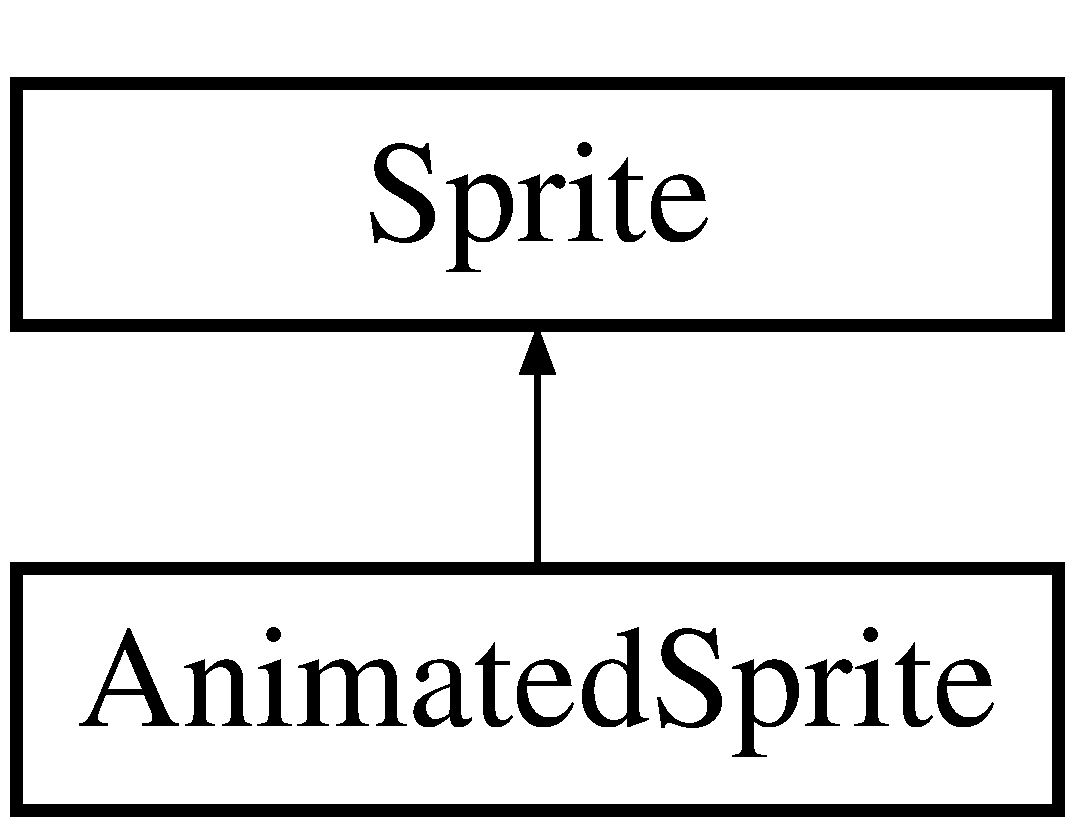
\includegraphics[height=2.000000cm]{class_animated_sprite}
\end{center}
\end{figure}
\subsection*{Public Member Functions}
\begin{DoxyCompactItemize}
\item 
{\bfseries Animated\+Sprite} ({\bf Graphic} \&graphics, const std\+::string \&filepath, int src\+\_\+x, int src\+\_\+y, int width, int height, int fps, int num\+Frames)\label{class_animated_sprite_a2a1f34b3a8a73610e7ab0a8d741af37c}

\item 
void {\bfseries update} (int elapsed\+Time\+Ms)\label{class_animated_sprite_a18757c4843c4022bd1a021e5679ba072}

\end{DoxyCompactItemize}
\subsection*{Private Attributes}
\begin{DoxyCompactItemize}
\item 
const int {\bfseries frame\+Time}\label{class_animated_sprite_a5d2761b7b834c5b0e8f8e96702c4f45b}

\item 
const int {\bfseries num\+Frames}\label{class_animated_sprite_ac89d280976ff63f8cdaf50c6c4dcf640}

\item 
int {\bfseries cur\+Frame}\label{class_animated_sprite_a02d0ef997b93c7376ebdeffd0e6cd061}

\item 
int {\bfseries elapsed\+Time}\label{class_animated_sprite_a3c653a3497872da461b83dfcc3dac040}

\end{DoxyCompactItemize}
\subsection*{Additional Inherited Members}


The documentation for this class was generated from the following files\+:\begin{DoxyCompactItemize}
\item 
C\+:/\+Users/\+Max/\+Documents/\+Git\+Hub/\+Ballerburg/\+Ballerburg\+\_\+v001/animatedsprite.\+h\item 
C\+:/\+Users/\+Max/\+Documents/\+Git\+Hub/\+Ballerburg/\+Ballerburg\+\_\+v001/animatedsprite.\+cpp\end{DoxyCompactItemize}

\section{Backdrop Class Reference}
\label{class_backdrop}\index{Backdrop@{Backdrop}}
\subsection*{Public Member Functions}
\begin{DoxyCompactItemize}
\item 
{\bfseries Backdrop} ({\bf Graphic} \&graphics)\label{class_backdrop_aff823aed9971b23163805ec4e95fc416}

\item 
void {\bfseries draw} ({\bf Graphic} \&graphics)\label{class_backdrop_a29da942a98d4e2abef1eb319d3e91eb5}

\item 
void {\bfseries update} (int elapsed\+Time)\label{class_backdrop_a884306a0b99b02aedcc8ece6d816c316}

\end{DoxyCompactItemize}
\subsection*{Private Attributes}
\begin{DoxyCompactItemize}
\item 
bool {\bfseries direction}\label{class_backdrop_a5fe4ad01deab5b452b58e012f5fb4cb8}

\item 
float {\bfseries pos\+Cloud\+X}\label{class_backdrop_ad5246c7295feb7eb1b702f68fd61cafc}

\item 
float {\bfseries pos\+Cloud\+Y}\label{class_backdrop_a1f64b463a9aee12954ea71fe5a19d24d}

\item 
std\+::unique\+\_\+ptr$<$ {\bf Sprite} $>$ {\bfseries background}\label{class_backdrop_ac5824d5ad0e1787f278b87439d3af8e8}

\item 
std\+::unique\+\_\+ptr$<$ {\bf Sprite} $>$ {\bfseries background\+Cloud}\label{class_backdrop_a07cfdc5c89945db324bfa91277f913bb}

\end{DoxyCompactItemize}


The documentation for this class was generated from the following files\+:\begin{DoxyCompactItemize}
\item 
C\+:/\+Users/\+Max/\+Documents/\+Git\+Hub/\+Ballerburg/\+Ballerburg\+\_\+v001/backdrop.\+h\item 
C\+:/\+Users/\+Max/\+Documents/\+Git\+Hub/\+Ballerburg/\+Ballerburg\+\_\+v001/backdrop.\+cpp\end{DoxyCompactItemize}

\section{Block Class Reference}
\label{class_block}\index{Block@{Block}}
Inheritance diagram for Block\+:\begin{figure}[H]
\begin{center}
\leavevmode
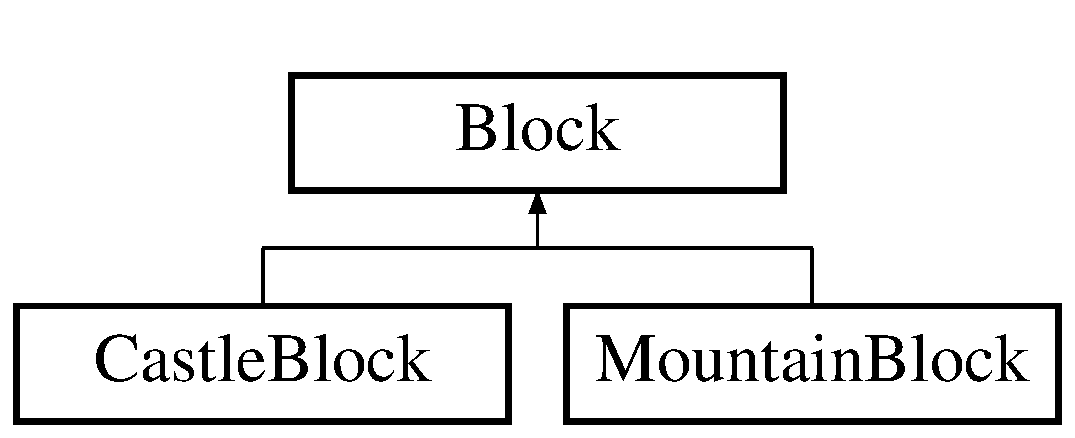
\includegraphics[height=2.000000cm]{class_block}
\end{center}
\end{figure}
\subsection*{Public Member Functions}
\begin{DoxyCompactItemize}
\item 
{\bfseries Block} (int pos\+X, int pos\+Y)\label{class_block_a32b95f86d54a19a55bd7c51a578c28e6}

\item 
void {\bfseries update} ()\label{class_block_a10e17f44df4d273c16190732197578f2}

\item 
void {\bfseries draw} ({\bf Graphic} \&graphics)\label{class_block_a23ca57ffc9fb97f8da3e8620a6718a55}

\item 
void {\bfseries destroy} ()\label{class_block_a27b3bed5a1064d818cd61915f3a380bb}

\item 
void {\bfseries on\+Hit} ({\bf Input} \&in, {\bf Sound} \&sound)\label{class_block_a7263eccd8f8aa3608fa693542add773d}

\item 
bool {\bfseries is\+Hit} ({\bf Input} \&in)\label{class_block_ac4b4ccebb66855f4b8bd234d3bf6d166}

\item 
{\bf S\+D\+L\+\_\+\+Rect} \& {\bfseries get\+Collision\+Rectangle} ()\label{class_block_a719df3c056ce1dc1d93b67275a5c13c1}

\end{DoxyCompactItemize}
\subsection*{Public Attributes}
\begin{DoxyCompactItemize}
\item 
int {\bfseries pos\+X}\label{class_block_ad1db677097e72dd66e59a29f0bbce569}

\item 
int {\bfseries pos\+Y}\label{class_block_a675610bc12401b8d5f494ddae9998916}

\item 
bool {\bfseries hit}\label{class_block_a76234c3996d52d7ddc841c48284feecf}

\item 
std\+::unique\+\_\+ptr$<$ {\bf Sprite} $>$ {\bfseries block\+Sprite}\label{class_block_ac9e117395424b43eced9cee542bbe68b}

\item 
std\+::unique\+\_\+ptr$<$ {\bf S\+D\+L\+\_\+\+Rect} $>$ {\bfseries collision\+Rectangle}\label{class_block_a7720f1fde214267bd9003e2480c96be5}

\end{DoxyCompactItemize}


The documentation for this class was generated from the following files\+:\begin{DoxyCompactItemize}
\item 
C\+:/\+Users/\+Max/\+Documents/\+Git\+Hub/\+Ballerburg/\+Ballerburg\+\_\+v001/block.\+h\item 
C\+:/\+Users/\+Max/\+Documents/\+Git\+Hub/\+Ballerburg/\+Ballerburg\+\_\+v001/block.\+cpp\end{DoxyCompactItemize}

\section{Cannon Class Reference}
\label{class_cannon}\index{Cannon@{Cannon}}
\subsection*{Public Member Functions}
\begin{DoxyCompactItemize}
\item 
{\bfseries Cannon} ({\bf Graphic} \&graphics, int pos\+X, int pos\+Y)\label{class_cannon_a7dc46cea020d9360ce939f5eed18604f}

\item 
void {\bfseries draw} ({\bf Graphic} \&graphics)\label{class_cannon_adc9351fb66c450f50e1ebb71a17ab101}

\item 
void {\bfseries update} (int elapsed\+Time, {\bf Map} \&map)\label{class_cannon_ace63d1bb033c544019f570fcc6d34751}

\item 
void {\bfseries move\+Left} ()\label{class_cannon_a52cda8f88ae6a3bd6220dcaf7f35e275}

\item 
void {\bfseries move\+Right} ()\label{class_cannon_af6c1e5ba6193fd4e4e9c74c8306fa01d}

\item 
void {\bfseries move\+Up} ()\label{class_cannon_a794ccd790953d7a565489a679427a98a}

\item 
void {\bfseries move\+Down} ()\label{class_cannon_aaaab504200dc7755b4a1088646f8c8d6}

\item 
void {\bfseries shoot} ({\bf Graphic} \&graphics)\label{class_cannon_acd07d0e39e049745e8d146a7be1ccf33}

\end{DoxyCompactItemize}
\subsection*{Private Attributes}
\begin{DoxyCompactItemize}
\item 
float {\bfseries pos\+X}\label{class_cannon_a5915116075945ec3928ebf3745f517c7}

\item 
float {\bfseries pos\+Y}\label{class_cannon_a6790466c3b6b779e0d2e0909728decf6}

\item 
std\+::unique\+\_\+ptr$<$ {\bf Cannonball} $>$ {\bfseries ball}\label{class_cannon_a621a4bcec5b09bcc5cfd783439a85e0c}

\item 
std\+::unique\+\_\+ptr$<$ {\bf Sprite} $>$ {\bfseries cannon}\label{class_cannon_a62290a4217593ea492caab58878c4c2d}

\end{DoxyCompactItemize}


The documentation for this class was generated from the following files\+:\begin{DoxyCompactItemize}
\item 
C\+:/\+Users/\+Max/\+Documents/\+Git\+Hub/\+Ballerburg/\+Ballerburg\+\_\+v001/cannon.\+h\item 
C\+:/\+Users/\+Max/\+Documents/\+Git\+Hub/\+Ballerburg/\+Ballerburg\+\_\+v001/cannon.\+cpp\end{DoxyCompactItemize}

\section{Cannonball Class Reference}
\label{class_cannonball}\index{Cannonball@{Cannonball}}
\subsection*{Public Member Functions}
\begin{DoxyCompactItemize}
\item 
{\bfseries Cannonball} ({\bf Graphic} \&graphic, int pos\+X, int pos\+Y)\label{class_cannonball_ae7e8fe5eb3272229d78c221ac4b56a55}

\item 
void {\bfseries update} (int elapsed\+Time, {\bf Map} \&map)\label{class_cannonball_a8bd123a497feecb18da788ec6d724158}

\item 
void {\bfseries update} (int elapsed\+Time, std\+::vector$<$ {\bf Block} $>$ \&map)\label{class_cannonball_a4e9110f4da8a085d2654aa1ed4f2dcb6}

\item 
void {\bfseries draw} ({\bf Graphic} \&graphics)\label{class_cannonball_aa8cb4cb637acbf6b6132f34b0588fd46}

\item 
void {\bfseries move\+Right} ()\label{class_cannonball_ade6097b63fc6d66c14014843a5e84c2e}

\item 
void {\bfseries move\+Left} ()\label{class_cannonball_a00f73b76d893d76a48cf74d3d123c874}

\item 
void {\bfseries move\+Up} ()\label{class_cannonball_af8bcca2d4dd7a84d52bd2d89203ce9cd}

\item 
void {\bfseries move\+Down} ()\label{class_cannonball_af69eb8fff953a77721d63063d82b2650}

\item 
bool {\bfseries has\+Collided} ()\label{class_cannonball_a3c2e8ae577405cd797f7e5bfbeab2e59}

\end{DoxyCompactItemize}
\subsection*{Private Member Functions}
\begin{DoxyCompactItemize}
\item 
double {\bfseries distance} (int x1, int y1, int x2, int y2)\label{class_cannonball_a9e297db446a0a85cf11459b657d26125}

\item 
bool {\bfseries check\+Collision} ({\bf Circle} \&A, {\bf Map} \&B)\label{class_cannonball_a782b1293862fe31273c7de1941e8544a}

\item 
void {\bfseries update\+X} (int elapsed\+Time, {\bf Map} \&map)\label{class_cannonball_aeb159591227b193a1d78f663fc807653}

\item 
void {\bfseries update\+Y} (int elapsed\+Time, {\bf Map} \&map)\label{class_cannonball_a72f41a02fe2101abd082dbb6567715ef}

\end{DoxyCompactItemize}
\subsection*{Private Attributes}
\begin{DoxyCompactItemize}
\item 
int {\bfseries pos\+X}\label{class_cannonball_a36aac6eec38415bb074c09e66cf24f1f}

\item 
int {\bfseries pos\+Y}\label{class_cannonball_a27def66b928e564d5bac7382c66ae5a5}

\item 
bool {\bfseries collided}\label{class_cannonball_a0794a8ae61dc67fab82fcbc24d580100}

\item 
float {\bfseries velocity\+X}\label{class_cannonball_ac384c351b9621cd16ebbd980ba37404d}

\item 
float {\bfseries velocity\+Y}\label{class_cannonball_a0275fa75787a8ddc9e4decead6201a27}

\item 
{\bf Circle} {\bfseries collision\+Circle}\label{class_cannonball_abae8e9805e8931bcbe6d5c83d9dd0a27}

\item 
std\+::unique\+\_\+ptr$<$ {\bf Sprite} $>$ {\bfseries sprite\+Dot}\label{class_cannonball_a90ddfd584ef92517b2ca3d1de600a7e6}

\end{DoxyCompactItemize}


The documentation for this class was generated from the following files\+:\begin{DoxyCompactItemize}
\item 
C\+:/\+Users/\+Max/\+Documents/\+Git\+Hub/\+Ballerburg/\+Ballerburg\+\_\+v001/cannonball.\+h\item 
C\+:/\+Users/\+Max/\+Documents/\+Git\+Hub/\+Ballerburg/\+Ballerburg\+\_\+v001/cannonball.\+cpp\end{DoxyCompactItemize}

\section{Castle Class Reference}
\label{class_castle}\index{Castle@{Castle}}
\subsection*{Public Member Functions}
\begin{DoxyCompactItemize}
\item 
{\bfseries Castle} ({\bf Graphic} \&graphics, int startpos\+X)\label{class_castle_ab5ec93846d60e52722de92e45c753d4b}

\item 
void {\bfseries update} ({\bf Input} \&input, {\bf Sound} \&sound)\label{class_castle_a88b3dd90f1c6a9bc4f84deb5bed8ea97}

\item 
void {\bfseries draw} ({\bf Graphic} \&graphics)\label{class_castle_a0b25b9dead62c64e7e48a587453b1138}

\item 
void {\bfseries check\+Hit} ({\bf Input} \&in, {\bf Sound} \&sound)\label{class_castle_a8c40e91a3d1ae3dba9003607736c8076}

\item 
std\+::vector$<$ {\bf S\+D\+L\+\_\+\+Rect} $>$ {\bfseries get\+Map} ()\label{class_castle_a94e009f51990bf1fe4e65c6809848480}

\item 
void {\bfseries delete\+Block} (int index)\label{class_castle_a33d197526444e9899ff601342671efe2}

\item 
{\bf Castle\+Block} \& {\bfseries get\+Block} (int block)\label{class_castle_a540a311c65db41018f12a9da996f01b4}

\end{DoxyCompactItemize}


The documentation for this class was generated from the following files\+:\begin{DoxyCompactItemize}
\item 
C\+:/\+Users/\+Max/\+Documents/\+Git\+Hub/\+Ballerburg/\+Ballerburg\+\_\+v001/castle.\+h\item 
C\+:/\+Users/\+Max/\+Documents/\+Git\+Hub/\+Ballerburg/\+Ballerburg\+\_\+v001/castle.\+cpp\end{DoxyCompactItemize}

\section{Castle\+Block Class Reference}
\label{class_castle_block}\index{Castle\+Block@{Castle\+Block}}
Inheritance diagram for Castle\+Block\+:\begin{figure}[H]
\begin{center}
\leavevmode
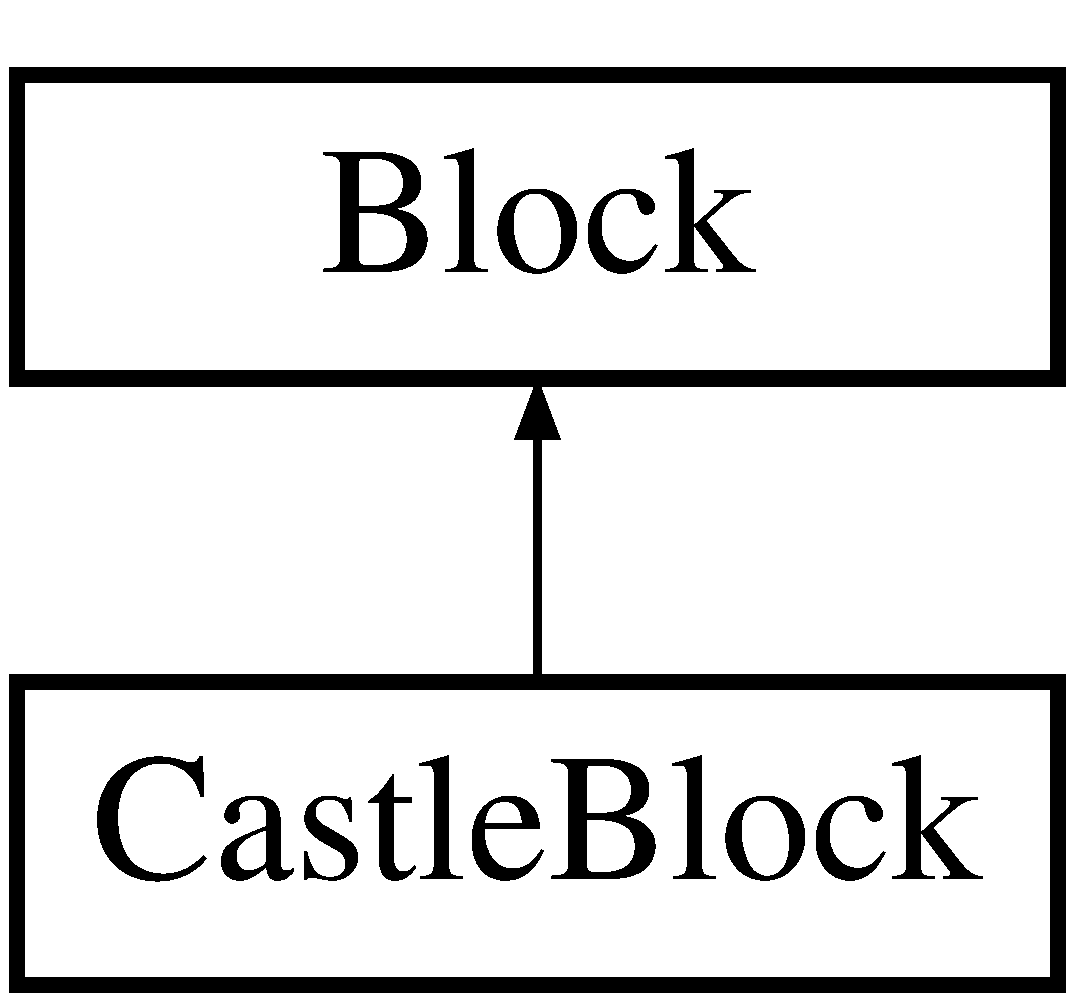
\includegraphics[height=2.000000cm]{class_castle_block}
\end{center}
\end{figure}
\subsection*{Public Member Functions}
\begin{DoxyCompactItemize}
\item 
{\bfseries Castle\+Block} ({\bf Graphic} \&graphics, int type\+Number, int pos\+X, int pos\+Y)\label{class_castle_block_a671cb6316ce4692c603c3c5fac39dbf5}

\item 
void {\bfseries destroy} ()\label{class_castle_block_af3bdbe064632c9b75a1139a97ae04748}

\end{DoxyCompactItemize}
\subsection*{Additional Inherited Members}


The documentation for this class was generated from the following files\+:\begin{DoxyCompactItemize}
\item 
C\+:/\+Users/\+Max/\+Documents/\+Git\+Hub/\+Ballerburg/\+Ballerburg\+\_\+v001/castleblock.\+h\item 
C\+:/\+Users/\+Max/\+Documents/\+Git\+Hub/\+Ballerburg/\+Ballerburg\+\_\+v001/castleblock.\+cpp\end{DoxyCompactItemize}

\section{Castleblock\+O\+L\+D Class Reference}
\label{class_castleblock_o_l_d}\index{Castleblock\+O\+L\+D@{Castleblock\+O\+L\+D}}
\subsection*{Public Member Functions}
\begin{DoxyCompactItemize}
\item 
{\bfseries Castleblock\+O\+L\+D} ({\bf Graphic} \&graphics, int pos\+X, int pos\+Y, const std\+::string \&file\+Path)\label{class_castleblock_o_l_d_a8ad1f97522837dec4a32a13191f903a4}

\item 
void {\bfseries on\+Hit} ({\bf Input} \&in, {\bf Sound} \&sound)\label{class_castleblock_o_l_d_a544647c3b75536335078646b18e47ccb}

\item 
void {\bfseries draw} ({\bf Graphic} \&draw)\label{class_castleblock_o_l_d_a21f1c02d6abdd9608fab3be81d4c7361}

\end{DoxyCompactItemize}
\subsection*{Private Member Functions}
\begin{DoxyCompactItemize}
\item 
bool {\bfseries is\+Hit} ({\bf Input} \&in)\label{class_castleblock_o_l_d_a083e06e6e9f7ad729f9ffb3f750b6842}

\end{DoxyCompactItemize}
\subsection*{Private Attributes}
\begin{DoxyCompactItemize}
\item 
bool {\bfseries hit}\label{class_castleblock_o_l_d_ae4140cd84e64c1cba92109812b08f7bf}

\item 
int {\bfseries x}\label{class_castleblock_o_l_d_a41c5d96c49f29514580a64e5cd17e0b8}

\item 
int {\bfseries y}\label{class_castleblock_o_l_d_a6dbf64ae7dde90f8ea1edda3c382da0f}

\item 
std\+::unique\+\_\+ptr$<$ {\bf Sprite} $>$ {\bfseries cblock}\label{class_castleblock_o_l_d_afe01828923fa2d64c60cd4b957b0a865}

\end{DoxyCompactItemize}


The documentation for this class was generated from the following files\+:\begin{DoxyCompactItemize}
\item 
C\+:/\+Users/\+Max/\+Documents/\+Git\+Hub/\+Ballerburg/\+Ballerburg\+\_\+v001/castleblockold.\+h\item 
C\+:/\+Users/\+Max/\+Documents/\+Git\+Hub/\+Ballerburg/\+Ballerburg\+\_\+v001/castleblockold.\+cpp\end{DoxyCompactItemize}

\section{Circle Class Reference}
\label{class_circle}\index{Circle@{Circle}}


Dies ist eine kleine Klasse, die einen einfachen Kreis realisiert.  




{\ttfamily \#include $<$circle.\+h$>$}

\subsection*{Public Member Functions}
\begin{DoxyCompactItemize}
\item 
{\bfseries Circle} (int offset\+X, int offset\+Y, int radius)\label{class_circle_a899b70433bcb874e6eab17a5d56fc6aa}

\end{DoxyCompactItemize}
\subsection*{Public Attributes}
\begin{DoxyCompactItemize}
\item 
int {\bfseries x}\label{class_circle_abceecd15b990054ddc30441cfcbb205d}

\item 
int {\bf y}
\item 
int {\bf r}
\end{DoxyCompactItemize}


\subsection{Detailed Description}
Dies ist eine kleine Klasse, die einen einfachen Kreis realisiert. 

\subsection{Member Data Documentation}
\index{Circle@{Circle}!r@{r}}
\index{r@{r}!Circle@{Circle}}
\subsubsection[{r}]{\setlength{\rightskip}{0pt plus 5cm}int Circle\+::r}\label{class_circle_a067c0b8ccbda5ca1f518dd89a1d55989}
Radius des Kreises \index{Circle@{Circle}!y@{y}}
\index{y@{y}!Circle@{Circle}}
\subsubsection[{y}]{\setlength{\rightskip}{0pt plus 5cm}int Circle\+::y}\label{class_circle_a78aef28b3c176d14e8d25f8cd84e7dfd}
Offset von der Mitte des Kreises 

The documentation for this class was generated from the following file\+:\begin{DoxyCompactItemize}
\item 
C\+:/\+Users/\+Max/\+Documents/\+Git\+Hub/\+Ballerburg/\+Ballerburg\+\_\+v001/circle.\+h\end{DoxyCompactItemize}

\section{Game Class Reference}
\label{class_game}\index{Game@{Game}}
\subsection*{Static Public Member Functions}
\begin{DoxyCompactItemize}
\item 
static void {\bfseries end\+Game} ()\label{class_game_a1dd53b1421401d56b123448b3009ec42}

\end{DoxyCompactItemize}
\subsection*{Static Public Attributes}
\begin{DoxyCompactItemize}
\item 
static int {\bfseries k\+Screen\+Width} = 640\label{class_game_a5cd5507c48083efe21870edc010b0092}

\item 
static int {\bfseries k\+Screen\+Height} = 360\label{class_game_a987ce043b9c2dca54691ddc4146b6411}

\item 
static bool {\bfseries running} = true\label{class_game_a8ca5b9f8a62990e6022de17785beac2c}

\end{DoxyCompactItemize}
\subsection*{Private Member Functions}
\begin{DoxyCompactItemize}
\item 
void {\bfseries game\+Loop} ()\label{class_game_aede5f46c8c7bbbaf8459eeec397a11e7}

\item 
void {\bfseries update} (int elapsed\+Time, {\bf Map} \&map, {\bf Input} \&input, {\bf Sound} \&sound)\label{class_game_a500c9c05c044487957dfc3c7e5d7df99}

\item 
void {\bfseries draw} ({\bf Graphic} \&graphics)\label{class_game_adddab9024dc030c923651ed737f1f6b5}

\end{DoxyCompactItemize}
\subsection*{Private Attributes}
\begin{DoxyCompactItemize}
\item 
std\+::unique\+\_\+ptr$<$ {\bf Backdrop} $>$ {\bfseries background}\label{class_game_a023bc00208cfb619bc770ae70960e324}

\item 
std\+::unique\+\_\+ptr$<$ {\bf Cannon} $>$ {\bfseries cannon}\label{class_game_aac35f37418de999e504f85448b57cb57}

\item 
std\+::unique\+\_\+ptr$<$ {\bf Sound} $>$ {\bfseries sounds}\label{class_game_aca7489006293a79030b68c0e8e4d0029}

\item 
std\+::unique\+\_\+ptr$<$ {\bf Map} $>$ {\bfseries map}\label{class_game_adc3f6b00e354d21502a62e375360911f}

\end{DoxyCompactItemize}


The documentation for this class was generated from the following files\+:\begin{DoxyCompactItemize}
\item 
C\+:/\+Users/\+Max/\+Documents/\+Git\+Hub/\+Ballerburg/\+Ballerburg\+\_\+v001/game.\+h\item 
C\+:/\+Users/\+Max/\+Documents/\+Git\+Hub/\+Ballerburg/\+Ballerburg\+\_\+v001/game.\+cpp\end{DoxyCompactItemize}

\section{Graphic Class Reference}
\label{class_graphic}\index{Graphic@{Graphic}}


Die Klasse \doxyref{Graphic}{p.}{class_graphic} dient als zentrales Objekt, wenn es um das Laden und Darstellen von Sprites geht.  




{\ttfamily \#include $<$graphic.\+h$>$}

\subsection*{Public Types}
\begin{DoxyCompactItemize}
\item 
typedef {\bf S\+D\+L\+\_\+\+Surface} $\ast$ {\bfseries Surface\+I\+D}\label{class_graphic_a089a4ef41832ffbc00306774c279c262}

\end{DoxyCompactItemize}
\subsection*{Public Member Functions}
\begin{DoxyCompactItemize}
\item 
{\bf Surface\+I\+D} {\bf load\+Image} (const std\+::string \&file\+Path)
\begin{DoxyCompactList}\small\item\em Lädt eine Datei und setzt einen Color\+Key (entfernt R\+G\+B\+: 255, 0, 255) \end{DoxyCompactList}\item 
void {\bf blit\+Surface} ({\bf Surface\+I\+D} src, {\bf S\+D\+L\+\_\+\+Rect} $\ast$src\+\_\+rectangle, {\bf S\+D\+L\+\_\+\+Rect} $\ast$dest\+\_\+rectangle)
\begin{DoxyCompactList}\small\item\em zeichnet ein Surface auf den Screen \end{DoxyCompactList}\item 
void {\bf clean\+Up} ()\label{class_graphic_a15c85c04c5b78994c94013827e6095ea}

\begin{DoxyCompactList}\small\item\em Säubert den Screen nach jedem Frame, indem er alles löscht. Dies verhindert Artefakte aus dem letzten Frame im neuen Frame. \end{DoxyCompactList}\item 
void {\bf flip} ()
\begin{DoxyCompactList}\small\item\em Da der Screen als doppelter Puffer in S\+D\+L realisiert wird muss der Screen \char`\"{}umgedreht\char`\"{} werden. \end{DoxyCompactList}\end{DoxyCompactItemize}
\subsection*{Private Types}
\begin{DoxyCompactItemize}
\item 
typedef std\+::map$<$ std\+::string, {\bf S\+D\+L\+\_\+\+Surface} $\ast$ $>$ {\bf Sprite\+Map}
\end{DoxyCompactItemize}
\subsection*{Private Attributes}
\begin{DoxyCompactItemize}
\item 
{\bf Sprite\+Map} {\bf sprite\+Sheets}
\item 
{\bf S\+D\+L\+\_\+\+Surface} $\ast$ {\bf screen}
\end{DoxyCompactItemize}


\subsection{Detailed Description}
Die Klasse \doxyref{Graphic}{p.}{class_graphic} dient als zentrales Objekt, wenn es um das Laden und Darstellen von Sprites geht. 

Alle Grafiken werden in einer \doxyref{Map}{p.}{class_map} organisiert und mit Hilfe der blit\+Surface Methode auf dem Screen angebracht

\begin{DoxySeeAlso}{See also}
\doxyref{sprite.\+h}{p.}{sprite_8h_source} 

\doxyref{animated\+Sprite.\+h}{p.}{animatedsprite_8h_source}
\end{DoxySeeAlso}
\begin{DoxyAuthor}{Author}
Max Niederauer 
\end{DoxyAuthor}


\subsection{Member Typedef Documentation}
\index{Graphic@{Graphic}!Sprite\+Map@{Sprite\+Map}}
\index{Sprite\+Map@{Sprite\+Map}!Graphic@{Graphic}}
\subsubsection[{Sprite\+Map}]{\setlength{\rightskip}{0pt plus 5cm}typedef std\+::map$<$std\+::string, {\bf S\+D\+L\+\_\+\+Surface}$\ast$$>$ {\bf Graphic\+::\+Sprite\+Map}\hspace{0.3cm}{\ttfamily [private]}}\label{class_graphic_aa06a625a3faeaccd5613e8623d59ae4e}
Definition eines eigenen Types Sprite\+Map 

\subsection{Member Function Documentation}
\index{Graphic@{Graphic}!blit\+Surface@{blit\+Surface}}
\index{blit\+Surface@{blit\+Surface}!Graphic@{Graphic}}
\subsubsection[{blit\+Surface}]{\setlength{\rightskip}{0pt plus 5cm}void Graphic\+::blit\+Surface (
\begin{DoxyParamCaption}
\item[{{\bf Surface\+I\+D}}]{src, }
\item[{{\bf S\+D\+L\+\_\+\+Rect} $\ast$}]{src\+\_\+rectangle, }
\item[{{\bf S\+D\+L\+\_\+\+Rect} $\ast$}]{dest\+\_\+rectangle}
\end{DoxyParamCaption}
)}\label{class_graphic_ae2ab1b6e70958efae02f7131493740ff}


zeichnet ein Surface auf den Screen 


\begin{DoxyParams}{Parameters}
{\em src} & -\/ Surface, welches auf den Screen gezeichnet werden soll \\
\hline
{\em src\+\_\+rectangle} & -\/ definiert wo und wie groß das Surface gezeichnet werden soll (beinhaltet das Surface) \\
\hline
{\em dest\+\_\+rectangle} & -\/ das engültige Ziel des Surfaces \\
\hline
\end{DoxyParams}
\index{Graphic@{Graphic}!flip@{flip}}
\index{flip@{flip}!Graphic@{Graphic}}
\subsubsection[{flip}]{\setlength{\rightskip}{0pt plus 5cm}void Graphic\+::flip (
\begin{DoxyParamCaption}
{}
\end{DoxyParamCaption}
)}\label{class_graphic_af3dd8fed2b2384149643116bdb813c01}


Da der Screen als doppelter Puffer in S\+D\+L realisiert wird muss der Screen \char`\"{}umgedreht\char`\"{} werden. 

\begin{DoxySeeAlso}{See also}
\doxyref{S\+D\+L/\+S\+D\+L.\+h}{p.}{_s_d_l_8h} 
\end{DoxySeeAlso}
\index{Graphic@{Graphic}!load\+Image@{load\+Image}}
\index{load\+Image@{load\+Image}!Graphic@{Graphic}}
\subsubsection[{load\+Image}]{\setlength{\rightskip}{0pt plus 5cm}{\bf Graphic\+::\+Surface\+I\+D} Graphic\+::load\+Image (
\begin{DoxyParamCaption}
\item[{const std\+::string \&}]{file\+Path}
\end{DoxyParamCaption}
)}\label{class_graphic_a259fd9b61b67a164094bf9ba0b5044cd}


Lädt eine Datei und setzt einen Color\+Key (entfernt R\+G\+B\+: 255, 0, 255) 


\begin{DoxyParams}{Parameters}
{\em file\+Path} & -\/ Dateipfad zu der Datei, die geladen werden soll \\
\hline
\end{DoxyParams}
\begin{DoxyReturn}{Returns}
gibt das Surface zurück auf welches die Datei geladen wurde 
\end{DoxyReturn}


\subsection{Member Data Documentation}
\index{Graphic@{Graphic}!screen@{screen}}
\index{screen@{screen}!Graphic@{Graphic}}
\subsubsection[{screen}]{\setlength{\rightskip}{0pt plus 5cm}{\bf S\+D\+L\+\_\+\+Surface}$\ast$ Graphic\+::screen\hspace{0.3cm}{\ttfamily [private]}}\label{class_graphic_a395202e12873a72645439fe6a202d0d2}
Der Screen auf den alle Surfaces gezeichnet werden \index{Graphic@{Graphic}!sprite\+Sheets@{sprite\+Sheets}}
\index{sprite\+Sheets@{sprite\+Sheets}!Graphic@{Graphic}}
\subsubsection[{sprite\+Sheets}]{\setlength{\rightskip}{0pt plus 5cm}{\bf Sprite\+Map} Graphic\+::sprite\+Sheets\hspace{0.3cm}{\ttfamily [private]}}\label{class_graphic_ad552ac2423b445b7c58be50a484d886b}
std\+::map, die die Sprites organisiert 

The documentation for this class was generated from the following files\+:\begin{DoxyCompactItemize}
\item 
C\+:/\+Users/\+Max/\+Documents/\+Git\+Hub/\+Ballerburg/\+Ballerburg\+\_\+v001/graphic.\+h\item 
C\+:/\+Users/\+Max/\+Documents/\+Git\+Hub/\+Ballerburg/\+Ballerburg\+\_\+v001/graphic.\+cpp\end{DoxyCompactItemize}

\section{Input Class Reference}
\label{class_input}\index{Input@{Input}}
\subsection*{Public Member Functions}
\begin{DoxyCompactItemize}
\item 
void {\bfseries begin\+New\+Frame} ()\label{class_input_ac82c7c0bdc0b672b8d1354303ad09235}

\item 
void {\bfseries key\+Up\+Event} (const {\bf S\+D\+L\+\_\+\+Event} \&event)\label{class_input_af7975123c8e7bf107d3ffeb7e8c7ac62}

\item 
void {\bfseries key\+Down\+Event} (const {\bf S\+D\+L\+\_\+\+Event} \&event)\label{class_input_a2bcc16ac90c1001921978e6a2c470242}

\item 
void {\bfseries mouse\+Event} (const {\bf S\+D\+L\+\_\+\+Event} \&event)\label{class_input_a33758e5fc972c30d2effca8c45af2a3d}

\item 
bool {\bfseries was\+Left\+Mouse\+Button\+Pressed} ()\label{class_input_a0dad9a60338030fae228726f7d76bfe1}

\item 
bool {\bfseries was\+Key\+Pressed} (S\+D\+L\+Key key)\label{class_input_a20a05eafeefe8f0a4a901d8c23c862e6}

\item 
bool {\bfseries was\+Key\+Released} (S\+D\+L\+Key key)\label{class_input_a40f4e0bef7deaf1b81c517c8d2e4e08c}

\item 
bool {\bfseries is\+Key\+Held} (S\+D\+L\+Key key)\label{class_input_af69e24c9d691c43f56a4afc20d56a081}

\item 
void {\bfseries check\+Input} ({\bf S\+D\+L\+\_\+\+Event} \&event)\label{class_input_a6ea35796697b6be39118d7d51e8a47a5}

\item 
void {\bfseries move\+Cannonball} ({\bf Cannon} \&ball, {\bf Graphic} \&graphics)\label{class_input_a021cb5427da09e513b4ac4ed60f7b178}

\item 
int {\bfseries getoffset\+X} () const \label{class_input_a3f79c2144849f550f9102856d46d3d59}

\item 
int {\bfseries getoffset\+Y} () const \label{class_input_a76e210586ca26895c80af7268475187f}

\end{DoxyCompactItemize}


The documentation for this class was generated from the following files\+:\begin{DoxyCompactItemize}
\item 
C\+:/\+Users/\+Max/\+Documents/\+Git\+Hub/\+Ballerburg/\+Ballerburg\+\_\+v001/input.\+h\item 
C\+:/\+Users/\+Max/\+Documents/\+Git\+Hub/\+Ballerburg/\+Ballerburg\+\_\+v001/input.\+cpp\end{DoxyCompactItemize}

\section{King Class Reference}
\label{class_king}\index{King@{King}}
\subsection*{Public Member Functions}
\begin{DoxyCompactItemize}
\item 
{\bfseries King} ({\bf Graphic} \&graphics, int pos\+X, int pos\+Y)\label{class_king_ac559c45c410e8e356ac51f55dfec490e}

\item 
void {\bfseries update} ({\bf Input} \&in, {\bf Sound} \&sound)\label{class_king_ae8f4b316eb44ecf9a3f4cef12f20abb4}

\item 
void {\bfseries draw} ({\bf Graphic} \&graphics)\label{class_king_a302fd53f1beb9fd5c7f159ef58675d08}

\item 
void {\bfseries destroy} ()\label{class_king_a29c32eddd07de4c75100c06d969858ab}

\item 
void {\bfseries on\+Hit} ({\bf Input} \&in, {\bf Sound} \&sound)\label{class_king_a2c44b8cbdec8153b88041ee7298dc332}

\item 
void {\bfseries disable} ()\label{class_king_a22278859a9a802b9593bed6509c47808}

\item 
{\bf S\+D\+L\+\_\+\+Rect} \& {\bfseries get\+Collision\+Rectangle} ()\label{class_king_ae356b9770f435e7ddb98cfd3816df51c}

\end{DoxyCompactItemize}


The documentation for this class was generated from the following files\+:\begin{DoxyCompactItemize}
\item 
C\+:/\+Users/\+Max/\+Documents/\+Git\+Hub/\+Ballerburg/\+Ballerburg\+\_\+v001/king.\+h\item 
C\+:/\+Users/\+Max/\+Documents/\+Git\+Hub/\+Ballerburg/\+Ballerburg\+\_\+v001/king.\+cpp\end{DoxyCompactItemize}

\section{Map Class Reference}
\label{class_map}\index{Map@{Map}}
\subsection*{Public Member Functions}
\begin{DoxyCompactItemize}
\item 
void {\bfseries draw} ({\bf Graphic} \&graphics)\label{class_map_a07da7aa49b7e6c2303457f06b77dfe6d}

\item 
void {\bfseries update} ({\bf Input} \&input, {\bf Sound} \&sound)\label{class_map_a9b4f56b49f490960afba683133d1e5a3}

\item 
void {\bfseries delete\+Block} (int index)\label{class_map_a2d27fba103ade6c2e812e14fccc80c7e}

\item 
std\+::vector$<$ {\bf S\+D\+L\+\_\+\+Rect} $>$ \& {\bfseries get\+Collision\+Map} ()\label{class_map_af4b9b63a7cfec5e0a868792d69a3d2e7}

\end{DoxyCompactItemize}
\subsection*{Static Public Member Functions}
\begin{DoxyCompactItemize}
\item 
static {\bf Map} $\ast$ {\bfseries create\+Map} ({\bf Graphic} \&graphics)\label{class_map_a36b46cde48bb7113ab054d3125fbca3f}

\end{DoxyCompactItemize}
\subsection*{Public Attributes}
\begin{DoxyCompactItemize}
\item 
std\+::vector$<$ {\bf S\+D\+L\+\_\+\+Rect} $>$ {\bfseries map\+Collision}\label{class_map_a6a18a7d33100d4518791d1c5b0841b98}

\item 
std\+::vector$<$ {\bf Block} $>$ {\bfseries map\+Blocks}\label{class_map_a53c68143f9c94eaea2832174925db2ac}

\item 
std\+::unique\+\_\+ptr$<$ {\bf Castle} $>$ {\bfseries testcastle}\label{class_map_a3c781a3358eb0ccde6c8b407786f81f3}

\item 
std\+::unique\+\_\+ptr$<$ {\bf Castle} $>$ {\bfseries testcastle2}\label{class_map_afb6ecf3a1491a5979cb3d8c2ddfc6289}

\item 
std\+::unique\+\_\+ptr$<$ {\bf Mountain} $>$ {\bfseries mountain}\label{class_map_a10538172aeace3ebbbcff50bfb9d5132}

\item 
std\+::unique\+\_\+ptr$<$ {\bf King} $>$ {\bfseries king1}\label{class_map_a42cfc420f9e8066d6cb894d1c5efb225}

\item 
std\+::unique\+\_\+ptr$<$ {\bf King} $>$ {\bfseries king2}\label{class_map_ab0c064cac3fb14f96e7ae7b75c961e7d}

\end{DoxyCompactItemize}


The documentation for this class was generated from the following files\+:\begin{DoxyCompactItemize}
\item 
C\+:/\+Users/\+Max/\+Documents/\+Git\+Hub/\+Ballerburg/\+Ballerburg\+\_\+v001/map.\+h\item 
C\+:/\+Users/\+Max/\+Documents/\+Git\+Hub/\+Ballerburg/\+Ballerburg\+\_\+v001/map.\+cpp\end{DoxyCompactItemize}

\section{Mix\+\_\+\+Chunk Struct Reference}
\label{struct_mix___chunk}\index{Mix\+\_\+\+Chunk@{Mix\+\_\+\+Chunk}}
\subsection*{Public Attributes}
\begin{DoxyCompactItemize}
\item 
int {\bfseries allocated}\label{struct_mix___chunk_a7b985b90b5f97fffe34834116a281615}

\item 
Uint8 $\ast$ {\bfseries abuf}\label{struct_mix___chunk_a30b3b1a72677d076a1caa72422bb3774}

\item 
Uint32 {\bfseries alen}\label{struct_mix___chunk_a958507964471fc4b9fa0d215f1852d05}

\item 
Uint8 {\bfseries volume}\label{struct_mix___chunk_afc566fd5da7f0ed1f3577f5bc0eac319}

\end{DoxyCompactItemize}


The documentation for this struct was generated from the following file\+:\begin{DoxyCompactItemize}
\item 
C\+:/\+Users/\+Max/\+Documents/\+Git\+Hub/\+Ballerburg/\+Ballerburg\+\_\+v001/\+Resources/\+S\+D\+L-\/1.\+2.\+15/include/\+S\+D\+L/S\+D\+L\+\_\+mixer.\+h\end{DoxyCompactItemize}

\section{Mountain Class Reference}
\label{class_mountain}\index{Mountain@{Mountain}}
\subsection*{Public Member Functions}
\begin{DoxyCompactItemize}
\item 
{\bfseries Mountain} ({\bf Graphic} \&graphics)\label{class_mountain_ae5e5250815fe5cf2f8448a331c8c7604}

\item 
void {\bfseries update} ({\bf Input} \&input, {\bf Sound} \&sound)\label{class_mountain_ab0ebe70029e2bf21d50d7f0517217e12}

\item 
void {\bfseries draw} ({\bf Graphic} \&graphics)\label{class_mountain_acc7a7808b86e6e6ccd50684fb10a884c}

\item 
void {\bfseries check\+Hit} ({\bf Input} \&in, {\bf Sound} \&sound)\label{class_mountain_a5cf0e34242918fdf2f197c8a08bc6721}

\item 
std\+::vector$<$ {\bf S\+D\+L\+\_\+\+Rect} $>$ {\bfseries get\+Map} ()\label{class_mountain_a052e5b287efe7e11c90ce0af651b349f}

\item 
void {\bfseries delete\+Block} (int index)\label{class_mountain_ab15bc8f4bb480c9553e05d2755eb2e90}

\end{DoxyCompactItemize}


The documentation for this class was generated from the following files\+:\begin{DoxyCompactItemize}
\item 
C\+:/\+Users/\+Max/\+Documents/\+Git\+Hub/\+Ballerburg/\+Ballerburg\+\_\+v001/mountain.\+h\item 
C\+:/\+Users/\+Max/\+Documents/\+Git\+Hub/\+Ballerburg/\+Ballerburg\+\_\+v001/mountain.\+cpp\end{DoxyCompactItemize}

\section{Mountain\+Block Class Reference}
\label{class_mountain_block}\index{Mountain\+Block@{Mountain\+Block}}
Inheritance diagram for Mountain\+Block\+:\begin{figure}[H]
\begin{center}
\leavevmode
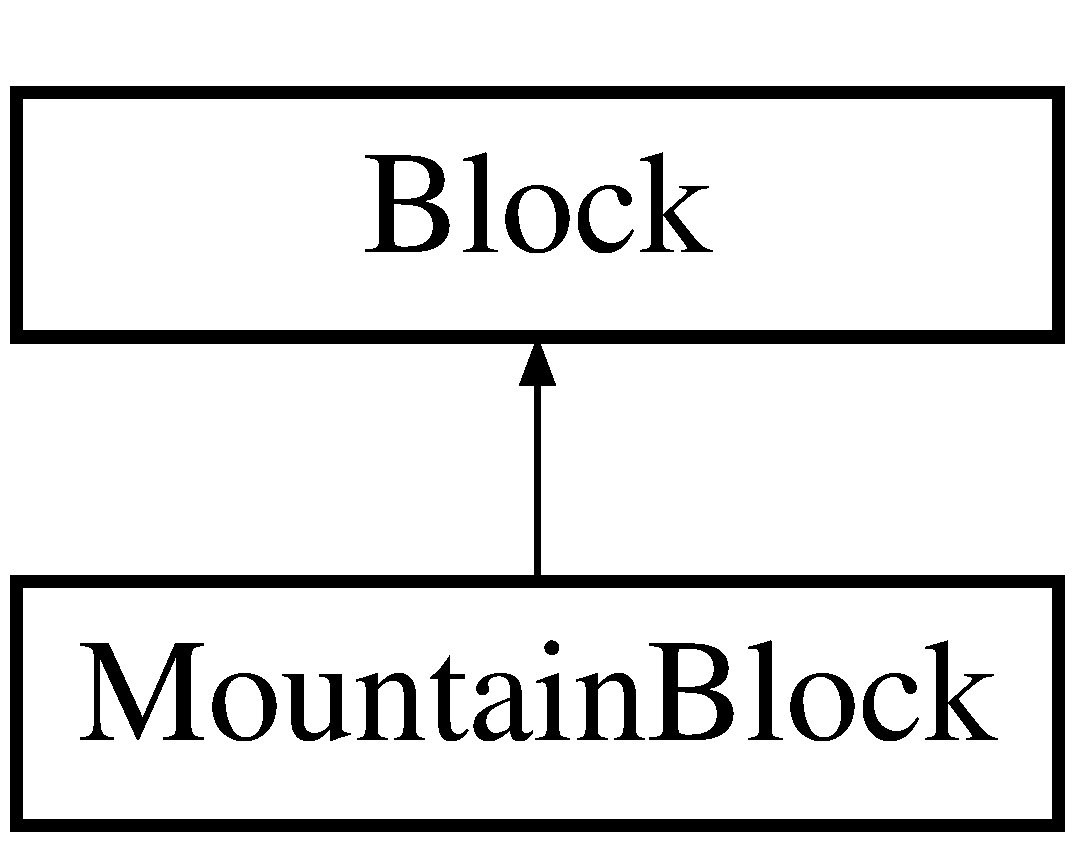
\includegraphics[height=2.000000cm]{class_mountain_block}
\end{center}
\end{figure}
\subsection*{Public Member Functions}
\begin{DoxyCompactItemize}
\item 
{\bfseries Mountain\+Block} ({\bf Graphic} \&graphics, int pos\+X, int pos\+Y)\label{class_mountain_block_a0a4ab12f0943bf6b767f1ead39b6a895}

\item 
void {\bfseries destroy} ()\label{class_mountain_block_ae556e11d2339dc3b586f70b739d0281d}

\end{DoxyCompactItemize}
\subsection*{Additional Inherited Members}


The documentation for this class was generated from the following files\+:\begin{DoxyCompactItemize}
\item 
C\+:/\+Users/\+Max/\+Documents/\+Git\+Hub/\+Ballerburg/\+Ballerburg\+\_\+v001/mountainblock.\+h\item 
C\+:/\+Users/\+Max/\+Documents/\+Git\+Hub/\+Ballerburg/\+Ballerburg\+\_\+v001/mountainblock.\+cpp\end{DoxyCompactItemize}

\section{Rectangle Class Reference}
\label{class_rectangle}\index{Rectangle@{Rectangle}}
\subsection*{Public Member Functions}
\begin{DoxyCompactItemize}
\item 
{\bfseries Rectangle} (int x, int y, int width, int height)\label{class_rectangle_a6fd48c1264965fd841b2d35b7736a352}

\item 
int {\bfseries left} () const \label{class_rectangle_a1f169cef3c9b8307e8dc7c6093bfdd14}

\item 
int {\bfseries right} () const \label{class_rectangle_a8e76ee84d39c8c063cb2ef0e1cb7f5df}

\item 
int {\bfseries top} () const \label{class_rectangle_a8eb6de2c6d532b2175bddd8484196eab}

\item 
int {\bfseries bottom} () const \label{class_rectangle_a46e18ff7c2ca4fd068442cabcd0b4046}

\item 
int {\bfseries get\+Width} () const \label{class_rectangle_a691ea1a449cad163e27bbf10ce65f98d}

\item 
int {\bfseries get\+Height} () const \label{class_rectangle_a45c28d3fd6b2f303530fb80b90e1c1c4}

\item 
void {\bfseries reassign} (int x, int y, int width, int height)\label{class_rectangle_a7f08779a8dbbd7cbf9ca6d8d31e272f8}

\item 
bool {\bfseries collides\+With} (const {\bf Rectangle} \&other) const \label{class_rectangle_a42278a22dbcfdfc05b22eebf7a9bda5d}

\end{DoxyCompactItemize}


The documentation for this class was generated from the following file\+:\begin{DoxyCompactItemize}
\item 
C\+:/\+Users/\+Max/\+Documents/\+Git\+Hub/\+Ballerburg/\+Ballerburg\+\_\+v001/rectangle.\+h\end{DoxyCompactItemize}

\section{S\+D\+L\+\_\+\+Active\+Event Struct Reference}
\label{struct_s_d_l___active_event}\index{S\+D\+L\+\_\+\+Active\+Event@{S\+D\+L\+\_\+\+Active\+Event}}


Application visibility event structure.  




{\ttfamily \#include $<$S\+D\+L\+\_\+events.\+h$>$}

\subsection*{Public Attributes}
\begin{DoxyCompactItemize}
\item 
Uint8 {\bf type}\label{struct_s_d_l___active_event_a4a719c0224f4c0079043432f540621c4}

\begin{DoxyCompactList}\small\item\em S\+D\+L\+\_\+\+A\+C\+T\+I\+V\+E\+E\+V\+E\+N\+T. \end{DoxyCompactList}\item 
Uint8 {\bf gain}\label{struct_s_d_l___active_event_a4887e4fa212696de9fa8803691dfe5c9}

\begin{DoxyCompactList}\small\item\em Whether given states were gained or lost (1/0) \end{DoxyCompactList}\item 
Uint8 {\bf state}\label{struct_s_d_l___active_event_af8f060502a9c906b25a4aa9c61f745f9}

\begin{DoxyCompactList}\small\item\em A mask of the focus states. \end{DoxyCompactList}\end{DoxyCompactItemize}


\subsection{Detailed Description}
Application visibility event structure. 

The documentation for this struct was generated from the following file\+:\begin{DoxyCompactItemize}
\item 
C\+:/\+Users/\+Max/\+Documents/\+Git\+Hub/\+Ballerburg/\+Ballerburg\+\_\+v001/\+Resources/\+S\+D\+L-\/1.\+2.\+15/include/\+S\+D\+L/{\bf S\+D\+L\+\_\+events.\+h}\end{DoxyCompactItemize}

\section{S\+D\+L\+\_\+\+Audio\+C\+V\+T Struct Reference}
\label{struct_s_d_l___audio_c_v_t}\index{S\+D\+L\+\_\+\+Audio\+C\+V\+T@{S\+D\+L\+\_\+\+Audio\+C\+V\+T}}


{\ttfamily \#include $<$S\+D\+L\+\_\+audio.\+h$>$}

\subsection*{Public Member Functions}
\begin{DoxyCompactItemize}
\item 
{\bfseries void} ({\bf S\+D\+L\+C\+A\+L\+L} $\ast$filters[10])(struct {\bf S\+D\+L\+\_\+\+Audio\+C\+V\+T} $\ast$cvt\label{struct_s_d_l___audio_c_v_t_a289a571421d05e416dd585c6f890a75b}

\end{DoxyCompactItemize}
\subsection*{Public Attributes}
\begin{DoxyCompactItemize}
\item 
int {\bf needed}
\item 
Uint16 {\bf src\+\_\+format}
\item 
Uint16 {\bf dst\+\_\+format}
\item 
double {\bf rate\+\_\+incr}
\item 
Uint8 $\ast$ {\bf buf}
\item 
int {\bf len}
\item 
int {\bf len\+\_\+cvt}
\item 
int {\bf len\+\_\+mult}
\item 
double {\bf len\+\_\+ratio}
\item 
Uint16 {\bfseries format}\label{struct_s_d_l___audio_c_v_t_a020b6e1c01089169921ddb0c1e7f08d2}

\item 
int {\bf filter\+\_\+index}
\end{DoxyCompactItemize}


\subsection{Detailed Description}
A structure to hold a set of audio conversion filters and buffers 

\subsection{Member Data Documentation}
\index{S\+D\+L\+\_\+\+Audio\+C\+V\+T@{S\+D\+L\+\_\+\+Audio\+C\+V\+T}!buf@{buf}}
\index{buf@{buf}!S\+D\+L\+\_\+\+Audio\+C\+V\+T@{S\+D\+L\+\_\+\+Audio\+C\+V\+T}}
\subsubsection[{buf}]{\setlength{\rightskip}{0pt plus 5cm}Uint8$\ast$ S\+D\+L\+\_\+\+Audio\+C\+V\+T\+::buf}\label{struct_s_d_l___audio_c_v_t_a080db27b929efa983c5161360ffce310}
Buffer to hold entire audio data \index{S\+D\+L\+\_\+\+Audio\+C\+V\+T@{S\+D\+L\+\_\+\+Audio\+C\+V\+T}!dst\+\_\+format@{dst\+\_\+format}}
\index{dst\+\_\+format@{dst\+\_\+format}!S\+D\+L\+\_\+\+Audio\+C\+V\+T@{S\+D\+L\+\_\+\+Audio\+C\+V\+T}}
\subsubsection[{dst\+\_\+format}]{\setlength{\rightskip}{0pt plus 5cm}Uint16 S\+D\+L\+\_\+\+Audio\+C\+V\+T\+::dst\+\_\+format}\label{struct_s_d_l___audio_c_v_t_a2388a295604af1169651568742de928d}
Target audio format \index{S\+D\+L\+\_\+\+Audio\+C\+V\+T@{S\+D\+L\+\_\+\+Audio\+C\+V\+T}!filter\+\_\+index@{filter\+\_\+index}}
\index{filter\+\_\+index@{filter\+\_\+index}!S\+D\+L\+\_\+\+Audio\+C\+V\+T@{S\+D\+L\+\_\+\+Audio\+C\+V\+T}}
\subsubsection[{filter\+\_\+index}]{\setlength{\rightskip}{0pt plus 5cm}int S\+D\+L\+\_\+\+Audio\+C\+V\+T\+::filter\+\_\+index}\label{struct_s_d_l___audio_c_v_t_a35093b3ad3331c17416c593a76012b63}
Current audio conversion function \index{S\+D\+L\+\_\+\+Audio\+C\+V\+T@{S\+D\+L\+\_\+\+Audio\+C\+V\+T}!len@{len}}
\index{len@{len}!S\+D\+L\+\_\+\+Audio\+C\+V\+T@{S\+D\+L\+\_\+\+Audio\+C\+V\+T}}
\subsubsection[{len}]{\setlength{\rightskip}{0pt plus 5cm}int S\+D\+L\+\_\+\+Audio\+C\+V\+T\+::len}\label{struct_s_d_l___audio_c_v_t_aeaeb8c5a63c3ab96471fbfdf412c78ff}
Length of original audio buffer \index{S\+D\+L\+\_\+\+Audio\+C\+V\+T@{S\+D\+L\+\_\+\+Audio\+C\+V\+T}!len\+\_\+cvt@{len\+\_\+cvt}}
\index{len\+\_\+cvt@{len\+\_\+cvt}!S\+D\+L\+\_\+\+Audio\+C\+V\+T@{S\+D\+L\+\_\+\+Audio\+C\+V\+T}}
\subsubsection[{len\+\_\+cvt}]{\setlength{\rightskip}{0pt plus 5cm}int S\+D\+L\+\_\+\+Audio\+C\+V\+T\+::len\+\_\+cvt}\label{struct_s_d_l___audio_c_v_t_a5c60163f34d1947e5b166c23aba9879d}
Length of converted audio buffer \index{S\+D\+L\+\_\+\+Audio\+C\+V\+T@{S\+D\+L\+\_\+\+Audio\+C\+V\+T}!len\+\_\+mult@{len\+\_\+mult}}
\index{len\+\_\+mult@{len\+\_\+mult}!S\+D\+L\+\_\+\+Audio\+C\+V\+T@{S\+D\+L\+\_\+\+Audio\+C\+V\+T}}
\subsubsection[{len\+\_\+mult}]{\setlength{\rightskip}{0pt plus 5cm}int S\+D\+L\+\_\+\+Audio\+C\+V\+T\+::len\+\_\+mult}\label{struct_s_d_l___audio_c_v_t_ac9662d47cf2348b82b27b151150116b0}
buffer must be len$\ast$len\+\_\+mult big \index{S\+D\+L\+\_\+\+Audio\+C\+V\+T@{S\+D\+L\+\_\+\+Audio\+C\+V\+T}!len\+\_\+ratio@{len\+\_\+ratio}}
\index{len\+\_\+ratio@{len\+\_\+ratio}!S\+D\+L\+\_\+\+Audio\+C\+V\+T@{S\+D\+L\+\_\+\+Audio\+C\+V\+T}}
\subsubsection[{len\+\_\+ratio}]{\setlength{\rightskip}{0pt plus 5cm}double S\+D\+L\+\_\+\+Audio\+C\+V\+T\+::len\+\_\+ratio}\label{struct_s_d_l___audio_c_v_t_a5628ff5ccf711de9d77c0a4a9f57d2f0}
Given len, final size is len$\ast$len\+\_\+ratio \index{S\+D\+L\+\_\+\+Audio\+C\+V\+T@{S\+D\+L\+\_\+\+Audio\+C\+V\+T}!needed@{needed}}
\index{needed@{needed}!S\+D\+L\+\_\+\+Audio\+C\+V\+T@{S\+D\+L\+\_\+\+Audio\+C\+V\+T}}
\subsubsection[{needed}]{\setlength{\rightskip}{0pt plus 5cm}int S\+D\+L\+\_\+\+Audio\+C\+V\+T\+::needed}\label{struct_s_d_l___audio_c_v_t_ac600a035a48df05e14d3712fd6953ad4}
Set to 1 if conversion possible \index{S\+D\+L\+\_\+\+Audio\+C\+V\+T@{S\+D\+L\+\_\+\+Audio\+C\+V\+T}!rate\+\_\+incr@{rate\+\_\+incr}}
\index{rate\+\_\+incr@{rate\+\_\+incr}!S\+D\+L\+\_\+\+Audio\+C\+V\+T@{S\+D\+L\+\_\+\+Audio\+C\+V\+T}}
\subsubsection[{rate\+\_\+incr}]{\setlength{\rightskip}{0pt plus 5cm}double S\+D\+L\+\_\+\+Audio\+C\+V\+T\+::rate\+\_\+incr}\label{struct_s_d_l___audio_c_v_t_ad886122c23a6673073baace31bff3b6c}
Rate conversion increment \index{S\+D\+L\+\_\+\+Audio\+C\+V\+T@{S\+D\+L\+\_\+\+Audio\+C\+V\+T}!src\+\_\+format@{src\+\_\+format}}
\index{src\+\_\+format@{src\+\_\+format}!S\+D\+L\+\_\+\+Audio\+C\+V\+T@{S\+D\+L\+\_\+\+Audio\+C\+V\+T}}
\subsubsection[{src\+\_\+format}]{\setlength{\rightskip}{0pt plus 5cm}Uint16 S\+D\+L\+\_\+\+Audio\+C\+V\+T\+::src\+\_\+format}\label{struct_s_d_l___audio_c_v_t_a06215f053474c02d9292b6c317af435c}
Source audio format 

The documentation for this struct was generated from the following file\+:\begin{DoxyCompactItemize}
\item 
C\+:/\+Users/\+Max/\+Documents/\+Git\+Hub/\+Ballerburg/\+Ballerburg\+\_\+v001/\+Resources/\+S\+D\+L-\/1.\+2.\+15/include/\+S\+D\+L/{\bf S\+D\+L\+\_\+audio.\+h}\end{DoxyCompactItemize}

\section{S\+D\+L\+\_\+\+Audio\+Spec Struct Reference}
\label{struct_s_d_l___audio_spec}\index{S\+D\+L\+\_\+\+Audio\+Spec@{S\+D\+L\+\_\+\+Audio\+Spec}}


{\ttfamily \#include $<$S\+D\+L\+\_\+audio.\+h$>$}

\subsection*{Public Member Functions}
\begin{DoxyCompactItemize}
\item 
{\bf void} ({\bf S\+D\+L\+C\+A\+L\+L} $\ast$callback)(void $\ast$userdata
\end{DoxyCompactItemize}
\subsection*{Public Attributes}
\begin{DoxyCompactItemize}
\item 
int {\bf freq}
\item 
Uint16 {\bf format}
\item 
Uint8 {\bf channels}
\item 
Uint8 {\bf silence}
\item 
Uint16 {\bf samples}
\item 
Uint16 {\bf padding}
\item 
Uint32 {\bf size}
\item 
Uint8 $\ast$ {\bfseries stream}\label{struct_s_d_l___audio_spec_aacbebdd2696a8abec7ac5bed473eb5c5}

\item 
Uint8 int {\bfseries len}\label{struct_s_d_l___audio_spec_ab6f999b1bf0ee080b42f4f6a5f59ee47}

\item 
{\bf void} $\ast$ {\bfseries userdata}\label{struct_s_d_l___audio_spec_aeec9481666f5f0982c98d3878f175d9b}

\end{DoxyCompactItemize}


\subsection{Detailed Description}
When filling in the desired audio spec structure,
\begin{DoxyItemize}
\item \textquotesingle{}desired-\/$>$freq\textquotesingle{} should be the desired audio frequency in samples-\/per-\/second.
\item \textquotesingle{}desired-\/$>$format\textquotesingle{} should be the desired audio format.
\item \textquotesingle{}desired-\/$>$samples\textquotesingle{} is the desired size of the audio buffer, in samples. This number should be a power of two, and may be adjusted by the audio driver to a value more suitable for the hardware. Good values seem to range between 512 and 8096 inclusive, depending on the application and C\+P\+U speed. Smaller values yield faster response time, but can lead to underflow if the application is doing heavy processing and cannot fill the audio buffer in time. A stereo sample consists of both right and left channels in L\+R ordering. Note that the number of samples is directly related to time by the following formula\+: ms = (samples$\ast$1000)/freq
\item \textquotesingle{}desired-\/$>$size\textquotesingle{} is the size in bytes of the audio buffer, and is calculated by \doxyref{S\+D\+L\+\_\+\+Open\+Audio()}{p.}{_s_d_l__audio_8h_a2edf30e7747584e28041b4986f89f440}.
\item \textquotesingle{}desired-\/$>$silence\textquotesingle{} is the value used to set the buffer to silence, and is calculated by \doxyref{S\+D\+L\+\_\+\+Open\+Audio()}{p.}{_s_d_l__audio_8h_a2edf30e7747584e28041b4986f89f440}.
\item \textquotesingle{}desired-\/$>$callback\textquotesingle{} should be set to a function that will be called when the audio device is ready for more data. It is passed a pointer to the audio buffer, and the length in bytes of the audio buffer. This function usually runs in a separate thread, and so you should protect data structures that it accesses by calling S\+D\+L\+\_\+\+Lock\+Audio() and S\+D\+L\+\_\+\+Unlock\+Audio() in your code.
\item \textquotesingle{}desired-\/$>$userdata\textquotesingle{} is passed as the first parameter to your callback function.
\end{DoxyItemize}

\begin{DoxyNote}{Note}
The calculated values in this structure are calculated by \doxyref{S\+D\+L\+\_\+\+Open\+Audio()}{p.}{_s_d_l__audio_8h_a2edf30e7747584e28041b4986f89f440} 
\end{DoxyNote}


\subsection{Member Function Documentation}
\index{S\+D\+L\+\_\+\+Audio\+Spec@{S\+D\+L\+\_\+\+Audio\+Spec}!void@{void}}
\index{void@{void}!S\+D\+L\+\_\+\+Audio\+Spec@{S\+D\+L\+\_\+\+Audio\+Spec}}
\subsubsection[{void}]{\setlength{\rightskip}{0pt plus 5cm}S\+D\+L\+\_\+\+Audio\+Spec\+::void (
\begin{DoxyParamCaption}
\item[{{\bf S\+D\+L\+C\+A\+L\+L} $\ast$}]{callback}
\end{DoxyParamCaption}
)}\label{struct_s_d_l___audio_spec_ab8a359069a60f225ab6e35a55dfb3d92}
This function is called when the audio device needs more data.


\begin{DoxyParams}[1]{Parameters}
\mbox{\tt out}  & {\em stream} & A pointer to the audio data buffer \\
\hline
\mbox{\tt in}  & {\em len} & The length of the audio buffer in bytes.\\
\hline
\end{DoxyParams}
Once the callback returns, the buffer will no longer be valid. Stereo samples are stored in a L\+R\+L\+R\+L\+R ordering. 

\subsection{Member Data Documentation}
\index{S\+D\+L\+\_\+\+Audio\+Spec@{S\+D\+L\+\_\+\+Audio\+Spec}!channels@{channels}}
\index{channels@{channels}!S\+D\+L\+\_\+\+Audio\+Spec@{S\+D\+L\+\_\+\+Audio\+Spec}}
\subsubsection[{channels}]{\setlength{\rightskip}{0pt plus 5cm}Uint8 S\+D\+L\+\_\+\+Audio\+Spec\+::channels}\label{struct_s_d_l___audio_spec_a31fe8b3710cf23bbef24be8a1749fe46}
Number of channels\+: 1 mono, 2 stereo \index{S\+D\+L\+\_\+\+Audio\+Spec@{S\+D\+L\+\_\+\+Audio\+Spec}!format@{format}}
\index{format@{format}!S\+D\+L\+\_\+\+Audio\+Spec@{S\+D\+L\+\_\+\+Audio\+Spec}}
\subsubsection[{format}]{\setlength{\rightskip}{0pt plus 5cm}Uint16 S\+D\+L\+\_\+\+Audio\+Spec\+::format}\label{struct_s_d_l___audio_spec_a6eda133f50c3be8d0ba91f8dee830be8}
Audio data format \index{S\+D\+L\+\_\+\+Audio\+Spec@{S\+D\+L\+\_\+\+Audio\+Spec}!freq@{freq}}
\index{freq@{freq}!S\+D\+L\+\_\+\+Audio\+Spec@{S\+D\+L\+\_\+\+Audio\+Spec}}
\subsubsection[{freq}]{\setlength{\rightskip}{0pt plus 5cm}int S\+D\+L\+\_\+\+Audio\+Spec\+::freq}\label{struct_s_d_l___audio_spec_a8b823ce46fc2e448cf7e6fc141aff6b2}
D\+S\+P frequency -- samples per second \index{S\+D\+L\+\_\+\+Audio\+Spec@{S\+D\+L\+\_\+\+Audio\+Spec}!padding@{padding}}
\index{padding@{padding}!S\+D\+L\+\_\+\+Audio\+Spec@{S\+D\+L\+\_\+\+Audio\+Spec}}
\subsubsection[{padding}]{\setlength{\rightskip}{0pt plus 5cm}Uint16 S\+D\+L\+\_\+\+Audio\+Spec\+::padding}\label{struct_s_d_l___audio_spec_a738371fc13b54cefef4db16994abeeb6}
Necessary for some compile environments \index{S\+D\+L\+\_\+\+Audio\+Spec@{S\+D\+L\+\_\+\+Audio\+Spec}!samples@{samples}}
\index{samples@{samples}!S\+D\+L\+\_\+\+Audio\+Spec@{S\+D\+L\+\_\+\+Audio\+Spec}}
\subsubsection[{samples}]{\setlength{\rightskip}{0pt plus 5cm}Uint16 S\+D\+L\+\_\+\+Audio\+Spec\+::samples}\label{struct_s_d_l___audio_spec_a2cdf5e885808c10bfa2810b706e69f95}
Audio buffer size in samples (power of 2) \index{S\+D\+L\+\_\+\+Audio\+Spec@{S\+D\+L\+\_\+\+Audio\+Spec}!silence@{silence}}
\index{silence@{silence}!S\+D\+L\+\_\+\+Audio\+Spec@{S\+D\+L\+\_\+\+Audio\+Spec}}
\subsubsection[{silence}]{\setlength{\rightskip}{0pt plus 5cm}Uint8 S\+D\+L\+\_\+\+Audio\+Spec\+::silence}\label{struct_s_d_l___audio_spec_addc462c8a806e6c122eccf63482048f6}
Audio buffer silence value (calculated) \index{S\+D\+L\+\_\+\+Audio\+Spec@{S\+D\+L\+\_\+\+Audio\+Spec}!size@{size}}
\index{size@{size}!S\+D\+L\+\_\+\+Audio\+Spec@{S\+D\+L\+\_\+\+Audio\+Spec}}
\subsubsection[{size}]{\setlength{\rightskip}{0pt plus 5cm}Uint32 S\+D\+L\+\_\+\+Audio\+Spec\+::size}\label{struct_s_d_l___audio_spec_a154cf44743ecec78c36dc6c827dd2fdb}
Audio buffer size in bytes (calculated) 

The documentation for this struct was generated from the following file\+:\begin{DoxyCompactItemize}
\item 
C\+:/\+Users/\+Max/\+Documents/\+Git\+Hub/\+Ballerburg/\+Ballerburg\+\_\+v001/\+Resources/\+S\+D\+L-\/1.\+2.\+15/include/\+S\+D\+L/{\bf S\+D\+L\+\_\+audio.\+h}\end{DoxyCompactItemize}

\section{S\+D\+L\+\_\+\+C\+D Struct Reference}
\label{struct_s_d_l___c_d}\index{S\+D\+L\+\_\+\+C\+D@{S\+D\+L\+\_\+\+C\+D}}


This structure is only current as of the last call to \doxyref{S\+D\+L\+\_\+\+C\+D\+Status()}{p.}{_s_d_l__cdrom_8h_a696066cb9444206195dfad7f77f2b38c}  




{\ttfamily \#include $<$S\+D\+L\+\_\+cdrom.\+h$>$}

\subsection*{Public Attributes}
\begin{DoxyCompactItemize}
\item 
int {\bf id}\label{struct_s_d_l___c_d_ab48f9cbecf78bc689649d877eceba103}

\begin{DoxyCompactList}\small\item\em Private drive identifier. \end{DoxyCompactList}\item 
{\bf C\+Dstatus} {\bf status}\label{struct_s_d_l___c_d_afaab8559e9b75bbf501b31b5f5f01a9b}

\begin{DoxyCompactList}\small\item\em Current drive status. \end{DoxyCompactList}\end{DoxyCompactItemize}
{\bf }\par
\begin{DoxyCompactItemize}
\item 
int {\bf numtracks}
\begin{DoxyCompactList}\small\item\em The rest of this structure is only valid if there\textquotesingle{}s a C\+D in drive. \end{DoxyCompactList}\item 
int {\bf cur\+\_\+track}\label{struct_s_d_l___c_d_afe5a3ca65be47b34c72ac21ce28de31e}

\begin{DoxyCompactList}\small\item\em Current track position. \end{DoxyCompactList}\item 
int {\bf cur\+\_\+frame}\label{struct_s_d_l___c_d_a42123aeca413aa581c1403843d1a5809}

\begin{DoxyCompactList}\small\item\em Current frame offset within current track. \end{DoxyCompactList}\item 
{\bf S\+D\+L\+\_\+\+C\+Dtrack} {\bfseries track} [{\bf S\+D\+L\+\_\+\+M\+A\+X\+\_\+\+T\+R\+A\+C\+K\+S}+1]\label{struct_s_d_l___c_d_ad9dd6d42b8c1677e83926aa9e9031ecc}

\end{DoxyCompactItemize}



\subsection{Detailed Description}
This structure is only current as of the last call to \doxyref{S\+D\+L\+\_\+\+C\+D\+Status()}{p.}{_s_d_l__cdrom_8h_a696066cb9444206195dfad7f77f2b38c} 

\subsection{Member Data Documentation}
\index{S\+D\+L\+\_\+\+C\+D@{S\+D\+L\+\_\+\+C\+D}!numtracks@{numtracks}}
\index{numtracks@{numtracks}!S\+D\+L\+\_\+\+C\+D@{S\+D\+L\+\_\+\+C\+D}}
\subsubsection[{numtracks}]{\setlength{\rightskip}{0pt plus 5cm}int S\+D\+L\+\_\+\+C\+D\+::numtracks}\label{struct_s_d_l___c_d_ade87d0c7e217291fb1f1a53d03e1bfdf}


The rest of this structure is only valid if there\textquotesingle{}s a C\+D in drive. 

Number of tracks on disk 

The documentation for this struct was generated from the following file\+:\begin{DoxyCompactItemize}
\item 
C\+:/\+Users/\+Max/\+Documents/\+Git\+Hub/\+Ballerburg/\+Ballerburg\+\_\+v001/\+Resources/\+S\+D\+L-\/1.\+2.\+15/include/\+S\+D\+L/{\bf S\+D\+L\+\_\+cdrom.\+h}\end{DoxyCompactItemize}

\section{S\+D\+L\+\_\+\+C\+Dtrack Struct Reference}
\label{struct_s_d_l___c_dtrack}\index{S\+D\+L\+\_\+\+C\+Dtrack@{S\+D\+L\+\_\+\+C\+Dtrack}}
\subsection*{Public Attributes}
\begin{DoxyCompactItemize}
\item 
Uint8 {\bf id}
\item 
Uint8 {\bf type}
\item 
Uint16 {\bfseries unused}\label{struct_s_d_l___c_dtrack_a2ec24a93792ff7a537f7554a89d596cf}

\item 
Uint32 {\bf length}
\item 
Uint32 {\bf offset}
\end{DoxyCompactItemize}


\subsection{Member Data Documentation}
\index{S\+D\+L\+\_\+\+C\+Dtrack@{S\+D\+L\+\_\+\+C\+Dtrack}!id@{id}}
\index{id@{id}!S\+D\+L\+\_\+\+C\+Dtrack@{S\+D\+L\+\_\+\+C\+Dtrack}}
\subsubsection[{id}]{\setlength{\rightskip}{0pt plus 5cm}Uint8 S\+D\+L\+\_\+\+C\+Dtrack\+::id}\label{struct_s_d_l___c_dtrack_aee8f951ef762bef0ab46e7424ad6c6a4}
Track number \index{S\+D\+L\+\_\+\+C\+Dtrack@{S\+D\+L\+\_\+\+C\+Dtrack}!length@{length}}
\index{length@{length}!S\+D\+L\+\_\+\+C\+Dtrack@{S\+D\+L\+\_\+\+C\+Dtrack}}
\subsubsection[{length}]{\setlength{\rightskip}{0pt plus 5cm}Uint32 S\+D\+L\+\_\+\+C\+Dtrack\+::length}\label{struct_s_d_l___c_dtrack_a15ae81e65a360c3a334e4323af6f2da5}
Length, in frames, of this track \index{S\+D\+L\+\_\+\+C\+Dtrack@{S\+D\+L\+\_\+\+C\+Dtrack}!offset@{offset}}
\index{offset@{offset}!S\+D\+L\+\_\+\+C\+Dtrack@{S\+D\+L\+\_\+\+C\+Dtrack}}
\subsubsection[{offset}]{\setlength{\rightskip}{0pt plus 5cm}Uint32 S\+D\+L\+\_\+\+C\+Dtrack\+::offset}\label{struct_s_d_l___c_dtrack_a5c0875650889c529cefee6c2684901f5}
Offset, in frames, from start of disk \index{S\+D\+L\+\_\+\+C\+Dtrack@{S\+D\+L\+\_\+\+C\+Dtrack}!type@{type}}
\index{type@{type}!S\+D\+L\+\_\+\+C\+Dtrack@{S\+D\+L\+\_\+\+C\+Dtrack}}
\subsubsection[{type}]{\setlength{\rightskip}{0pt plus 5cm}Uint8 S\+D\+L\+\_\+\+C\+Dtrack\+::type}\label{struct_s_d_l___c_dtrack_adc74ef4de78c8418f229e3efd24a076f}
Data or audio track 

The documentation for this struct was generated from the following file\+:\begin{DoxyCompactItemize}
\item 
C\+:/\+Users/\+Max/\+Documents/\+Git\+Hub/\+Ballerburg/\+Ballerburg\+\_\+v001/\+Resources/\+S\+D\+L-\/1.\+2.\+15/include/\+S\+D\+L/{\bf S\+D\+L\+\_\+cdrom.\+h}\end{DoxyCompactItemize}

\section{S\+D\+L\+\_\+\+Color Struct Reference}
\label{struct_s_d_l___color}\index{S\+D\+L\+\_\+\+Color@{S\+D\+L\+\_\+\+Color}}
\subsection*{Public Attributes}
\begin{DoxyCompactItemize}
\item 
Uint8 {\bfseries r}\label{struct_s_d_l___color_a0bb975b6829524133fdd3c6060cfa63d}

\item 
Uint8 {\bfseries g}\label{struct_s_d_l___color_ae29d881bf740cfa7078b36e07f85d298}

\item 
Uint8 {\bfseries b}\label{struct_s_d_l___color_a3b79a27e0414049559aa5bcf241dedd3}

\item 
Uint8 {\bfseries unused}\label{struct_s_d_l___color_a72c141f474a236dd0e881a4167783e2e}

\end{DoxyCompactItemize}


The documentation for this struct was generated from the following file\+:\begin{DoxyCompactItemize}
\item 
C\+:/\+Users/\+Max/\+Documents/\+Git\+Hub/\+Ballerburg/\+Ballerburg\+\_\+v001/\+Resources/\+S\+D\+L-\/1.\+2.\+15/include/\+S\+D\+L/{\bf S\+D\+L\+\_\+video.\+h}\end{DoxyCompactItemize}

\section{S\+D\+L\+\_\+\+Cursor Struct Reference}
\label{struct_s_d_l___cursor}\index{S\+D\+L\+\_\+\+Cursor@{S\+D\+L\+\_\+\+Cursor}}
\subsection*{Public Attributes}
\begin{DoxyCompactItemize}
\item 
{\bf S\+D\+L\+\_\+\+Rect} {\bf area}
\item 
Sint16 {\bfseries hot\+\_\+x}\label{struct_s_d_l___cursor_a9560ccf14c4b7eb5dd905c6af57ba3e1}

\item 
Sint16 {\bf hot\+\_\+y}
\item 
Uint8 $\ast$ {\bf data}
\item 
Uint8 $\ast$ {\bf mask}
\item 
Uint8 $\ast$ {\bf save} [2]
\item 
{\bf W\+Mcursor} $\ast$ {\bf wm\+\_\+cursor}
\end{DoxyCompactItemize}


\subsection{Member Data Documentation}
\index{S\+D\+L\+\_\+\+Cursor@{S\+D\+L\+\_\+\+Cursor}!area@{area}}
\index{area@{area}!S\+D\+L\+\_\+\+Cursor@{S\+D\+L\+\_\+\+Cursor}}
\subsubsection[{area}]{\setlength{\rightskip}{0pt plus 5cm}{\bf S\+D\+L\+\_\+\+Rect} S\+D\+L\+\_\+\+Cursor\+::area}\label{struct_s_d_l___cursor_afefd14bbad7b59dbf22d63352ced7378}
The area of the mouse cursor \index{S\+D\+L\+\_\+\+Cursor@{S\+D\+L\+\_\+\+Cursor}!data@{data}}
\index{data@{data}!S\+D\+L\+\_\+\+Cursor@{S\+D\+L\+\_\+\+Cursor}}
\subsubsection[{data}]{\setlength{\rightskip}{0pt plus 5cm}Uint8$\ast$ S\+D\+L\+\_\+\+Cursor\+::data}\label{struct_s_d_l___cursor_ae7f8c81028205f9359f0171f2a82ec04}
B/\+W cursor data \index{S\+D\+L\+\_\+\+Cursor@{S\+D\+L\+\_\+\+Cursor}!hot\+\_\+y@{hot\+\_\+y}}
\index{hot\+\_\+y@{hot\+\_\+y}!S\+D\+L\+\_\+\+Cursor@{S\+D\+L\+\_\+\+Cursor}}
\subsubsection[{hot\+\_\+y}]{\setlength{\rightskip}{0pt plus 5cm}Sint16 S\+D\+L\+\_\+\+Cursor\+::hot\+\_\+y}\label{struct_s_d_l___cursor_a154ec5999705b912aa09b1f1bacb3275}
The \char`\"{}tip\char`\"{} of the cursor \index{S\+D\+L\+\_\+\+Cursor@{S\+D\+L\+\_\+\+Cursor}!mask@{mask}}
\index{mask@{mask}!S\+D\+L\+\_\+\+Cursor@{S\+D\+L\+\_\+\+Cursor}}
\subsubsection[{mask}]{\setlength{\rightskip}{0pt plus 5cm}Uint8$\ast$ S\+D\+L\+\_\+\+Cursor\+::mask}\label{struct_s_d_l___cursor_afaec3f604b8a83986bab02eee024c5eb}
B/\+W cursor mask \index{S\+D\+L\+\_\+\+Cursor@{S\+D\+L\+\_\+\+Cursor}!save@{save}}
\index{save@{save}!S\+D\+L\+\_\+\+Cursor@{S\+D\+L\+\_\+\+Cursor}}
\subsubsection[{save}]{\setlength{\rightskip}{0pt plus 5cm}Uint8$\ast$ S\+D\+L\+\_\+\+Cursor\+::save[2]}\label{struct_s_d_l___cursor_a44a8edebf057e76e048512a57c5630e0}
Place to save cursor area \index{S\+D\+L\+\_\+\+Cursor@{S\+D\+L\+\_\+\+Cursor}!wm\+\_\+cursor@{wm\+\_\+cursor}}
\index{wm\+\_\+cursor@{wm\+\_\+cursor}!S\+D\+L\+\_\+\+Cursor@{S\+D\+L\+\_\+\+Cursor}}
\subsubsection[{wm\+\_\+cursor}]{\setlength{\rightskip}{0pt plus 5cm}{\bf W\+Mcursor}$\ast$ S\+D\+L\+\_\+\+Cursor\+::wm\+\_\+cursor}\label{struct_s_d_l___cursor_ab133c48a66abe3831e5ad18467d9ef3d}
Window-\/manager cursor 

The documentation for this struct was generated from the following file\+:\begin{DoxyCompactItemize}
\item 
C\+:/\+Users/\+Max/\+Documents/\+Git\+Hub/\+Ballerburg/\+Ballerburg\+\_\+v001/\+Resources/\+S\+D\+L-\/1.\+2.\+15/include/\+S\+D\+L/{\bf S\+D\+L\+\_\+mouse.\+h}\end{DoxyCompactItemize}

\section{S\+D\+L\+\_\+\+Event Union Reference}
\label{union_s_d_l___event}\index{S\+D\+L\+\_\+\+Event@{S\+D\+L\+\_\+\+Event}}


General event structure.  




{\ttfamily \#include $<$S\+D\+L\+\_\+events.\+h$>$}

\subsection*{Public Attributes}
\begin{DoxyCompactItemize}
\item 
Uint8 {\bfseries type}\label{union_s_d_l___event_a166d8d0350220f28bef35a7b4a8c6900}

\item 
{\bf S\+D\+L\+\_\+\+Active\+Event} {\bfseries active}\label{union_s_d_l___event_ab8b2b899275fb4116ec85ae5a926b23d}

\item 
{\bf S\+D\+L\+\_\+\+Keyboard\+Event} {\bfseries key}\label{union_s_d_l___event_ab99927835cc77a9b6bb50b419b4a27df}

\item 
{\bf S\+D\+L\+\_\+\+Mouse\+Motion\+Event} {\bfseries motion}\label{union_s_d_l___event_ac3c89e190faacbe84280cd539453bab6}

\item 
{\bf S\+D\+L\+\_\+\+Mouse\+Button\+Event} {\bfseries button}\label{union_s_d_l___event_ab6da2fa2687e5f849f270adecc64785f}

\item 
{\bf S\+D\+L\+\_\+\+Joy\+Axis\+Event} {\bfseries jaxis}\label{union_s_d_l___event_ac4611acd0e9c675e67dc20919f0accb4}

\item 
{\bf S\+D\+L\+\_\+\+Joy\+Ball\+Event} {\bfseries jball}\label{union_s_d_l___event_ae433f511e3383d17f8fe02df745ee8f8}

\item 
{\bf S\+D\+L\+\_\+\+Joy\+Hat\+Event} {\bfseries jhat}\label{union_s_d_l___event_a421b40e0f8e01f181c8d5548cff1dd1d}

\item 
{\bf S\+D\+L\+\_\+\+Joy\+Button\+Event} {\bfseries jbutton}\label{union_s_d_l___event_a591104d64903ae1cf70874fb5d3124ff}

\item 
{\bf S\+D\+L\+\_\+\+Resize\+Event} {\bfseries resize}\label{union_s_d_l___event_a6e82d8628b9402aaa7660ebf0162228a}

\item 
{\bf S\+D\+L\+\_\+\+Expose\+Event} {\bfseries expose}\label{union_s_d_l___event_ae70b3cbeb6e05e3e1322a906c9fbe7d5}

\item 
{\bf S\+D\+L\+\_\+\+Quit\+Event} {\bfseries quit}\label{union_s_d_l___event_a102a3008afe67a1c02ae7504e232dcef}

\item 
{\bf S\+D\+L\+\_\+\+User\+Event} {\bfseries user}\label{union_s_d_l___event_ab7c394e3ce7bf1e4f8d68bc0e9f1b042}

\item 
{\bf S\+D\+L\+\_\+\+Sys\+W\+M\+Event} {\bfseries syswm}\label{union_s_d_l___event_ab3b2eaf5348d4c50a51b1f297fdef537}

\end{DoxyCompactItemize}


\subsection{Detailed Description}
General event structure. 

The documentation for this union was generated from the following file\+:\begin{DoxyCompactItemize}
\item 
C\+:/\+Users/\+Max/\+Documents/\+Git\+Hub/\+Ballerburg/\+Ballerburg\+\_\+v001/\+Resources/\+S\+D\+L-\/1.\+2.\+15/include/\+S\+D\+L/{\bf S\+D\+L\+\_\+events.\+h}\end{DoxyCompactItemize}

\section{S\+D\+L\+\_\+\+Expose\+Event Struct Reference}
\label{struct_s_d_l___expose_event}\index{S\+D\+L\+\_\+\+Expose\+Event@{S\+D\+L\+\_\+\+Expose\+Event}}


{\ttfamily \#include $<$S\+D\+L\+\_\+events.\+h$>$}

\subsection*{Public Attributes}
\begin{DoxyCompactItemize}
\item 
Uint8 {\bf type}
\end{DoxyCompactItemize}


\subsection{Detailed Description}
The \char`\"{}screen redraw\char`\"{} event 

\subsection{Member Data Documentation}
\index{S\+D\+L\+\_\+\+Expose\+Event@{S\+D\+L\+\_\+\+Expose\+Event}!type@{type}}
\index{type@{type}!S\+D\+L\+\_\+\+Expose\+Event@{S\+D\+L\+\_\+\+Expose\+Event}}
\subsubsection[{type}]{\setlength{\rightskip}{0pt plus 5cm}Uint8 S\+D\+L\+\_\+\+Expose\+Event\+::type}\label{struct_s_d_l___expose_event_a3d6e2c14e4492130733e055b6db0c8c8}
S\+D\+L\+\_\+\+V\+I\+D\+E\+O\+E\+X\+P\+O\+S\+E 

The documentation for this struct was generated from the following file\+:\begin{DoxyCompactItemize}
\item 
C\+:/\+Users/\+Max/\+Documents/\+Git\+Hub/\+Ballerburg/\+Ballerburg\+\_\+v001/\+Resources/\+S\+D\+L-\/1.\+2.\+15/include/\+S\+D\+L/{\bf S\+D\+L\+\_\+events.\+h}\end{DoxyCompactItemize}

\section{S\+D\+L\+\_\+\+Joy\+Axis\+Event Struct Reference}
\label{struct_s_d_l___joy_axis_event}\index{S\+D\+L\+\_\+\+Joy\+Axis\+Event@{S\+D\+L\+\_\+\+Joy\+Axis\+Event}}


Joystick axis motion event structure.  




{\ttfamily \#include $<$S\+D\+L\+\_\+events.\+h$>$}

\subsection*{Public Attributes}
\begin{DoxyCompactItemize}
\item 
Uint8 {\bf type}\label{struct_s_d_l___joy_axis_event_ab49b38845a4326b1591f7c8fadc6e5ad}

\begin{DoxyCompactList}\small\item\em S\+D\+L\+\_\+\+J\+O\+Y\+A\+X\+I\+S\+M\+O\+T\+I\+O\+N. \end{DoxyCompactList}\item 
Uint8 {\bf which}\label{struct_s_d_l___joy_axis_event_a41a7483a5520986f340808da16e08775}

\begin{DoxyCompactList}\small\item\em The joystick device index. \end{DoxyCompactList}\item 
Uint8 {\bf axis}\label{struct_s_d_l___joy_axis_event_a0beac2fb161e45771c424bd0b6daeabb}

\begin{DoxyCompactList}\small\item\em The joystick axis index. \end{DoxyCompactList}\item 
Sint16 {\bf value}\label{struct_s_d_l___joy_axis_event_a53ee73e7c367934dd6edb69963be5556}

\begin{DoxyCompactList}\small\item\em The axis value (range\+: -\/32768 to 32767) \end{DoxyCompactList}\end{DoxyCompactItemize}


\subsection{Detailed Description}
Joystick axis motion event structure. 

The documentation for this struct was generated from the following file\+:\begin{DoxyCompactItemize}
\item 
C\+:/\+Users/\+Max/\+Documents/\+Git\+Hub/\+Ballerburg/\+Ballerburg\+\_\+v001/\+Resources/\+S\+D\+L-\/1.\+2.\+15/include/\+S\+D\+L/{\bf S\+D\+L\+\_\+events.\+h}\end{DoxyCompactItemize}

\section{S\+D\+L\+\_\+\+Joy\+Ball\+Event Struct Reference}
\label{struct_s_d_l___joy_ball_event}\index{S\+D\+L\+\_\+\+Joy\+Ball\+Event@{S\+D\+L\+\_\+\+Joy\+Ball\+Event}}


Joystick trackball motion event structure.  




{\ttfamily \#include $<$S\+D\+L\+\_\+events.\+h$>$}

\subsection*{Public Attributes}
\begin{DoxyCompactItemize}
\item 
Uint8 {\bf type}\label{struct_s_d_l___joy_ball_event_aa2c2e84ae1814f280dcc4ec37feb8ce3}

\begin{DoxyCompactList}\small\item\em S\+D\+L\+\_\+\+J\+O\+Y\+B\+A\+L\+L\+M\+O\+T\+I\+O\+N. \end{DoxyCompactList}\item 
Uint8 {\bf which}\label{struct_s_d_l___joy_ball_event_ae23a3dc77c0f327ec3597e68a4fa02ab}

\begin{DoxyCompactList}\small\item\em The joystick device index. \end{DoxyCompactList}\item 
Uint8 {\bf ball}\label{struct_s_d_l___joy_ball_event_add4eb0daeaf95ae56e8c7cfcec560242}

\begin{DoxyCompactList}\small\item\em The joystick trackball index. \end{DoxyCompactList}\item 
Sint16 {\bf xrel}\label{struct_s_d_l___joy_ball_event_a959a8473aa1964e5e1778c27a9ffd261}

\begin{DoxyCompactList}\small\item\em The relative motion in the X direction. \end{DoxyCompactList}\item 
Sint16 {\bf yrel}\label{struct_s_d_l___joy_ball_event_a28ad48a9eb7a5d3ff62ccba09fcead76}

\begin{DoxyCompactList}\small\item\em The relative motion in the Y direction. \end{DoxyCompactList}\end{DoxyCompactItemize}


\subsection{Detailed Description}
Joystick trackball motion event structure. 

The documentation for this struct was generated from the following file\+:\begin{DoxyCompactItemize}
\item 
C\+:/\+Users/\+Max/\+Documents/\+Git\+Hub/\+Ballerburg/\+Ballerburg\+\_\+v001/\+Resources/\+S\+D\+L-\/1.\+2.\+15/include/\+S\+D\+L/{\bf S\+D\+L\+\_\+events.\+h}\end{DoxyCompactItemize}

\section{S\+D\+L\+\_\+\+Joy\+Button\+Event Struct Reference}
\label{struct_s_d_l___joy_button_event}\index{S\+D\+L\+\_\+\+Joy\+Button\+Event@{S\+D\+L\+\_\+\+Joy\+Button\+Event}}


Joystick button event structure.  




{\ttfamily \#include $<$S\+D\+L\+\_\+events.\+h$>$}

\subsection*{Public Attributes}
\begin{DoxyCompactItemize}
\item 
Uint8 {\bf type}\label{struct_s_d_l___joy_button_event_a1ec5304348dc281dac6b3b70825f115e}

\begin{DoxyCompactList}\small\item\em S\+D\+L\+\_\+\+J\+O\+Y\+B\+U\+T\+T\+O\+N\+D\+O\+W\+N or S\+D\+L\+\_\+\+J\+O\+Y\+B\+U\+T\+T\+O\+N\+U\+P. \end{DoxyCompactList}\item 
Uint8 {\bf which}\label{struct_s_d_l___joy_button_event_a853258976673fceb8cd7340260b3823d}

\begin{DoxyCompactList}\small\item\em The joystick device index. \end{DoxyCompactList}\item 
Uint8 {\bf button}\label{struct_s_d_l___joy_button_event_a73ebe4261cf80564052af9c1af737a4d}

\begin{DoxyCompactList}\small\item\em The joystick button index. \end{DoxyCompactList}\item 
Uint8 {\bf state}\label{struct_s_d_l___joy_button_event_ad3b6f8d9aa2c5e694f664b97d12bcd2b}

\begin{DoxyCompactList}\small\item\em S\+D\+L\+\_\+\+P\+R\+E\+S\+S\+E\+D or S\+D\+L\+\_\+\+R\+E\+L\+E\+A\+S\+E\+D. \end{DoxyCompactList}\end{DoxyCompactItemize}


\subsection{Detailed Description}
Joystick button event structure. 

The documentation for this struct was generated from the following file\+:\begin{DoxyCompactItemize}
\item 
C\+:/\+Users/\+Max/\+Documents/\+Git\+Hub/\+Ballerburg/\+Ballerburg\+\_\+v001/\+Resources/\+S\+D\+L-\/1.\+2.\+15/include/\+S\+D\+L/{\bf S\+D\+L\+\_\+events.\+h}\end{DoxyCompactItemize}

\section{S\+D\+L\+\_\+\+Joy\+Hat\+Event Struct Reference}
\label{struct_s_d_l___joy_hat_event}\index{S\+D\+L\+\_\+\+Joy\+Hat\+Event@{S\+D\+L\+\_\+\+Joy\+Hat\+Event}}


{\ttfamily \#include $<$S\+D\+L\+\_\+events.\+h$>$}

\subsection*{Public Attributes}
\begin{DoxyCompactItemize}
\item 
Uint8 {\bf type}
\item 
Uint8 {\bf which}
\item 
Uint8 {\bf hat}
\item 
Uint8 {\bf value}
\end{DoxyCompactItemize}


\subsection{Detailed Description}
Joystick hat position change event structure 

\subsection{Member Data Documentation}
\index{S\+D\+L\+\_\+\+Joy\+Hat\+Event@{S\+D\+L\+\_\+\+Joy\+Hat\+Event}!hat@{hat}}
\index{hat@{hat}!S\+D\+L\+\_\+\+Joy\+Hat\+Event@{S\+D\+L\+\_\+\+Joy\+Hat\+Event}}
\subsubsection[{hat}]{\setlength{\rightskip}{0pt plus 5cm}Uint8 S\+D\+L\+\_\+\+Joy\+Hat\+Event\+::hat}\label{struct_s_d_l___joy_hat_event_ab1b54a6d1091e583e856f86b5af1e2f6}
The joystick hat index \index{S\+D\+L\+\_\+\+Joy\+Hat\+Event@{S\+D\+L\+\_\+\+Joy\+Hat\+Event}!type@{type}}
\index{type@{type}!S\+D\+L\+\_\+\+Joy\+Hat\+Event@{S\+D\+L\+\_\+\+Joy\+Hat\+Event}}
\subsubsection[{type}]{\setlength{\rightskip}{0pt plus 5cm}Uint8 S\+D\+L\+\_\+\+Joy\+Hat\+Event\+::type}\label{struct_s_d_l___joy_hat_event_a1592071b54de4fe74c087945f43a1d3f}
S\+D\+L\+\_\+\+J\+O\+Y\+H\+A\+T\+M\+O\+T\+I\+O\+N \index{S\+D\+L\+\_\+\+Joy\+Hat\+Event@{S\+D\+L\+\_\+\+Joy\+Hat\+Event}!value@{value}}
\index{value@{value}!S\+D\+L\+\_\+\+Joy\+Hat\+Event@{S\+D\+L\+\_\+\+Joy\+Hat\+Event}}
\subsubsection[{value}]{\setlength{\rightskip}{0pt plus 5cm}Uint8 S\+D\+L\+\_\+\+Joy\+Hat\+Event\+::value}\label{struct_s_d_l___joy_hat_event_a52b179a34407449941b61d988ca72ef4}
The hat position value\+: S\+D\+L\+\_\+\+H\+A\+T\+\_\+\+L\+E\+F\+T\+U\+P S\+D\+L\+\_\+\+H\+A\+T\+\_\+\+U\+P S\+D\+L\+\_\+\+H\+A\+T\+\_\+\+R\+I\+G\+H\+T\+U\+P S\+D\+L\+\_\+\+H\+A\+T\+\_\+\+L\+E\+F\+T S\+D\+L\+\_\+\+H\+A\+T\+\_\+\+C\+E\+N\+T\+E\+R\+E\+D S\+D\+L\+\_\+\+H\+A\+T\+\_\+\+R\+I\+G\+H\+T S\+D\+L\+\_\+\+H\+A\+T\+\_\+\+L\+E\+F\+T\+D\+O\+W\+N S\+D\+L\+\_\+\+H\+A\+T\+\_\+\+D\+O\+W\+N S\+D\+L\+\_\+\+H\+A\+T\+\_\+\+R\+I\+G\+H\+T\+D\+O\+W\+N Note that zero means the P\+O\+V is centered. \index{S\+D\+L\+\_\+\+Joy\+Hat\+Event@{S\+D\+L\+\_\+\+Joy\+Hat\+Event}!which@{which}}
\index{which@{which}!S\+D\+L\+\_\+\+Joy\+Hat\+Event@{S\+D\+L\+\_\+\+Joy\+Hat\+Event}}
\subsubsection[{which}]{\setlength{\rightskip}{0pt plus 5cm}Uint8 S\+D\+L\+\_\+\+Joy\+Hat\+Event\+::which}\label{struct_s_d_l___joy_hat_event_a73ba3817ba1265f3878012c21462e74a}
The joystick device index 

The documentation for this struct was generated from the following file\+:\begin{DoxyCompactItemize}
\item 
C\+:/\+Users/\+Max/\+Documents/\+Git\+Hub/\+Ballerburg/\+Ballerburg\+\_\+v001/\+Resources/\+S\+D\+L-\/1.\+2.\+15/include/\+S\+D\+L/{\bf S\+D\+L\+\_\+events.\+h}\end{DoxyCompactItemize}

\section{S\+D\+L\+\_\+\+Keyboard\+Event Struct Reference}
\label{struct_s_d_l___keyboard_event}\index{S\+D\+L\+\_\+\+Keyboard\+Event@{S\+D\+L\+\_\+\+Keyboard\+Event}}


Keyboard event structure.  




{\ttfamily \#include $<$S\+D\+L\+\_\+events.\+h$>$}

\subsection*{Public Attributes}
\begin{DoxyCompactItemize}
\item 
Uint8 {\bf type}\label{struct_s_d_l___keyboard_event_a325194806bc8a4a259fc6c610d487293}

\begin{DoxyCompactList}\small\item\em S\+D\+L\+\_\+\+K\+E\+Y\+D\+O\+W\+N or S\+D\+L\+\_\+\+K\+E\+Y\+U\+P. \end{DoxyCompactList}\item 
Uint8 {\bf which}\label{struct_s_d_l___keyboard_event_acb25972bab6a9f142de5652530857b9b}

\begin{DoxyCompactList}\small\item\em The keyboard device index. \end{DoxyCompactList}\item 
Uint8 {\bf state}\label{struct_s_d_l___keyboard_event_a110558eb96c113c86cfa31a7018c2346}

\begin{DoxyCompactList}\small\item\em S\+D\+L\+\_\+\+P\+R\+E\+S\+S\+E\+D or S\+D\+L\+\_\+\+R\+E\+L\+E\+A\+S\+E\+D. \end{DoxyCompactList}\item 
{\bf S\+D\+L\+\_\+keysym} {\bfseries keysym}\label{struct_s_d_l___keyboard_event_aff2459de9aae91c753611b8947af8fc1}

\end{DoxyCompactItemize}


\subsection{Detailed Description}
Keyboard event structure. 

The documentation for this struct was generated from the following file\+:\begin{DoxyCompactItemize}
\item 
C\+:/\+Users/\+Max/\+Documents/\+Git\+Hub/\+Ballerburg/\+Ballerburg\+\_\+v001/\+Resources/\+S\+D\+L-\/1.\+2.\+15/include/\+S\+D\+L/{\bf S\+D\+L\+\_\+events.\+h}\end{DoxyCompactItemize}

\section{S\+D\+L\+\_\+keysym Struct Reference}
\label{struct_s_d_l__keysym}\index{S\+D\+L\+\_\+keysym@{S\+D\+L\+\_\+keysym}}


{\ttfamily \#include $<$S\+D\+L\+\_\+keyboard.\+h$>$}

\subsection*{Public Attributes}
\begin{DoxyCompactItemize}
\item 
Uint8 {\bf scancode}
\item 
S\+D\+L\+Key {\bf sym}
\item 
S\+D\+L\+Mod {\bf mod}
\item 
Uint16 {\bf unicode}
\end{DoxyCompactItemize}


\subsection{Detailed Description}
Keysym structure


\begin{DoxyItemize}
\item The scancode is hardware dependent, and should not be used by general applications. If no hardware scancode is available, it will be 0.
\item The \textquotesingle{}unicode\textquotesingle{} translated character is only available when character translation is enabled by the \doxyref{S\+D\+L\+\_\+\+Enable\+U\+N\+I\+C\+O\+D\+E()}{p.}{_s_d_l__keyboard_8h_aa872f99acb3dd68cdd806e2421ff8e96} A\+P\+I. If non-\/zero, this is a U\+N\+I\+C\+O\+D\+E character corresponding to the keypress. If the high 9 bits of the character are 0, then this maps to the equivalent A\+S\+C\+I\+I character\+: 
\begin{DoxyCode}
\textcolor{keywordtype}{char} ch;
\textcolor{keywordflow}{if} ( (keysym.unicode & 0xFF80) == 0 ) \{
    ch = keysym.unicode & 0x7F;
\} \textcolor{keywordflow}{else} \{
    An international character..
\}
\end{DoxyCode}
 
\end{DoxyItemize}

\subsection{Member Data Documentation}
\index{S\+D\+L\+\_\+keysym@{S\+D\+L\+\_\+keysym}!mod@{mod}}
\index{mod@{mod}!S\+D\+L\+\_\+keysym@{S\+D\+L\+\_\+keysym}}
\subsubsection[{mod}]{\setlength{\rightskip}{0pt plus 5cm}S\+D\+L\+Mod S\+D\+L\+\_\+keysym\+::mod}\label{struct_s_d_l__keysym_ac5da46a4cf8aea69b0b1cb3f9224c91c}
current key modifiers \index{S\+D\+L\+\_\+keysym@{S\+D\+L\+\_\+keysym}!scancode@{scancode}}
\index{scancode@{scancode}!S\+D\+L\+\_\+keysym@{S\+D\+L\+\_\+keysym}}
\subsubsection[{scancode}]{\setlength{\rightskip}{0pt plus 5cm}Uint8 S\+D\+L\+\_\+keysym\+::scancode}\label{struct_s_d_l__keysym_a1ea71b1de132939909302dc14e5f468c}
hardware specific scancode \index{S\+D\+L\+\_\+keysym@{S\+D\+L\+\_\+keysym}!sym@{sym}}
\index{sym@{sym}!S\+D\+L\+\_\+keysym@{S\+D\+L\+\_\+keysym}}
\subsubsection[{sym}]{\setlength{\rightskip}{0pt plus 5cm}S\+D\+L\+Key S\+D\+L\+\_\+keysym\+::sym}\label{struct_s_d_l__keysym_a2a22c7afc8239b19cd18dda3aa26b70c}
S\+D\+L virtual keysym \index{S\+D\+L\+\_\+keysym@{S\+D\+L\+\_\+keysym}!unicode@{unicode}}
\index{unicode@{unicode}!S\+D\+L\+\_\+keysym@{S\+D\+L\+\_\+keysym}}
\subsubsection[{unicode}]{\setlength{\rightskip}{0pt plus 5cm}Uint16 S\+D\+L\+\_\+keysym\+::unicode}\label{struct_s_d_l__keysym_a683a8e5de4e6dc6de95f670f6275cb0c}
translated character 

The documentation for this struct was generated from the following file\+:\begin{DoxyCompactItemize}
\item 
C\+:/\+Users/\+Max/\+Documents/\+Git\+Hub/\+Ballerburg/\+Ballerburg\+\_\+v001/\+Resources/\+S\+D\+L-\/1.\+2.\+15/include/\+S\+D\+L/{\bf S\+D\+L\+\_\+keyboard.\+h}\end{DoxyCompactItemize}

\section{S\+D\+L\+\_\+\+Mouse\+Button\+Event Struct Reference}
\label{struct_s_d_l___mouse_button_event}\index{S\+D\+L\+\_\+\+Mouse\+Button\+Event@{S\+D\+L\+\_\+\+Mouse\+Button\+Event}}


{\ttfamily \#include $<$S\+D\+L\+\_\+events.\+h$>$}

\subsection*{Public Attributes}
\begin{DoxyCompactItemize}
\item 
Uint8 {\bf type}
\item 
Uint8 {\bf which}
\item 
Uint8 {\bf button}
\item 
Uint8 {\bf state}
\item 
Uint16 {\bfseries x}\label{struct_s_d_l___mouse_button_event_a6956f6083abfbcc0052f9483fa1c5ffd}

\item 
Uint16 {\bf y}
\end{DoxyCompactItemize}


\subsection{Detailed Description}
Mouse button event structure 

\subsection{Member Data Documentation}
\index{S\+D\+L\+\_\+\+Mouse\+Button\+Event@{S\+D\+L\+\_\+\+Mouse\+Button\+Event}!button@{button}}
\index{button@{button}!S\+D\+L\+\_\+\+Mouse\+Button\+Event@{S\+D\+L\+\_\+\+Mouse\+Button\+Event}}
\subsubsection[{button}]{\setlength{\rightskip}{0pt plus 5cm}Uint8 S\+D\+L\+\_\+\+Mouse\+Button\+Event\+::button}\label{struct_s_d_l___mouse_button_event_a1a4680e19ae06d02d2093f0bcba1b24c}
The mouse button index \index{S\+D\+L\+\_\+\+Mouse\+Button\+Event@{S\+D\+L\+\_\+\+Mouse\+Button\+Event}!state@{state}}
\index{state@{state}!S\+D\+L\+\_\+\+Mouse\+Button\+Event@{S\+D\+L\+\_\+\+Mouse\+Button\+Event}}
\subsubsection[{state}]{\setlength{\rightskip}{0pt plus 5cm}Uint8 S\+D\+L\+\_\+\+Mouse\+Button\+Event\+::state}\label{struct_s_d_l___mouse_button_event_a8809cef85cfffad4f2059f2ba4fc6a3d}
S\+D\+L\+\_\+\+P\+R\+E\+S\+S\+E\+D or S\+D\+L\+\_\+\+R\+E\+L\+E\+A\+S\+E\+D \index{S\+D\+L\+\_\+\+Mouse\+Button\+Event@{S\+D\+L\+\_\+\+Mouse\+Button\+Event}!type@{type}}
\index{type@{type}!S\+D\+L\+\_\+\+Mouse\+Button\+Event@{S\+D\+L\+\_\+\+Mouse\+Button\+Event}}
\subsubsection[{type}]{\setlength{\rightskip}{0pt plus 5cm}Uint8 S\+D\+L\+\_\+\+Mouse\+Button\+Event\+::type}\label{struct_s_d_l___mouse_button_event_a529beaceaf87d55792af53fa48d34c4b}
S\+D\+L\+\_\+\+M\+O\+U\+S\+E\+B\+U\+T\+T\+O\+N\+D\+O\+W\+N or S\+D\+L\+\_\+\+M\+O\+U\+S\+E\+B\+U\+T\+T\+O\+N\+U\+P \index{S\+D\+L\+\_\+\+Mouse\+Button\+Event@{S\+D\+L\+\_\+\+Mouse\+Button\+Event}!which@{which}}
\index{which@{which}!S\+D\+L\+\_\+\+Mouse\+Button\+Event@{S\+D\+L\+\_\+\+Mouse\+Button\+Event}}
\subsubsection[{which}]{\setlength{\rightskip}{0pt plus 5cm}Uint8 S\+D\+L\+\_\+\+Mouse\+Button\+Event\+::which}\label{struct_s_d_l___mouse_button_event_af8fca7f59b8a6e3eeab6b54c494e58b7}
The mouse device index \index{S\+D\+L\+\_\+\+Mouse\+Button\+Event@{S\+D\+L\+\_\+\+Mouse\+Button\+Event}!y@{y}}
\index{y@{y}!S\+D\+L\+\_\+\+Mouse\+Button\+Event@{S\+D\+L\+\_\+\+Mouse\+Button\+Event}}
\subsubsection[{y}]{\setlength{\rightskip}{0pt plus 5cm}Uint16 S\+D\+L\+\_\+\+Mouse\+Button\+Event\+::y}\label{struct_s_d_l___mouse_button_event_ae22a30e4b491a0cac67dd72d22fdbf80}
The X/\+Y coordinates of the mouse at press time 

The documentation for this struct was generated from the following file\+:\begin{DoxyCompactItemize}
\item 
C\+:/\+Users/\+Max/\+Documents/\+Git\+Hub/\+Ballerburg/\+Ballerburg\+\_\+v001/\+Resources/\+S\+D\+L-\/1.\+2.\+15/include/\+S\+D\+L/{\bf S\+D\+L\+\_\+events.\+h}\end{DoxyCompactItemize}

\section{S\+D\+L\+\_\+\+Mouse\+Motion\+Event Struct Reference}
\label{struct_s_d_l___mouse_motion_event}\index{S\+D\+L\+\_\+\+Mouse\+Motion\+Event@{S\+D\+L\+\_\+\+Mouse\+Motion\+Event}}


Mouse motion event structure.  




{\ttfamily \#include $<$S\+D\+L\+\_\+events.\+h$>$}

\subsection*{Public Attributes}
\begin{DoxyCompactItemize}
\item 
Uint8 {\bf type}\label{struct_s_d_l___mouse_motion_event_ab5d4d8bef3b1a6f34429024b7aecf682}

\begin{DoxyCompactList}\small\item\em S\+D\+L\+\_\+\+M\+O\+U\+S\+E\+M\+O\+T\+I\+O\+N. \end{DoxyCompactList}\item 
Uint8 {\bf which}\label{struct_s_d_l___mouse_motion_event_a7ea0004baf91d3b4572cdaadd35474c5}

\begin{DoxyCompactList}\small\item\em The mouse device index. \end{DoxyCompactList}\item 
Uint8 {\bf state}\label{struct_s_d_l___mouse_motion_event_a10434904d352c7165b9de5685d10dda6}

\begin{DoxyCompactList}\small\item\em The current button state. \end{DoxyCompactList}\item 
Uint16 {\bfseries x}\label{struct_s_d_l___mouse_motion_event_abf5b246feb0afbcabcef22b924eda8c3}

\item 
Uint16 {\bf y}\label{struct_s_d_l___mouse_motion_event_ac7d0f0463c27e6d8e154efe5cc6c1897}

\begin{DoxyCompactList}\small\item\em The X/\+Y coordinates of the mouse. \end{DoxyCompactList}\item 
Sint16 {\bf xrel}\label{struct_s_d_l___mouse_motion_event_a84d307cc7d52073852497d8846f0a7c5}

\begin{DoxyCompactList}\small\item\em The relative motion in the X direction. \end{DoxyCompactList}\item 
Sint16 {\bf yrel}\label{struct_s_d_l___mouse_motion_event_a371e2cd4087a507663e512436fb4009b}

\begin{DoxyCompactList}\small\item\em The relative motion in the Y direction. \end{DoxyCompactList}\end{DoxyCompactItemize}


\subsection{Detailed Description}
Mouse motion event structure. 

The documentation for this struct was generated from the following file\+:\begin{DoxyCompactItemize}
\item 
C\+:/\+Users/\+Max/\+Documents/\+Git\+Hub/\+Ballerburg/\+Ballerburg\+\_\+v001/\+Resources/\+S\+D\+L-\/1.\+2.\+15/include/\+S\+D\+L/{\bf S\+D\+L\+\_\+events.\+h}\end{DoxyCompactItemize}

\section{S\+D\+L\+\_\+\+Overlay Struct Reference}
\label{struct_s_d_l___overlay}\index{S\+D\+L\+\_\+\+Overlay@{S\+D\+L\+\_\+\+Overlay}}


The Y\+U\+V hardware video overlay.  




{\ttfamily \#include $<$S\+D\+L\+\_\+video.\+h$>$}

\subsection*{Public Attributes}
\begin{DoxyCompactItemize}
\item 
Uint32 {\bf format}\label{struct_s_d_l___overlay_a421f873d1ffc5530c1f9d4b49be75d4e}

\begin{DoxyCompactList}\small\item\em Read-\/only. \end{DoxyCompactList}\item 
int {\bfseries w}\label{struct_s_d_l___overlay_a8a73fe76717c183d52dd67a6981fd84d}

\item 
int {\bf h}\label{struct_s_d_l___overlay_af1402a7a7cd8ba2816ddc7542c9d3e67}

\begin{DoxyCompactList}\small\item\em Read-\/only. \end{DoxyCompactList}\item 
int {\bf planes}\label{struct_s_d_l___overlay_ab91d676ef6310197aa189c469be3d50a}

\begin{DoxyCompactList}\small\item\em Read-\/only. \end{DoxyCompactList}\item 
Uint16 $\ast$ {\bf pitches}\label{struct_s_d_l___overlay_ad88bb773013ff535c647af38760c69e8}

\begin{DoxyCompactList}\small\item\em Read-\/only. \end{DoxyCompactList}\item 
Uint8 $\ast$$\ast$ {\bf pixels}\label{struct_s_d_l___overlay_a782b8904e618e8a1c2c8299c3994ec8f}

\begin{DoxyCompactList}\small\item\em Read-\/write. \end{DoxyCompactList}\end{DoxyCompactItemize}
\begin{Indent}{\bf Hardware-\/specific surface info}\par
\begin{DoxyCompactItemize}
\item 
struct private\+\_\+yuvhwfuncs $\ast$ {\bfseries hwfuncs}\label{struct_s_d_l___overlay_aba6df163c475c57ba729bd9b86f87963}

\item 
struct private\+\_\+yuvhwdata $\ast$ {\bfseries hwdata}\label{struct_s_d_l___overlay_acc40482a067d5c106747dab61bcee3c4}

\end{DoxyCompactItemize}
\end{Indent}
\begin{Indent}{\bf Special flags}\par
\begin{DoxyCompactItemize}
\item 
Uint32 {\bf hw\+\_\+overlay}\+:1\label{struct_s_d_l___overlay_a3c24f3b1805074deb9ce6ef5b14f70dc}

\begin{DoxyCompactList}\small\item\em Flag\+: This overlay hardware accelerated? \end{DoxyCompactList}\item 
Uint32 {\bfseries Unused\+Bits}\+:31\label{struct_s_d_l___overlay_a3dff6185e5d7cba5455b17cbf96d23ed}

\end{DoxyCompactItemize}
\end{Indent}


\subsection{Detailed Description}
The Y\+U\+V hardware video overlay. 

The documentation for this struct was generated from the following file\+:\begin{DoxyCompactItemize}
\item 
C\+:/\+Users/\+Max/\+Documents/\+Git\+Hub/\+Ballerburg/\+Ballerburg\+\_\+v001/\+Resources/\+S\+D\+L-\/1.\+2.\+15/include/\+S\+D\+L/{\bf S\+D\+L\+\_\+video.\+h}\end{DoxyCompactItemize}

\section{S\+D\+L\+\_\+\+Palette Struct Reference}
\label{struct_s_d_l___palette}\index{S\+D\+L\+\_\+\+Palette@{S\+D\+L\+\_\+\+Palette}}
\subsection*{Public Attributes}
\begin{DoxyCompactItemize}
\item 
int {\bfseries ncolors}\label{struct_s_d_l___palette_a81a0cc3197480e994c6b06f1f0567091}

\item 
{\bf S\+D\+L\+\_\+\+Color} $\ast$ {\bfseries colors}\label{struct_s_d_l___palette_ad757a50037f43533196e94942440b241}

\end{DoxyCompactItemize}


The documentation for this struct was generated from the following file\+:\begin{DoxyCompactItemize}
\item 
C\+:/\+Users/\+Max/\+Documents/\+Git\+Hub/\+Ballerburg/\+Ballerburg\+\_\+v001/\+Resources/\+S\+D\+L-\/1.\+2.\+15/include/\+S\+D\+L/{\bf S\+D\+L\+\_\+video.\+h}\end{DoxyCompactItemize}

\section{S\+D\+L\+\_\+\+Pixel\+Format Struct Reference}
\label{struct_s_d_l___pixel_format}\index{S\+D\+L\+\_\+\+Pixel\+Format@{S\+D\+L\+\_\+\+Pixel\+Format}}


Everything in the pixel format structure is read-\/only.  




{\ttfamily \#include $<$S\+D\+L\+\_\+video.\+h$>$}

\subsection*{Public Attributes}
\begin{DoxyCompactItemize}
\item 
{\bf S\+D\+L\+\_\+\+Palette} $\ast$ {\bfseries palette}\label{struct_s_d_l___pixel_format_aeae611aba76f5eb11b696807926c5116}

\item 
Uint8 {\bfseries Bits\+Per\+Pixel}\label{struct_s_d_l___pixel_format_aac533fae3043ef44df01108248e111d8}

\item 
Uint8 {\bfseries Bytes\+Per\+Pixel}\label{struct_s_d_l___pixel_format_a6fec9e1809cc3da458d58b8cccd058f2}

\item 
Uint8 {\bfseries Rloss}\label{struct_s_d_l___pixel_format_a9994b4ed87a2551253aebfa191db8424}

\item 
Uint8 {\bfseries Gloss}\label{struct_s_d_l___pixel_format_a94469768d8436e631a13d68623ff663f}

\item 
Uint8 {\bfseries Bloss}\label{struct_s_d_l___pixel_format_a337072c1bc8b41efdd2da4e95b8c2ff7}

\item 
Uint8 {\bfseries Aloss}\label{struct_s_d_l___pixel_format_a660e95097874088292f1289a458efaa2}

\item 
Uint8 {\bfseries Rshift}\label{struct_s_d_l___pixel_format_abfdec7b9ee2ee39db630f4022e4e0daa}

\item 
Uint8 {\bfseries Gshift}\label{struct_s_d_l___pixel_format_a6045012f994c02a86bdc4a91b28d2a3c}

\item 
Uint8 {\bfseries Bshift}\label{struct_s_d_l___pixel_format_a4212574b67529628d8822ed4eb109754}

\item 
Uint8 {\bfseries Ashift}\label{struct_s_d_l___pixel_format_ac3c4ffa0de1f2c94040340deede3bf46}

\item 
Uint32 {\bfseries Rmask}\label{struct_s_d_l___pixel_format_a35e5793f6e9c356aec2d130167174946}

\item 
Uint32 {\bfseries Gmask}\label{struct_s_d_l___pixel_format_a3d07a81b430202c6ea0089d8df8f4e15}

\item 
Uint32 {\bfseries Bmask}\label{struct_s_d_l___pixel_format_ad366812df3ae62edb9ae6cb89234fddb}

\item 
Uint32 {\bfseries Amask}\label{struct_s_d_l___pixel_format_a6cdaf31f6cb153fefda47fa6b8368c0e}

\item 
Uint32 {\bf colorkey}\label{struct_s_d_l___pixel_format_a1413d87ed860296a49f8b2d8fd8ad778}

\begin{DoxyCompactList}\small\item\em R\+G\+B color key information. \end{DoxyCompactList}\item 
Uint8 {\bf alpha}\label{struct_s_d_l___pixel_format_a0b0fd9deaec730811212ecdeaa24c7ea}

\begin{DoxyCompactList}\small\item\em Alpha value information (per-\/surface alpha) \end{DoxyCompactList}\end{DoxyCompactItemize}


\subsection{Detailed Description}
Everything in the pixel format structure is read-\/only. 

The documentation for this struct was generated from the following file\+:\begin{DoxyCompactItemize}
\item 
C\+:/\+Users/\+Max/\+Documents/\+Git\+Hub/\+Ballerburg/\+Ballerburg\+\_\+v001/\+Resources/\+S\+D\+L-\/1.\+2.\+15/include/\+S\+D\+L/{\bf S\+D\+L\+\_\+video.\+h}\end{DoxyCompactItemize}

\section{S\+D\+L\+\_\+\+Quit\+Event Struct Reference}
\label{struct_s_d_l___quit_event}\index{S\+D\+L\+\_\+\+Quit\+Event@{S\+D\+L\+\_\+\+Quit\+Event}}


The \char`\"{}quit requested\char`\"{} event.  




{\ttfamily \#include $<$S\+D\+L\+\_\+events.\+h$>$}

\subsection*{Public Attributes}
\begin{DoxyCompactItemize}
\item 
Uint8 {\bf type}\label{struct_s_d_l___quit_event_a870ea801afd2d8ef77fa592648873d12}

\begin{DoxyCompactList}\small\item\em S\+D\+L\+\_\+\+Q\+U\+I\+T. \end{DoxyCompactList}\end{DoxyCompactItemize}


\subsection{Detailed Description}
The \char`\"{}quit requested\char`\"{} event. 

The documentation for this struct was generated from the following file\+:\begin{DoxyCompactItemize}
\item 
C\+:/\+Users/\+Max/\+Documents/\+Git\+Hub/\+Ballerburg/\+Ballerburg\+\_\+v001/\+Resources/\+S\+D\+L-\/1.\+2.\+15/include/\+S\+D\+L/{\bf S\+D\+L\+\_\+events.\+h}\end{DoxyCompactItemize}

\section{S\+D\+L\+\_\+\+Rect Struct Reference}
\label{struct_s_d_l___rect}\index{S\+D\+L\+\_\+\+Rect@{S\+D\+L\+\_\+\+Rect}}
\subsection*{Public Attributes}
\begin{DoxyCompactItemize}
\item 
Sint16 {\bfseries x}\label{struct_s_d_l___rect_a7a358b2006a14a40c0d52e5940d92c23}

\item 
Sint16 {\bfseries y}\label{struct_s_d_l___rect_a4d55e2006d059c2060f0a54ce4ce553d}

\item 
Uint16 {\bfseries w}\label{struct_s_d_l___rect_a1b56ba7422035ca0dc31f052638a7042}

\item 
Uint16 {\bfseries h}\label{struct_s_d_l___rect_a89f7a624cd7d5c901f2c7746d1af26c6}

\end{DoxyCompactItemize}


The documentation for this struct was generated from the following file\+:\begin{DoxyCompactItemize}
\item 
C\+:/\+Users/\+Max/\+Documents/\+Git\+Hub/\+Ballerburg/\+Ballerburg\+\_\+v001/\+Resources/\+S\+D\+L-\/1.\+2.\+15/include/\+S\+D\+L/{\bf S\+D\+L\+\_\+video.\+h}\end{DoxyCompactItemize}

\section{S\+D\+L\+\_\+\+Resize\+Event Struct Reference}
\label{struct_s_d_l___resize_event}\index{S\+D\+L\+\_\+\+Resize\+Event@{S\+D\+L\+\_\+\+Resize\+Event}}


The \char`\"{}window resized\char`\"{} event When you get this event, you are responsible for setting a new video mode with the new width and height.  




{\ttfamily \#include $<$S\+D\+L\+\_\+events.\+h$>$}

\subsection*{Public Attributes}
\begin{DoxyCompactItemize}
\item 
Uint8 {\bf type}\label{struct_s_d_l___resize_event_a0f35cba640e999f4dd77e4267b812525}

\begin{DoxyCompactList}\small\item\em S\+D\+L\+\_\+\+V\+I\+D\+E\+O\+R\+E\+S\+I\+Z\+E. \end{DoxyCompactList}\item 
int {\bf w}\label{struct_s_d_l___resize_event_acd9eca9322c2d247bb0329e2ea97fc0f}

\begin{DoxyCompactList}\small\item\em New width. \end{DoxyCompactList}\item 
int {\bf h}\label{struct_s_d_l___resize_event_a323addc213067775cccb1c1032aebf8b}

\begin{DoxyCompactList}\small\item\em New height. \end{DoxyCompactList}\end{DoxyCompactItemize}


\subsection{Detailed Description}
The \char`\"{}window resized\char`\"{} event When you get this event, you are responsible for setting a new video mode with the new width and height. 

The documentation for this struct was generated from the following file\+:\begin{DoxyCompactItemize}
\item 
C\+:/\+Users/\+Max/\+Documents/\+Git\+Hub/\+Ballerburg/\+Ballerburg\+\_\+v001/\+Resources/\+S\+D\+L-\/1.\+2.\+15/include/\+S\+D\+L/{\bf S\+D\+L\+\_\+events.\+h}\end{DoxyCompactItemize}

\section{S\+D\+L\+\_\+\+R\+Wops Struct Reference}
\label{struct_s_d_l___r_wops}\index{S\+D\+L\+\_\+\+R\+Wops@{S\+D\+L\+\_\+\+R\+Wops}}


{\ttfamily \#include $<$S\+D\+L\+\_\+rwops.\+h$>$}

\subsection*{Public Member Functions}
\begin{DoxyCompactItemize}
\item 
{\bf int} ({\bf S\+D\+L\+C\+A\+L\+L} $\ast$seek)(struct {\bf S\+D\+L\+\_\+\+R\+Wops} $\ast$context
\item 
{\bf int} ({\bf S\+D\+L\+C\+A\+L\+L} $\ast$read)(struct {\bf S\+D\+L\+\_\+\+R\+Wops} $\ast$context
\item 
{\bf int} ({\bf S\+D\+L\+C\+A\+L\+L} $\ast$write)(struct {\bf S\+D\+L\+\_\+\+R\+Wops} $\ast$context
\item 
{\bf int} ({\bf S\+D\+L\+C\+A\+L\+L} $\ast$close)(struct {\bf S\+D\+L\+\_\+\+R\+Wops} $\ast$context)
\end{DoxyCompactItemize}
\subsection*{Public Attributes}
\begin{DoxyCompactItemize}
\item 
{\bf int} {\bfseries offset}\label{struct_s_d_l___r_wops_a71fb283863acfd186d664f4f2a7eb7d0}

\item 
{\bf int} {\bf int} {\bfseries whence}\label{struct_s_d_l___r_wops_a93eb5bc3cb33e22cc6c4e6362dcbe625}

\item 
void $\ast$ {\bfseries ptr}\label{struct_s_d_l___r_wops_a3f68b93789331775de802d51a2934f0a}

\item 
void {\bf int} {\bfseries size}\label{struct_s_d_l___r_wops_ae0bd64203ee30429f8b879cbd543d694}

\item 
void {\bf int} {\bf int} {\bfseries maxnum}\label{struct_s_d_l___r_wops_a60f37bebd3385e0fba9164a45c064e01}

\item 
const void $\ast$ {\bfseries ptr}\label{struct_s_d_l___r_wops_a51baff579726790887a4ca41ce14873c}

\item 
const void {\bf int} {\bfseries size}\label{struct_s_d_l___r_wops_a6c82c345afd893513c15b268f5bb4595}

\item 
const void {\bf int} {\bf int} {\bfseries num}\label{struct_s_d_l___r_wops_afb1b7d6d83dcf6b1d4fdd2b4041577e2}

\item 
Uint32 {\bfseries type}\label{struct_s_d_l___r_wops_a099017bfceaac24ced0e4d08a4e0a023}

\item 
\begin{tabbing}
xx\=xx\=xx\=xx\=xx\=xx\=xx\=xx\=xx\=\kill
union \{\\
\>struct \{\\
\>\>Uint8 $\ast$ {\bfseries base}\\
\>\>Uint8 $\ast$ {\bfseries here}\\
\>\>Uint8 $\ast$ {\bfseries stop}\\
\>\} {\bfseries mem}\\
\>struct \{\\
\>\>void $\ast$ {\bfseries data1}\\
\>\} {\bfseries unknown}\\
\} {\bfseries hidden}\label{struct_s_d_l___r_wops_a8ac2a4e01366f7bb9f41956beffa759d}
\\

\end{tabbing}\end{DoxyCompactItemize}


\subsection{Detailed Description}
This is the read/write operation structure -- very basic 

\subsection{Member Function Documentation}
\index{S\+D\+L\+\_\+\+R\+Wops@{S\+D\+L\+\_\+\+R\+Wops}!int@{int}}
\index{int@{int}!S\+D\+L\+\_\+\+R\+Wops@{S\+D\+L\+\_\+\+R\+Wops}}
\subsubsection[{int}]{\setlength{\rightskip}{0pt plus 5cm}S\+D\+L\+\_\+\+R\+Wops\+::int (
\begin{DoxyParamCaption}
\item[{{\bf S\+D\+L\+C\+A\+L\+L} $\ast$}]{seek}
\end{DoxyParamCaption}
)}\label{struct_s_d_l___r_wops_a25b6f8f86737e5f6af594d4069885771}
Seek to \textquotesingle{}offset\textquotesingle{} relative to whence, one of stdio\textquotesingle{}s whence values\+: S\+E\+E\+K\+\_\+\+S\+E\+T, S\+E\+E\+K\+\_\+\+C\+U\+R, S\+E\+E\+K\+\_\+\+E\+N\+D Returns the final offset in the data source. \index{S\+D\+L\+\_\+\+R\+Wops@{S\+D\+L\+\_\+\+R\+Wops}!int@{int}}
\index{int@{int}!S\+D\+L\+\_\+\+R\+Wops@{S\+D\+L\+\_\+\+R\+Wops}}
\subsubsection[{int}]{\setlength{\rightskip}{0pt plus 5cm}S\+D\+L\+\_\+\+R\+Wops\+::int (
\begin{DoxyParamCaption}
\item[{{\bf S\+D\+L\+C\+A\+L\+L} $\ast$}]{read}
\end{DoxyParamCaption}
)}\label{struct_s_d_l___r_wops_a22a0344f0e73d5917aa0dc91417e44a1}
Read up to \textquotesingle{}maxnum\textquotesingle{} objects each of size \textquotesingle{}size\textquotesingle{} from the data source to the area pointed at by \textquotesingle{}ptr\textquotesingle{}. Returns the number of objects read, or -\/1 if the read failed. \index{S\+D\+L\+\_\+\+R\+Wops@{S\+D\+L\+\_\+\+R\+Wops}!int@{int}}
\index{int@{int}!S\+D\+L\+\_\+\+R\+Wops@{S\+D\+L\+\_\+\+R\+Wops}}
\subsubsection[{int}]{\setlength{\rightskip}{0pt plus 5cm}S\+D\+L\+\_\+\+R\+Wops\+::int (
\begin{DoxyParamCaption}
\item[{{\bf S\+D\+L\+C\+A\+L\+L} $\ast$}]{write}
\end{DoxyParamCaption}
)}\label{struct_s_d_l___r_wops_a281fa6bf3562d8289f9ef75f658b5a44}
Write exactly \textquotesingle{}num\textquotesingle{} objects each of size \textquotesingle{}objsize\textquotesingle{} from the area pointed at by \textquotesingle{}ptr\textquotesingle{} to data source. Returns \textquotesingle{}num\textquotesingle{}, or -\/1 if the write failed. \index{S\+D\+L\+\_\+\+R\+Wops@{S\+D\+L\+\_\+\+R\+Wops}!int@{int}}
\index{int@{int}!S\+D\+L\+\_\+\+R\+Wops@{S\+D\+L\+\_\+\+R\+Wops}}
\subsubsection[{int}]{\setlength{\rightskip}{0pt plus 5cm}S\+D\+L\+\_\+\+R\+Wops\+::int (
\begin{DoxyParamCaption}
\item[{{\bf S\+D\+L\+C\+A\+L\+L} $\ast$}]{close}
\end{DoxyParamCaption}
)}\label{struct_s_d_l___r_wops_ab303bcbb0f6742a141ba8b2998923f47}
Close and free an allocated S\+D\+L\+\_\+\+F\+Sops structure 

The documentation for this struct was generated from the following file\+:\begin{DoxyCompactItemize}
\item 
C\+:/\+Users/\+Max/\+Documents/\+Git\+Hub/\+Ballerburg/\+Ballerburg\+\_\+v001/\+Resources/\+S\+D\+L-\/1.\+2.\+15/include/\+S\+D\+L/{\bf S\+D\+L\+\_\+rwops.\+h}\end{DoxyCompactItemize}

\section{S\+D\+L\+\_\+\+Surface Struct Reference}
\label{struct_s_d_l___surface}\index{S\+D\+L\+\_\+\+Surface@{S\+D\+L\+\_\+\+Surface}}


This structure should be treated as read-\/only, except for \textquotesingle{}pixels\textquotesingle{}, which, if not N\+U\+L\+L, contains the raw pixel data for the surface.  




{\ttfamily \#include $<$S\+D\+L\+\_\+video.\+h$>$}

\subsection*{Public Attributes}
\begin{DoxyCompactItemize}
\item 
Uint32 {\bf flags}\label{struct_s_d_l___surface_a86d78b665d5dfd7aa1dd9696b067641b}

\begin{DoxyCompactList}\small\item\em Read-\/only. \end{DoxyCompactList}\item 
{\bf S\+D\+L\+\_\+\+Pixel\+Format} $\ast$ {\bf format}\label{struct_s_d_l___surface_a0a90721f947c10c3b79e02ccb419ca62}

\begin{DoxyCompactList}\small\item\em Read-\/only. \end{DoxyCompactList}\item 
int {\bfseries w}\label{struct_s_d_l___surface_a9b0ec7185dcdb2a3530a9160a6ea83d9}

\item 
int {\bf h}\label{struct_s_d_l___surface_af33bcf87a1f5e10a99b3c7e8626b38c8}

\begin{DoxyCompactList}\small\item\em Read-\/only. \end{DoxyCompactList}\item 
Uint16 {\bf pitch}\label{struct_s_d_l___surface_a53fd25784c0f6efd7dd19bb0afce5452}

\begin{DoxyCompactList}\small\item\em Read-\/only. \end{DoxyCompactList}\item 
void $\ast$ {\bf pixels}\label{struct_s_d_l___surface_abd9597e0e084b8ef33fe0397bc26d911}

\begin{DoxyCompactList}\small\item\em Read-\/write. \end{DoxyCompactList}\item 
int {\bf offset}\label{struct_s_d_l___surface_ab40c060fa976dbb25bebc7869132ffda}

\begin{DoxyCompactList}\small\item\em Private. \end{DoxyCompactList}\item 
struct private\+\_\+hwdata $\ast$ {\bf hwdata}\label{struct_s_d_l___surface_a2d3ce688b6cfb72875f2411ea0560f18}

\begin{DoxyCompactList}\small\item\em Hardware-\/specific surface info. \end{DoxyCompactList}\item 
{\bf S\+D\+L\+\_\+\+Rect} {\bf clip\+\_\+rect}
\begin{DoxyCompactList}\small\item\em clipping information \end{DoxyCompactList}\item 
Uint32 {\bf unused1}\label{struct_s_d_l___surface_a41066cf7cc91d2f032dd0f29cc418ec4}

\begin{DoxyCompactList}\small\item\em for binary compatibility \end{DoxyCompactList}\item 
Uint32 {\bf locked}
\begin{DoxyCompactList}\small\item\em Allow recursive locks. \end{DoxyCompactList}\item 
struct S\+D\+L\+\_\+\+Blit\+Map $\ast$ {\bf map}
\begin{DoxyCompactList}\small\item\em info for fast blit mapping to other surfaces \end{DoxyCompactList}\item 
unsigned int {\bf format\+\_\+version}
\begin{DoxyCompactList}\small\item\em format version, bumped at every change to invalidate blit maps \end{DoxyCompactList}\item 
int {\bf refcount}
\begin{DoxyCompactList}\small\item\em Reference count -- used when freeing surface. \end{DoxyCompactList}\end{DoxyCompactItemize}


\subsection{Detailed Description}
This structure should be treated as read-\/only, except for \textquotesingle{}pixels\textquotesingle{}, which, if not N\+U\+L\+L, contains the raw pixel data for the surface. 

\subsection{Member Data Documentation}
\index{S\+D\+L\+\_\+\+Surface@{S\+D\+L\+\_\+\+Surface}!clip\+\_\+rect@{clip\+\_\+rect}}
\index{clip\+\_\+rect@{clip\+\_\+rect}!S\+D\+L\+\_\+\+Surface@{S\+D\+L\+\_\+\+Surface}}
\subsubsection[{clip\+\_\+rect}]{\setlength{\rightskip}{0pt plus 5cm}{\bf S\+D\+L\+\_\+\+Rect} S\+D\+L\+\_\+\+Surface\+::clip\+\_\+rect}\label{struct_s_d_l___surface_aa9a0da3b38261dad6cf0cc4e3bb5b0c3}


clipping information 

Read-\/only \index{S\+D\+L\+\_\+\+Surface@{S\+D\+L\+\_\+\+Surface}!format\+\_\+version@{format\+\_\+version}}
\index{format\+\_\+version@{format\+\_\+version}!S\+D\+L\+\_\+\+Surface@{S\+D\+L\+\_\+\+Surface}}
\subsubsection[{format\+\_\+version}]{\setlength{\rightskip}{0pt plus 5cm}unsigned int S\+D\+L\+\_\+\+Surface\+::format\+\_\+version}\label{struct_s_d_l___surface_a71e84e52b2faf69be9739f97b248342a}


format version, bumped at every change to invalidate blit maps 

Private \index{S\+D\+L\+\_\+\+Surface@{S\+D\+L\+\_\+\+Surface}!locked@{locked}}
\index{locked@{locked}!S\+D\+L\+\_\+\+Surface@{S\+D\+L\+\_\+\+Surface}}
\subsubsection[{locked}]{\setlength{\rightskip}{0pt plus 5cm}Uint32 S\+D\+L\+\_\+\+Surface\+::locked}\label{struct_s_d_l___surface_ae807b7e4f4174d56e6cf40df12c8cefe}


Allow recursive locks. 

Private \index{S\+D\+L\+\_\+\+Surface@{S\+D\+L\+\_\+\+Surface}!map@{map}}
\index{map@{map}!S\+D\+L\+\_\+\+Surface@{S\+D\+L\+\_\+\+Surface}}
\subsubsection[{map}]{\setlength{\rightskip}{0pt plus 5cm}struct S\+D\+L\+\_\+\+Blit\+Map$\ast$ S\+D\+L\+\_\+\+Surface\+::map}\label{struct_s_d_l___surface_a8c1ecad399b0d4f525b1a53b6ee9393f}


info for fast blit mapping to other surfaces 

Private \index{S\+D\+L\+\_\+\+Surface@{S\+D\+L\+\_\+\+Surface}!refcount@{refcount}}
\index{refcount@{refcount}!S\+D\+L\+\_\+\+Surface@{S\+D\+L\+\_\+\+Surface}}
\subsubsection[{refcount}]{\setlength{\rightskip}{0pt plus 5cm}int S\+D\+L\+\_\+\+Surface\+::refcount}\label{struct_s_d_l___surface_a03d10628a359c0674f5ceffd574f1641}


Reference count -- used when freeing surface. 

Read-\/mostly 

The documentation for this struct was generated from the following file\+:\begin{DoxyCompactItemize}
\item 
C\+:/\+Users/\+Max/\+Documents/\+Git\+Hub/\+Ballerburg/\+Ballerburg\+\_\+v001/\+Resources/\+S\+D\+L-\/1.\+2.\+15/include/\+S\+D\+L/{\bf S\+D\+L\+\_\+video.\+h}\end{DoxyCompactItemize}

\section{S\+D\+L\+\_\+\+Sys\+W\+M\+Event Struct Reference}
\label{struct_s_d_l___sys_w_m_event}\index{S\+D\+L\+\_\+\+Sys\+W\+M\+Event@{S\+D\+L\+\_\+\+Sys\+W\+M\+Event}}
\subsection*{Public Attributes}
\begin{DoxyCompactItemize}
\item 
Uint8 {\bfseries type}\label{struct_s_d_l___sys_w_m_event_acd0775d6cfbde063c9377c8e1eb0f9bf}

\item 
{\bf S\+D\+L\+\_\+\+Sys\+W\+Mmsg} $\ast$ {\bfseries msg}\label{struct_s_d_l___sys_w_m_event_ad5e3dc68aa15582cd0641847d41c74e8}

\end{DoxyCompactItemize}


The documentation for this struct was generated from the following file\+:\begin{DoxyCompactItemize}
\item 
C\+:/\+Users/\+Max/\+Documents/\+Git\+Hub/\+Ballerburg/\+Ballerburg\+\_\+v001/\+Resources/\+S\+D\+L-\/1.\+2.\+15/include/\+S\+D\+L/{\bf S\+D\+L\+\_\+events.\+h}\end{DoxyCompactItemize}

\section{S\+D\+L\+\_\+\+Sys\+W\+Minfo Struct Reference}
\label{struct_s_d_l___sys_w_minfo}\index{S\+D\+L\+\_\+\+Sys\+W\+Minfo@{S\+D\+L\+\_\+\+Sys\+W\+Minfo}}


{\ttfamily \#include $<$S\+D\+L\+\_\+syswm.\+h$>$}

\subsection*{Public Attributes}
\begin{DoxyCompactItemize}
\item 
{\bf S\+D\+L\+\_\+version} {\bfseries version}\label{struct_s_d_l___sys_w_minfo_ac3a70af022d4849e9ff546595e94627f}

\item 
int {\bfseries data}\label{struct_s_d_l___sys_w_minfo_ac69151baa9187a402f9f9e4ce9ed7c8a}

\end{DoxyCompactItemize}


\subsection{Detailed Description}
The generic custom window manager information structure 

The documentation for this struct was generated from the following file\+:\begin{DoxyCompactItemize}
\item 
C\+:/\+Users/\+Max/\+Documents/\+Git\+Hub/\+Ballerburg/\+Ballerburg\+\_\+v001/\+Resources/\+S\+D\+L-\/1.\+2.\+15/include/\+S\+D\+L/{\bf S\+D\+L\+\_\+syswm.\+h}\end{DoxyCompactItemize}

\section{S\+D\+L\+\_\+\+Sys\+W\+Mmsg Struct Reference}
\label{struct_s_d_l___sys_w_mmsg}\index{S\+D\+L\+\_\+\+Sys\+W\+Mmsg@{S\+D\+L\+\_\+\+Sys\+W\+Mmsg}}


{\ttfamily \#include $<$S\+D\+L\+\_\+syswm.\+h$>$}

\subsection*{Public Attributes}
\begin{DoxyCompactItemize}
\item 
{\bf S\+D\+L\+\_\+version} {\bfseries version}\label{struct_s_d_l___sys_w_mmsg_a95f9aae58d18ee8fac556416b322a5fb}

\item 
int {\bfseries data}\label{struct_s_d_l___sys_w_mmsg_ae2399a5ef24f5a1b39ad053c71ce5a43}

\end{DoxyCompactItemize}


\subsection{Detailed Description}
The generic custom event structure 

The documentation for this struct was generated from the following file\+:\begin{DoxyCompactItemize}
\item 
C\+:/\+Users/\+Max/\+Documents/\+Git\+Hub/\+Ballerburg/\+Ballerburg\+\_\+v001/\+Resources/\+S\+D\+L-\/1.\+2.\+15/include/\+S\+D\+L/{\bf S\+D\+L\+\_\+syswm.\+h}\end{DoxyCompactItemize}

\section{S\+D\+L\+\_\+\+User\+Event Struct Reference}
\label{struct_s_d_l___user_event}\index{S\+D\+L\+\_\+\+User\+Event@{S\+D\+L\+\_\+\+User\+Event}}


A user-\/defined event type.  




{\ttfamily \#include $<$S\+D\+L\+\_\+events.\+h$>$}

\subsection*{Public Attributes}
\begin{DoxyCompactItemize}
\item 
Uint8 {\bf type}\label{struct_s_d_l___user_event_a4ad7c1f518eef5dfedc09c9bab1d1e42}

\begin{DoxyCompactList}\small\item\em S\+D\+L\+\_\+\+U\+S\+E\+R\+E\+V\+E\+N\+T through S\+D\+L\+\_\+\+N\+U\+M\+E\+V\+E\+N\+T\+S-\/1. \end{DoxyCompactList}\item 
int {\bf code}\label{struct_s_d_l___user_event_aed0990a34143309d42e9d0f20a7a9cd4}

\begin{DoxyCompactList}\small\item\em User defined event code. \end{DoxyCompactList}\item 
void $\ast$ {\bf data1}\label{struct_s_d_l___user_event_ab2893a12be2f97195f16463a23107913}

\begin{DoxyCompactList}\small\item\em User defined data pointer. \end{DoxyCompactList}\item 
void $\ast$ {\bf data2}\label{struct_s_d_l___user_event_aae4dbf65c34d654c9edf519eb061b7cf}

\begin{DoxyCompactList}\small\item\em User defined data pointer. \end{DoxyCompactList}\end{DoxyCompactItemize}


\subsection{Detailed Description}
A user-\/defined event type. 

The documentation for this struct was generated from the following file\+:\begin{DoxyCompactItemize}
\item 
C\+:/\+Users/\+Max/\+Documents/\+Git\+Hub/\+Ballerburg/\+Ballerburg\+\_\+v001/\+Resources/\+S\+D\+L-\/1.\+2.\+15/include/\+S\+D\+L/{\bf S\+D\+L\+\_\+events.\+h}\end{DoxyCompactItemize}

\section{S\+D\+L\+\_\+version Struct Reference}
\label{struct_s_d_l__version}\index{S\+D\+L\+\_\+version@{S\+D\+L\+\_\+version}}
\subsection*{Public Attributes}
\begin{DoxyCompactItemize}
\item 
Uint8 {\bfseries major}\label{struct_s_d_l__version_ad7d7674532073eed237b90f546c97cd0}

\item 
Uint8 {\bfseries minor}\label{struct_s_d_l__version_a6c35c7bf80245028d5970e6a504ecf57}

\item 
Uint8 {\bfseries patch}\label{struct_s_d_l__version_aa6dacff18edee8cd037c773b843be0f1}

\end{DoxyCompactItemize}


The documentation for this struct was generated from the following file\+:\begin{DoxyCompactItemize}
\item 
C\+:/\+Users/\+Max/\+Documents/\+Git\+Hub/\+Ballerburg/\+Ballerburg\+\_\+v001/\+Resources/\+S\+D\+L-\/1.\+2.\+15/include/\+S\+D\+L/{\bf S\+D\+L\+\_\+version.\+h}\end{DoxyCompactItemize}

\section{S\+D\+L\+\_\+\+Video\+Info Struct Reference}
\label{struct_s_d_l___video_info}\index{S\+D\+L\+\_\+\+Video\+Info@{S\+D\+L\+\_\+\+Video\+Info}}


Useful for determining the video hardware capabilities.  




{\ttfamily \#include $<$S\+D\+L\+\_\+video.\+h$>$}

\subsection*{Public Attributes}
\begin{DoxyCompactItemize}
\item 
Uint32 {\bf hw\+\_\+available}\+:1\label{struct_s_d_l___video_info_a515e38f0a122a45fe67230e3929670f5}

\begin{DoxyCompactList}\small\item\em Flag\+: Can you create hardware surfaces? \end{DoxyCompactList}\item 
Uint32 {\bf wm\+\_\+available}\+:1\label{struct_s_d_l___video_info_aa7dee6b91b73acd0476d67d7036669e9}

\begin{DoxyCompactList}\small\item\em Flag\+: Can you talk to a window manager? \end{DoxyCompactList}\item 
Uint32 {\bfseries Unused\+Bits1}\+:6\label{struct_s_d_l___video_info_a1aeb1f930953b9d32a56f978047b5f27}

\item 
Uint32 {\bfseries Unused\+Bits2}\+:1\label{struct_s_d_l___video_info_add1b831a063c0a4aed3f2f496096374b}

\item 
Uint32 {\bf blit\+\_\+hw}\+:1\label{struct_s_d_l___video_info_afd985d7ee038d978694ebe0203338837}

\begin{DoxyCompactList}\small\item\em Flag\+: Accelerated blits H\+W --$>$ H\+W. \end{DoxyCompactList}\item 
Uint32 {\bf blit\+\_\+hw\+\_\+\+C\+C}\+:1\label{struct_s_d_l___video_info_af62ba97a72e925000dde2ea27c854b7f}

\begin{DoxyCompactList}\small\item\em Flag\+: Accelerated blits with Colorkey. \end{DoxyCompactList}\item 
Uint32 {\bf blit\+\_\+hw\+\_\+\+A}\+:1\label{struct_s_d_l___video_info_a2153563e63065ba5a66836ad03f0cd68}

\begin{DoxyCompactList}\small\item\em Flag\+: Accelerated blits with Alpha. \end{DoxyCompactList}\item 
Uint32 {\bf blit\+\_\+sw}\+:1\label{struct_s_d_l___video_info_aa7dc499b5b1bea4bdb4de04bd58fc796}

\begin{DoxyCompactList}\small\item\em Flag\+: Accelerated blits S\+W --$>$ H\+W. \end{DoxyCompactList}\item 
Uint32 {\bf blit\+\_\+sw\+\_\+\+C\+C}\+:1\label{struct_s_d_l___video_info_aafaf9067d0b70d78ec9d58c32895b62e}

\begin{DoxyCompactList}\small\item\em Flag\+: Accelerated blits with Colorkey. \end{DoxyCompactList}\item 
Uint32 {\bf blit\+\_\+sw\+\_\+\+A}\+:1\label{struct_s_d_l___video_info_ad8319697999a5d00f551e2b7547f17aa}

\begin{DoxyCompactList}\small\item\em Flag\+: Accelerated blits with Alpha. \end{DoxyCompactList}\item 
Uint32 {\bf blit\+\_\+fill}\+:1\label{struct_s_d_l___video_info_ab0453880653b45226638e1ee34fceb56}

\begin{DoxyCompactList}\small\item\em Flag\+: Accelerated color fill. \end{DoxyCompactList}\item 
Uint32 {\bfseries Unused\+Bits3}\+:16\label{struct_s_d_l___video_info_a647dc6f87a620ac1f4d7075a0f7063c7}

\item 
Uint32 {\bf video\+\_\+mem}\label{struct_s_d_l___video_info_ab706d6c856b170f8da28786e98fb5de3}

\begin{DoxyCompactList}\small\item\em The total amount of video memory (in K) \end{DoxyCompactList}\item 
{\bf S\+D\+L\+\_\+\+Pixel\+Format} $\ast$ {\bf vfmt}\label{struct_s_d_l___video_info_a8501500d288bda9c60d8251138478f08}

\begin{DoxyCompactList}\small\item\em Value\+: The format of the video surface. \end{DoxyCompactList}\item 
int {\bf current\+\_\+w}\label{struct_s_d_l___video_info_add58e29175b54818092e9dea416fdc7f}

\begin{DoxyCompactList}\small\item\em Value\+: The current video mode width. \end{DoxyCompactList}\item 
int {\bf current\+\_\+h}\label{struct_s_d_l___video_info_ae797099dc83c35aa6fa9a157fee4c120}

\begin{DoxyCompactList}\small\item\em Value\+: The current video mode height. \end{DoxyCompactList}\end{DoxyCompactItemize}


\subsection{Detailed Description}
Useful for determining the video hardware capabilities. 

The documentation for this struct was generated from the following file\+:\begin{DoxyCompactItemize}
\item 
C\+:/\+Users/\+Max/\+Documents/\+Git\+Hub/\+Ballerburg/\+Ballerburg\+\_\+v001/\+Resources/\+S\+D\+L-\/1.\+2.\+15/include/\+S\+D\+L/{\bf S\+D\+L\+\_\+video.\+h}\end{DoxyCompactItemize}

\section{Sound Class Reference}
\label{class_sound}\index{Sound@{Sound}}
\subsection*{Public Member Functions}
\begin{DoxyCompactItemize}
\item 
void {\bfseries play\+Sound} (int sound\+Number)\label{class_sound_a24976b9227b585221a17e536c2e15679}

\end{DoxyCompactItemize}
\subsection*{Private Attributes}
\begin{DoxyCompactItemize}
\item 
Mix\+\_\+\+Music $\ast$ {\bfseries background\+Music} = {\bf N\+U\+L\+L}\label{class_sound_acb890463b848b6128003cb96eddee6ba}

\item 
{\bf Mix\+\_\+\+Chunk} $\ast$ {\bfseries explosion\+Sound} = {\bf N\+U\+L\+L}\label{class_sound_a0dace0f53c818d655e011e651b6a57f3}

\item 
{\bf Mix\+\_\+\+Chunk} $\ast$ {\bfseries win\+Sound} = {\bf N\+U\+L\+L}\label{class_sound_ac4971240764c9b6ad19348a0cd6ea1d5}

\end{DoxyCompactItemize}


The documentation for this class was generated from the following files\+:\begin{DoxyCompactItemize}
\item 
C\+:/\+Users/\+Max/\+Documents/\+Git\+Hub/\+Ballerburg/\+Ballerburg\+\_\+v001/sound.\+h\item 
C\+:/\+Users/\+Max/\+Documents/\+Git\+Hub/\+Ballerburg/\+Ballerburg\+\_\+v001/sound.\+cpp\end{DoxyCompactItemize}

\section{Sprite Class Reference}
\label{class_sprite}\index{Sprite@{Sprite}}


Die \doxyref{Sprite}{p.}{class_sprite} Klasse hält ein Bild, welches bei Bedarf auf den Screen gezeichnet werden kann.  




{\ttfamily \#include $<$sprite.\+h$>$}

Inheritance diagram for Sprite\+:\begin{figure}[H]
\begin{center}
\leavevmode
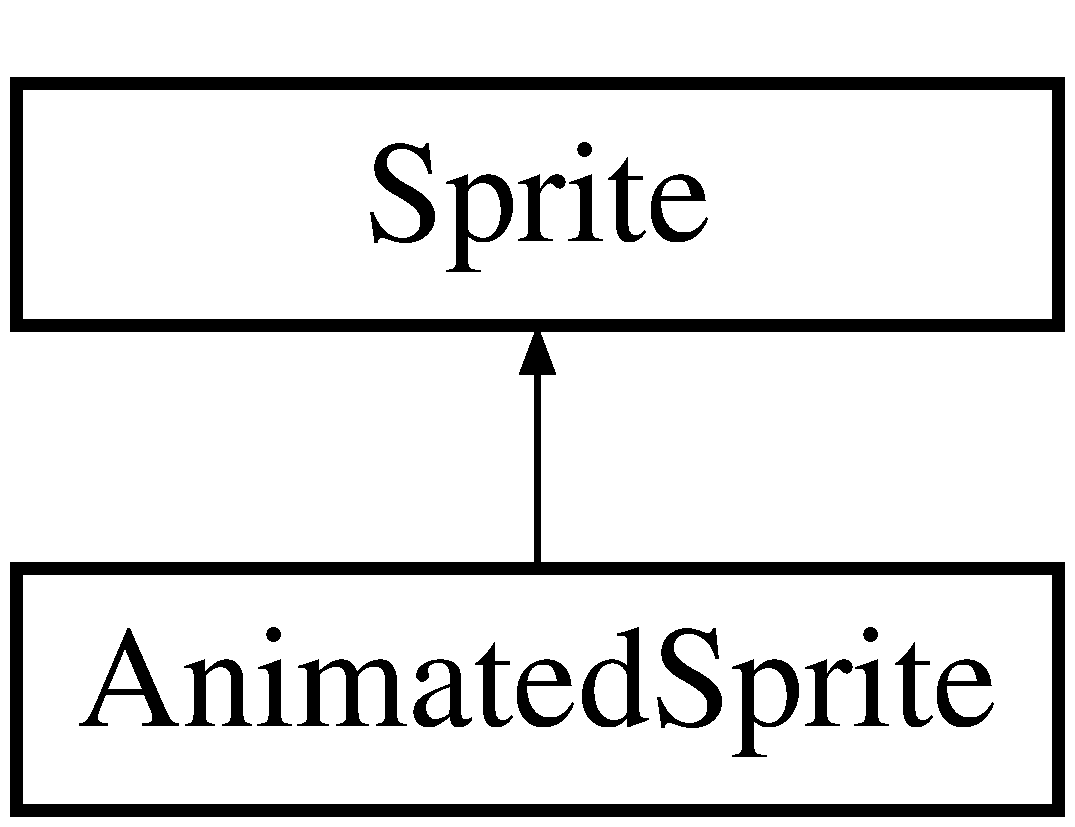
\includegraphics[height=2.000000cm]{class_sprite}
\end{center}
\end{figure}
\subsection*{Public Member Functions}
\begin{DoxyCompactItemize}
\item 
{\bf Sprite} ({\bf Graphic} \&graphics, const std\+::string \&filepath, int src\+\_\+x, int src\+\_\+y, int width, int height)
\begin{DoxyCompactList}\small\item\em Legt ein neues \doxyref{Sprite}{p.}{class_sprite} an. \end{DoxyCompactList}\item 
virtual void {\bfseries update} (int)\label{class_sprite_ae93ffca39a384237789ec65de213e68f}

\item 
void {\bf draw} ({\bf Graphic} \&graphics, int x, int y)
\begin{DoxyCompactList}\small\item\em Das \doxyref{Sprite}{p.}{class_sprite} wird auf den im graphics Objekt enthaltenen Screen gezeichnet. \end{DoxyCompactList}\end{DoxyCompactItemize}
\subsection*{Protected Attributes}
\begin{DoxyCompactItemize}
\item 
{\bf S\+D\+L\+\_\+\+Rect} {\bf src\+Rect}
\end{DoxyCompactItemize}
\subsection*{Private Attributes}
\begin{DoxyCompactItemize}
\item 
{\bf S\+D\+L\+\_\+\+Surface} $\ast$ {\bf sprite\+Sheet}
\end{DoxyCompactItemize}


\subsection{Detailed Description}
Die \doxyref{Sprite}{p.}{class_sprite} Klasse hält ein Bild, welches bei Bedarf auf den Screen gezeichnet werden kann. 

\subsection{Constructor \& Destructor Documentation}
\index{Sprite@{Sprite}!Sprite@{Sprite}}
\index{Sprite@{Sprite}!Sprite@{Sprite}}
\subsubsection[{Sprite}]{\setlength{\rightskip}{0pt plus 5cm}Sprite\+::\+Sprite (
\begin{DoxyParamCaption}
\item[{{\bf Graphic} \&}]{graphics, }
\item[{const std\+::string \&}]{filepath, }
\item[{int}]{src\+\_\+x, }
\item[{int}]{src\+\_\+y, }
\item[{int}]{width, }
\item[{int}]{height}
\end{DoxyParamCaption}
)}\label{class_sprite_a47466164808cee0827ed2fa769cc76e6}


Legt ein neues \doxyref{Sprite}{p.}{class_sprite} an. 


\begin{DoxyParams}{Parameters}
{\em graphics} & object \\
\hline
{\em filepath} & -\/ Der Dateipfad des zu ladenen Bildes \\
\hline
{\em src\+\_\+x} & -\/ Der X-\/\+Offset der auf das \doxyref{Sprite}{p.}{class_sprite} angelegt wird \\
\hline
{\em src\+\_\+y} & -\/ Der Y-\/\+Offset der auf das \doxyref{Sprite}{p.}{class_sprite} angelegt wird \\
\hline
{\em width} & -\/ Legt die Weite des Sprites fest \\
\hline
{\em height} & -\/ Legt die Höhe des Sprites fest \\
\hline
\end{DoxyParams}


\subsection{Member Function Documentation}
\index{Sprite@{Sprite}!draw@{draw}}
\index{draw@{draw}!Sprite@{Sprite}}
\subsubsection[{draw}]{\setlength{\rightskip}{0pt plus 5cm}void Sprite\+::draw (
\begin{DoxyParamCaption}
\item[{{\bf Graphic} \&}]{graphics, }
\item[{int}]{x, }
\item[{int}]{y}
\end{DoxyParamCaption}
)}\label{class_sprite_ad1a918703101e1d9e63f82da7504e024}


Das \doxyref{Sprite}{p.}{class_sprite} wird auf den im graphics Objekt enthaltenen Screen gezeichnet. 


\begin{DoxyParams}{Parameters}
{\em graphics} & -\/ Auf dieses graphic Objekt wird das \doxyref{Sprite}{p.}{class_sprite} gezeichnet \\
\hline
{\em x} & -\/ Die X-\/\+Position des Sprites auf dem Screen \\
\hline
{\em y} & -\/ Die Y-\/\+Position des Sprites auf dem Screen \\
\hline
\end{DoxyParams}


\subsection{Member Data Documentation}
\index{Sprite@{Sprite}!sprite\+Sheet@{sprite\+Sheet}}
\index{sprite\+Sheet@{sprite\+Sheet}!Sprite@{Sprite}}
\subsubsection[{sprite\+Sheet}]{\setlength{\rightskip}{0pt plus 5cm}{\bf S\+D\+L\+\_\+\+Surface}$\ast$ Sprite\+::sprite\+Sheet\hspace{0.3cm}{\ttfamily [private]}}\label{class_sprite_aa356e52e44c86d8d76cc3060eb41ae06}
Enthält das Bild \index{Sprite@{Sprite}!src\+Rect@{src\+Rect}}
\index{src\+Rect@{src\+Rect}!Sprite@{Sprite}}
\subsubsection[{src\+Rect}]{\setlength{\rightskip}{0pt plus 5cm}{\bf S\+D\+L\+\_\+\+Rect} Sprite\+::src\+Rect\hspace{0.3cm}{\ttfamily [protected]}}\label{class_sprite_a8fa271c176620b583103408ba6d95810}
Legt die Abmessungen, Höhe und Weite des Sprites fest 

The documentation for this class was generated from the following files\+:\begin{DoxyCompactItemize}
\item 
C\+:/\+Users/\+Max/\+Documents/\+Git\+Hub/\+Ballerburg/\+Ballerburg\+\_\+v001/sprite.\+h\item 
C\+:/\+Users/\+Max/\+Documents/\+Git\+Hub/\+Ballerburg/\+Ballerburg\+\_\+v001/sprite.\+cpp\end{DoxyCompactItemize}

\section{Tracer Class Reference}
\label{class_tracer}\index{Tracer@{Tracer}}
\subsection*{Public Member Functions}
\begin{DoxyCompactItemize}
\item 
{\bfseries Tracer} (const char $\ast$name)\label{class_tracer_ab5f76eb2148eb92a6da5d72c61cb5005}

\item 
{\bfseries Tracer} (std\+::string name)\label{class_tracer_a4f325d324556b69e2897d0b137b70e99}

\item 
void {\bfseries set\+Nesting\+Prefix} (const std\+::string \&prefix)\label{class_tracer_a83ec129e27aed135efaeb395f9984641}

\item 
{\footnotesize template$<$typename T $>$ }\\const {\bf Tracer} \& {\bfseries operator$<$$<$} (const T \&value) const \label{class_tracer_ad94e93b9f930cd450c4f6bb0165de306}

\end{DoxyCompactItemize}
\subsection*{Friends}
\begin{DoxyCompactItemize}
\item 
{\bf Tracer} {\bfseries trace} ()\label{class_tracer_aba74df155ca9fabb2e45947113f50944}

\end{DoxyCompactItemize}


The documentation for this class was generated from the following files\+:\begin{DoxyCompactItemize}
\item 
C\+:/\+Users/\+Max/\+Documents/\+Git\+Hub/\+Ballerburg/\+Ballerburg\+\_\+v001/tracer.\+h\item 
C\+:/\+Users/\+Max/\+Documents/\+Git\+Hub/\+Ballerburg/\+Ballerburg\+\_\+v001/tracer.\+cpp\end{DoxyCompactItemize}

\section{Uint64 Struct Reference}
\label{struct_uint64}\index{Uint64@{Uint64}}
\subsection*{Public Attributes}
\begin{DoxyCompactItemize}
\item 
Uint32 {\bfseries hi}\label{struct_uint64_aebe59cbeb37832b60d27071eca9fef3f}

\item 
Uint32 {\bfseries lo}\label{struct_uint64_a110735976529c94010e0e1ff33bcb116}

\end{DoxyCompactItemize}


The documentation for this struct was generated from the following file\+:\begin{DoxyCompactItemize}
\item 
C\+:/\+Users/\+Max/\+Documents/\+Git\+Hub/\+Ballerburg/\+Ballerburg\+\_\+v001/\+Resources/\+S\+D\+L-\/1.\+2.\+15/include/\+S\+D\+L/{\bf S\+D\+L\+\_\+stdinc.\+h}\end{DoxyCompactItemize}

\chapter{File Documentation}
\section{C\+:/\+Users/\+Max/\+Documents/\+Git\+Hub/\+Ballerburg/\+Ballerburg\+\_\+v001/\+Resources/\+S\+D\+L-\/1.2.15/include/\+S\+D\+L/begin\+\_\+code.h File Reference}
\label{begin__code_8h}\index{C\+:/\+Users/\+Max/\+Documents/\+Git\+Hub/\+Ballerburg/\+Ballerburg\+\_\+v001/\+Resources/\+S\+D\+L-\/1.\+2.\+15/include/\+S\+D\+L/begin\+\_\+code.\+h@{C\+:/\+Users/\+Max/\+Documents/\+Git\+Hub/\+Ballerburg/\+Ballerburg\+\_\+v001/\+Resources/\+S\+D\+L-\/1.\+2.\+15/include/\+S\+D\+L/begin\+\_\+code.\+h}}
\subsection*{Macros}
\begin{DoxyCompactItemize}
\item 
\#define {\bfseries \+\_\+begin\+\_\+code\+\_\+h}\label{begin__code_8h_ad8ee189cfed593708b48fa2163caaed7}

\item 
\#define {\bf D\+E\+C\+L\+S\+P\+E\+C}
\item 
\#define {\bf S\+D\+L\+C\+A\+L\+L}
\item 
\#define {\bf \+\_\+\+\_\+inline\+\_\+\+\_\+}~inline
\item 
\#define {\bf S\+D\+L\+\_\+\+I\+N\+L\+I\+N\+E\+\_\+\+O\+K\+A\+Y}
\item 
\#define {\bf N\+U\+L\+L}~((void $\ast$)0)
\end{DoxyCompactItemize}


\subsection{Detailed Description}
This file sets things up for C dynamic library function definitions, static inlined functions, and structures aligned at 4-\/byte alignment. If you don\textquotesingle{}t like ugly C preprocessor code, don\textquotesingle{}t look at this file. \+:)

This shouldn\textquotesingle{}t be nested -- included it around code only.

Force structure packing at 4 byte alignment. This is necessary if the header is included in code which has structure packing set to an alternate value, say for loading structures from disk. The packing is reset to the previous value in \doxyref{close\+\_\+code.\+h}{p.}{close__code_8h} 

\subsection{Macro Definition Documentation}
\index{begin\+\_\+code.\+h@{begin\+\_\+code.\+h}!\+\_\+\+\_\+inline\+\_\+\+\_\+@{\+\_\+\+\_\+inline\+\_\+\+\_\+}}
\index{\+\_\+\+\_\+inline\+\_\+\+\_\+@{\+\_\+\+\_\+inline\+\_\+\+\_\+}!begin\+\_\+code.\+h@{begin\+\_\+code.\+h}}
\subsubsection[{\+\_\+\+\_\+inline\+\_\+\+\_\+}]{\setlength{\rightskip}{0pt plus 5cm}\#define \+\_\+\+\_\+inline\+\_\+\+\_\+~inline}\label{begin__code_8h_a9f04218fe09e6ee659e045b2f11542ed}
If inlining isn\textquotesingle{}t supported, remove \char`\"{}\+\_\+\+\_\+inline\+\_\+\+\_\+\char`\"{}, turning static inlined functions into static functions (resulting in code bloat in all files which include the offending header files) \index{begin\+\_\+code.\+h@{begin\+\_\+code.\+h}!D\+E\+C\+L\+S\+P\+E\+C@{D\+E\+C\+L\+S\+P\+E\+C}}
\index{D\+E\+C\+L\+S\+P\+E\+C@{D\+E\+C\+L\+S\+P\+E\+C}!begin\+\_\+code.\+h@{begin\+\_\+code.\+h}}
\subsubsection[{D\+E\+C\+L\+S\+P\+E\+C}]{\setlength{\rightskip}{0pt plus 5cm}\#define D\+E\+C\+L\+S\+P\+E\+C}\label{begin__code_8h_aa4c7a931f4a968f818b2a1b10a432185}
Some compilers use a special export keyword \index{begin\+\_\+code.\+h@{begin\+\_\+code.\+h}!N\+U\+L\+L@{N\+U\+L\+L}}
\index{N\+U\+L\+L@{N\+U\+L\+L}!begin\+\_\+code.\+h@{begin\+\_\+code.\+h}}
\subsubsection[{N\+U\+L\+L}]{\setlength{\rightskip}{0pt plus 5cm}\#define N\+U\+L\+L~((void $\ast$)0)}\label{begin__code_8h_a070d2ce7b6bb7e5c05602aa8c308d0c4}
Apparently this is needed by several Windows compilers \index{begin\+\_\+code.\+h@{begin\+\_\+code.\+h}!S\+D\+L\+\_\+\+I\+N\+L\+I\+N\+E\+\_\+\+O\+K\+A\+Y@{S\+D\+L\+\_\+\+I\+N\+L\+I\+N\+E\+\_\+\+O\+K\+A\+Y}}
\index{S\+D\+L\+\_\+\+I\+N\+L\+I\+N\+E\+\_\+\+O\+K\+A\+Y@{S\+D\+L\+\_\+\+I\+N\+L\+I\+N\+E\+\_\+\+O\+K\+A\+Y}!begin\+\_\+code.\+h@{begin\+\_\+code.\+h}}
\subsubsection[{S\+D\+L\+\_\+\+I\+N\+L\+I\+N\+E\+\_\+\+O\+K\+A\+Y}]{\setlength{\rightskip}{0pt plus 5cm}\#define S\+D\+L\+\_\+\+I\+N\+L\+I\+N\+E\+\_\+\+O\+K\+A\+Y}\label{begin__code_8h_a947320556194d84f3494292a480dd3a2}
Set up compiler-\/specific options for inlining functions \index{begin\+\_\+code.\+h@{begin\+\_\+code.\+h}!S\+D\+L\+C\+A\+L\+L@{S\+D\+L\+C\+A\+L\+L}}
\index{S\+D\+L\+C\+A\+L\+L@{S\+D\+L\+C\+A\+L\+L}!begin\+\_\+code.\+h@{begin\+\_\+code.\+h}}
\subsubsection[{S\+D\+L\+C\+A\+L\+L}]{\setlength{\rightskip}{0pt plus 5cm}\#define S\+D\+L\+C\+A\+L\+L}\label{begin__code_8h_a81faf4ba0455dc75f2e0507eddb79401}
By default S\+D\+L uses the C calling convention 
\section{C\+:/\+Users/\+Max/\+Documents/\+Git\+Hub/\+Ballerburg/\+Ballerburg\+\_\+v001/\+Resources/\+S\+D\+L-\/1.2.15/include/\+S\+D\+L/close\+\_\+code.h File Reference}
\label{close__code_8h}\index{C\+:/\+Users/\+Max/\+Documents/\+Git\+Hub/\+Ballerburg/\+Ballerburg\+\_\+v001/\+Resources/\+S\+D\+L-\/1.\+2.\+15/include/\+S\+D\+L/close\+\_\+code.\+h@{C\+:/\+Users/\+Max/\+Documents/\+Git\+Hub/\+Ballerburg/\+Ballerburg\+\_\+v001/\+Resources/\+S\+D\+L-\/1.\+2.\+15/include/\+S\+D\+L/close\+\_\+code.\+h}}


This file reverses the effects of \doxyref{begin\+\_\+code.\+h}{p.}{begin__code_8h} and should be included after you finish any function and structure declarations in your headers.  




\subsection{Detailed Description}
This file reverses the effects of \doxyref{begin\+\_\+code.\+h}{p.}{begin__code_8h} and should be included after you finish any function and structure declarations in your headers. 

Reset structure packing at previous byte alignment.
\section{C\+:/\+Users/\+Max/\+Documents/\+Git\+Hub/\+Ballerburg/\+Ballerburg\+\_\+v001/\+Resources/\+S\+D\+L-\/1.2.15/include/\+S\+D\+L/\+S\+D\+L.h File Reference}
\label{_s_d_l_8h}\index{C\+:/\+Users/\+Max/\+Documents/\+Git\+Hub/\+Ballerburg/\+Ballerburg\+\_\+v001/\+Resources/\+S\+D\+L-\/1.\+2.\+15/include/\+S\+D\+L/\+S\+D\+L.\+h@{C\+:/\+Users/\+Max/\+Documents/\+Git\+Hub/\+Ballerburg/\+Ballerburg\+\_\+v001/\+Resources/\+S\+D\+L-\/1.\+2.\+15/include/\+S\+D\+L/\+S\+D\+L.\+h}}
{\ttfamily \#include \char`\"{}S\+D\+L\+\_\+main.\+h\char`\"{}}\\*
{\ttfamily \#include \char`\"{}S\+D\+L\+\_\+stdinc.\+h\char`\"{}}\\*
{\ttfamily \#include \char`\"{}S\+D\+L\+\_\+audio.\+h\char`\"{}}\\*
{\ttfamily \#include \char`\"{}S\+D\+L\+\_\+cdrom.\+h\char`\"{}}\\*
{\ttfamily \#include \char`\"{}S\+D\+L\+\_\+cpuinfo.\+h\char`\"{}}\\*
{\ttfamily \#include \char`\"{}S\+D\+L\+\_\+endian.\+h\char`\"{}}\\*
{\ttfamily \#include \char`\"{}S\+D\+L\+\_\+error.\+h\char`\"{}}\\*
{\ttfamily \#include \char`\"{}S\+D\+L\+\_\+events.\+h\char`\"{}}\\*
{\ttfamily \#include \char`\"{}S\+D\+L\+\_\+loadso.\+h\char`\"{}}\\*
{\ttfamily \#include \char`\"{}S\+D\+L\+\_\+mutex.\+h\char`\"{}}\\*
{\ttfamily \#include \char`\"{}S\+D\+L\+\_\+rwops.\+h\char`\"{}}\\*
{\ttfamily \#include \char`\"{}S\+D\+L\+\_\+thread.\+h\char`\"{}}\\*
{\ttfamily \#include \char`\"{}S\+D\+L\+\_\+timer.\+h\char`\"{}}\\*
{\ttfamily \#include \char`\"{}S\+D\+L\+\_\+video.\+h\char`\"{}}\\*
{\ttfamily \#include \char`\"{}S\+D\+L\+\_\+version.\+h\char`\"{}}\\*
{\ttfamily \#include \char`\"{}begin\+\_\+code.\+h\char`\"{}}\\*
{\ttfamily \#include \char`\"{}close\+\_\+code.\+h\char`\"{}}\\*
\subsection*{Macros}
\begin{Indent}{\bf S\+D\+L\+\_\+\+I\+N\+I\+T Flags}\par
{\em These are the flags which may be passed to \doxyref{S\+D\+L\+\_\+\+Init()}{p.}{_s_d_l_8h_a8fc8d35348d7c74bad8392d776c937b8} -- you should specify the subsystems which you will be using in your application. }\begin{DoxyCompactItemize}
\item 
\#define {\bfseries S\+D\+L\+\_\+\+I\+N\+I\+T\+\_\+\+T\+I\+M\+E\+R}~0x00000001\label{_s_d_l_8h_aadfaf3382d6e136b5944d1d5e7e50290}

\item 
\#define {\bfseries S\+D\+L\+\_\+\+I\+N\+I\+T\+\_\+\+A\+U\+D\+I\+O}~0x00000010\label{_s_d_l_8h_abeceb02c19508655cb05cc8e64206333}

\item 
\#define {\bfseries S\+D\+L\+\_\+\+I\+N\+I\+T\+\_\+\+V\+I\+D\+E\+O}~0x00000020\label{_s_d_l_8h_afc988e510ed522628ffeb7c76f80c233}

\item 
\#define {\bfseries S\+D\+L\+\_\+\+I\+N\+I\+T\+\_\+\+C\+D\+R\+O\+M}~0x00000100\label{_s_d_l_8h_a71212def1530b14bc34e6906e8ada4f1}

\item 
\#define {\bfseries S\+D\+L\+\_\+\+I\+N\+I\+T\+\_\+\+J\+O\+Y\+S\+T\+I\+C\+K}~0x00000200\label{_s_d_l_8h_ad6b47d785eaa00d9c48e6c1cff4aef4b}

\item 
\#define {\bf S\+D\+L\+\_\+\+I\+N\+I\+T\+\_\+\+N\+O\+P\+A\+R\+A\+C\+H\+U\+T\+E}~0x00100000
\item 
\#define {\bf S\+D\+L\+\_\+\+I\+N\+I\+T\+\_\+\+E\+V\+E\+N\+T\+T\+H\+R\+E\+A\+D}~0x01000000
\item 
\#define {\bfseries S\+D\+L\+\_\+\+I\+N\+I\+T\+\_\+\+E\+V\+E\+R\+Y\+T\+H\+I\+N\+G}~0x0000\+F\+F\+F\+F\label{_s_d_l_8h_a574afd93f30161d6e87449f675081fb5}

\end{DoxyCompactItemize}
\end{Indent}
\subsection*{Functions}
\begin{DoxyCompactItemize}
\item 
{\bf D\+E\+C\+L\+S\+P\+E\+C} int {\bf S\+D\+L\+C\+A\+L\+L} {\bf S\+D\+L\+\_\+\+Init} (Uint32 flags)
\item 
{\bf D\+E\+C\+L\+S\+P\+E\+C} int {\bf S\+D\+L\+C\+A\+L\+L} {\bf S\+D\+L\+\_\+\+Init\+Sub\+System} (Uint32 flags)
\item 
{\bf D\+E\+C\+L\+S\+P\+E\+C} void {\bf S\+D\+L\+C\+A\+L\+L} {\bf S\+D\+L\+\_\+\+Quit\+Sub\+System} (Uint32 flags)
\item 
{\bf D\+E\+C\+L\+S\+P\+E\+C} Uint32 {\bf S\+D\+L\+C\+A\+L\+L} {\bf S\+D\+L\+\_\+\+Was\+Init} (Uint32 flags)
\item 
{\bf D\+E\+C\+L\+S\+P\+E\+C} void {\bf S\+D\+L\+C\+A\+L\+L} {\bf S\+D\+L\+\_\+\+Quit} (void)
\end{DoxyCompactItemize}


\subsection{Detailed Description}
Main include header for the S\+D\+L library

\begin{DoxyNote}{Note}
As of version 0.\+5, S\+D\+L is loaded dynamically into the application 
\end{DoxyNote}


\subsection{Macro Definition Documentation}
\index{S\+D\+L.\+h@{S\+D\+L.\+h}!S\+D\+L\+\_\+\+I\+N\+I\+T\+\_\+\+E\+V\+E\+N\+T\+T\+H\+R\+E\+A\+D@{S\+D\+L\+\_\+\+I\+N\+I\+T\+\_\+\+E\+V\+E\+N\+T\+T\+H\+R\+E\+A\+D}}
\index{S\+D\+L\+\_\+\+I\+N\+I\+T\+\_\+\+E\+V\+E\+N\+T\+T\+H\+R\+E\+A\+D@{S\+D\+L\+\_\+\+I\+N\+I\+T\+\_\+\+E\+V\+E\+N\+T\+T\+H\+R\+E\+A\+D}!S\+D\+L.\+h@{S\+D\+L.\+h}}
\subsubsection[{S\+D\+L\+\_\+\+I\+N\+I\+T\+\_\+\+E\+V\+E\+N\+T\+T\+H\+R\+E\+A\+D}]{\setlength{\rightskip}{0pt plus 5cm}\#define S\+D\+L\+\_\+\+I\+N\+I\+T\+\_\+\+E\+V\+E\+N\+T\+T\+H\+R\+E\+A\+D~0x01000000}\label{_s_d_l_8h_aca8aae362eee073daaf9a04f80176481}
Not supported on all O\+S\textquotesingle{}s \index{S\+D\+L.\+h@{S\+D\+L.\+h}!S\+D\+L\+\_\+\+I\+N\+I\+T\+\_\+\+N\+O\+P\+A\+R\+A\+C\+H\+U\+T\+E@{S\+D\+L\+\_\+\+I\+N\+I\+T\+\_\+\+N\+O\+P\+A\+R\+A\+C\+H\+U\+T\+E}}
\index{S\+D\+L\+\_\+\+I\+N\+I\+T\+\_\+\+N\+O\+P\+A\+R\+A\+C\+H\+U\+T\+E@{S\+D\+L\+\_\+\+I\+N\+I\+T\+\_\+\+N\+O\+P\+A\+R\+A\+C\+H\+U\+T\+E}!S\+D\+L.\+h@{S\+D\+L.\+h}}
\subsubsection[{S\+D\+L\+\_\+\+I\+N\+I\+T\+\_\+\+N\+O\+P\+A\+R\+A\+C\+H\+U\+T\+E}]{\setlength{\rightskip}{0pt plus 5cm}\#define S\+D\+L\+\_\+\+I\+N\+I\+T\+\_\+\+N\+O\+P\+A\+R\+A\+C\+H\+U\+T\+E~0x00100000}\label{_s_d_l_8h_ab848174dfbc69cb2cc7bbf06a6e5c584}
Don\textquotesingle{}t catch fatal signals 

\subsection{Function Documentation}
\index{S\+D\+L.\+h@{S\+D\+L.\+h}!S\+D\+L\+\_\+\+Init@{S\+D\+L\+\_\+\+Init}}
\index{S\+D\+L\+\_\+\+Init@{S\+D\+L\+\_\+\+Init}!S\+D\+L.\+h@{S\+D\+L.\+h}}
\subsubsection[{S\+D\+L\+\_\+\+Init}]{\setlength{\rightskip}{0pt plus 5cm}{\bf D\+E\+C\+L\+S\+P\+E\+C} int {\bf S\+D\+L\+C\+A\+L\+L} S\+D\+L\+\_\+\+Init (
\begin{DoxyParamCaption}
\item[{Uint32}]{flags}
\end{DoxyParamCaption}
)}\label{_s_d_l_8h_a8fc8d35348d7c74bad8392d776c937b8}
This function loads the S\+D\+L dynamically linked library and initializes the subsystems specified by \textquotesingle{}flags\textquotesingle{} (and those satisfying dependencies) Unless the S\+D\+L\+\_\+\+I\+N\+I\+T\+\_\+\+N\+O\+P\+A\+R\+A\+C\+H\+U\+T\+E flag is set, it will install cleanup signal handlers for some commonly ignored fatal signals (like S\+I\+G\+S\+E\+G\+V) \index{S\+D\+L.\+h@{S\+D\+L.\+h}!S\+D\+L\+\_\+\+Init\+Sub\+System@{S\+D\+L\+\_\+\+Init\+Sub\+System}}
\index{S\+D\+L\+\_\+\+Init\+Sub\+System@{S\+D\+L\+\_\+\+Init\+Sub\+System}!S\+D\+L.\+h@{S\+D\+L.\+h}}
\subsubsection[{S\+D\+L\+\_\+\+Init\+Sub\+System}]{\setlength{\rightskip}{0pt plus 5cm}{\bf D\+E\+C\+L\+S\+P\+E\+C} int {\bf S\+D\+L\+C\+A\+L\+L} S\+D\+L\+\_\+\+Init\+Sub\+System (
\begin{DoxyParamCaption}
\item[{Uint32}]{flags}
\end{DoxyParamCaption}
)}\label{_s_d_l_8h_adfbfddc0ec609b5e5e5cb1c89298e4db}
This function initializes specific S\+D\+L subsystems \index{S\+D\+L.\+h@{S\+D\+L.\+h}!S\+D\+L\+\_\+\+Quit@{S\+D\+L\+\_\+\+Quit}}
\index{S\+D\+L\+\_\+\+Quit@{S\+D\+L\+\_\+\+Quit}!S\+D\+L.\+h@{S\+D\+L.\+h}}
\subsubsection[{S\+D\+L\+\_\+\+Quit}]{\setlength{\rightskip}{0pt plus 5cm}{\bf D\+E\+C\+L\+S\+P\+E\+C} void {\bf S\+D\+L\+C\+A\+L\+L} S\+D\+L\+\_\+\+Quit (
\begin{DoxyParamCaption}
\item[{void}]{}
\end{DoxyParamCaption}
)}\label{_s_d_l_8h_afdabaf714781099083592051f2d9ac11}
This function cleans up all initialized subsystems and unloads the dynamically linked library. You should call it upon all exit conditions. \index{S\+D\+L.\+h@{S\+D\+L.\+h}!S\+D\+L\+\_\+\+Quit\+Sub\+System@{S\+D\+L\+\_\+\+Quit\+Sub\+System}}
\index{S\+D\+L\+\_\+\+Quit\+Sub\+System@{S\+D\+L\+\_\+\+Quit\+Sub\+System}!S\+D\+L.\+h@{S\+D\+L.\+h}}
\subsubsection[{S\+D\+L\+\_\+\+Quit\+Sub\+System}]{\setlength{\rightskip}{0pt plus 5cm}{\bf D\+E\+C\+L\+S\+P\+E\+C} void {\bf S\+D\+L\+C\+A\+L\+L} S\+D\+L\+\_\+\+Quit\+Sub\+System (
\begin{DoxyParamCaption}
\item[{Uint32}]{flags}
\end{DoxyParamCaption}
)}\label{_s_d_l_8h_a14e9091982e09097985e10e3ca65debb}
This function cleans up specific S\+D\+L subsystems \index{S\+D\+L.\+h@{S\+D\+L.\+h}!S\+D\+L\+\_\+\+Was\+Init@{S\+D\+L\+\_\+\+Was\+Init}}
\index{S\+D\+L\+\_\+\+Was\+Init@{S\+D\+L\+\_\+\+Was\+Init}!S\+D\+L.\+h@{S\+D\+L.\+h}}
\subsubsection[{S\+D\+L\+\_\+\+Was\+Init}]{\setlength{\rightskip}{0pt plus 5cm}{\bf D\+E\+C\+L\+S\+P\+E\+C} Uint32 {\bf S\+D\+L\+C\+A\+L\+L} S\+D\+L\+\_\+\+Was\+Init (
\begin{DoxyParamCaption}
\item[{Uint32}]{flags}
\end{DoxyParamCaption}
)}\label{_s_d_l_8h_a04dc570990c697eed95681216801710d}
This function returns mask of the specified subsystems which have been initialized. If \textquotesingle{}flags\textquotesingle{} is 0, it returns a mask of all initialized subsystems. 
\section{C\+:/\+Users/\+Max/\+Documents/\+Git\+Hub/\+Ballerburg/\+Ballerburg\+\_\+v001/\+Resources/\+S\+D\+L-\/1.2.15/include/\+S\+D\+L/\+S\+D\+L\+\_\+active.h File Reference}
\label{_s_d_l__active_8h}\index{C\+:/\+Users/\+Max/\+Documents/\+Git\+Hub/\+Ballerburg/\+Ballerburg\+\_\+v001/\+Resources/\+S\+D\+L-\/1.\+2.\+15/include/\+S\+D\+L/\+S\+D\+L\+\_\+active.\+h@{C\+:/\+Users/\+Max/\+Documents/\+Git\+Hub/\+Ballerburg/\+Ballerburg\+\_\+v001/\+Resources/\+S\+D\+L-\/1.\+2.\+15/include/\+S\+D\+L/\+S\+D\+L\+\_\+active.\+h}}


Include file for S\+D\+L application focus event handling.  


{\ttfamily \#include \char`\"{}S\+D\+L\+\_\+stdinc.\+h\char`\"{}}\\*
{\ttfamily \#include \char`\"{}S\+D\+L\+\_\+error.\+h\char`\"{}}\\*
{\ttfamily \#include \char`\"{}begin\+\_\+code.\+h\char`\"{}}\\*
{\ttfamily \#include \char`\"{}close\+\_\+code.\+h\char`\"{}}\\*
\subsection*{Macros}
\begin{Indent}{\bf The available application states}\par
\begin{DoxyCompactItemize}
\item 
\#define {\bf S\+D\+L\+\_\+\+A\+P\+P\+M\+O\+U\+S\+E\+F\+O\+C\+U\+S}~0x01\label{_s_d_l__active_8h_adbb0da5a3196e16a2104a8dd4d048177}

\begin{DoxyCompactList}\small\item\em The app has mouse coverage. \end{DoxyCompactList}\item 
\#define {\bf S\+D\+L\+\_\+\+A\+P\+P\+I\+N\+P\+U\+T\+F\+O\+C\+U\+S}~0x02\label{_s_d_l__active_8h_ac41cbb6cae92292898f29b6e6338d5a6}

\begin{DoxyCompactList}\small\item\em The app has input focus. \end{DoxyCompactList}\item 
\#define {\bf S\+D\+L\+\_\+\+A\+P\+P\+A\+C\+T\+I\+V\+E}~0x04\label{_s_d_l__active_8h_a54820fe5c98fa3369dfad1f13c76cb4f}

\begin{DoxyCompactList}\small\item\em The application is active. \end{DoxyCompactList}\end{DoxyCompactItemize}
\end{Indent}
\subsection*{Functions}
\begin{DoxyCompactItemize}
\item 
{\bf D\+E\+C\+L\+S\+P\+E\+C} Uint8 {\bf S\+D\+L\+C\+A\+L\+L} {\bf S\+D\+L\+\_\+\+Get\+App\+State} (void)
\begin{DoxyCompactList}\small\item\em This function returns the current state of the application, which is a bitwise combination of S\+D\+L\+\_\+\+A\+P\+P\+M\+O\+U\+S\+E\+F\+O\+C\+U\+S, S\+D\+L\+\_\+\+A\+P\+P\+I\+N\+P\+U\+T\+F\+O\+C\+U\+S, and S\+D\+L\+\_\+\+A\+P\+P\+A\+C\+T\+I\+V\+E. \end{DoxyCompactList}\end{DoxyCompactItemize}


\subsection{Detailed Description}
Include file for S\+D\+L application focus event handling. 



\subsection{Function Documentation}
\index{S\+D\+L\+\_\+active.\+h@{S\+D\+L\+\_\+active.\+h}!S\+D\+L\+\_\+\+Get\+App\+State@{S\+D\+L\+\_\+\+Get\+App\+State}}
\index{S\+D\+L\+\_\+\+Get\+App\+State@{S\+D\+L\+\_\+\+Get\+App\+State}!S\+D\+L\+\_\+active.\+h@{S\+D\+L\+\_\+active.\+h}}
\subsubsection[{S\+D\+L\+\_\+\+Get\+App\+State}]{\setlength{\rightskip}{0pt plus 5cm}{\bf D\+E\+C\+L\+S\+P\+E\+C} Uint8 {\bf S\+D\+L\+C\+A\+L\+L} S\+D\+L\+\_\+\+Get\+App\+State (
\begin{DoxyParamCaption}
\item[{void}]{}
\end{DoxyParamCaption}
)}\label{_s_d_l__active_8h_a33e36b26e1d6c532e4a325188473a104}


This function returns the current state of the application, which is a bitwise combination of S\+D\+L\+\_\+\+A\+P\+P\+M\+O\+U\+S\+E\+F\+O\+C\+U\+S, S\+D\+L\+\_\+\+A\+P\+P\+I\+N\+P\+U\+T\+F\+O\+C\+U\+S, and S\+D\+L\+\_\+\+A\+P\+P\+A\+C\+T\+I\+V\+E. 

If S\+D\+L\+\_\+\+A\+P\+P\+A\+C\+T\+I\+V\+E is set, then the user is able to see your application, otherwise it has been iconified or disabled. 
\section{C\+:/\+Users/\+Max/\+Documents/\+Git\+Hub/\+Ballerburg/\+Ballerburg\+\_\+v001/\+Resources/\+S\+D\+L-\/1.2.15/include/\+S\+D\+L/\+S\+D\+L\+\_\+audio.h File Reference}
\label{_s_d_l__audio_8h}\index{C\+:/\+Users/\+Max/\+Documents/\+Git\+Hub/\+Ballerburg/\+Ballerburg\+\_\+v001/\+Resources/\+S\+D\+L-\/1.\+2.\+15/include/\+S\+D\+L/\+S\+D\+L\+\_\+audio.\+h@{C\+:/\+Users/\+Max/\+Documents/\+Git\+Hub/\+Ballerburg/\+Ballerburg\+\_\+v001/\+Resources/\+S\+D\+L-\/1.\+2.\+15/include/\+S\+D\+L/\+S\+D\+L\+\_\+audio.\+h}}
{\ttfamily \#include \char`\"{}S\+D\+L\+\_\+stdinc.\+h\char`\"{}}\\*
{\ttfamily \#include \char`\"{}S\+D\+L\+\_\+error.\+h\char`\"{}}\\*
{\ttfamily \#include \char`\"{}S\+D\+L\+\_\+endian.\+h\char`\"{}}\\*
{\ttfamily \#include \char`\"{}S\+D\+L\+\_\+mutex.\+h\char`\"{}}\\*
{\ttfamily \#include \char`\"{}S\+D\+L\+\_\+thread.\+h\char`\"{}}\\*
{\ttfamily \#include \char`\"{}S\+D\+L\+\_\+rwops.\+h\char`\"{}}\\*
{\ttfamily \#include \char`\"{}begin\+\_\+code.\+h\char`\"{}}\\*
{\ttfamily \#include \char`\"{}close\+\_\+code.\+h\char`\"{}}\\*
\subsection*{Classes}
\begin{DoxyCompactItemize}
\item 
struct {\bf S\+D\+L\+\_\+\+Audio\+Spec}
\item 
struct {\bf S\+D\+L\+\_\+\+Audio\+C\+V\+T}
\end{DoxyCompactItemize}
\subsection*{Macros}
\begin{DoxyCompactItemize}
\item 
\#define {\bf S\+D\+L\+\_\+\+Load\+W\+A\+V}(file,  spec,  audio\+\_\+buf,  audio\+\_\+len)~{\bf S\+D\+L\+\_\+\+Load\+W\+A\+V\+\_\+\+R\+W}(S\+D\+L\+\_\+\+R\+W\+From\+File(file, \char`\"{}rb\char`\"{}),1, spec,audio\+\_\+buf,audio\+\_\+len)
\item 
\#define {\bfseries S\+D\+L\+\_\+\+M\+I\+X\+\_\+\+M\+A\+X\+V\+O\+L\+U\+M\+E}~128\label{_s_d_l__audio_8h_afa8e5e92d4424b0c599e7c813c91f720}

\end{DoxyCompactItemize}
\begin{Indent}{\bf Audio format flags}\par
{\em defaults to L\+S\+B byte order }\begin{DoxyCompactItemize}
\item 
\#define {\bf A\+U\+D\+I\+O\+\_\+\+U8}~0x0008
\item 
\#define {\bf A\+U\+D\+I\+O\+\_\+\+S8}~0x8008
\item 
\#define {\bf A\+U\+D\+I\+O\+\_\+\+U16\+L\+S\+B}~0x0010
\item 
\#define {\bf A\+U\+D\+I\+O\+\_\+\+S16\+L\+S\+B}~0x8010
\item 
\#define {\bf A\+U\+D\+I\+O\+\_\+\+U16\+M\+S\+B}~0x1010
\item 
\#define {\bf A\+U\+D\+I\+O\+\_\+\+S16\+M\+S\+B}~0x9010
\item 
\#define {\bfseries A\+U\+D\+I\+O\+\_\+\+U16}~{\bf A\+U\+D\+I\+O\+\_\+\+U16\+L\+S\+B}\label{_s_d_l__audio_8h_adee2cdf7dbda44620da17cd58ca819ea}

\item 
\#define {\bfseries A\+U\+D\+I\+O\+\_\+\+S16}~{\bf A\+U\+D\+I\+O\+\_\+\+S16\+L\+S\+B}\label{_s_d_l__audio_8h_a4f4950d8eee757ebed84e50fb9316b12}

\end{DoxyCompactItemize}
\end{Indent}
\begin{Indent}{\bf Native audio byte ordering}\par
\begin{DoxyCompactItemize}
\item 
\#define {\bfseries A\+U\+D\+I\+O\+\_\+\+U16\+S\+Y\+S}~{\bf A\+U\+D\+I\+O\+\_\+\+U16\+L\+S\+B}\label{_s_d_l__audio_8h_afafc9f93ee2c583130c4152e243ba5b8}

\item 
\#define {\bfseries A\+U\+D\+I\+O\+\_\+\+S16\+S\+Y\+S}~{\bf A\+U\+D\+I\+O\+\_\+\+S16\+L\+S\+B}\label{_s_d_l__audio_8h_a4722de7e16982dd078f2b8cc64b9bae7}

\end{DoxyCompactItemize}
\end{Indent}
\subsection*{Typedefs}
\begin{DoxyCompactItemize}
\item 
typedef struct {\bf S\+D\+L\+\_\+\+Audio\+Spec} {\bf S\+D\+L\+\_\+\+Audio\+Spec}
\item 
typedef struct {\bf S\+D\+L\+\_\+\+Audio\+C\+V\+T} {\bf S\+D\+L\+\_\+\+Audio\+C\+V\+T}
\end{DoxyCompactItemize}
\subsection*{Enumerations}
\begin{DoxyCompactItemize}
\item 
enum {\bfseries S\+D\+L\+\_\+audiostatus} \{ {\bfseries S\+D\+L\+\_\+\+A\+U\+D\+I\+O\+\_\+\+S\+T\+O\+P\+P\+E\+D} = 0, 
{\bfseries S\+D\+L\+\_\+\+A\+U\+D\+I\+O\+\_\+\+P\+L\+A\+Y\+I\+N\+G}, 
{\bfseries S\+D\+L\+\_\+\+A\+U\+D\+I\+O\+\_\+\+P\+A\+U\+S\+E\+D}
 \}\label{_s_d_l__audio_8h_ae67ea72fc0b72d474bdaaf42b1dd9361}

\end{DoxyCompactItemize}
\subsection*{Functions}
\begin{DoxyCompactItemize}
\item 
{\bf D\+E\+C\+L\+S\+P\+E\+C} char $\ast${\bf S\+D\+L\+C\+A\+L\+L} {\bf S\+D\+L\+\_\+\+Audio\+Driver\+Name} (char $\ast$namebuf, int maxlen)
\item 
{\bf D\+E\+C\+L\+S\+P\+E\+C} int {\bf S\+D\+L\+C\+A\+L\+L} {\bf S\+D\+L\+\_\+\+Open\+Audio} ({\bf S\+D\+L\+\_\+\+Audio\+Spec} $\ast$desired, {\bf S\+D\+L\+\_\+\+Audio\+Spec} $\ast$obtained)
\item 
{\bf D\+E\+C\+L\+S\+P\+E\+C} S\+D\+L\+\_\+audiostatus {\bf S\+D\+L\+C\+A\+L\+L} {\bf S\+D\+L\+\_\+\+Get\+Audio\+Status} (void)
\item 
{\bf D\+E\+C\+L\+S\+P\+E\+C} void {\bf S\+D\+L\+C\+A\+L\+L} {\bf S\+D\+L\+\_\+\+Pause\+Audio} (int pause\+\_\+on)
\item 
{\bf D\+E\+C\+L\+S\+P\+E\+C} {\bf S\+D\+L\+\_\+\+Audio\+Spec} $\ast${\bf S\+D\+L\+C\+A\+L\+L} {\bf S\+D\+L\+\_\+\+Load\+W\+A\+V\+\_\+\+R\+W} ({\bf S\+D\+L\+\_\+\+R\+Wops} $\ast$src, int freesrc, {\bf S\+D\+L\+\_\+\+Audio\+Spec} $\ast$spec, Uint8 $\ast$$\ast$audio\+\_\+buf, Uint32 $\ast$audio\+\_\+len)
\item 
{\bf D\+E\+C\+L\+S\+P\+E\+C} void {\bf S\+D\+L\+C\+A\+L\+L} {\bf S\+D\+L\+\_\+\+Free\+W\+A\+V} (Uint8 $\ast$audio\+\_\+buf)
\item 
{\bf D\+E\+C\+L\+S\+P\+E\+C} int {\bf S\+D\+L\+C\+A\+L\+L} {\bf S\+D\+L\+\_\+\+Build\+Audio\+C\+V\+T} ({\bf S\+D\+L\+\_\+\+Audio\+C\+V\+T} $\ast$cvt, Uint16 src\+\_\+format, Uint8 src\+\_\+channels, int src\+\_\+rate, Uint16 dst\+\_\+format, Uint8 dst\+\_\+channels, int dst\+\_\+rate)
\item 
{\bf D\+E\+C\+L\+S\+P\+E\+C} int {\bf S\+D\+L\+C\+A\+L\+L} {\bf S\+D\+L\+\_\+\+Convert\+Audio} ({\bf S\+D\+L\+\_\+\+Audio\+C\+V\+T} $\ast$cvt)
\item 
{\bf D\+E\+C\+L\+S\+P\+E\+C} void {\bf S\+D\+L\+C\+A\+L\+L} {\bf S\+D\+L\+\_\+\+Mix\+Audio} (Uint8 $\ast$dst, const Uint8 $\ast$src, Uint32 len, int volume)
\item 
{\bf D\+E\+C\+L\+S\+P\+E\+C} void {\bf S\+D\+L\+C\+A\+L\+L} {\bf S\+D\+L\+\_\+\+Close\+Audio} (void)
\end{DoxyCompactItemize}
\begin{Indent}{\bf Audio Init and Quit}\par
{\em These functions are used internally, and should not be used unless you have a specific need to specify the audio driver you want to use. You should normally use \doxyref{S\+D\+L\+\_\+\+Init()}{p.}{_s_d_l_8h_a8fc8d35348d7c74bad8392d776c937b8} or \doxyref{S\+D\+L\+\_\+\+Init\+Sub\+System()}{p.}{_s_d_l_8h_adfbfddc0ec609b5e5e5cb1c89298e4db}. }\begin{DoxyCompactItemize}
\item 
{\bf D\+E\+C\+L\+S\+P\+E\+C} int {\bf S\+D\+L\+C\+A\+L\+L} {\bfseries S\+D\+L\+\_\+\+Audio\+Init} (const char $\ast$driver\+\_\+name)\label{_s_d_l__audio_8h_ae3667d6ba706a3ca7affd8611632fa2c}

\item 
{\bf D\+E\+C\+L\+S\+P\+E\+C} void {\bf S\+D\+L\+C\+A\+L\+L} {\bfseries S\+D\+L\+\_\+\+Audio\+Quit} (void)\label{_s_d_l__audio_8h_a478c602cbfaab8663cb4f58a62600323}

\end{DoxyCompactItemize}
\end{Indent}
\begin{Indent}{\bf Audio Locks}\par
{\em The lock manipulated by these functions protects the callback function. During a Lock\+Audio/\+Unlock\+Audio pair, you can be guaranteed that the callback function is not running. Do not call these from the callback function or you will cause deadlock. }\begin{DoxyCompactItemize}
\item 
{\bf D\+E\+C\+L\+S\+P\+E\+C} void {\bf S\+D\+L\+C\+A\+L\+L} {\bfseries S\+D\+L\+\_\+\+Lock\+Audio} (void)\label{_s_d_l__audio_8h_a7ffa484f230f6085e271a4f43e678f06}

\item 
{\bf D\+E\+C\+L\+S\+P\+E\+C} void {\bf S\+D\+L\+C\+A\+L\+L} {\bfseries S\+D\+L\+\_\+\+Unlock\+Audio} (void)\label{_s_d_l__audio_8h_a76d8179bee14dad268e65378058d897d}

\end{DoxyCompactItemize}
\end{Indent}


\subsection{Detailed Description}
Access to the raw audio mixing buffer for the S\+D\+L library 

\subsection{Macro Definition Documentation}
\index{S\+D\+L\+\_\+audio.\+h@{S\+D\+L\+\_\+audio.\+h}!A\+U\+D\+I\+O\+\_\+\+S16\+L\+S\+B@{A\+U\+D\+I\+O\+\_\+\+S16\+L\+S\+B}}
\index{A\+U\+D\+I\+O\+\_\+\+S16\+L\+S\+B@{A\+U\+D\+I\+O\+\_\+\+S16\+L\+S\+B}!S\+D\+L\+\_\+audio.\+h@{S\+D\+L\+\_\+audio.\+h}}
\subsubsection[{A\+U\+D\+I\+O\+\_\+\+S16\+L\+S\+B}]{\setlength{\rightskip}{0pt plus 5cm}\#define A\+U\+D\+I\+O\+\_\+\+S16\+L\+S\+B~0x8010}\label{_s_d_l__audio_8h_a23838d612e88ce72d82c3e51460f831b}
Signed 16-\/bit samples \index{S\+D\+L\+\_\+audio.\+h@{S\+D\+L\+\_\+audio.\+h}!A\+U\+D\+I\+O\+\_\+\+S16\+M\+S\+B@{A\+U\+D\+I\+O\+\_\+\+S16\+M\+S\+B}}
\index{A\+U\+D\+I\+O\+\_\+\+S16\+M\+S\+B@{A\+U\+D\+I\+O\+\_\+\+S16\+M\+S\+B}!S\+D\+L\+\_\+audio.\+h@{S\+D\+L\+\_\+audio.\+h}}
\subsubsection[{A\+U\+D\+I\+O\+\_\+\+S16\+M\+S\+B}]{\setlength{\rightskip}{0pt plus 5cm}\#define A\+U\+D\+I\+O\+\_\+\+S16\+M\+S\+B~0x9010}\label{_s_d_l__audio_8h_a3109dfb1d7aab29dff2b62d630e690ca}
As above, but big-\/endian byte order \index{S\+D\+L\+\_\+audio.\+h@{S\+D\+L\+\_\+audio.\+h}!A\+U\+D\+I\+O\+\_\+\+S8@{A\+U\+D\+I\+O\+\_\+\+S8}}
\index{A\+U\+D\+I\+O\+\_\+\+S8@{A\+U\+D\+I\+O\+\_\+\+S8}!S\+D\+L\+\_\+audio.\+h@{S\+D\+L\+\_\+audio.\+h}}
\subsubsection[{A\+U\+D\+I\+O\+\_\+\+S8}]{\setlength{\rightskip}{0pt plus 5cm}\#define A\+U\+D\+I\+O\+\_\+\+S8~0x8008}\label{_s_d_l__audio_8h_a883b3d4539451e49bf014dde0f9cca29}
Signed 8-\/bit samples \index{S\+D\+L\+\_\+audio.\+h@{S\+D\+L\+\_\+audio.\+h}!A\+U\+D\+I\+O\+\_\+\+U16\+L\+S\+B@{A\+U\+D\+I\+O\+\_\+\+U16\+L\+S\+B}}
\index{A\+U\+D\+I\+O\+\_\+\+U16\+L\+S\+B@{A\+U\+D\+I\+O\+\_\+\+U16\+L\+S\+B}!S\+D\+L\+\_\+audio.\+h@{S\+D\+L\+\_\+audio.\+h}}
\subsubsection[{A\+U\+D\+I\+O\+\_\+\+U16\+L\+S\+B}]{\setlength{\rightskip}{0pt plus 5cm}\#define A\+U\+D\+I\+O\+\_\+\+U16\+L\+S\+B~0x0010}\label{_s_d_l__audio_8h_a06808f806896c4d211314990c354b7fc}
Unsigned 16-\/bit samples \index{S\+D\+L\+\_\+audio.\+h@{S\+D\+L\+\_\+audio.\+h}!A\+U\+D\+I\+O\+\_\+\+U16\+M\+S\+B@{A\+U\+D\+I\+O\+\_\+\+U16\+M\+S\+B}}
\index{A\+U\+D\+I\+O\+\_\+\+U16\+M\+S\+B@{A\+U\+D\+I\+O\+\_\+\+U16\+M\+S\+B}!S\+D\+L\+\_\+audio.\+h@{S\+D\+L\+\_\+audio.\+h}}
\subsubsection[{A\+U\+D\+I\+O\+\_\+\+U16\+M\+S\+B}]{\setlength{\rightskip}{0pt plus 5cm}\#define A\+U\+D\+I\+O\+\_\+\+U16\+M\+S\+B~0x1010}\label{_s_d_l__audio_8h_a3b8052d0c49d14a2e3edf08eade52d3a}
As above, but big-\/endian byte order \index{S\+D\+L\+\_\+audio.\+h@{S\+D\+L\+\_\+audio.\+h}!A\+U\+D\+I\+O\+\_\+\+U8@{A\+U\+D\+I\+O\+\_\+\+U8}}
\index{A\+U\+D\+I\+O\+\_\+\+U8@{A\+U\+D\+I\+O\+\_\+\+U8}!S\+D\+L\+\_\+audio.\+h@{S\+D\+L\+\_\+audio.\+h}}
\subsubsection[{A\+U\+D\+I\+O\+\_\+\+U8}]{\setlength{\rightskip}{0pt plus 5cm}\#define A\+U\+D\+I\+O\+\_\+\+U8~0x0008}\label{_s_d_l__audio_8h_a6468b4b3fc53ada655eca866e491d75f}
Unsigned 8-\/bit samples \index{S\+D\+L\+\_\+audio.\+h@{S\+D\+L\+\_\+audio.\+h}!S\+D\+L\+\_\+\+Load\+W\+A\+V@{S\+D\+L\+\_\+\+Load\+W\+A\+V}}
\index{S\+D\+L\+\_\+\+Load\+W\+A\+V@{S\+D\+L\+\_\+\+Load\+W\+A\+V}!S\+D\+L\+\_\+audio.\+h@{S\+D\+L\+\_\+audio.\+h}}
\subsubsection[{S\+D\+L\+\_\+\+Load\+W\+A\+V}]{\setlength{\rightskip}{0pt plus 5cm}\#define S\+D\+L\+\_\+\+Load\+W\+A\+V(
\begin{DoxyParamCaption}
\item[{}]{file, }
\item[{}]{spec, }
\item[{}]{audio\+\_\+buf, }
\item[{}]{audio\+\_\+len}
\end{DoxyParamCaption}
)~{\bf S\+D\+L\+\_\+\+Load\+W\+A\+V\+\_\+\+R\+W}(S\+D\+L\+\_\+\+R\+W\+From\+File(file, \char`\"{}rb\char`\"{}),1, spec,audio\+\_\+buf,audio\+\_\+len)}\label{_s_d_l__audio_8h_a611f76dc30ba9891239bcce3f9b472b5}
Compatibility convenience function -- loads a W\+A\+V from a file 

\subsection{Typedef Documentation}
\index{S\+D\+L\+\_\+audio.\+h@{S\+D\+L\+\_\+audio.\+h}!S\+D\+L\+\_\+\+Audio\+C\+V\+T@{S\+D\+L\+\_\+\+Audio\+C\+V\+T}}
\index{S\+D\+L\+\_\+\+Audio\+C\+V\+T@{S\+D\+L\+\_\+\+Audio\+C\+V\+T}!S\+D\+L\+\_\+audio.\+h@{S\+D\+L\+\_\+audio.\+h}}
\subsubsection[{S\+D\+L\+\_\+\+Audio\+C\+V\+T}]{\setlength{\rightskip}{0pt plus 5cm}typedef struct {\bf S\+D\+L\+\_\+\+Audio\+C\+V\+T}  {\bf S\+D\+L\+\_\+\+Audio\+C\+V\+T}}\label{_s_d_l__audio_8h_acddd16bc3257a83299e7abe6d160ba0a}
A structure to hold a set of audio conversion filters and buffers \index{S\+D\+L\+\_\+audio.\+h@{S\+D\+L\+\_\+audio.\+h}!S\+D\+L\+\_\+\+Audio\+Spec@{S\+D\+L\+\_\+\+Audio\+Spec}}
\index{S\+D\+L\+\_\+\+Audio\+Spec@{S\+D\+L\+\_\+\+Audio\+Spec}!S\+D\+L\+\_\+audio.\+h@{S\+D\+L\+\_\+audio.\+h}}
\subsubsection[{S\+D\+L\+\_\+\+Audio\+Spec}]{\setlength{\rightskip}{0pt plus 5cm}typedef struct {\bf S\+D\+L\+\_\+\+Audio\+Spec}  {\bf S\+D\+L\+\_\+\+Audio\+Spec}}\label{_s_d_l__audio_8h_a77faa7fe3d22c03ee61466a901c22a25}
When filling in the desired audio spec structure,
\begin{DoxyItemize}
\item \textquotesingle{}desired-\/$>$freq\textquotesingle{} should be the desired audio frequency in samples-\/per-\/second.
\item \textquotesingle{}desired-\/$>$format\textquotesingle{} should be the desired audio format.
\item \textquotesingle{}desired-\/$>$samples\textquotesingle{} is the desired size of the audio buffer, in samples. This number should be a power of two, and may be adjusted by the audio driver to a value more suitable for the hardware. Good values seem to range between 512 and 8096 inclusive, depending on the application and C\+P\+U speed. Smaller values yield faster response time, but can lead to underflow if the application is doing heavy processing and cannot fill the audio buffer in time. A stereo sample consists of both right and left channels in L\+R ordering. Note that the number of samples is directly related to time by the following formula\+: ms = (samples$\ast$1000)/freq
\item \textquotesingle{}desired-\/$>$size\textquotesingle{} is the size in bytes of the audio buffer, and is calculated by \doxyref{S\+D\+L\+\_\+\+Open\+Audio()}{p.}{_s_d_l__audio_8h_a2edf30e7747584e28041b4986f89f440}.
\item \textquotesingle{}desired-\/$>$silence\textquotesingle{} is the value used to set the buffer to silence, and is calculated by \doxyref{S\+D\+L\+\_\+\+Open\+Audio()}{p.}{_s_d_l__audio_8h_a2edf30e7747584e28041b4986f89f440}.
\item \textquotesingle{}desired-\/$>$callback\textquotesingle{} should be set to a function that will be called when the audio device is ready for more data. It is passed a pointer to the audio buffer, and the length in bytes of the audio buffer. This function usually runs in a separate thread, and so you should protect data structures that it accesses by calling S\+D\+L\+\_\+\+Lock\+Audio() and S\+D\+L\+\_\+\+Unlock\+Audio() in your code.
\item \textquotesingle{}desired-\/$>$userdata\textquotesingle{} is passed as the first parameter to your callback function.
\end{DoxyItemize}

\begin{DoxyNote}{Note}
The calculated values in this structure are calculated by \doxyref{S\+D\+L\+\_\+\+Open\+Audio()}{p.}{_s_d_l__audio_8h_a2edf30e7747584e28041b4986f89f440} 
\end{DoxyNote}


\subsection{Function Documentation}
\index{S\+D\+L\+\_\+audio.\+h@{S\+D\+L\+\_\+audio.\+h}!S\+D\+L\+\_\+\+Audio\+Driver\+Name@{S\+D\+L\+\_\+\+Audio\+Driver\+Name}}
\index{S\+D\+L\+\_\+\+Audio\+Driver\+Name@{S\+D\+L\+\_\+\+Audio\+Driver\+Name}!S\+D\+L\+\_\+audio.\+h@{S\+D\+L\+\_\+audio.\+h}}
\subsubsection[{S\+D\+L\+\_\+\+Audio\+Driver\+Name}]{\setlength{\rightskip}{0pt plus 5cm}{\bf D\+E\+C\+L\+S\+P\+E\+C} char$\ast$ {\bf S\+D\+L\+C\+A\+L\+L} S\+D\+L\+\_\+\+Audio\+Driver\+Name (
\begin{DoxyParamCaption}
\item[{char $\ast$}]{namebuf, }
\item[{int}]{maxlen}
\end{DoxyParamCaption}
)}\label{_s_d_l__audio_8h_a1e676f8703a36ade7e3524eadfdc5dd0}
This function fills the given character buffer with the name of the current audio driver, and returns a pointer to it if the audio driver has been initialized. It returns N\+U\+L\+L if no driver has been initialized. \index{S\+D\+L\+\_\+audio.\+h@{S\+D\+L\+\_\+audio.\+h}!S\+D\+L\+\_\+\+Build\+Audio\+C\+V\+T@{S\+D\+L\+\_\+\+Build\+Audio\+C\+V\+T}}
\index{S\+D\+L\+\_\+\+Build\+Audio\+C\+V\+T@{S\+D\+L\+\_\+\+Build\+Audio\+C\+V\+T}!S\+D\+L\+\_\+audio.\+h@{S\+D\+L\+\_\+audio.\+h}}
\subsubsection[{S\+D\+L\+\_\+\+Build\+Audio\+C\+V\+T}]{\setlength{\rightskip}{0pt plus 5cm}{\bf D\+E\+C\+L\+S\+P\+E\+C} int {\bf S\+D\+L\+C\+A\+L\+L} S\+D\+L\+\_\+\+Build\+Audio\+C\+V\+T (
\begin{DoxyParamCaption}
\item[{{\bf S\+D\+L\+\_\+\+Audio\+C\+V\+T} $\ast$}]{cvt, }
\item[{Uint16}]{src\+\_\+format, }
\item[{Uint8}]{src\+\_\+channels, }
\item[{int}]{src\+\_\+rate, }
\item[{Uint16}]{dst\+\_\+format, }
\item[{Uint8}]{dst\+\_\+channels, }
\item[{int}]{dst\+\_\+rate}
\end{DoxyParamCaption}
)}\label{_s_d_l__audio_8h_ab89d6be44de5fbe6d06fe59e05975e68}
This function takes a source format and rate and a destination format and rate, and initializes the \textquotesingle{}cvt\textquotesingle{} structure with information needed by \doxyref{S\+D\+L\+\_\+\+Convert\+Audio()}{p.}{_s_d_l__audio_8h_a8e8660222356e07002dde4928118b7df} to convert a buffer of audio data from one format to the other.

\begin{DoxyReturn}{Returns}
This function returns 0, or -\/1 if there was an error. 
\end{DoxyReturn}
\index{S\+D\+L\+\_\+audio.\+h@{S\+D\+L\+\_\+audio.\+h}!S\+D\+L\+\_\+\+Close\+Audio@{S\+D\+L\+\_\+\+Close\+Audio}}
\index{S\+D\+L\+\_\+\+Close\+Audio@{S\+D\+L\+\_\+\+Close\+Audio}!S\+D\+L\+\_\+audio.\+h@{S\+D\+L\+\_\+audio.\+h}}
\subsubsection[{S\+D\+L\+\_\+\+Close\+Audio}]{\setlength{\rightskip}{0pt plus 5cm}{\bf D\+E\+C\+L\+S\+P\+E\+C} void {\bf S\+D\+L\+C\+A\+L\+L} S\+D\+L\+\_\+\+Close\+Audio (
\begin{DoxyParamCaption}
\item[{void}]{}
\end{DoxyParamCaption}
)}\label{_s_d_l__audio_8h_aa176acc650e66e1d38814cbed3ca258e}
This function shuts down audio processing and closes the audio device. \index{S\+D\+L\+\_\+audio.\+h@{S\+D\+L\+\_\+audio.\+h}!S\+D\+L\+\_\+\+Convert\+Audio@{S\+D\+L\+\_\+\+Convert\+Audio}}
\index{S\+D\+L\+\_\+\+Convert\+Audio@{S\+D\+L\+\_\+\+Convert\+Audio}!S\+D\+L\+\_\+audio.\+h@{S\+D\+L\+\_\+audio.\+h}}
\subsubsection[{S\+D\+L\+\_\+\+Convert\+Audio}]{\setlength{\rightskip}{0pt plus 5cm}{\bf D\+E\+C\+L\+S\+P\+E\+C} int {\bf S\+D\+L\+C\+A\+L\+L} S\+D\+L\+\_\+\+Convert\+Audio (
\begin{DoxyParamCaption}
\item[{{\bf S\+D\+L\+\_\+\+Audio\+C\+V\+T} $\ast$}]{cvt}
\end{DoxyParamCaption}
)}\label{_s_d_l__audio_8h_a8e8660222356e07002dde4928118b7df}
Once you have initialized the \textquotesingle{}cvt\textquotesingle{} structure using \doxyref{S\+D\+L\+\_\+\+Build\+Audio\+C\+V\+T()}{p.}{_s_d_l__audio_8h_ab89d6be44de5fbe6d06fe59e05975e68}, created an audio buffer cvt-\/$>$buf, and filled it with cvt-\/$>$len bytes of audio data in the source format, this function will convert it in-\/place to the desired format. The data conversion may expand the size of the audio data, so the buffer cvt-\/$>$buf should be allocated after the cvt structure is initialized by \doxyref{S\+D\+L\+\_\+\+Build\+Audio\+C\+V\+T()}{p.}{_s_d_l__audio_8h_ab89d6be44de5fbe6d06fe59e05975e68}, and should be cvt-\/$>$len$\ast$cvt-\/$>$len\+\_\+mult bytes long. \index{S\+D\+L\+\_\+audio.\+h@{S\+D\+L\+\_\+audio.\+h}!S\+D\+L\+\_\+\+Free\+W\+A\+V@{S\+D\+L\+\_\+\+Free\+W\+A\+V}}
\index{S\+D\+L\+\_\+\+Free\+W\+A\+V@{S\+D\+L\+\_\+\+Free\+W\+A\+V}!S\+D\+L\+\_\+audio.\+h@{S\+D\+L\+\_\+audio.\+h}}
\subsubsection[{S\+D\+L\+\_\+\+Free\+W\+A\+V}]{\setlength{\rightskip}{0pt plus 5cm}{\bf D\+E\+C\+L\+S\+P\+E\+C} void {\bf S\+D\+L\+C\+A\+L\+L} S\+D\+L\+\_\+\+Free\+W\+A\+V (
\begin{DoxyParamCaption}
\item[{Uint8 $\ast$}]{audio\+\_\+buf}
\end{DoxyParamCaption}
)}\label{_s_d_l__audio_8h_a631aa8624575603df2c5ab9257feee59}
This function frees data previously allocated with \doxyref{S\+D\+L\+\_\+\+Load\+W\+A\+V\+\_\+\+R\+W()}{p.}{_s_d_l__audio_8h_a7e5d38e8c1f8951704a76330c3b1ac81} \index{S\+D\+L\+\_\+audio.\+h@{S\+D\+L\+\_\+audio.\+h}!S\+D\+L\+\_\+\+Get\+Audio\+Status@{S\+D\+L\+\_\+\+Get\+Audio\+Status}}
\index{S\+D\+L\+\_\+\+Get\+Audio\+Status@{S\+D\+L\+\_\+\+Get\+Audio\+Status}!S\+D\+L\+\_\+audio.\+h@{S\+D\+L\+\_\+audio.\+h}}
\subsubsection[{S\+D\+L\+\_\+\+Get\+Audio\+Status}]{\setlength{\rightskip}{0pt plus 5cm}{\bf D\+E\+C\+L\+S\+P\+E\+C} S\+D\+L\+\_\+audiostatus {\bf S\+D\+L\+C\+A\+L\+L} S\+D\+L\+\_\+\+Get\+Audio\+Status (
\begin{DoxyParamCaption}
\item[{void}]{}
\end{DoxyParamCaption}
)}\label{_s_d_l__audio_8h_a43b2a088225e6b1bf0c9feef4a9df918}
Get the current audio state \index{S\+D\+L\+\_\+audio.\+h@{S\+D\+L\+\_\+audio.\+h}!S\+D\+L\+\_\+\+Load\+W\+A\+V\+\_\+\+R\+W@{S\+D\+L\+\_\+\+Load\+W\+A\+V\+\_\+\+R\+W}}
\index{S\+D\+L\+\_\+\+Load\+W\+A\+V\+\_\+\+R\+W@{S\+D\+L\+\_\+\+Load\+W\+A\+V\+\_\+\+R\+W}!S\+D\+L\+\_\+audio.\+h@{S\+D\+L\+\_\+audio.\+h}}
\subsubsection[{S\+D\+L\+\_\+\+Load\+W\+A\+V\+\_\+\+R\+W}]{\setlength{\rightskip}{0pt plus 5cm}{\bf D\+E\+C\+L\+S\+P\+E\+C} {\bf S\+D\+L\+\_\+\+Audio\+Spec}$\ast$ {\bf S\+D\+L\+C\+A\+L\+L} S\+D\+L\+\_\+\+Load\+W\+A\+V\+\_\+\+R\+W (
\begin{DoxyParamCaption}
\item[{{\bf S\+D\+L\+\_\+\+R\+Wops} $\ast$}]{src, }
\item[{int}]{freesrc, }
\item[{{\bf S\+D\+L\+\_\+\+Audio\+Spec} $\ast$}]{spec, }
\item[{Uint8 $\ast$$\ast$}]{audio\+\_\+buf, }
\item[{Uint32 $\ast$}]{audio\+\_\+len}
\end{DoxyParamCaption}
)}\label{_s_d_l__audio_8h_a7e5d38e8c1f8951704a76330c3b1ac81}
This function loads a W\+A\+V\+E from the data source, automatically freeing that source if \textquotesingle{}freesrc\textquotesingle{} is non-\/zero. For example, to load a W\+A\+V\+E file, you could do\+: 
\begin{DoxyCode}
1 SDL\_LoadWAV\_RW(SDL\_RWFromFile("sample.wav", "rb"), 1, ...); 
\end{DoxyCode}


If this function succeeds, it returns the given \doxyref{S\+D\+L\+\_\+\+Audio\+Spec}{p.}{struct_s_d_l___audio_spec}, filled with the audio data format of the wave data, and sets \textquotesingle{}audio\+\_\+buf\textquotesingle{} to a malloc()\textquotesingle{}d buffer containing the audio data, and sets \textquotesingle{}audio\+\_\+len\textquotesingle{} to the length of that audio buffer, in bytes. You need to free the audio buffer with \doxyref{S\+D\+L\+\_\+\+Free\+W\+A\+V()}{p.}{_s_d_l__audio_8h_a631aa8624575603df2c5ab9257feee59} when you are done with it.

This function returns N\+U\+L\+L and sets the S\+D\+L error message if the wave file cannot be opened, uses an unknown data format, or is corrupt. Currently raw and M\+S-\/\+A\+D\+P\+C\+M W\+A\+V\+E files are supported. \index{S\+D\+L\+\_\+audio.\+h@{S\+D\+L\+\_\+audio.\+h}!S\+D\+L\+\_\+\+Mix\+Audio@{S\+D\+L\+\_\+\+Mix\+Audio}}
\index{S\+D\+L\+\_\+\+Mix\+Audio@{S\+D\+L\+\_\+\+Mix\+Audio}!S\+D\+L\+\_\+audio.\+h@{S\+D\+L\+\_\+audio.\+h}}
\subsubsection[{S\+D\+L\+\_\+\+Mix\+Audio}]{\setlength{\rightskip}{0pt plus 5cm}{\bf D\+E\+C\+L\+S\+P\+E\+C} void {\bf S\+D\+L\+C\+A\+L\+L} S\+D\+L\+\_\+\+Mix\+Audio (
\begin{DoxyParamCaption}
\item[{Uint8 $\ast$}]{dst, }
\item[{const Uint8 $\ast$}]{src, }
\item[{Uint32}]{len, }
\item[{int}]{volume}
\end{DoxyParamCaption}
)}\label{_s_d_l__audio_8h_ab9ad945b4b15d816802f5a79da06c9f9}
This takes two audio buffers of the playing audio format and mixes them, performing addition, volume adjustment, and overflow clipping. The volume ranges from 0 -\/ 128, and should be set to S\+D\+L\+\_\+\+M\+I\+X\+\_\+\+M\+A\+X\+V\+O\+L\+U\+M\+E for full audio volume. Note this does not change hardware volume. This is provided for convenience -- you can mix your own audio data. \index{S\+D\+L\+\_\+audio.\+h@{S\+D\+L\+\_\+audio.\+h}!S\+D\+L\+\_\+\+Open\+Audio@{S\+D\+L\+\_\+\+Open\+Audio}}
\index{S\+D\+L\+\_\+\+Open\+Audio@{S\+D\+L\+\_\+\+Open\+Audio}!S\+D\+L\+\_\+audio.\+h@{S\+D\+L\+\_\+audio.\+h}}
\subsubsection[{S\+D\+L\+\_\+\+Open\+Audio}]{\setlength{\rightskip}{0pt plus 5cm}{\bf D\+E\+C\+L\+S\+P\+E\+C} int {\bf S\+D\+L\+C\+A\+L\+L} S\+D\+L\+\_\+\+Open\+Audio (
\begin{DoxyParamCaption}
\item[{{\bf S\+D\+L\+\_\+\+Audio\+Spec} $\ast$}]{desired, }
\item[{{\bf S\+D\+L\+\_\+\+Audio\+Spec} $\ast$}]{obtained}
\end{DoxyParamCaption}
)}\label{_s_d_l__audio_8h_a2edf30e7747584e28041b4986f89f440}
This function opens the audio device with the desired parameters, and returns 0 if successful, placing the actual hardware parameters in the structure pointed to by \textquotesingle{}obtained\textquotesingle{}. If \textquotesingle{}obtained\textquotesingle{} is N\+U\+L\+L, the audio data passed to the callback function will be guaranteed to be in the requested format, and will be automatically converted to the hardware audio format if necessary. This function returns -\/1 if it failed to open the audio device, or couldn\textquotesingle{}t set up the audio thread.

The audio device starts out playing silence when it\textquotesingle{}s opened, and should be enabled for playing by calling S\+D\+L\+\_\+\+Pause\+Audio(0) when you are ready for your audio callback function to be called. Since the audio driver may modify the requested size of the audio buffer, you should allocate any local mixing buffers after you open the audio device.

\begin{DoxySeeAlso}{See also}
\doxyref{S\+D\+L\+\_\+\+Audio\+Spec}{p.}{struct_s_d_l___audio_spec} 
\end{DoxySeeAlso}
\index{S\+D\+L\+\_\+audio.\+h@{S\+D\+L\+\_\+audio.\+h}!S\+D\+L\+\_\+\+Pause\+Audio@{S\+D\+L\+\_\+\+Pause\+Audio}}
\index{S\+D\+L\+\_\+\+Pause\+Audio@{S\+D\+L\+\_\+\+Pause\+Audio}!S\+D\+L\+\_\+audio.\+h@{S\+D\+L\+\_\+audio.\+h}}
\subsubsection[{S\+D\+L\+\_\+\+Pause\+Audio}]{\setlength{\rightskip}{0pt plus 5cm}{\bf D\+E\+C\+L\+S\+P\+E\+C} void {\bf S\+D\+L\+C\+A\+L\+L} S\+D\+L\+\_\+\+Pause\+Audio (
\begin{DoxyParamCaption}
\item[{int}]{pause\+\_\+on}
\end{DoxyParamCaption}
)}\label{_s_d_l__audio_8h_aa68e60a33666ff4f2d36f3827b1d6061}
This function pauses and unpauses the audio callback processing. It should be called with a parameter of 0 after opening the audio device to start playing sound. This is so you can safely initialize data for your callback function after opening the audio device. Silence will be written to the audio device during the pause. 
\section{C\+:/\+Users/\+Max/\+Documents/\+Git\+Hub/\+Ballerburg/\+Ballerburg\+\_\+v001/\+Resources/\+S\+D\+L-\/1.2.15/include/\+S\+D\+L/\+S\+D\+L\+\_\+byteorder.h File Reference}
\label{_s_d_l__byteorder_8h}\index{C\+:/\+Users/\+Max/\+Documents/\+Git\+Hub/\+Ballerburg/\+Ballerburg\+\_\+v001/\+Resources/\+S\+D\+L-\/1.\+2.\+15/include/\+S\+D\+L/\+S\+D\+L\+\_\+byteorder.\+h@{C\+:/\+Users/\+Max/\+Documents/\+Git\+Hub/\+Ballerburg/\+Ballerburg\+\_\+v001/\+Resources/\+S\+D\+L-\/1.\+2.\+15/include/\+S\+D\+L/\+S\+D\+L\+\_\+byteorder.\+h}}
{\ttfamily \#include \char`\"{}S\+D\+L\+\_\+endian.\+h\char`\"{}}\\*


\subsection{Detailed Description}
\begin{DoxyRefDesc}{Deprecated}
\item[{\bf Deprecated}]Use \doxyref{S\+D\+L\+\_\+endian.\+h}{p.}{_s_d_l__endian_8h} instead \end{DoxyRefDesc}

\section{C\+:/\+Users/\+Max/\+Documents/\+Git\+Hub/\+Ballerburg/\+Ballerburg\+\_\+v001/\+Resources/\+S\+D\+L-\/1.2.15/include/\+S\+D\+L/\+S\+D\+L\+\_\+cdrom.h File Reference}
\label{_s_d_l__cdrom_8h}\index{C\+:/\+Users/\+Max/\+Documents/\+Git\+Hub/\+Ballerburg/\+Ballerburg\+\_\+v001/\+Resources/\+S\+D\+L-\/1.\+2.\+15/include/\+S\+D\+L/\+S\+D\+L\+\_\+cdrom.\+h@{C\+:/\+Users/\+Max/\+Documents/\+Git\+Hub/\+Ballerburg/\+Ballerburg\+\_\+v001/\+Resources/\+S\+D\+L-\/1.\+2.\+15/include/\+S\+D\+L/\+S\+D\+L\+\_\+cdrom.\+h}}


This is the C\+D-\/audio control A\+P\+I for Simple Direct\+Media Layer.  


{\ttfamily \#include \char`\"{}S\+D\+L\+\_\+stdinc.\+h\char`\"{}}\\*
{\ttfamily \#include \char`\"{}S\+D\+L\+\_\+error.\+h\char`\"{}}\\*
{\ttfamily \#include \char`\"{}begin\+\_\+code.\+h\char`\"{}}\\*
{\ttfamily \#include \char`\"{}close\+\_\+code.\+h\char`\"{}}\\*
\subsection*{Classes}
\begin{DoxyCompactItemize}
\item 
struct {\bf S\+D\+L\+\_\+\+C\+Dtrack}
\item 
struct {\bf S\+D\+L\+\_\+\+C\+D}
\begin{DoxyCompactList}\small\item\em This structure is only current as of the last call to \doxyref{S\+D\+L\+\_\+\+C\+D\+Status()}{p.}{_s_d_l__cdrom_8h_a696066cb9444206195dfad7f77f2b38c} \end{DoxyCompactList}\end{DoxyCompactItemize}
\subsection*{Macros}
\begin{DoxyCompactItemize}
\item 
\#define {\bf S\+D\+L\+\_\+\+M\+A\+X\+\_\+\+T\+R\+A\+C\+K\+S}~99\label{_s_d_l__cdrom_8h_a39eb10e45614b6b607fe7649c9dd75da}

\begin{DoxyCompactList}\small\item\em The maximum number of C\+D-\/\+R\+O\+M tracks on a disk. \end{DoxyCompactList}\item 
\#define {\bf C\+D\+\_\+\+I\+N\+D\+R\+I\+V\+E}(status)~((int)(status) $>$ 0)\label{_s_d_l__cdrom_8h_a124d20fb441acc8db9f838ddef5864f5}

\begin{DoxyCompactList}\small\item\em Given a status, returns true if there\textquotesingle{}s a disk in the drive. \end{DoxyCompactList}\end{DoxyCompactItemize}
\begin{Indent}{\bf Track Types}\par
{\em The types of C\+D-\/\+R\+O\+M track possible }\begin{DoxyCompactItemize}
\item 
\#define {\bfseries S\+D\+L\+\_\+\+A\+U\+D\+I\+O\+\_\+\+T\+R\+A\+C\+K}~0x00\label{_s_d_l__cdrom_8h_ad6442a4d4fceea628912110513f66bb4}

\item 
\#define {\bfseries S\+D\+L\+\_\+\+D\+A\+T\+A\+\_\+\+T\+R\+A\+C\+K}~0x04\label{_s_d_l__cdrom_8h_a9ca198a0fb15cf28ca1b0516e8118a14}

\end{DoxyCompactItemize}
\end{Indent}
\begin{Indent}{\bf Frames / M\+S\+F Conversion Functions}\par
{\em Conversion functions from frames to Minute/\+Second/\+Frames and vice versa }\begin{DoxyCompactItemize}
\item 
\#define {\bfseries C\+D\+\_\+\+F\+P\+S}~75\label{_s_d_l__cdrom_8h_a911576d3f90250544bf5376c52f9cb6f}

\item 
\#define {\bfseries F\+R\+A\+M\+E\+S\+\_\+\+T\+O\+\_\+\+M\+S\+F}(f,  M,  S,  F)
\item 
\#define {\bfseries M\+S\+F\+\_\+\+T\+O\+\_\+\+F\+R\+A\+M\+E\+S}(M,  S,  F)~((M)$\ast$60$\ast$C\+D\+\_\+\+F\+P\+S+(S)$\ast$C\+D\+\_\+\+F\+P\+S+(F))\label{_s_d_l__cdrom_8h_a4a715d6b5827deeae6629aaec24a3453}

\end{DoxyCompactItemize}
\end{Indent}
\subsection*{Typedefs}
\begin{DoxyCompactItemize}
\item 
typedef struct {\bf S\+D\+L\+\_\+\+C\+Dtrack} {\bfseries S\+D\+L\+\_\+\+C\+Dtrack}\label{_s_d_l__cdrom_8h_af9d80a202083920dd939bbd7c7482581}

\item 
typedef struct {\bf S\+D\+L\+\_\+\+C\+D} {\bf S\+D\+L\+\_\+\+C\+D}\label{_s_d_l__cdrom_8h_a935dd4f32061b4ce72d9bf7c9175893a}

\begin{DoxyCompactList}\small\item\em This structure is only current as of the last call to \doxyref{S\+D\+L\+\_\+\+C\+D\+Status()}{p.}{_s_d_l__cdrom_8h_a696066cb9444206195dfad7f77f2b38c} \end{DoxyCompactList}\end{DoxyCompactItemize}
\subsection*{Enumerations}
\begin{DoxyCompactItemize}
\item 
enum {\bf C\+Dstatus} \{ \\*
{\bfseries C\+D\+\_\+\+T\+R\+A\+Y\+E\+M\+P\+T\+Y}, 
{\bfseries C\+D\+\_\+\+S\+T\+O\+P\+P\+E\+D}, 
{\bfseries C\+D\+\_\+\+P\+L\+A\+Y\+I\+N\+G}, 
{\bfseries C\+D\+\_\+\+P\+A\+U\+S\+E\+D}, 
\\*
{\bfseries C\+D\+\_\+\+E\+R\+R\+O\+R} = -\/1
 \}
\begin{DoxyCompactList}\small\item\em The possible states which a C\+D-\/\+R\+O\+M drive can be in. \end{DoxyCompactList}\end{DoxyCompactItemize}
\subsection*{Functions}
\begin{DoxyCompactItemize}
\item 
{\bf D\+E\+C\+L\+S\+P\+E\+C} int {\bf S\+D\+L\+C\+A\+L\+L} {\bf S\+D\+L\+\_\+\+C\+D\+Num\+Drives} (void)\label{_s_d_l__cdrom_8h_a1d068354396e0f955b181dbf368bdd2f}

\begin{DoxyCompactList}\small\item\em Returns the number of C\+D-\/\+R\+O\+M drives on the system, or -\/1 if \doxyref{S\+D\+L\+\_\+\+Init()}{p.}{_s_d_l_8h_a8fc8d35348d7c74bad8392d776c937b8} has not been called with the S\+D\+L\+\_\+\+I\+N\+I\+T\+\_\+\+C\+D\+R\+O\+M flag. \end{DoxyCompactList}\item 
{\bf D\+E\+C\+L\+S\+P\+E\+C} const char $\ast${\bf S\+D\+L\+C\+A\+L\+L} {\bf S\+D\+L\+\_\+\+C\+D\+Name} (int drive)
\begin{DoxyCompactList}\small\item\em Returns a human-\/readable, system-\/dependent identifier for the C\+D-\/\+R\+O\+M. \end{DoxyCompactList}\item 
{\bf D\+E\+C\+L\+S\+P\+E\+C} {\bf S\+D\+L\+\_\+\+C\+D} $\ast${\bf S\+D\+L\+C\+A\+L\+L} {\bf S\+D\+L\+\_\+\+C\+D\+Open} (int drive)
\begin{DoxyCompactList}\small\item\em Opens a C\+D-\/\+R\+O\+M drive for access. \end{DoxyCompactList}\item 
{\bf D\+E\+C\+L\+S\+P\+E\+C} {\bf C\+Dstatus} {\bf S\+D\+L\+C\+A\+L\+L} {\bf S\+D\+L\+\_\+\+C\+D\+Status} ({\bf S\+D\+L\+\_\+\+C\+D} $\ast$cdrom)
\begin{DoxyCompactList}\small\item\em This function returns the current status of the given drive. \end{DoxyCompactList}\item 
{\bf D\+E\+C\+L\+S\+P\+E\+C} int {\bf S\+D\+L\+C\+A\+L\+L} {\bf S\+D\+L\+\_\+\+C\+D\+Play\+Tracks} ({\bf S\+D\+L\+\_\+\+C\+D} $\ast$cdrom, int start\+\_\+track, int start\+\_\+frame, int ntracks, int nframes)
\begin{DoxyCompactList}\small\item\em Play the given C\+D starting at \textquotesingle{}start\+\_\+track\textquotesingle{} and \textquotesingle{}start\+\_\+frame\textquotesingle{} for \textquotesingle{}ntracks\textquotesingle{} tracks and \textquotesingle{}nframes\textquotesingle{} frames. \end{DoxyCompactList}\item 
{\bf D\+E\+C\+L\+S\+P\+E\+C} int {\bf S\+D\+L\+C\+A\+L\+L} {\bf S\+D\+L\+\_\+\+C\+D\+Play} ({\bf S\+D\+L\+\_\+\+C\+D} $\ast$cdrom, int start, int length)
\begin{DoxyCompactList}\small\item\em Play the given C\+D starting at \textquotesingle{}start\textquotesingle{} frame for \textquotesingle{}length\textquotesingle{} frames. \end{DoxyCompactList}\item 
{\bf D\+E\+C\+L\+S\+P\+E\+C} int {\bf S\+D\+L\+C\+A\+L\+L} {\bf S\+D\+L\+\_\+\+C\+D\+Pause} ({\bf S\+D\+L\+\_\+\+C\+D} $\ast$cdrom)
\begin{DoxyCompactList}\small\item\em Pause play. \end{DoxyCompactList}\item 
{\bf D\+E\+C\+L\+S\+P\+E\+C} int {\bf S\+D\+L\+C\+A\+L\+L} {\bf S\+D\+L\+\_\+\+C\+D\+Resume} ({\bf S\+D\+L\+\_\+\+C\+D} $\ast$cdrom)
\begin{DoxyCompactList}\small\item\em Resume play. \end{DoxyCompactList}\item 
{\bf D\+E\+C\+L\+S\+P\+E\+C} int {\bf S\+D\+L\+C\+A\+L\+L} {\bf S\+D\+L\+\_\+\+C\+D\+Stop} ({\bf S\+D\+L\+\_\+\+C\+D} $\ast$cdrom)
\begin{DoxyCompactList}\small\item\em Stop play. \end{DoxyCompactList}\item 
{\bf D\+E\+C\+L\+S\+P\+E\+C} int {\bf S\+D\+L\+C\+A\+L\+L} {\bf S\+D\+L\+\_\+\+C\+D\+Eject} ({\bf S\+D\+L\+\_\+\+C\+D} $\ast$cdrom)
\begin{DoxyCompactList}\small\item\em Eject C\+D-\/\+R\+O\+M. \end{DoxyCompactList}\item 
{\bf D\+E\+C\+L\+S\+P\+E\+C} void {\bf S\+D\+L\+C\+A\+L\+L} {\bf S\+D\+L\+\_\+\+C\+D\+Close} ({\bf S\+D\+L\+\_\+\+C\+D} $\ast$cdrom)\label{_s_d_l__cdrom_8h_aa6e4eae7d3d48fc247e15abf7edcc246}

\begin{DoxyCompactList}\small\item\em Closes the handle for the C\+D-\/\+R\+O\+M drive. \end{DoxyCompactList}\end{DoxyCompactItemize}


\subsection{Detailed Description}
This is the C\+D-\/audio control A\+P\+I for Simple Direct\+Media Layer. 

In order to use these functions, \doxyref{S\+D\+L\+\_\+\+Init()}{p.}{_s_d_l_8h_a8fc8d35348d7c74bad8392d776c937b8} must have been called with the S\+D\+L\+\_\+\+I\+N\+I\+T\+\_\+\+C\+D\+R\+O\+M flag.

This causes S\+D\+L to scan the system for C\+D-\/\+R\+O\+M drives, and load appropriate drivers. 

\subsection{Macro Definition Documentation}
\index{S\+D\+L\+\_\+cdrom.\+h@{S\+D\+L\+\_\+cdrom.\+h}!F\+R\+A\+M\+E\+S\+\_\+\+T\+O\+\_\+\+M\+S\+F@{F\+R\+A\+M\+E\+S\+\_\+\+T\+O\+\_\+\+M\+S\+F}}
\index{F\+R\+A\+M\+E\+S\+\_\+\+T\+O\+\_\+\+M\+S\+F@{F\+R\+A\+M\+E\+S\+\_\+\+T\+O\+\_\+\+M\+S\+F}!S\+D\+L\+\_\+cdrom.\+h@{S\+D\+L\+\_\+cdrom.\+h}}
\subsubsection[{F\+R\+A\+M\+E\+S\+\_\+\+T\+O\+\_\+\+M\+S\+F}]{\setlength{\rightskip}{0pt plus 5cm}\#define F\+R\+A\+M\+E\+S\+\_\+\+T\+O\+\_\+\+M\+S\+F(
\begin{DoxyParamCaption}
\item[{}]{f, }
\item[{}]{M, }
\item[{}]{S, }
\item[{}]{F}
\end{DoxyParamCaption}
)}\label{_s_d_l__cdrom_8h_adb3ec0ecef53497f305d77c66018dbfd}
{\bfseries Value\+:}
\begin{DoxyCode}
\{                   \(\backslash\)
    int value = f;                          \(\backslash\)
    *(F) = value%CD\_FPS;                        \(\backslash\)
    value /= CD\_FPS;                        \(\backslash\)
    *(S) = value%60;                        \(\backslash\)
    value /= 60;                            \(\backslash\)
    *(M) = value;                           \(\backslash\)
\}
\end{DoxyCode}


\subsection{Enumeration Type Documentation}
\index{S\+D\+L\+\_\+cdrom.\+h@{S\+D\+L\+\_\+cdrom.\+h}!C\+Dstatus@{C\+Dstatus}}
\index{C\+Dstatus@{C\+Dstatus}!S\+D\+L\+\_\+cdrom.\+h@{S\+D\+L\+\_\+cdrom.\+h}}
\subsubsection[{C\+Dstatus}]{\setlength{\rightskip}{0pt plus 5cm}enum {\bf C\+Dstatus}}\label{_s_d_l__cdrom_8h_ae689551deb9bd434bce7e4c39e45e15d}


The possible states which a C\+D-\/\+R\+O\+M drive can be in. 



\subsection{Function Documentation}
\index{S\+D\+L\+\_\+cdrom.\+h@{S\+D\+L\+\_\+cdrom.\+h}!S\+D\+L\+\_\+\+C\+D\+Eject@{S\+D\+L\+\_\+\+C\+D\+Eject}}
\index{S\+D\+L\+\_\+\+C\+D\+Eject@{S\+D\+L\+\_\+\+C\+D\+Eject}!S\+D\+L\+\_\+cdrom.\+h@{S\+D\+L\+\_\+cdrom.\+h}}
\subsubsection[{S\+D\+L\+\_\+\+C\+D\+Eject}]{\setlength{\rightskip}{0pt plus 5cm}{\bf D\+E\+C\+L\+S\+P\+E\+C} int {\bf S\+D\+L\+C\+A\+L\+L} S\+D\+L\+\_\+\+C\+D\+Eject (
\begin{DoxyParamCaption}
\item[{{\bf S\+D\+L\+\_\+\+C\+D} $\ast$}]{cdrom}
\end{DoxyParamCaption}
)}\label{_s_d_l__cdrom_8h_a7af6a6e13e9994156995f836e2724ac1}


Eject C\+D-\/\+R\+O\+M. 

\begin{DoxyReturn}{Returns}
returns 0, or -\/1 on error 
\end{DoxyReturn}
\index{S\+D\+L\+\_\+cdrom.\+h@{S\+D\+L\+\_\+cdrom.\+h}!S\+D\+L\+\_\+\+C\+D\+Name@{S\+D\+L\+\_\+\+C\+D\+Name}}
\index{S\+D\+L\+\_\+\+C\+D\+Name@{S\+D\+L\+\_\+\+C\+D\+Name}!S\+D\+L\+\_\+cdrom.\+h@{S\+D\+L\+\_\+cdrom.\+h}}
\subsubsection[{S\+D\+L\+\_\+\+C\+D\+Name}]{\setlength{\rightskip}{0pt plus 5cm}{\bf D\+E\+C\+L\+S\+P\+E\+C} const char$\ast$ {\bf S\+D\+L\+C\+A\+L\+L} S\+D\+L\+\_\+\+C\+D\+Name (
\begin{DoxyParamCaption}
\item[{int}]{drive}
\end{DoxyParamCaption}
)}\label{_s_d_l__cdrom_8h_a7aeb8d2057662eb65cc26d2fabc3897f}


Returns a human-\/readable, system-\/dependent identifier for the C\+D-\/\+R\+O\+M. 

Example\+:
\begin{DoxyItemize}
\item \char`\"{}/dev/cdrom\char`\"{}
\item \char`\"{}\+E\+:\char`\"{}
\item \char`\"{}/dev/disk/ide/1/master\char`\"{} 
\end{DoxyItemize}\index{S\+D\+L\+\_\+cdrom.\+h@{S\+D\+L\+\_\+cdrom.\+h}!S\+D\+L\+\_\+\+C\+D\+Open@{S\+D\+L\+\_\+\+C\+D\+Open}}
\index{S\+D\+L\+\_\+\+C\+D\+Open@{S\+D\+L\+\_\+\+C\+D\+Open}!S\+D\+L\+\_\+cdrom.\+h@{S\+D\+L\+\_\+cdrom.\+h}}
\subsubsection[{S\+D\+L\+\_\+\+C\+D\+Open}]{\setlength{\rightskip}{0pt plus 5cm}{\bf D\+E\+C\+L\+S\+P\+E\+C} {\bf S\+D\+L\+\_\+\+C\+D}$\ast$ {\bf S\+D\+L\+C\+A\+L\+L} S\+D\+L\+\_\+\+C\+D\+Open (
\begin{DoxyParamCaption}
\item[{int}]{drive}
\end{DoxyParamCaption}
)}\label{_s_d_l__cdrom_8h_aa19b41f1ed97048eaf888e2fc7141707}


Opens a C\+D-\/\+R\+O\+M drive for access. 

It returns a drive handle on success, or N\+U\+L\+L if the drive was invalid or busy. This newly opened C\+D-\/\+R\+O\+M becomes the default C\+D used when other C\+D functions are passed a N\+U\+L\+L C\+D-\/\+R\+O\+M handle. Drives are numbered starting with 0. Drive 0 is the system default C\+D-\/\+R\+O\+M. \index{S\+D\+L\+\_\+cdrom.\+h@{S\+D\+L\+\_\+cdrom.\+h}!S\+D\+L\+\_\+\+C\+D\+Pause@{S\+D\+L\+\_\+\+C\+D\+Pause}}
\index{S\+D\+L\+\_\+\+C\+D\+Pause@{S\+D\+L\+\_\+\+C\+D\+Pause}!S\+D\+L\+\_\+cdrom.\+h@{S\+D\+L\+\_\+cdrom.\+h}}
\subsubsection[{S\+D\+L\+\_\+\+C\+D\+Pause}]{\setlength{\rightskip}{0pt plus 5cm}{\bf D\+E\+C\+L\+S\+P\+E\+C} int {\bf S\+D\+L\+C\+A\+L\+L} S\+D\+L\+\_\+\+C\+D\+Pause (
\begin{DoxyParamCaption}
\item[{{\bf S\+D\+L\+\_\+\+C\+D} $\ast$}]{cdrom}
\end{DoxyParamCaption}
)}\label{_s_d_l__cdrom_8h_a87dad4514f89a7e0df5166daf5d41755}


Pause play. 

\begin{DoxyReturn}{Returns}
returns 0, or -\/1 on error 
\end{DoxyReturn}
\index{S\+D\+L\+\_\+cdrom.\+h@{S\+D\+L\+\_\+cdrom.\+h}!S\+D\+L\+\_\+\+C\+D\+Play@{S\+D\+L\+\_\+\+C\+D\+Play}}
\index{S\+D\+L\+\_\+\+C\+D\+Play@{S\+D\+L\+\_\+\+C\+D\+Play}!S\+D\+L\+\_\+cdrom.\+h@{S\+D\+L\+\_\+cdrom.\+h}}
\subsubsection[{S\+D\+L\+\_\+\+C\+D\+Play}]{\setlength{\rightskip}{0pt plus 5cm}{\bf D\+E\+C\+L\+S\+P\+E\+C} int {\bf S\+D\+L\+C\+A\+L\+L} S\+D\+L\+\_\+\+C\+D\+Play (
\begin{DoxyParamCaption}
\item[{{\bf S\+D\+L\+\_\+\+C\+D} $\ast$}]{cdrom, }
\item[{int}]{start, }
\item[{int}]{length}
\end{DoxyParamCaption}
)}\label{_s_d_l__cdrom_8h_a993353ee8a87cb4e872a518d8cfaf6ca}


Play the given C\+D starting at \textquotesingle{}start\textquotesingle{} frame for \textquotesingle{}length\textquotesingle{} frames. 

\begin{DoxyReturn}{Returns}
It returns 0, or -\/1 if there was an error. 
\end{DoxyReturn}
\index{S\+D\+L\+\_\+cdrom.\+h@{S\+D\+L\+\_\+cdrom.\+h}!S\+D\+L\+\_\+\+C\+D\+Play\+Tracks@{S\+D\+L\+\_\+\+C\+D\+Play\+Tracks}}
\index{S\+D\+L\+\_\+\+C\+D\+Play\+Tracks@{S\+D\+L\+\_\+\+C\+D\+Play\+Tracks}!S\+D\+L\+\_\+cdrom.\+h@{S\+D\+L\+\_\+cdrom.\+h}}
\subsubsection[{S\+D\+L\+\_\+\+C\+D\+Play\+Tracks}]{\setlength{\rightskip}{0pt plus 5cm}{\bf D\+E\+C\+L\+S\+P\+E\+C} int {\bf S\+D\+L\+C\+A\+L\+L} S\+D\+L\+\_\+\+C\+D\+Play\+Tracks (
\begin{DoxyParamCaption}
\item[{{\bf S\+D\+L\+\_\+\+C\+D} $\ast$}]{cdrom, }
\item[{int}]{start\+\_\+track, }
\item[{int}]{start\+\_\+frame, }
\item[{int}]{ntracks, }
\item[{int}]{nframes}
\end{DoxyParamCaption}
)}\label{_s_d_l__cdrom_8h_ad691acb785f309d632222573eda0957d}


Play the given C\+D starting at \textquotesingle{}start\+\_\+track\textquotesingle{} and \textquotesingle{}start\+\_\+frame\textquotesingle{} for \textquotesingle{}ntracks\textquotesingle{} tracks and \textquotesingle{}nframes\textquotesingle{} frames. 

If both \textquotesingle{}ntrack\textquotesingle{} and \textquotesingle{}nframe\textquotesingle{} are 0, play until the end of the C\+D. This function will skip data tracks. This function should only be called after calling \doxyref{S\+D\+L\+\_\+\+C\+D\+Status()}{p.}{_s_d_l__cdrom_8h_a696066cb9444206195dfad7f77f2b38c} to get track information about the C\+D. For example\+: 
\begin{DoxyCode}
1 // Play entire CD:
2 if ( CD\_INDRIVE(SDL\_CDStatus(cdrom)) )
3     SDL\_CDPlayTracks(cdrom, 0, 0, 0, 0);
4 // Play last track:
5 if ( CD\_INDRIVE(SDL\_CDStatus(cdrom)) ) \{
6     SDL\_CDPlayTracks(cdrom, cdrom->numtracks-1, 0, 0, 0);
7 \}
8 // Play first and second track and 10 seconds of third track:
9 if ( CD\_INDRIVE(SDL\_CDStatus(cdrom)) )
10     SDL\_CDPlayTracks(cdrom, 0, 0, 2, 10);
\end{DoxyCode}


\begin{DoxyReturn}{Returns}
This function returns 0, or -\/1 if there was an error. 
\end{DoxyReturn}
\index{S\+D\+L\+\_\+cdrom.\+h@{S\+D\+L\+\_\+cdrom.\+h}!S\+D\+L\+\_\+\+C\+D\+Resume@{S\+D\+L\+\_\+\+C\+D\+Resume}}
\index{S\+D\+L\+\_\+\+C\+D\+Resume@{S\+D\+L\+\_\+\+C\+D\+Resume}!S\+D\+L\+\_\+cdrom.\+h@{S\+D\+L\+\_\+cdrom.\+h}}
\subsubsection[{S\+D\+L\+\_\+\+C\+D\+Resume}]{\setlength{\rightskip}{0pt plus 5cm}{\bf D\+E\+C\+L\+S\+P\+E\+C} int {\bf S\+D\+L\+C\+A\+L\+L} S\+D\+L\+\_\+\+C\+D\+Resume (
\begin{DoxyParamCaption}
\item[{{\bf S\+D\+L\+\_\+\+C\+D} $\ast$}]{cdrom}
\end{DoxyParamCaption}
)}\label{_s_d_l__cdrom_8h_a345e19cb56b38baaa56e521a16194cfa}


Resume play. 

\begin{DoxyReturn}{Returns}
returns 0, or -\/1 on error 
\end{DoxyReturn}
\index{S\+D\+L\+\_\+cdrom.\+h@{S\+D\+L\+\_\+cdrom.\+h}!S\+D\+L\+\_\+\+C\+D\+Status@{S\+D\+L\+\_\+\+C\+D\+Status}}
\index{S\+D\+L\+\_\+\+C\+D\+Status@{S\+D\+L\+\_\+\+C\+D\+Status}!S\+D\+L\+\_\+cdrom.\+h@{S\+D\+L\+\_\+cdrom.\+h}}
\subsubsection[{S\+D\+L\+\_\+\+C\+D\+Status}]{\setlength{\rightskip}{0pt plus 5cm}{\bf D\+E\+C\+L\+S\+P\+E\+C} {\bf C\+Dstatus} {\bf S\+D\+L\+C\+A\+L\+L} S\+D\+L\+\_\+\+C\+D\+Status (
\begin{DoxyParamCaption}
\item[{{\bf S\+D\+L\+\_\+\+C\+D} $\ast$}]{cdrom}
\end{DoxyParamCaption}
)}\label{_s_d_l__cdrom_8h_a696066cb9444206195dfad7f77f2b38c}


This function returns the current status of the given drive. 

If the drive has a C\+D in it, the table of contents of the C\+D and current play position of the C\+D will be stored in the \doxyref{S\+D\+L\+\_\+\+C\+D}{p.}{struct_s_d_l___c_d} structure. \index{S\+D\+L\+\_\+cdrom.\+h@{S\+D\+L\+\_\+cdrom.\+h}!S\+D\+L\+\_\+\+C\+D\+Stop@{S\+D\+L\+\_\+\+C\+D\+Stop}}
\index{S\+D\+L\+\_\+\+C\+D\+Stop@{S\+D\+L\+\_\+\+C\+D\+Stop}!S\+D\+L\+\_\+cdrom.\+h@{S\+D\+L\+\_\+cdrom.\+h}}
\subsubsection[{S\+D\+L\+\_\+\+C\+D\+Stop}]{\setlength{\rightskip}{0pt plus 5cm}{\bf D\+E\+C\+L\+S\+P\+E\+C} int {\bf S\+D\+L\+C\+A\+L\+L} S\+D\+L\+\_\+\+C\+D\+Stop (
\begin{DoxyParamCaption}
\item[{{\bf S\+D\+L\+\_\+\+C\+D} $\ast$}]{cdrom}
\end{DoxyParamCaption}
)}\label{_s_d_l__cdrom_8h_afe244b2c7a9cb3fbc6c3fb96b373f9b2}


Stop play. 

\begin{DoxyReturn}{Returns}
returns 0, or -\/1 on error 
\end{DoxyReturn}

\section{C\+:/\+Users/\+Max/\+Documents/\+Git\+Hub/\+Ballerburg/\+Ballerburg\+\_\+v001/\+Resources/\+S\+D\+L-\/1.2.15/include/\+S\+D\+L/\+S\+D\+L\+\_\+cpuinfo.h File Reference}
\label{_s_d_l__cpuinfo_8h}\index{C\+:/\+Users/\+Max/\+Documents/\+Git\+Hub/\+Ballerburg/\+Ballerburg\+\_\+v001/\+Resources/\+S\+D\+L-\/1.\+2.\+15/include/\+S\+D\+L/\+S\+D\+L\+\_\+cpuinfo.\+h@{C\+:/\+Users/\+Max/\+Documents/\+Git\+Hub/\+Ballerburg/\+Ballerburg\+\_\+v001/\+Resources/\+S\+D\+L-\/1.\+2.\+15/include/\+S\+D\+L/\+S\+D\+L\+\_\+cpuinfo.\+h}}


C\+P\+U feature detection for S\+D\+L.  


{\ttfamily \#include \char`\"{}S\+D\+L\+\_\+stdinc.\+h\char`\"{}}\\*
{\ttfamily \#include \char`\"{}begin\+\_\+code.\+h\char`\"{}}\\*
{\ttfamily \#include \char`\"{}close\+\_\+code.\+h\char`\"{}}\\*
\subsection*{Functions}
\begin{DoxyCompactItemize}
\item 
{\bf D\+E\+C\+L\+S\+P\+E\+C} S\+D\+L\+\_\+bool {\bf S\+D\+L\+C\+A\+L\+L} {\bf S\+D\+L\+\_\+\+Has\+R\+D\+T\+S\+C} (void)\label{_s_d_l__cpuinfo_8h_afea666a39b6be7821303adcf16e83c47}

\begin{DoxyCompactList}\small\item\em This function returns true if the C\+P\+U has the R\+D\+T\+S\+C instruction. \end{DoxyCompactList}\item 
{\bf D\+E\+C\+L\+S\+P\+E\+C} S\+D\+L\+\_\+bool {\bf S\+D\+L\+C\+A\+L\+L} {\bf S\+D\+L\+\_\+\+Has\+M\+M\+X} (void)\label{_s_d_l__cpuinfo_8h_aecec2f1434aa2eb5c82f974880f5181f}

\begin{DoxyCompactList}\small\item\em This function returns true if the C\+P\+U has M\+M\+X features. \end{DoxyCompactList}\item 
{\bf D\+E\+C\+L\+S\+P\+E\+C} S\+D\+L\+\_\+bool {\bf S\+D\+L\+C\+A\+L\+L} {\bf S\+D\+L\+\_\+\+Has\+M\+M\+X\+Ext} (void)
\begin{DoxyCompactList}\small\item\em This function returns true if the C\+P\+U has M\+M\+X Ext. \end{DoxyCompactList}\item 
{\bf D\+E\+C\+L\+S\+P\+E\+C} S\+D\+L\+\_\+bool {\bf S\+D\+L\+C\+A\+L\+L} {\bf S\+D\+L\+\_\+\+Has3\+D\+Now} (void)\label{_s_d_l__cpuinfo_8h_a57efd279a93553cf43a54e3a49db6305}

\begin{DoxyCompactList}\small\item\em This function returns true if the C\+P\+U has 3\+D\+Now features. \end{DoxyCompactList}\item 
{\bf D\+E\+C\+L\+S\+P\+E\+C} S\+D\+L\+\_\+bool {\bf S\+D\+L\+C\+A\+L\+L} {\bf S\+D\+L\+\_\+\+Has3\+D\+Now\+Ext} (void)
\begin{DoxyCompactList}\small\item\em This function returns true if the C\+P\+U has 3\+D\+Now! Ext. \end{DoxyCompactList}\item 
{\bf D\+E\+C\+L\+S\+P\+E\+C} S\+D\+L\+\_\+bool {\bf S\+D\+L\+C\+A\+L\+L} {\bf S\+D\+L\+\_\+\+Has\+S\+S\+E} (void)\label{_s_d_l__cpuinfo_8h_aed4b71a601e3a12786a5280f59c0e26d}

\begin{DoxyCompactList}\small\item\em This function returns true if the C\+P\+U has S\+S\+E features. \end{DoxyCompactList}\item 
{\bf D\+E\+C\+L\+S\+P\+E\+C} S\+D\+L\+\_\+bool {\bf S\+D\+L\+C\+A\+L\+L} {\bf S\+D\+L\+\_\+\+Has\+S\+S\+E2} (void)\label{_s_d_l__cpuinfo_8h_aadc66ce3d29c669f6c78ee17c592336e}

\begin{DoxyCompactList}\small\item\em This function returns true if the C\+P\+U has S\+S\+E2 features. \end{DoxyCompactList}\item 
{\bf D\+E\+C\+L\+S\+P\+E\+C} S\+D\+L\+\_\+bool {\bf S\+D\+L\+C\+A\+L\+L} {\bf S\+D\+L\+\_\+\+Has\+Alti\+Vec} (void)\label{_s_d_l__cpuinfo_8h_a9bc2024dc37b1d318eb197c161f8e50b}

\begin{DoxyCompactList}\small\item\em This function returns true if the C\+P\+U has Alti\+Vec features. \end{DoxyCompactList}\end{DoxyCompactItemize}


\subsection{Detailed Description}
C\+P\+U feature detection for S\+D\+L. 



\subsection{Function Documentation}
\index{S\+D\+L\+\_\+cpuinfo.\+h@{S\+D\+L\+\_\+cpuinfo.\+h}!S\+D\+L\+\_\+\+Has3\+D\+Now\+Ext@{S\+D\+L\+\_\+\+Has3\+D\+Now\+Ext}}
\index{S\+D\+L\+\_\+\+Has3\+D\+Now\+Ext@{S\+D\+L\+\_\+\+Has3\+D\+Now\+Ext}!S\+D\+L\+\_\+cpuinfo.\+h@{S\+D\+L\+\_\+cpuinfo.\+h}}
\subsubsection[{S\+D\+L\+\_\+\+Has3\+D\+Now\+Ext}]{\setlength{\rightskip}{0pt plus 5cm}{\bf D\+E\+C\+L\+S\+P\+E\+C} S\+D\+L\+\_\+bool {\bf S\+D\+L\+C\+A\+L\+L} S\+D\+L\+\_\+\+Has3\+D\+Now\+Ext (
\begin{DoxyParamCaption}
\item[{void}]{}
\end{DoxyParamCaption}
)}\label{_s_d_l__cpuinfo_8h_a5d0e277a4114609ddc36ad2501aff430}


This function returns true if the C\+P\+U has 3\+D\+Now! Ext. 

features \index{S\+D\+L\+\_\+cpuinfo.\+h@{S\+D\+L\+\_\+cpuinfo.\+h}!S\+D\+L\+\_\+\+Has\+M\+M\+X\+Ext@{S\+D\+L\+\_\+\+Has\+M\+M\+X\+Ext}}
\index{S\+D\+L\+\_\+\+Has\+M\+M\+X\+Ext@{S\+D\+L\+\_\+\+Has\+M\+M\+X\+Ext}!S\+D\+L\+\_\+cpuinfo.\+h@{S\+D\+L\+\_\+cpuinfo.\+h}}
\subsubsection[{S\+D\+L\+\_\+\+Has\+M\+M\+X\+Ext}]{\setlength{\rightskip}{0pt plus 5cm}{\bf D\+E\+C\+L\+S\+P\+E\+C} S\+D\+L\+\_\+bool {\bf S\+D\+L\+C\+A\+L\+L} S\+D\+L\+\_\+\+Has\+M\+M\+X\+Ext (
\begin{DoxyParamCaption}
\item[{void}]{}
\end{DoxyParamCaption}
)}\label{_s_d_l__cpuinfo_8h_a902f17f22ea2c4af471ebc07f2817ece}


This function returns true if the C\+P\+U has M\+M\+X Ext. 

features 
\section{C\+:/\+Users/\+Max/\+Documents/\+Git\+Hub/\+Ballerburg/\+Ballerburg\+\_\+v001/\+Resources/\+S\+D\+L-\/1.2.15/include/\+S\+D\+L/\+S\+D\+L\+\_\+endian.h File Reference}
\label{_s_d_l__endian_8h}\index{C\+:/\+Users/\+Max/\+Documents/\+Git\+Hub/\+Ballerburg/\+Ballerburg\+\_\+v001/\+Resources/\+S\+D\+L-\/1.\+2.\+15/include/\+S\+D\+L/\+S\+D\+L\+\_\+endian.\+h@{C\+:/\+Users/\+Max/\+Documents/\+Git\+Hub/\+Ballerburg/\+Ballerburg\+\_\+v001/\+Resources/\+S\+D\+L-\/1.\+2.\+15/include/\+S\+D\+L/\+S\+D\+L\+\_\+endian.\+h}}
{\ttfamily \#include \char`\"{}S\+D\+L\+\_\+stdinc.\+h\char`\"{}}\\*
{\ttfamily \#include \char`\"{}begin\+\_\+code.\+h\char`\"{}}\\*
{\ttfamily \#include \char`\"{}close\+\_\+code.\+h\char`\"{}}\\*
\subsection*{Macros}
\begin{DoxyCompactItemize}
\item 
\#define {\bfseries S\+D\+L\+\_\+\+B\+Y\+T\+E\+O\+R\+D\+E\+R}~S\+D\+L\+\_\+\+L\+I\+L\+\_\+\+E\+N\+D\+I\+A\+N\label{_s_d_l__endian_8h_a0582882a281bd6c7580e454be3595703}

\end{DoxyCompactItemize}
\begin{Indent}{\bf S\+D\+L\+\_\+\+E\+N\+D\+I\+A\+Ns}\par
{\em The two types of endianness }\begin{DoxyCompactItemize}
\item 
\#define {\bfseries S\+D\+L\+\_\+\+L\+I\+L\+\_\+\+E\+N\+D\+I\+A\+N}~1234\label{_s_d_l__endian_8h_ad2b20e63545e73207b007b03bf08c2df}

\item 
\#define {\bfseries S\+D\+L\+\_\+\+B\+I\+G\+\_\+\+E\+N\+D\+I\+A\+N}~4321\label{_s_d_l__endian_8h_af22db189169b9aa7e356bf26b2a553f6}

\end{DoxyCompactItemize}
\end{Indent}
\begin{Indent}{\bf S\+D\+L\+\_\+\+Swap\+L\+E and S\+D\+L\+\_\+\+Swap\+B\+E Functions}\par
{\em Byteswap item from the specified endianness to the native endianness }\begin{DoxyCompactItemize}
\item 
\#define {\bfseries S\+D\+L\+\_\+\+Swap\+L\+E16}(X)~(X)\label{_s_d_l__endian_8h_ae650119b14f608de5d79e0d73a444c35}

\item 
\#define {\bfseries S\+D\+L\+\_\+\+Swap\+L\+E32}(X)~(X)\label{_s_d_l__endian_8h_a14265c62e134bff318afba31ec1b0911}

\item 
\#define {\bfseries S\+D\+L\+\_\+\+Swap\+L\+E64}(X)~(X)\label{_s_d_l__endian_8h_ae1c6fb787318750e4e974345bd46ca4b}

\item 
\#define {\bfseries S\+D\+L\+\_\+\+Swap\+B\+E16}(X)~S\+D\+L\+\_\+\+Swap16(X)\label{_s_d_l__endian_8h_aba916646d6a5abd082d5a21b406d3823}

\item 
\#define {\bfseries S\+D\+L\+\_\+\+Swap\+B\+E32}(X)~S\+D\+L\+\_\+\+Swap32(X)\label{_s_d_l__endian_8h_a2a2c8f38728448268d6d881f4a699d54}

\item 
\#define {\bfseries S\+D\+L\+\_\+\+Swap\+B\+E64}(X)~S\+D\+L\+\_\+\+Swap64(X)\label{_s_d_l__endian_8h_acc75cbc3e0bbf00dfd438e2186b91b03}

\end{DoxyCompactItemize}
\end{Indent}
\subsection*{S\+D\+L\+\_\+\+Swap Functions}
\label{_amgrp968b97fa28abb0c5b2838d418c0fd83f}%
Use inline functions for compilers that support them, and static functions for those that do not. Because these functions become static for compilers that do not support inline functions, this header should only be included in files that actually use them. \begin{DoxyCompactItemize}
\item 
\#define {\bfseries S\+D\+L\+\_\+\+Swap64}(X)~(X)\label{_s_d_l__endian_8h_a970862b2724f36e7c52fda401022b669}

\end{DoxyCompactItemize}


\subsection{Detailed Description}
Functions for reading and writing endian-\/specific values 
\section{C\+:/\+Users/\+Max/\+Documents/\+Git\+Hub/\+Ballerburg/\+Ballerburg\+\_\+v001/\+Resources/\+S\+D\+L-\/1.2.15/include/\+S\+D\+L/\+S\+D\+L\+\_\+error.h File Reference}
\label{_s_d_l__error_8h}\index{C\+:/\+Users/\+Max/\+Documents/\+Git\+Hub/\+Ballerburg/\+Ballerburg\+\_\+v001/\+Resources/\+S\+D\+L-\/1.\+2.\+15/include/\+S\+D\+L/\+S\+D\+L\+\_\+error.\+h@{C\+:/\+Users/\+Max/\+Documents/\+Git\+Hub/\+Ballerburg/\+Ballerburg\+\_\+v001/\+Resources/\+S\+D\+L-\/1.\+2.\+15/include/\+S\+D\+L/\+S\+D\+L\+\_\+error.\+h}}
{\ttfamily \#include \char`\"{}S\+D\+L\+\_\+stdinc.\+h\char`\"{}}\\*
{\ttfamily \#include \char`\"{}begin\+\_\+code.\+h\char`\"{}}\\*
{\ttfamily \#include \char`\"{}close\+\_\+code.\+h\char`\"{}}\\*
\subsection*{Functions}
\begin{Indent}{\bf Public functions}\par
\begin{DoxyCompactItemize}
\item 
{\bf D\+E\+C\+L\+S\+P\+E\+C} void {\bf S\+D\+L\+C\+A\+L\+L} {\bfseries S\+D\+L\+\_\+\+Set\+Error} (const char $\ast$fmt,...)\label{_s_d_l__error_8h_afde07df832effe88d483ab7015fb4c71}

\item 
{\bf D\+E\+C\+L\+S\+P\+E\+C} char $\ast${\bf S\+D\+L\+C\+A\+L\+L} {\bfseries S\+D\+L\+\_\+\+Get\+Error} (void)\label{_s_d_l__error_8h_a5151f59bab897ec9128a5ec6f9cec403}

\item 
{\bf D\+E\+C\+L\+S\+P\+E\+C} void {\bf S\+D\+L\+C\+A\+L\+L} {\bfseries S\+D\+L\+\_\+\+Clear\+Error} (void)\label{_s_d_l__error_8h_a007ed517953a99a46e46be567ef5609e}

\end{DoxyCompactItemize}
\end{Indent}
\subsection*{Private functions}
\begin{DoxyCompactItemize}
\item 
\#define {\bfseries S\+D\+L\+\_\+\+Out\+Of\+Memory}()~S\+D\+L\+\_\+\+Error(S\+D\+L\+\_\+\+E\+N\+O\+M\+E\+M)\label{_s_d_l__error_8h_a440edcb93dba4e39c88ecf8dc676b6c1}

\item 
\#define {\bfseries S\+D\+L\+\_\+\+Unsupported}()~S\+D\+L\+\_\+\+Error(S\+D\+L\+\_\+\+U\+N\+S\+U\+P\+P\+O\+R\+T\+E\+D)\label{_s_d_l__error_8h_a45dc695e3a906dd40f00e204ace3bcf5}

\item 
enum {\bfseries S\+D\+L\+\_\+errorcode} \{ \\*
{\bfseries S\+D\+L\+\_\+\+E\+N\+O\+M\+E\+M}, 
{\bfseries S\+D\+L\+\_\+\+E\+F\+R\+E\+A\+D}, 
{\bfseries S\+D\+L\+\_\+\+E\+F\+W\+R\+I\+T\+E}, 
{\bfseries S\+D\+L\+\_\+\+E\+F\+S\+E\+E\+K}, 
\\*
{\bfseries S\+D\+L\+\_\+\+U\+N\+S\+U\+P\+P\+O\+R\+T\+E\+D}, 
{\bfseries S\+D\+L\+\_\+\+L\+A\+S\+T\+E\+R\+R\+O\+R}
 \}\label{_s_d_l__error_8h_a5c417ba725f086b33390a5e5d5dabfe1}

\item 
{\bf D\+E\+C\+L\+S\+P\+E\+C} void {\bf S\+D\+L\+C\+A\+L\+L} {\bfseries S\+D\+L\+\_\+\+Error} (S\+D\+L\+\_\+errorcode code)\label{_s_d_l__error_8h_a6555e5bb07af0a69c345366326897b22}

\end{DoxyCompactItemize}


\subsection{Detailed Description}
Simple error message routines for S\+D\+L 
\section{C\+:/\+Users/\+Max/\+Documents/\+Git\+Hub/\+Ballerburg/\+Ballerburg\+\_\+v001/\+Resources/\+S\+D\+L-\/1.2.15/include/\+S\+D\+L/\+S\+D\+L\+\_\+events.h File Reference}
\label{_s_d_l__events_8h}\index{C\+:/\+Users/\+Max/\+Documents/\+Git\+Hub/\+Ballerburg/\+Ballerburg\+\_\+v001/\+Resources/\+S\+D\+L-\/1.\+2.\+15/include/\+S\+D\+L/\+S\+D\+L\+\_\+events.\+h@{C\+:/\+Users/\+Max/\+Documents/\+Git\+Hub/\+Ballerburg/\+Ballerburg\+\_\+v001/\+Resources/\+S\+D\+L-\/1.\+2.\+15/include/\+S\+D\+L/\+S\+D\+L\+\_\+events.\+h}}
{\ttfamily \#include \char`\"{}S\+D\+L\+\_\+stdinc.\+h\char`\"{}}\\*
{\ttfamily \#include \char`\"{}S\+D\+L\+\_\+error.\+h\char`\"{}}\\*
{\ttfamily \#include \char`\"{}S\+D\+L\+\_\+active.\+h\char`\"{}}\\*
{\ttfamily \#include \char`\"{}S\+D\+L\+\_\+keyboard.\+h\char`\"{}}\\*
{\ttfamily \#include \char`\"{}S\+D\+L\+\_\+mouse.\+h\char`\"{}}\\*
{\ttfamily \#include \char`\"{}S\+D\+L\+\_\+joystick.\+h\char`\"{}}\\*
{\ttfamily \#include \char`\"{}S\+D\+L\+\_\+quit.\+h\char`\"{}}\\*
{\ttfamily \#include \char`\"{}begin\+\_\+code.\+h\char`\"{}}\\*
{\ttfamily \#include \char`\"{}close\+\_\+code.\+h\char`\"{}}\\*
\subsection*{Classes}
\begin{DoxyCompactItemize}
\item 
struct {\bf S\+D\+L\+\_\+\+Active\+Event}
\item 
struct {\bf S\+D\+L\+\_\+\+Keyboard\+Event}
\item 
struct {\bf S\+D\+L\+\_\+\+Mouse\+Motion\+Event}
\item 
struct {\bf S\+D\+L\+\_\+\+Mouse\+Button\+Event}
\item 
struct {\bf S\+D\+L\+\_\+\+Joy\+Axis\+Event}
\item 
struct {\bf S\+D\+L\+\_\+\+Joy\+Ball\+Event}
\item 
struct {\bf S\+D\+L\+\_\+\+Joy\+Hat\+Event}
\item 
struct {\bf S\+D\+L\+\_\+\+Joy\+Button\+Event}
\item 
struct {\bf S\+D\+L\+\_\+\+Resize\+Event}
\item 
struct {\bf S\+D\+L\+\_\+\+Expose\+Event}
\item 
struct {\bf S\+D\+L\+\_\+\+Quit\+Event}
\item 
struct {\bf S\+D\+L\+\_\+\+User\+Event}
\item 
struct {\bf S\+D\+L\+\_\+\+Sys\+W\+M\+Event}
\item 
union {\bf S\+D\+L\+\_\+\+Event}
\end{DoxyCompactItemize}
\subsection*{Macros}
\begin{Indent}{\bf General keyboard/mouse state definitions}\par
\begin{DoxyCompactItemize}
\item 
\#define {\bfseries S\+D\+L\+\_\+\+R\+E\+L\+E\+A\+S\+E\+D}~0\label{_s_d_l__events_8h_ad680a069f9fcab80de91b3eefdf29c3c}

\item 
\#define {\bfseries S\+D\+L\+\_\+\+P\+R\+E\+S\+S\+E\+D}~1\label{_s_d_l__events_8h_aee81bbffbc8489bdea8fecd1232c4bd1}

\end{DoxyCompactItemize}
\end{Indent}
\begin{Indent}{\bf Event State}\par
\begin{DoxyCompactItemize}
\item 
\#define {\bfseries S\+D\+L\+\_\+\+Q\+U\+E\+R\+Y}~-\/1\label{_s_d_l__events_8h_a56cee6a1344dd6d33598af982fa9607f}

\item 
\#define {\bfseries S\+D\+L\+\_\+\+I\+G\+N\+O\+R\+E}~0\label{_s_d_l__events_8h_af1ff071ae5e1576d6de5663d68391ac5}

\item 
\#define {\bfseries S\+D\+L\+\_\+\+D\+I\+S\+A\+B\+L\+E}~0\label{_s_d_l__events_8h_a8190e7249139292b676f0cfcaf7d590a}

\item 
\#define {\bfseries S\+D\+L\+\_\+\+E\+N\+A\+B\+L\+E}~1\label{_s_d_l__events_8h_ae8ffaa5d3d65f4dd75dcf1563e1cc8a9}

\end{DoxyCompactItemize}
\end{Indent}
\subsection*{Typedefs}
\begin{DoxyCompactItemize}
\item 
typedef struct {\bf S\+D\+L\+\_\+\+Active\+Event} {\bf S\+D\+L\+\_\+\+Active\+Event}
\item 
typedef struct {\bf S\+D\+L\+\_\+\+Keyboard\+Event} {\bf S\+D\+L\+\_\+\+Keyboard\+Event}
\item 
typedef struct {\bf S\+D\+L\+\_\+\+Mouse\+Motion\+Event} {\bf S\+D\+L\+\_\+\+Mouse\+Motion\+Event}
\item 
typedef struct {\bf S\+D\+L\+\_\+\+Mouse\+Button\+Event} {\bf S\+D\+L\+\_\+\+Mouse\+Button\+Event}
\item 
typedef struct {\bf S\+D\+L\+\_\+\+Joy\+Axis\+Event} {\bf S\+D\+L\+\_\+\+Joy\+Axis\+Event}
\item 
typedef struct {\bf S\+D\+L\+\_\+\+Joy\+Ball\+Event} {\bf S\+D\+L\+\_\+\+Joy\+Ball\+Event}
\item 
typedef struct {\bf S\+D\+L\+\_\+\+Joy\+Hat\+Event} {\bf S\+D\+L\+\_\+\+Joy\+Hat\+Event}
\item 
typedef struct {\bf S\+D\+L\+\_\+\+Joy\+Button\+Event} {\bf S\+D\+L\+\_\+\+Joy\+Button\+Event}
\item 
typedef struct {\bf S\+D\+L\+\_\+\+Resize\+Event} {\bf S\+D\+L\+\_\+\+Resize\+Event}
\item 
typedef struct {\bf S\+D\+L\+\_\+\+Expose\+Event} {\bf S\+D\+L\+\_\+\+Expose\+Event}
\item 
typedef struct {\bf S\+D\+L\+\_\+\+Quit\+Event} {\bf S\+D\+L\+\_\+\+Quit\+Event}
\item 
typedef struct {\bf S\+D\+L\+\_\+\+User\+Event} {\bf S\+D\+L\+\_\+\+User\+Event}
\item 
typedef struct {\bf S\+D\+L\+\_\+\+Sys\+W\+Mmsg} {\bfseries S\+D\+L\+\_\+\+Sys\+W\+Mmsg}\label{_s_d_l__events_8h_a1ebcb2014aeef8b8c2cfdd66c91ce3c8}

\item 
typedef struct {\bf S\+D\+L\+\_\+\+Sys\+W\+M\+Event} {\bfseries S\+D\+L\+\_\+\+Sys\+W\+M\+Event}\label{_s_d_l__events_8h_aac1ed3c867af6ba87928d86a4c16e7e5}

\item 
typedef union {\bf S\+D\+L\+\_\+\+Event} {\bf S\+D\+L\+\_\+\+Event}
\end{DoxyCompactItemize}
\subsection*{Enumerations}
\begin{DoxyCompactItemize}
\item 
enum {\bf S\+D\+L\+\_\+\+Event\+Type} \{ \\*
{\bf S\+D\+L\+\_\+\+N\+O\+E\+V\+E\+N\+T} = 0, 
{\bf S\+D\+L\+\_\+\+A\+C\+T\+I\+V\+E\+E\+V\+E\+N\+T}, 
{\bf S\+D\+L\+\_\+\+K\+E\+Y\+D\+O\+W\+N}, 
{\bf S\+D\+L\+\_\+\+K\+E\+Y\+U\+P}, 
\\*
{\bf S\+D\+L\+\_\+\+M\+O\+U\+S\+E\+M\+O\+T\+I\+O\+N}, 
{\bf S\+D\+L\+\_\+\+M\+O\+U\+S\+E\+B\+U\+T\+T\+O\+N\+D\+O\+W\+N}, 
{\bf S\+D\+L\+\_\+\+M\+O\+U\+S\+E\+B\+U\+T\+T\+O\+N\+U\+P}, 
{\bf S\+D\+L\+\_\+\+J\+O\+Y\+A\+X\+I\+S\+M\+O\+T\+I\+O\+N}, 
\\*
{\bf S\+D\+L\+\_\+\+J\+O\+Y\+B\+A\+L\+L\+M\+O\+T\+I\+O\+N}, 
{\bf S\+D\+L\+\_\+\+J\+O\+Y\+H\+A\+T\+M\+O\+T\+I\+O\+N}, 
{\bf S\+D\+L\+\_\+\+J\+O\+Y\+B\+U\+T\+T\+O\+N\+D\+O\+W\+N}, 
{\bf S\+D\+L\+\_\+\+J\+O\+Y\+B\+U\+T\+T\+O\+N\+U\+P}, 
\\*
{\bf S\+D\+L\+\_\+\+Q\+U\+I\+T}, 
{\bf S\+D\+L\+\_\+\+S\+Y\+S\+W\+M\+E\+V\+E\+N\+T}, 
{\bf S\+D\+L\+\_\+\+E\+V\+E\+N\+T\+\_\+\+R\+E\+S\+E\+R\+V\+E\+D\+A}, 
{\bf S\+D\+L\+\_\+\+E\+V\+E\+N\+T\+\_\+\+R\+E\+S\+E\+R\+V\+E\+D\+B}, 
\\*
{\bf S\+D\+L\+\_\+\+V\+I\+D\+E\+O\+R\+E\+S\+I\+Z\+E}, 
{\bf S\+D\+L\+\_\+\+V\+I\+D\+E\+O\+E\+X\+P\+O\+S\+E}, 
{\bf S\+D\+L\+\_\+\+E\+V\+E\+N\+T\+\_\+\+R\+E\+S\+E\+R\+V\+E\+D2}, 
{\bf S\+D\+L\+\_\+\+E\+V\+E\+N\+T\+\_\+\+R\+E\+S\+E\+R\+V\+E\+D3}, 
\\*
{\bf S\+D\+L\+\_\+\+E\+V\+E\+N\+T\+\_\+\+R\+E\+S\+E\+R\+V\+E\+D4}, 
{\bf S\+D\+L\+\_\+\+E\+V\+E\+N\+T\+\_\+\+R\+E\+S\+E\+R\+V\+E\+D5}, 
{\bf S\+D\+L\+\_\+\+E\+V\+E\+N\+T\+\_\+\+R\+E\+S\+E\+R\+V\+E\+D6}, 
{\bf S\+D\+L\+\_\+\+E\+V\+E\+N\+T\+\_\+\+R\+E\+S\+E\+R\+V\+E\+D7}, 
\\*
{\bf S\+D\+L\+\_\+\+U\+S\+E\+R\+E\+V\+E\+N\+T} = 24, 
{\bf S\+D\+L\+\_\+\+N\+U\+M\+E\+V\+E\+N\+T\+S} = 32
 \}
\item 
enum {\bfseries S\+D\+L\+\_\+eventaction} \{ {\bfseries S\+D\+L\+\_\+\+A\+D\+D\+E\+V\+E\+N\+T}, 
{\bfseries S\+D\+L\+\_\+\+P\+E\+E\+K\+E\+V\+E\+N\+T}, 
{\bfseries S\+D\+L\+\_\+\+G\+E\+T\+E\+V\+E\+N\+T}
 \}\label{_s_d_l__events_8h_a8fdf1485b0419bb77b89e745267dc179}

\end{DoxyCompactItemize}
\subsection*{Functions}
\begin{DoxyCompactItemize}
\item 
{\bf D\+E\+C\+L\+S\+P\+E\+C} void {\bf S\+D\+L\+C\+A\+L\+L} {\bf S\+D\+L\+\_\+\+Pump\+Events} (void)
\item 
{\bf D\+E\+C\+L\+S\+P\+E\+C} int {\bf S\+D\+L\+C\+A\+L\+L} {\bf S\+D\+L\+\_\+\+Peep\+Events} ({\bf S\+D\+L\+\_\+\+Event} $\ast$events, int numevents, S\+D\+L\+\_\+eventaction action, Uint32 mask)
\item 
{\bf D\+E\+C\+L\+S\+P\+E\+C} int {\bf S\+D\+L\+C\+A\+L\+L} {\bf S\+D\+L\+\_\+\+Poll\+Event} ({\bf S\+D\+L\+\_\+\+Event} $\ast$event)
\item 
{\bf D\+E\+C\+L\+S\+P\+E\+C} int {\bf S\+D\+L\+C\+A\+L\+L} {\bf S\+D\+L\+\_\+\+Wait\+Event} ({\bf S\+D\+L\+\_\+\+Event} $\ast$event)
\item 
{\bf D\+E\+C\+L\+S\+P\+E\+C} int {\bf S\+D\+L\+C\+A\+L\+L} {\bf S\+D\+L\+\_\+\+Push\+Event} ({\bf S\+D\+L\+\_\+\+Event} $\ast$event)
\item 
{\bf D\+E\+C\+L\+S\+P\+E\+C} Uint8 {\bf S\+D\+L\+C\+A\+L\+L} {\bf S\+D\+L\+\_\+\+Event\+State} (Uint8 type, int state)
\end{DoxyCompactItemize}
\subsection*{Predefined event masks}
\begin{DoxyCompactItemize}
\item 
\#define {\bfseries S\+D\+L\+\_\+\+E\+V\+E\+N\+T\+M\+A\+S\+K}(X)~(1$<$$<$(X))\label{_s_d_l__events_8h_ab631e5f1db261985cf5a8d32ea3dd382}

\item 
\#define {\bfseries S\+D\+L\+\_\+\+A\+L\+L\+E\+V\+E\+N\+T\+S}~0x\+F\+F\+F\+F\+F\+F\+F\+F\label{_s_d_l__events_8h_aed93f15a1934ce4845afb7664a710bc2}

\item 
enum {\bfseries S\+D\+L\+\_\+\+Event\+Mask} \{ \\*
{\bfseries S\+D\+L\+\_\+\+A\+C\+T\+I\+V\+E\+E\+V\+E\+N\+T\+M\+A\+S\+K} = S\+D\+L\+\_\+\+E\+V\+E\+N\+T\+M\+A\+S\+K(S\+D\+L\+\_\+\+A\+C\+T\+I\+V\+E\+E\+V\+E\+N\+T), 
{\bfseries S\+D\+L\+\_\+\+K\+E\+Y\+D\+O\+W\+N\+M\+A\+S\+K} = S\+D\+L\+\_\+\+E\+V\+E\+N\+T\+M\+A\+S\+K(S\+D\+L\+\_\+\+K\+E\+Y\+D\+O\+W\+N), 
{\bfseries S\+D\+L\+\_\+\+K\+E\+Y\+U\+P\+M\+A\+S\+K} = S\+D\+L\+\_\+\+E\+V\+E\+N\+T\+M\+A\+S\+K(S\+D\+L\+\_\+\+K\+E\+Y\+U\+P), 
{\bfseries S\+D\+L\+\_\+\+K\+E\+Y\+E\+V\+E\+N\+T\+M\+A\+S\+K}, 
\\*
{\bfseries S\+D\+L\+\_\+\+M\+O\+U\+S\+E\+M\+O\+T\+I\+O\+N\+M\+A\+S\+K} = S\+D\+L\+\_\+\+E\+V\+E\+N\+T\+M\+A\+S\+K(S\+D\+L\+\_\+\+M\+O\+U\+S\+E\+M\+O\+T\+I\+O\+N), 
{\bfseries S\+D\+L\+\_\+\+M\+O\+U\+S\+E\+B\+U\+T\+T\+O\+N\+D\+O\+W\+N\+M\+A\+S\+K} = S\+D\+L\+\_\+\+E\+V\+E\+N\+T\+M\+A\+S\+K(S\+D\+L\+\_\+\+M\+O\+U\+S\+E\+B\+U\+T\+T\+O\+N\+D\+O\+W\+N), 
{\bfseries S\+D\+L\+\_\+\+M\+O\+U\+S\+E\+B\+U\+T\+T\+O\+N\+U\+P\+M\+A\+S\+K} = S\+D\+L\+\_\+\+E\+V\+E\+N\+T\+M\+A\+S\+K(S\+D\+L\+\_\+\+M\+O\+U\+S\+E\+B\+U\+T\+T\+O\+N\+U\+P), 
{\bfseries S\+D\+L\+\_\+\+M\+O\+U\+S\+E\+E\+V\+E\+N\+T\+M\+A\+S\+K}, 
\\*
{\bfseries S\+D\+L\+\_\+\+J\+O\+Y\+A\+X\+I\+S\+M\+O\+T\+I\+O\+N\+M\+A\+S\+K} = S\+D\+L\+\_\+\+E\+V\+E\+N\+T\+M\+A\+S\+K(S\+D\+L\+\_\+\+J\+O\+Y\+A\+X\+I\+S\+M\+O\+T\+I\+O\+N), 
{\bfseries S\+D\+L\+\_\+\+J\+O\+Y\+B\+A\+L\+L\+M\+O\+T\+I\+O\+N\+M\+A\+S\+K} = S\+D\+L\+\_\+\+E\+V\+E\+N\+T\+M\+A\+S\+K(S\+D\+L\+\_\+\+J\+O\+Y\+B\+A\+L\+L\+M\+O\+T\+I\+O\+N), 
{\bfseries S\+D\+L\+\_\+\+J\+O\+Y\+H\+A\+T\+M\+O\+T\+I\+O\+N\+M\+A\+S\+K} = S\+D\+L\+\_\+\+E\+V\+E\+N\+T\+M\+A\+S\+K(S\+D\+L\+\_\+\+J\+O\+Y\+H\+A\+T\+M\+O\+T\+I\+O\+N), 
{\bfseries S\+D\+L\+\_\+\+J\+O\+Y\+B\+U\+T\+T\+O\+N\+D\+O\+W\+N\+M\+A\+S\+K} = S\+D\+L\+\_\+\+E\+V\+E\+N\+T\+M\+A\+S\+K(S\+D\+L\+\_\+\+J\+O\+Y\+B\+U\+T\+T\+O\+N\+D\+O\+W\+N), 
\\*
{\bfseries S\+D\+L\+\_\+\+J\+O\+Y\+B\+U\+T\+T\+O\+N\+U\+P\+M\+A\+S\+K} = S\+D\+L\+\_\+\+E\+V\+E\+N\+T\+M\+A\+S\+K(S\+D\+L\+\_\+\+J\+O\+Y\+B\+U\+T\+T\+O\+N\+U\+P), 
{\bfseries S\+D\+L\+\_\+\+J\+O\+Y\+E\+V\+E\+N\+T\+M\+A\+S\+K}, 
{\bfseries S\+D\+L\+\_\+\+V\+I\+D\+E\+O\+R\+E\+S\+I\+Z\+E\+M\+A\+S\+K} = S\+D\+L\+\_\+\+E\+V\+E\+N\+T\+M\+A\+S\+K(S\+D\+L\+\_\+\+V\+I\+D\+E\+O\+R\+E\+S\+I\+Z\+E), 
{\bfseries S\+D\+L\+\_\+\+V\+I\+D\+E\+O\+E\+X\+P\+O\+S\+E\+M\+A\+S\+K} = S\+D\+L\+\_\+\+E\+V\+E\+N\+T\+M\+A\+S\+K(S\+D\+L\+\_\+\+V\+I\+D\+E\+O\+E\+X\+P\+O\+S\+E), 
\\*
{\bfseries S\+D\+L\+\_\+\+Q\+U\+I\+T\+M\+A\+S\+K} = S\+D\+L\+\_\+\+E\+V\+E\+N\+T\+M\+A\+S\+K(S\+D\+L\+\_\+\+Q\+U\+I\+T), 
{\bfseries S\+D\+L\+\_\+\+S\+Y\+S\+W\+M\+E\+V\+E\+N\+T\+M\+A\+S\+K} = S\+D\+L\+\_\+\+E\+V\+E\+N\+T\+M\+A\+S\+K(S\+D\+L\+\_\+\+S\+Y\+S\+W\+M\+E\+V\+E\+N\+T)
 \}\label{_s_d_l__events_8h_a07339c3fbda4c18a07fad288a2e23d21}

\end{DoxyCompactItemize}
\subsection*{Event Filtering}
\begin{DoxyCompactItemize}
\item 
typedef int({\bf S\+D\+L\+C\+A\+L\+L} $\ast$ {\bfseries S\+D\+L\+\_\+\+Event\+Filter}) (const {\bf S\+D\+L\+\_\+\+Event} $\ast$event)\label{_s_d_l__events_8h_aa26e6a96de52e105eea34ca00a9fd87c}

\item 
{\bf D\+E\+C\+L\+S\+P\+E\+C} void {\bf S\+D\+L\+C\+A\+L\+L} {\bf S\+D\+L\+\_\+\+Set\+Event\+Filter} (S\+D\+L\+\_\+\+Event\+Filter filter)
\item 
{\bf D\+E\+C\+L\+S\+P\+E\+C} S\+D\+L\+\_\+\+Event\+Filter {\bf S\+D\+L\+C\+A\+L\+L} {\bf S\+D\+L\+\_\+\+Get\+Event\+Filter} (void)
\end{DoxyCompactItemize}


\subsection{Detailed Description}
Include file for S\+D\+L event handling 

\subsection{Typedef Documentation}
\index{S\+D\+L\+\_\+events.\+h@{S\+D\+L\+\_\+events.\+h}!S\+D\+L\+\_\+\+Active\+Event@{S\+D\+L\+\_\+\+Active\+Event}}
\index{S\+D\+L\+\_\+\+Active\+Event@{S\+D\+L\+\_\+\+Active\+Event}!S\+D\+L\+\_\+events.\+h@{S\+D\+L\+\_\+events.\+h}}
\subsubsection[{S\+D\+L\+\_\+\+Active\+Event}]{\setlength{\rightskip}{0pt plus 5cm}typedef struct {\bf S\+D\+L\+\_\+\+Active\+Event}  {\bf S\+D\+L\+\_\+\+Active\+Event}}\label{_s_d_l__events_8h_a951f49b468c4a2b3dfcc0b6dfb01a155}
Application visibility event structure \index{S\+D\+L\+\_\+events.\+h@{S\+D\+L\+\_\+events.\+h}!S\+D\+L\+\_\+\+Event@{S\+D\+L\+\_\+\+Event}}
\index{S\+D\+L\+\_\+\+Event@{S\+D\+L\+\_\+\+Event}!S\+D\+L\+\_\+events.\+h@{S\+D\+L\+\_\+events.\+h}}
\subsubsection[{S\+D\+L\+\_\+\+Event}]{\setlength{\rightskip}{0pt plus 5cm}typedef union {\bf S\+D\+L\+\_\+\+Event}  {\bf S\+D\+L\+\_\+\+Event}}\label{_s_d_l__events_8h_ac123539589592fb2a938d43fa7e13794}
General event structure \index{S\+D\+L\+\_\+events.\+h@{S\+D\+L\+\_\+events.\+h}!S\+D\+L\+\_\+\+Expose\+Event@{S\+D\+L\+\_\+\+Expose\+Event}}
\index{S\+D\+L\+\_\+\+Expose\+Event@{S\+D\+L\+\_\+\+Expose\+Event}!S\+D\+L\+\_\+events.\+h@{S\+D\+L\+\_\+events.\+h}}
\subsubsection[{S\+D\+L\+\_\+\+Expose\+Event}]{\setlength{\rightskip}{0pt plus 5cm}typedef struct {\bf S\+D\+L\+\_\+\+Expose\+Event}  {\bf S\+D\+L\+\_\+\+Expose\+Event}}\label{_s_d_l__events_8h_a81cdf3a42369fb5fd992beca1affa646}
The \char`\"{}screen redraw\char`\"{} event \index{S\+D\+L\+\_\+events.\+h@{S\+D\+L\+\_\+events.\+h}!S\+D\+L\+\_\+\+Joy\+Axis\+Event@{S\+D\+L\+\_\+\+Joy\+Axis\+Event}}
\index{S\+D\+L\+\_\+\+Joy\+Axis\+Event@{S\+D\+L\+\_\+\+Joy\+Axis\+Event}!S\+D\+L\+\_\+events.\+h@{S\+D\+L\+\_\+events.\+h}}
\subsubsection[{S\+D\+L\+\_\+\+Joy\+Axis\+Event}]{\setlength{\rightskip}{0pt plus 5cm}typedef struct {\bf S\+D\+L\+\_\+\+Joy\+Axis\+Event}  {\bf S\+D\+L\+\_\+\+Joy\+Axis\+Event}}\label{_s_d_l__events_8h_a12d4cc4e7665b37af0cf4352cb522b71}
Joystick axis motion event structure \index{S\+D\+L\+\_\+events.\+h@{S\+D\+L\+\_\+events.\+h}!S\+D\+L\+\_\+\+Joy\+Ball\+Event@{S\+D\+L\+\_\+\+Joy\+Ball\+Event}}
\index{S\+D\+L\+\_\+\+Joy\+Ball\+Event@{S\+D\+L\+\_\+\+Joy\+Ball\+Event}!S\+D\+L\+\_\+events.\+h@{S\+D\+L\+\_\+events.\+h}}
\subsubsection[{S\+D\+L\+\_\+\+Joy\+Ball\+Event}]{\setlength{\rightskip}{0pt plus 5cm}typedef struct {\bf S\+D\+L\+\_\+\+Joy\+Ball\+Event}  {\bf S\+D\+L\+\_\+\+Joy\+Ball\+Event}}\label{_s_d_l__events_8h_a5811cd314ff0fcb4a5a8d3da110e59b6}
Joystick trackball motion event structure \index{S\+D\+L\+\_\+events.\+h@{S\+D\+L\+\_\+events.\+h}!S\+D\+L\+\_\+\+Joy\+Button\+Event@{S\+D\+L\+\_\+\+Joy\+Button\+Event}}
\index{S\+D\+L\+\_\+\+Joy\+Button\+Event@{S\+D\+L\+\_\+\+Joy\+Button\+Event}!S\+D\+L\+\_\+events.\+h@{S\+D\+L\+\_\+events.\+h}}
\subsubsection[{S\+D\+L\+\_\+\+Joy\+Button\+Event}]{\setlength{\rightskip}{0pt plus 5cm}typedef struct {\bf S\+D\+L\+\_\+\+Joy\+Button\+Event}  {\bf S\+D\+L\+\_\+\+Joy\+Button\+Event}}\label{_s_d_l__events_8h_a1c9066d1e7d075042a55a5a0ebdeaf3e}
Joystick button event structure \index{S\+D\+L\+\_\+events.\+h@{S\+D\+L\+\_\+events.\+h}!S\+D\+L\+\_\+\+Joy\+Hat\+Event@{S\+D\+L\+\_\+\+Joy\+Hat\+Event}}
\index{S\+D\+L\+\_\+\+Joy\+Hat\+Event@{S\+D\+L\+\_\+\+Joy\+Hat\+Event}!S\+D\+L\+\_\+events.\+h@{S\+D\+L\+\_\+events.\+h}}
\subsubsection[{S\+D\+L\+\_\+\+Joy\+Hat\+Event}]{\setlength{\rightskip}{0pt plus 5cm}typedef struct {\bf S\+D\+L\+\_\+\+Joy\+Hat\+Event}  {\bf S\+D\+L\+\_\+\+Joy\+Hat\+Event}}\label{_s_d_l__events_8h_a5753fe82887f64c4feef90a9f0a19099}
Joystick hat position change event structure \index{S\+D\+L\+\_\+events.\+h@{S\+D\+L\+\_\+events.\+h}!S\+D\+L\+\_\+\+Keyboard\+Event@{S\+D\+L\+\_\+\+Keyboard\+Event}}
\index{S\+D\+L\+\_\+\+Keyboard\+Event@{S\+D\+L\+\_\+\+Keyboard\+Event}!S\+D\+L\+\_\+events.\+h@{S\+D\+L\+\_\+events.\+h}}
\subsubsection[{S\+D\+L\+\_\+\+Keyboard\+Event}]{\setlength{\rightskip}{0pt plus 5cm}typedef struct {\bf S\+D\+L\+\_\+\+Keyboard\+Event}  {\bf S\+D\+L\+\_\+\+Keyboard\+Event}}\label{_s_d_l__events_8h_a2dfd49e5d1391bed57dcbc2359d9580f}
Keyboard event structure \index{S\+D\+L\+\_\+events.\+h@{S\+D\+L\+\_\+events.\+h}!S\+D\+L\+\_\+\+Mouse\+Button\+Event@{S\+D\+L\+\_\+\+Mouse\+Button\+Event}}
\index{S\+D\+L\+\_\+\+Mouse\+Button\+Event@{S\+D\+L\+\_\+\+Mouse\+Button\+Event}!S\+D\+L\+\_\+events.\+h@{S\+D\+L\+\_\+events.\+h}}
\subsubsection[{S\+D\+L\+\_\+\+Mouse\+Button\+Event}]{\setlength{\rightskip}{0pt plus 5cm}typedef struct {\bf S\+D\+L\+\_\+\+Mouse\+Button\+Event}  {\bf S\+D\+L\+\_\+\+Mouse\+Button\+Event}}\label{_s_d_l__events_8h_ad32036e6c0ba8aeadfb3063a5e945e8d}
Mouse button event structure \index{S\+D\+L\+\_\+events.\+h@{S\+D\+L\+\_\+events.\+h}!S\+D\+L\+\_\+\+Mouse\+Motion\+Event@{S\+D\+L\+\_\+\+Mouse\+Motion\+Event}}
\index{S\+D\+L\+\_\+\+Mouse\+Motion\+Event@{S\+D\+L\+\_\+\+Mouse\+Motion\+Event}!S\+D\+L\+\_\+events.\+h@{S\+D\+L\+\_\+events.\+h}}
\subsubsection[{S\+D\+L\+\_\+\+Mouse\+Motion\+Event}]{\setlength{\rightskip}{0pt plus 5cm}typedef struct {\bf S\+D\+L\+\_\+\+Mouse\+Motion\+Event}  {\bf S\+D\+L\+\_\+\+Mouse\+Motion\+Event}}\label{_s_d_l__events_8h_aefe38e3abc59e3312e5a50d98f708de4}
Mouse motion event structure \index{S\+D\+L\+\_\+events.\+h@{S\+D\+L\+\_\+events.\+h}!S\+D\+L\+\_\+\+Quit\+Event@{S\+D\+L\+\_\+\+Quit\+Event}}
\index{S\+D\+L\+\_\+\+Quit\+Event@{S\+D\+L\+\_\+\+Quit\+Event}!S\+D\+L\+\_\+events.\+h@{S\+D\+L\+\_\+events.\+h}}
\subsubsection[{S\+D\+L\+\_\+\+Quit\+Event}]{\setlength{\rightskip}{0pt plus 5cm}typedef struct {\bf S\+D\+L\+\_\+\+Quit\+Event}  {\bf S\+D\+L\+\_\+\+Quit\+Event}}\label{_s_d_l__events_8h_a2aa3b2097d14330fadfc91585fd18dfc}
The \char`\"{}quit requested\char`\"{} event \index{S\+D\+L\+\_\+events.\+h@{S\+D\+L\+\_\+events.\+h}!S\+D\+L\+\_\+\+Resize\+Event@{S\+D\+L\+\_\+\+Resize\+Event}}
\index{S\+D\+L\+\_\+\+Resize\+Event@{S\+D\+L\+\_\+\+Resize\+Event}!S\+D\+L\+\_\+events.\+h@{S\+D\+L\+\_\+events.\+h}}
\subsubsection[{S\+D\+L\+\_\+\+Resize\+Event}]{\setlength{\rightskip}{0pt plus 5cm}typedef struct {\bf S\+D\+L\+\_\+\+Resize\+Event}  {\bf S\+D\+L\+\_\+\+Resize\+Event}}\label{_s_d_l__events_8h_a00ff869b4b6d9d829b84f5f6d0ae31ad}
The \char`\"{}window resized\char`\"{} event When you get this event, you are responsible for setting a new video mode with the new width and height. \index{S\+D\+L\+\_\+events.\+h@{S\+D\+L\+\_\+events.\+h}!S\+D\+L\+\_\+\+User\+Event@{S\+D\+L\+\_\+\+User\+Event}}
\index{S\+D\+L\+\_\+\+User\+Event@{S\+D\+L\+\_\+\+User\+Event}!S\+D\+L\+\_\+events.\+h@{S\+D\+L\+\_\+events.\+h}}
\subsubsection[{S\+D\+L\+\_\+\+User\+Event}]{\setlength{\rightskip}{0pt plus 5cm}typedef struct {\bf S\+D\+L\+\_\+\+User\+Event}  {\bf S\+D\+L\+\_\+\+User\+Event}}\label{_s_d_l__events_8h_a3c174fcb2518c4c9b858c8e3c3840830}
A user-\/defined event type 

\subsection{Enumeration Type Documentation}
\index{S\+D\+L\+\_\+events.\+h@{S\+D\+L\+\_\+events.\+h}!S\+D\+L\+\_\+\+Event\+Type@{S\+D\+L\+\_\+\+Event\+Type}}
\index{S\+D\+L\+\_\+\+Event\+Type@{S\+D\+L\+\_\+\+Event\+Type}!S\+D\+L\+\_\+events.\+h@{S\+D\+L\+\_\+events.\+h}}
\subsubsection[{S\+D\+L\+\_\+\+Event\+Type}]{\setlength{\rightskip}{0pt plus 5cm}enum {\bf S\+D\+L\+\_\+\+Event\+Type}}\label{_s_d_l__events_8h_a3b589e89be6b35c02e0dd34a55f3fcca}
Event enumerations \begin{Desc}
\item[Enumerator]\par
\begin{description}
\index{S\+D\+L\+\_\+\+N\+O\+E\+V\+E\+N\+T@{S\+D\+L\+\_\+\+N\+O\+E\+V\+E\+N\+T}!S\+D\+L\+\_\+events.\+h@{S\+D\+L\+\_\+events.\+h}}\index{S\+D\+L\+\_\+events.\+h@{S\+D\+L\+\_\+events.\+h}!S\+D\+L\+\_\+\+N\+O\+E\+V\+E\+N\+T@{S\+D\+L\+\_\+\+N\+O\+E\+V\+E\+N\+T}}\item[{\em 
S\+D\+L\+\_\+\+N\+O\+E\+V\+E\+N\+T\label{_s_d_l__events_8h_a3b589e89be6b35c02e0dd34a55f3fccaa8d638d6b7c16579b793f08165b11ea68}
}]Unused (do not remove) \index{S\+D\+L\+\_\+\+A\+C\+T\+I\+V\+E\+E\+V\+E\+N\+T@{S\+D\+L\+\_\+\+A\+C\+T\+I\+V\+E\+E\+V\+E\+N\+T}!S\+D\+L\+\_\+events.\+h@{S\+D\+L\+\_\+events.\+h}}\index{S\+D\+L\+\_\+events.\+h@{S\+D\+L\+\_\+events.\+h}!S\+D\+L\+\_\+\+A\+C\+T\+I\+V\+E\+E\+V\+E\+N\+T@{S\+D\+L\+\_\+\+A\+C\+T\+I\+V\+E\+E\+V\+E\+N\+T}}\item[{\em 
S\+D\+L\+\_\+\+A\+C\+T\+I\+V\+E\+E\+V\+E\+N\+T\label{_s_d_l__events_8h_a3b589e89be6b35c02e0dd34a55f3fccaa805c60f34b315629064b897318ea7b0f}
}]Application loses/gains visibility \index{S\+D\+L\+\_\+\+K\+E\+Y\+D\+O\+W\+N@{S\+D\+L\+\_\+\+K\+E\+Y\+D\+O\+W\+N}!S\+D\+L\+\_\+events.\+h@{S\+D\+L\+\_\+events.\+h}}\index{S\+D\+L\+\_\+events.\+h@{S\+D\+L\+\_\+events.\+h}!S\+D\+L\+\_\+\+K\+E\+Y\+D\+O\+W\+N@{S\+D\+L\+\_\+\+K\+E\+Y\+D\+O\+W\+N}}\item[{\em 
S\+D\+L\+\_\+\+K\+E\+Y\+D\+O\+W\+N\label{_s_d_l__events_8h_a3b589e89be6b35c02e0dd34a55f3fccaacaf8cfd53c985cdbf6a90c811d51a1fc}
}]Keys pressed \index{S\+D\+L\+\_\+\+K\+E\+Y\+U\+P@{S\+D\+L\+\_\+\+K\+E\+Y\+U\+P}!S\+D\+L\+\_\+events.\+h@{S\+D\+L\+\_\+events.\+h}}\index{S\+D\+L\+\_\+events.\+h@{S\+D\+L\+\_\+events.\+h}!S\+D\+L\+\_\+\+K\+E\+Y\+U\+P@{S\+D\+L\+\_\+\+K\+E\+Y\+U\+P}}\item[{\em 
S\+D\+L\+\_\+\+K\+E\+Y\+U\+P\label{_s_d_l__events_8h_a3b589e89be6b35c02e0dd34a55f3fccaadefb8866b9d28be21c2c33c35cc66c4b}
}]Keys released \index{S\+D\+L\+\_\+\+M\+O\+U\+S\+E\+M\+O\+T\+I\+O\+N@{S\+D\+L\+\_\+\+M\+O\+U\+S\+E\+M\+O\+T\+I\+O\+N}!S\+D\+L\+\_\+events.\+h@{S\+D\+L\+\_\+events.\+h}}\index{S\+D\+L\+\_\+events.\+h@{S\+D\+L\+\_\+events.\+h}!S\+D\+L\+\_\+\+M\+O\+U\+S\+E\+M\+O\+T\+I\+O\+N@{S\+D\+L\+\_\+\+M\+O\+U\+S\+E\+M\+O\+T\+I\+O\+N}}\item[{\em 
S\+D\+L\+\_\+\+M\+O\+U\+S\+E\+M\+O\+T\+I\+O\+N\label{_s_d_l__events_8h_a3b589e89be6b35c02e0dd34a55f3fccaa04c436ef80fef38fb77a89e0e9124c30}
}]Mouse moved \index{S\+D\+L\+\_\+\+M\+O\+U\+S\+E\+B\+U\+T\+T\+O\+N\+D\+O\+W\+N@{S\+D\+L\+\_\+\+M\+O\+U\+S\+E\+B\+U\+T\+T\+O\+N\+D\+O\+W\+N}!S\+D\+L\+\_\+events.\+h@{S\+D\+L\+\_\+events.\+h}}\index{S\+D\+L\+\_\+events.\+h@{S\+D\+L\+\_\+events.\+h}!S\+D\+L\+\_\+\+M\+O\+U\+S\+E\+B\+U\+T\+T\+O\+N\+D\+O\+W\+N@{S\+D\+L\+\_\+\+M\+O\+U\+S\+E\+B\+U\+T\+T\+O\+N\+D\+O\+W\+N}}\item[{\em 
S\+D\+L\+\_\+\+M\+O\+U\+S\+E\+B\+U\+T\+T\+O\+N\+D\+O\+W\+N\label{_s_d_l__events_8h_a3b589e89be6b35c02e0dd34a55f3fccaa9267166e1536dfa8b0daa98c0afa9052}
}]Mouse button pressed \index{S\+D\+L\+\_\+\+M\+O\+U\+S\+E\+B\+U\+T\+T\+O\+N\+U\+P@{S\+D\+L\+\_\+\+M\+O\+U\+S\+E\+B\+U\+T\+T\+O\+N\+U\+P}!S\+D\+L\+\_\+events.\+h@{S\+D\+L\+\_\+events.\+h}}\index{S\+D\+L\+\_\+events.\+h@{S\+D\+L\+\_\+events.\+h}!S\+D\+L\+\_\+\+M\+O\+U\+S\+E\+B\+U\+T\+T\+O\+N\+U\+P@{S\+D\+L\+\_\+\+M\+O\+U\+S\+E\+B\+U\+T\+T\+O\+N\+U\+P}}\item[{\em 
S\+D\+L\+\_\+\+M\+O\+U\+S\+E\+B\+U\+T\+T\+O\+N\+U\+P\label{_s_d_l__events_8h_a3b589e89be6b35c02e0dd34a55f3fccaa4ab85278398d29b9e50f500aad2b952b}
}]Mouse button released \index{S\+D\+L\+\_\+\+J\+O\+Y\+A\+X\+I\+S\+M\+O\+T\+I\+O\+N@{S\+D\+L\+\_\+\+J\+O\+Y\+A\+X\+I\+S\+M\+O\+T\+I\+O\+N}!S\+D\+L\+\_\+events.\+h@{S\+D\+L\+\_\+events.\+h}}\index{S\+D\+L\+\_\+events.\+h@{S\+D\+L\+\_\+events.\+h}!S\+D\+L\+\_\+\+J\+O\+Y\+A\+X\+I\+S\+M\+O\+T\+I\+O\+N@{S\+D\+L\+\_\+\+J\+O\+Y\+A\+X\+I\+S\+M\+O\+T\+I\+O\+N}}\item[{\em 
S\+D\+L\+\_\+\+J\+O\+Y\+A\+X\+I\+S\+M\+O\+T\+I\+O\+N\label{_s_d_l__events_8h_a3b589e89be6b35c02e0dd34a55f3fccaaf0803b3f8a12de3d85f81ebd7b514cd1}
}]Joystick axis motion \index{S\+D\+L\+\_\+\+J\+O\+Y\+B\+A\+L\+L\+M\+O\+T\+I\+O\+N@{S\+D\+L\+\_\+\+J\+O\+Y\+B\+A\+L\+L\+M\+O\+T\+I\+O\+N}!S\+D\+L\+\_\+events.\+h@{S\+D\+L\+\_\+events.\+h}}\index{S\+D\+L\+\_\+events.\+h@{S\+D\+L\+\_\+events.\+h}!S\+D\+L\+\_\+\+J\+O\+Y\+B\+A\+L\+L\+M\+O\+T\+I\+O\+N@{S\+D\+L\+\_\+\+J\+O\+Y\+B\+A\+L\+L\+M\+O\+T\+I\+O\+N}}\item[{\em 
S\+D\+L\+\_\+\+J\+O\+Y\+B\+A\+L\+L\+M\+O\+T\+I\+O\+N\label{_s_d_l__events_8h_a3b589e89be6b35c02e0dd34a55f3fccaa78f859489cfd565c305c7f6f9d5b25c1}
}]Joystick trackball motion \index{S\+D\+L\+\_\+\+J\+O\+Y\+H\+A\+T\+M\+O\+T\+I\+O\+N@{S\+D\+L\+\_\+\+J\+O\+Y\+H\+A\+T\+M\+O\+T\+I\+O\+N}!S\+D\+L\+\_\+events.\+h@{S\+D\+L\+\_\+events.\+h}}\index{S\+D\+L\+\_\+events.\+h@{S\+D\+L\+\_\+events.\+h}!S\+D\+L\+\_\+\+J\+O\+Y\+H\+A\+T\+M\+O\+T\+I\+O\+N@{S\+D\+L\+\_\+\+J\+O\+Y\+H\+A\+T\+M\+O\+T\+I\+O\+N}}\item[{\em 
S\+D\+L\+\_\+\+J\+O\+Y\+H\+A\+T\+M\+O\+T\+I\+O\+N\label{_s_d_l__events_8h_a3b589e89be6b35c02e0dd34a55f3fccaafba4080bfbad335e520097b2024f0dff}
}]Joystick hat position change \index{S\+D\+L\+\_\+\+J\+O\+Y\+B\+U\+T\+T\+O\+N\+D\+O\+W\+N@{S\+D\+L\+\_\+\+J\+O\+Y\+B\+U\+T\+T\+O\+N\+D\+O\+W\+N}!S\+D\+L\+\_\+events.\+h@{S\+D\+L\+\_\+events.\+h}}\index{S\+D\+L\+\_\+events.\+h@{S\+D\+L\+\_\+events.\+h}!S\+D\+L\+\_\+\+J\+O\+Y\+B\+U\+T\+T\+O\+N\+D\+O\+W\+N@{S\+D\+L\+\_\+\+J\+O\+Y\+B\+U\+T\+T\+O\+N\+D\+O\+W\+N}}\item[{\em 
S\+D\+L\+\_\+\+J\+O\+Y\+B\+U\+T\+T\+O\+N\+D\+O\+W\+N\label{_s_d_l__events_8h_a3b589e89be6b35c02e0dd34a55f3fccaa386ac978bc145a45883fe0adab70710b}
}]Joystick button pressed \index{S\+D\+L\+\_\+\+J\+O\+Y\+B\+U\+T\+T\+O\+N\+U\+P@{S\+D\+L\+\_\+\+J\+O\+Y\+B\+U\+T\+T\+O\+N\+U\+P}!S\+D\+L\+\_\+events.\+h@{S\+D\+L\+\_\+events.\+h}}\index{S\+D\+L\+\_\+events.\+h@{S\+D\+L\+\_\+events.\+h}!S\+D\+L\+\_\+\+J\+O\+Y\+B\+U\+T\+T\+O\+N\+U\+P@{S\+D\+L\+\_\+\+J\+O\+Y\+B\+U\+T\+T\+O\+N\+U\+P}}\item[{\em 
S\+D\+L\+\_\+\+J\+O\+Y\+B\+U\+T\+T\+O\+N\+U\+P\label{_s_d_l__events_8h_a3b589e89be6b35c02e0dd34a55f3fccaa76f91c81110f012e3a47cbbc0449e3c3}
}]Joystick button released \index{S\+D\+L\+\_\+\+Q\+U\+I\+T@{S\+D\+L\+\_\+\+Q\+U\+I\+T}!S\+D\+L\+\_\+events.\+h@{S\+D\+L\+\_\+events.\+h}}\index{S\+D\+L\+\_\+events.\+h@{S\+D\+L\+\_\+events.\+h}!S\+D\+L\+\_\+\+Q\+U\+I\+T@{S\+D\+L\+\_\+\+Q\+U\+I\+T}}\item[{\em 
S\+D\+L\+\_\+\+Q\+U\+I\+T\label{_s_d_l__events_8h_a3b589e89be6b35c02e0dd34a55f3fccaa31acc5fdafc86ebe2c1f5c3cae48d603}
}]User-\/requested quit \index{S\+D\+L\+\_\+\+S\+Y\+S\+W\+M\+E\+V\+E\+N\+T@{S\+D\+L\+\_\+\+S\+Y\+S\+W\+M\+E\+V\+E\+N\+T}!S\+D\+L\+\_\+events.\+h@{S\+D\+L\+\_\+events.\+h}}\index{S\+D\+L\+\_\+events.\+h@{S\+D\+L\+\_\+events.\+h}!S\+D\+L\+\_\+\+S\+Y\+S\+W\+M\+E\+V\+E\+N\+T@{S\+D\+L\+\_\+\+S\+Y\+S\+W\+M\+E\+V\+E\+N\+T}}\item[{\em 
S\+D\+L\+\_\+\+S\+Y\+S\+W\+M\+E\+V\+E\+N\+T\label{_s_d_l__events_8h_a3b589e89be6b35c02e0dd34a55f3fccaa73749d735a18ce6ef17a09ee70d5dbe7}
}]System specific event \index{S\+D\+L\+\_\+\+E\+V\+E\+N\+T\+\_\+\+R\+E\+S\+E\+R\+V\+E\+D\+A@{S\+D\+L\+\_\+\+E\+V\+E\+N\+T\+\_\+\+R\+E\+S\+E\+R\+V\+E\+D\+A}!S\+D\+L\+\_\+events.\+h@{S\+D\+L\+\_\+events.\+h}}\index{S\+D\+L\+\_\+events.\+h@{S\+D\+L\+\_\+events.\+h}!S\+D\+L\+\_\+\+E\+V\+E\+N\+T\+\_\+\+R\+E\+S\+E\+R\+V\+E\+D\+A@{S\+D\+L\+\_\+\+E\+V\+E\+N\+T\+\_\+\+R\+E\+S\+E\+R\+V\+E\+D\+A}}\item[{\em 
S\+D\+L\+\_\+\+E\+V\+E\+N\+T\+\_\+\+R\+E\+S\+E\+R\+V\+E\+D\+A\label{_s_d_l__events_8h_a3b589e89be6b35c02e0dd34a55f3fccaa064075bce2d1a3cd68f103de46dbccb6}
}]Reserved for future use.. \index{S\+D\+L\+\_\+\+E\+V\+E\+N\+T\+\_\+\+R\+E\+S\+E\+R\+V\+E\+D\+B@{S\+D\+L\+\_\+\+E\+V\+E\+N\+T\+\_\+\+R\+E\+S\+E\+R\+V\+E\+D\+B}!S\+D\+L\+\_\+events.\+h@{S\+D\+L\+\_\+events.\+h}}\index{S\+D\+L\+\_\+events.\+h@{S\+D\+L\+\_\+events.\+h}!S\+D\+L\+\_\+\+E\+V\+E\+N\+T\+\_\+\+R\+E\+S\+E\+R\+V\+E\+D\+B@{S\+D\+L\+\_\+\+E\+V\+E\+N\+T\+\_\+\+R\+E\+S\+E\+R\+V\+E\+D\+B}}\item[{\em 
S\+D\+L\+\_\+\+E\+V\+E\+N\+T\+\_\+\+R\+E\+S\+E\+R\+V\+E\+D\+B\label{_s_d_l__events_8h_a3b589e89be6b35c02e0dd34a55f3fccaace4664e201bf199751bec7e9b9b56982}
}]Reserved for future use.. \index{S\+D\+L\+\_\+\+V\+I\+D\+E\+O\+R\+E\+S\+I\+Z\+E@{S\+D\+L\+\_\+\+V\+I\+D\+E\+O\+R\+E\+S\+I\+Z\+E}!S\+D\+L\+\_\+events.\+h@{S\+D\+L\+\_\+events.\+h}}\index{S\+D\+L\+\_\+events.\+h@{S\+D\+L\+\_\+events.\+h}!S\+D\+L\+\_\+\+V\+I\+D\+E\+O\+R\+E\+S\+I\+Z\+E@{S\+D\+L\+\_\+\+V\+I\+D\+E\+O\+R\+E\+S\+I\+Z\+E}}\item[{\em 
S\+D\+L\+\_\+\+V\+I\+D\+E\+O\+R\+E\+S\+I\+Z\+E\label{_s_d_l__events_8h_a3b589e89be6b35c02e0dd34a55f3fccaa328321c1c9ef88537e94fb6ca42fa050}
}]User resized video mode \index{S\+D\+L\+\_\+\+V\+I\+D\+E\+O\+E\+X\+P\+O\+S\+E@{S\+D\+L\+\_\+\+V\+I\+D\+E\+O\+E\+X\+P\+O\+S\+E}!S\+D\+L\+\_\+events.\+h@{S\+D\+L\+\_\+events.\+h}}\index{S\+D\+L\+\_\+events.\+h@{S\+D\+L\+\_\+events.\+h}!S\+D\+L\+\_\+\+V\+I\+D\+E\+O\+E\+X\+P\+O\+S\+E@{S\+D\+L\+\_\+\+V\+I\+D\+E\+O\+E\+X\+P\+O\+S\+E}}\item[{\em 
S\+D\+L\+\_\+\+V\+I\+D\+E\+O\+E\+X\+P\+O\+S\+E\label{_s_d_l__events_8h_a3b589e89be6b35c02e0dd34a55f3fccaa71837d3c769d3830d721b911797f04bc}
}]Screen needs to be redrawn \index{S\+D\+L\+\_\+\+E\+V\+E\+N\+T\+\_\+\+R\+E\+S\+E\+R\+V\+E\+D2@{S\+D\+L\+\_\+\+E\+V\+E\+N\+T\+\_\+\+R\+E\+S\+E\+R\+V\+E\+D2}!S\+D\+L\+\_\+events.\+h@{S\+D\+L\+\_\+events.\+h}}\index{S\+D\+L\+\_\+events.\+h@{S\+D\+L\+\_\+events.\+h}!S\+D\+L\+\_\+\+E\+V\+E\+N\+T\+\_\+\+R\+E\+S\+E\+R\+V\+E\+D2@{S\+D\+L\+\_\+\+E\+V\+E\+N\+T\+\_\+\+R\+E\+S\+E\+R\+V\+E\+D2}}\item[{\em 
S\+D\+L\+\_\+\+E\+V\+E\+N\+T\+\_\+\+R\+E\+S\+E\+R\+V\+E\+D2\label{_s_d_l__events_8h_a3b589e89be6b35c02e0dd34a55f3fccaa167cadab6f99867d8a8cded5f058ab25}
}]Reserved for future use.. \index{S\+D\+L\+\_\+\+E\+V\+E\+N\+T\+\_\+\+R\+E\+S\+E\+R\+V\+E\+D3@{S\+D\+L\+\_\+\+E\+V\+E\+N\+T\+\_\+\+R\+E\+S\+E\+R\+V\+E\+D3}!S\+D\+L\+\_\+events.\+h@{S\+D\+L\+\_\+events.\+h}}\index{S\+D\+L\+\_\+events.\+h@{S\+D\+L\+\_\+events.\+h}!S\+D\+L\+\_\+\+E\+V\+E\+N\+T\+\_\+\+R\+E\+S\+E\+R\+V\+E\+D3@{S\+D\+L\+\_\+\+E\+V\+E\+N\+T\+\_\+\+R\+E\+S\+E\+R\+V\+E\+D3}}\item[{\em 
S\+D\+L\+\_\+\+E\+V\+E\+N\+T\+\_\+\+R\+E\+S\+E\+R\+V\+E\+D3\label{_s_d_l__events_8h_a3b589e89be6b35c02e0dd34a55f3fccaa4273409cb098de861ffb00d10f7b7afb}
}]Reserved for future use.. \index{S\+D\+L\+\_\+\+E\+V\+E\+N\+T\+\_\+\+R\+E\+S\+E\+R\+V\+E\+D4@{S\+D\+L\+\_\+\+E\+V\+E\+N\+T\+\_\+\+R\+E\+S\+E\+R\+V\+E\+D4}!S\+D\+L\+\_\+events.\+h@{S\+D\+L\+\_\+events.\+h}}\index{S\+D\+L\+\_\+events.\+h@{S\+D\+L\+\_\+events.\+h}!S\+D\+L\+\_\+\+E\+V\+E\+N\+T\+\_\+\+R\+E\+S\+E\+R\+V\+E\+D4@{S\+D\+L\+\_\+\+E\+V\+E\+N\+T\+\_\+\+R\+E\+S\+E\+R\+V\+E\+D4}}\item[{\em 
S\+D\+L\+\_\+\+E\+V\+E\+N\+T\+\_\+\+R\+E\+S\+E\+R\+V\+E\+D4\label{_s_d_l__events_8h_a3b589e89be6b35c02e0dd34a55f3fccaaa1ff31a05eea53c8081fc268e08a470c}
}]Reserved for future use.. \index{S\+D\+L\+\_\+\+E\+V\+E\+N\+T\+\_\+\+R\+E\+S\+E\+R\+V\+E\+D5@{S\+D\+L\+\_\+\+E\+V\+E\+N\+T\+\_\+\+R\+E\+S\+E\+R\+V\+E\+D5}!S\+D\+L\+\_\+events.\+h@{S\+D\+L\+\_\+events.\+h}}\index{S\+D\+L\+\_\+events.\+h@{S\+D\+L\+\_\+events.\+h}!S\+D\+L\+\_\+\+E\+V\+E\+N\+T\+\_\+\+R\+E\+S\+E\+R\+V\+E\+D5@{S\+D\+L\+\_\+\+E\+V\+E\+N\+T\+\_\+\+R\+E\+S\+E\+R\+V\+E\+D5}}\item[{\em 
S\+D\+L\+\_\+\+E\+V\+E\+N\+T\+\_\+\+R\+E\+S\+E\+R\+V\+E\+D5\label{_s_d_l__events_8h_a3b589e89be6b35c02e0dd34a55f3fccaaf2ec84e8d348aa4f4271c8d3937611c2}
}]Reserved for future use.. \index{S\+D\+L\+\_\+\+E\+V\+E\+N\+T\+\_\+\+R\+E\+S\+E\+R\+V\+E\+D6@{S\+D\+L\+\_\+\+E\+V\+E\+N\+T\+\_\+\+R\+E\+S\+E\+R\+V\+E\+D6}!S\+D\+L\+\_\+events.\+h@{S\+D\+L\+\_\+events.\+h}}\index{S\+D\+L\+\_\+events.\+h@{S\+D\+L\+\_\+events.\+h}!S\+D\+L\+\_\+\+E\+V\+E\+N\+T\+\_\+\+R\+E\+S\+E\+R\+V\+E\+D6@{S\+D\+L\+\_\+\+E\+V\+E\+N\+T\+\_\+\+R\+E\+S\+E\+R\+V\+E\+D6}}\item[{\em 
S\+D\+L\+\_\+\+E\+V\+E\+N\+T\+\_\+\+R\+E\+S\+E\+R\+V\+E\+D6\label{_s_d_l__events_8h_a3b589e89be6b35c02e0dd34a55f3fccaa4ebdb51555100069c32e8afd106827ac}
}]Reserved for future use.. \index{S\+D\+L\+\_\+\+E\+V\+E\+N\+T\+\_\+\+R\+E\+S\+E\+R\+V\+E\+D7@{S\+D\+L\+\_\+\+E\+V\+E\+N\+T\+\_\+\+R\+E\+S\+E\+R\+V\+E\+D7}!S\+D\+L\+\_\+events.\+h@{S\+D\+L\+\_\+events.\+h}}\index{S\+D\+L\+\_\+events.\+h@{S\+D\+L\+\_\+events.\+h}!S\+D\+L\+\_\+\+E\+V\+E\+N\+T\+\_\+\+R\+E\+S\+E\+R\+V\+E\+D7@{S\+D\+L\+\_\+\+E\+V\+E\+N\+T\+\_\+\+R\+E\+S\+E\+R\+V\+E\+D7}}\item[{\em 
S\+D\+L\+\_\+\+E\+V\+E\+N\+T\+\_\+\+R\+E\+S\+E\+R\+V\+E\+D7\label{_s_d_l__events_8h_a3b589e89be6b35c02e0dd34a55f3fccaa294d4d209bd2324f697f50f8e87cf483}
}]Reserved for future use.. \index{S\+D\+L\+\_\+\+U\+S\+E\+R\+E\+V\+E\+N\+T@{S\+D\+L\+\_\+\+U\+S\+E\+R\+E\+V\+E\+N\+T}!S\+D\+L\+\_\+events.\+h@{S\+D\+L\+\_\+events.\+h}}\index{S\+D\+L\+\_\+events.\+h@{S\+D\+L\+\_\+events.\+h}!S\+D\+L\+\_\+\+U\+S\+E\+R\+E\+V\+E\+N\+T@{S\+D\+L\+\_\+\+U\+S\+E\+R\+E\+V\+E\+N\+T}}\item[{\em 
S\+D\+L\+\_\+\+U\+S\+E\+R\+E\+V\+E\+N\+T\label{_s_d_l__events_8h_a3b589e89be6b35c02e0dd34a55f3fccaa4364c23f54802309e83fdb9b1c07c719}
}]Events S\+D\+L\+\_\+\+U\+S\+E\+R\+E\+V\+E\+N\+T through S\+D\+L\+\_\+\+M\+A\+X\+E\+V\+E\+N\+T\+S-\/1 are for your use \index{S\+D\+L\+\_\+\+N\+U\+M\+E\+V\+E\+N\+T\+S@{S\+D\+L\+\_\+\+N\+U\+M\+E\+V\+E\+N\+T\+S}!S\+D\+L\+\_\+events.\+h@{S\+D\+L\+\_\+events.\+h}}\index{S\+D\+L\+\_\+events.\+h@{S\+D\+L\+\_\+events.\+h}!S\+D\+L\+\_\+\+N\+U\+M\+E\+V\+E\+N\+T\+S@{S\+D\+L\+\_\+\+N\+U\+M\+E\+V\+E\+N\+T\+S}}\item[{\em 
S\+D\+L\+\_\+\+N\+U\+M\+E\+V\+E\+N\+T\+S\label{_s_d_l__events_8h_a3b589e89be6b35c02e0dd34a55f3fccaac7ab35bfec8662d148fd20d75c6117e7}
}]This last event is only for bounding internal arrays It is the number of bits in the event mask datatype -- Uint32 \end{description}
\end{Desc}


\subsection{Function Documentation}
\index{S\+D\+L\+\_\+events.\+h@{S\+D\+L\+\_\+events.\+h}!S\+D\+L\+\_\+\+Event\+State@{S\+D\+L\+\_\+\+Event\+State}}
\index{S\+D\+L\+\_\+\+Event\+State@{S\+D\+L\+\_\+\+Event\+State}!S\+D\+L\+\_\+events.\+h@{S\+D\+L\+\_\+events.\+h}}
\subsubsection[{S\+D\+L\+\_\+\+Event\+State}]{\setlength{\rightskip}{0pt plus 5cm}{\bf D\+E\+C\+L\+S\+P\+E\+C} Uint8 {\bf S\+D\+L\+C\+A\+L\+L} S\+D\+L\+\_\+\+Event\+State (
\begin{DoxyParamCaption}
\item[{Uint8}]{type, }
\item[{int}]{state}
\end{DoxyParamCaption}
)}\label{_s_d_l__events_8h_a946c32ab98f1d4ec927e8917f01520e2}
This function allows you to set the state of processing certain events. If \textquotesingle{}state\textquotesingle{} is set to S\+D\+L\+\_\+\+I\+G\+N\+O\+R\+E, that event will be automatically dropped from the event queue and will not event be filtered. If \textquotesingle{}state\textquotesingle{} is set to S\+D\+L\+\_\+\+E\+N\+A\+B\+L\+E, that event will be processed normally. If \textquotesingle{}state\textquotesingle{} is set to S\+D\+L\+\_\+\+Q\+U\+E\+R\+Y, \doxyref{S\+D\+L\+\_\+\+Event\+State()}{p.}{_s_d_l__events_8h_a946c32ab98f1d4ec927e8917f01520e2} will return the current processing state of the specified event. \index{S\+D\+L\+\_\+events.\+h@{S\+D\+L\+\_\+events.\+h}!S\+D\+L\+\_\+\+Get\+Event\+Filter@{S\+D\+L\+\_\+\+Get\+Event\+Filter}}
\index{S\+D\+L\+\_\+\+Get\+Event\+Filter@{S\+D\+L\+\_\+\+Get\+Event\+Filter}!S\+D\+L\+\_\+events.\+h@{S\+D\+L\+\_\+events.\+h}}
\subsubsection[{S\+D\+L\+\_\+\+Get\+Event\+Filter}]{\setlength{\rightskip}{0pt plus 5cm}{\bf D\+E\+C\+L\+S\+P\+E\+C} S\+D\+L\+\_\+\+Event\+Filter {\bf S\+D\+L\+C\+A\+L\+L} S\+D\+L\+\_\+\+Get\+Event\+Filter (
\begin{DoxyParamCaption}
\item[{void}]{}
\end{DoxyParamCaption}
)}\label{_s_d_l__events_8h_a6379e3346737caed714cdbe48379c800}
Return the current event filter -\/ can be used to \char`\"{}chain\char`\"{} filters. If there is no event filter set, this function returns N\+U\+L\+L. \index{S\+D\+L\+\_\+events.\+h@{S\+D\+L\+\_\+events.\+h}!S\+D\+L\+\_\+\+Peep\+Events@{S\+D\+L\+\_\+\+Peep\+Events}}
\index{S\+D\+L\+\_\+\+Peep\+Events@{S\+D\+L\+\_\+\+Peep\+Events}!S\+D\+L\+\_\+events.\+h@{S\+D\+L\+\_\+events.\+h}}
\subsubsection[{S\+D\+L\+\_\+\+Peep\+Events}]{\setlength{\rightskip}{0pt plus 5cm}{\bf D\+E\+C\+L\+S\+P\+E\+C} int {\bf S\+D\+L\+C\+A\+L\+L} S\+D\+L\+\_\+\+Peep\+Events (
\begin{DoxyParamCaption}
\item[{{\bf S\+D\+L\+\_\+\+Event} $\ast$}]{events, }
\item[{int}]{numevents, }
\item[{S\+D\+L\+\_\+eventaction}]{action, }
\item[{Uint32}]{mask}
\end{DoxyParamCaption}
)}\label{_s_d_l__events_8h_a3b4a79e56dbe6f770572ef45575e6ef1}
Checks the event queue for messages and optionally returns them.

If \textquotesingle{}action\textquotesingle{} is S\+D\+L\+\_\+\+A\+D\+D\+E\+V\+E\+N\+T, up to \textquotesingle{}numevents\textquotesingle{} events will be added to the back of the event queue. If \textquotesingle{}action\textquotesingle{} is S\+D\+L\+\_\+\+P\+E\+E\+K\+E\+V\+E\+N\+T, up to \textquotesingle{}numevents\textquotesingle{} events at the front of the event queue, matching \textquotesingle{}mask\textquotesingle{}, will be returned and will not be removed from the queue. If \textquotesingle{}action\textquotesingle{} is S\+D\+L\+\_\+\+G\+E\+T\+E\+V\+E\+N\+T, up to \textquotesingle{}numevents\textquotesingle{} events at the front of the event queue, matching \textquotesingle{}mask\textquotesingle{}, will be returned and will be removed from the queue.

\begin{DoxyReturn}{Returns}
This function returns the number of events actually stored, or -\/1 if there was an error.
\end{DoxyReturn}
This function is thread-\/safe. \index{S\+D\+L\+\_\+events.\+h@{S\+D\+L\+\_\+events.\+h}!S\+D\+L\+\_\+\+Poll\+Event@{S\+D\+L\+\_\+\+Poll\+Event}}
\index{S\+D\+L\+\_\+\+Poll\+Event@{S\+D\+L\+\_\+\+Poll\+Event}!S\+D\+L\+\_\+events.\+h@{S\+D\+L\+\_\+events.\+h}}
\subsubsection[{S\+D\+L\+\_\+\+Poll\+Event}]{\setlength{\rightskip}{0pt plus 5cm}{\bf D\+E\+C\+L\+S\+P\+E\+C} int {\bf S\+D\+L\+C\+A\+L\+L} S\+D\+L\+\_\+\+Poll\+Event (
\begin{DoxyParamCaption}
\item[{{\bf S\+D\+L\+\_\+\+Event} $\ast$}]{event}
\end{DoxyParamCaption}
)}\label{_s_d_l__events_8h_acfa517963c25f8b71acc6b56721c5d9b}
Polls for currently pending events, and returns 1 if there are any pending events, or 0 if there are none available. If \textquotesingle{}event\textquotesingle{} is not N\+U\+L\+L, the next event is removed from the queue and stored in that area. \index{S\+D\+L\+\_\+events.\+h@{S\+D\+L\+\_\+events.\+h}!S\+D\+L\+\_\+\+Pump\+Events@{S\+D\+L\+\_\+\+Pump\+Events}}
\index{S\+D\+L\+\_\+\+Pump\+Events@{S\+D\+L\+\_\+\+Pump\+Events}!S\+D\+L\+\_\+events.\+h@{S\+D\+L\+\_\+events.\+h}}
\subsubsection[{S\+D\+L\+\_\+\+Pump\+Events}]{\setlength{\rightskip}{0pt plus 5cm}{\bf D\+E\+C\+L\+S\+P\+E\+C} void {\bf S\+D\+L\+C\+A\+L\+L} S\+D\+L\+\_\+\+Pump\+Events (
\begin{DoxyParamCaption}
\item[{void}]{}
\end{DoxyParamCaption}
)}\label{_s_d_l__events_8h_aa15403d1c8fc341cd9cf750e27a66d19}
Pumps the event loop, gathering events from the input devices. This function updates the event queue and internal input device state. This should only be run in the thread that sets the video mode. \index{S\+D\+L\+\_\+events.\+h@{S\+D\+L\+\_\+events.\+h}!S\+D\+L\+\_\+\+Push\+Event@{S\+D\+L\+\_\+\+Push\+Event}}
\index{S\+D\+L\+\_\+\+Push\+Event@{S\+D\+L\+\_\+\+Push\+Event}!S\+D\+L\+\_\+events.\+h@{S\+D\+L\+\_\+events.\+h}}
\subsubsection[{S\+D\+L\+\_\+\+Push\+Event}]{\setlength{\rightskip}{0pt plus 5cm}{\bf D\+E\+C\+L\+S\+P\+E\+C} int {\bf S\+D\+L\+C\+A\+L\+L} S\+D\+L\+\_\+\+Push\+Event (
\begin{DoxyParamCaption}
\item[{{\bf S\+D\+L\+\_\+\+Event} $\ast$}]{event}
\end{DoxyParamCaption}
)}\label{_s_d_l__events_8h_adced45c8816620846a6fde2a7d54b446}
Add an event to the event queue. This function returns 0 on success, or -\/1 if the event queue was full or there was some other error. \index{S\+D\+L\+\_\+events.\+h@{S\+D\+L\+\_\+events.\+h}!S\+D\+L\+\_\+\+Set\+Event\+Filter@{S\+D\+L\+\_\+\+Set\+Event\+Filter}}
\index{S\+D\+L\+\_\+\+Set\+Event\+Filter@{S\+D\+L\+\_\+\+Set\+Event\+Filter}!S\+D\+L\+\_\+events.\+h@{S\+D\+L\+\_\+events.\+h}}
\subsubsection[{S\+D\+L\+\_\+\+Set\+Event\+Filter}]{\setlength{\rightskip}{0pt plus 5cm}{\bf D\+E\+C\+L\+S\+P\+E\+C} void {\bf S\+D\+L\+C\+A\+L\+L} S\+D\+L\+\_\+\+Set\+Event\+Filter (
\begin{DoxyParamCaption}
\item[{S\+D\+L\+\_\+\+Event\+Filter}]{filter}
\end{DoxyParamCaption}
)}\label{_s_d_l__events_8h_acc4080d9db1e2cd5946e274212ec0f8a}
This function sets up a filter to process all events before they change internal state and are posted to the internal event queue.

The filter is protypted as\+: 
\begin{DoxyCode}
1 typedef int (SDLCALL *SDL\_EventFilter)(const SDL\_Event *event); 
\end{DoxyCode}


If the filter returns 1, then the event will be added to the internal queue. If it returns 0, then the event will be dropped from the queue, but the internal state will still be updated. This allows selective filtering of dynamically arriving events.

\begin{DoxyWarning}{Warning}
Be very careful of what you do in the event filter function, as it may run in a different thread!
\end{DoxyWarning}
There is one caveat when dealing with the S\+D\+L\+\_\+\+Q\+U\+I\+T\+E\+V\+E\+N\+T event type. The event filter is only called when the window manager desires to close the application window. If the event filter returns 1, then the window will be closed, otherwise the window will remain open if possible. If the quit event is generated by an interrupt signal, it will bypass the internal queue and be delivered to the application at the next event poll. \index{S\+D\+L\+\_\+events.\+h@{S\+D\+L\+\_\+events.\+h}!S\+D\+L\+\_\+\+Wait\+Event@{S\+D\+L\+\_\+\+Wait\+Event}}
\index{S\+D\+L\+\_\+\+Wait\+Event@{S\+D\+L\+\_\+\+Wait\+Event}!S\+D\+L\+\_\+events.\+h@{S\+D\+L\+\_\+events.\+h}}
\subsubsection[{S\+D\+L\+\_\+\+Wait\+Event}]{\setlength{\rightskip}{0pt plus 5cm}{\bf D\+E\+C\+L\+S\+P\+E\+C} int {\bf S\+D\+L\+C\+A\+L\+L} S\+D\+L\+\_\+\+Wait\+Event (
\begin{DoxyParamCaption}
\item[{{\bf S\+D\+L\+\_\+\+Event} $\ast$}]{event}
\end{DoxyParamCaption}
)}\label{_s_d_l__events_8h_af37c266ea979ba39b82079d9eb401003}
Waits indefinitely for the next available event, returning 1, or 0 if there was an error while waiting for events. If \textquotesingle{}event\textquotesingle{} is not N\+U\+L\+L, the next event is removed from the queue and stored in that area. 
\section{C\+:/\+Users/\+Max/\+Documents/\+Git\+Hub/\+Ballerburg/\+Ballerburg\+\_\+v001/\+Resources/\+S\+D\+L-\/1.2.15/include/\+S\+D\+L/\+S\+D\+L\+\_\+getenv.h File Reference}
\label{_s_d_l__getenv_8h}\index{C\+:/\+Users/\+Max/\+Documents/\+Git\+Hub/\+Ballerburg/\+Ballerburg\+\_\+v001/\+Resources/\+S\+D\+L-\/1.\+2.\+15/include/\+S\+D\+L/\+S\+D\+L\+\_\+getenv.\+h@{C\+:/\+Users/\+Max/\+Documents/\+Git\+Hub/\+Ballerburg/\+Ballerburg\+\_\+v001/\+Resources/\+S\+D\+L-\/1.\+2.\+15/include/\+S\+D\+L/\+S\+D\+L\+\_\+getenv.\+h}}
{\ttfamily \#include \char`\"{}S\+D\+L\+\_\+stdinc.\+h\char`\"{}}\\*


\subsection{Detailed Description}
\begin{DoxyRefDesc}{Deprecated}
\item[{\bf Deprecated}]Use \doxyref{S\+D\+L\+\_\+stdinc.\+h}{p.}{_s_d_l__stdinc_8h} instead \end{DoxyRefDesc}

\section{C\+:/\+Users/\+Max/\+Documents/\+Git\+Hub/\+Ballerburg/\+Ballerburg\+\_\+v001/\+Resources/\+S\+D\+L-\/1.2.15/include/\+S\+D\+L/\+S\+D\+L\+\_\+joystick.h File Reference}
\label{_s_d_l__joystick_8h}\index{C\+:/\+Users/\+Max/\+Documents/\+Git\+Hub/\+Ballerburg/\+Ballerburg\+\_\+v001/\+Resources/\+S\+D\+L-\/1.\+2.\+15/include/\+S\+D\+L/\+S\+D\+L\+\_\+joystick.\+h@{C\+:/\+Users/\+Max/\+Documents/\+Git\+Hub/\+Ballerburg/\+Ballerburg\+\_\+v001/\+Resources/\+S\+D\+L-\/1.\+2.\+15/include/\+S\+D\+L/\+S\+D\+L\+\_\+joystick.\+h}}


Include file for S\+D\+L joystick event handling.  


{\ttfamily \#include \char`\"{}S\+D\+L\+\_\+stdinc.\+h\char`\"{}}\\*
{\ttfamily \#include \char`\"{}S\+D\+L\+\_\+error.\+h\char`\"{}}\\*
{\ttfamily \#include \char`\"{}begin\+\_\+code.\+h\char`\"{}}\\*
{\ttfamily \#include \char`\"{}close\+\_\+code.\+h\char`\"{}}\\*
\subsection*{Macros}
\begin{Indent}{\bf Hat Positions}\par
{\em The return value of \doxyref{S\+D\+L\+\_\+\+Joystick\+Get\+Hat()}{p.}{_s_d_l__joystick_8h_a2215030cf283295569fee41fd0251e01} is one of the following positions\+: }\begin{DoxyCompactItemize}
\item 
\#define {\bfseries S\+D\+L\+\_\+\+H\+A\+T\+\_\+\+C\+E\+N\+T\+E\+R\+E\+D}~0x00\label{_s_d_l__joystick_8h_adbfd6f0bad25cd1bb79f8c0a065f3833}

\item 
\#define {\bfseries S\+D\+L\+\_\+\+H\+A\+T\+\_\+\+U\+P}~0x01\label{_s_d_l__joystick_8h_ac916fe96c0740790e5496e12c67d8889}

\item 
\#define {\bfseries S\+D\+L\+\_\+\+H\+A\+T\+\_\+\+R\+I\+G\+H\+T}~0x02\label{_s_d_l__joystick_8h_a5d1844afaf2ceaf58c689a8bd480a543}

\item 
\#define {\bfseries S\+D\+L\+\_\+\+H\+A\+T\+\_\+\+D\+O\+W\+N}~0x04\label{_s_d_l__joystick_8h_aa87f7a91d6bae8b420b133559d983338}

\item 
\#define {\bfseries S\+D\+L\+\_\+\+H\+A\+T\+\_\+\+L\+E\+F\+T}~0x08\label{_s_d_l__joystick_8h_a4666c12cae25d8bab053d8569396cd77}

\item 
\#define {\bfseries S\+D\+L\+\_\+\+H\+A\+T\+\_\+\+R\+I\+G\+H\+T\+U\+P}~(S\+D\+L\+\_\+\+H\+A\+T\+\_\+\+R\+I\+G\+H\+T$\vert$S\+D\+L\+\_\+\+H\+A\+T\+\_\+\+U\+P)\label{_s_d_l__joystick_8h_a65fde978b4ab9c269c215d1922ae7755}

\item 
\#define {\bfseries S\+D\+L\+\_\+\+H\+A\+T\+\_\+\+R\+I\+G\+H\+T\+D\+O\+W\+N}~(S\+D\+L\+\_\+\+H\+A\+T\+\_\+\+R\+I\+G\+H\+T$\vert$S\+D\+L\+\_\+\+H\+A\+T\+\_\+\+D\+O\+W\+N)\label{_s_d_l__joystick_8h_abf50339da11ca12699ee2199607d275f}

\item 
\#define {\bfseries S\+D\+L\+\_\+\+H\+A\+T\+\_\+\+L\+E\+F\+T\+U\+P}~(S\+D\+L\+\_\+\+H\+A\+T\+\_\+\+L\+E\+F\+T$\vert$S\+D\+L\+\_\+\+H\+A\+T\+\_\+\+U\+P)\label{_s_d_l__joystick_8h_a6d7988b43c09ced08ec318a2556f1858}

\item 
\#define {\bfseries S\+D\+L\+\_\+\+H\+A\+T\+\_\+\+L\+E\+F\+T\+D\+O\+W\+N}~(S\+D\+L\+\_\+\+H\+A\+T\+\_\+\+L\+E\+F\+T$\vert$S\+D\+L\+\_\+\+H\+A\+T\+\_\+\+D\+O\+W\+N)\label{_s_d_l__joystick_8h_a3fa8609d382a0f74507890491033c784}

\end{DoxyCompactItemize}
\end{Indent}
\subsection*{Typedefs}
\begin{DoxyCompactItemize}
\item 
typedef struct \+\_\+\+S\+D\+L\+\_\+\+Joystick {\bfseries S\+D\+L\+\_\+\+Joystick}\label{_s_d_l__joystick_8h_a1246a982e91df301042a77e65c694987}

\end{DoxyCompactItemize}
\subsection*{Functions}
\begin{DoxyCompactItemize}
\item 
{\bf D\+E\+C\+L\+S\+P\+E\+C} int {\bf S\+D\+L\+C\+A\+L\+L} {\bf S\+D\+L\+\_\+\+Num\+Joysticks} (void)\label{_s_d_l__joystick_8h_a2ab130eaa28f8e3bd544a5432041a311}

\begin{DoxyCompactList}\small\item\em Count the number of joysticks attached to the system. \end{DoxyCompactList}\item 
{\bf D\+E\+C\+L\+S\+P\+E\+C} const char $\ast${\bf S\+D\+L\+C\+A\+L\+L} {\bf S\+D\+L\+\_\+\+Joystick\+Name} (int device\+\_\+index)
\begin{DoxyCompactList}\small\item\em Get the implementation dependent name of a joystick. \end{DoxyCompactList}\item 
{\bf D\+E\+C\+L\+S\+P\+E\+C} S\+D\+L\+\_\+\+Joystick $\ast${\bf S\+D\+L\+C\+A\+L\+L} {\bf S\+D\+L\+\_\+\+Joystick\+Open} (int device\+\_\+index)
\begin{DoxyCompactList}\small\item\em Open a joystick for use. \end{DoxyCompactList}\item 
{\bf D\+E\+C\+L\+S\+P\+E\+C} int {\bf S\+D\+L\+C\+A\+L\+L} {\bf S\+D\+L\+\_\+\+Joystick\+Opened} (int device\+\_\+index)\label{_s_d_l__joystick_8h_a67b2b8c86bef297cc5f00c02b59379b0}

\begin{DoxyCompactList}\small\item\em Returns 1 if the joystick has been opened, or 0 if it has not. \end{DoxyCompactList}\item 
{\bf D\+E\+C\+L\+S\+P\+E\+C} int {\bf S\+D\+L\+C\+A\+L\+L} {\bf S\+D\+L\+\_\+\+Joystick\+Index} (S\+D\+L\+\_\+\+Joystick $\ast$joystick)\label{_s_d_l__joystick_8h_abc79a9dae2ba93a4d41c93274dd22463}

\begin{DoxyCompactList}\small\item\em Get the device index of an opened joystick. \end{DoxyCompactList}\item 
{\bf D\+E\+C\+L\+S\+P\+E\+C} int {\bf S\+D\+L\+C\+A\+L\+L} {\bf S\+D\+L\+\_\+\+Joystick\+Num\+Axes} (S\+D\+L\+\_\+\+Joystick $\ast$joystick)\label{_s_d_l__joystick_8h_a865c2e087fe69a3a30c87243729ecdea}

\begin{DoxyCompactList}\small\item\em Get the number of general axis controls on a joystick. \end{DoxyCompactList}\item 
{\bf D\+E\+C\+L\+S\+P\+E\+C} int {\bf S\+D\+L\+C\+A\+L\+L} {\bf S\+D\+L\+\_\+\+Joystick\+Num\+Balls} (S\+D\+L\+\_\+\+Joystick $\ast$joystick)
\begin{DoxyCompactList}\small\item\em Get the number of trackballs on a joystick. \end{DoxyCompactList}\item 
{\bf D\+E\+C\+L\+S\+P\+E\+C} int {\bf S\+D\+L\+C\+A\+L\+L} {\bf S\+D\+L\+\_\+\+Joystick\+Num\+Hats} (S\+D\+L\+\_\+\+Joystick $\ast$joystick)\label{_s_d_l__joystick_8h_aa62ea91c7c4ca2d12804a9fb3760e448}

\begin{DoxyCompactList}\small\item\em Get the number of P\+O\+V hats on a joystick. \end{DoxyCompactList}\item 
{\bf D\+E\+C\+L\+S\+P\+E\+C} int {\bf S\+D\+L\+C\+A\+L\+L} {\bf S\+D\+L\+\_\+\+Joystick\+Num\+Buttons} (S\+D\+L\+\_\+\+Joystick $\ast$joystick)\label{_s_d_l__joystick_8h_adfc662e571011ae7ec303101ab34e53a}

\begin{DoxyCompactList}\small\item\em Get the number of buttons on a joystick. \end{DoxyCompactList}\item 
{\bf D\+E\+C\+L\+S\+P\+E\+C} void {\bf S\+D\+L\+C\+A\+L\+L} {\bf S\+D\+L\+\_\+\+Joystick\+Update} (void)
\begin{DoxyCompactList}\small\item\em Update the current state of the open joysticks. \end{DoxyCompactList}\item 
{\bf D\+E\+C\+L\+S\+P\+E\+C} int {\bf S\+D\+L\+C\+A\+L\+L} {\bf S\+D\+L\+\_\+\+Joystick\+Event\+State} (int state)
\begin{DoxyCompactList}\small\item\em Enable/disable joystick event polling. \end{DoxyCompactList}\item 
{\bf D\+E\+C\+L\+S\+P\+E\+C} Sint16 {\bf S\+D\+L\+C\+A\+L\+L} {\bf S\+D\+L\+\_\+\+Joystick\+Get\+Axis} (S\+D\+L\+\_\+\+Joystick $\ast$joystick, int axis)
\begin{DoxyCompactList}\small\item\em Get the current state of an axis control on a joystick. \end{DoxyCompactList}\item 
{\bf D\+E\+C\+L\+S\+P\+E\+C} Uint8 {\bf S\+D\+L\+C\+A\+L\+L} {\bf S\+D\+L\+\_\+\+Joystick\+Get\+Hat} (S\+D\+L\+\_\+\+Joystick $\ast$joystick, int hat)
\begin{DoxyCompactList}\small\item\em Get the current state of a P\+O\+V hat on a joystick. \end{DoxyCompactList}\item 
{\bf D\+E\+C\+L\+S\+P\+E\+C} int {\bf S\+D\+L\+C\+A\+L\+L} {\bf S\+D\+L\+\_\+\+Joystick\+Get\+Ball} (S\+D\+L\+\_\+\+Joystick $\ast$joystick, int ball, int $\ast$dx, int $\ast$dy)
\begin{DoxyCompactList}\small\item\em Get the ball axis change since the last poll. \end{DoxyCompactList}\item 
{\bf D\+E\+C\+L\+S\+P\+E\+C} Uint8 {\bf S\+D\+L\+C\+A\+L\+L} {\bf S\+D\+L\+\_\+\+Joystick\+Get\+Button} (S\+D\+L\+\_\+\+Joystick $\ast$joystick, int button)
\begin{DoxyCompactList}\small\item\em Get the current state of a button on a joystick. \end{DoxyCompactList}\item 
{\bf D\+E\+C\+L\+S\+P\+E\+C} void {\bf S\+D\+L\+C\+A\+L\+L} {\bf S\+D\+L\+\_\+\+Joystick\+Close} (S\+D\+L\+\_\+\+Joystick $\ast$joystick)\label{_s_d_l__joystick_8h_aafa0951b40ec2e200c098495c3dd4943}

\begin{DoxyCompactList}\small\item\em Close a joystick previously opened with \doxyref{S\+D\+L\+\_\+\+Joystick\+Open()}{p.}{_s_d_l__joystick_8h_a5b6f6554bca2659e149b5bc0fa538899} \end{DoxyCompactList}\end{DoxyCompactItemize}


\subsection{Detailed Description}
Include file for S\+D\+L joystick event handling. 

\begin{DoxyNote}{Note}
In order to use these functions, \doxyref{S\+D\+L\+\_\+\+Init()}{p.}{_s_d_l_8h_a8fc8d35348d7c74bad8392d776c937b8} must have been called with the S\+D\+L\+\_\+\+I\+N\+I\+T\+\_\+\+J\+O\+Y\+S\+T\+I\+C\+K flag. This causes S\+D\+L to scan the system for joysticks, and load appropriate drivers. 
\end{DoxyNote}


\subsection{Function Documentation}
\index{S\+D\+L\+\_\+joystick.\+h@{S\+D\+L\+\_\+joystick.\+h}!S\+D\+L\+\_\+\+Joystick\+Event\+State@{S\+D\+L\+\_\+\+Joystick\+Event\+State}}
\index{S\+D\+L\+\_\+\+Joystick\+Event\+State@{S\+D\+L\+\_\+\+Joystick\+Event\+State}!S\+D\+L\+\_\+joystick.\+h@{S\+D\+L\+\_\+joystick.\+h}}
\subsubsection[{S\+D\+L\+\_\+\+Joystick\+Event\+State}]{\setlength{\rightskip}{0pt plus 5cm}{\bf D\+E\+C\+L\+S\+P\+E\+C} int {\bf S\+D\+L\+C\+A\+L\+L} S\+D\+L\+\_\+\+Joystick\+Event\+State (
\begin{DoxyParamCaption}
\item[{int}]{state}
\end{DoxyParamCaption}
)}\label{_s_d_l__joystick_8h_a51ba353843fd4477f6a485ac4ef35d00}


Enable/disable joystick event polling. 

If joystick events are disabled, you must call \doxyref{S\+D\+L\+\_\+\+Joystick\+Update()}{p.}{_s_d_l__joystick_8h_a3ea23a9504ea56f2778147dbf39a029f} yourself and check the state of the joystick when you want joystick information.


\begin{DoxyParams}[1]{Parameters}
\mbox{\tt in}  & {\em state} & The state can be one of S\+D\+L\+\_\+\+Q\+U\+E\+R\+Y, S\+D\+L\+\_\+\+E\+N\+A\+B\+L\+E or S\+D\+L\+\_\+\+I\+G\+N\+O\+R\+E. \\
\hline
\end{DoxyParams}
\index{S\+D\+L\+\_\+joystick.\+h@{S\+D\+L\+\_\+joystick.\+h}!S\+D\+L\+\_\+\+Joystick\+Get\+Axis@{S\+D\+L\+\_\+\+Joystick\+Get\+Axis}}
\index{S\+D\+L\+\_\+\+Joystick\+Get\+Axis@{S\+D\+L\+\_\+\+Joystick\+Get\+Axis}!S\+D\+L\+\_\+joystick.\+h@{S\+D\+L\+\_\+joystick.\+h}}
\subsubsection[{S\+D\+L\+\_\+\+Joystick\+Get\+Axis}]{\setlength{\rightskip}{0pt plus 5cm}{\bf D\+E\+C\+L\+S\+P\+E\+C} Sint16 {\bf S\+D\+L\+C\+A\+L\+L} S\+D\+L\+\_\+\+Joystick\+Get\+Axis (
\begin{DoxyParamCaption}
\item[{S\+D\+L\+\_\+\+Joystick $\ast$}]{joystick, }
\item[{int}]{axis}
\end{DoxyParamCaption}
)}\label{_s_d_l__joystick_8h_ac6fbda13b93679bedfc34733d4b2e748}


Get the current state of an axis control on a joystick. 


\begin{DoxyParams}[1]{Parameters}
\mbox{\tt in}  & {\em axis} & The axis indices start at index 0.\\
\hline
\end{DoxyParams}
\begin{DoxyReturn}{Returns}
The state is a value ranging from -\/32768 to 32767. 
\end{DoxyReturn}
\index{S\+D\+L\+\_\+joystick.\+h@{S\+D\+L\+\_\+joystick.\+h}!S\+D\+L\+\_\+\+Joystick\+Get\+Ball@{S\+D\+L\+\_\+\+Joystick\+Get\+Ball}}
\index{S\+D\+L\+\_\+\+Joystick\+Get\+Ball@{S\+D\+L\+\_\+\+Joystick\+Get\+Ball}!S\+D\+L\+\_\+joystick.\+h@{S\+D\+L\+\_\+joystick.\+h}}
\subsubsection[{S\+D\+L\+\_\+\+Joystick\+Get\+Ball}]{\setlength{\rightskip}{0pt plus 5cm}{\bf D\+E\+C\+L\+S\+P\+E\+C} int {\bf S\+D\+L\+C\+A\+L\+L} S\+D\+L\+\_\+\+Joystick\+Get\+Ball (
\begin{DoxyParamCaption}
\item[{S\+D\+L\+\_\+\+Joystick $\ast$}]{joystick, }
\item[{int}]{ball, }
\item[{int $\ast$}]{dx, }
\item[{int $\ast$}]{dy}
\end{DoxyParamCaption}
)}\label{_s_d_l__joystick_8h_ac7a5a4c17f6a5a4ef9f5bc78e50913df}


Get the ball axis change since the last poll. 


\begin{DoxyParams}[1]{Parameters}
\mbox{\tt in}  & {\em ball} & The ball indices start at index 0.\\
\hline
\end{DoxyParams}
\begin{DoxyReturn}{Returns}
This returns 0, or -\/1 if you passed it invalid parameters. 
\end{DoxyReturn}
\index{S\+D\+L\+\_\+joystick.\+h@{S\+D\+L\+\_\+joystick.\+h}!S\+D\+L\+\_\+\+Joystick\+Get\+Button@{S\+D\+L\+\_\+\+Joystick\+Get\+Button}}
\index{S\+D\+L\+\_\+\+Joystick\+Get\+Button@{S\+D\+L\+\_\+\+Joystick\+Get\+Button}!S\+D\+L\+\_\+joystick.\+h@{S\+D\+L\+\_\+joystick.\+h}}
\subsubsection[{S\+D\+L\+\_\+\+Joystick\+Get\+Button}]{\setlength{\rightskip}{0pt plus 5cm}{\bf D\+E\+C\+L\+S\+P\+E\+C} Uint8 {\bf S\+D\+L\+C\+A\+L\+L} S\+D\+L\+\_\+\+Joystick\+Get\+Button (
\begin{DoxyParamCaption}
\item[{S\+D\+L\+\_\+\+Joystick $\ast$}]{joystick, }
\item[{int}]{button}
\end{DoxyParamCaption}
)}\label{_s_d_l__joystick_8h_aaf7789eb03bc42525691e075e2a36131}


Get the current state of a button on a joystick. 


\begin{DoxyParams}[1]{Parameters}
\mbox{\tt in}  & {\em button} & The button indices start at index 0. \\
\hline
\end{DoxyParams}
\index{S\+D\+L\+\_\+joystick.\+h@{S\+D\+L\+\_\+joystick.\+h}!S\+D\+L\+\_\+\+Joystick\+Get\+Hat@{S\+D\+L\+\_\+\+Joystick\+Get\+Hat}}
\index{S\+D\+L\+\_\+\+Joystick\+Get\+Hat@{S\+D\+L\+\_\+\+Joystick\+Get\+Hat}!S\+D\+L\+\_\+joystick.\+h@{S\+D\+L\+\_\+joystick.\+h}}
\subsubsection[{S\+D\+L\+\_\+\+Joystick\+Get\+Hat}]{\setlength{\rightskip}{0pt plus 5cm}{\bf D\+E\+C\+L\+S\+P\+E\+C} Uint8 {\bf S\+D\+L\+C\+A\+L\+L} S\+D\+L\+\_\+\+Joystick\+Get\+Hat (
\begin{DoxyParamCaption}
\item[{S\+D\+L\+\_\+\+Joystick $\ast$}]{joystick, }
\item[{int}]{hat}
\end{DoxyParamCaption}
)}\label{_s_d_l__joystick_8h_a2215030cf283295569fee41fd0251e01}


Get the current state of a P\+O\+V hat on a joystick. 


\begin{DoxyParams}[1]{Parameters}
\mbox{\tt in}  & {\em hat} & The hat indices start at index 0. \\
\hline
\end{DoxyParams}
\index{S\+D\+L\+\_\+joystick.\+h@{S\+D\+L\+\_\+joystick.\+h}!S\+D\+L\+\_\+\+Joystick\+Name@{S\+D\+L\+\_\+\+Joystick\+Name}}
\index{S\+D\+L\+\_\+\+Joystick\+Name@{S\+D\+L\+\_\+\+Joystick\+Name}!S\+D\+L\+\_\+joystick.\+h@{S\+D\+L\+\_\+joystick.\+h}}
\subsubsection[{S\+D\+L\+\_\+\+Joystick\+Name}]{\setlength{\rightskip}{0pt plus 5cm}{\bf D\+E\+C\+L\+S\+P\+E\+C} const char$\ast$ {\bf S\+D\+L\+C\+A\+L\+L} S\+D\+L\+\_\+\+Joystick\+Name (
\begin{DoxyParamCaption}
\item[{int}]{device\+\_\+index}
\end{DoxyParamCaption}
)}\label{_s_d_l__joystick_8h_adfb20d3521e007135c6f1b2e7b67fcfb}


Get the implementation dependent name of a joystick. 

This can be called before any joysticks are opened. If no name can be found, this function returns N\+U\+L\+L. \index{S\+D\+L\+\_\+joystick.\+h@{S\+D\+L\+\_\+joystick.\+h}!S\+D\+L\+\_\+\+Joystick\+Num\+Balls@{S\+D\+L\+\_\+\+Joystick\+Num\+Balls}}
\index{S\+D\+L\+\_\+\+Joystick\+Num\+Balls@{S\+D\+L\+\_\+\+Joystick\+Num\+Balls}!S\+D\+L\+\_\+joystick.\+h@{S\+D\+L\+\_\+joystick.\+h}}
\subsubsection[{S\+D\+L\+\_\+\+Joystick\+Num\+Balls}]{\setlength{\rightskip}{0pt plus 5cm}{\bf D\+E\+C\+L\+S\+P\+E\+C} int {\bf S\+D\+L\+C\+A\+L\+L} S\+D\+L\+\_\+\+Joystick\+Num\+Balls (
\begin{DoxyParamCaption}
\item[{S\+D\+L\+\_\+\+Joystick $\ast$}]{joystick}
\end{DoxyParamCaption}
)}\label{_s_d_l__joystick_8h_a755d087bb16270087bfced7501656a6d}


Get the number of trackballs on a joystick. 

Joystick trackballs have only relative motion events associated with them and their state cannot be polled. \index{S\+D\+L\+\_\+joystick.\+h@{S\+D\+L\+\_\+joystick.\+h}!S\+D\+L\+\_\+\+Joystick\+Open@{S\+D\+L\+\_\+\+Joystick\+Open}}
\index{S\+D\+L\+\_\+\+Joystick\+Open@{S\+D\+L\+\_\+\+Joystick\+Open}!S\+D\+L\+\_\+joystick.\+h@{S\+D\+L\+\_\+joystick.\+h}}
\subsubsection[{S\+D\+L\+\_\+\+Joystick\+Open}]{\setlength{\rightskip}{0pt plus 5cm}{\bf D\+E\+C\+L\+S\+P\+E\+C} S\+D\+L\+\_\+\+Joystick$\ast$ {\bf S\+D\+L\+C\+A\+L\+L} S\+D\+L\+\_\+\+Joystick\+Open (
\begin{DoxyParamCaption}
\item[{int}]{device\+\_\+index}
\end{DoxyParamCaption}
)}\label{_s_d_l__joystick_8h_a5b6f6554bca2659e149b5bc0fa538899}


Open a joystick for use. 


\begin{DoxyParams}[1]{Parameters}
\mbox{\tt in}  & {\em device\+\_\+index} & The index passed as an argument refers to the N\textquotesingle{}th joystick on the system. This index is the value which will identify this joystick in future joystick events.\\
\hline
\end{DoxyParams}
\begin{DoxyReturn}{Returns}
This function returns a joystick identifier, or N\+U\+L\+L if an error occurred. 
\end{DoxyReturn}
\index{S\+D\+L\+\_\+joystick.\+h@{S\+D\+L\+\_\+joystick.\+h}!S\+D\+L\+\_\+\+Joystick\+Update@{S\+D\+L\+\_\+\+Joystick\+Update}}
\index{S\+D\+L\+\_\+\+Joystick\+Update@{S\+D\+L\+\_\+\+Joystick\+Update}!S\+D\+L\+\_\+joystick.\+h@{S\+D\+L\+\_\+joystick.\+h}}
\subsubsection[{S\+D\+L\+\_\+\+Joystick\+Update}]{\setlength{\rightskip}{0pt plus 5cm}{\bf D\+E\+C\+L\+S\+P\+E\+C} void {\bf S\+D\+L\+C\+A\+L\+L} S\+D\+L\+\_\+\+Joystick\+Update (
\begin{DoxyParamCaption}
\item[{void}]{}
\end{DoxyParamCaption}
)}\label{_s_d_l__joystick_8h_a3ea23a9504ea56f2778147dbf39a029f}


Update the current state of the open joysticks. 

This is called automatically by the event loop if any joystick events are enabled. 
\section{C\+:/\+Users/\+Max/\+Documents/\+Git\+Hub/\+Ballerburg/\+Ballerburg\+\_\+v001/\+Resources/\+S\+D\+L-\/1.2.15/include/\+S\+D\+L/\+S\+D\+L\+\_\+keyboard.h File Reference}
\label{_s_d_l__keyboard_8h}\index{C\+:/\+Users/\+Max/\+Documents/\+Git\+Hub/\+Ballerburg/\+Ballerburg\+\_\+v001/\+Resources/\+S\+D\+L-\/1.\+2.\+15/include/\+S\+D\+L/\+S\+D\+L\+\_\+keyboard.\+h@{C\+:/\+Users/\+Max/\+Documents/\+Git\+Hub/\+Ballerburg/\+Ballerburg\+\_\+v001/\+Resources/\+S\+D\+L-\/1.\+2.\+15/include/\+S\+D\+L/\+S\+D\+L\+\_\+keyboard.\+h}}
{\ttfamily \#include \char`\"{}S\+D\+L\+\_\+stdinc.\+h\char`\"{}}\\*
{\ttfamily \#include \char`\"{}S\+D\+L\+\_\+error.\+h\char`\"{}}\\*
{\ttfamily \#include \char`\"{}S\+D\+L\+\_\+keysym.\+h\char`\"{}}\\*
{\ttfamily \#include \char`\"{}begin\+\_\+code.\+h\char`\"{}}\\*
{\ttfamily \#include \char`\"{}close\+\_\+code.\+h\char`\"{}}\\*
\subsection*{Classes}
\begin{DoxyCompactItemize}
\item 
struct {\bf S\+D\+L\+\_\+keysym}
\end{DoxyCompactItemize}
\subsection*{Macros}
\begin{DoxyCompactItemize}
\item 
\#define {\bf S\+D\+L\+\_\+\+A\+L\+L\+\_\+\+H\+O\+T\+K\+E\+Y\+S}~0x\+F\+F\+F\+F\+F\+F\+F\+F
\item 
\#define {\bfseries S\+D\+L\+\_\+\+D\+E\+F\+A\+U\+L\+T\+\_\+\+R\+E\+P\+E\+A\+T\+\_\+\+D\+E\+L\+A\+Y}~500\label{_s_d_l__keyboard_8h_a8c3904e497e7079e421ad61713f96117}

\item 
\#define {\bfseries S\+D\+L\+\_\+\+D\+E\+F\+A\+U\+L\+T\+\_\+\+R\+E\+P\+E\+A\+T\+\_\+\+I\+N\+T\+E\+R\+V\+A\+L}~30\label{_s_d_l__keyboard_8h_a12f1ad9ca903bbd5e1dd061061ee0d73}

\end{DoxyCompactItemize}
\subsection*{Typedefs}
\begin{DoxyCompactItemize}
\item 
typedef struct {\bf S\+D\+L\+\_\+keysym} {\bf S\+D\+L\+\_\+keysym}
\end{DoxyCompactItemize}
\subsection*{Functions}
\begin{DoxyCompactItemize}
\item 
{\bf D\+E\+C\+L\+S\+P\+E\+C} int {\bf S\+D\+L\+C\+A\+L\+L} {\bf S\+D\+L\+\_\+\+Enable\+U\+N\+I\+C\+O\+D\+E} (int enable)
\item 
{\bf D\+E\+C\+L\+S\+P\+E\+C} int {\bf S\+D\+L\+C\+A\+L\+L} {\bf S\+D\+L\+\_\+\+Enable\+Key\+Repeat} (int delay, int interval)
\item 
{\bf D\+E\+C\+L\+S\+P\+E\+C} void {\bf S\+D\+L\+C\+A\+L\+L} {\bfseries S\+D\+L\+\_\+\+Get\+Key\+Repeat} (int $\ast$delay, int $\ast$interval)\label{_s_d_l__keyboard_8h_a5c5645662b43fcf4408963b1a5b0a70c}

\item 
{\bf D\+E\+C\+L\+S\+P\+E\+C} Uint8 $\ast${\bf S\+D\+L\+C\+A\+L\+L} {\bf S\+D\+L\+\_\+\+Get\+Key\+State} (int $\ast$numkeys)
\item 
{\bf D\+E\+C\+L\+S\+P\+E\+C} S\+D\+L\+Mod {\bf S\+D\+L\+C\+A\+L\+L} {\bf S\+D\+L\+\_\+\+Get\+Mod\+State} (void)
\item 
{\bf D\+E\+C\+L\+S\+P\+E\+C} void {\bf S\+D\+L\+C\+A\+L\+L} {\bf S\+D\+L\+\_\+\+Set\+Mod\+State} (S\+D\+L\+Mod modstate)
\item 
{\bf D\+E\+C\+L\+S\+P\+E\+C} char $\ast${\bf S\+D\+L\+C\+A\+L\+L} {\bf S\+D\+L\+\_\+\+Get\+Key\+Name} (S\+D\+L\+Key key)
\end{DoxyCompactItemize}


\subsection{Detailed Description}
Include file for S\+D\+L keyboard event handling 

\subsection{Macro Definition Documentation}
\index{S\+D\+L\+\_\+keyboard.\+h@{S\+D\+L\+\_\+keyboard.\+h}!S\+D\+L\+\_\+\+A\+L\+L\+\_\+\+H\+O\+T\+K\+E\+Y\+S@{S\+D\+L\+\_\+\+A\+L\+L\+\_\+\+H\+O\+T\+K\+E\+Y\+S}}
\index{S\+D\+L\+\_\+\+A\+L\+L\+\_\+\+H\+O\+T\+K\+E\+Y\+S@{S\+D\+L\+\_\+\+A\+L\+L\+\_\+\+H\+O\+T\+K\+E\+Y\+S}!S\+D\+L\+\_\+keyboard.\+h@{S\+D\+L\+\_\+keyboard.\+h}}
\subsubsection[{S\+D\+L\+\_\+\+A\+L\+L\+\_\+\+H\+O\+T\+K\+E\+Y\+S}]{\setlength{\rightskip}{0pt plus 5cm}\#define S\+D\+L\+\_\+\+A\+L\+L\+\_\+\+H\+O\+T\+K\+E\+Y\+S~0x\+F\+F\+F\+F\+F\+F\+F\+F}\label{_s_d_l__keyboard_8h_a7c37b8c3aebd51ade2c8d0a72da44163}
This is the mask which refers to all hotkey bindings 

\subsection{Typedef Documentation}
\index{S\+D\+L\+\_\+keyboard.\+h@{S\+D\+L\+\_\+keyboard.\+h}!S\+D\+L\+\_\+keysym@{S\+D\+L\+\_\+keysym}}
\index{S\+D\+L\+\_\+keysym@{S\+D\+L\+\_\+keysym}!S\+D\+L\+\_\+keyboard.\+h@{S\+D\+L\+\_\+keyboard.\+h}}
\subsubsection[{S\+D\+L\+\_\+keysym}]{\setlength{\rightskip}{0pt plus 5cm}typedef struct {\bf S\+D\+L\+\_\+keysym}  {\bf S\+D\+L\+\_\+keysym}}\label{_s_d_l__keyboard_8h_acf493c0691cdf8af4e48937a73157b29}
Keysym structure


\begin{DoxyItemize}
\item The scancode is hardware dependent, and should not be used by general applications. If no hardware scancode is available, it will be 0.
\item The \textquotesingle{}unicode\textquotesingle{} translated character is only available when character translation is enabled by the \doxyref{S\+D\+L\+\_\+\+Enable\+U\+N\+I\+C\+O\+D\+E()}{p.}{_s_d_l__keyboard_8h_aa872f99acb3dd68cdd806e2421ff8e96} A\+P\+I. If non-\/zero, this is a U\+N\+I\+C\+O\+D\+E character corresponding to the keypress. If the high 9 bits of the character are 0, then this maps to the equivalent A\+S\+C\+I\+I character\+: 
\begin{DoxyCode}
1 char ch;
2 if ( (keysym.unicode & 0xFF80) == 0 ) \{
3     ch = keysym.unicode & 0x7F;
4 \} else \{
5     An international character..
6 \}
\end{DoxyCode}
 
\end{DoxyItemize}

\subsection{Function Documentation}
\index{S\+D\+L\+\_\+keyboard.\+h@{S\+D\+L\+\_\+keyboard.\+h}!S\+D\+L\+\_\+\+Enable\+Key\+Repeat@{S\+D\+L\+\_\+\+Enable\+Key\+Repeat}}
\index{S\+D\+L\+\_\+\+Enable\+Key\+Repeat@{S\+D\+L\+\_\+\+Enable\+Key\+Repeat}!S\+D\+L\+\_\+keyboard.\+h@{S\+D\+L\+\_\+keyboard.\+h}}
\subsubsection[{S\+D\+L\+\_\+\+Enable\+Key\+Repeat}]{\setlength{\rightskip}{0pt plus 5cm}{\bf D\+E\+C\+L\+S\+P\+E\+C} int {\bf S\+D\+L\+C\+A\+L\+L} S\+D\+L\+\_\+\+Enable\+Key\+Repeat (
\begin{DoxyParamCaption}
\item[{int}]{delay, }
\item[{int}]{interval}
\end{DoxyParamCaption}
)}\label{_s_d_l__keyboard_8h_a0d9755bd12c5c27a7c86688bf7a32488}
Enable/\+Disable keyboard repeat. Keyboard repeat defaults to off.


\begin{DoxyParams}[1]{Parameters}
\mbox{\tt in}  & {\em delay} & \textquotesingle{}delay\textquotesingle{} is the initial delay in ms between the time when a key is pressed, and keyboard repeat begins.\\
\hline
\mbox{\tt in}  & {\em interval} & \textquotesingle{}interval\textquotesingle{} is the time in ms between keyboard repeat events.\\
\hline
\end{DoxyParams}
If \textquotesingle{}delay\textquotesingle{} is set to 0, keyboard repeat is disabled. \index{S\+D\+L\+\_\+keyboard.\+h@{S\+D\+L\+\_\+keyboard.\+h}!S\+D\+L\+\_\+\+Enable\+U\+N\+I\+C\+O\+D\+E@{S\+D\+L\+\_\+\+Enable\+U\+N\+I\+C\+O\+D\+E}}
\index{S\+D\+L\+\_\+\+Enable\+U\+N\+I\+C\+O\+D\+E@{S\+D\+L\+\_\+\+Enable\+U\+N\+I\+C\+O\+D\+E}!S\+D\+L\+\_\+keyboard.\+h@{S\+D\+L\+\_\+keyboard.\+h}}
\subsubsection[{S\+D\+L\+\_\+\+Enable\+U\+N\+I\+C\+O\+D\+E}]{\setlength{\rightskip}{0pt plus 5cm}{\bf D\+E\+C\+L\+S\+P\+E\+C} int {\bf S\+D\+L\+C\+A\+L\+L} S\+D\+L\+\_\+\+Enable\+U\+N\+I\+C\+O\+D\+E (
\begin{DoxyParamCaption}
\item[{int}]{enable}
\end{DoxyParamCaption}
)}\label{_s_d_l__keyboard_8h_aa872f99acb3dd68cdd806e2421ff8e96}
Enable/\+Disable U\+N\+I\+C\+O\+D\+E translation of keyboard input.

This translation has some overhead, so translation defaults off.


\begin{DoxyParams}[1]{Parameters}
\mbox{\tt in}  & {\em enable} & If \textquotesingle{}enable\textquotesingle{} is 1, translation is enabled. If \textquotesingle{}enable\textquotesingle{} is 0, translation is disabled. If \textquotesingle{}enable\textquotesingle{} is -\/1, the translation state is not changed.\\
\hline
\end{DoxyParams}
\begin{DoxyReturn}{Returns}
It returns the previous state of keyboard translation. 
\end{DoxyReturn}
\index{S\+D\+L\+\_\+keyboard.\+h@{S\+D\+L\+\_\+keyboard.\+h}!S\+D\+L\+\_\+\+Get\+Key\+Name@{S\+D\+L\+\_\+\+Get\+Key\+Name}}
\index{S\+D\+L\+\_\+\+Get\+Key\+Name@{S\+D\+L\+\_\+\+Get\+Key\+Name}!S\+D\+L\+\_\+keyboard.\+h@{S\+D\+L\+\_\+keyboard.\+h}}
\subsubsection[{S\+D\+L\+\_\+\+Get\+Key\+Name}]{\setlength{\rightskip}{0pt plus 5cm}{\bf D\+E\+C\+L\+S\+P\+E\+C} char$\ast$ {\bf S\+D\+L\+C\+A\+L\+L} S\+D\+L\+\_\+\+Get\+Key\+Name (
\begin{DoxyParamCaption}
\item[{S\+D\+L\+Key}]{key}
\end{DoxyParamCaption}
)}\label{_s_d_l__keyboard_8h_a51590a98e514a7f100ee1d9712679e64}
Get the name of an S\+D\+L virtual keysym \index{S\+D\+L\+\_\+keyboard.\+h@{S\+D\+L\+\_\+keyboard.\+h}!S\+D\+L\+\_\+\+Get\+Key\+State@{S\+D\+L\+\_\+\+Get\+Key\+State}}
\index{S\+D\+L\+\_\+\+Get\+Key\+State@{S\+D\+L\+\_\+\+Get\+Key\+State}!S\+D\+L\+\_\+keyboard.\+h@{S\+D\+L\+\_\+keyboard.\+h}}
\subsubsection[{S\+D\+L\+\_\+\+Get\+Key\+State}]{\setlength{\rightskip}{0pt plus 5cm}{\bf D\+E\+C\+L\+S\+P\+E\+C} Uint8$\ast$ {\bf S\+D\+L\+C\+A\+L\+L} S\+D\+L\+\_\+\+Get\+Key\+State (
\begin{DoxyParamCaption}
\item[{int $\ast$}]{numkeys}
\end{DoxyParamCaption}
)}\label{_s_d_l__keyboard_8h_a8790af806464c820356f6e8b9efee24f}
Get a snapshot of the current state of the keyboard. Returns an array of keystates, indexed by the S\+D\+L\+K\+\_\+$\ast$ syms. Usage\+: 
\begin{DoxyCode}
1    Uint8 *keystate = SDL\_GetKeyState(NULL);
2 if ( keystate[SDLK\_RETURN] ) //... \(\backslash\)<RETURN> is pressed.
\end{DoxyCode}
 \index{S\+D\+L\+\_\+keyboard.\+h@{S\+D\+L\+\_\+keyboard.\+h}!S\+D\+L\+\_\+\+Get\+Mod\+State@{S\+D\+L\+\_\+\+Get\+Mod\+State}}
\index{S\+D\+L\+\_\+\+Get\+Mod\+State@{S\+D\+L\+\_\+\+Get\+Mod\+State}!S\+D\+L\+\_\+keyboard.\+h@{S\+D\+L\+\_\+keyboard.\+h}}
\subsubsection[{S\+D\+L\+\_\+\+Get\+Mod\+State}]{\setlength{\rightskip}{0pt plus 5cm}{\bf D\+E\+C\+L\+S\+P\+E\+C} S\+D\+L\+Mod {\bf S\+D\+L\+C\+A\+L\+L} S\+D\+L\+\_\+\+Get\+Mod\+State (
\begin{DoxyParamCaption}
\item[{void}]{}
\end{DoxyParamCaption}
)}\label{_s_d_l__keyboard_8h_a52333a5aa5c8336bfa80b526e81c38c0}
Get the current key modifier state \index{S\+D\+L\+\_\+keyboard.\+h@{S\+D\+L\+\_\+keyboard.\+h}!S\+D\+L\+\_\+\+Set\+Mod\+State@{S\+D\+L\+\_\+\+Set\+Mod\+State}}
\index{S\+D\+L\+\_\+\+Set\+Mod\+State@{S\+D\+L\+\_\+\+Set\+Mod\+State}!S\+D\+L\+\_\+keyboard.\+h@{S\+D\+L\+\_\+keyboard.\+h}}
\subsubsection[{S\+D\+L\+\_\+\+Set\+Mod\+State}]{\setlength{\rightskip}{0pt plus 5cm}{\bf D\+E\+C\+L\+S\+P\+E\+C} void {\bf S\+D\+L\+C\+A\+L\+L} S\+D\+L\+\_\+\+Set\+Mod\+State (
\begin{DoxyParamCaption}
\item[{S\+D\+L\+Mod}]{modstate}
\end{DoxyParamCaption}
)}\label{_s_d_l__keyboard_8h_a7c5dd5c95a51a55631a855dc620898f5}
Set the current key modifier state. This does not change the keyboard state, only the key modifier flags. 
\section{C\+:/\+Users/\+Max/\+Documents/\+Git\+Hub/\+Ballerburg/\+Ballerburg\+\_\+v001/\+Resources/\+S\+D\+L-\/1.2.15/include/\+S\+D\+L/\+S\+D\+L\+\_\+loadso.h File Reference}
\label{_s_d_l__loadso_8h}\index{C\+:/\+Users/\+Max/\+Documents/\+Git\+Hub/\+Ballerburg/\+Ballerburg\+\_\+v001/\+Resources/\+S\+D\+L-\/1.\+2.\+15/include/\+S\+D\+L/\+S\+D\+L\+\_\+loadso.\+h@{C\+:/\+Users/\+Max/\+Documents/\+Git\+Hub/\+Ballerburg/\+Ballerburg\+\_\+v001/\+Resources/\+S\+D\+L-\/1.\+2.\+15/include/\+S\+D\+L/\+S\+D\+L\+\_\+loadso.\+h}}
{\ttfamily \#include \char`\"{}S\+D\+L\+\_\+stdinc.\+h\char`\"{}}\\*
{\ttfamily \#include \char`\"{}S\+D\+L\+\_\+error.\+h\char`\"{}}\\*
{\ttfamily \#include \char`\"{}begin\+\_\+code.\+h\char`\"{}}\\*
{\ttfamily \#include \char`\"{}close\+\_\+code.\+h\char`\"{}}\\*
\subsection*{Functions}
\begin{DoxyCompactItemize}
\item 
{\bf D\+E\+C\+L\+S\+P\+E\+C} void $\ast${\bf S\+D\+L\+C\+A\+L\+L} {\bf S\+D\+L\+\_\+\+Load\+Object} (const char $\ast$sofile)
\item 
{\bf D\+E\+C\+L\+S\+P\+E\+C} void $\ast${\bf S\+D\+L\+C\+A\+L\+L} {\bf S\+D\+L\+\_\+\+Load\+Function} (void $\ast$handle, const char $\ast$name)
\item 
{\bf D\+E\+C\+L\+S\+P\+E\+C} void {\bf S\+D\+L\+C\+A\+L\+L} {\bf S\+D\+L\+\_\+\+Unload\+Object} (void $\ast$handle)
\end{DoxyCompactItemize}


\subsection{Detailed Description}
System dependent library loading routines

Some things to keep in mind\+:
\begin{DoxyItemize}
\item These functions only work on C function names. Other languages may have name mangling and intrinsic language support that varies from compiler to compiler.
\item Make sure you declare your function pointers with the same calling convention as the actual library function. Your code will crash mysteriously if you do not do this.
\item Avoid namespace collisions. If you load a symbol from the library, it is not defined whether or not it goes into the global symbol namespace for the application. If it does and it conflicts with symbols in your code or other shared libraries, you will not get the results you expect. \+:) 
\end{DoxyItemize}

\subsection{Function Documentation}
\index{S\+D\+L\+\_\+loadso.\+h@{S\+D\+L\+\_\+loadso.\+h}!S\+D\+L\+\_\+\+Load\+Function@{S\+D\+L\+\_\+\+Load\+Function}}
\index{S\+D\+L\+\_\+\+Load\+Function@{S\+D\+L\+\_\+\+Load\+Function}!S\+D\+L\+\_\+loadso.\+h@{S\+D\+L\+\_\+loadso.\+h}}
\subsubsection[{S\+D\+L\+\_\+\+Load\+Function}]{\setlength{\rightskip}{0pt plus 5cm}{\bf D\+E\+C\+L\+S\+P\+E\+C} void$\ast$ {\bf S\+D\+L\+C\+A\+L\+L} S\+D\+L\+\_\+\+Load\+Function (
\begin{DoxyParamCaption}
\item[{void $\ast$}]{handle, }
\item[{const char $\ast$}]{name}
\end{DoxyParamCaption}
)}\label{_s_d_l__loadso_8h_a926a605bda55d8d3d66ff6389bc98941}
Given an object handle, this function looks up the address of the named function in the shared object and returns it. This address is no longer valid after calling \doxyref{S\+D\+L\+\_\+\+Unload\+Object()}{p.}{_s_d_l__loadso_8h_a041e43c276cb826c2034eff220be7fe4}. \index{S\+D\+L\+\_\+loadso.\+h@{S\+D\+L\+\_\+loadso.\+h}!S\+D\+L\+\_\+\+Load\+Object@{S\+D\+L\+\_\+\+Load\+Object}}
\index{S\+D\+L\+\_\+\+Load\+Object@{S\+D\+L\+\_\+\+Load\+Object}!S\+D\+L\+\_\+loadso.\+h@{S\+D\+L\+\_\+loadso.\+h}}
\subsubsection[{S\+D\+L\+\_\+\+Load\+Object}]{\setlength{\rightskip}{0pt plus 5cm}{\bf D\+E\+C\+L\+S\+P\+E\+C} void$\ast$ {\bf S\+D\+L\+C\+A\+L\+L} S\+D\+L\+\_\+\+Load\+Object (
\begin{DoxyParamCaption}
\item[{const char $\ast$}]{sofile}
\end{DoxyParamCaption}
)}\label{_s_d_l__loadso_8h_a278c5f3a6bb4f141680ef164e94b12b0}
This function dynamically loads a shared object and returns a pointer to the object handle (or N\+U\+L\+L if there was an error). The \textquotesingle{}sofile\textquotesingle{} parameter is a system dependent name of the object file. \index{S\+D\+L\+\_\+loadso.\+h@{S\+D\+L\+\_\+loadso.\+h}!S\+D\+L\+\_\+\+Unload\+Object@{S\+D\+L\+\_\+\+Unload\+Object}}
\index{S\+D\+L\+\_\+\+Unload\+Object@{S\+D\+L\+\_\+\+Unload\+Object}!S\+D\+L\+\_\+loadso.\+h@{S\+D\+L\+\_\+loadso.\+h}}
\subsubsection[{S\+D\+L\+\_\+\+Unload\+Object}]{\setlength{\rightskip}{0pt plus 5cm}{\bf D\+E\+C\+L\+S\+P\+E\+C} void {\bf S\+D\+L\+C\+A\+L\+L} S\+D\+L\+\_\+\+Unload\+Object (
\begin{DoxyParamCaption}
\item[{void $\ast$}]{handle}
\end{DoxyParamCaption}
)}\label{_s_d_l__loadso_8h_a041e43c276cb826c2034eff220be7fe4}
Unload a shared object from memory 
\section{C\+:/\+Users/\+Max/\+Documents/\+Git\+Hub/\+Ballerburg/\+Ballerburg\+\_\+v001/\+Resources/\+S\+D\+L-\/1.2.15/include/\+S\+D\+L/\+S\+D\+L\+\_\+main.h File Reference}
\label{_s_d_l__main_8h}\index{C\+:/\+Users/\+Max/\+Documents/\+Git\+Hub/\+Ballerburg/\+Ballerburg\+\_\+v001/\+Resources/\+S\+D\+L-\/1.\+2.\+15/include/\+S\+D\+L/\+S\+D\+L\+\_\+main.\+h@{C\+:/\+Users/\+Max/\+Documents/\+Git\+Hub/\+Ballerburg/\+Ballerburg\+\_\+v001/\+Resources/\+S\+D\+L-\/1.\+2.\+15/include/\+S\+D\+L/\+S\+D\+L\+\_\+main.\+h}}
{\ttfamily \#include \char`\"{}S\+D\+L\+\_\+stdinc.\+h\char`\"{}}\\*


\subsection{Detailed Description}
Redefine main() on Win32 and Mac\+O\+S so that it is called by winmain.\+c 
\section{C\+:/\+Users/\+Max/\+Documents/\+Git\+Hub/\+Ballerburg/\+Ballerburg\+\_\+v001/\+Resources/\+S\+D\+L-\/1.2.15/include/\+S\+D\+L/\+S\+D\+L\+\_\+mouse.h File Reference}
\label{_s_d_l__mouse_8h}\index{C\+:/\+Users/\+Max/\+Documents/\+Git\+Hub/\+Ballerburg/\+Ballerburg\+\_\+v001/\+Resources/\+S\+D\+L-\/1.\+2.\+15/include/\+S\+D\+L/\+S\+D\+L\+\_\+mouse.\+h@{C\+:/\+Users/\+Max/\+Documents/\+Git\+Hub/\+Ballerburg/\+Ballerburg\+\_\+v001/\+Resources/\+S\+D\+L-\/1.\+2.\+15/include/\+S\+D\+L/\+S\+D\+L\+\_\+mouse.\+h}}


Include file for S\+D\+L mouse event handling.  


{\ttfamily \#include \char`\"{}S\+D\+L\+\_\+stdinc.\+h\char`\"{}}\\*
{\ttfamily \#include \char`\"{}S\+D\+L\+\_\+error.\+h\char`\"{}}\\*
{\ttfamily \#include \char`\"{}S\+D\+L\+\_\+video.\+h\char`\"{}}\\*
{\ttfamily \#include \char`\"{}begin\+\_\+code.\+h\char`\"{}}\\*
{\ttfamily \#include \char`\"{}close\+\_\+code.\+h\char`\"{}}\\*
\subsection*{Classes}
\begin{DoxyCompactItemize}
\item 
struct {\bf S\+D\+L\+\_\+\+Cursor}
\end{DoxyCompactItemize}
\subsection*{Macros}
{\bf }\par
\begin{DoxyCompactItemize}
\item 
\#define {\bf S\+D\+L\+\_\+\+B\+U\+T\+T\+O\+N}(X)~(1 $<$$<$ ((X)-\/1))\label{_s_d_l__mouse_8h_af1bb0dead027146b766e4e319e22ea7b}

\begin{DoxyCompactList}\small\item\em Used as a mask when testing buttons in buttonstate Button 1\+: Left mouse button Button 2\+: Middle mouse button Button 3\+: Right mouse button Button 4\+: Mouse wheel up (may also be a real button) Button 5\+: Mouse wheel down (may also be a real button) \end{DoxyCompactList}\item 
\#define {\bfseries S\+D\+L\+\_\+\+B\+U\+T\+T\+O\+N\+\_\+\+L\+E\+F\+T}~1\label{_s_d_l__mouse_8h_a9500bda83bcc0e9afee1438a79019c5f}

\item 
\#define {\bfseries S\+D\+L\+\_\+\+B\+U\+T\+T\+O\+N\+\_\+\+M\+I\+D\+D\+L\+E}~2\label{_s_d_l__mouse_8h_a4d7543e668502bbb75d045d8097fb8f3}

\item 
\#define {\bfseries S\+D\+L\+\_\+\+B\+U\+T\+T\+O\+N\+\_\+\+R\+I\+G\+H\+T}~3\label{_s_d_l__mouse_8h_a63fcfb473ee5e5da3752e1cf75f12286}

\item 
\#define {\bfseries S\+D\+L\+\_\+\+B\+U\+T\+T\+O\+N\+\_\+\+W\+H\+E\+E\+L\+U\+P}~4\label{_s_d_l__mouse_8h_a9b89fca06ec52478a968b4934a6857b7}

\item 
\#define {\bfseries S\+D\+L\+\_\+\+B\+U\+T\+T\+O\+N\+\_\+\+W\+H\+E\+E\+L\+D\+O\+W\+N}~5\label{_s_d_l__mouse_8h_affcd6726aab53e602f6318855064f73c}

\item 
\#define {\bfseries S\+D\+L\+\_\+\+B\+U\+T\+T\+O\+N\+\_\+\+X1}~6\label{_s_d_l__mouse_8h_a1422ab75c7388bb5047028103a6df550}

\item 
\#define {\bfseries S\+D\+L\+\_\+\+B\+U\+T\+T\+O\+N\+\_\+\+X2}~7\label{_s_d_l__mouse_8h_a2ae4ae2fe944879dc9ef6b16155d52e2}

\item 
\#define {\bfseries S\+D\+L\+\_\+\+B\+U\+T\+T\+O\+N\+\_\+\+L\+M\+A\+S\+K}~{\bf S\+D\+L\+\_\+\+B\+U\+T\+T\+O\+N}(S\+D\+L\+\_\+\+B\+U\+T\+T\+O\+N\+\_\+\+L\+E\+F\+T)\label{_s_d_l__mouse_8h_ad9ccef8108b6a1704a49ab93a91d2c47}

\item 
\#define {\bfseries S\+D\+L\+\_\+\+B\+U\+T\+T\+O\+N\+\_\+\+M\+M\+A\+S\+K}~{\bf S\+D\+L\+\_\+\+B\+U\+T\+T\+O\+N}(S\+D\+L\+\_\+\+B\+U\+T\+T\+O\+N\+\_\+\+M\+I\+D\+D\+L\+E)\label{_s_d_l__mouse_8h_ad90dffab11146e0eb9f2e28267e6fbbd}

\item 
\#define {\bfseries S\+D\+L\+\_\+\+B\+U\+T\+T\+O\+N\+\_\+\+R\+M\+A\+S\+K}~{\bf S\+D\+L\+\_\+\+B\+U\+T\+T\+O\+N}(S\+D\+L\+\_\+\+B\+U\+T\+T\+O\+N\+\_\+\+R\+I\+G\+H\+T)\label{_s_d_l__mouse_8h_aefa6805c2113f16e659edcde5172b5df}

\item 
\#define {\bfseries S\+D\+L\+\_\+\+B\+U\+T\+T\+O\+N\+\_\+\+X1\+M\+A\+S\+K}~{\bf S\+D\+L\+\_\+\+B\+U\+T\+T\+O\+N}(S\+D\+L\+\_\+\+B\+U\+T\+T\+O\+N\+\_\+\+X1)\label{_s_d_l__mouse_8h_aee13129df2cc50d4a16c4fe7652737a0}

\item 
\#define {\bfseries S\+D\+L\+\_\+\+B\+U\+T\+T\+O\+N\+\_\+\+X2\+M\+A\+S\+K}~{\bf S\+D\+L\+\_\+\+B\+U\+T\+T\+O\+N}(S\+D\+L\+\_\+\+B\+U\+T\+T\+O\+N\+\_\+\+X2)\label{_s_d_l__mouse_8h_afb0dfebdfec877410feb8800cfd7e443}

\end{DoxyCompactItemize}

\subsection*{Typedefs}
\begin{DoxyCompactItemize}
\item 
typedef struct {\bf W\+Mcursor} {\bf W\+Mcursor}\label{_s_d_l__mouse_8h_a8acd11965ec83b75723cc1f5e0d9c5c2}

\begin{DoxyCompactList}\small\item\em Implementation dependent. \end{DoxyCompactList}\item 
typedef struct {\bf S\+D\+L\+\_\+\+Cursor} {\bfseries S\+D\+L\+\_\+\+Cursor}\label{_s_d_l__mouse_8h_aa77cfd5001bfd623c45f68253c88b390}

\end{DoxyCompactItemize}
\subsection*{Functions}
\begin{DoxyCompactItemize}
\item 
{\bf D\+E\+C\+L\+S\+P\+E\+C} Uint8 {\bf S\+D\+L\+C\+A\+L\+L} {\bf S\+D\+L\+\_\+\+Get\+Mouse\+State} (int $\ast$x, int $\ast$y)
\begin{DoxyCompactList}\small\item\em Retrieve the current state of the mouse. \end{DoxyCompactList}\item 
{\bf D\+E\+C\+L\+S\+P\+E\+C} Uint8 {\bf S\+D\+L\+C\+A\+L\+L} {\bf S\+D\+L\+\_\+\+Get\+Relative\+Mouse\+State} (int $\ast$x, int $\ast$y)
\begin{DoxyCompactList}\small\item\em Retrieve the current state of the mouse. \end{DoxyCompactList}\item 
{\bf D\+E\+C\+L\+S\+P\+E\+C} void {\bf S\+D\+L\+C\+A\+L\+L} {\bf S\+D\+L\+\_\+\+Warp\+Mouse} (Uint16 x, Uint16 y)\label{_s_d_l__mouse_8h_a12a2d46c3148b539dfc2ab13c93b7c97}

\begin{DoxyCompactList}\small\item\em Set the position of the mouse cursor (generates a mouse motion event) \end{DoxyCompactList}\item 
{\bf D\+E\+C\+L\+S\+P\+E\+C} {\bf S\+D\+L\+\_\+\+Cursor} $\ast${\bf S\+D\+L\+C\+A\+L\+L} {\bf S\+D\+L\+\_\+\+Create\+Cursor} (Uint8 $\ast$data, Uint8 $\ast$mask, int w, int h, int hot\+\_\+x, int hot\+\_\+y)
\begin{DoxyCompactList}\small\item\em Create a cursor using the specified data and mask (in M\+S\+B format). \end{DoxyCompactList}\item 
{\bf D\+E\+C\+L\+S\+P\+E\+C} void {\bf S\+D\+L\+C\+A\+L\+L} {\bf S\+D\+L\+\_\+\+Set\+Cursor} ({\bf S\+D\+L\+\_\+\+Cursor} $\ast$cursor)
\begin{DoxyCompactList}\small\item\em Set the currently active cursor to the specified one. \end{DoxyCompactList}\item 
{\bf D\+E\+C\+L\+S\+P\+E\+C} {\bf S\+D\+L\+\_\+\+Cursor} $\ast${\bf S\+D\+L\+C\+A\+L\+L} {\bf S\+D\+L\+\_\+\+Get\+Cursor} (void)\label{_s_d_l__mouse_8h_a427ee5473e9ce3f4ad7a58035d7a6ffd}

\begin{DoxyCompactList}\small\item\em Returns the currently active cursor. \end{DoxyCompactList}\item 
{\bf D\+E\+C\+L\+S\+P\+E\+C} void {\bf S\+D\+L\+C\+A\+L\+L} {\bf S\+D\+L\+\_\+\+Free\+Cursor} ({\bf S\+D\+L\+\_\+\+Cursor} $\ast$cursor)\label{_s_d_l__mouse_8h_ac17a8282f93d9d31e8e087236f0ecdd8}

\begin{DoxyCompactList}\small\item\em Deallocates a cursor created with \doxyref{S\+D\+L\+\_\+\+Create\+Cursor()}{p.}{_s_d_l__mouse_8h_a948954fcd042d2957926633ffe3f5bd3}. \end{DoxyCompactList}\item 
{\bf D\+E\+C\+L\+S\+P\+E\+C} int {\bf S\+D\+L\+C\+A\+L\+L} {\bf S\+D\+L\+\_\+\+Show\+Cursor} (int toggle)
\begin{DoxyCompactList}\small\item\em Toggle whether or not the cursor is shown on the screen. \end{DoxyCompactList}\end{DoxyCompactItemize}


\subsection{Detailed Description}
Include file for S\+D\+L mouse event handling. 



\subsection{Function Documentation}
\index{S\+D\+L\+\_\+mouse.\+h@{S\+D\+L\+\_\+mouse.\+h}!S\+D\+L\+\_\+\+Create\+Cursor@{S\+D\+L\+\_\+\+Create\+Cursor}}
\index{S\+D\+L\+\_\+\+Create\+Cursor@{S\+D\+L\+\_\+\+Create\+Cursor}!S\+D\+L\+\_\+mouse.\+h@{S\+D\+L\+\_\+mouse.\+h}}
\subsubsection[{S\+D\+L\+\_\+\+Create\+Cursor}]{\setlength{\rightskip}{0pt plus 5cm}{\bf D\+E\+C\+L\+S\+P\+E\+C} {\bf S\+D\+L\+\_\+\+Cursor}$\ast$ {\bf S\+D\+L\+C\+A\+L\+L} S\+D\+L\+\_\+\+Create\+Cursor (
\begin{DoxyParamCaption}
\item[{Uint8 $\ast$}]{data, }
\item[{Uint8 $\ast$}]{mask, }
\item[{int}]{w, }
\item[{int}]{h, }
\item[{int}]{hot\+\_\+x, }
\item[{int}]{hot\+\_\+y}
\end{DoxyParamCaption}
)}\label{_s_d_l__mouse_8h_a948954fcd042d2957926633ffe3f5bd3}


Create a cursor using the specified data and mask (in M\+S\+B format). 

The cursor width must be a multiple of 8 bits.

The cursor is created in black and white according to the following\+: data mask resulting pixel on screen 0 1 White 1 1 Black 0 0 Transparent 1 0 Inverted color if possible, black if not.

Cursors created with this function must be freed with \doxyref{S\+D\+L\+\_\+\+Free\+Cursor()}{p.}{_s_d_l__mouse_8h_ac17a8282f93d9d31e8e087236f0ecdd8}. \index{S\+D\+L\+\_\+mouse.\+h@{S\+D\+L\+\_\+mouse.\+h}!S\+D\+L\+\_\+\+Get\+Mouse\+State@{S\+D\+L\+\_\+\+Get\+Mouse\+State}}
\index{S\+D\+L\+\_\+\+Get\+Mouse\+State@{S\+D\+L\+\_\+\+Get\+Mouse\+State}!S\+D\+L\+\_\+mouse.\+h@{S\+D\+L\+\_\+mouse.\+h}}
\subsubsection[{S\+D\+L\+\_\+\+Get\+Mouse\+State}]{\setlength{\rightskip}{0pt plus 5cm}{\bf D\+E\+C\+L\+S\+P\+E\+C} Uint8 {\bf S\+D\+L\+C\+A\+L\+L} S\+D\+L\+\_\+\+Get\+Mouse\+State (
\begin{DoxyParamCaption}
\item[{int $\ast$}]{x, }
\item[{int $\ast$}]{y}
\end{DoxyParamCaption}
)}\label{_s_d_l__mouse_8h_a775d3bd97a3a49800cb07f0b901eaffb}


Retrieve the current state of the mouse. 

The current button state is returned as a button bitmask, which can be tested using the \doxyref{S\+D\+L\+\_\+\+B\+U\+T\+T\+O\+N(\+X)}{p.}{_s_d_l__mouse_8h_af1bb0dead027146b766e4e319e22ea7b} macros, and x and y are set to the current mouse cursor position. You can pass N\+U\+L\+L for either x or y. \index{S\+D\+L\+\_\+mouse.\+h@{S\+D\+L\+\_\+mouse.\+h}!S\+D\+L\+\_\+\+Get\+Relative\+Mouse\+State@{S\+D\+L\+\_\+\+Get\+Relative\+Mouse\+State}}
\index{S\+D\+L\+\_\+\+Get\+Relative\+Mouse\+State@{S\+D\+L\+\_\+\+Get\+Relative\+Mouse\+State}!S\+D\+L\+\_\+mouse.\+h@{S\+D\+L\+\_\+mouse.\+h}}
\subsubsection[{S\+D\+L\+\_\+\+Get\+Relative\+Mouse\+State}]{\setlength{\rightskip}{0pt plus 5cm}{\bf D\+E\+C\+L\+S\+P\+E\+C} Uint8 {\bf S\+D\+L\+C\+A\+L\+L} S\+D\+L\+\_\+\+Get\+Relative\+Mouse\+State (
\begin{DoxyParamCaption}
\item[{int $\ast$}]{x, }
\item[{int $\ast$}]{y}
\end{DoxyParamCaption}
)}\label{_s_d_l__mouse_8h_ac67f36520421d4b392b74bc9d11eb81a}


Retrieve the current state of the mouse. 

The current button state is returned as a button bitmask, which can be tested using the \doxyref{S\+D\+L\+\_\+\+B\+U\+T\+T\+O\+N(\+X)}{p.}{_s_d_l__mouse_8h_af1bb0dead027146b766e4e319e22ea7b} macros, and x and y are set to the mouse deltas since the last call to \doxyref{S\+D\+L\+\_\+\+Get\+Relative\+Mouse\+State()}{p.}{_s_d_l__mouse_8h_ac67f36520421d4b392b74bc9d11eb81a}. \index{S\+D\+L\+\_\+mouse.\+h@{S\+D\+L\+\_\+mouse.\+h}!S\+D\+L\+\_\+\+Set\+Cursor@{S\+D\+L\+\_\+\+Set\+Cursor}}
\index{S\+D\+L\+\_\+\+Set\+Cursor@{S\+D\+L\+\_\+\+Set\+Cursor}!S\+D\+L\+\_\+mouse.\+h@{S\+D\+L\+\_\+mouse.\+h}}
\subsubsection[{S\+D\+L\+\_\+\+Set\+Cursor}]{\setlength{\rightskip}{0pt plus 5cm}{\bf D\+E\+C\+L\+S\+P\+E\+C} void {\bf S\+D\+L\+C\+A\+L\+L} S\+D\+L\+\_\+\+Set\+Cursor (
\begin{DoxyParamCaption}
\item[{{\bf S\+D\+L\+\_\+\+Cursor} $\ast$}]{cursor}
\end{DoxyParamCaption}
)}\label{_s_d_l__mouse_8h_a7c2971901f9a772be22152420aee275c}


Set the currently active cursor to the specified one. 

If the cursor is currently visible, the change will be immediately represented on the display. \index{S\+D\+L\+\_\+mouse.\+h@{S\+D\+L\+\_\+mouse.\+h}!S\+D\+L\+\_\+\+Show\+Cursor@{S\+D\+L\+\_\+\+Show\+Cursor}}
\index{S\+D\+L\+\_\+\+Show\+Cursor@{S\+D\+L\+\_\+\+Show\+Cursor}!S\+D\+L\+\_\+mouse.\+h@{S\+D\+L\+\_\+mouse.\+h}}
\subsubsection[{S\+D\+L\+\_\+\+Show\+Cursor}]{\setlength{\rightskip}{0pt plus 5cm}{\bf D\+E\+C\+L\+S\+P\+E\+C} int {\bf S\+D\+L\+C\+A\+L\+L} S\+D\+L\+\_\+\+Show\+Cursor (
\begin{DoxyParamCaption}
\item[{int}]{toggle}
\end{DoxyParamCaption}
)}\label{_s_d_l__mouse_8h_a00286ec15cd56dee1fd71ed4e6e7a585}


Toggle whether or not the cursor is shown on the screen. 

The cursor start off displayed, but can be turned off. \doxyref{S\+D\+L\+\_\+\+Show\+Cursor()}{p.}{_s_d_l__mouse_8h_a00286ec15cd56dee1fd71ed4e6e7a585} returns 1 if the cursor was being displayed before the call, or 0 if it was not. You can query the current state by passing a \textquotesingle{}toggle\textquotesingle{} value of -\/1. 
\section{C\+:/\+Users/\+Max/\+Documents/\+Git\+Hub/\+Ballerburg/\+Ballerburg\+\_\+v001/\+Resources/\+S\+D\+L-\/1.2.15/include/\+S\+D\+L/\+S\+D\+L\+\_\+mutex.h File Reference}
\label{_s_d_l__mutex_8h}\index{C\+:/\+Users/\+Max/\+Documents/\+Git\+Hub/\+Ballerburg/\+Ballerburg\+\_\+v001/\+Resources/\+S\+D\+L-\/1.\+2.\+15/include/\+S\+D\+L/\+S\+D\+L\+\_\+mutex.\+h@{C\+:/\+Users/\+Max/\+Documents/\+Git\+Hub/\+Ballerburg/\+Ballerburg\+\_\+v001/\+Resources/\+S\+D\+L-\/1.\+2.\+15/include/\+S\+D\+L/\+S\+D\+L\+\_\+mutex.\+h}}
{\ttfamily \#include \char`\"{}S\+D\+L\+\_\+stdinc.\+h\char`\"{}}\\*
{\ttfamily \#include \char`\"{}S\+D\+L\+\_\+error.\+h\char`\"{}}\\*
{\ttfamily \#include \char`\"{}begin\+\_\+code.\+h\char`\"{}}\\*
{\ttfamily \#include \char`\"{}close\+\_\+code.\+h\char`\"{}}\\*
\subsection*{Macros}
\begin{DoxyCompactItemize}
\item 
\#define {\bf S\+D\+L\+\_\+\+M\+U\+T\+E\+X\+\_\+\+T\+I\+M\+E\+D\+O\+U\+T}~1
\item 
\#define {\bf S\+D\+L\+\_\+\+M\+U\+T\+E\+X\+\_\+\+M\+A\+X\+W\+A\+I\+T}~($\sim$(Uint32)0)
\end{DoxyCompactItemize}
\subsection*{Typedefs}
\begin{Indent}{\bf Condition\+\_\+variable\+\_\+functions}\par
\begin{DoxyCompactItemize}
\item 
typedef struct S\+D\+L\+\_\+cond {\bfseries S\+D\+L\+\_\+cond}\label{_s_d_l__mutex_8h_ac50401d1b84d806a0c927c8cf454f96a}

\end{DoxyCompactItemize}
\end{Indent}
\subsection*{Functions}
\begin{DoxyCompactItemize}
\item 
{\bf D\+E\+C\+L\+S\+P\+E\+C} S\+D\+L\+\_\+cond $\ast${\bf S\+D\+L\+C\+A\+L\+L} {\bf S\+D\+L\+\_\+\+Create\+Cond} (void)
\item 
{\bf D\+E\+C\+L\+S\+P\+E\+C} void {\bf S\+D\+L\+C\+A\+L\+L} {\bf S\+D\+L\+\_\+\+Destroy\+Cond} (S\+D\+L\+\_\+cond $\ast$cond)
\item 
{\bf D\+E\+C\+L\+S\+P\+E\+C} int {\bf S\+D\+L\+C\+A\+L\+L} {\bf S\+D\+L\+\_\+\+Cond\+Signal} (S\+D\+L\+\_\+cond $\ast$cond)
\item 
{\bf D\+E\+C\+L\+S\+P\+E\+C} int {\bf S\+D\+L\+C\+A\+L\+L} {\bf S\+D\+L\+\_\+\+Cond\+Broadcast} (S\+D\+L\+\_\+cond $\ast$cond)
\item 
{\bf D\+E\+C\+L\+S\+P\+E\+C} int {\bf S\+D\+L\+C\+A\+L\+L} {\bf S\+D\+L\+\_\+\+Cond\+Wait} (S\+D\+L\+\_\+cond $\ast$cond, S\+D\+L\+\_\+mutex $\ast$mut)
\item 
{\bf D\+E\+C\+L\+S\+P\+E\+C} int {\bf S\+D\+L\+C\+A\+L\+L} {\bf S\+D\+L\+\_\+\+Cond\+Wait\+Timeout} (S\+D\+L\+\_\+cond $\ast$cond, S\+D\+L\+\_\+mutex $\ast$mutex, Uint32 ms)
\end{DoxyCompactItemize}
\subsection*{Mutex functions}
\begin{DoxyCompactItemize}
\item 
\#define {\bfseries S\+D\+L\+\_\+\+Lock\+Mutex}(m)~{\bf S\+D\+L\+\_\+mutex\+P}(m)\label{_s_d_l__mutex_8h_a64777a2ee0f044c2634486905480734e}

\item 
\#define {\bfseries S\+D\+L\+\_\+\+Unlock\+Mutex}(m)~{\bf S\+D\+L\+\_\+mutex\+V}(m)\label{_s_d_l__mutex_8h_a86556b4c963b45fa5a6b909e3eef8489}

\item 
typedef struct S\+D\+L\+\_\+mutex {\bfseries S\+D\+L\+\_\+mutex}\label{_s_d_l__mutex_8h_ac085162a7cfb9ebd63e2d05d33c03c17}

\item 
{\bf D\+E\+C\+L\+S\+P\+E\+C} S\+D\+L\+\_\+mutex $\ast${\bf S\+D\+L\+C\+A\+L\+L} {\bf S\+D\+L\+\_\+\+Create\+Mutex} (void)
\item 
{\bf D\+E\+C\+L\+S\+P\+E\+C} int {\bf S\+D\+L\+C\+A\+L\+L} {\bf S\+D\+L\+\_\+mutex\+P} (S\+D\+L\+\_\+mutex $\ast$mutex)
\item 
{\bf D\+E\+C\+L\+S\+P\+E\+C} int {\bf S\+D\+L\+C\+A\+L\+L} {\bf S\+D\+L\+\_\+mutex\+V} (S\+D\+L\+\_\+mutex $\ast$mutex)
\item 
{\bf D\+E\+C\+L\+S\+P\+E\+C} void {\bf S\+D\+L\+C\+A\+L\+L} {\bf S\+D\+L\+\_\+\+Destroy\+Mutex} (S\+D\+L\+\_\+mutex $\ast$mutex)
\end{DoxyCompactItemize}
\subsection*{Semaphore functions}
\begin{DoxyCompactItemize}
\item 
typedef struct S\+D\+L\+\_\+semaphore {\bfseries S\+D\+L\+\_\+sem}\label{_s_d_l__mutex_8h_aa7d56df841e98eed229d1d4b17327d29}

\item 
{\bf D\+E\+C\+L\+S\+P\+E\+C} S\+D\+L\+\_\+sem $\ast${\bf S\+D\+L\+C\+A\+L\+L} {\bf S\+D\+L\+\_\+\+Create\+Semaphore} (Uint32 initial\+\_\+value)
\item 
{\bf D\+E\+C\+L\+S\+P\+E\+C} void {\bf S\+D\+L\+C\+A\+L\+L} {\bf S\+D\+L\+\_\+\+Destroy\+Semaphore} (S\+D\+L\+\_\+sem $\ast$sem)
\item 
{\bf D\+E\+C\+L\+S\+P\+E\+C} int {\bf S\+D\+L\+C\+A\+L\+L} {\bf S\+D\+L\+\_\+\+Sem\+Wait} (S\+D\+L\+\_\+sem $\ast$sem)
\item 
{\bf D\+E\+C\+L\+S\+P\+E\+C} int {\bf S\+D\+L\+C\+A\+L\+L} {\bf S\+D\+L\+\_\+\+Sem\+Try\+Wait} (S\+D\+L\+\_\+sem $\ast$sem)
\item 
{\bf D\+E\+C\+L\+S\+P\+E\+C} int {\bf S\+D\+L\+C\+A\+L\+L} {\bf S\+D\+L\+\_\+\+Sem\+Wait\+Timeout} (S\+D\+L\+\_\+sem $\ast$sem, Uint32 ms)
\item 
{\bf D\+E\+C\+L\+S\+P\+E\+C} int {\bf S\+D\+L\+C\+A\+L\+L} {\bf S\+D\+L\+\_\+\+Sem\+Post} (S\+D\+L\+\_\+sem $\ast$sem)
\item 
{\bf D\+E\+C\+L\+S\+P\+E\+C} Uint32 {\bf S\+D\+L\+C\+A\+L\+L} {\bf S\+D\+L\+\_\+\+Sem\+Value} (S\+D\+L\+\_\+sem $\ast$sem)
\end{DoxyCompactItemize}


\subsection{Detailed Description}
Functions to provide thread synchronization primitives

\begin{DoxyNote}{Note}
These are independent of the other S\+D\+L routines. 
\end{DoxyNote}


\subsection{Macro Definition Documentation}
\index{S\+D\+L\+\_\+mutex.\+h@{S\+D\+L\+\_\+mutex.\+h}!S\+D\+L\+\_\+\+M\+U\+T\+E\+X\+\_\+\+M\+A\+X\+W\+A\+I\+T@{S\+D\+L\+\_\+\+M\+U\+T\+E\+X\+\_\+\+M\+A\+X\+W\+A\+I\+T}}
\index{S\+D\+L\+\_\+\+M\+U\+T\+E\+X\+\_\+\+M\+A\+X\+W\+A\+I\+T@{S\+D\+L\+\_\+\+M\+U\+T\+E\+X\+\_\+\+M\+A\+X\+W\+A\+I\+T}!S\+D\+L\+\_\+mutex.\+h@{S\+D\+L\+\_\+mutex.\+h}}
\subsubsection[{S\+D\+L\+\_\+\+M\+U\+T\+E\+X\+\_\+\+M\+A\+X\+W\+A\+I\+T}]{\setlength{\rightskip}{0pt plus 5cm}\#define S\+D\+L\+\_\+\+M\+U\+T\+E\+X\+\_\+\+M\+A\+X\+W\+A\+I\+T~($\sim$(Uint32)0)}\label{_s_d_l__mutex_8h_abd2bc8605242c50341362ada961dc914}
This is the timeout value which corresponds to never time out \index{S\+D\+L\+\_\+mutex.\+h@{S\+D\+L\+\_\+mutex.\+h}!S\+D\+L\+\_\+\+M\+U\+T\+E\+X\+\_\+\+T\+I\+M\+E\+D\+O\+U\+T@{S\+D\+L\+\_\+\+M\+U\+T\+E\+X\+\_\+\+T\+I\+M\+E\+D\+O\+U\+T}}
\index{S\+D\+L\+\_\+\+M\+U\+T\+E\+X\+\_\+\+T\+I\+M\+E\+D\+O\+U\+T@{S\+D\+L\+\_\+\+M\+U\+T\+E\+X\+\_\+\+T\+I\+M\+E\+D\+O\+U\+T}!S\+D\+L\+\_\+mutex.\+h@{S\+D\+L\+\_\+mutex.\+h}}
\subsubsection[{S\+D\+L\+\_\+\+M\+U\+T\+E\+X\+\_\+\+T\+I\+M\+E\+D\+O\+U\+T}]{\setlength{\rightskip}{0pt plus 5cm}\#define S\+D\+L\+\_\+\+M\+U\+T\+E\+X\+\_\+\+T\+I\+M\+E\+D\+O\+U\+T~1}\label{_s_d_l__mutex_8h_a1214610634c24465d7c50149752791a9}
Synchronization functions which can time out return this value if they time out. 

\subsection{Function Documentation}
\index{S\+D\+L\+\_\+mutex.\+h@{S\+D\+L\+\_\+mutex.\+h}!S\+D\+L\+\_\+\+Cond\+Broadcast@{S\+D\+L\+\_\+\+Cond\+Broadcast}}
\index{S\+D\+L\+\_\+\+Cond\+Broadcast@{S\+D\+L\+\_\+\+Cond\+Broadcast}!S\+D\+L\+\_\+mutex.\+h@{S\+D\+L\+\_\+mutex.\+h}}
\subsubsection[{S\+D\+L\+\_\+\+Cond\+Broadcast}]{\setlength{\rightskip}{0pt plus 5cm}{\bf D\+E\+C\+L\+S\+P\+E\+C} int {\bf S\+D\+L\+C\+A\+L\+L} S\+D\+L\+\_\+\+Cond\+Broadcast (
\begin{DoxyParamCaption}
\item[{S\+D\+L\+\_\+cond $\ast$}]{cond}
\end{DoxyParamCaption}
)}\label{_s_d_l__mutex_8h_a2ffd0b45ebdc44057007a59857ba46b3}
Restart all threads that are waiting on the condition variable, \begin{DoxyReturn}{Returns}
0 or -\/1 on error. 
\end{DoxyReturn}
\index{S\+D\+L\+\_\+mutex.\+h@{S\+D\+L\+\_\+mutex.\+h}!S\+D\+L\+\_\+\+Cond\+Signal@{S\+D\+L\+\_\+\+Cond\+Signal}}
\index{S\+D\+L\+\_\+\+Cond\+Signal@{S\+D\+L\+\_\+\+Cond\+Signal}!S\+D\+L\+\_\+mutex.\+h@{S\+D\+L\+\_\+mutex.\+h}}
\subsubsection[{S\+D\+L\+\_\+\+Cond\+Signal}]{\setlength{\rightskip}{0pt plus 5cm}{\bf D\+E\+C\+L\+S\+P\+E\+C} int {\bf S\+D\+L\+C\+A\+L\+L} S\+D\+L\+\_\+\+Cond\+Signal (
\begin{DoxyParamCaption}
\item[{S\+D\+L\+\_\+cond $\ast$}]{cond}
\end{DoxyParamCaption}
)}\label{_s_d_l__mutex_8h_a1037a8274b0b13118fc78eeb417a1397}
Restart one of the threads that are waiting on the condition variable, \begin{DoxyReturn}{Returns}
0 or -\/1 on error. 
\end{DoxyReturn}
\index{S\+D\+L\+\_\+mutex.\+h@{S\+D\+L\+\_\+mutex.\+h}!S\+D\+L\+\_\+\+Cond\+Wait@{S\+D\+L\+\_\+\+Cond\+Wait}}
\index{S\+D\+L\+\_\+\+Cond\+Wait@{S\+D\+L\+\_\+\+Cond\+Wait}!S\+D\+L\+\_\+mutex.\+h@{S\+D\+L\+\_\+mutex.\+h}}
\subsubsection[{S\+D\+L\+\_\+\+Cond\+Wait}]{\setlength{\rightskip}{0pt plus 5cm}{\bf D\+E\+C\+L\+S\+P\+E\+C} int {\bf S\+D\+L\+C\+A\+L\+L} S\+D\+L\+\_\+\+Cond\+Wait (
\begin{DoxyParamCaption}
\item[{S\+D\+L\+\_\+cond $\ast$}]{cond, }
\item[{S\+D\+L\+\_\+mutex $\ast$}]{mut}
\end{DoxyParamCaption}
)}\label{_s_d_l__mutex_8h_a61914b63bc3462ad99bc543ad7b935ac}
Wait on the condition variable, unlocking the provided mutex. The mutex must be locked before entering this function! The mutex is re-\/locked once the condition variable is signaled. \begin{DoxyReturn}{Returns}
0 when it is signaled, or -\/1 on error. 
\end{DoxyReturn}
\index{S\+D\+L\+\_\+mutex.\+h@{S\+D\+L\+\_\+mutex.\+h}!S\+D\+L\+\_\+\+Cond\+Wait\+Timeout@{S\+D\+L\+\_\+\+Cond\+Wait\+Timeout}}
\index{S\+D\+L\+\_\+\+Cond\+Wait\+Timeout@{S\+D\+L\+\_\+\+Cond\+Wait\+Timeout}!S\+D\+L\+\_\+mutex.\+h@{S\+D\+L\+\_\+mutex.\+h}}
\subsubsection[{S\+D\+L\+\_\+\+Cond\+Wait\+Timeout}]{\setlength{\rightskip}{0pt plus 5cm}{\bf D\+E\+C\+L\+S\+P\+E\+C} int {\bf S\+D\+L\+C\+A\+L\+L} S\+D\+L\+\_\+\+Cond\+Wait\+Timeout (
\begin{DoxyParamCaption}
\item[{S\+D\+L\+\_\+cond $\ast$}]{cond, }
\item[{S\+D\+L\+\_\+mutex $\ast$}]{mutex, }
\item[{Uint32}]{ms}
\end{DoxyParamCaption}
)}\label{_s_d_l__mutex_8h_aa57013f95a9c608cf24a5100b841e863}
Waits for at most \textquotesingle{}ms\textquotesingle{} milliseconds, and returns 0 if the condition variable is signaled, S\+D\+L\+\_\+\+M\+U\+T\+E\+X\+\_\+\+T\+I\+M\+E\+D\+O\+U\+T if the condition is not signaled in the allotted time, and -\/1 on error. On some platforms this function is implemented by looping with a delay of 1 ms, and so should be avoided if possible. \index{S\+D\+L\+\_\+mutex.\+h@{S\+D\+L\+\_\+mutex.\+h}!S\+D\+L\+\_\+\+Create\+Cond@{S\+D\+L\+\_\+\+Create\+Cond}}
\index{S\+D\+L\+\_\+\+Create\+Cond@{S\+D\+L\+\_\+\+Create\+Cond}!S\+D\+L\+\_\+mutex.\+h@{S\+D\+L\+\_\+mutex.\+h}}
\subsubsection[{S\+D\+L\+\_\+\+Create\+Cond}]{\setlength{\rightskip}{0pt plus 5cm}{\bf D\+E\+C\+L\+S\+P\+E\+C} S\+D\+L\+\_\+cond$\ast$ {\bf S\+D\+L\+C\+A\+L\+L} S\+D\+L\+\_\+\+Create\+Cond (
\begin{DoxyParamCaption}
\item[{void}]{}
\end{DoxyParamCaption}
)}\label{_s_d_l__mutex_8h_ac729fb4dbfe4057452ebfc1087f61585}
Create a condition variable \index{S\+D\+L\+\_\+mutex.\+h@{S\+D\+L\+\_\+mutex.\+h}!S\+D\+L\+\_\+\+Create\+Mutex@{S\+D\+L\+\_\+\+Create\+Mutex}}
\index{S\+D\+L\+\_\+\+Create\+Mutex@{S\+D\+L\+\_\+\+Create\+Mutex}!S\+D\+L\+\_\+mutex.\+h@{S\+D\+L\+\_\+mutex.\+h}}
\subsubsection[{S\+D\+L\+\_\+\+Create\+Mutex}]{\setlength{\rightskip}{0pt plus 5cm}{\bf D\+E\+C\+L\+S\+P\+E\+C} S\+D\+L\+\_\+mutex$\ast$ {\bf S\+D\+L\+C\+A\+L\+L} S\+D\+L\+\_\+\+Create\+Mutex (
\begin{DoxyParamCaption}
\item[{void}]{}
\end{DoxyParamCaption}
)}\label{_s_d_l__mutex_8h_ae1f90ad6a7420fb3c4b5685e440d762f}
Create a mutex, initialized unlocked \index{S\+D\+L\+\_\+mutex.\+h@{S\+D\+L\+\_\+mutex.\+h}!S\+D\+L\+\_\+\+Create\+Semaphore@{S\+D\+L\+\_\+\+Create\+Semaphore}}
\index{S\+D\+L\+\_\+\+Create\+Semaphore@{S\+D\+L\+\_\+\+Create\+Semaphore}!S\+D\+L\+\_\+mutex.\+h@{S\+D\+L\+\_\+mutex.\+h}}
\subsubsection[{S\+D\+L\+\_\+\+Create\+Semaphore}]{\setlength{\rightskip}{0pt plus 5cm}{\bf D\+E\+C\+L\+S\+P\+E\+C} S\+D\+L\+\_\+sem$\ast$ {\bf S\+D\+L\+C\+A\+L\+L} S\+D\+L\+\_\+\+Create\+Semaphore (
\begin{DoxyParamCaption}
\item[{Uint32}]{initial\+\_\+value}
\end{DoxyParamCaption}
)}\label{_s_d_l__mutex_8h_ab8c1a20a5466281a5d63a0cabe07e140}
Create a semaphore, initialized with value, returns N\+U\+L\+L on failure. \index{S\+D\+L\+\_\+mutex.\+h@{S\+D\+L\+\_\+mutex.\+h}!S\+D\+L\+\_\+\+Destroy\+Cond@{S\+D\+L\+\_\+\+Destroy\+Cond}}
\index{S\+D\+L\+\_\+\+Destroy\+Cond@{S\+D\+L\+\_\+\+Destroy\+Cond}!S\+D\+L\+\_\+mutex.\+h@{S\+D\+L\+\_\+mutex.\+h}}
\subsubsection[{S\+D\+L\+\_\+\+Destroy\+Cond}]{\setlength{\rightskip}{0pt plus 5cm}{\bf D\+E\+C\+L\+S\+P\+E\+C} void {\bf S\+D\+L\+C\+A\+L\+L} S\+D\+L\+\_\+\+Destroy\+Cond (
\begin{DoxyParamCaption}
\item[{S\+D\+L\+\_\+cond $\ast$}]{cond}
\end{DoxyParamCaption}
)}\label{_s_d_l__mutex_8h_a8843feeb270845e07fc23f692707540f}
Destroy a condition variable \index{S\+D\+L\+\_\+mutex.\+h@{S\+D\+L\+\_\+mutex.\+h}!S\+D\+L\+\_\+\+Destroy\+Mutex@{S\+D\+L\+\_\+\+Destroy\+Mutex}}
\index{S\+D\+L\+\_\+\+Destroy\+Mutex@{S\+D\+L\+\_\+\+Destroy\+Mutex}!S\+D\+L\+\_\+mutex.\+h@{S\+D\+L\+\_\+mutex.\+h}}
\subsubsection[{S\+D\+L\+\_\+\+Destroy\+Mutex}]{\setlength{\rightskip}{0pt plus 5cm}{\bf D\+E\+C\+L\+S\+P\+E\+C} void {\bf S\+D\+L\+C\+A\+L\+L} S\+D\+L\+\_\+\+Destroy\+Mutex (
\begin{DoxyParamCaption}
\item[{S\+D\+L\+\_\+mutex $\ast$}]{mutex}
\end{DoxyParamCaption}
)}\label{_s_d_l__mutex_8h_ad2bbcc4e32ac927af62f0cba671f63fe}
Destroy a mutex \index{S\+D\+L\+\_\+mutex.\+h@{S\+D\+L\+\_\+mutex.\+h}!S\+D\+L\+\_\+\+Destroy\+Semaphore@{S\+D\+L\+\_\+\+Destroy\+Semaphore}}
\index{S\+D\+L\+\_\+\+Destroy\+Semaphore@{S\+D\+L\+\_\+\+Destroy\+Semaphore}!S\+D\+L\+\_\+mutex.\+h@{S\+D\+L\+\_\+mutex.\+h}}
\subsubsection[{S\+D\+L\+\_\+\+Destroy\+Semaphore}]{\setlength{\rightskip}{0pt plus 5cm}{\bf D\+E\+C\+L\+S\+P\+E\+C} void {\bf S\+D\+L\+C\+A\+L\+L} S\+D\+L\+\_\+\+Destroy\+Semaphore (
\begin{DoxyParamCaption}
\item[{S\+D\+L\+\_\+sem $\ast$}]{sem}
\end{DoxyParamCaption}
)}\label{_s_d_l__mutex_8h_a23deb3b7e29a5137d804e4be3453a768}
Destroy a semaphore \index{S\+D\+L\+\_\+mutex.\+h@{S\+D\+L\+\_\+mutex.\+h}!S\+D\+L\+\_\+mutex\+P@{S\+D\+L\+\_\+mutex\+P}}
\index{S\+D\+L\+\_\+mutex\+P@{S\+D\+L\+\_\+mutex\+P}!S\+D\+L\+\_\+mutex.\+h@{S\+D\+L\+\_\+mutex.\+h}}
\subsubsection[{S\+D\+L\+\_\+mutex\+P}]{\setlength{\rightskip}{0pt plus 5cm}{\bf D\+E\+C\+L\+S\+P\+E\+C} int {\bf S\+D\+L\+C\+A\+L\+L} S\+D\+L\+\_\+mutex\+P (
\begin{DoxyParamCaption}
\item[{S\+D\+L\+\_\+mutex $\ast$}]{mutex}
\end{DoxyParamCaption}
)}\label{_s_d_l__mutex_8h_adf4b3afa562b1277fdc53d262e2c236b}
Lock the mutex \begin{DoxyReturn}{Returns}
0, or -\/1 on error 
\end{DoxyReturn}
\index{S\+D\+L\+\_\+mutex.\+h@{S\+D\+L\+\_\+mutex.\+h}!S\+D\+L\+\_\+mutex\+V@{S\+D\+L\+\_\+mutex\+V}}
\index{S\+D\+L\+\_\+mutex\+V@{S\+D\+L\+\_\+mutex\+V}!S\+D\+L\+\_\+mutex.\+h@{S\+D\+L\+\_\+mutex.\+h}}
\subsubsection[{S\+D\+L\+\_\+mutex\+V}]{\setlength{\rightskip}{0pt plus 5cm}{\bf D\+E\+C\+L\+S\+P\+E\+C} int {\bf S\+D\+L\+C\+A\+L\+L} S\+D\+L\+\_\+mutex\+V (
\begin{DoxyParamCaption}
\item[{S\+D\+L\+\_\+mutex $\ast$}]{mutex}
\end{DoxyParamCaption}
)}\label{_s_d_l__mutex_8h_a606b7f1600caba3cfcbe096873539515}
Unlock the mutex \begin{DoxyReturn}{Returns}
0, or -\/1 on error
\end{DoxyReturn}
It is an error to unlock a mutex that has not been locked by the current thread, and doing so results in undefined behavior. \index{S\+D\+L\+\_\+mutex.\+h@{S\+D\+L\+\_\+mutex.\+h}!S\+D\+L\+\_\+\+Sem\+Post@{S\+D\+L\+\_\+\+Sem\+Post}}
\index{S\+D\+L\+\_\+\+Sem\+Post@{S\+D\+L\+\_\+\+Sem\+Post}!S\+D\+L\+\_\+mutex.\+h@{S\+D\+L\+\_\+mutex.\+h}}
\subsubsection[{S\+D\+L\+\_\+\+Sem\+Post}]{\setlength{\rightskip}{0pt plus 5cm}{\bf D\+E\+C\+L\+S\+P\+E\+C} int {\bf S\+D\+L\+C\+A\+L\+L} S\+D\+L\+\_\+\+Sem\+Post (
\begin{DoxyParamCaption}
\item[{S\+D\+L\+\_\+sem $\ast$}]{sem}
\end{DoxyParamCaption}
)}\label{_s_d_l__mutex_8h_a0c50f774babf7a44c381238a1f780595}
Atomically increases the semaphore\textquotesingle{}s count (not blocking). \begin{DoxyReturn}{Returns}
0, or -\/1 on error. 
\end{DoxyReturn}
\index{S\+D\+L\+\_\+mutex.\+h@{S\+D\+L\+\_\+mutex.\+h}!S\+D\+L\+\_\+\+Sem\+Try\+Wait@{S\+D\+L\+\_\+\+Sem\+Try\+Wait}}
\index{S\+D\+L\+\_\+\+Sem\+Try\+Wait@{S\+D\+L\+\_\+\+Sem\+Try\+Wait}!S\+D\+L\+\_\+mutex.\+h@{S\+D\+L\+\_\+mutex.\+h}}
\subsubsection[{S\+D\+L\+\_\+\+Sem\+Try\+Wait}]{\setlength{\rightskip}{0pt plus 5cm}{\bf D\+E\+C\+L\+S\+P\+E\+C} int {\bf S\+D\+L\+C\+A\+L\+L} S\+D\+L\+\_\+\+Sem\+Try\+Wait (
\begin{DoxyParamCaption}
\item[{S\+D\+L\+\_\+sem $\ast$}]{sem}
\end{DoxyParamCaption}
)}\label{_s_d_l__mutex_8h_a517288aaa856ce2264e8420636e85c4a}
Non-\/blocking variant of \doxyref{S\+D\+L\+\_\+\+Sem\+Wait()}{p.}{_s_d_l__mutex_8h_af51d75d18cb90f28b35c31e853b04792}. \begin{DoxyReturn}{Returns}
0 if the wait succeeds, S\+D\+L\+\_\+\+M\+U\+T\+E\+X\+\_\+\+T\+I\+M\+E\+D\+O\+U\+T if the wait would block, and -\/1 on error. 
\end{DoxyReturn}
\index{S\+D\+L\+\_\+mutex.\+h@{S\+D\+L\+\_\+mutex.\+h}!S\+D\+L\+\_\+\+Sem\+Value@{S\+D\+L\+\_\+\+Sem\+Value}}
\index{S\+D\+L\+\_\+\+Sem\+Value@{S\+D\+L\+\_\+\+Sem\+Value}!S\+D\+L\+\_\+mutex.\+h@{S\+D\+L\+\_\+mutex.\+h}}
\subsubsection[{S\+D\+L\+\_\+\+Sem\+Value}]{\setlength{\rightskip}{0pt plus 5cm}{\bf D\+E\+C\+L\+S\+P\+E\+C} Uint32 {\bf S\+D\+L\+C\+A\+L\+L} S\+D\+L\+\_\+\+Sem\+Value (
\begin{DoxyParamCaption}
\item[{S\+D\+L\+\_\+sem $\ast$}]{sem}
\end{DoxyParamCaption}
)}\label{_s_d_l__mutex_8h_ae66390dca585fdab8de871fe32935768}
Returns the current count of the semaphore \index{S\+D\+L\+\_\+mutex.\+h@{S\+D\+L\+\_\+mutex.\+h}!S\+D\+L\+\_\+\+Sem\+Wait@{S\+D\+L\+\_\+\+Sem\+Wait}}
\index{S\+D\+L\+\_\+\+Sem\+Wait@{S\+D\+L\+\_\+\+Sem\+Wait}!S\+D\+L\+\_\+mutex.\+h@{S\+D\+L\+\_\+mutex.\+h}}
\subsubsection[{S\+D\+L\+\_\+\+Sem\+Wait}]{\setlength{\rightskip}{0pt plus 5cm}{\bf D\+E\+C\+L\+S\+P\+E\+C} int {\bf S\+D\+L\+C\+A\+L\+L} S\+D\+L\+\_\+\+Sem\+Wait (
\begin{DoxyParamCaption}
\item[{S\+D\+L\+\_\+sem $\ast$}]{sem}
\end{DoxyParamCaption}
)}\label{_s_d_l__mutex_8h_af51d75d18cb90f28b35c31e853b04792}
This function suspends the calling thread until the semaphore pointed to by sem has a positive count. It then atomically decreases the semaphore count. \index{S\+D\+L\+\_\+mutex.\+h@{S\+D\+L\+\_\+mutex.\+h}!S\+D\+L\+\_\+\+Sem\+Wait\+Timeout@{S\+D\+L\+\_\+\+Sem\+Wait\+Timeout}}
\index{S\+D\+L\+\_\+\+Sem\+Wait\+Timeout@{S\+D\+L\+\_\+\+Sem\+Wait\+Timeout}!S\+D\+L\+\_\+mutex.\+h@{S\+D\+L\+\_\+mutex.\+h}}
\subsubsection[{S\+D\+L\+\_\+\+Sem\+Wait\+Timeout}]{\setlength{\rightskip}{0pt plus 5cm}{\bf D\+E\+C\+L\+S\+P\+E\+C} int {\bf S\+D\+L\+C\+A\+L\+L} S\+D\+L\+\_\+\+Sem\+Wait\+Timeout (
\begin{DoxyParamCaption}
\item[{S\+D\+L\+\_\+sem $\ast$}]{sem, }
\item[{Uint32}]{ms}
\end{DoxyParamCaption}
)}\label{_s_d_l__mutex_8h_a4ea1acfaf722895626174e1e37c497da}
Variant of \doxyref{S\+D\+L\+\_\+\+Sem\+Wait()}{p.}{_s_d_l__mutex_8h_af51d75d18cb90f28b35c31e853b04792} with a timeout in milliseconds, returns 0 if the wait succeeds, S\+D\+L\+\_\+\+M\+U\+T\+E\+X\+\_\+\+T\+I\+M\+E\+D\+O\+U\+T if the wait does not succeed in the allotted time, and -\/1 on error.

On some platforms this function is implemented by looping with a delay of 1 ms, and so should be avoided if possible. 
\section{C\+:/\+Users/\+Max/\+Documents/\+Git\+Hub/\+Ballerburg/\+Ballerburg\+\_\+v001/\+Resources/\+S\+D\+L-\/1.2.15/include/\+S\+D\+L/\+S\+D\+L\+\_\+opengl.h File Reference}
\label{_s_d_l__opengl_8h}\index{C\+:/\+Users/\+Max/\+Documents/\+Git\+Hub/\+Ballerburg/\+Ballerburg\+\_\+v001/\+Resources/\+S\+D\+L-\/1.\+2.\+15/include/\+S\+D\+L/\+S\+D\+L\+\_\+opengl.\+h@{C\+:/\+Users/\+Max/\+Documents/\+Git\+Hub/\+Ballerburg/\+Ballerburg\+\_\+v001/\+Resources/\+S\+D\+L-\/1.\+2.\+15/include/\+S\+D\+L/\+S\+D\+L\+\_\+opengl.\+h}}
{\ttfamily \#include \char`\"{}S\+D\+L\+\_\+config.\+h\char`\"{}}\\*
{\ttfamily \#include $<$G\+L/gl.\+h$>$}\\*
{\ttfamily \#include $<$G\+L/glu.\+h$>$}\\*
{\ttfamily \#include $<$stddef.\+h$>$}\\*
\subsection*{G\+Lext.\+h}
\label{_amgrp55d5a26c0121f90ea7b8766a275e1771}%
This file taken from \char`\"{}\+G\+Lext.\+h\char`\"{} from the Jeff Molofee Open\+G\+L tutorials. It is included here because glext.\+h is not available on some systems. If you don\textquotesingle{}t want this version included, simply define \char`\"{}\+N\+O\+\_\+\+S\+D\+L\+\_\+\+G\+L\+E\+X\+T\char`\"{} \begin{DoxyCompactItemize}
\item 
\#define {\bfseries \+\_\+\+\_\+glext\+\_\+h\+\_\+}~/$\ast$ Don\textquotesingle{}t let gl.\+h include glext.\+h $\ast$/\label{_s_d_l__opengl_8h_af15549ea63f411c3ca673e7c6dc8acae}

\item 
\#define {\bfseries \+\_\+\+\_\+glext\+\_\+h\+\_\+}\label{_s_d_l__opengl_8h_af15549ea63f411c3ca673e7c6dc8acae}

\item 
\#define {\bfseries A\+P\+I\+E\+N\+T\+R\+Y}\label{_s_d_l__opengl_8h_a428a91acf2c2439dc1a257708ee1f805}

\item 
\#define {\bfseries A\+P\+I\+E\+N\+T\+R\+Y\+P}~A\+P\+I\+E\+N\+T\+R\+Y $\ast$\label{_s_d_l__opengl_8h_aef0d9e5e275e1b7becf54b6aa9ce3911}

\item 
\#define {\bfseries G\+L\+A\+P\+I}~extern\label{_s_d_l__opengl_8h_abad5ea874b73fa802c9ac0f5488bf9b5}

\item 
\#define {\bfseries G\+L\+\_\+\+G\+L\+E\+X\+T\+\_\+\+V\+E\+R\+S\+I\+O\+N}~29\label{_s_d_l__opengl_8h_ad37d7f259ec4a57d3cecee6932acb4ff}

\item 
\#define {\bfseries G\+L\+\_\+\+U\+N\+S\+I\+G\+N\+E\+D\+\_\+\+B\+Y\+T\+E\+\_\+3\+\_\+3\+\_\+2}~0x8032\label{_s_d_l__opengl_8h_ad57d095154f5964429dc149add582257}

\item 
\#define {\bfseries G\+L\+\_\+\+U\+N\+S\+I\+G\+N\+E\+D\+\_\+\+S\+H\+O\+R\+T\+\_\+4\+\_\+4\+\_\+4\+\_\+4}~0x8033\label{_s_d_l__opengl_8h_ada3c99cc89e14622e4c62b911fda24fd}

\item 
\#define {\bfseries G\+L\+\_\+\+U\+N\+S\+I\+G\+N\+E\+D\+\_\+\+S\+H\+O\+R\+T\+\_\+5\+\_\+5\+\_\+5\+\_\+1}~0x8034\label{_s_d_l__opengl_8h_a654599021b9e26bd6feb4c7cd001ef7f}

\item 
\#define {\bfseries G\+L\+\_\+\+U\+N\+S\+I\+G\+N\+E\+D\+\_\+\+I\+N\+T\+\_\+8\+\_\+8\+\_\+8\+\_\+8}~0x8035\label{_s_d_l__opengl_8h_ac164b28463958d495e51702198e6d1cf}

\item 
\#define {\bfseries G\+L\+\_\+\+U\+N\+S\+I\+G\+N\+E\+D\+\_\+\+I\+N\+T\+\_\+10\+\_\+10\+\_\+10\+\_\+2}~0x8036\label{_s_d_l__opengl_8h_a57051f9ece699613fa17e87c9ec66910}

\item 
\#define {\bfseries G\+L\+\_\+\+R\+E\+S\+C\+A\+L\+E\+\_\+\+N\+O\+R\+M\+A\+L}~0x803\+A\label{_s_d_l__opengl_8h_a26be8568349f16a356797abb59af0c7b}

\item 
\#define {\bfseries G\+L\+\_\+\+T\+E\+X\+T\+U\+R\+E\+\_\+\+B\+I\+N\+D\+I\+N\+G\+\_\+3\+D}~0x806\+A\label{_s_d_l__opengl_8h_ac898949a7c8e1d67dd6b1910de1b808c}

\item 
\#define {\bfseries G\+L\+\_\+\+P\+A\+C\+K\+\_\+\+S\+K\+I\+P\+\_\+\+I\+M\+A\+G\+E\+S}~0x806\+B\label{_s_d_l__opengl_8h_a1ebbcabd1c72d2bee103207ff35e471f}

\item 
\#define {\bfseries G\+L\+\_\+\+P\+A\+C\+K\+\_\+\+I\+M\+A\+G\+E\+\_\+\+H\+E\+I\+G\+H\+T}~0x806\+C\label{_s_d_l__opengl_8h_a38a7218f9071810d5aa631da23d6ae89}

\item 
\#define {\bfseries G\+L\+\_\+\+U\+N\+P\+A\+C\+K\+\_\+\+S\+K\+I\+P\+\_\+\+I\+M\+A\+G\+E\+S}~0x806\+D\label{_s_d_l__opengl_8h_a631a0e701301001433205a1c5ba9a4f9}

\item 
\#define {\bfseries G\+L\+\_\+\+U\+N\+P\+A\+C\+K\+\_\+\+I\+M\+A\+G\+E\+\_\+\+H\+E\+I\+G\+H\+T}~0x806\+E\label{_s_d_l__opengl_8h_aa1e6adc033f5df7d4dbf160b5ee0e093}

\item 
\#define {\bfseries G\+L\+\_\+\+T\+E\+X\+T\+U\+R\+E\+\_\+3\+D}~0x806\+F\label{_s_d_l__opengl_8h_a6c865f303c89ec764158e0016e50d4a8}

\item 
\#define {\bfseries G\+L\+\_\+\+P\+R\+O\+X\+Y\+\_\+\+T\+E\+X\+T\+U\+R\+E\+\_\+3\+D}~0x8070\label{_s_d_l__opengl_8h_a1660ed6ba07c342ff4ac182374d48b74}

\item 
\#define {\bfseries G\+L\+\_\+\+T\+E\+X\+T\+U\+R\+E\+\_\+\+D\+E\+P\+T\+H}~0x8071\label{_s_d_l__opengl_8h_a8177de06943e9e08b6f69767c8c18b06}

\item 
\#define {\bfseries G\+L\+\_\+\+T\+E\+X\+T\+U\+R\+E\+\_\+\+W\+R\+A\+P\+\_\+\+R}~0x8072\label{_s_d_l__opengl_8h_a1b69ad7ea841f21165a25e58411b6bab}

\item 
\#define {\bfseries G\+L\+\_\+\+M\+A\+X\+\_\+3\+D\+\_\+\+T\+E\+X\+T\+U\+R\+E\+\_\+\+S\+I\+Z\+E}~0x8073\label{_s_d_l__opengl_8h_a9eb2f6fcd1311d528057b82ea84ad75f}

\item 
\#define {\bfseries G\+L\+\_\+\+U\+N\+S\+I\+G\+N\+E\+D\+\_\+\+B\+Y\+T\+E\+\_\+2\+\_\+3\+\_\+3\+\_\+\+R\+E\+V}~0x8362\label{_s_d_l__opengl_8h_aebe39160c74c33c76b1e77695a179747}

\item 
\#define {\bfseries G\+L\+\_\+\+U\+N\+S\+I\+G\+N\+E\+D\+\_\+\+S\+H\+O\+R\+T\+\_\+5\+\_\+6\+\_\+5}~0x8363\label{_s_d_l__opengl_8h_aecec622a15619219f88d13271b5fd581}

\item 
\#define {\bfseries G\+L\+\_\+\+U\+N\+S\+I\+G\+N\+E\+D\+\_\+\+S\+H\+O\+R\+T\+\_\+5\+\_\+6\+\_\+5\+\_\+\+R\+E\+V}~0x8364\label{_s_d_l__opengl_8h_a513c57ee211a7cb499956f20e1f0363d}

\item 
\#define {\bfseries G\+L\+\_\+\+U\+N\+S\+I\+G\+N\+E\+D\+\_\+\+S\+H\+O\+R\+T\+\_\+4\+\_\+4\+\_\+4\+\_\+4\+\_\+\+R\+E\+V}~0x8365\label{_s_d_l__opengl_8h_a30dd1a52571e3a1deffa686bf1208c68}

\item 
\#define {\bfseries G\+L\+\_\+\+U\+N\+S\+I\+G\+N\+E\+D\+\_\+\+S\+H\+O\+R\+T\+\_\+1\+\_\+5\+\_\+5\+\_\+5\+\_\+\+R\+E\+V}~0x8366\label{_s_d_l__opengl_8h_ae0f0fe9a3a82b9a25d0d35aa20931097}

\item 
\#define {\bfseries G\+L\+\_\+\+U\+N\+S\+I\+G\+N\+E\+D\+\_\+\+I\+N\+T\+\_\+8\+\_\+8\+\_\+8\+\_\+8\+\_\+\+R\+E\+V}~0x8367\label{_s_d_l__opengl_8h_aeafffc5d69d3f9e05af201e59c0e78d3}

\item 
\#define {\bfseries G\+L\+\_\+\+U\+N\+S\+I\+G\+N\+E\+D\+\_\+\+I\+N\+T\+\_\+2\+\_\+10\+\_\+10\+\_\+10\+\_\+\+R\+E\+V}~0x8368\label{_s_d_l__opengl_8h_aefaf553edc188af69b624b40bbecc380}

\item 
\#define {\bfseries G\+L\+\_\+\+B\+G\+R}~0x80\+E0\label{_s_d_l__opengl_8h_a35d2992fb6ceb223785f916798c69901}

\item 
\#define {\bfseries G\+L\+\_\+\+B\+G\+R\+A}~0x80\+E1\label{_s_d_l__opengl_8h_a56707576fd3e2da55343c25da155294d}

\item 
\#define {\bfseries G\+L\+\_\+\+M\+A\+X\+\_\+\+E\+L\+E\+M\+E\+N\+T\+S\+\_\+\+V\+E\+R\+T\+I\+C\+E\+S}~0x80\+E8\label{_s_d_l__opengl_8h_ab6be24928d250f1a9e4e3d34a3ae9f4a}

\item 
\#define {\bfseries G\+L\+\_\+\+M\+A\+X\+\_\+\+E\+L\+E\+M\+E\+N\+T\+S\+\_\+\+I\+N\+D\+I\+C\+E\+S}~0x80\+E9\label{_s_d_l__opengl_8h_a9dd94df46c02d0d705915fda674ab1f4}

\item 
\#define {\bfseries G\+L\+\_\+\+C\+L\+A\+M\+P\+\_\+\+T\+O\+\_\+\+E\+D\+G\+E}~0x812\+F\label{_s_d_l__opengl_8h_ae90f81f48642444b4ba7fa5cacf40569}

\item 
\#define {\bfseries G\+L\+\_\+\+T\+E\+X\+T\+U\+R\+E\+\_\+\+M\+I\+N\+\_\+\+L\+O\+D}~0x813\+A\label{_s_d_l__opengl_8h_ae3c158c6a713b4faa2e8616292368f36}

\item 
\#define {\bfseries G\+L\+\_\+\+T\+E\+X\+T\+U\+R\+E\+\_\+\+M\+A\+X\+\_\+\+L\+O\+D}~0x813\+B\label{_s_d_l__opengl_8h_aaa37f45604d20d8984672d908e608c5e}

\item 
\#define {\bfseries G\+L\+\_\+\+T\+E\+X\+T\+U\+R\+E\+\_\+\+B\+A\+S\+E\+\_\+\+L\+E\+V\+E\+L}~0x813\+C\label{_s_d_l__opengl_8h_a4054a5aebcfc3a6e1566802d1ecb161d}

\item 
\#define {\bfseries G\+L\+\_\+\+T\+E\+X\+T\+U\+R\+E\+\_\+\+M\+A\+X\+\_\+\+L\+E\+V\+E\+L}~0x813\+D\label{_s_d_l__opengl_8h_a48898b4f27c2e100bd856fd4ea66d774}

\item 
\#define {\bfseries G\+L\+\_\+\+L\+I\+G\+H\+T\+\_\+\+M\+O\+D\+E\+L\+\_\+\+C\+O\+L\+O\+R\+\_\+\+C\+O\+N\+T\+R\+O\+L}~0x81\+F8\label{_s_d_l__opengl_8h_ad46e3a863ebaff593693904190edbe22}

\item 
\#define {\bfseries G\+L\+\_\+\+S\+I\+N\+G\+L\+E\+\_\+\+C\+O\+L\+O\+R}~0x81\+F9\label{_s_d_l__opengl_8h_af71a33341136f2a30f241af8107e9eed}

\item 
\#define {\bfseries G\+L\+\_\+\+S\+E\+P\+A\+R\+A\+T\+E\+\_\+\+S\+P\+E\+C\+U\+L\+A\+R\+\_\+\+C\+O\+L\+O\+R}~0x81\+F\+A\label{_s_d_l__opengl_8h_ada3e23d2924780debb18fbe2f9c54fb9}

\item 
\#define {\bfseries G\+L\+\_\+\+S\+M\+O\+O\+T\+H\+\_\+\+P\+O\+I\+N\+T\+\_\+\+S\+I\+Z\+E\+\_\+\+R\+A\+N\+G\+E}~0x0\+B12\label{_s_d_l__opengl_8h_a4e846c594d59f16b86215e553fb574b6}

\item 
\#define {\bfseries G\+L\+\_\+\+S\+M\+O\+O\+T\+H\+\_\+\+P\+O\+I\+N\+T\+\_\+\+S\+I\+Z\+E\+\_\+\+G\+R\+A\+N\+U\+L\+A\+R\+I\+T\+Y}~0x0\+B13\label{_s_d_l__opengl_8h_ad452d03588a8433130ea344b22478b8f}

\item 
\#define {\bfseries G\+L\+\_\+\+S\+M\+O\+O\+T\+H\+\_\+\+L\+I\+N\+E\+\_\+\+W\+I\+D\+T\+H\+\_\+\+R\+A\+N\+G\+E}~0x0\+B22\label{_s_d_l__opengl_8h_af56abdbd62a3b09f6bf0f2d42be34443}

\item 
\#define {\bfseries G\+L\+\_\+\+S\+M\+O\+O\+T\+H\+\_\+\+L\+I\+N\+E\+\_\+\+W\+I\+D\+T\+H\+\_\+\+G\+R\+A\+N\+U\+L\+A\+R\+I\+T\+Y}~0x0\+B23\label{_s_d_l__opengl_8h_aa5db837b996108c90673c2bc27976301}

\item 
\#define {\bfseries G\+L\+\_\+\+A\+L\+I\+A\+S\+E\+D\+\_\+\+P\+O\+I\+N\+T\+\_\+\+S\+I\+Z\+E\+\_\+\+R\+A\+N\+G\+E}~0x846\+D\label{_s_d_l__opengl_8h_a36db9789a611e54ea050f1368a5f38d7}

\item 
\#define {\bfseries G\+L\+\_\+\+A\+L\+I\+A\+S\+E\+D\+\_\+\+L\+I\+N\+E\+\_\+\+W\+I\+D\+T\+H\+\_\+\+R\+A\+N\+G\+E}~0x846\+E\label{_s_d_l__opengl_8h_aeab1bea19aab745e66b39860f3b8409c}

\item 
\#define {\bfseries G\+L\+\_\+\+C\+O\+N\+S\+T\+A\+N\+T\+\_\+\+C\+O\+L\+O\+R}~0x8001\label{_s_d_l__opengl_8h_a44a85282cd9022542edd9b29b44b4221}

\item 
\#define {\bfseries G\+L\+\_\+\+O\+N\+E\+\_\+\+M\+I\+N\+U\+S\+\_\+\+C\+O\+N\+S\+T\+A\+N\+T\+\_\+\+C\+O\+L\+O\+R}~0x8002\label{_s_d_l__opengl_8h_aa9fd0672b1352e0a68a7cf268df3734e}

\item 
\#define {\bfseries G\+L\+\_\+\+C\+O\+N\+S\+T\+A\+N\+T\+\_\+\+A\+L\+P\+H\+A}~0x8003\label{_s_d_l__opengl_8h_aa8e645785d8215f658c2576d90df1e5d}

\item 
\#define {\bfseries G\+L\+\_\+\+O\+N\+E\+\_\+\+M\+I\+N\+U\+S\+\_\+\+C\+O\+N\+S\+T\+A\+N\+T\+\_\+\+A\+L\+P\+H\+A}~0x8004\label{_s_d_l__opengl_8h_a316d4feb613d04854aba437a278add28}

\item 
\#define {\bfseries G\+L\+\_\+\+B\+L\+E\+N\+D\+\_\+\+C\+O\+L\+O\+R}~0x8005\label{_s_d_l__opengl_8h_aaeb7ae1c6700f8dc186672a2abdd825e}

\item 
\#define {\bfseries G\+L\+\_\+\+F\+U\+N\+C\+\_\+\+A\+D\+D}~0x8006\label{_s_d_l__opengl_8h_af477e4fa3e741406c0c3532cc5062758}

\item 
\#define {\bfseries G\+L\+\_\+\+M\+I\+N}~0x8007\label{_s_d_l__opengl_8h_a9aa39c311e7b5958879e80579cc129aa}

\item 
\#define {\bfseries G\+L\+\_\+\+M\+A\+X}~0x8008\label{_s_d_l__opengl_8h_ad615339259858b91f67bf893e2a0b1b7}

\item 
\#define {\bfseries G\+L\+\_\+\+B\+L\+E\+N\+D\+\_\+\+E\+Q\+U\+A\+T\+I\+O\+N}~0x8009\label{_s_d_l__opengl_8h_a2e51c4b0c223640236a52fb26503874b}

\item 
\#define {\bfseries G\+L\+\_\+\+F\+U\+N\+C\+\_\+\+S\+U\+B\+T\+R\+A\+C\+T}~0x800\+A\label{_s_d_l__opengl_8h_ad0017e5c11a6be44b705d87053607fca}

\item 
\#define {\bfseries G\+L\+\_\+\+F\+U\+N\+C\+\_\+\+R\+E\+V\+E\+R\+S\+E\+\_\+\+S\+U\+B\+T\+R\+A\+C\+T}~0x800\+B\label{_s_d_l__opengl_8h_a8439350af7b66d0115f23d27a6511917}

\item 
\#define {\bfseries G\+L\+\_\+\+C\+O\+N\+V\+O\+L\+U\+T\+I\+O\+N\+\_\+1\+D}~0x8010\label{_s_d_l__opengl_8h_aada4e8aa2327463487b11db0a8dee20a}

\item 
\#define {\bfseries G\+L\+\_\+\+C\+O\+N\+V\+O\+L\+U\+T\+I\+O\+N\+\_\+2\+D}~0x8011\label{_s_d_l__opengl_8h_ab6596a0c07d03c03ad72b6406b8fa0da}

\item 
\#define {\bfseries G\+L\+\_\+\+S\+E\+P\+A\+R\+A\+B\+L\+E\+\_\+2\+D}~0x8012\label{_s_d_l__opengl_8h_ae62aef209252ace8373e8aa83fd44eac}

\item 
\#define {\bfseries G\+L\+\_\+\+C\+O\+N\+V\+O\+L\+U\+T\+I\+O\+N\+\_\+\+B\+O\+R\+D\+E\+R\+\_\+\+M\+O\+D\+E}~0x8013\label{_s_d_l__opengl_8h_a927d3aa8df6dcd426be75032bdc8620b}

\item 
\#define {\bfseries G\+L\+\_\+\+C\+O\+N\+V\+O\+L\+U\+T\+I\+O\+N\+\_\+\+F\+I\+L\+T\+E\+R\+\_\+\+S\+C\+A\+L\+E}~0x8014\label{_s_d_l__opengl_8h_a540318e98b09af62428147cceff01d37}

\item 
\#define {\bfseries G\+L\+\_\+\+C\+O\+N\+V\+O\+L\+U\+T\+I\+O\+N\+\_\+\+F\+I\+L\+T\+E\+R\+\_\+\+B\+I\+A\+S}~0x8015\label{_s_d_l__opengl_8h_a8604966237a6b79980b06c249b02f968}

\item 
\#define {\bfseries G\+L\+\_\+\+R\+E\+D\+U\+C\+E}~0x8016\label{_s_d_l__opengl_8h_a1dbc0286954509fbecea26fb49347c0e}

\item 
\#define {\bfseries G\+L\+\_\+\+C\+O\+N\+V\+O\+L\+U\+T\+I\+O\+N\+\_\+\+F\+O\+R\+M\+A\+T}~0x8017\label{_s_d_l__opengl_8h_a9c7222b9262e32c7b0cf406277c13f40}

\item 
\#define {\bfseries G\+L\+\_\+\+C\+O\+N\+V\+O\+L\+U\+T\+I\+O\+N\+\_\+\+W\+I\+D\+T\+H}~0x8018\label{_s_d_l__opengl_8h_aa5e1fe3544d20624c29fde754752e537}

\item 
\#define {\bfseries G\+L\+\_\+\+C\+O\+N\+V\+O\+L\+U\+T\+I\+O\+N\+\_\+\+H\+E\+I\+G\+H\+T}~0x8019\label{_s_d_l__opengl_8h_a3eff403f76d44094d4bb7c04156afe46}

\item 
\#define {\bfseries G\+L\+\_\+\+M\+A\+X\+\_\+\+C\+O\+N\+V\+O\+L\+U\+T\+I\+O\+N\+\_\+\+W\+I\+D\+T\+H}~0x801\+A\label{_s_d_l__opengl_8h_a3a8d919f43fc44308410859905737c2a}

\item 
\#define {\bfseries G\+L\+\_\+\+M\+A\+X\+\_\+\+C\+O\+N\+V\+O\+L\+U\+T\+I\+O\+N\+\_\+\+H\+E\+I\+G\+H\+T}~0x801\+B\label{_s_d_l__opengl_8h_a02c69b382a20810d5c3c8f036004cb8f}

\item 
\#define {\bfseries G\+L\+\_\+\+P\+O\+S\+T\+\_\+\+C\+O\+N\+V\+O\+L\+U\+T\+I\+O\+N\+\_\+\+R\+E\+D\+\_\+\+S\+C\+A\+L\+E}~0x801\+C\label{_s_d_l__opengl_8h_a7619915fb0608f760b086a983e6f1aee}

\item 
\#define {\bfseries G\+L\+\_\+\+P\+O\+S\+T\+\_\+\+C\+O\+N\+V\+O\+L\+U\+T\+I\+O\+N\+\_\+\+G\+R\+E\+E\+N\+\_\+\+S\+C\+A\+L\+E}~0x801\+D\label{_s_d_l__opengl_8h_a73d4a426cf831646db38f250cef87cc4}

\item 
\#define {\bfseries G\+L\+\_\+\+P\+O\+S\+T\+\_\+\+C\+O\+N\+V\+O\+L\+U\+T\+I\+O\+N\+\_\+\+B\+L\+U\+E\+\_\+\+S\+C\+A\+L\+E}~0x801\+E\label{_s_d_l__opengl_8h_ae48a6625f550f29d43691a2b95235e59}

\item 
\#define {\bfseries G\+L\+\_\+\+P\+O\+S\+T\+\_\+\+C\+O\+N\+V\+O\+L\+U\+T\+I\+O\+N\+\_\+\+A\+L\+P\+H\+A\+\_\+\+S\+C\+A\+L\+E}~0x801\+F\label{_s_d_l__opengl_8h_a0ec276b53dbfbba4912300766c98764d}

\item 
\#define {\bfseries G\+L\+\_\+\+P\+O\+S\+T\+\_\+\+C\+O\+N\+V\+O\+L\+U\+T\+I\+O\+N\+\_\+\+R\+E\+D\+\_\+\+B\+I\+A\+S}~0x8020\label{_s_d_l__opengl_8h_ad0d0540af972ced1abaa41c3aa50c352}

\item 
\#define {\bfseries G\+L\+\_\+\+P\+O\+S\+T\+\_\+\+C\+O\+N\+V\+O\+L\+U\+T\+I\+O\+N\+\_\+\+G\+R\+E\+E\+N\+\_\+\+B\+I\+A\+S}~0x8021\label{_s_d_l__opengl_8h_a0a42963578aad647b5b86d5b0e5f2778}

\item 
\#define {\bfseries G\+L\+\_\+\+P\+O\+S\+T\+\_\+\+C\+O\+N\+V\+O\+L\+U\+T\+I\+O\+N\+\_\+\+B\+L\+U\+E\+\_\+\+B\+I\+A\+S}~0x8022\label{_s_d_l__opengl_8h_a095942ecfec0da250c326a71fb00db39}

\item 
\#define {\bfseries G\+L\+\_\+\+P\+O\+S\+T\+\_\+\+C\+O\+N\+V\+O\+L\+U\+T\+I\+O\+N\+\_\+\+A\+L\+P\+H\+A\+\_\+\+B\+I\+A\+S}~0x8023\label{_s_d_l__opengl_8h_a194d32b291e6ce5f66c9c0c02d4e01ec}

\item 
\#define {\bfseries G\+L\+\_\+\+H\+I\+S\+T\+O\+G\+R\+A\+M}~0x8024\label{_s_d_l__opengl_8h_adc63b539a0896bef2cab522bc7711947}

\item 
\#define {\bfseries G\+L\+\_\+\+P\+R\+O\+X\+Y\+\_\+\+H\+I\+S\+T\+O\+G\+R\+A\+M}~0x8025\label{_s_d_l__opengl_8h_a2716960c964c19c0f731212a9d87353e}

\item 
\#define {\bfseries G\+L\+\_\+\+H\+I\+S\+T\+O\+G\+R\+A\+M\+\_\+\+W\+I\+D\+T\+H}~0x8026\label{_s_d_l__opengl_8h_ab82a54c12a829fc926927616b64ca8d7}

\item 
\#define {\bfseries G\+L\+\_\+\+H\+I\+S\+T\+O\+G\+R\+A\+M\+\_\+\+F\+O\+R\+M\+A\+T}~0x8027\label{_s_d_l__opengl_8h_add0e20ededc17589551b9b24d07695d4}

\item 
\#define {\bfseries G\+L\+\_\+\+H\+I\+S\+T\+O\+G\+R\+A\+M\+\_\+\+R\+E\+D\+\_\+\+S\+I\+Z\+E}~0x8028\label{_s_d_l__opengl_8h_a7ff8aa546601bfc5ddabd57e3d74e9c9}

\item 
\#define {\bfseries G\+L\+\_\+\+H\+I\+S\+T\+O\+G\+R\+A\+M\+\_\+\+G\+R\+E\+E\+N\+\_\+\+S\+I\+Z\+E}~0x8029\label{_s_d_l__opengl_8h_a255c0a3d5818cb80ba4c74525a62f6f8}

\item 
\#define {\bfseries G\+L\+\_\+\+H\+I\+S\+T\+O\+G\+R\+A\+M\+\_\+\+B\+L\+U\+E\+\_\+\+S\+I\+Z\+E}~0x802\+A\label{_s_d_l__opengl_8h_a5ba7b608a146532635aa3a058c14e67e}

\item 
\#define {\bfseries G\+L\+\_\+\+H\+I\+S\+T\+O\+G\+R\+A\+M\+\_\+\+A\+L\+P\+H\+A\+\_\+\+S\+I\+Z\+E}~0x802\+B\label{_s_d_l__opengl_8h_adfd6f0543d2f48afa4c05d56d9d37748}

\item 
\#define {\bfseries G\+L\+\_\+\+H\+I\+S\+T\+O\+G\+R\+A\+M\+\_\+\+L\+U\+M\+I\+N\+A\+N\+C\+E\+\_\+\+S\+I\+Z\+E}~0x802\+C\label{_s_d_l__opengl_8h_a699154088022f561f7c39b34e535069a}

\item 
\#define {\bfseries G\+L\+\_\+\+H\+I\+S\+T\+O\+G\+R\+A\+M\+\_\+\+S\+I\+N\+K}~0x802\+D\label{_s_d_l__opengl_8h_a9fbf1c60c5018d99f94dbab3f6c275e9}

\item 
\#define {\bfseries G\+L\+\_\+\+M\+I\+N\+M\+A\+X}~0x802\+E\label{_s_d_l__opengl_8h_ac47fcd809a49db130915a0b2da6795ac}

\item 
\#define {\bfseries G\+L\+\_\+\+M\+I\+N\+M\+A\+X\+\_\+\+F\+O\+R\+M\+A\+T}~0x802\+F\label{_s_d_l__opengl_8h_a4908c9eb24dfe46d85bf377a63175ef5}

\item 
\#define {\bfseries G\+L\+\_\+\+M\+I\+N\+M\+A\+X\+\_\+\+S\+I\+N\+K}~0x8030\label{_s_d_l__opengl_8h_abcfd969299540d4ef201e2d4152684c6}

\item 
\#define {\bfseries G\+L\+\_\+\+T\+A\+B\+L\+E\+\_\+\+T\+O\+O\+\_\+\+L\+A\+R\+G\+E}~0x8031\label{_s_d_l__opengl_8h_acb8af967f196db31e975a38467021707}

\item 
\#define {\bfseries G\+L\+\_\+\+C\+O\+L\+O\+R\+\_\+\+M\+A\+T\+R\+I\+X}~0x80\+B1\label{_s_d_l__opengl_8h_a30768d064fa99d8bb5996bafe7914612}

\item 
\#define {\bfseries G\+L\+\_\+\+C\+O\+L\+O\+R\+\_\+\+M\+A\+T\+R\+I\+X\+\_\+\+S\+T\+A\+C\+K\+\_\+\+D\+E\+P\+T\+H}~0x80\+B2\label{_s_d_l__opengl_8h_add7432a526d1858fb8e19c31574527eb}

\item 
\#define {\bfseries G\+L\+\_\+\+M\+A\+X\+\_\+\+C\+O\+L\+O\+R\+\_\+\+M\+A\+T\+R\+I\+X\+\_\+\+S\+T\+A\+C\+K\+\_\+\+D\+E\+P\+T\+H}~0x80\+B3\label{_s_d_l__opengl_8h_a00e586a66947fe6f51e0aec955ebf44a}

\item 
\#define {\bfseries G\+L\+\_\+\+P\+O\+S\+T\+\_\+\+C\+O\+L\+O\+R\+\_\+\+M\+A\+T\+R\+I\+X\+\_\+\+R\+E\+D\+\_\+\+S\+C\+A\+L\+E}~0x80\+B4\label{_s_d_l__opengl_8h_aaf54c3a8513abc52510d7e89b9e056d9}

\item 
\#define {\bfseries G\+L\+\_\+\+P\+O\+S\+T\+\_\+\+C\+O\+L\+O\+R\+\_\+\+M\+A\+T\+R\+I\+X\+\_\+\+G\+R\+E\+E\+N\+\_\+\+S\+C\+A\+L\+E}~0x80\+B5\label{_s_d_l__opengl_8h_a5cce706c60938c8abadc3adc82a41384}

\item 
\#define {\bfseries G\+L\+\_\+\+P\+O\+S\+T\+\_\+\+C\+O\+L\+O\+R\+\_\+\+M\+A\+T\+R\+I\+X\+\_\+\+B\+L\+U\+E\+\_\+\+S\+C\+A\+L\+E}~0x80\+B6\label{_s_d_l__opengl_8h_a422df7e6dfd366de9f78e790bb60d813}

\item 
\#define {\bfseries G\+L\+\_\+\+P\+O\+S\+T\+\_\+\+C\+O\+L\+O\+R\+\_\+\+M\+A\+T\+R\+I\+X\+\_\+\+A\+L\+P\+H\+A\+\_\+\+S\+C\+A\+L\+E}~0x80\+B7\label{_s_d_l__opengl_8h_a501b391e69fd678e081402dc457233c2}

\item 
\#define {\bfseries G\+L\+\_\+\+P\+O\+S\+T\+\_\+\+C\+O\+L\+O\+R\+\_\+\+M\+A\+T\+R\+I\+X\+\_\+\+R\+E\+D\+\_\+\+B\+I\+A\+S}~0x80\+B8\label{_s_d_l__opengl_8h_a47acaeed7320bc1c6bce0fee1fa2d5d5}

\item 
\#define {\bfseries G\+L\+\_\+\+P\+O\+S\+T\+\_\+\+C\+O\+L\+O\+R\+\_\+\+M\+A\+T\+R\+I\+X\+\_\+\+G\+R\+E\+E\+N\+\_\+\+B\+I\+A\+S}~0x80\+B9\label{_s_d_l__opengl_8h_a3156ca5678724982c303956e282a8d55}

\item 
\#define {\bfseries G\+L\+\_\+\+P\+O\+S\+T\+\_\+\+C\+O\+L\+O\+R\+\_\+\+M\+A\+T\+R\+I\+X\+\_\+\+B\+L\+U\+E\+\_\+\+B\+I\+A\+S}~0x80\+B\+A\label{_s_d_l__opengl_8h_aee6e70167ae07c1e9281687f85e9bf13}

\item 
\#define {\bfseries G\+L\+\_\+\+P\+O\+S\+T\+\_\+\+C\+O\+L\+O\+R\+\_\+\+M\+A\+T\+R\+I\+X\+\_\+\+A\+L\+P\+H\+A\+\_\+\+B\+I\+A\+S}~0x80\+B\+B\label{_s_d_l__opengl_8h_a5b08611083e7ee30f7d2219a79f292a9}

\item 
\#define {\bfseries G\+L\+\_\+\+C\+O\+L\+O\+R\+\_\+\+T\+A\+B\+L\+E}~0x80\+D0\label{_s_d_l__opengl_8h_a15ed9454505d8ed1b3f3598d231ed9fc}

\item 
\#define {\bfseries G\+L\+\_\+\+P\+O\+S\+T\+\_\+\+C\+O\+N\+V\+O\+L\+U\+T\+I\+O\+N\+\_\+\+C\+O\+L\+O\+R\+\_\+\+T\+A\+B\+L\+E}~0x80\+D1\label{_s_d_l__opengl_8h_aa497771906b9d63ecd2e43db2fa96283}

\item 
\#define {\bfseries G\+L\+\_\+\+P\+O\+S\+T\+\_\+\+C\+O\+L\+O\+R\+\_\+\+M\+A\+T\+R\+I\+X\+\_\+\+C\+O\+L\+O\+R\+\_\+\+T\+A\+B\+L\+E}~0x80\+D2\label{_s_d_l__opengl_8h_a2befa03ff3c64e5bfd7f870f546fcbb4}

\item 
\#define {\bfseries G\+L\+\_\+\+P\+R\+O\+X\+Y\+\_\+\+C\+O\+L\+O\+R\+\_\+\+T\+A\+B\+L\+E}~0x80\+D3\label{_s_d_l__opengl_8h_afa0aeb76019d88f6aabdd78bd9f99255}

\item 
\#define {\bfseries G\+L\+\_\+\+P\+R\+O\+X\+Y\+\_\+\+P\+O\+S\+T\+\_\+\+C\+O\+N\+V\+O\+L\+U\+T\+I\+O\+N\+\_\+\+C\+O\+L\+O\+R\+\_\+\+T\+A\+B\+L\+E}~0x80\+D4\label{_s_d_l__opengl_8h_aea3b3835746e512db9dd4d8faa53802d}

\item 
\#define {\bfseries G\+L\+\_\+\+P\+R\+O\+X\+Y\+\_\+\+P\+O\+S\+T\+\_\+\+C\+O\+L\+O\+R\+\_\+\+M\+A\+T\+R\+I\+X\+\_\+\+C\+O\+L\+O\+R\+\_\+\+T\+A\+B\+L\+E}~0x80\+D5\label{_s_d_l__opengl_8h_a1fd5301bba01002fbdc77099780c6e56}

\item 
\#define {\bfseries G\+L\+\_\+\+C\+O\+L\+O\+R\+\_\+\+T\+A\+B\+L\+E\+\_\+\+S\+C\+A\+L\+E}~0x80\+D6\label{_s_d_l__opengl_8h_aec92579e9017715501644fa75665b1b2}

\item 
\#define {\bfseries G\+L\+\_\+\+C\+O\+L\+O\+R\+\_\+\+T\+A\+B\+L\+E\+\_\+\+B\+I\+A\+S}~0x80\+D7\label{_s_d_l__opengl_8h_a32cd65a4ace7f64260fbec54c818d3db}

\item 
\#define {\bfseries G\+L\+\_\+\+C\+O\+L\+O\+R\+\_\+\+T\+A\+B\+L\+E\+\_\+\+F\+O\+R\+M\+A\+T}~0x80\+D8\label{_s_d_l__opengl_8h_a9e3a3ded630592037491f0c62fd8a381}

\item 
\#define {\bfseries G\+L\+\_\+\+C\+O\+L\+O\+R\+\_\+\+T\+A\+B\+L\+E\+\_\+\+W\+I\+D\+T\+H}~0x80\+D9\label{_s_d_l__opengl_8h_a55444a6503044558791cb85d4e9b100c}

\item 
\#define {\bfseries G\+L\+\_\+\+C\+O\+L\+O\+R\+\_\+\+T\+A\+B\+L\+E\+\_\+\+R\+E\+D\+\_\+\+S\+I\+Z\+E}~0x80\+D\+A\label{_s_d_l__opengl_8h_a8afb15e935de90877c7e3eefdd28c133}

\item 
\#define {\bfseries G\+L\+\_\+\+C\+O\+L\+O\+R\+\_\+\+T\+A\+B\+L\+E\+\_\+\+G\+R\+E\+E\+N\+\_\+\+S\+I\+Z\+E}~0x80\+D\+B\label{_s_d_l__opengl_8h_a5a9954d296cfbdee62b745eda2bca3b0}

\item 
\#define {\bfseries G\+L\+\_\+\+C\+O\+L\+O\+R\+\_\+\+T\+A\+B\+L\+E\+\_\+\+B\+L\+U\+E\+\_\+\+S\+I\+Z\+E}~0x80\+D\+C\label{_s_d_l__opengl_8h_ae8e8734ba40b80cfe017c1a961093a3f}

\item 
\#define {\bfseries G\+L\+\_\+\+C\+O\+L\+O\+R\+\_\+\+T\+A\+B\+L\+E\+\_\+\+A\+L\+P\+H\+A\+\_\+\+S\+I\+Z\+E}~0x80\+D\+D\label{_s_d_l__opengl_8h_a1471c5feb1934db1bf576fc60c6e97e7}

\item 
\#define {\bfseries G\+L\+\_\+\+C\+O\+L\+O\+R\+\_\+\+T\+A\+B\+L\+E\+\_\+\+L\+U\+M\+I\+N\+A\+N\+C\+E\+\_\+\+S\+I\+Z\+E}~0x80\+D\+E\label{_s_d_l__opengl_8h_a7bb97bb6797e2ce543d0314bcc6f7530}

\item 
\#define {\bfseries G\+L\+\_\+\+C\+O\+L\+O\+R\+\_\+\+T\+A\+B\+L\+E\+\_\+\+I\+N\+T\+E\+N\+S\+I\+T\+Y\+\_\+\+S\+I\+Z\+E}~0x80\+D\+F\label{_s_d_l__opengl_8h_a4a290871d9e2f9022dd8e964d78bdbdb}

\item 
\#define {\bfseries G\+L\+\_\+\+C\+O\+N\+S\+T\+A\+N\+T\+\_\+\+B\+O\+R\+D\+E\+R}~0x8151\label{_s_d_l__opengl_8h_a753677dedf883b38fa6c5502b17c4e93}

\item 
\#define {\bfseries G\+L\+\_\+\+R\+E\+P\+L\+I\+C\+A\+T\+E\+\_\+\+B\+O\+R\+D\+E\+R}~0x8153\label{_s_d_l__opengl_8h_aa9566ae6ab500f9fcc95d0a0a95d7b2c}

\item 
\#define {\bfseries G\+L\+\_\+\+C\+O\+N\+V\+O\+L\+U\+T\+I\+O\+N\+\_\+\+B\+O\+R\+D\+E\+R\+\_\+\+C\+O\+L\+O\+R}~0x8154\label{_s_d_l__opengl_8h_a161f3ba1898cd146f31651c741d8daa7}

\item 
\#define {\bfseries G\+L\+\_\+\+T\+E\+X\+T\+U\+R\+E0}~0x84\+C0\label{_s_d_l__opengl_8h_a16cc91096144fc7048b45e2add14915b}

\item 
\#define {\bfseries G\+L\+\_\+\+T\+E\+X\+T\+U\+R\+E1}~0x84\+C1\label{_s_d_l__opengl_8h_a171671ae6383113df51b846373930771}

\item 
\#define {\bfseries G\+L\+\_\+\+T\+E\+X\+T\+U\+R\+E2}~0x84\+C2\label{_s_d_l__opengl_8h_a0058cf020ea54103d5533abcb2d6899c}

\item 
\#define {\bfseries G\+L\+\_\+\+T\+E\+X\+T\+U\+R\+E3}~0x84\+C3\label{_s_d_l__opengl_8h_a030cbee394ac326b01e35753a7fba1fd}

\item 
\#define {\bfseries G\+L\+\_\+\+T\+E\+X\+T\+U\+R\+E4}~0x84\+C4\label{_s_d_l__opengl_8h_a1f7d1f6b7274d0ad760d5c9bd83393e9}

\item 
\#define {\bfseries G\+L\+\_\+\+T\+E\+X\+T\+U\+R\+E5}~0x84\+C5\label{_s_d_l__opengl_8h_a7b22a0e4f5a5b887ff14d8a53ea31524}

\item 
\#define {\bfseries G\+L\+\_\+\+T\+E\+X\+T\+U\+R\+E6}~0x84\+C6\label{_s_d_l__opengl_8h_adb5131f23766351a34d36c0668d1e4de}

\item 
\#define {\bfseries G\+L\+\_\+\+T\+E\+X\+T\+U\+R\+E7}~0x84\+C7\label{_s_d_l__opengl_8h_a0f11172d6d2daa661bdb02545dff3644}

\item 
\#define {\bfseries G\+L\+\_\+\+T\+E\+X\+T\+U\+R\+E8}~0x84\+C8\label{_s_d_l__opengl_8h_a77bab3d67794d30842400a30868f03ae}

\item 
\#define {\bfseries G\+L\+\_\+\+T\+E\+X\+T\+U\+R\+E9}~0x84\+C9\label{_s_d_l__opengl_8h_a0a199c41bfc291046eaaa1546b8418f7}

\item 
\#define {\bfseries G\+L\+\_\+\+T\+E\+X\+T\+U\+R\+E10}~0x84\+C\+A\label{_s_d_l__opengl_8h_a10ac92e56a389e6d61fa67fce9647343}

\item 
\#define {\bfseries G\+L\+\_\+\+T\+E\+X\+T\+U\+R\+E11}~0x84\+C\+B\label{_s_d_l__opengl_8h_ac2a90866d1cde7e6180739930c102f6e}

\item 
\#define {\bfseries G\+L\+\_\+\+T\+E\+X\+T\+U\+R\+E12}~0x84\+C\+C\label{_s_d_l__opengl_8h_a451e0157013321b6c4f00e47578f8d44}

\item 
\#define {\bfseries G\+L\+\_\+\+T\+E\+X\+T\+U\+R\+E13}~0x84\+C\+D\label{_s_d_l__opengl_8h_ad2bca89bea17bfd0fe0f3f64aab40549}

\item 
\#define {\bfseries G\+L\+\_\+\+T\+E\+X\+T\+U\+R\+E14}~0x84\+C\+E\label{_s_d_l__opengl_8h_a6c992a9191154ef9a7d224157b46f1ec}

\item 
\#define {\bfseries G\+L\+\_\+\+T\+E\+X\+T\+U\+R\+E15}~0x84\+C\+F\label{_s_d_l__opengl_8h_a6a3147750845b658205b5efe6a279a45}

\item 
\#define {\bfseries G\+L\+\_\+\+T\+E\+X\+T\+U\+R\+E16}~0x84\+D0\label{_s_d_l__opengl_8h_a552aba54f1f9531860c2b332fd0869b4}

\item 
\#define {\bfseries G\+L\+\_\+\+T\+E\+X\+T\+U\+R\+E17}~0x84\+D1\label{_s_d_l__opengl_8h_accdb7c47dae700218b31fb2b129ee0f4}

\item 
\#define {\bfseries G\+L\+\_\+\+T\+E\+X\+T\+U\+R\+E18}~0x84\+D2\label{_s_d_l__opengl_8h_a08cd70d6ead4e0219daa481299f8f10e}

\item 
\#define {\bfseries G\+L\+\_\+\+T\+E\+X\+T\+U\+R\+E19}~0x84\+D3\label{_s_d_l__opengl_8h_acdbdc0b3c774163814b3923049d7d532}

\item 
\#define {\bfseries G\+L\+\_\+\+T\+E\+X\+T\+U\+R\+E20}~0x84\+D4\label{_s_d_l__opengl_8h_a3a0a7bc78dccb9b36c17a8ec664473f8}

\item 
\#define {\bfseries G\+L\+\_\+\+T\+E\+X\+T\+U\+R\+E21}~0x84\+D5\label{_s_d_l__opengl_8h_ad3cc84e18c6e199a24ab0ca59741f13e}

\item 
\#define {\bfseries G\+L\+\_\+\+T\+E\+X\+T\+U\+R\+E22}~0x84\+D6\label{_s_d_l__opengl_8h_ad7bb0cc4784c49d1eb83c8d09e06c9c0}

\item 
\#define {\bfseries G\+L\+\_\+\+T\+E\+X\+T\+U\+R\+E23}~0x84\+D7\label{_s_d_l__opengl_8h_a8e98a806da366c64ec10765b122ecf1d}

\item 
\#define {\bfseries G\+L\+\_\+\+T\+E\+X\+T\+U\+R\+E24}~0x84\+D8\label{_s_d_l__opengl_8h_a3ad5b3e82f51885b0ebc604e54b624f0}

\item 
\#define {\bfseries G\+L\+\_\+\+T\+E\+X\+T\+U\+R\+E25}~0x84\+D9\label{_s_d_l__opengl_8h_affa8df39d0f4c718934bc194a118babb}

\item 
\#define {\bfseries G\+L\+\_\+\+T\+E\+X\+T\+U\+R\+E26}~0x84\+D\+A\label{_s_d_l__opengl_8h_a7097b44e05a237ba70bd11ba1ead56b8}

\item 
\#define {\bfseries G\+L\+\_\+\+T\+E\+X\+T\+U\+R\+E27}~0x84\+D\+B\label{_s_d_l__opengl_8h_a3cc96950e9132633e9f7b7610c990d53}

\item 
\#define {\bfseries G\+L\+\_\+\+T\+E\+X\+T\+U\+R\+E28}~0x84\+D\+C\label{_s_d_l__opengl_8h_a07ec904516d5981c54dc4ffb9654a86f}

\item 
\#define {\bfseries G\+L\+\_\+\+T\+E\+X\+T\+U\+R\+E29}~0x84\+D\+D\label{_s_d_l__opengl_8h_a4ac3541defe5f96fa06dd57f0a8891b2}

\item 
\#define {\bfseries G\+L\+\_\+\+T\+E\+X\+T\+U\+R\+E30}~0x84\+D\+E\label{_s_d_l__opengl_8h_a78da9f28544559f2bfccf8a9d43a406e}

\item 
\#define {\bfseries G\+L\+\_\+\+T\+E\+X\+T\+U\+R\+E31}~0x84\+D\+F\label{_s_d_l__opengl_8h_adbb8b4ec84d0ddb49ebc9c2290c8be20}

\item 
\#define {\bfseries G\+L\+\_\+\+A\+C\+T\+I\+V\+E\+\_\+\+T\+E\+X\+T\+U\+R\+E}~0x84\+E0\label{_s_d_l__opengl_8h_a6fc1b36f39e5859ac72ebfaf3722a0c1}

\item 
\#define {\bfseries G\+L\+\_\+\+C\+L\+I\+E\+N\+T\+\_\+\+A\+C\+T\+I\+V\+E\+\_\+\+T\+E\+X\+T\+U\+R\+E}~0x84\+E1\label{_s_d_l__opengl_8h_af63f4282cc56a189eb80eae77d67b3e0}

\item 
\#define {\bfseries G\+L\+\_\+\+M\+A\+X\+\_\+\+T\+E\+X\+T\+U\+R\+E\+\_\+\+U\+N\+I\+T\+S}~0x84\+E2\label{_s_d_l__opengl_8h_a8f6ece15f415fdb5e36304c8f97ca6e5}

\item 
\#define {\bfseries G\+L\+\_\+\+T\+R\+A\+N\+S\+P\+O\+S\+E\+\_\+\+M\+O\+D\+E\+L\+V\+I\+E\+W\+\_\+\+M\+A\+T\+R\+I\+X}~0x84\+E3\label{_s_d_l__opengl_8h_a0c34ffa53a0274d9c166bdc4df2acc74}

\item 
\#define {\bfseries G\+L\+\_\+\+T\+R\+A\+N\+S\+P\+O\+S\+E\+\_\+\+P\+R\+O\+J\+E\+C\+T\+I\+O\+N\+\_\+\+M\+A\+T\+R\+I\+X}~0x84\+E4\label{_s_d_l__opengl_8h_a19b1e353ea3faed6b89763c5915671ff}

\item 
\#define {\bfseries G\+L\+\_\+\+T\+R\+A\+N\+S\+P\+O\+S\+E\+\_\+\+T\+E\+X\+T\+U\+R\+E\+\_\+\+M\+A\+T\+R\+I\+X}~0x84\+E5\label{_s_d_l__opengl_8h_aad823388048763dc1fdbaef3ee1b8fa6}

\item 
\#define {\bfseries G\+L\+\_\+\+T\+R\+A\+N\+S\+P\+O\+S\+E\+\_\+\+C\+O\+L\+O\+R\+\_\+\+M\+A\+T\+R\+I\+X}~0x84\+E6\label{_s_d_l__opengl_8h_a7454c4fee21755ef1d20da95542c6961}

\item 
\#define {\bfseries G\+L\+\_\+\+M\+U\+L\+T\+I\+S\+A\+M\+P\+L\+E}~0x809\+D\label{_s_d_l__opengl_8h_aa2b6486ff7ecee8bf04e3371f197527a}

\item 
\#define {\bfseries G\+L\+\_\+\+S\+A\+M\+P\+L\+E\+\_\+\+A\+L\+P\+H\+A\+\_\+\+T\+O\+\_\+\+C\+O\+V\+E\+R\+A\+G\+E}~0x809\+E\label{_s_d_l__opengl_8h_a974e3d03b26a60757018116abc99455f}

\item 
\#define {\bfseries G\+L\+\_\+\+S\+A\+M\+P\+L\+E\+\_\+\+A\+L\+P\+H\+A\+\_\+\+T\+O\+\_\+\+O\+N\+E}~0x809\+F\label{_s_d_l__opengl_8h_a5c64c1196bf55d6676a28e219298ac38}

\item 
\#define {\bfseries G\+L\+\_\+\+S\+A\+M\+P\+L\+E\+\_\+\+C\+O\+V\+E\+R\+A\+G\+E}~0x80\+A0\label{_s_d_l__opengl_8h_a28521a0c7005cfc7ada652c82cba801d}

\item 
\#define {\bfseries G\+L\+\_\+\+S\+A\+M\+P\+L\+E\+\_\+\+B\+U\+F\+F\+E\+R\+S}~0x80\+A8\label{_s_d_l__opengl_8h_a826c1addfb8459689d3268cd592ebe3c}

\item 
\#define {\bfseries G\+L\+\_\+\+S\+A\+M\+P\+L\+E\+S}~0x80\+A9\label{_s_d_l__opengl_8h_a1527624bc8306b779ce730bcc4f757a4}

\item 
\#define {\bfseries G\+L\+\_\+\+S\+A\+M\+P\+L\+E\+\_\+\+C\+O\+V\+E\+R\+A\+G\+E\+\_\+\+V\+A\+L\+U\+E}~0x80\+A\+A\label{_s_d_l__opengl_8h_a0ec2d62f355f2dc750d1977345938b33}

\item 
\#define {\bfseries G\+L\+\_\+\+S\+A\+M\+P\+L\+E\+\_\+\+C\+O\+V\+E\+R\+A\+G\+E\+\_\+\+I\+N\+V\+E\+R\+T}~0x80\+A\+B\label{_s_d_l__opengl_8h_a493a344af6533267a8be2b58a23130fa}

\item 
\#define {\bfseries G\+L\+\_\+\+M\+U\+L\+T\+I\+S\+A\+M\+P\+L\+E\+\_\+\+B\+I\+T}~0x20000000\label{_s_d_l__opengl_8h_a0b551148113ae3e7f81e5e9276be21ff}

\item 
\#define {\bfseries G\+L\+\_\+\+N\+O\+R\+M\+A\+L\+\_\+\+M\+A\+P}~0x8511\label{_s_d_l__opengl_8h_ac85ab960342ae6bd06881aabf31899d5}

\item 
\#define {\bfseries G\+L\+\_\+\+R\+E\+F\+L\+E\+C\+T\+I\+O\+N\+\_\+\+M\+A\+P}~0x8512\label{_s_d_l__opengl_8h_a26f8fe65ab3dc613b54b38220c54ac5e}

\item 
\#define {\bfseries G\+L\+\_\+\+T\+E\+X\+T\+U\+R\+E\+\_\+\+C\+U\+B\+E\+\_\+\+M\+A\+P}~0x8513\label{_s_d_l__opengl_8h_a26e189fe84285eb8fae26721662dbe8c}

\item 
\#define {\bfseries G\+L\+\_\+\+T\+E\+X\+T\+U\+R\+E\+\_\+\+B\+I\+N\+D\+I\+N\+G\+\_\+\+C\+U\+B\+E\+\_\+\+M\+A\+P}~0x8514\label{_s_d_l__opengl_8h_ab7d35cf593b0af570c79a6a9a8d2c479}

\item 
\#define {\bfseries G\+L\+\_\+\+T\+E\+X\+T\+U\+R\+E\+\_\+\+C\+U\+B\+E\+\_\+\+M\+A\+P\+\_\+\+P\+O\+S\+I\+T\+I\+V\+E\+\_\+\+X}~0x8515\label{_s_d_l__opengl_8h_ab83eb56dce8e1f7900585d35016abf39}

\item 
\#define {\bfseries G\+L\+\_\+\+T\+E\+X\+T\+U\+R\+E\+\_\+\+C\+U\+B\+E\+\_\+\+M\+A\+P\+\_\+\+N\+E\+G\+A\+T\+I\+V\+E\+\_\+\+X}~0x8516\label{_s_d_l__opengl_8h_ae642ad8e3baa2512e2e27be2cf17373d}

\item 
\#define {\bfseries G\+L\+\_\+\+T\+E\+X\+T\+U\+R\+E\+\_\+\+C\+U\+B\+E\+\_\+\+M\+A\+P\+\_\+\+P\+O\+S\+I\+T\+I\+V\+E\+\_\+\+Y}~0x8517\label{_s_d_l__opengl_8h_a0605d5ef41613665b34391f9ba398997}

\item 
\#define {\bfseries G\+L\+\_\+\+T\+E\+X\+T\+U\+R\+E\+\_\+\+C\+U\+B\+E\+\_\+\+M\+A\+P\+\_\+\+N\+E\+G\+A\+T\+I\+V\+E\+\_\+\+Y}~0x8518\label{_s_d_l__opengl_8h_a8d31f977b3490eb05832ecc261313462}

\item 
\#define {\bfseries G\+L\+\_\+\+T\+E\+X\+T\+U\+R\+E\+\_\+\+C\+U\+B\+E\+\_\+\+M\+A\+P\+\_\+\+P\+O\+S\+I\+T\+I\+V\+E\+\_\+\+Z}~0x8519\label{_s_d_l__opengl_8h_a9c63e51b23baa3e2abc01cc0c892a111}

\item 
\#define {\bfseries G\+L\+\_\+\+T\+E\+X\+T\+U\+R\+E\+\_\+\+C\+U\+B\+E\+\_\+\+M\+A\+P\+\_\+\+N\+E\+G\+A\+T\+I\+V\+E\+\_\+\+Z}~0x851\+A\label{_s_d_l__opengl_8h_a2d568ba9541df33fb21dc5bacbe7b4a3}

\item 
\#define {\bfseries G\+L\+\_\+\+P\+R\+O\+X\+Y\+\_\+\+T\+E\+X\+T\+U\+R\+E\+\_\+\+C\+U\+B\+E\+\_\+\+M\+A\+P}~0x851\+B\label{_s_d_l__opengl_8h_a2235d0c1385ca8f93745311a04e05527}

\item 
\#define {\bfseries G\+L\+\_\+\+M\+A\+X\+\_\+\+C\+U\+B\+E\+\_\+\+M\+A\+P\+\_\+\+T\+E\+X\+T\+U\+R\+E\+\_\+\+S\+I\+Z\+E}~0x851\+C\label{_s_d_l__opengl_8h_a632039148b57b1df2b23f1ef1c94de34}

\item 
\#define {\bfseries G\+L\+\_\+\+C\+O\+M\+P\+R\+E\+S\+S\+E\+D\+\_\+\+A\+L\+P\+H\+A}~0x84\+E9\label{_s_d_l__opengl_8h_a1d4cae88f55b01dc32912907caf0e388}

\item 
\#define {\bfseries G\+L\+\_\+\+C\+O\+M\+P\+R\+E\+S\+S\+E\+D\+\_\+\+L\+U\+M\+I\+N\+A\+N\+C\+E}~0x84\+E\+A\label{_s_d_l__opengl_8h_a48550b692c808f2770a7c4953d574c6b}

\item 
\#define {\bfseries G\+L\+\_\+\+C\+O\+M\+P\+R\+E\+S\+S\+E\+D\+\_\+\+L\+U\+M\+I\+N\+A\+N\+C\+E\+\_\+\+A\+L\+P\+H\+A}~0x84\+E\+B\label{_s_d_l__opengl_8h_a7b67d430c0f3c1a6b370946a4993dc91}

\item 
\#define {\bfseries G\+L\+\_\+\+C\+O\+M\+P\+R\+E\+S\+S\+E\+D\+\_\+\+I\+N\+T\+E\+N\+S\+I\+T\+Y}~0x84\+E\+C\label{_s_d_l__opengl_8h_a9bb9ee74b17675d2eb85780c9eb30e76}

\item 
\#define {\bfseries G\+L\+\_\+\+C\+O\+M\+P\+R\+E\+S\+S\+E\+D\+\_\+\+R\+G\+B}~0x84\+E\+D\label{_s_d_l__opengl_8h_a6d53cfb9b7cbe9abb9253afcea445b04}

\item 
\#define {\bfseries G\+L\+\_\+\+C\+O\+M\+P\+R\+E\+S\+S\+E\+D\+\_\+\+R\+G\+B\+A}~0x84\+E\+E\label{_s_d_l__opengl_8h_a61f07c72b49869caa447fed2d8ab892b}

\item 
\#define {\bfseries G\+L\+\_\+\+T\+E\+X\+T\+U\+R\+E\+\_\+\+C\+O\+M\+P\+R\+E\+S\+S\+I\+O\+N\+\_\+\+H\+I\+N\+T}~0x84\+E\+F\label{_s_d_l__opengl_8h_a7970d7bc60644feb1efd44ac9ce1e796}

\item 
\#define {\bfseries G\+L\+\_\+\+T\+E\+X\+T\+U\+R\+E\+\_\+\+C\+O\+M\+P\+R\+E\+S\+S\+E\+D\+\_\+\+I\+M\+A\+G\+E\+\_\+\+S\+I\+Z\+E}~0x86\+A0\label{_s_d_l__opengl_8h_ad70b42f24717cb3f3c3c494a7e45d488}

\item 
\#define {\bfseries G\+L\+\_\+\+T\+E\+X\+T\+U\+R\+E\+\_\+\+C\+O\+M\+P\+R\+E\+S\+S\+E\+D}~0x86\+A1\label{_s_d_l__opengl_8h_a72b1a842a461287f48c6e9601243bbee}

\item 
\#define {\bfseries G\+L\+\_\+\+N\+U\+M\+\_\+\+C\+O\+M\+P\+R\+E\+S\+S\+E\+D\+\_\+\+T\+E\+X\+T\+U\+R\+E\+\_\+\+F\+O\+R\+M\+A\+T\+S}~0x86\+A2\label{_s_d_l__opengl_8h_a88d44856e13232d3c0bec297fd38d627}

\item 
\#define {\bfseries G\+L\+\_\+\+C\+O\+M\+P\+R\+E\+S\+S\+E\+D\+\_\+\+T\+E\+X\+T\+U\+R\+E\+\_\+\+F\+O\+R\+M\+A\+T\+S}~0x86\+A3\label{_s_d_l__opengl_8h_a393084c570497e0e45cd3946c1a130b1}

\item 
\#define {\bfseries G\+L\+\_\+\+C\+L\+A\+M\+P\+\_\+\+T\+O\+\_\+\+B\+O\+R\+D\+E\+R}~0x812\+D\label{_s_d_l__opengl_8h_aa5d86f453ce19bef15e848d313c653e2}

\item 
\#define {\bfseries G\+L\+\_\+\+C\+O\+M\+B\+I\+N\+E}~0x8570\label{_s_d_l__opengl_8h_afa40fcd465207b4de60ccfddcc77248e}

\item 
\#define {\bfseries G\+L\+\_\+\+C\+O\+M\+B\+I\+N\+E\+\_\+\+R\+G\+B}~0x8571\label{_s_d_l__opengl_8h_ae89fd86422b8c78e1eac7c255b56ebce}

\item 
\#define {\bfseries G\+L\+\_\+\+C\+O\+M\+B\+I\+N\+E\+\_\+\+A\+L\+P\+H\+A}~0x8572\label{_s_d_l__opengl_8h_a9df51268efd1d3926d9cc3cd9bad25c1}

\item 
\#define {\bfseries G\+L\+\_\+\+S\+O\+U\+R\+C\+E0\+\_\+\+R\+G\+B}~0x8580\label{_s_d_l__opengl_8h_ae1fd330f86e60ac3438e8b1df3f7a7ba}

\item 
\#define {\bfseries G\+L\+\_\+\+S\+O\+U\+R\+C\+E1\+\_\+\+R\+G\+B}~0x8581\label{_s_d_l__opengl_8h_a6b7e9b816088b68a2f6549eec0bee1b7}

\item 
\#define {\bfseries G\+L\+\_\+\+S\+O\+U\+R\+C\+E2\+\_\+\+R\+G\+B}~0x8582\label{_s_d_l__opengl_8h_a3821b7f8c55b1dffbee97dfa2400003a}

\item 
\#define {\bfseries G\+L\+\_\+\+S\+O\+U\+R\+C\+E0\+\_\+\+A\+L\+P\+H\+A}~0x8588\label{_s_d_l__opengl_8h_aeae9bfcce5a919f700d60fc24a36e3bf}

\item 
\#define {\bfseries G\+L\+\_\+\+S\+O\+U\+R\+C\+E1\+\_\+\+A\+L\+P\+H\+A}~0x8589\label{_s_d_l__opengl_8h_ad0201b0486b1e48c92cd0e98aebb3d05}

\item 
\#define {\bfseries G\+L\+\_\+\+S\+O\+U\+R\+C\+E2\+\_\+\+A\+L\+P\+H\+A}~0x858\+A\label{_s_d_l__opengl_8h_af9507cfed117a6fb4a90f1c2f8457707}

\item 
\#define {\bfseries G\+L\+\_\+\+O\+P\+E\+R\+A\+N\+D0\+\_\+\+R\+G\+B}~0x8590\label{_s_d_l__opengl_8h_a97cb8ba4f6f099566ab373ad4254cd65}

\item 
\#define {\bfseries G\+L\+\_\+\+O\+P\+E\+R\+A\+N\+D1\+\_\+\+R\+G\+B}~0x8591\label{_s_d_l__opengl_8h_ae33197196d9b7d4171c133728294e2d9}

\item 
\#define {\bfseries G\+L\+\_\+\+O\+P\+E\+R\+A\+N\+D2\+\_\+\+R\+G\+B}~0x8592\label{_s_d_l__opengl_8h_a0065ddd6026c47784f8f9c4b14e30203}

\item 
\#define {\bfseries G\+L\+\_\+\+O\+P\+E\+R\+A\+N\+D0\+\_\+\+A\+L\+P\+H\+A}~0x8598\label{_s_d_l__opengl_8h_a4858581ec49b6bb7a23205a1103984a1}

\item 
\#define {\bfseries G\+L\+\_\+\+O\+P\+E\+R\+A\+N\+D1\+\_\+\+A\+L\+P\+H\+A}~0x8599\label{_s_d_l__opengl_8h_a98df3c998ca3bbe641306fbcc5ba7426}

\item 
\#define {\bfseries G\+L\+\_\+\+O\+P\+E\+R\+A\+N\+D2\+\_\+\+A\+L\+P\+H\+A}~0x859\+A\label{_s_d_l__opengl_8h_a929e99a6d416dd551747b4123fc1fac4}

\item 
\#define {\bfseries G\+L\+\_\+\+R\+G\+B\+\_\+\+S\+C\+A\+L\+E}~0x8573\label{_s_d_l__opengl_8h_add3c8e05aff8c0afefa64707ef366915}

\item 
\#define {\bfseries G\+L\+\_\+\+A\+D\+D\+\_\+\+S\+I\+G\+N\+E\+D}~0x8574\label{_s_d_l__opengl_8h_a312488560198574eb8fde9970fe26747}

\item 
\#define {\bfseries G\+L\+\_\+\+I\+N\+T\+E\+R\+P\+O\+L\+A\+T\+E}~0x8575\label{_s_d_l__opengl_8h_a8287eef1d8138f5cd1cd7cce1bc8e8b2}

\item 
\#define {\bfseries G\+L\+\_\+\+S\+U\+B\+T\+R\+A\+C\+T}~0x84\+E7\label{_s_d_l__opengl_8h_a181172fc9fc3ac2d3189ff966484ac09}

\item 
\#define {\bfseries G\+L\+\_\+\+C\+O\+N\+S\+T\+A\+N\+T}~0x8576\label{_s_d_l__opengl_8h_a85a64b02e8734c9e6e0b12d9a9578d5e}

\item 
\#define {\bfseries G\+L\+\_\+\+P\+R\+I\+M\+A\+R\+Y\+\_\+\+C\+O\+L\+O\+R}~0x8577\label{_s_d_l__opengl_8h_aa038438b64c1ddcc4f6a55a3212fc472}

\item 
\#define {\bfseries G\+L\+\_\+\+P\+R\+E\+V\+I\+O\+U\+S}~0x8578\label{_s_d_l__opengl_8h_ac36f5aadd8726da49cbaf146a56a544d}

\item 
\#define {\bfseries G\+L\+\_\+\+D\+O\+T3\+\_\+\+R\+G\+B}~0x86\+A\+E\label{_s_d_l__opengl_8h_ab1a90a0b6d5bde2a751b881202a53831}

\item 
\#define {\bfseries G\+L\+\_\+\+D\+O\+T3\+\_\+\+R\+G\+B\+A}~0x86\+A\+F\label{_s_d_l__opengl_8h_aa052e4a5d3f11f1cc0f058b05356a67f}

\item 
\#define {\bfseries G\+L\+\_\+\+B\+L\+E\+N\+D\+\_\+\+D\+S\+T\+\_\+\+R\+G\+B}~0x80\+C8\label{_s_d_l__opengl_8h_ac3979a3a4c982af6bc325e14ab943cd1}

\item 
\#define {\bfseries G\+L\+\_\+\+B\+L\+E\+N\+D\+\_\+\+S\+R\+C\+\_\+\+R\+G\+B}~0x80\+C9\label{_s_d_l__opengl_8h_aeb51171f8c89cddec550fba045e62651}

\item 
\#define {\bfseries G\+L\+\_\+\+B\+L\+E\+N\+D\+\_\+\+D\+S\+T\+\_\+\+A\+L\+P\+H\+A}~0x80\+C\+A\label{_s_d_l__opengl_8h_a1e8f20eb4f51cb2254e13789a19f48cd}

\item 
\#define {\bfseries G\+L\+\_\+\+B\+L\+E\+N\+D\+\_\+\+S\+R\+C\+\_\+\+A\+L\+P\+H\+A}~0x80\+C\+B\label{_s_d_l__opengl_8h_af2983dce40f413d43ca839abdeafd3ff}

\item 
\#define {\bfseries G\+L\+\_\+\+P\+O\+I\+N\+T\+\_\+\+S\+I\+Z\+E\+\_\+\+M\+I\+N}~0x8126\label{_s_d_l__opengl_8h_a1b40949a3039e44a2fb5e7a9a6ff6ded}

\item 
\#define {\bfseries G\+L\+\_\+\+P\+O\+I\+N\+T\+\_\+\+S\+I\+Z\+E\+\_\+\+M\+A\+X}~0x8127\label{_s_d_l__opengl_8h_a171aeb07c5b056c848d518caaec78bb6}

\item 
\#define {\bfseries G\+L\+\_\+\+P\+O\+I\+N\+T\+\_\+\+F\+A\+D\+E\+\_\+\+T\+H\+R\+E\+S\+H\+O\+L\+D\+\_\+\+S\+I\+Z\+E}~0x8128\label{_s_d_l__opengl_8h_aea5e5751981b4dbce199bef211d40c77}

\item 
\#define {\bfseries G\+L\+\_\+\+P\+O\+I\+N\+T\+\_\+\+D\+I\+S\+T\+A\+N\+C\+E\+\_\+\+A\+T\+T\+E\+N\+U\+A\+T\+I\+O\+N}~0x8129\label{_s_d_l__opengl_8h_a7ad856733e5bc9530270fb24d52e545b}

\item 
\#define {\bfseries G\+L\+\_\+\+G\+E\+N\+E\+R\+A\+T\+E\+\_\+\+M\+I\+P\+M\+A\+P}~0x8191\label{_s_d_l__opengl_8h_a8d7cd84f0b84e7a77585c8c695f6709f}

\item 
\#define {\bfseries G\+L\+\_\+\+G\+E\+N\+E\+R\+A\+T\+E\+\_\+\+M\+I\+P\+M\+A\+P\+\_\+\+H\+I\+N\+T}~0x8192\label{_s_d_l__opengl_8h_af9d67193f72c666cef8c676456f56a83}

\item 
\#define {\bfseries G\+L\+\_\+\+D\+E\+P\+T\+H\+\_\+\+C\+O\+M\+P\+O\+N\+E\+N\+T16}~0x81\+A5\label{_s_d_l__opengl_8h_a26b057c4fa415d8de41d43990828b0da}

\item 
\#define {\bfseries G\+L\+\_\+\+D\+E\+P\+T\+H\+\_\+\+C\+O\+M\+P\+O\+N\+E\+N\+T24}~0x81\+A6\label{_s_d_l__opengl_8h_ad871b289b8410082db98e4b3af0301f1}

\item 
\#define {\bfseries G\+L\+\_\+\+D\+E\+P\+T\+H\+\_\+\+C\+O\+M\+P\+O\+N\+E\+N\+T32}~0x81\+A7\label{_s_d_l__opengl_8h_a834857c13895c0375a5d2f4f0df7c7ad}

\item 
\#define {\bfseries G\+L\+\_\+\+M\+I\+R\+R\+O\+R\+E\+D\+\_\+\+R\+E\+P\+E\+A\+T}~0x8370\label{_s_d_l__opengl_8h_a05bc3a1fdd98251d126a8946a10f9dc8}

\item 
\#define {\bfseries G\+L\+\_\+\+F\+O\+G\+\_\+\+C\+O\+O\+R\+D\+I\+N\+A\+T\+E\+\_\+\+S\+O\+U\+R\+C\+E}~0x8450\label{_s_d_l__opengl_8h_ab8c54153bac17581605fafd9d973df33}

\item 
\#define {\bfseries G\+L\+\_\+\+F\+O\+G\+\_\+\+C\+O\+O\+R\+D\+I\+N\+A\+T\+E}~0x8451\label{_s_d_l__opengl_8h_aa4c840736b2b88dc9b917ded6105d1b3}

\item 
\#define {\bfseries G\+L\+\_\+\+F\+R\+A\+G\+M\+E\+N\+T\+\_\+\+D\+E\+P\+T\+H}~0x8452\label{_s_d_l__opengl_8h_ae546ff0a0f2123ffb97ad0a3c9bc3448}

\item 
\#define {\bfseries G\+L\+\_\+\+C\+U\+R\+R\+E\+N\+T\+\_\+\+F\+O\+G\+\_\+\+C\+O\+O\+R\+D\+I\+N\+A\+T\+E}~0x8453\label{_s_d_l__opengl_8h_ac484320c34676d56821edb530042524a}

\item 
\#define {\bfseries G\+L\+\_\+\+F\+O\+G\+\_\+\+C\+O\+O\+R\+D\+I\+N\+A\+T\+E\+\_\+\+A\+R\+R\+A\+Y\+\_\+\+T\+Y\+P\+E}~0x8454\label{_s_d_l__opengl_8h_aa6440b6edfac2ad68e3fde151ccb8813}

\item 
\#define {\bfseries G\+L\+\_\+\+F\+O\+G\+\_\+\+C\+O\+O\+R\+D\+I\+N\+A\+T\+E\+\_\+\+A\+R\+R\+A\+Y\+\_\+\+S\+T\+R\+I\+D\+E}~0x8455\label{_s_d_l__opengl_8h_ae130784bc3a0b50a7cd3b20aaf0d1b5b}

\item 
\#define {\bfseries G\+L\+\_\+\+F\+O\+G\+\_\+\+C\+O\+O\+R\+D\+I\+N\+A\+T\+E\+\_\+\+A\+R\+R\+A\+Y\+\_\+\+P\+O\+I\+N\+T\+E\+R}~0x8456\label{_s_d_l__opengl_8h_ad2cfb69cc6d52e42b361659cc793e94d}

\item 
\#define {\bfseries G\+L\+\_\+\+F\+O\+G\+\_\+\+C\+O\+O\+R\+D\+I\+N\+A\+T\+E\+\_\+\+A\+R\+R\+A\+Y}~0x8457\label{_s_d_l__opengl_8h_a4bfc7f76d272eda015e225e0b29555ed}

\item 
\#define {\bfseries G\+L\+\_\+\+C\+O\+L\+O\+R\+\_\+\+S\+U\+M}~0x8458\label{_s_d_l__opengl_8h_ad128c4352d240ad0dbdd574fbf5c00a5}

\item 
\#define {\bfseries G\+L\+\_\+\+C\+U\+R\+R\+E\+N\+T\+\_\+\+S\+E\+C\+O\+N\+D\+A\+R\+Y\+\_\+\+C\+O\+L\+O\+R}~0x8459\label{_s_d_l__opengl_8h_a498903538395b6ff653e63d57d1a615c}

\item 
\#define {\bfseries G\+L\+\_\+\+S\+E\+C\+O\+N\+D\+A\+R\+Y\+\_\+\+C\+O\+L\+O\+R\+\_\+\+A\+R\+R\+A\+Y\+\_\+\+S\+I\+Z\+E}~0x845\+A\label{_s_d_l__opengl_8h_accbcd313b5484e96c78edf37b67b0498}

\item 
\#define {\bfseries G\+L\+\_\+\+S\+E\+C\+O\+N\+D\+A\+R\+Y\+\_\+\+C\+O\+L\+O\+R\+\_\+\+A\+R\+R\+A\+Y\+\_\+\+T\+Y\+P\+E}~0x845\+B\label{_s_d_l__opengl_8h_aa1affab18bb7c6679745f2e3bb10ad3a}

\item 
\#define {\bfseries G\+L\+\_\+\+S\+E\+C\+O\+N\+D\+A\+R\+Y\+\_\+\+C\+O\+L\+O\+R\+\_\+\+A\+R\+R\+A\+Y\+\_\+\+S\+T\+R\+I\+D\+E}~0x845\+C\label{_s_d_l__opengl_8h_a6de5c3369b29b78b9e817e130c4e13a3}

\item 
\#define {\bfseries G\+L\+\_\+\+S\+E\+C\+O\+N\+D\+A\+R\+Y\+\_\+\+C\+O\+L\+O\+R\+\_\+\+A\+R\+R\+A\+Y\+\_\+\+P\+O\+I\+N\+T\+E\+R}~0x845\+D\label{_s_d_l__opengl_8h_a91c34b3865bc510b1a61738cb2634aed}

\item 
\#define {\bfseries G\+L\+\_\+\+S\+E\+C\+O\+N\+D\+A\+R\+Y\+\_\+\+C\+O\+L\+O\+R\+\_\+\+A\+R\+R\+A\+Y}~0x845\+E\label{_s_d_l__opengl_8h_a6ac28b896f75279635379ad3df75404c}

\item 
\#define {\bfseries G\+L\+\_\+\+M\+A\+X\+\_\+\+T\+E\+X\+T\+U\+R\+E\+\_\+\+L\+O\+D\+\_\+\+B\+I\+A\+S}~0x84\+F\+D\label{_s_d_l__opengl_8h_af3c04d4a742575ddfbfbea5569f8386d}

\item 
\#define {\bfseries G\+L\+\_\+\+T\+E\+X\+T\+U\+R\+E\+\_\+\+F\+I\+L\+T\+E\+R\+\_\+\+C\+O\+N\+T\+R\+O\+L}~0x8500\label{_s_d_l__opengl_8h_a375902931852ab1b76ef575c01746b09}

\item 
\#define {\bfseries G\+L\+\_\+\+T\+E\+X\+T\+U\+R\+E\+\_\+\+L\+O\+D\+\_\+\+B\+I\+A\+S}~0x8501\label{_s_d_l__opengl_8h_a40c7ab0c2d1b3d6c7d12cdb317bb3e61}

\item 
\#define {\bfseries G\+L\+\_\+\+I\+N\+C\+R\+\_\+\+W\+R\+A\+P}~0x8507\label{_s_d_l__opengl_8h_ae9efa4d7622ad01999c4c29081218943}

\item 
\#define {\bfseries G\+L\+\_\+\+D\+E\+C\+R\+\_\+\+W\+R\+A\+P}~0x8508\label{_s_d_l__opengl_8h_ae394492c09563af8f82764c864d77864}

\item 
\#define {\bfseries G\+L\+\_\+\+T\+E\+X\+T\+U\+R\+E\+\_\+\+D\+E\+P\+T\+H\+\_\+\+S\+I\+Z\+E}~0x884\+A\label{_s_d_l__opengl_8h_a73ddc0f0c3f8f296d0b01da64b710193}

\item 
\#define {\bfseries G\+L\+\_\+\+D\+E\+P\+T\+H\+\_\+\+T\+E\+X\+T\+U\+R\+E\+\_\+\+M\+O\+D\+E}~0x884\+B\label{_s_d_l__opengl_8h_a878be7212e908bb676501a98cfee4a57}

\item 
\#define {\bfseries G\+L\+\_\+\+T\+E\+X\+T\+U\+R\+E\+\_\+\+C\+O\+M\+P\+A\+R\+E\+\_\+\+M\+O\+D\+E}~0x884\+C\label{_s_d_l__opengl_8h_af5a50515d121e0ef24a67977c667add0}

\item 
\#define {\bfseries G\+L\+\_\+\+T\+E\+X\+T\+U\+R\+E\+\_\+\+C\+O\+M\+P\+A\+R\+E\+\_\+\+F\+U\+N\+C}~0x884\+D\label{_s_d_l__opengl_8h_a06b8fecef765b110cff1a8aa1adbd794}

\item 
\#define {\bfseries G\+L\+\_\+\+C\+O\+M\+P\+A\+R\+E\+\_\+\+R\+\_\+\+T\+O\+\_\+\+T\+E\+X\+T\+U\+R\+E}~0x884\+E\label{_s_d_l__opengl_8h_a1dc7d6e1f3357d3b9e686b800d2d4ae4}

\item 
\#define {\bfseries G\+L\+\_\+\+B\+U\+F\+F\+E\+R\+\_\+\+S\+I\+Z\+E}~0x8764\label{_s_d_l__opengl_8h_a97c3f50440fbe7eb098cfeede90d1686}

\item 
\#define {\bfseries G\+L\+\_\+\+B\+U\+F\+F\+E\+R\+\_\+\+U\+S\+A\+G\+E}~0x8765\label{_s_d_l__opengl_8h_a3c6158f6c9440fe495d4e14c2dea95a3}

\item 
\#define {\bfseries G\+L\+\_\+\+Q\+U\+E\+R\+Y\+\_\+\+C\+O\+U\+N\+T\+E\+R\+\_\+\+B\+I\+T\+S}~0x8864\label{_s_d_l__opengl_8h_affc3fd3d326f4bc17ec3ae70f64e3f02}

\item 
\#define {\bfseries G\+L\+\_\+\+C\+U\+R\+R\+E\+N\+T\+\_\+\+Q\+U\+E\+R\+Y}~0x8865\label{_s_d_l__opengl_8h_a3a40361f1742ce1d96079817f5b02640}

\item 
\#define {\bfseries G\+L\+\_\+\+Q\+U\+E\+R\+Y\+\_\+\+R\+E\+S\+U\+L\+T}~0x8866\label{_s_d_l__opengl_8h_a5f22b4318913632dfd529bc7536fa1d6}

\item 
\#define {\bfseries G\+L\+\_\+\+Q\+U\+E\+R\+Y\+\_\+\+R\+E\+S\+U\+L\+T\+\_\+\+A\+V\+A\+I\+L\+A\+B\+L\+E}~0x8867\label{_s_d_l__opengl_8h_aa3b4655feeeed8b7e7e981c994af1731}

\item 
\#define {\bfseries G\+L\+\_\+\+A\+R\+R\+A\+Y\+\_\+\+B\+U\+F\+F\+E\+R}~0x8892\label{_s_d_l__opengl_8h_a7180045dcb52b22af2cd0366026bc3ed}

\item 
\#define {\bfseries G\+L\+\_\+\+E\+L\+E\+M\+E\+N\+T\+\_\+\+A\+R\+R\+A\+Y\+\_\+\+B\+U\+F\+F\+E\+R}~0x8893\label{_s_d_l__opengl_8h_ad26c63125c72cbf0347b589d51676e6a}

\item 
\#define {\bfseries G\+L\+\_\+\+A\+R\+R\+A\+Y\+\_\+\+B\+U\+F\+F\+E\+R\+\_\+\+B\+I\+N\+D\+I\+N\+G}~0x8894\label{_s_d_l__opengl_8h_a5ecd4619421b6ddb35898ec4d38a9815}

\item 
\#define {\bfseries G\+L\+\_\+\+E\+L\+E\+M\+E\+N\+T\+\_\+\+A\+R\+R\+A\+Y\+\_\+\+B\+U\+F\+F\+E\+R\+\_\+\+B\+I\+N\+D\+I\+N\+G}~0x8895\label{_s_d_l__opengl_8h_a2af45d6380eba1087a8e5bc684d6ab72}

\item 
\#define {\bfseries G\+L\+\_\+\+V\+E\+R\+T\+E\+X\+\_\+\+A\+R\+R\+A\+Y\+\_\+\+B\+U\+F\+F\+E\+R\+\_\+\+B\+I\+N\+D\+I\+N\+G}~0x8896\label{_s_d_l__opengl_8h_a79550920c9e83ff8535c6bf8e51b2ebb}

\item 
\#define {\bfseries G\+L\+\_\+\+N\+O\+R\+M\+A\+L\+\_\+\+A\+R\+R\+A\+Y\+\_\+\+B\+U\+F\+F\+E\+R\+\_\+\+B\+I\+N\+D\+I\+N\+G}~0x8897\label{_s_d_l__opengl_8h_ab38c3ddb781a053aa5b5f7451f4c93af}

\item 
\#define {\bfseries G\+L\+\_\+\+C\+O\+L\+O\+R\+\_\+\+A\+R\+R\+A\+Y\+\_\+\+B\+U\+F\+F\+E\+R\+\_\+\+B\+I\+N\+D\+I\+N\+G}~0x8898\label{_s_d_l__opengl_8h_aa0c030b98068db9ec0a0e49d0a0ef324}

\item 
\#define {\bfseries G\+L\+\_\+\+I\+N\+D\+E\+X\+\_\+\+A\+R\+R\+A\+Y\+\_\+\+B\+U\+F\+F\+E\+R\+\_\+\+B\+I\+N\+D\+I\+N\+G}~0x8899\label{_s_d_l__opengl_8h_a25b4469ee770b86f9cfb5a33d925bbb5}

\item 
\#define {\bfseries G\+L\+\_\+\+T\+E\+X\+T\+U\+R\+E\+\_\+\+C\+O\+O\+R\+D\+\_\+\+A\+R\+R\+A\+Y\+\_\+\+B\+U\+F\+F\+E\+R\+\_\+\+B\+I\+N\+D\+I\+N\+G}~0x889\+A\label{_s_d_l__opengl_8h_a431fc201ab69cc23b9e4040333c328c6}

\item 
\#define {\bfseries G\+L\+\_\+\+E\+D\+G\+E\+\_\+\+F\+L\+A\+G\+\_\+\+A\+R\+R\+A\+Y\+\_\+\+B\+U\+F\+F\+E\+R\+\_\+\+B\+I\+N\+D\+I\+N\+G}~0x889\+B\label{_s_d_l__opengl_8h_a609cd6a89260d808c01a1f94bfb1193f}

\item 
\#define {\bfseries G\+L\+\_\+\+S\+E\+C\+O\+N\+D\+A\+R\+Y\+\_\+\+C\+O\+L\+O\+R\+\_\+\+A\+R\+R\+A\+Y\+\_\+\+B\+U\+F\+F\+E\+R\+\_\+\+B\+I\+N\+D\+I\+N\+G}~0x889\+C\label{_s_d_l__opengl_8h_aa369d6ae05d52b3c105180927dda1680}

\item 
\#define {\bfseries G\+L\+\_\+\+F\+O\+G\+\_\+\+C\+O\+O\+R\+D\+I\+N\+A\+T\+E\+\_\+\+A\+R\+R\+A\+Y\+\_\+\+B\+U\+F\+F\+E\+R\+\_\+\+B\+I\+N\+D\+I\+N\+G}~0x889\+D\label{_s_d_l__opengl_8h_a050ffbb90bb6f9feb4823200094703d8}

\item 
\#define {\bfseries G\+L\+\_\+\+W\+E\+I\+G\+H\+T\+\_\+\+A\+R\+R\+A\+Y\+\_\+\+B\+U\+F\+F\+E\+R\+\_\+\+B\+I\+N\+D\+I\+N\+G}~0x889\+E\label{_s_d_l__opengl_8h_ac601d7cb29a4d3d35e2e7654beab6e50}

\item 
\#define {\bfseries G\+L\+\_\+\+V\+E\+R\+T\+E\+X\+\_\+\+A\+T\+T\+R\+I\+B\+\_\+\+A\+R\+R\+A\+Y\+\_\+\+B\+U\+F\+F\+E\+R\+\_\+\+B\+I\+N\+D\+I\+N\+G}~0x889\+F\label{_s_d_l__opengl_8h_a65e409180ae116e584f27b88d3429e2b}

\item 
\#define {\bfseries G\+L\+\_\+\+R\+E\+A\+D\+\_\+\+O\+N\+L\+Y}~0x88\+B8\label{_s_d_l__opengl_8h_afe26dad29b9cb2620e815e5fecea71f9}

\item 
\#define {\bfseries G\+L\+\_\+\+W\+R\+I\+T\+E\+\_\+\+O\+N\+L\+Y}~0x88\+B9\label{_s_d_l__opengl_8h_ab43997c5949dffce6674a7bb8a3059da}

\item 
\#define {\bfseries G\+L\+\_\+\+R\+E\+A\+D\+\_\+\+W\+R\+I\+T\+E}~0x88\+B\+A\label{_s_d_l__opengl_8h_aa5fd429fd2b79f5936c1421afb205dcd}

\item 
\#define {\bfseries G\+L\+\_\+\+B\+U\+F\+F\+E\+R\+\_\+\+A\+C\+C\+E\+S\+S}~0x88\+B\+B\label{_s_d_l__opengl_8h_a2f96540081e62b2137b049d19dffe23e}

\item 
\#define {\bfseries G\+L\+\_\+\+B\+U\+F\+F\+E\+R\+\_\+\+M\+A\+P\+P\+E\+D}~0x88\+B\+C\label{_s_d_l__opengl_8h_af551f91736f672b4da7cb21790040656}

\item 
\#define {\bfseries G\+L\+\_\+\+B\+U\+F\+F\+E\+R\+\_\+\+M\+A\+P\+\_\+\+P\+O\+I\+N\+T\+E\+R}~0x88\+B\+D\label{_s_d_l__opengl_8h_a627d65edccdcab9bae34bbec24d20f90}

\item 
\#define {\bfseries G\+L\+\_\+\+S\+T\+R\+E\+A\+M\+\_\+\+D\+R\+A\+W}~0x88\+E0\label{_s_d_l__opengl_8h_aaab0960233739efbd5d1ae2b2fb919cd}

\item 
\#define {\bfseries G\+L\+\_\+\+S\+T\+R\+E\+A\+M\+\_\+\+R\+E\+A\+D}~0x88\+E1\label{_s_d_l__opengl_8h_abd37e222235517858eb4fe1d8c09de40}

\item 
\#define {\bfseries G\+L\+\_\+\+S\+T\+R\+E\+A\+M\+\_\+\+C\+O\+P\+Y}~0x88\+E2\label{_s_d_l__opengl_8h_a6321e334ff05c0a003c26d5f953989e8}

\item 
\#define {\bfseries G\+L\+\_\+\+S\+T\+A\+T\+I\+C\+\_\+\+D\+R\+A\+W}~0x88\+E4\label{_s_d_l__opengl_8h_ab7dffdc215fbbe75b6ccacfecfc14648}

\item 
\#define {\bfseries G\+L\+\_\+\+S\+T\+A\+T\+I\+C\+\_\+\+R\+E\+A\+D}~0x88\+E5\label{_s_d_l__opengl_8h_a2cf81671d9eb48057082ae18523d5a4a}

\item 
\#define {\bfseries G\+L\+\_\+\+S\+T\+A\+T\+I\+C\+\_\+\+C\+O\+P\+Y}~0x88\+E6\label{_s_d_l__opengl_8h_a0009b9a26c78d29e6ed13cc056edc720}

\item 
\#define {\bfseries G\+L\+\_\+\+D\+Y\+N\+A\+M\+I\+C\+\_\+\+D\+R\+A\+W}~0x88\+E8\label{_s_d_l__opengl_8h_ac1915ebc9c952b9e7140f4bcc78319a6}

\item 
\#define {\bfseries G\+L\+\_\+\+D\+Y\+N\+A\+M\+I\+C\+\_\+\+R\+E\+A\+D}~0x88\+E9\label{_s_d_l__opengl_8h_a40b4752ffc850a91fc26d507395511fd}

\item 
\#define {\bfseries G\+L\+\_\+\+D\+Y\+N\+A\+M\+I\+C\+\_\+\+C\+O\+P\+Y}~0x88\+E\+A\label{_s_d_l__opengl_8h_ad35941788a5c3ad4a19c3263fff294e8}

\item 
\#define {\bfseries G\+L\+\_\+\+S\+A\+M\+P\+L\+E\+S\+\_\+\+P\+A\+S\+S\+E\+D}~0x8914\label{_s_d_l__opengl_8h_ab0f6ab004415a67dd3d9be86546c0391}

\item 
\#define {\bfseries G\+L\+\_\+\+F\+O\+G\+\_\+\+C\+O\+O\+R\+D\+\_\+\+S\+R\+C}~G\+L\+\_\+\+F\+O\+G\+\_\+\+C\+O\+O\+R\+D\+I\+N\+A\+T\+E\+\_\+\+S\+O\+U\+R\+C\+E\label{_s_d_l__opengl_8h_aa095dda8f5d3ad5912500f8336bacf59}

\item 
\#define {\bfseries G\+L\+\_\+\+F\+O\+G\+\_\+\+C\+O\+O\+R\+D}~G\+L\+\_\+\+F\+O\+G\+\_\+\+C\+O\+O\+R\+D\+I\+N\+A\+T\+E\label{_s_d_l__opengl_8h_a54ca0b81f388c56a0f5ed4284de238a6}

\item 
\#define {\bfseries G\+L\+\_\+\+C\+U\+R\+R\+E\+N\+T\+\_\+\+F\+O\+G\+\_\+\+C\+O\+O\+R\+D}~G\+L\+\_\+\+C\+U\+R\+R\+E\+N\+T\+\_\+\+F\+O\+G\+\_\+\+C\+O\+O\+R\+D\+I\+N\+A\+T\+E\label{_s_d_l__opengl_8h_ac388147bbc1fc6a83e5f077ba26d1cdf}

\item 
\#define {\bfseries G\+L\+\_\+\+F\+O\+G\+\_\+\+C\+O\+O\+R\+D\+\_\+\+A\+R\+R\+A\+Y\+\_\+\+T\+Y\+P\+E}~G\+L\+\_\+\+F\+O\+G\+\_\+\+C\+O\+O\+R\+D\+I\+N\+A\+T\+E\+\_\+\+A\+R\+R\+A\+Y\+\_\+\+T\+Y\+P\+E\label{_s_d_l__opengl_8h_a7a488608b5044635725a445489ce55f0}

\item 
\#define {\bfseries G\+L\+\_\+\+F\+O\+G\+\_\+\+C\+O\+O\+R\+D\+\_\+\+A\+R\+R\+A\+Y\+\_\+\+S\+T\+R\+I\+D\+E}~G\+L\+\_\+\+F\+O\+G\+\_\+\+C\+O\+O\+R\+D\+I\+N\+A\+T\+E\+\_\+\+A\+R\+R\+A\+Y\+\_\+\+S\+T\+R\+I\+D\+E\label{_s_d_l__opengl_8h_aec9cd977adc76140ecc083db90d5cb2a}

\item 
\#define {\bfseries G\+L\+\_\+\+F\+O\+G\+\_\+\+C\+O\+O\+R\+D\+\_\+\+A\+R\+R\+A\+Y\+\_\+\+P\+O\+I\+N\+T\+E\+R}~G\+L\+\_\+\+F\+O\+G\+\_\+\+C\+O\+O\+R\+D\+I\+N\+A\+T\+E\+\_\+\+A\+R\+R\+A\+Y\+\_\+\+P\+O\+I\+N\+T\+E\+R\label{_s_d_l__opengl_8h_a80ead4fe1d89080d7f830e9dd1fd8871}

\item 
\#define {\bfseries G\+L\+\_\+\+F\+O\+G\+\_\+\+C\+O\+O\+R\+D\+\_\+\+A\+R\+R\+A\+Y}~G\+L\+\_\+\+F\+O\+G\+\_\+\+C\+O\+O\+R\+D\+I\+N\+A\+T\+E\+\_\+\+A\+R\+R\+A\+Y\label{_s_d_l__opengl_8h_a1d2616b400f9ea5d82f5ce6dfd2e53b5}

\item 
\#define {\bfseries G\+L\+\_\+\+F\+O\+G\+\_\+\+C\+O\+O\+R\+D\+\_\+\+A\+R\+R\+A\+Y\+\_\+\+B\+U\+F\+F\+E\+R\+\_\+\+B\+I\+N\+D\+I\+N\+G}~G\+L\+\_\+\+F\+O\+G\+\_\+\+C\+O\+O\+R\+D\+I\+N\+A\+T\+E\+\_\+\+A\+R\+R\+A\+Y\+\_\+\+B\+U\+F\+F\+E\+R\+\_\+\+B\+I\+N\+D\+I\+N\+G\label{_s_d_l__opengl_8h_acf2ea0fb7bfbb4a5d030d987d88407d1}

\item 
\#define {\bfseries G\+L\+\_\+\+S\+R\+C0\+\_\+\+R\+G\+B}~G\+L\+\_\+\+S\+O\+U\+R\+C\+E0\+\_\+\+R\+G\+B\label{_s_d_l__opengl_8h_a1631beb4d4744c2dbb985bd6d3d1964c}

\item 
\#define {\bfseries G\+L\+\_\+\+S\+R\+C1\+\_\+\+R\+G\+B}~G\+L\+\_\+\+S\+O\+U\+R\+C\+E1\+\_\+\+R\+G\+B\label{_s_d_l__opengl_8h_a3f37dbd949df78380b1ad8ba1cb84ee6}

\item 
\#define {\bfseries G\+L\+\_\+\+S\+R\+C2\+\_\+\+R\+G\+B}~G\+L\+\_\+\+S\+O\+U\+R\+C\+E2\+\_\+\+R\+G\+B\label{_s_d_l__opengl_8h_a3d502987f54308264b36939a4d2bb3e2}

\item 
\#define {\bfseries G\+L\+\_\+\+S\+R\+C0\+\_\+\+A\+L\+P\+H\+A}~G\+L\+\_\+\+S\+O\+U\+R\+C\+E0\+\_\+\+A\+L\+P\+H\+A\label{_s_d_l__opengl_8h_abdf71dbfa895309419063f5ed71833e8}

\item 
\#define {\bfseries G\+L\+\_\+\+S\+R\+C1\+\_\+\+A\+L\+P\+H\+A}~G\+L\+\_\+\+S\+O\+U\+R\+C\+E1\+\_\+\+A\+L\+P\+H\+A\label{_s_d_l__opengl_8h_a35a28830b374907100ab8886c885bbaa}

\item 
\#define {\bfseries G\+L\+\_\+\+S\+R\+C2\+\_\+\+A\+L\+P\+H\+A}~G\+L\+\_\+\+S\+O\+U\+R\+C\+E2\+\_\+\+A\+L\+P\+H\+A\label{_s_d_l__opengl_8h_af399fc8aedb7069dda597b490b18fa1c}

\item 
\#define {\bfseries G\+L\+\_\+\+B\+L\+E\+N\+D\+\_\+\+E\+Q\+U\+A\+T\+I\+O\+N\+\_\+\+R\+G\+B}~G\+L\+\_\+\+B\+L\+E\+N\+D\+\_\+\+E\+Q\+U\+A\+T\+I\+O\+N\label{_s_d_l__opengl_8h_a2d24de280ec5f40a3c9e42f488ba0236}

\item 
\#define {\bfseries G\+L\+\_\+\+V\+E\+R\+T\+E\+X\+\_\+\+A\+T\+T\+R\+I\+B\+\_\+\+A\+R\+R\+A\+Y\+\_\+\+E\+N\+A\+B\+L\+E\+D}~0x8622\label{_s_d_l__opengl_8h_a5ec11ddfc4685d748eb5aa0f2ae6b8c7}

\item 
\#define {\bfseries G\+L\+\_\+\+V\+E\+R\+T\+E\+X\+\_\+\+A\+T\+T\+R\+I\+B\+\_\+\+A\+R\+R\+A\+Y\+\_\+\+S\+I\+Z\+E}~0x8623\label{_s_d_l__opengl_8h_a23a9e9e68af6b13075642a1353fd115f}

\item 
\#define {\bfseries G\+L\+\_\+\+V\+E\+R\+T\+E\+X\+\_\+\+A\+T\+T\+R\+I\+B\+\_\+\+A\+R\+R\+A\+Y\+\_\+\+S\+T\+R\+I\+D\+E}~0x8624\label{_s_d_l__opengl_8h_ad708be36b5d59b68ab7c9f19f9733881}

\item 
\#define {\bfseries G\+L\+\_\+\+V\+E\+R\+T\+E\+X\+\_\+\+A\+T\+T\+R\+I\+B\+\_\+\+A\+R\+R\+A\+Y\+\_\+\+T\+Y\+P\+E}~0x8625\label{_s_d_l__opengl_8h_a719a3174d4b848cbf2883d45803fbe30}

\item 
\#define {\bfseries G\+L\+\_\+\+C\+U\+R\+R\+E\+N\+T\+\_\+\+V\+E\+R\+T\+E\+X\+\_\+\+A\+T\+T\+R\+I\+B}~0x8626\label{_s_d_l__opengl_8h_a5bb317422e4b2f35eb0f54f625dfc49e}

\item 
\#define {\bfseries G\+L\+\_\+\+V\+E\+R\+T\+E\+X\+\_\+\+P\+R\+O\+G\+R\+A\+M\+\_\+\+P\+O\+I\+N\+T\+\_\+\+S\+I\+Z\+E}~0x8642\label{_s_d_l__opengl_8h_a7bfa8245cd2258d1b2ab510d2885d40a}

\item 
\#define {\bfseries G\+L\+\_\+\+V\+E\+R\+T\+E\+X\+\_\+\+P\+R\+O\+G\+R\+A\+M\+\_\+\+T\+W\+O\+\_\+\+S\+I\+D\+E}~0x8643\label{_s_d_l__opengl_8h_a849c1bb5fc1b42785834dd174a95b68d}

\item 
\#define {\bfseries G\+L\+\_\+\+V\+E\+R\+T\+E\+X\+\_\+\+A\+T\+T\+R\+I\+B\+\_\+\+A\+R\+R\+A\+Y\+\_\+\+P\+O\+I\+N\+T\+E\+R}~0x8645\label{_s_d_l__opengl_8h_a2d788006ebbb2cf18f4427626b9969f7}

\item 
\#define {\bfseries G\+L\+\_\+\+S\+T\+E\+N\+C\+I\+L\+\_\+\+B\+A\+C\+K\+\_\+\+F\+U\+N\+C}~0x8800\label{_s_d_l__opengl_8h_ab35a8ddee6d334f74fe61c43c4009740}

\item 
\#define {\bfseries G\+L\+\_\+\+S\+T\+E\+N\+C\+I\+L\+\_\+\+B\+A\+C\+K\+\_\+\+F\+A\+I\+L}~0x8801\label{_s_d_l__opengl_8h_a1ffa1e7b112d976c2487858b0d612e5e}

\item 
\#define {\bfseries G\+L\+\_\+\+S\+T\+E\+N\+C\+I\+L\+\_\+\+B\+A\+C\+K\+\_\+\+P\+A\+S\+S\+\_\+\+D\+E\+P\+T\+H\+\_\+\+F\+A\+I\+L}~0x8802\label{_s_d_l__opengl_8h_a3b8bdd9068dbed55386fcf4742149ca3}

\item 
\#define {\bfseries G\+L\+\_\+\+S\+T\+E\+N\+C\+I\+L\+\_\+\+B\+A\+C\+K\+\_\+\+P\+A\+S\+S\+\_\+\+D\+E\+P\+T\+H\+\_\+\+P\+A\+S\+S}~0x8803\label{_s_d_l__opengl_8h_ad9262afb6e71de6b55716ea503b5608c}

\item 
\#define {\bfseries G\+L\+\_\+\+M\+A\+X\+\_\+\+D\+R\+A\+W\+\_\+\+B\+U\+F\+F\+E\+R\+S}~0x8824\label{_s_d_l__opengl_8h_a91ba8bd0010298f5ccacbf675b968040}

\item 
\#define {\bfseries G\+L\+\_\+\+D\+R\+A\+W\+\_\+\+B\+U\+F\+F\+E\+R0}~0x8825\label{_s_d_l__opengl_8h_aa2469283a1f0e9ac2e284fda0986904b}

\item 
\#define {\bfseries G\+L\+\_\+\+D\+R\+A\+W\+\_\+\+B\+U\+F\+F\+E\+R1}~0x8826\label{_s_d_l__opengl_8h_a2d6bd6c745a1de4d1465f593fb9c6490}

\item 
\#define {\bfseries G\+L\+\_\+\+D\+R\+A\+W\+\_\+\+B\+U\+F\+F\+E\+R2}~0x8827\label{_s_d_l__opengl_8h_ab3e702cb6674aec6967dd262580942cb}

\item 
\#define {\bfseries G\+L\+\_\+\+D\+R\+A\+W\+\_\+\+B\+U\+F\+F\+E\+R3}~0x8828\label{_s_d_l__opengl_8h_a72edb5a40dd8de4cedc6bdc8d03f5158}

\item 
\#define {\bfseries G\+L\+\_\+\+D\+R\+A\+W\+\_\+\+B\+U\+F\+F\+E\+R4}~0x8829\label{_s_d_l__opengl_8h_a6dc6a00d55ace50abd475919abe731b0}

\item 
\#define {\bfseries G\+L\+\_\+\+D\+R\+A\+W\+\_\+\+B\+U\+F\+F\+E\+R5}~0x882\+A\label{_s_d_l__opengl_8h_a42b24eef0f5ea7e18cff8280b99fc75a}

\item 
\#define {\bfseries G\+L\+\_\+\+D\+R\+A\+W\+\_\+\+B\+U\+F\+F\+E\+R6}~0x882\+B\label{_s_d_l__opengl_8h_a3ddf0efa0deb687be24a1320b18a951b}

\item 
\#define {\bfseries G\+L\+\_\+\+D\+R\+A\+W\+\_\+\+B\+U\+F\+F\+E\+R7}~0x882\+C\label{_s_d_l__opengl_8h_a0785682bd6abfebf09c7d9824e9e0c5b}

\item 
\#define {\bfseries G\+L\+\_\+\+D\+R\+A\+W\+\_\+\+B\+U\+F\+F\+E\+R8}~0x882\+D\label{_s_d_l__opengl_8h_ab4c4e3ed6fa6175de281ffca5447e44c}

\item 
\#define {\bfseries G\+L\+\_\+\+D\+R\+A\+W\+\_\+\+B\+U\+F\+F\+E\+R9}~0x882\+E\label{_s_d_l__opengl_8h_a2f5f605eddcf20b6e45962a51533d420}

\item 
\#define {\bfseries G\+L\+\_\+\+D\+R\+A\+W\+\_\+\+B\+U\+F\+F\+E\+R10}~0x882\+F\label{_s_d_l__opengl_8h_a442e587e94fbac12a5295a511215183e}

\item 
\#define {\bfseries G\+L\+\_\+\+D\+R\+A\+W\+\_\+\+B\+U\+F\+F\+E\+R11}~0x8830\label{_s_d_l__opengl_8h_a3dff209c91c5e127ec86e459ca6ad46a}

\item 
\#define {\bfseries G\+L\+\_\+\+D\+R\+A\+W\+\_\+\+B\+U\+F\+F\+E\+R12}~0x8831\label{_s_d_l__opengl_8h_a061a16dbc7b68f091e1903067b929067}

\item 
\#define {\bfseries G\+L\+\_\+\+D\+R\+A\+W\+\_\+\+B\+U\+F\+F\+E\+R13}~0x8832\label{_s_d_l__opengl_8h_abdbe6e924fa1252fbd9d67e292d4b93e}

\item 
\#define {\bfseries G\+L\+\_\+\+D\+R\+A\+W\+\_\+\+B\+U\+F\+F\+E\+R14}~0x8833\label{_s_d_l__opengl_8h_a819521c69534374257cebeb5e2025d55}

\item 
\#define {\bfseries G\+L\+\_\+\+D\+R\+A\+W\+\_\+\+B\+U\+F\+F\+E\+R15}~0x8834\label{_s_d_l__opengl_8h_a46467585334deca0ddc280cfdff4965e}

\item 
\#define {\bfseries G\+L\+\_\+\+B\+L\+E\+N\+D\+\_\+\+E\+Q\+U\+A\+T\+I\+O\+N\+\_\+\+A\+L\+P\+H\+A}~0x883\+D\label{_s_d_l__opengl_8h_a85a60a922c2e2abe0838e20bbcc7dbf2}

\item 
\#define {\bfseries G\+L\+\_\+\+P\+O\+I\+N\+T\+\_\+\+S\+P\+R\+I\+T\+E}~0x8861\label{_s_d_l__opengl_8h_aa9c2d29fbaccd5badfc18959375c7d74}

\item 
\#define {\bfseries G\+L\+\_\+\+C\+O\+O\+R\+D\+\_\+\+R\+E\+P\+L\+A\+C\+E}~0x8862\label{_s_d_l__opengl_8h_a629de8cb4586f47cc1fb687961b98dd3}

\item 
\#define {\bfseries G\+L\+\_\+\+M\+A\+X\+\_\+\+V\+E\+R\+T\+E\+X\+\_\+\+A\+T\+T\+R\+I\+B\+S}~0x8869\label{_s_d_l__opengl_8h_a676ebaa9cbb5d801e916cc8f0c245f44}

\item 
\#define {\bfseries G\+L\+\_\+\+V\+E\+R\+T\+E\+X\+\_\+\+A\+T\+T\+R\+I\+B\+\_\+\+A\+R\+R\+A\+Y\+\_\+\+N\+O\+R\+M\+A\+L\+I\+Z\+E\+D}~0x886\+A\label{_s_d_l__opengl_8h_a27329f794ceb87696a167be875ce7fc8}

\item 
\#define {\bfseries G\+L\+\_\+\+M\+A\+X\+\_\+\+T\+E\+X\+T\+U\+R\+E\+\_\+\+C\+O\+O\+R\+D\+S}~0x8871\label{_s_d_l__opengl_8h_a947620859e913f928cd74a082ad9ed29}

\item 
\#define {\bfseries G\+L\+\_\+\+M\+A\+X\+\_\+\+T\+E\+X\+T\+U\+R\+E\+\_\+\+I\+M\+A\+G\+E\+\_\+\+U\+N\+I\+T\+S}~0x8872\label{_s_d_l__opengl_8h_aa1e280e2514abe7d70e7faea3566af6b}

\item 
\#define {\bfseries G\+L\+\_\+\+F\+R\+A\+G\+M\+E\+N\+T\+\_\+\+S\+H\+A\+D\+E\+R}~0x8\+B30\label{_s_d_l__opengl_8h_a1a0294662b50921555cae95fb20740d4}

\item 
\#define {\bfseries G\+L\+\_\+\+V\+E\+R\+T\+E\+X\+\_\+\+S\+H\+A\+D\+E\+R}~0x8\+B31\label{_s_d_l__opengl_8h_aceb29bc16e885f956eb9e351a7dd6276}

\item 
\#define {\bfseries G\+L\+\_\+\+M\+A\+X\+\_\+\+F\+R\+A\+G\+M\+E\+N\+T\+\_\+\+U\+N\+I\+F\+O\+R\+M\+\_\+\+C\+O\+M\+P\+O\+N\+E\+N\+T\+S}~0x8\+B49\label{_s_d_l__opengl_8h_a6ba6f2409d8bd8df147e09b0e3eb2820}

\item 
\#define {\bfseries G\+L\+\_\+\+M\+A\+X\+\_\+\+V\+E\+R\+T\+E\+X\+\_\+\+U\+N\+I\+F\+O\+R\+M\+\_\+\+C\+O\+M\+P\+O\+N\+E\+N\+T\+S}~0x8\+B4\+A\label{_s_d_l__opengl_8h_adf723a88758cec8f0d102e11d1a7cf09}

\item 
\#define {\bfseries G\+L\+\_\+\+M\+A\+X\+\_\+\+V\+A\+R\+Y\+I\+N\+G\+\_\+\+F\+L\+O\+A\+T\+S}~0x8\+B4\+B\label{_s_d_l__opengl_8h_af3bf01941a3298694c5b196bc0bdd514}

\item 
\#define {\bfseries G\+L\+\_\+\+M\+A\+X\+\_\+\+V\+E\+R\+T\+E\+X\+\_\+\+T\+E\+X\+T\+U\+R\+E\+\_\+\+I\+M\+A\+G\+E\+\_\+\+U\+N\+I\+T\+S}~0x8\+B4\+C\label{_s_d_l__opengl_8h_aa937c6648af59f9616f68dd4c7fdd787}

\item 
\#define {\bfseries G\+L\+\_\+\+M\+A\+X\+\_\+\+C\+O\+M\+B\+I\+N\+E\+D\+\_\+\+T\+E\+X\+T\+U\+R\+E\+\_\+\+I\+M\+A\+G\+E\+\_\+\+U\+N\+I\+T\+S}~0x8\+B4\+D\label{_s_d_l__opengl_8h_a97d4815b832e756dc3841617c5f4540e}

\item 
\#define {\bfseries G\+L\+\_\+\+S\+H\+A\+D\+E\+R\+\_\+\+T\+Y\+P\+E}~0x8\+B4\+F\label{_s_d_l__opengl_8h_aa4589f80c92f427cc4ed462223e28850}

\item 
\#define {\bfseries G\+L\+\_\+\+F\+L\+O\+A\+T\+\_\+\+V\+E\+C2}~0x8\+B50\label{_s_d_l__opengl_8h_ae32c545990d8412e8a8246632df99824}

\item 
\#define {\bfseries G\+L\+\_\+\+F\+L\+O\+A\+T\+\_\+\+V\+E\+C3}~0x8\+B51\label{_s_d_l__opengl_8h_a3bd312b25bbe841d5231ad69c4a0541a}

\item 
\#define {\bfseries G\+L\+\_\+\+F\+L\+O\+A\+T\+\_\+\+V\+E\+C4}~0x8\+B52\label{_s_d_l__opengl_8h_a696cfaceb3256bf19e990e46702fe527}

\item 
\#define {\bfseries G\+L\+\_\+\+I\+N\+T\+\_\+\+V\+E\+C2}~0x8\+B53\label{_s_d_l__opengl_8h_a2e72a47b144427174af2d6d87a7ab073}

\item 
\#define {\bfseries G\+L\+\_\+\+I\+N\+T\+\_\+\+V\+E\+C3}~0x8\+B54\label{_s_d_l__opengl_8h_a08b6c6a8259ac4ad9ad5d8e7c3d13bb1}

\item 
\#define {\bfseries G\+L\+\_\+\+I\+N\+T\+\_\+\+V\+E\+C4}~0x8\+B55\label{_s_d_l__opengl_8h_ae3fd6dab6e2260ce7fa4cdccbcfba0fb}

\item 
\#define {\bfseries G\+L\+\_\+\+B\+O\+O\+L}~0x8\+B56\label{_s_d_l__opengl_8h_a43c7205c5f4dc7a535bd32817766e272}

\item 
\#define {\bfseries G\+L\+\_\+\+B\+O\+O\+L\+\_\+\+V\+E\+C2}~0x8\+B57\label{_s_d_l__opengl_8h_a40a09ccdfe230775cf871b10f4361183}

\item 
\#define {\bfseries G\+L\+\_\+\+B\+O\+O\+L\+\_\+\+V\+E\+C3}~0x8\+B58\label{_s_d_l__opengl_8h_a0c51fbe743a6c9da5d2f7ac4306b66df}

\item 
\#define {\bfseries G\+L\+\_\+\+B\+O\+O\+L\+\_\+\+V\+E\+C4}~0x8\+B59\label{_s_d_l__opengl_8h_a1985184535af747c30a8a12481e2ffd9}

\item 
\#define {\bfseries G\+L\+\_\+\+F\+L\+O\+A\+T\+\_\+\+M\+A\+T2}~0x8\+B5\+A\label{_s_d_l__opengl_8h_ab66c332d55f70b7fe36640d49235a7d7}

\item 
\#define {\bfseries G\+L\+\_\+\+F\+L\+O\+A\+T\+\_\+\+M\+A\+T3}~0x8\+B5\+B\label{_s_d_l__opengl_8h_a61fcf58656eb22c75d2353e091458e0f}

\item 
\#define {\bfseries G\+L\+\_\+\+F\+L\+O\+A\+T\+\_\+\+M\+A\+T4}~0x8\+B5\+C\label{_s_d_l__opengl_8h_af2f9eda8aec4c169cf1800b61ead61fb}

\item 
\#define {\bfseries G\+L\+\_\+\+S\+A\+M\+P\+L\+E\+R\+\_\+1\+D}~0x8\+B5\+D\label{_s_d_l__opengl_8h_a2d29ae66c897d44f3da8b8384a097d04}

\item 
\#define {\bfseries G\+L\+\_\+\+S\+A\+M\+P\+L\+E\+R\+\_\+2\+D}~0x8\+B5\+E\label{_s_d_l__opengl_8h_a166645e482b60d35b1d31c2f6f378238}

\item 
\#define {\bfseries G\+L\+\_\+\+S\+A\+M\+P\+L\+E\+R\+\_\+3\+D}~0x8\+B5\+F\label{_s_d_l__opengl_8h_acbaf67c05cdb5290f748c28ca878e537}

\item 
\#define {\bfseries G\+L\+\_\+\+S\+A\+M\+P\+L\+E\+R\+\_\+\+C\+U\+B\+E}~0x8\+B60\label{_s_d_l__opengl_8h_aefd2fef024ff66a2823dfdc1639fb6ad}

\item 
\#define {\bfseries G\+L\+\_\+\+S\+A\+M\+P\+L\+E\+R\+\_\+1\+D\+\_\+\+S\+H\+A\+D\+O\+W}~0x8\+B61\label{_s_d_l__opengl_8h_a457fd2d13b374061ad772e310fb7d04a}

\item 
\#define {\bfseries G\+L\+\_\+\+S\+A\+M\+P\+L\+E\+R\+\_\+2\+D\+\_\+\+S\+H\+A\+D\+O\+W}~0x8\+B62\label{_s_d_l__opengl_8h_ae021158f10f94bab8f7d9349f90891e5}

\item 
\#define {\bfseries G\+L\+\_\+\+D\+E\+L\+E\+T\+E\+\_\+\+S\+T\+A\+T\+U\+S}~0x8\+B80\label{_s_d_l__opengl_8h_ae8d346453bb18046e6bb687b6006c41b}

\item 
\#define {\bfseries G\+L\+\_\+\+C\+O\+M\+P\+I\+L\+E\+\_\+\+S\+T\+A\+T\+U\+S}~0x8\+B81\label{_s_d_l__opengl_8h_a8b14cf3c9445c50aabe5c7d21b31d215}

\item 
\#define {\bfseries G\+L\+\_\+\+L\+I\+N\+K\+\_\+\+S\+T\+A\+T\+U\+S}~0x8\+B82\label{_s_d_l__opengl_8h_ae644ef6b281c9378fa49d9b1ccefaf31}

\item 
\#define {\bfseries G\+L\+\_\+\+V\+A\+L\+I\+D\+A\+T\+E\+\_\+\+S\+T\+A\+T\+U\+S}~0x8\+B83\label{_s_d_l__opengl_8h_a24b642fbcaffb55c9131a1e7d981e9cc}

\item 
\#define {\bfseries G\+L\+\_\+\+I\+N\+F\+O\+\_\+\+L\+O\+G\+\_\+\+L\+E\+N\+G\+T\+H}~0x8\+B84\label{_s_d_l__opengl_8h_ae77c1e831fd164e9ac6c1a9cdb697ce5}

\item 
\#define {\bfseries G\+L\+\_\+\+A\+T\+T\+A\+C\+H\+E\+D\+\_\+\+S\+H\+A\+D\+E\+R\+S}~0x8\+B85\label{_s_d_l__opengl_8h_aedbcf4c659a8f3ad9714c3171d7dcb66}

\item 
\#define {\bfseries G\+L\+\_\+\+A\+C\+T\+I\+V\+E\+\_\+\+U\+N\+I\+F\+O\+R\+M\+S}~0x8\+B86\label{_s_d_l__opengl_8h_aeb14db2a9d0c7a5aaddec813bbdbfa22}

\item 
\#define {\bfseries G\+L\+\_\+\+A\+C\+T\+I\+V\+E\+\_\+\+U\+N\+I\+F\+O\+R\+M\+\_\+\+M\+A\+X\+\_\+\+L\+E\+N\+G\+T\+H}~0x8\+B87\label{_s_d_l__opengl_8h_a3bcf0a47bfa33bf14698c2b9eb5fa472}

\item 
\#define {\bfseries G\+L\+\_\+\+S\+H\+A\+D\+E\+R\+\_\+\+S\+O\+U\+R\+C\+E\+\_\+\+L\+E\+N\+G\+T\+H}~0x8\+B88\label{_s_d_l__opengl_8h_a7b395fbd7051f340da13f8777b24fc5f}

\item 
\#define {\bfseries G\+L\+\_\+\+A\+C\+T\+I\+V\+E\+\_\+\+A\+T\+T\+R\+I\+B\+U\+T\+E\+S}~0x8\+B89\label{_s_d_l__opengl_8h_aa7c727896f0964d71eacb6ccb57ad328}

\item 
\#define {\bfseries G\+L\+\_\+\+A\+C\+T\+I\+V\+E\+\_\+\+A\+T\+T\+R\+I\+B\+U\+T\+E\+\_\+\+M\+A\+X\+\_\+\+L\+E\+N\+G\+T\+H}~0x8\+B8\+A\label{_s_d_l__opengl_8h_ac70225d2da03ecc6671e9e7967fa6f60}

\item 
\#define {\bfseries G\+L\+\_\+\+F\+R\+A\+G\+M\+E\+N\+T\+\_\+\+S\+H\+A\+D\+E\+R\+\_\+\+D\+E\+R\+I\+V\+A\+T\+I\+V\+E\+\_\+\+H\+I\+N\+T}~0x8\+B8\+B\label{_s_d_l__opengl_8h_a8afd2d52d8a440f4b8b05d6284308710}

\item 
\#define {\bfseries G\+L\+\_\+\+S\+H\+A\+D\+I\+N\+G\+\_\+\+L\+A\+N\+G\+U\+A\+G\+E\+\_\+\+V\+E\+R\+S\+I\+O\+N}~0x8\+B8\+C\label{_s_d_l__opengl_8h_acd91f154544ab6a152e97adcb742c891}

\item 
\#define {\bfseries G\+L\+\_\+\+C\+U\+R\+R\+E\+N\+T\+\_\+\+P\+R\+O\+G\+R\+A\+M}~0x8\+B8\+D\label{_s_d_l__opengl_8h_a25774e2f5a5f0edba78f232ea706ffc0}

\item 
\#define {\bfseries G\+L\+\_\+\+P\+O\+I\+N\+T\+\_\+\+S\+P\+R\+I\+T\+E\+\_\+\+C\+O\+O\+R\+D\+\_\+\+O\+R\+I\+G\+I\+N}~0x8\+C\+A0\label{_s_d_l__opengl_8h_af7bfdf67a9b594c8e33ca5cdd5dcfb5d}

\item 
\#define {\bfseries G\+L\+\_\+\+L\+O\+W\+E\+R\+\_\+\+L\+E\+F\+T}~0x8\+C\+A1\label{_s_d_l__opengl_8h_ae8b5c2980cf1e2a2ff8d940b57cdcd1a}

\item 
\#define {\bfseries G\+L\+\_\+\+U\+P\+P\+E\+R\+\_\+\+L\+E\+F\+T}~0x8\+C\+A2\label{_s_d_l__opengl_8h_a7bd958bbbacde2a29bfd74d50e1ddac7}

\item 
\#define {\bfseries G\+L\+\_\+\+S\+T\+E\+N\+C\+I\+L\+\_\+\+B\+A\+C\+K\+\_\+\+R\+E\+F}~0x8\+C\+A3\label{_s_d_l__opengl_8h_a5c9a40aceb53d69be5ffaff15c7d7c3b}

\item 
\#define {\bfseries G\+L\+\_\+\+S\+T\+E\+N\+C\+I\+L\+\_\+\+B\+A\+C\+K\+\_\+\+V\+A\+L\+U\+E\+\_\+\+M\+A\+S\+K}~0x8\+C\+A4\label{_s_d_l__opengl_8h_a7f03d101f47e0c779761cf20b8652dad}

\item 
\#define {\bfseries G\+L\+\_\+\+S\+T\+E\+N\+C\+I\+L\+\_\+\+B\+A\+C\+K\+\_\+\+W\+R\+I\+T\+E\+M\+A\+S\+K}~0x8\+C\+A5\label{_s_d_l__opengl_8h_a3e0903a295456617def915dbc0932a3a}

\item 
\#define {\bfseries G\+L\+\_\+\+T\+E\+X\+T\+U\+R\+E0\+\_\+\+A\+R\+B}~0x84\+C0\label{_s_d_l__opengl_8h_a52f7e4ad7d25b51800d52f7cf4459a39}

\item 
\#define {\bfseries G\+L\+\_\+\+T\+E\+X\+T\+U\+R\+E1\+\_\+\+A\+R\+B}~0x84\+C1\label{_s_d_l__opengl_8h_affdf381031ef9f48ddf76805cdf8d0a5}

\item 
\#define {\bfseries G\+L\+\_\+\+T\+E\+X\+T\+U\+R\+E2\+\_\+\+A\+R\+B}~0x84\+C2\label{_s_d_l__opengl_8h_a5c56f2e8fd1ca5abe5f47e76036ec2d5}

\item 
\#define {\bfseries G\+L\+\_\+\+T\+E\+X\+T\+U\+R\+E3\+\_\+\+A\+R\+B}~0x84\+C3\label{_s_d_l__opengl_8h_ad379be7cb9fd935261564bca80457188}

\item 
\#define {\bfseries G\+L\+\_\+\+T\+E\+X\+T\+U\+R\+E4\+\_\+\+A\+R\+B}~0x84\+C4\label{_s_d_l__opengl_8h_adbe2a3237c679830c2d077f20bef8b2e}

\item 
\#define {\bfseries G\+L\+\_\+\+T\+E\+X\+T\+U\+R\+E5\+\_\+\+A\+R\+B}~0x84\+C5\label{_s_d_l__opengl_8h_ac11d76fda26a77a8017a9d4397f742fa}

\item 
\#define {\bfseries G\+L\+\_\+\+T\+E\+X\+T\+U\+R\+E6\+\_\+\+A\+R\+B}~0x84\+C6\label{_s_d_l__opengl_8h_a5e44a9dbcc6b13ad4564f259d6a5285d}

\item 
\#define {\bfseries G\+L\+\_\+\+T\+E\+X\+T\+U\+R\+E7\+\_\+\+A\+R\+B}~0x84\+C7\label{_s_d_l__opengl_8h_a0cb625355976404d3f15e24225beaf4a}

\item 
\#define {\bfseries G\+L\+\_\+\+T\+E\+X\+T\+U\+R\+E8\+\_\+\+A\+R\+B}~0x84\+C8\label{_s_d_l__opengl_8h_ab9964f4ef836cd122d7771e69a32fdce}

\item 
\#define {\bfseries G\+L\+\_\+\+T\+E\+X\+T\+U\+R\+E9\+\_\+\+A\+R\+B}~0x84\+C9\label{_s_d_l__opengl_8h_ade4ab7cb48946653986aea05ebca4886}

\item 
\#define {\bfseries G\+L\+\_\+\+T\+E\+X\+T\+U\+R\+E10\+\_\+\+A\+R\+B}~0x84\+C\+A\label{_s_d_l__opengl_8h_a22e31ae0c89419041f5c0f2c03d0e5ec}

\item 
\#define {\bfseries G\+L\+\_\+\+T\+E\+X\+T\+U\+R\+E11\+\_\+\+A\+R\+B}~0x84\+C\+B\label{_s_d_l__opengl_8h_aceb7a2ccaecfde6c623b84f126db07f7}

\item 
\#define {\bfseries G\+L\+\_\+\+T\+E\+X\+T\+U\+R\+E12\+\_\+\+A\+R\+B}~0x84\+C\+C\label{_s_d_l__opengl_8h_a67cfe435b4c26fb4660963eb33b170e3}

\item 
\#define {\bfseries G\+L\+\_\+\+T\+E\+X\+T\+U\+R\+E13\+\_\+\+A\+R\+B}~0x84\+C\+D\label{_s_d_l__opengl_8h_a007d7adc732a72614650b6286828e12a}

\item 
\#define {\bfseries G\+L\+\_\+\+T\+E\+X\+T\+U\+R\+E14\+\_\+\+A\+R\+B}~0x84\+C\+E\label{_s_d_l__opengl_8h_a0d9434f43e17c5e54acd60032d7b24df}

\item 
\#define {\bfseries G\+L\+\_\+\+T\+E\+X\+T\+U\+R\+E15\+\_\+\+A\+R\+B}~0x84\+C\+F\label{_s_d_l__opengl_8h_ab5b376fa3be9af7c8dca9e6796e7a467}

\item 
\#define {\bfseries G\+L\+\_\+\+T\+E\+X\+T\+U\+R\+E16\+\_\+\+A\+R\+B}~0x84\+D0\label{_s_d_l__opengl_8h_a0a7609a188daa51d92323efec12521f0}

\item 
\#define {\bfseries G\+L\+\_\+\+T\+E\+X\+T\+U\+R\+E17\+\_\+\+A\+R\+B}~0x84\+D1\label{_s_d_l__opengl_8h_a7ff96afdff3dd5d0020643dcfedddd0f}

\item 
\#define {\bfseries G\+L\+\_\+\+T\+E\+X\+T\+U\+R\+E18\+\_\+\+A\+R\+B}~0x84\+D2\label{_s_d_l__opengl_8h_a3009d9288b5ff6a7218a04efb42f94f0}

\item 
\#define {\bfseries G\+L\+\_\+\+T\+E\+X\+T\+U\+R\+E19\+\_\+\+A\+R\+B}~0x84\+D3\label{_s_d_l__opengl_8h_a6b2f54a8037012a8dc8e10146b29ba4c}

\item 
\#define {\bfseries G\+L\+\_\+\+T\+E\+X\+T\+U\+R\+E20\+\_\+\+A\+R\+B}~0x84\+D4\label{_s_d_l__opengl_8h_aa050e993492ce097cf0273be4838014f}

\item 
\#define {\bfseries G\+L\+\_\+\+T\+E\+X\+T\+U\+R\+E21\+\_\+\+A\+R\+B}~0x84\+D5\label{_s_d_l__opengl_8h_a8cd9b3a28066afd7694b4fc4c9629f80}

\item 
\#define {\bfseries G\+L\+\_\+\+T\+E\+X\+T\+U\+R\+E22\+\_\+\+A\+R\+B}~0x84\+D6\label{_s_d_l__opengl_8h_a57e5fe52a954449546b89da9f45fd415}

\item 
\#define {\bfseries G\+L\+\_\+\+T\+E\+X\+T\+U\+R\+E23\+\_\+\+A\+R\+B}~0x84\+D7\label{_s_d_l__opengl_8h_a2939ad95f95329f1864350f7f6f671ae}

\item 
\#define {\bfseries G\+L\+\_\+\+T\+E\+X\+T\+U\+R\+E24\+\_\+\+A\+R\+B}~0x84\+D8\label{_s_d_l__opengl_8h_a35a9bfe5b9159b6acf132c2443037b8e}

\item 
\#define {\bfseries G\+L\+\_\+\+T\+E\+X\+T\+U\+R\+E25\+\_\+\+A\+R\+B}~0x84\+D9\label{_s_d_l__opengl_8h_a3f2b8c9b9b107ace1cdef8f7982f99c0}

\item 
\#define {\bfseries G\+L\+\_\+\+T\+E\+X\+T\+U\+R\+E26\+\_\+\+A\+R\+B}~0x84\+D\+A\label{_s_d_l__opengl_8h_a4e7e2342e0ef23951d29ff5bb7a27559}

\item 
\#define {\bfseries G\+L\+\_\+\+T\+E\+X\+T\+U\+R\+E27\+\_\+\+A\+R\+B}~0x84\+D\+B\label{_s_d_l__opengl_8h_aea7c294abd4ba4cb46912fcd0f609b7e}

\item 
\#define {\bfseries G\+L\+\_\+\+T\+E\+X\+T\+U\+R\+E28\+\_\+\+A\+R\+B}~0x84\+D\+C\label{_s_d_l__opengl_8h_a6de7d27243b3d0fdd4a359928369e0e5}

\item 
\#define {\bfseries G\+L\+\_\+\+T\+E\+X\+T\+U\+R\+E29\+\_\+\+A\+R\+B}~0x84\+D\+D\label{_s_d_l__opengl_8h_a3a192b61218c6778fa93d6972e8f831a}

\item 
\#define {\bfseries G\+L\+\_\+\+T\+E\+X\+T\+U\+R\+E30\+\_\+\+A\+R\+B}~0x84\+D\+E\label{_s_d_l__opengl_8h_ab36202e145b2813b5f19155a21182e44}

\item 
\#define {\bfseries G\+L\+\_\+\+T\+E\+X\+T\+U\+R\+E31\+\_\+\+A\+R\+B}~0x84\+D\+F\label{_s_d_l__opengl_8h_a6c79418aa7cfc73ac32ab90bc32dd780}

\item 
\#define {\bfseries G\+L\+\_\+\+A\+C\+T\+I\+V\+E\+\_\+\+T\+E\+X\+T\+U\+R\+E\+\_\+\+A\+R\+B}~0x84\+E0\label{_s_d_l__opengl_8h_a3d1cdb2bb788ad14678c573385317e57}

\item 
\#define {\bfseries G\+L\+\_\+\+C\+L\+I\+E\+N\+T\+\_\+\+A\+C\+T\+I\+V\+E\+\_\+\+T\+E\+X\+T\+U\+R\+E\+\_\+\+A\+R\+B}~0x84\+E1\label{_s_d_l__opengl_8h_a41f5906c588989322740f2ca87a35c1d}

\item 
\#define {\bfseries G\+L\+\_\+\+M\+A\+X\+\_\+\+T\+E\+X\+T\+U\+R\+E\+\_\+\+U\+N\+I\+T\+S\+\_\+\+A\+R\+B}~0x84\+E2\label{_s_d_l__opengl_8h_a3f8c72ef43026b3f2cd7eec99f1111d7}

\item 
\#define {\bfseries G\+L\+\_\+\+T\+R\+A\+N\+S\+P\+O\+S\+E\+\_\+\+M\+O\+D\+E\+L\+V\+I\+E\+W\+\_\+\+M\+A\+T\+R\+I\+X\+\_\+\+A\+R\+B}~0x84\+E3\label{_s_d_l__opengl_8h_a6a8cd8c67fb15508f34b2e362fd1543b}

\item 
\#define {\bfseries G\+L\+\_\+\+T\+R\+A\+N\+S\+P\+O\+S\+E\+\_\+\+P\+R\+O\+J\+E\+C\+T\+I\+O\+N\+\_\+\+M\+A\+T\+R\+I\+X\+\_\+\+A\+R\+B}~0x84\+E4\label{_s_d_l__opengl_8h_a8d5d470f5d732940570ba7f343c67d40}

\item 
\#define {\bfseries G\+L\+\_\+\+T\+R\+A\+N\+S\+P\+O\+S\+E\+\_\+\+T\+E\+X\+T\+U\+R\+E\+\_\+\+M\+A\+T\+R\+I\+X\+\_\+\+A\+R\+B}~0x84\+E5\label{_s_d_l__opengl_8h_ab5344c3088b6af94b7c72b4e4d302cac}

\item 
\#define {\bfseries G\+L\+\_\+\+T\+R\+A\+N\+S\+P\+O\+S\+E\+\_\+\+C\+O\+L\+O\+R\+\_\+\+M\+A\+T\+R\+I\+X\+\_\+\+A\+R\+B}~0x84\+E6\label{_s_d_l__opengl_8h_aca9c5da6ef5315c5c49345949c1bac6e}

\item 
\#define {\bfseries G\+L\+\_\+\+M\+U\+L\+T\+I\+S\+A\+M\+P\+L\+E\+\_\+\+A\+R\+B}~0x809\+D\label{_s_d_l__opengl_8h_af8a2a4cdd1572339a01b657a3a37d856}

\item 
\#define {\bfseries G\+L\+\_\+\+S\+A\+M\+P\+L\+E\+\_\+\+A\+L\+P\+H\+A\+\_\+\+T\+O\+\_\+\+C\+O\+V\+E\+R\+A\+G\+E\+\_\+\+A\+R\+B}~0x809\+E\label{_s_d_l__opengl_8h_a411891855dda47a37df1ef2bd80c182d}

\item 
\#define {\bfseries G\+L\+\_\+\+S\+A\+M\+P\+L\+E\+\_\+\+A\+L\+P\+H\+A\+\_\+\+T\+O\+\_\+\+O\+N\+E\+\_\+\+A\+R\+B}~0x809\+F\label{_s_d_l__opengl_8h_a68cab153252536e5d373c43e9011905a}

\item 
\#define {\bfseries G\+L\+\_\+\+S\+A\+M\+P\+L\+E\+\_\+\+C\+O\+V\+E\+R\+A\+G\+E\+\_\+\+A\+R\+B}~0x80\+A0\label{_s_d_l__opengl_8h_a5a19e0c54d728ef235db1234bb6d70d1}

\item 
\#define {\bfseries G\+L\+\_\+\+S\+A\+M\+P\+L\+E\+\_\+\+B\+U\+F\+F\+E\+R\+S\+\_\+\+A\+R\+B}~0x80\+A8\label{_s_d_l__opengl_8h_a0726922ffc8dd007fbfae5e400330d29}

\item 
\#define {\bfseries G\+L\+\_\+\+S\+A\+M\+P\+L\+E\+S\+\_\+\+A\+R\+B}~0x80\+A9\label{_s_d_l__opengl_8h_a0748808632631e1761050633fe027eb6}

\item 
\#define {\bfseries G\+L\+\_\+\+S\+A\+M\+P\+L\+E\+\_\+\+C\+O\+V\+E\+R\+A\+G\+E\+\_\+\+V\+A\+L\+U\+E\+\_\+\+A\+R\+B}~0x80\+A\+A\label{_s_d_l__opengl_8h_ac1c034894bceb837ffbc15285d2b45ad}

\item 
\#define {\bfseries G\+L\+\_\+\+S\+A\+M\+P\+L\+E\+\_\+\+C\+O\+V\+E\+R\+A\+G\+E\+\_\+\+I\+N\+V\+E\+R\+T\+\_\+\+A\+R\+B}~0x80\+A\+B\label{_s_d_l__opengl_8h_a6bc0ecf9fe4f00a1782245b3c77e93ba}

\item 
\#define {\bfseries G\+L\+\_\+\+M\+U\+L\+T\+I\+S\+A\+M\+P\+L\+E\+\_\+\+B\+I\+T\+\_\+\+A\+R\+B}~0x20000000\label{_s_d_l__opengl_8h_ab1799cb8508f761c98608853fea4d7c6}

\item 
\#define {\bfseries G\+L\+\_\+\+N\+O\+R\+M\+A\+L\+\_\+\+M\+A\+P\+\_\+\+A\+R\+B}~0x8511\label{_s_d_l__opengl_8h_ab57a8cb4825feb2d22b5ae3fd9d55f58}

\item 
\#define {\bfseries G\+L\+\_\+\+R\+E\+F\+L\+E\+C\+T\+I\+O\+N\+\_\+\+M\+A\+P\+\_\+\+A\+R\+B}~0x8512\label{_s_d_l__opengl_8h_adc6c44e58bdb9530731c3bdde5c57b10}

\item 
\#define {\bfseries G\+L\+\_\+\+T\+E\+X\+T\+U\+R\+E\+\_\+\+C\+U\+B\+E\+\_\+\+M\+A\+P\+\_\+\+A\+R\+B}~0x8513\label{_s_d_l__opengl_8h_a6345477179677cbc9d23149a0c2338ca}

\item 
\#define {\bfseries G\+L\+\_\+\+T\+E\+X\+T\+U\+R\+E\+\_\+\+B\+I\+N\+D\+I\+N\+G\+\_\+\+C\+U\+B\+E\+\_\+\+M\+A\+P\+\_\+\+A\+R\+B}~0x8514\label{_s_d_l__opengl_8h_ab746ba2030709d933ddd9355beceee85}

\item 
\#define {\bfseries G\+L\+\_\+\+T\+E\+X\+T\+U\+R\+E\+\_\+\+C\+U\+B\+E\+\_\+\+M\+A\+P\+\_\+\+P\+O\+S\+I\+T\+I\+V\+E\+\_\+\+X\+\_\+\+A\+R\+B}~0x8515\label{_s_d_l__opengl_8h_a4504ef42f9abf044ed41c11d8d20bdbe}

\item 
\#define {\bfseries G\+L\+\_\+\+T\+E\+X\+T\+U\+R\+E\+\_\+\+C\+U\+B\+E\+\_\+\+M\+A\+P\+\_\+\+N\+E\+G\+A\+T\+I\+V\+E\+\_\+\+X\+\_\+\+A\+R\+B}~0x8516\label{_s_d_l__opengl_8h_aea7d57e726bd12de57be89bd9575b7ac}

\item 
\#define {\bfseries G\+L\+\_\+\+T\+E\+X\+T\+U\+R\+E\+\_\+\+C\+U\+B\+E\+\_\+\+M\+A\+P\+\_\+\+P\+O\+S\+I\+T\+I\+V\+E\+\_\+\+Y\+\_\+\+A\+R\+B}~0x8517\label{_s_d_l__opengl_8h_a4d5ef0ad5b048658cb396166032353ff}

\item 
\#define {\bfseries G\+L\+\_\+\+T\+E\+X\+T\+U\+R\+E\+\_\+\+C\+U\+B\+E\+\_\+\+M\+A\+P\+\_\+\+N\+E\+G\+A\+T\+I\+V\+E\+\_\+\+Y\+\_\+\+A\+R\+B}~0x8518\label{_s_d_l__opengl_8h_a60e8313711816e9c58e1110f4228f065}

\item 
\#define {\bfseries G\+L\+\_\+\+T\+E\+X\+T\+U\+R\+E\+\_\+\+C\+U\+B\+E\+\_\+\+M\+A\+P\+\_\+\+P\+O\+S\+I\+T\+I\+V\+E\+\_\+\+Z\+\_\+\+A\+R\+B}~0x8519\label{_s_d_l__opengl_8h_a756d409a09859664cd9276a7fd7eb628}

\item 
\#define {\bfseries G\+L\+\_\+\+T\+E\+X\+T\+U\+R\+E\+\_\+\+C\+U\+B\+E\+\_\+\+M\+A\+P\+\_\+\+N\+E\+G\+A\+T\+I\+V\+E\+\_\+\+Z\+\_\+\+A\+R\+B}~0x851\+A\label{_s_d_l__opengl_8h_a0f227ccd59d9649e1c2b51478ed296fc}

\item 
\#define {\bfseries G\+L\+\_\+\+P\+R\+O\+X\+Y\+\_\+\+T\+E\+X\+T\+U\+R\+E\+\_\+\+C\+U\+B\+E\+\_\+\+M\+A\+P\+\_\+\+A\+R\+B}~0x851\+B\label{_s_d_l__opengl_8h_ace2cdd0728b7d0385270b8e39fbc92ec}

\item 
\#define {\bfseries G\+L\+\_\+\+M\+A\+X\+\_\+\+C\+U\+B\+E\+\_\+\+M\+A\+P\+\_\+\+T\+E\+X\+T\+U\+R\+E\+\_\+\+S\+I\+Z\+E\+\_\+\+A\+R\+B}~0x851\+C\label{_s_d_l__opengl_8h_aeec2093a9470d87086ac25aaeb5c8b91}

\item 
\#define {\bfseries G\+L\+\_\+\+C\+O\+M\+P\+R\+E\+S\+S\+E\+D\+\_\+\+A\+L\+P\+H\+A\+\_\+\+A\+R\+B}~0x84\+E9\label{_s_d_l__opengl_8h_a5aa819cf8c5d8f10d395fbf20b9ad6ff}

\item 
\#define {\bfseries G\+L\+\_\+\+C\+O\+M\+P\+R\+E\+S\+S\+E\+D\+\_\+\+L\+U\+M\+I\+N\+A\+N\+C\+E\+\_\+\+A\+R\+B}~0x84\+E\+A\label{_s_d_l__opengl_8h_a70ee883c02540c3f82e6c2c0f88a6e98}

\item 
\#define {\bfseries G\+L\+\_\+\+C\+O\+M\+P\+R\+E\+S\+S\+E\+D\+\_\+\+L\+U\+M\+I\+N\+A\+N\+C\+E\+\_\+\+A\+L\+P\+H\+A\+\_\+\+A\+R\+B}~0x84\+E\+B\label{_s_d_l__opengl_8h_a64aae08d8243ef671bf2a19afc9cc5a4}

\item 
\#define {\bfseries G\+L\+\_\+\+C\+O\+M\+P\+R\+E\+S\+S\+E\+D\+\_\+\+I\+N\+T\+E\+N\+S\+I\+T\+Y\+\_\+\+A\+R\+B}~0x84\+E\+C\label{_s_d_l__opengl_8h_a2e0d1a6db7da0abc561463f125e397bb}

\item 
\#define {\bfseries G\+L\+\_\+\+C\+O\+M\+P\+R\+E\+S\+S\+E\+D\+\_\+\+R\+G\+B\+\_\+\+A\+R\+B}~0x84\+E\+D\label{_s_d_l__opengl_8h_a94ca346f3a187ec925bea865cd9ca78b}

\item 
\#define {\bfseries G\+L\+\_\+\+C\+O\+M\+P\+R\+E\+S\+S\+E\+D\+\_\+\+R\+G\+B\+A\+\_\+\+A\+R\+B}~0x84\+E\+E\label{_s_d_l__opengl_8h_aae4672d854ed9febf82945f9fea7f393}

\item 
\#define {\bfseries G\+L\+\_\+\+T\+E\+X\+T\+U\+R\+E\+\_\+\+C\+O\+M\+P\+R\+E\+S\+S\+I\+O\+N\+\_\+\+H\+I\+N\+T\+\_\+\+A\+R\+B}~0x84\+E\+F\label{_s_d_l__opengl_8h_ae2e92ecb1bf69bad3e1f9791ebc10071}

\item 
\#define {\bfseries G\+L\+\_\+\+T\+E\+X\+T\+U\+R\+E\+\_\+\+C\+O\+M\+P\+R\+E\+S\+S\+E\+D\+\_\+\+I\+M\+A\+G\+E\+\_\+\+S\+I\+Z\+E\+\_\+\+A\+R\+B}~0x86\+A0\label{_s_d_l__opengl_8h_a4d3adca17ec71753a1f47338258a6442}

\item 
\#define {\bfseries G\+L\+\_\+\+T\+E\+X\+T\+U\+R\+E\+\_\+\+C\+O\+M\+P\+R\+E\+S\+S\+E\+D\+\_\+\+A\+R\+B}~0x86\+A1\label{_s_d_l__opengl_8h_a016a33500d8145b8b325cc28a4cd98df}

\item 
\#define {\bfseries G\+L\+\_\+\+N\+U\+M\+\_\+\+C\+O\+M\+P\+R\+E\+S\+S\+E\+D\+\_\+\+T\+E\+X\+T\+U\+R\+E\+\_\+\+F\+O\+R\+M\+A\+T\+S\+\_\+\+A\+R\+B}~0x86\+A2\label{_s_d_l__opengl_8h_afea861fd6a3db5b4956cd15bc86c832d}

\item 
\#define {\bfseries G\+L\+\_\+\+C\+O\+M\+P\+R\+E\+S\+S\+E\+D\+\_\+\+T\+E\+X\+T\+U\+R\+E\+\_\+\+F\+O\+R\+M\+A\+T\+S\+\_\+\+A\+R\+B}~0x86\+A3\label{_s_d_l__opengl_8h_a627e0a3efa826d10a7d46d0b4d6a9098}

\item 
\#define {\bfseries G\+L\+\_\+\+C\+L\+A\+M\+P\+\_\+\+T\+O\+\_\+\+B\+O\+R\+D\+E\+R\+\_\+\+A\+R\+B}~0x812\+D\label{_s_d_l__opengl_8h_a4e575170092853f85624ce37e614e207}

\item 
\#define {\bfseries G\+L\+\_\+\+P\+O\+I\+N\+T\+\_\+\+S\+I\+Z\+E\+\_\+\+M\+I\+N\+\_\+\+A\+R\+B}~0x8126\label{_s_d_l__opengl_8h_a3dffec2a58d27eeda9baca31088940b0}

\item 
\#define {\bfseries G\+L\+\_\+\+P\+O\+I\+N\+T\+\_\+\+S\+I\+Z\+E\+\_\+\+M\+A\+X\+\_\+\+A\+R\+B}~0x8127\label{_s_d_l__opengl_8h_a015ae9d32c5b744a62492459147efe83}

\item 
\#define {\bfseries G\+L\+\_\+\+P\+O\+I\+N\+T\+\_\+\+F\+A\+D\+E\+\_\+\+T\+H\+R\+E\+S\+H\+O\+L\+D\+\_\+\+S\+I\+Z\+E\+\_\+\+A\+R\+B}~0x8128\label{_s_d_l__opengl_8h_adf9966c52f3900df31a76bd615db351d}

\item 
\#define {\bfseries G\+L\+\_\+\+P\+O\+I\+N\+T\+\_\+\+D\+I\+S\+T\+A\+N\+C\+E\+\_\+\+A\+T\+T\+E\+N\+U\+A\+T\+I\+O\+N\+\_\+\+A\+R\+B}~0x8129\label{_s_d_l__opengl_8h_a8436c933eb189392754de2518665d94c}

\item 
\#define {\bfseries G\+L\+\_\+\+M\+A\+X\+\_\+\+V\+E\+R\+T\+E\+X\+\_\+\+U\+N\+I\+T\+S\+\_\+\+A\+R\+B}~0x86\+A4\label{_s_d_l__opengl_8h_a9e24ccd85383bb763c2429341d5fa705}

\item 
\#define {\bfseries G\+L\+\_\+\+A\+C\+T\+I\+V\+E\+\_\+\+V\+E\+R\+T\+E\+X\+\_\+\+U\+N\+I\+T\+S\+\_\+\+A\+R\+B}~0x86\+A5\label{_s_d_l__opengl_8h_afe03e7507dba029c5c728e80a9f4e4f6}

\item 
\#define {\bfseries G\+L\+\_\+\+W\+E\+I\+G\+H\+T\+\_\+\+S\+U\+M\+\_\+\+U\+N\+I\+T\+Y\+\_\+\+A\+R\+B}~0x86\+A6\label{_s_d_l__opengl_8h_a766a854ce8b2dfa88b18335c531b39f5}

\item 
\#define {\bfseries G\+L\+\_\+\+V\+E\+R\+T\+E\+X\+\_\+\+B\+L\+E\+N\+D\+\_\+\+A\+R\+B}~0x86\+A7\label{_s_d_l__opengl_8h_a1c2f7d3159c88badaf40fb6cb2a98e98}

\item 
\#define {\bfseries G\+L\+\_\+\+C\+U\+R\+R\+E\+N\+T\+\_\+\+W\+E\+I\+G\+H\+T\+\_\+\+A\+R\+B}~0x86\+A8\label{_s_d_l__opengl_8h_a5d4dbcc01865bfe5799a793886630797}

\item 
\#define {\bfseries G\+L\+\_\+\+W\+E\+I\+G\+H\+T\+\_\+\+A\+R\+R\+A\+Y\+\_\+\+T\+Y\+P\+E\+\_\+\+A\+R\+B}~0x86\+A9\label{_s_d_l__opengl_8h_a095021ade0aecbdaed5db861606fab70}

\item 
\#define {\bfseries G\+L\+\_\+\+W\+E\+I\+G\+H\+T\+\_\+\+A\+R\+R\+A\+Y\+\_\+\+S\+T\+R\+I\+D\+E\+\_\+\+A\+R\+B}~0x86\+A\+A\label{_s_d_l__opengl_8h_a444c6ee1e48470429cd91230d1e6bfb6}

\item 
\#define {\bfseries G\+L\+\_\+\+W\+E\+I\+G\+H\+T\+\_\+\+A\+R\+R\+A\+Y\+\_\+\+S\+I\+Z\+E\+\_\+\+A\+R\+B}~0x86\+A\+B\label{_s_d_l__opengl_8h_a92e50e574f3d23f717e86589f2c74771}

\item 
\#define {\bfseries G\+L\+\_\+\+W\+E\+I\+G\+H\+T\+\_\+\+A\+R\+R\+A\+Y\+\_\+\+P\+O\+I\+N\+T\+E\+R\+\_\+\+A\+R\+B}~0x86\+A\+C\label{_s_d_l__opengl_8h_aebc4e6ec752a7f80a1247aad2ba4c932}

\item 
\#define {\bfseries G\+L\+\_\+\+W\+E\+I\+G\+H\+T\+\_\+\+A\+R\+R\+A\+Y\+\_\+\+A\+R\+B}~0x86\+A\+D\label{_s_d_l__opengl_8h_a3689b10d11e254159d28b9b516f461f4}

\item 
\#define {\bfseries G\+L\+\_\+\+M\+O\+D\+E\+L\+V\+I\+E\+W0\+\_\+\+A\+R\+B}~0x1700\label{_s_d_l__opengl_8h_aeb39b3752a59fa1f51df89b024110926}

\item 
\#define {\bfseries G\+L\+\_\+\+M\+O\+D\+E\+L\+V\+I\+E\+W1\+\_\+\+A\+R\+B}~0x850\+A\label{_s_d_l__opengl_8h_a6ee7f305f7045428538999639d4f5547}

\item 
\#define {\bfseries G\+L\+\_\+\+M\+O\+D\+E\+L\+V\+I\+E\+W2\+\_\+\+A\+R\+B}~0x8722\label{_s_d_l__opengl_8h_a8dc08b37e90f3123ea27e6dbf5e01ac7}

\item 
\#define {\bfseries G\+L\+\_\+\+M\+O\+D\+E\+L\+V\+I\+E\+W3\+\_\+\+A\+R\+B}~0x8723\label{_s_d_l__opengl_8h_a8bad9653084a1f64c44609664868a527}

\item 
\#define {\bfseries G\+L\+\_\+\+M\+O\+D\+E\+L\+V\+I\+E\+W4\+\_\+\+A\+R\+B}~0x8724\label{_s_d_l__opengl_8h_a83fc3a493f188752436bbd0a0d74296c}

\item 
\#define {\bfseries G\+L\+\_\+\+M\+O\+D\+E\+L\+V\+I\+E\+W5\+\_\+\+A\+R\+B}~0x8725\label{_s_d_l__opengl_8h_ae64453e3222c8b6d37dec88492552ae4}

\item 
\#define {\bfseries G\+L\+\_\+\+M\+O\+D\+E\+L\+V\+I\+E\+W6\+\_\+\+A\+R\+B}~0x8726\label{_s_d_l__opengl_8h_a98cb5de6fb7bcde330f58a9a0cbcf701}

\item 
\#define {\bfseries G\+L\+\_\+\+M\+O\+D\+E\+L\+V\+I\+E\+W7\+\_\+\+A\+R\+B}~0x8727\label{_s_d_l__opengl_8h_a917edab383c3fa1c955d31fa995cc222}

\item 
\#define {\bfseries G\+L\+\_\+\+M\+O\+D\+E\+L\+V\+I\+E\+W8\+\_\+\+A\+R\+B}~0x8728\label{_s_d_l__opengl_8h_ac19ed02429a8b229877da4d1db521e2a}

\item 
\#define {\bfseries G\+L\+\_\+\+M\+O\+D\+E\+L\+V\+I\+E\+W9\+\_\+\+A\+R\+B}~0x8729\label{_s_d_l__opengl_8h_a0d43d460af5a70905259b64d6a4161c2}

\item 
\#define {\bfseries G\+L\+\_\+\+M\+O\+D\+E\+L\+V\+I\+E\+W10\+\_\+\+A\+R\+B}~0x872\+A\label{_s_d_l__opengl_8h_a72301c30dfc55bbf2e09efb1afd5b981}

\item 
\#define {\bfseries G\+L\+\_\+\+M\+O\+D\+E\+L\+V\+I\+E\+W11\+\_\+\+A\+R\+B}~0x872\+B\label{_s_d_l__opengl_8h_aed5e6112a973119f1371cd49ac59441a}

\item 
\#define {\bfseries G\+L\+\_\+\+M\+O\+D\+E\+L\+V\+I\+E\+W12\+\_\+\+A\+R\+B}~0x872\+C\label{_s_d_l__opengl_8h_ac4792a2be2daa154baccec97f7cd2d27}

\item 
\#define {\bfseries G\+L\+\_\+\+M\+O\+D\+E\+L\+V\+I\+E\+W13\+\_\+\+A\+R\+B}~0x872\+D\label{_s_d_l__opengl_8h_a9d5f45788d300eb39e7bbdb484b12d55}

\item 
\#define {\bfseries G\+L\+\_\+\+M\+O\+D\+E\+L\+V\+I\+E\+W14\+\_\+\+A\+R\+B}~0x872\+E\label{_s_d_l__opengl_8h_ad2524ece2a56056b605ecf35920f6332}

\item 
\#define {\bfseries G\+L\+\_\+\+M\+O\+D\+E\+L\+V\+I\+E\+W15\+\_\+\+A\+R\+B}~0x872\+F\label{_s_d_l__opengl_8h_a84c9aabf79ad7516e2e4f5e1d7435a03}

\item 
\#define {\bfseries G\+L\+\_\+\+M\+O\+D\+E\+L\+V\+I\+E\+W16\+\_\+\+A\+R\+B}~0x8730\label{_s_d_l__opengl_8h_af1ecbd1d1808edf1053d73006e0bd388}

\item 
\#define {\bfseries G\+L\+\_\+\+M\+O\+D\+E\+L\+V\+I\+E\+W17\+\_\+\+A\+R\+B}~0x8731\label{_s_d_l__opengl_8h_acdfd7a85cab798f8e14a42b4b4cf23b3}

\item 
\#define {\bfseries G\+L\+\_\+\+M\+O\+D\+E\+L\+V\+I\+E\+W18\+\_\+\+A\+R\+B}~0x8732\label{_s_d_l__opengl_8h_a2262cf727686c205f0caa6c0d278fc71}

\item 
\#define {\bfseries G\+L\+\_\+\+M\+O\+D\+E\+L\+V\+I\+E\+W19\+\_\+\+A\+R\+B}~0x8733\label{_s_d_l__opengl_8h_abe90204235839fcf2f22e8475a724954}

\item 
\#define {\bfseries G\+L\+\_\+\+M\+O\+D\+E\+L\+V\+I\+E\+W20\+\_\+\+A\+R\+B}~0x8734\label{_s_d_l__opengl_8h_a8de58099b0142fb99d353c73895e0cf2}

\item 
\#define {\bfseries G\+L\+\_\+\+M\+O\+D\+E\+L\+V\+I\+E\+W21\+\_\+\+A\+R\+B}~0x8735\label{_s_d_l__opengl_8h_ade827440bda3995911639746b687578f}

\item 
\#define {\bfseries G\+L\+\_\+\+M\+O\+D\+E\+L\+V\+I\+E\+W22\+\_\+\+A\+R\+B}~0x8736\label{_s_d_l__opengl_8h_aeee52676dd58650e79a6992ee01525d7}

\item 
\#define {\bfseries G\+L\+\_\+\+M\+O\+D\+E\+L\+V\+I\+E\+W23\+\_\+\+A\+R\+B}~0x8737\label{_s_d_l__opengl_8h_ae8cd306e49a5b92831d43f1c62419ae6}

\item 
\#define {\bfseries G\+L\+\_\+\+M\+O\+D\+E\+L\+V\+I\+E\+W24\+\_\+\+A\+R\+B}~0x8738\label{_s_d_l__opengl_8h_ae244b71b4055a0fd37b5674ae193839d}

\item 
\#define {\bfseries G\+L\+\_\+\+M\+O\+D\+E\+L\+V\+I\+E\+W25\+\_\+\+A\+R\+B}~0x8739\label{_s_d_l__opengl_8h_aabe837230691b8591dd75ac20647f666}

\item 
\#define {\bfseries G\+L\+\_\+\+M\+O\+D\+E\+L\+V\+I\+E\+W26\+\_\+\+A\+R\+B}~0x873\+A\label{_s_d_l__opengl_8h_a61065a2d525b87aa4fa95f4263b9eb00}

\item 
\#define {\bfseries G\+L\+\_\+\+M\+O\+D\+E\+L\+V\+I\+E\+W27\+\_\+\+A\+R\+B}~0x873\+B\label{_s_d_l__opengl_8h_aed581914d18b35d1630797eed90a7fa4}

\item 
\#define {\bfseries G\+L\+\_\+\+M\+O\+D\+E\+L\+V\+I\+E\+W28\+\_\+\+A\+R\+B}~0x873\+C\label{_s_d_l__opengl_8h_a926aca92e40048ee41f33944599d5f44}

\item 
\#define {\bfseries G\+L\+\_\+\+M\+O\+D\+E\+L\+V\+I\+E\+W29\+\_\+\+A\+R\+B}~0x873\+D\label{_s_d_l__opengl_8h_afd4038cab11b535dc3821001c90daf54}

\item 
\#define {\bfseries G\+L\+\_\+\+M\+O\+D\+E\+L\+V\+I\+E\+W30\+\_\+\+A\+R\+B}~0x873\+E\label{_s_d_l__opengl_8h_a94c34679eb56f659baae85a5f2367510}

\item 
\#define {\bfseries G\+L\+\_\+\+M\+O\+D\+E\+L\+V\+I\+E\+W31\+\_\+\+A\+R\+B}~0x873\+F\label{_s_d_l__opengl_8h_ac165b6ee5baea631c49d2f47f316a4dd}

\item 
\#define {\bfseries G\+L\+\_\+\+M\+A\+T\+R\+I\+X\+\_\+\+P\+A\+L\+E\+T\+T\+E\+\_\+\+A\+R\+B}~0x8840\label{_s_d_l__opengl_8h_a60f4d635bf46bc2ab0f5b38449ad0ae7}

\item 
\#define {\bfseries G\+L\+\_\+\+M\+A\+X\+\_\+\+M\+A\+T\+R\+I\+X\+\_\+\+P\+A\+L\+E\+T\+T\+E\+\_\+\+S\+T\+A\+C\+K\+\_\+\+D\+E\+P\+T\+H\+\_\+\+A\+R\+B}~0x8841\label{_s_d_l__opengl_8h_aee717060b28f0bc74f16df3a87808eec}

\item 
\#define {\bfseries G\+L\+\_\+\+M\+A\+X\+\_\+\+P\+A\+L\+E\+T\+T\+E\+\_\+\+M\+A\+T\+R\+I\+C\+E\+S\+\_\+\+A\+R\+B}~0x8842\label{_s_d_l__opengl_8h_a01282453b2e4ebcc2d8ece6a5646e319}

\item 
\#define {\bfseries G\+L\+\_\+\+C\+U\+R\+R\+E\+N\+T\+\_\+\+P\+A\+L\+E\+T\+T\+E\+\_\+\+M\+A\+T\+R\+I\+X\+\_\+\+A\+R\+B}~0x8843\label{_s_d_l__opengl_8h_af0c2db233824e47ec30dd6a11d70196e}

\item 
\#define {\bfseries G\+L\+\_\+\+M\+A\+T\+R\+I\+X\+\_\+\+I\+N\+D\+E\+X\+\_\+\+A\+R\+R\+A\+Y\+\_\+\+A\+R\+B}~0x8844\label{_s_d_l__opengl_8h_a04104b6a38584f43d25b44c13d904ff3}

\item 
\#define {\bfseries G\+L\+\_\+\+C\+U\+R\+R\+E\+N\+T\+\_\+\+M\+A\+T\+R\+I\+X\+\_\+\+I\+N\+D\+E\+X\+\_\+\+A\+R\+B}~0x8845\label{_s_d_l__opengl_8h_a18926afe8b65f8804e000c77b8cf64ec}

\item 
\#define {\bfseries G\+L\+\_\+\+M\+A\+T\+R\+I\+X\+\_\+\+I\+N\+D\+E\+X\+\_\+\+A\+R\+R\+A\+Y\+\_\+\+S\+I\+Z\+E\+\_\+\+A\+R\+B}~0x8846\label{_s_d_l__opengl_8h_ad12b0f078eed21adfbab8c9b713e6c26}

\item 
\#define {\bfseries G\+L\+\_\+\+M\+A\+T\+R\+I\+X\+\_\+\+I\+N\+D\+E\+X\+\_\+\+A\+R\+R\+A\+Y\+\_\+\+T\+Y\+P\+E\+\_\+\+A\+R\+B}~0x8847\label{_s_d_l__opengl_8h_afbaaf55136ea6bd819538c93dfac4b2b}

\item 
\#define {\bfseries G\+L\+\_\+\+M\+A\+T\+R\+I\+X\+\_\+\+I\+N\+D\+E\+X\+\_\+\+A\+R\+R\+A\+Y\+\_\+\+S\+T\+R\+I\+D\+E\+\_\+\+A\+R\+B}~0x8848\label{_s_d_l__opengl_8h_a67e5345cb2e35088d0f12bf7ac7cda92}

\item 
\#define {\bfseries G\+L\+\_\+\+M\+A\+T\+R\+I\+X\+\_\+\+I\+N\+D\+E\+X\+\_\+\+A\+R\+R\+A\+Y\+\_\+\+P\+O\+I\+N\+T\+E\+R\+\_\+\+A\+R\+B}~0x8849\label{_s_d_l__opengl_8h_aff9e8093cdf852c0550e31395b41384c}

\item 
\#define {\bfseries G\+L\+\_\+\+C\+O\+M\+B\+I\+N\+E\+\_\+\+A\+R\+B}~0x8570\label{_s_d_l__opengl_8h_ad4c9f43d7ec9962afff14de8e1e26c4c}

\item 
\#define {\bfseries G\+L\+\_\+\+C\+O\+M\+B\+I\+N\+E\+\_\+\+R\+G\+B\+\_\+\+A\+R\+B}~0x8571\label{_s_d_l__opengl_8h_a11e172d19176c9dbc4a654f3ed0661d3}

\item 
\#define {\bfseries G\+L\+\_\+\+C\+O\+M\+B\+I\+N\+E\+\_\+\+A\+L\+P\+H\+A\+\_\+\+A\+R\+B}~0x8572\label{_s_d_l__opengl_8h_a51cd6921cb69072baae5c5527da2c633}

\item 
\#define {\bfseries G\+L\+\_\+\+S\+O\+U\+R\+C\+E0\+\_\+\+R\+G\+B\+\_\+\+A\+R\+B}~0x8580\label{_s_d_l__opengl_8h_ad6f48350acc935580b15f972fc88058b}

\item 
\#define {\bfseries G\+L\+\_\+\+S\+O\+U\+R\+C\+E1\+\_\+\+R\+G\+B\+\_\+\+A\+R\+B}~0x8581\label{_s_d_l__opengl_8h_a21bcd24f8985d2f2a73acd7b1f5cda7f}

\item 
\#define {\bfseries G\+L\+\_\+\+S\+O\+U\+R\+C\+E2\+\_\+\+R\+G\+B\+\_\+\+A\+R\+B}~0x8582\label{_s_d_l__opengl_8h_a042d2781498f17131e6d5f217c49235c}

\item 
\#define {\bfseries G\+L\+\_\+\+S\+O\+U\+R\+C\+E0\+\_\+\+A\+L\+P\+H\+A\+\_\+\+A\+R\+B}~0x8588\label{_s_d_l__opengl_8h_a5381097cf8761a63fac7e0cd241dc694}

\item 
\#define {\bfseries G\+L\+\_\+\+S\+O\+U\+R\+C\+E1\+\_\+\+A\+L\+P\+H\+A\+\_\+\+A\+R\+B}~0x8589\label{_s_d_l__opengl_8h_a52d110c63decc7cbd5c2c73a2dc3e577}

\item 
\#define {\bfseries G\+L\+\_\+\+S\+O\+U\+R\+C\+E2\+\_\+\+A\+L\+P\+H\+A\+\_\+\+A\+R\+B}~0x858\+A\label{_s_d_l__opengl_8h_a76e177b9f5817fc8afc8ab993c59a58b}

\item 
\#define {\bfseries G\+L\+\_\+\+O\+P\+E\+R\+A\+N\+D0\+\_\+\+R\+G\+B\+\_\+\+A\+R\+B}~0x8590\label{_s_d_l__opengl_8h_a0c6bc7f44854de31ee249e45cc6bb487}

\item 
\#define {\bfseries G\+L\+\_\+\+O\+P\+E\+R\+A\+N\+D1\+\_\+\+R\+G\+B\+\_\+\+A\+R\+B}~0x8591\label{_s_d_l__opengl_8h_a365fa5dfad8bc9050186bad0fbccd3da}

\item 
\#define {\bfseries G\+L\+\_\+\+O\+P\+E\+R\+A\+N\+D2\+\_\+\+R\+G\+B\+\_\+\+A\+R\+B}~0x8592\label{_s_d_l__opengl_8h_adedfa8f970adcbd17a1bf9b317ba247a}

\item 
\#define {\bfseries G\+L\+\_\+\+O\+P\+E\+R\+A\+N\+D0\+\_\+\+A\+L\+P\+H\+A\+\_\+\+A\+R\+B}~0x8598\label{_s_d_l__opengl_8h_a8fe6481c363e98c6187fc5c46c42f8be}

\item 
\#define {\bfseries G\+L\+\_\+\+O\+P\+E\+R\+A\+N\+D1\+\_\+\+A\+L\+P\+H\+A\+\_\+\+A\+R\+B}~0x8599\label{_s_d_l__opengl_8h_af7c8b6f1a758bad73c2d66d211b3facf}

\item 
\#define {\bfseries G\+L\+\_\+\+O\+P\+E\+R\+A\+N\+D2\+\_\+\+A\+L\+P\+H\+A\+\_\+\+A\+R\+B}~0x859\+A\label{_s_d_l__opengl_8h_ab2370c3879e2e722fb97f5d8d4917ad3}

\item 
\#define {\bfseries G\+L\+\_\+\+R\+G\+B\+\_\+\+S\+C\+A\+L\+E\+\_\+\+A\+R\+B}~0x8573\label{_s_d_l__opengl_8h_a8790c9d55cf268a27d1c8ceffcee2f96}

\item 
\#define {\bfseries G\+L\+\_\+\+A\+D\+D\+\_\+\+S\+I\+G\+N\+E\+D\+\_\+\+A\+R\+B}~0x8574\label{_s_d_l__opengl_8h_a2beaca3371ab12a8a2870eb9f3dbc10f}

\item 
\#define {\bfseries G\+L\+\_\+\+I\+N\+T\+E\+R\+P\+O\+L\+A\+T\+E\+\_\+\+A\+R\+B}~0x8575\label{_s_d_l__opengl_8h_ac825a742197eb5727fbab86125fabd0e}

\item 
\#define {\bfseries G\+L\+\_\+\+S\+U\+B\+T\+R\+A\+C\+T\+\_\+\+A\+R\+B}~0x84\+E7\label{_s_d_l__opengl_8h_a07084a221a5e2f372d7d3e38df084aea}

\item 
\#define {\bfseries G\+L\+\_\+\+C\+O\+N\+S\+T\+A\+N\+T\+\_\+\+A\+R\+B}~0x8576\label{_s_d_l__opengl_8h_aeafd5182e917fd57c02593acfaf4cc37}

\item 
\#define {\bfseries G\+L\+\_\+\+P\+R\+I\+M\+A\+R\+Y\+\_\+\+C\+O\+L\+O\+R\+\_\+\+A\+R\+B}~0x8577\label{_s_d_l__opengl_8h_ae92ed5bf4c9ea82af212731519e4f954}

\item 
\#define {\bfseries G\+L\+\_\+\+P\+R\+E\+V\+I\+O\+U\+S\+\_\+\+A\+R\+B}~0x8578\label{_s_d_l__opengl_8h_a24a4ee159c9974051295a0950c76c865}

\item 
\#define {\bfseries G\+L\+\_\+\+D\+O\+T3\+\_\+\+R\+G\+B\+\_\+\+A\+R\+B}~0x86\+A\+E\label{_s_d_l__opengl_8h_a8129362f88866ded868ebba6630b073c}

\item 
\#define {\bfseries G\+L\+\_\+\+D\+O\+T3\+\_\+\+R\+G\+B\+A\+\_\+\+A\+R\+B}~0x86\+A\+F\label{_s_d_l__opengl_8h_a198597e26e0321ba98c303b2fa218be7}

\item 
\#define {\bfseries G\+L\+\_\+\+M\+I\+R\+R\+O\+R\+E\+D\+\_\+\+R\+E\+P\+E\+A\+T\+\_\+\+A\+R\+B}~0x8370\label{_s_d_l__opengl_8h_a2c7182f052dec2409bdcf35ccd753bc9}

\item 
\#define {\bfseries G\+L\+\_\+\+D\+E\+P\+T\+H\+\_\+\+C\+O\+M\+P\+O\+N\+E\+N\+T16\+\_\+\+A\+R\+B}~0x81\+A5\label{_s_d_l__opengl_8h_a6d78bd241e215a14f1aee776d501bc3c}

\item 
\#define {\bfseries G\+L\+\_\+\+D\+E\+P\+T\+H\+\_\+\+C\+O\+M\+P\+O\+N\+E\+N\+T24\+\_\+\+A\+R\+B}~0x81\+A6\label{_s_d_l__opengl_8h_a720637b12a359130c68d2b5598c78e68}

\item 
\#define {\bfseries G\+L\+\_\+\+D\+E\+P\+T\+H\+\_\+\+C\+O\+M\+P\+O\+N\+E\+N\+T32\+\_\+\+A\+R\+B}~0x81\+A7\label{_s_d_l__opengl_8h_a80f92da69c84a61253b06ebec99d2900}

\item 
\#define {\bfseries G\+L\+\_\+\+T\+E\+X\+T\+U\+R\+E\+\_\+\+D\+E\+P\+T\+H\+\_\+\+S\+I\+Z\+E\+\_\+\+A\+R\+B}~0x884\+A\label{_s_d_l__opengl_8h_a7ab9cb0cb0d6d0e00b6bebc2007cbc7f}

\item 
\#define {\bfseries G\+L\+\_\+\+D\+E\+P\+T\+H\+\_\+\+T\+E\+X\+T\+U\+R\+E\+\_\+\+M\+O\+D\+E\+\_\+\+A\+R\+B}~0x884\+B\label{_s_d_l__opengl_8h_a2b2854f413bbf9d2e9cf2ab18a0e754d}

\item 
\#define {\bfseries G\+L\+\_\+\+T\+E\+X\+T\+U\+R\+E\+\_\+\+C\+O\+M\+P\+A\+R\+E\+\_\+\+M\+O\+D\+E\+\_\+\+A\+R\+B}~0x884\+C\label{_s_d_l__opengl_8h_ad09367a91fb405c54c1d121ed3b8beae}

\item 
\#define {\bfseries G\+L\+\_\+\+T\+E\+X\+T\+U\+R\+E\+\_\+\+C\+O\+M\+P\+A\+R\+E\+\_\+\+F\+U\+N\+C\+\_\+\+A\+R\+B}~0x884\+D\label{_s_d_l__opengl_8h_a61b39b4b4bdda3a8d403050f45dbe59b}

\item 
\#define {\bfseries G\+L\+\_\+\+C\+O\+M\+P\+A\+R\+E\+\_\+\+R\+\_\+\+T\+O\+\_\+\+T\+E\+X\+T\+U\+R\+E\+\_\+\+A\+R\+B}~0x884\+E\label{_s_d_l__opengl_8h_af4d69081972263db4cfdfe5ad836e476}

\item 
\#define {\bfseries G\+L\+\_\+\+T\+E\+X\+T\+U\+R\+E\+\_\+\+C\+O\+M\+P\+A\+R\+E\+\_\+\+F\+A\+I\+L\+\_\+\+V\+A\+L\+U\+E\+\_\+\+A\+R\+B}~0x80\+B\+F\label{_s_d_l__opengl_8h_a55157956c685886952c7547ae7db602e}

\item 
\#define {\bfseries G\+L\+\_\+\+C\+O\+L\+O\+R\+\_\+\+S\+U\+M\+\_\+\+A\+R\+B}~0x8458\label{_s_d_l__opengl_8h_aec03f19ecb079e28e278fe2f2bc4e9ca}

\item 
\#define {\bfseries G\+L\+\_\+\+V\+E\+R\+T\+E\+X\+\_\+\+P\+R\+O\+G\+R\+A\+M\+\_\+\+A\+R\+B}~0x8620\label{_s_d_l__opengl_8h_ad7bcacc5d716c9b697d1af8f675ebabe}

\item 
\#define {\bfseries G\+L\+\_\+\+V\+E\+R\+T\+E\+X\+\_\+\+A\+T\+T\+R\+I\+B\+\_\+\+A\+R\+R\+A\+Y\+\_\+\+E\+N\+A\+B\+L\+E\+D\+\_\+\+A\+R\+B}~0x8622\label{_s_d_l__opengl_8h_ab0c8d4a94d427fc26d3cfea8ad421195}

\item 
\#define {\bfseries G\+L\+\_\+\+V\+E\+R\+T\+E\+X\+\_\+\+A\+T\+T\+R\+I\+B\+\_\+\+A\+R\+R\+A\+Y\+\_\+\+S\+I\+Z\+E\+\_\+\+A\+R\+B}~0x8623\label{_s_d_l__opengl_8h_a12dfc14fcd0b718af64b4726e2ef5518}

\item 
\#define {\bfseries G\+L\+\_\+\+V\+E\+R\+T\+E\+X\+\_\+\+A\+T\+T\+R\+I\+B\+\_\+\+A\+R\+R\+A\+Y\+\_\+\+S\+T\+R\+I\+D\+E\+\_\+\+A\+R\+B}~0x8624\label{_s_d_l__opengl_8h_ae19ac94f9452d930789a2d5c024cb629}

\item 
\#define {\bfseries G\+L\+\_\+\+V\+E\+R\+T\+E\+X\+\_\+\+A\+T\+T\+R\+I\+B\+\_\+\+A\+R\+R\+A\+Y\+\_\+\+T\+Y\+P\+E\+\_\+\+A\+R\+B}~0x8625\label{_s_d_l__opengl_8h_a85f6cec1279c8b32a355b23ad0ac0099}

\item 
\#define {\bfseries G\+L\+\_\+\+C\+U\+R\+R\+E\+N\+T\+\_\+\+V\+E\+R\+T\+E\+X\+\_\+\+A\+T\+T\+R\+I\+B\+\_\+\+A\+R\+B}~0x8626\label{_s_d_l__opengl_8h_a23aea7a14ad99161a2196c2317c25d1c}

\item 
\#define {\bfseries G\+L\+\_\+\+P\+R\+O\+G\+R\+A\+M\+\_\+\+L\+E\+N\+G\+T\+H\+\_\+\+A\+R\+B}~0x8627\label{_s_d_l__opengl_8h_a23301733f1a7e9626f1cf8cac242d3cb}

\item 
\#define {\bfseries G\+L\+\_\+\+P\+R\+O\+G\+R\+A\+M\+\_\+\+S\+T\+R\+I\+N\+G\+\_\+\+A\+R\+B}~0x8628\label{_s_d_l__opengl_8h_a1d170de8ba33fba4c1538c7237f60cfb}

\item 
\#define {\bfseries G\+L\+\_\+\+M\+A\+X\+\_\+\+P\+R\+O\+G\+R\+A\+M\+\_\+\+M\+A\+T\+R\+I\+X\+\_\+\+S\+T\+A\+C\+K\+\_\+\+D\+E\+P\+T\+H\+\_\+\+A\+R\+B}~0x862\+E\label{_s_d_l__opengl_8h_a7078ed0e4123499049d0785b8dbd7817}

\item 
\#define {\bfseries G\+L\+\_\+\+M\+A\+X\+\_\+\+P\+R\+O\+G\+R\+A\+M\+\_\+\+M\+A\+T\+R\+I\+C\+E\+S\+\_\+\+A\+R\+B}~0x862\+F\label{_s_d_l__opengl_8h_a2044a9276264b61227f5c07f86631f46}

\item 
\#define {\bfseries G\+L\+\_\+\+C\+U\+R\+R\+E\+N\+T\+\_\+\+M\+A\+T\+R\+I\+X\+\_\+\+S\+T\+A\+C\+K\+\_\+\+D\+E\+P\+T\+H\+\_\+\+A\+R\+B}~0x8640\label{_s_d_l__opengl_8h_afe1cca8a77b823984170337b474d7d71}

\item 
\#define {\bfseries G\+L\+\_\+\+C\+U\+R\+R\+E\+N\+T\+\_\+\+M\+A\+T\+R\+I\+X\+\_\+\+A\+R\+B}~0x8641\label{_s_d_l__opengl_8h_a156dd80da92183d7b6a6f63f0edb29ea}

\item 
\#define {\bfseries G\+L\+\_\+\+V\+E\+R\+T\+E\+X\+\_\+\+P\+R\+O\+G\+R\+A\+M\+\_\+\+P\+O\+I\+N\+T\+\_\+\+S\+I\+Z\+E\+\_\+\+A\+R\+B}~0x8642\label{_s_d_l__opengl_8h_a5fd52c78c1e61a1ce4c6fe90020aaf23}

\item 
\#define {\bfseries G\+L\+\_\+\+V\+E\+R\+T\+E\+X\+\_\+\+P\+R\+O\+G\+R\+A\+M\+\_\+\+T\+W\+O\+\_\+\+S\+I\+D\+E\+\_\+\+A\+R\+B}~0x8643\label{_s_d_l__opengl_8h_ac046a6df3c13fa20a1eb19cf323b7a4e}

\item 
\#define {\bfseries G\+L\+\_\+\+V\+E\+R\+T\+E\+X\+\_\+\+A\+T\+T\+R\+I\+B\+\_\+\+A\+R\+R\+A\+Y\+\_\+\+P\+O\+I\+N\+T\+E\+R\+\_\+\+A\+R\+B}~0x8645\label{_s_d_l__opengl_8h_a5c10502ad1c7519986f795a7dcef0db8}

\item 
\#define {\bfseries G\+L\+\_\+\+P\+R\+O\+G\+R\+A\+M\+\_\+\+E\+R\+R\+O\+R\+\_\+\+P\+O\+S\+I\+T\+I\+O\+N\+\_\+\+A\+R\+B}~0x864\+B\label{_s_d_l__opengl_8h_a1c6a1bc963e289308bdc6cfc56045694}

\item 
\#define {\bfseries G\+L\+\_\+\+P\+R\+O\+G\+R\+A\+M\+\_\+\+B\+I\+N\+D\+I\+N\+G\+\_\+\+A\+R\+B}~0x8677\label{_s_d_l__opengl_8h_a7f1005bf576a00f8157e3d4cbcb84cf1}

\item 
\#define {\bfseries G\+L\+\_\+\+M\+A\+X\+\_\+\+V\+E\+R\+T\+E\+X\+\_\+\+A\+T\+T\+R\+I\+B\+S\+\_\+\+A\+R\+B}~0x8869\label{_s_d_l__opengl_8h_a7642f207f5b952cce8859efa6ad03a81}

\item 
\#define {\bfseries G\+L\+\_\+\+V\+E\+R\+T\+E\+X\+\_\+\+A\+T\+T\+R\+I\+B\+\_\+\+A\+R\+R\+A\+Y\+\_\+\+N\+O\+R\+M\+A\+L\+I\+Z\+E\+D\+\_\+\+A\+R\+B}~0x886\+A\label{_s_d_l__opengl_8h_ac3e2ea329d1a48983a1c79865cbf844b}

\item 
\#define {\bfseries G\+L\+\_\+\+P\+R\+O\+G\+R\+A\+M\+\_\+\+E\+R\+R\+O\+R\+\_\+\+S\+T\+R\+I\+N\+G\+\_\+\+A\+R\+B}~0x8874\label{_s_d_l__opengl_8h_a3719377662041961e1f8e8798d35c0f5}

\item 
\#define {\bfseries G\+L\+\_\+\+P\+R\+O\+G\+R\+A\+M\+\_\+\+F\+O\+R\+M\+A\+T\+\_\+\+A\+S\+C\+I\+I\+\_\+\+A\+R\+B}~0x8875\label{_s_d_l__opengl_8h_a3548a6b472d63d5ee6647ae466990832}

\item 
\#define {\bfseries G\+L\+\_\+\+P\+R\+O\+G\+R\+A\+M\+\_\+\+F\+O\+R\+M\+A\+T\+\_\+\+A\+R\+B}~0x8876\label{_s_d_l__opengl_8h_abea9256878c64639634d8154cb956761}

\item 
\#define {\bfseries G\+L\+\_\+\+P\+R\+O\+G\+R\+A\+M\+\_\+\+I\+N\+S\+T\+R\+U\+C\+T\+I\+O\+N\+S\+\_\+\+A\+R\+B}~0x88\+A0\label{_s_d_l__opengl_8h_ab90f0275619b91635ecb72af642b11de}

\item 
\#define {\bfseries G\+L\+\_\+\+M\+A\+X\+\_\+\+P\+R\+O\+G\+R\+A\+M\+\_\+\+I\+N\+S\+T\+R\+U\+C\+T\+I\+O\+N\+S\+\_\+\+A\+R\+B}~0x88\+A1\label{_s_d_l__opengl_8h_ab0ff0e5866976191429bf1e3d5d95c9e}

\item 
\#define {\bfseries G\+L\+\_\+\+P\+R\+O\+G\+R\+A\+M\+\_\+\+N\+A\+T\+I\+V\+E\+\_\+\+I\+N\+S\+T\+R\+U\+C\+T\+I\+O\+N\+S\+\_\+\+A\+R\+B}~0x88\+A2\label{_s_d_l__opengl_8h_a4b0080664dee33231e1d4d2779fc817b}

\item 
\#define {\bfseries G\+L\+\_\+\+M\+A\+X\+\_\+\+P\+R\+O\+G\+R\+A\+M\+\_\+\+N\+A\+T\+I\+V\+E\+\_\+\+I\+N\+S\+T\+R\+U\+C\+T\+I\+O\+N\+S\+\_\+\+A\+R\+B}~0x88\+A3\label{_s_d_l__opengl_8h_a10979fc8d90b84bfcd8c1b25378992c5}

\item 
\#define {\bfseries G\+L\+\_\+\+P\+R\+O\+G\+R\+A\+M\+\_\+\+T\+E\+M\+P\+O\+R\+A\+R\+I\+E\+S\+\_\+\+A\+R\+B}~0x88\+A4\label{_s_d_l__opengl_8h_a5e669fd8030346042293a62a770e0bd2}

\item 
\#define {\bfseries G\+L\+\_\+\+M\+A\+X\+\_\+\+P\+R\+O\+G\+R\+A\+M\+\_\+\+T\+E\+M\+P\+O\+R\+A\+R\+I\+E\+S\+\_\+\+A\+R\+B}~0x88\+A5\label{_s_d_l__opengl_8h_a2b82d98a4930003284478c725924fa73}

\item 
\#define {\bfseries G\+L\+\_\+\+P\+R\+O\+G\+R\+A\+M\+\_\+\+N\+A\+T\+I\+V\+E\+\_\+\+T\+E\+M\+P\+O\+R\+A\+R\+I\+E\+S\+\_\+\+A\+R\+B}~0x88\+A6\label{_s_d_l__opengl_8h_ac3078c1fbbfc034e4ac4a3a5d92277b6}

\item 
\#define {\bfseries G\+L\+\_\+\+M\+A\+X\+\_\+\+P\+R\+O\+G\+R\+A\+M\+\_\+\+N\+A\+T\+I\+V\+E\+\_\+\+T\+E\+M\+P\+O\+R\+A\+R\+I\+E\+S\+\_\+\+A\+R\+B}~0x88\+A7\label{_s_d_l__opengl_8h_a47a6f625a2473ab8725cdce296e1352d}

\item 
\#define {\bfseries G\+L\+\_\+\+P\+R\+O\+G\+R\+A\+M\+\_\+\+P\+A\+R\+A\+M\+E\+T\+E\+R\+S\+\_\+\+A\+R\+B}~0x88\+A8\label{_s_d_l__opengl_8h_ad6c7d73a586bb05a738cf39759217e81}

\item 
\#define {\bfseries G\+L\+\_\+\+M\+A\+X\+\_\+\+P\+R\+O\+G\+R\+A\+M\+\_\+\+P\+A\+R\+A\+M\+E\+T\+E\+R\+S\+\_\+\+A\+R\+B}~0x88\+A9\label{_s_d_l__opengl_8h_ae9fe65e3170515ee05754f337ddfe646}

\item 
\#define {\bfseries G\+L\+\_\+\+P\+R\+O\+G\+R\+A\+M\+\_\+\+N\+A\+T\+I\+V\+E\+\_\+\+P\+A\+R\+A\+M\+E\+T\+E\+R\+S\+\_\+\+A\+R\+B}~0x88\+A\+A\label{_s_d_l__opengl_8h_a230fe8d69cf4a541a80bae440a42a427}

\item 
\#define {\bfseries G\+L\+\_\+\+M\+A\+X\+\_\+\+P\+R\+O\+G\+R\+A\+M\+\_\+\+N\+A\+T\+I\+V\+E\+\_\+\+P\+A\+R\+A\+M\+E\+T\+E\+R\+S\+\_\+\+A\+R\+B}~0x88\+A\+B\label{_s_d_l__opengl_8h_adfec1172793bfa533edb803f498aeba4}

\item 
\#define {\bfseries G\+L\+\_\+\+P\+R\+O\+G\+R\+A\+M\+\_\+\+A\+T\+T\+R\+I\+B\+S\+\_\+\+A\+R\+B}~0x88\+A\+C\label{_s_d_l__opengl_8h_afa18236581a25d5c5c1de0da5c3d6f96}

\item 
\#define {\bfseries G\+L\+\_\+\+M\+A\+X\+\_\+\+P\+R\+O\+G\+R\+A\+M\+\_\+\+A\+T\+T\+R\+I\+B\+S\+\_\+\+A\+R\+B}~0x88\+A\+D\label{_s_d_l__opengl_8h_ac125882d6bff243eb94eab54371683e6}

\item 
\#define {\bfseries G\+L\+\_\+\+P\+R\+O\+G\+R\+A\+M\+\_\+\+N\+A\+T\+I\+V\+E\+\_\+\+A\+T\+T\+R\+I\+B\+S\+\_\+\+A\+R\+B}~0x88\+A\+E\label{_s_d_l__opengl_8h_a84ff4c23d774c5c653ac025d4c676c08}

\item 
\#define {\bfseries G\+L\+\_\+\+M\+A\+X\+\_\+\+P\+R\+O\+G\+R\+A\+M\+\_\+\+N\+A\+T\+I\+V\+E\+\_\+\+A\+T\+T\+R\+I\+B\+S\+\_\+\+A\+R\+B}~0x88\+A\+F\label{_s_d_l__opengl_8h_ab0a254a201c69c194966a6c42113a32f}

\item 
\#define {\bfseries G\+L\+\_\+\+P\+R\+O\+G\+R\+A\+M\+\_\+\+A\+D\+D\+R\+E\+S\+S\+\_\+\+R\+E\+G\+I\+S\+T\+E\+R\+S\+\_\+\+A\+R\+B}~0x88\+B0\label{_s_d_l__opengl_8h_a27d35362f5f6c5ac2acd04776326fa8a}

\item 
\#define {\bfseries G\+L\+\_\+\+M\+A\+X\+\_\+\+P\+R\+O\+G\+R\+A\+M\+\_\+\+A\+D\+D\+R\+E\+S\+S\+\_\+\+R\+E\+G\+I\+S\+T\+E\+R\+S\+\_\+\+A\+R\+B}~0x88\+B1\label{_s_d_l__opengl_8h_a839104d7c96607dc6b5c2aa9ba6fd4ef}

\item 
\#define {\bfseries G\+L\+\_\+\+P\+R\+O\+G\+R\+A\+M\+\_\+\+N\+A\+T\+I\+V\+E\+\_\+\+A\+D\+D\+R\+E\+S\+S\+\_\+\+R\+E\+G\+I\+S\+T\+E\+R\+S\+\_\+\+A\+R\+B}~0x88\+B2\label{_s_d_l__opengl_8h_a09156f5f0992a29addbf9eaeb8f746cf}

\item 
\#define {\bfseries G\+L\+\_\+\+M\+A\+X\+\_\+\+P\+R\+O\+G\+R\+A\+M\+\_\+\+N\+A\+T\+I\+V\+E\+\_\+\+A\+D\+D\+R\+E\+S\+S\+\_\+\+R\+E\+G\+I\+S\+T\+E\+R\+S\+\_\+\+A\+R\+B}~0x88\+B3\label{_s_d_l__opengl_8h_a5189a1315fb905f710d9aa0d44e73614}

\item 
\#define {\bfseries G\+L\+\_\+\+M\+A\+X\+\_\+\+P\+R\+O\+G\+R\+A\+M\+\_\+\+L\+O\+C\+A\+L\+\_\+\+P\+A\+R\+A\+M\+E\+T\+E\+R\+S\+\_\+\+A\+R\+B}~0x88\+B4\label{_s_d_l__opengl_8h_a61def4e10e64fdfb0d961529f2d29b1c}

\item 
\#define {\bfseries G\+L\+\_\+\+M\+A\+X\+\_\+\+P\+R\+O\+G\+R\+A\+M\+\_\+\+E\+N\+V\+\_\+\+P\+A\+R\+A\+M\+E\+T\+E\+R\+S\+\_\+\+A\+R\+B}~0x88\+B5\label{_s_d_l__opengl_8h_a554358da18b1964567c87d950de35c83}

\item 
\#define {\bfseries G\+L\+\_\+\+P\+R\+O\+G\+R\+A\+M\+\_\+\+U\+N\+D\+E\+R\+\_\+\+N\+A\+T\+I\+V\+E\+\_\+\+L\+I\+M\+I\+T\+S\+\_\+\+A\+R\+B}~0x88\+B6\label{_s_d_l__opengl_8h_adfb36766165a8a1742de7323e943d8f7}

\item 
\#define {\bfseries G\+L\+\_\+\+T\+R\+A\+N\+S\+P\+O\+S\+E\+\_\+\+C\+U\+R\+R\+E\+N\+T\+\_\+\+M\+A\+T\+R\+I\+X\+\_\+\+A\+R\+B}~0x88\+B7\label{_s_d_l__opengl_8h_a61621409aa3bdd74b143465ed45795db}

\item 
\#define {\bfseries G\+L\+\_\+\+M\+A\+T\+R\+I\+X0\+\_\+\+A\+R\+B}~0x88\+C0\label{_s_d_l__opengl_8h_a6e2e6d77baeb09b9e8bdaa8c6b15b35c}

\item 
\#define {\bfseries G\+L\+\_\+\+M\+A\+T\+R\+I\+X1\+\_\+\+A\+R\+B}~0x88\+C1\label{_s_d_l__opengl_8h_a8ccabb21ca243d3743f10e55b0153aff}

\item 
\#define {\bfseries G\+L\+\_\+\+M\+A\+T\+R\+I\+X2\+\_\+\+A\+R\+B}~0x88\+C2\label{_s_d_l__opengl_8h_aa8cf2da9ddab14be483fe7084b6c3b48}

\item 
\#define {\bfseries G\+L\+\_\+\+M\+A\+T\+R\+I\+X3\+\_\+\+A\+R\+B}~0x88\+C3\label{_s_d_l__opengl_8h_a760b46981594cc2396f6a822326cf412}

\item 
\#define {\bfseries G\+L\+\_\+\+M\+A\+T\+R\+I\+X4\+\_\+\+A\+R\+B}~0x88\+C4\label{_s_d_l__opengl_8h_a2c59139e6da233f8f2ee077c0abc8a92}

\item 
\#define {\bfseries G\+L\+\_\+\+M\+A\+T\+R\+I\+X5\+\_\+\+A\+R\+B}~0x88\+C5\label{_s_d_l__opengl_8h_a4b2aebcc94af17eefb54afa196bfca5c}

\item 
\#define {\bfseries G\+L\+\_\+\+M\+A\+T\+R\+I\+X6\+\_\+\+A\+R\+B}~0x88\+C6\label{_s_d_l__opengl_8h_a8e7627f16215a0b846717d50ac4163bb}

\item 
\#define {\bfseries G\+L\+\_\+\+M\+A\+T\+R\+I\+X7\+\_\+\+A\+R\+B}~0x88\+C7\label{_s_d_l__opengl_8h_a3ac93e85f9b5ce27b9b8139334ecac04}

\item 
\#define {\bfseries G\+L\+\_\+\+M\+A\+T\+R\+I\+X8\+\_\+\+A\+R\+B}~0x88\+C8\label{_s_d_l__opengl_8h_aee46d5f200261d1b9891588bc2823e91}

\item 
\#define {\bfseries G\+L\+\_\+\+M\+A\+T\+R\+I\+X9\+\_\+\+A\+R\+B}~0x88\+C9\label{_s_d_l__opengl_8h_a868c6f96e2f9dfae856a3a9c035e212f}

\item 
\#define {\bfseries G\+L\+\_\+\+M\+A\+T\+R\+I\+X10\+\_\+\+A\+R\+B}~0x88\+C\+A\label{_s_d_l__opengl_8h_a0d959d4ffe6cebd4a8df2e6983b151d6}

\item 
\#define {\bfseries G\+L\+\_\+\+M\+A\+T\+R\+I\+X11\+\_\+\+A\+R\+B}~0x88\+C\+B\label{_s_d_l__opengl_8h_aadfdd559663b98722fdd0ccb754b0590}

\item 
\#define {\bfseries G\+L\+\_\+\+M\+A\+T\+R\+I\+X12\+\_\+\+A\+R\+B}~0x88\+C\+C\label{_s_d_l__opengl_8h_ab3c107e119bc2f67624f3e1b02f3a34e}

\item 
\#define {\bfseries G\+L\+\_\+\+M\+A\+T\+R\+I\+X13\+\_\+\+A\+R\+B}~0x88\+C\+D\label{_s_d_l__opengl_8h_a4f758ad7ec574223a5adc8c5bd2807ec}

\item 
\#define {\bfseries G\+L\+\_\+\+M\+A\+T\+R\+I\+X14\+\_\+\+A\+R\+B}~0x88\+C\+E\label{_s_d_l__opengl_8h_ac0b5e16e244a26912f99a65d4edb5c13}

\item 
\#define {\bfseries G\+L\+\_\+\+M\+A\+T\+R\+I\+X15\+\_\+\+A\+R\+B}~0x88\+C\+F\label{_s_d_l__opengl_8h_a6da09adc9ac51bbab0a14c7846d56992}

\item 
\#define {\bfseries G\+L\+\_\+\+M\+A\+T\+R\+I\+X16\+\_\+\+A\+R\+B}~0x88\+D0\label{_s_d_l__opengl_8h_a381950b3d7a1d8ec6abc2d3fe0229722}

\item 
\#define {\bfseries G\+L\+\_\+\+M\+A\+T\+R\+I\+X17\+\_\+\+A\+R\+B}~0x88\+D1\label{_s_d_l__opengl_8h_a5431ba735f894a8181318afd42698d2a}

\item 
\#define {\bfseries G\+L\+\_\+\+M\+A\+T\+R\+I\+X18\+\_\+\+A\+R\+B}~0x88\+D2\label{_s_d_l__opengl_8h_ae9d347f566d42d4a7552042a4910169f}

\item 
\#define {\bfseries G\+L\+\_\+\+M\+A\+T\+R\+I\+X19\+\_\+\+A\+R\+B}~0x88\+D3\label{_s_d_l__opengl_8h_a89b6cbd127d9ed022da6cd72575ac51c}

\item 
\#define {\bfseries G\+L\+\_\+\+M\+A\+T\+R\+I\+X20\+\_\+\+A\+R\+B}~0x88\+D4\label{_s_d_l__opengl_8h_aa124c3ea6a84df17e6b8cf92ae428068}

\item 
\#define {\bfseries G\+L\+\_\+\+M\+A\+T\+R\+I\+X21\+\_\+\+A\+R\+B}~0x88\+D5\label{_s_d_l__opengl_8h_afef9da61b60774018c7fd025ce2f1feb}

\item 
\#define {\bfseries G\+L\+\_\+\+M\+A\+T\+R\+I\+X22\+\_\+\+A\+R\+B}~0x88\+D6\label{_s_d_l__opengl_8h_a74a53a1aceb6a03c78cff3b642389a2b}

\item 
\#define {\bfseries G\+L\+\_\+\+M\+A\+T\+R\+I\+X23\+\_\+\+A\+R\+B}~0x88\+D7\label{_s_d_l__opengl_8h_afe9d398fddc36679770c52fffd9075cc}

\item 
\#define {\bfseries G\+L\+\_\+\+M\+A\+T\+R\+I\+X24\+\_\+\+A\+R\+B}~0x88\+D8\label{_s_d_l__opengl_8h_ae2d7a57b63a1fecb0f56a71aeb32ca3b}

\item 
\#define {\bfseries G\+L\+\_\+\+M\+A\+T\+R\+I\+X25\+\_\+\+A\+R\+B}~0x88\+D9\label{_s_d_l__opengl_8h_ab4c76b22cd476dfa6d4dd142c099b777}

\item 
\#define {\bfseries G\+L\+\_\+\+M\+A\+T\+R\+I\+X26\+\_\+\+A\+R\+B}~0x88\+D\+A\label{_s_d_l__opengl_8h_a7fd4a96db77788c1080f951d1576ff13}

\item 
\#define {\bfseries G\+L\+\_\+\+M\+A\+T\+R\+I\+X27\+\_\+\+A\+R\+B}~0x88\+D\+B\label{_s_d_l__opengl_8h_ad8cb865d9795665a3252fc948ac3719f}

\item 
\#define {\bfseries G\+L\+\_\+\+M\+A\+T\+R\+I\+X28\+\_\+\+A\+R\+B}~0x88\+D\+C\label{_s_d_l__opengl_8h_ad05c6269412c87966c4a5f93f96819a5}

\item 
\#define {\bfseries G\+L\+\_\+\+M\+A\+T\+R\+I\+X29\+\_\+\+A\+R\+B}~0x88\+D\+D\label{_s_d_l__opengl_8h_a5cb423b0cbe5e85e2152fff61410ed7c}

\item 
\#define {\bfseries G\+L\+\_\+\+M\+A\+T\+R\+I\+X30\+\_\+\+A\+R\+B}~0x88\+D\+E\label{_s_d_l__opengl_8h_a149b40e267b65dce7ee0384c4806974f}

\item 
\#define {\bfseries G\+L\+\_\+\+M\+A\+T\+R\+I\+X31\+\_\+\+A\+R\+B}~0x88\+D\+F\label{_s_d_l__opengl_8h_ab3ab477e830655dba6eeac67b633f15f}

\item 
\#define {\bfseries G\+L\+\_\+\+F\+R\+A\+G\+M\+E\+N\+T\+\_\+\+P\+R\+O\+G\+R\+A\+M\+\_\+\+A\+R\+B}~0x8804\label{_s_d_l__opengl_8h_a3752d06345bf9b7cd556c8c18f1af1df}

\item 
\#define {\bfseries G\+L\+\_\+\+P\+R\+O\+G\+R\+A\+M\+\_\+\+A\+L\+U\+\_\+\+I\+N\+S\+T\+R\+U\+C\+T\+I\+O\+N\+S\+\_\+\+A\+R\+B}~0x8805\label{_s_d_l__opengl_8h_a5eb810f874fa3cece06a685d2c5b18b6}

\item 
\#define {\bfseries G\+L\+\_\+\+P\+R\+O\+G\+R\+A\+M\+\_\+\+T\+E\+X\+\_\+\+I\+N\+S\+T\+R\+U\+C\+T\+I\+O\+N\+S\+\_\+\+A\+R\+B}~0x8806\label{_s_d_l__opengl_8h_abce582cf2d6e50b709dde2865a3ac313}

\item 
\#define {\bfseries G\+L\+\_\+\+P\+R\+O\+G\+R\+A\+M\+\_\+\+T\+E\+X\+\_\+\+I\+N\+D\+I\+R\+E\+C\+T\+I\+O\+N\+S\+\_\+\+A\+R\+B}~0x8807\label{_s_d_l__opengl_8h_a8e353235a029666f75d2c7ca8d842226}

\item 
\#define {\bfseries G\+L\+\_\+\+P\+R\+O\+G\+R\+A\+M\+\_\+\+N\+A\+T\+I\+V\+E\+\_\+\+A\+L\+U\+\_\+\+I\+N\+S\+T\+R\+U\+C\+T\+I\+O\+N\+S\+\_\+\+A\+R\+B}~0x8808\label{_s_d_l__opengl_8h_a667c1d35dd005779fb65980da6302d64}

\item 
\#define {\bfseries G\+L\+\_\+\+P\+R\+O\+G\+R\+A\+M\+\_\+\+N\+A\+T\+I\+V\+E\+\_\+\+T\+E\+X\+\_\+\+I\+N\+S\+T\+R\+U\+C\+T\+I\+O\+N\+S\+\_\+\+A\+R\+B}~0x8809\label{_s_d_l__opengl_8h_a256d1c0898a9e842a1bc472cf7963ab4}

\item 
\#define {\bfseries G\+L\+\_\+\+P\+R\+O\+G\+R\+A\+M\+\_\+\+N\+A\+T\+I\+V\+E\+\_\+\+T\+E\+X\+\_\+\+I\+N\+D\+I\+R\+E\+C\+T\+I\+O\+N\+S\+\_\+\+A\+R\+B}~0x880\+A\label{_s_d_l__opengl_8h_a2380e40c36bd8d42f1e3468eb9c4ef37}

\item 
\#define {\bfseries G\+L\+\_\+\+M\+A\+X\+\_\+\+P\+R\+O\+G\+R\+A\+M\+\_\+\+A\+L\+U\+\_\+\+I\+N\+S\+T\+R\+U\+C\+T\+I\+O\+N\+S\+\_\+\+A\+R\+B}~0x880\+B\label{_s_d_l__opengl_8h_a0a3844dfc5d6766d166fd16a83087849}

\item 
\#define {\bfseries G\+L\+\_\+\+M\+A\+X\+\_\+\+P\+R\+O\+G\+R\+A\+M\+\_\+\+T\+E\+X\+\_\+\+I\+N\+S\+T\+R\+U\+C\+T\+I\+O\+N\+S\+\_\+\+A\+R\+B}~0x880\+C\label{_s_d_l__opengl_8h_ae32ef20f92d41db853dfd36573b0da32}

\item 
\#define {\bfseries G\+L\+\_\+\+M\+A\+X\+\_\+\+P\+R\+O\+G\+R\+A\+M\+\_\+\+T\+E\+X\+\_\+\+I\+N\+D\+I\+R\+E\+C\+T\+I\+O\+N\+S\+\_\+\+A\+R\+B}~0x880\+D\label{_s_d_l__opengl_8h_a72488af52d9f9004695aef4da465afd4}

\item 
\#define {\bfseries G\+L\+\_\+\+M\+A\+X\+\_\+\+P\+R\+O\+G\+R\+A\+M\+\_\+\+N\+A\+T\+I\+V\+E\+\_\+\+A\+L\+U\+\_\+\+I\+N\+S\+T\+R\+U\+C\+T\+I\+O\+N\+S\+\_\+\+A\+R\+B}~0x880\+E\label{_s_d_l__opengl_8h_a18976e75636a5d28a5e1e2cfa3477e27}

\item 
\#define {\bfseries G\+L\+\_\+\+M\+A\+X\+\_\+\+P\+R\+O\+G\+R\+A\+M\+\_\+\+N\+A\+T\+I\+V\+E\+\_\+\+T\+E\+X\+\_\+\+I\+N\+S\+T\+R\+U\+C\+T\+I\+O\+N\+S\+\_\+\+A\+R\+B}~0x880\+F\label{_s_d_l__opengl_8h_a486c49ecd3ccd7817239b714e23d2fcb}

\item 
\#define {\bfseries G\+L\+\_\+\+M\+A\+X\+\_\+\+P\+R\+O\+G\+R\+A\+M\+\_\+\+N\+A\+T\+I\+V\+E\+\_\+\+T\+E\+X\+\_\+\+I\+N\+D\+I\+R\+E\+C\+T\+I\+O\+N\+S\+\_\+\+A\+R\+B}~0x8810\label{_s_d_l__opengl_8h_a2be0f0ad505c7415604be985b6add29c}

\item 
\#define {\bfseries G\+L\+\_\+\+M\+A\+X\+\_\+\+T\+E\+X\+T\+U\+R\+E\+\_\+\+C\+O\+O\+R\+D\+S\+\_\+\+A\+R\+B}~0x8871\label{_s_d_l__opengl_8h_a8a43e31ad6ecfc7e840dd80cc44438b7}

\item 
\#define {\bfseries G\+L\+\_\+\+M\+A\+X\+\_\+\+T\+E\+X\+T\+U\+R\+E\+\_\+\+I\+M\+A\+G\+E\+\_\+\+U\+N\+I\+T\+S\+\_\+\+A\+R\+B}~0x8872\label{_s_d_l__opengl_8h_a4b1b083176bc9e9fc132692f589d3436}

\item 
\#define {\bfseries G\+L\+\_\+\+B\+U\+F\+F\+E\+R\+\_\+\+S\+I\+Z\+E\+\_\+\+A\+R\+B}~0x8764\label{_s_d_l__opengl_8h_a79b32a071af137fa59ca406e3e8254e7}

\item 
\#define {\bfseries G\+L\+\_\+\+B\+U\+F\+F\+E\+R\+\_\+\+U\+S\+A\+G\+E\+\_\+\+A\+R\+B}~0x8765\label{_s_d_l__opengl_8h_af76ad34f6b2ded96a99fa8fce2731a43}

\item 
\#define {\bfseries G\+L\+\_\+\+A\+R\+R\+A\+Y\+\_\+\+B\+U\+F\+F\+E\+R\+\_\+\+A\+R\+B}~0x8892\label{_s_d_l__opengl_8h_acb1c5ea3239de87d09959457ffa42f6f}

\item 
\#define {\bfseries G\+L\+\_\+\+E\+L\+E\+M\+E\+N\+T\+\_\+\+A\+R\+R\+A\+Y\+\_\+\+B\+U\+F\+F\+E\+R\+\_\+\+A\+R\+B}~0x8893\label{_s_d_l__opengl_8h_ae01505dfe71e32eddbd73c3c0ce713ba}

\item 
\#define {\bfseries G\+L\+\_\+\+A\+R\+R\+A\+Y\+\_\+\+B\+U\+F\+F\+E\+R\+\_\+\+B\+I\+N\+D\+I\+N\+G\+\_\+\+A\+R\+B}~0x8894\label{_s_d_l__opengl_8h_aa31e7d2730e196f2f41933e1b70ae121}

\item 
\#define {\bfseries G\+L\+\_\+\+E\+L\+E\+M\+E\+N\+T\+\_\+\+A\+R\+R\+A\+Y\+\_\+\+B\+U\+F\+F\+E\+R\+\_\+\+B\+I\+N\+D\+I\+N\+G\+\_\+\+A\+R\+B}~0x8895\label{_s_d_l__opengl_8h_a37d58cc04db7ee70ec314e007b4d9f5a}

\item 
\#define {\bfseries G\+L\+\_\+\+V\+E\+R\+T\+E\+X\+\_\+\+A\+R\+R\+A\+Y\+\_\+\+B\+U\+F\+F\+E\+R\+\_\+\+B\+I\+N\+D\+I\+N\+G\+\_\+\+A\+R\+B}~0x8896\label{_s_d_l__opengl_8h_ac8f950c64ca4a7a0bf04019c4f1c9980}

\item 
\#define {\bfseries G\+L\+\_\+\+N\+O\+R\+M\+A\+L\+\_\+\+A\+R\+R\+A\+Y\+\_\+\+B\+U\+F\+F\+E\+R\+\_\+\+B\+I\+N\+D\+I\+N\+G\+\_\+\+A\+R\+B}~0x8897\label{_s_d_l__opengl_8h_a62044a50ad83ae9df0b7a6bfc6f59909}

\item 
\#define {\bfseries G\+L\+\_\+\+C\+O\+L\+O\+R\+\_\+\+A\+R\+R\+A\+Y\+\_\+\+B\+U\+F\+F\+E\+R\+\_\+\+B\+I\+N\+D\+I\+N\+G\+\_\+\+A\+R\+B}~0x8898\label{_s_d_l__opengl_8h_ac582a701af66e598087965f9531bc30e}

\item 
\#define {\bfseries G\+L\+\_\+\+I\+N\+D\+E\+X\+\_\+\+A\+R\+R\+A\+Y\+\_\+\+B\+U\+F\+F\+E\+R\+\_\+\+B\+I\+N\+D\+I\+N\+G\+\_\+\+A\+R\+B}~0x8899\label{_s_d_l__opengl_8h_a46a562817d0b8da437857f523ce8ae3d}

\item 
\#define {\bfseries G\+L\+\_\+\+T\+E\+X\+T\+U\+R\+E\+\_\+\+C\+O\+O\+R\+D\+\_\+\+A\+R\+R\+A\+Y\+\_\+\+B\+U\+F\+F\+E\+R\+\_\+\+B\+I\+N\+D\+I\+N\+G\+\_\+\+A\+R\+B}~0x889\+A\label{_s_d_l__opengl_8h_a0280aa997eea1c697aae3e1d1e8aa8be}

\item 
\#define {\bfseries G\+L\+\_\+\+E\+D\+G\+E\+\_\+\+F\+L\+A\+G\+\_\+\+A\+R\+R\+A\+Y\+\_\+\+B\+U\+F\+F\+E\+R\+\_\+\+B\+I\+N\+D\+I\+N\+G\+\_\+\+A\+R\+B}~0x889\+B\label{_s_d_l__opengl_8h_aeb36fa5904fd28bfca696c4305bcbe14}

\item 
\#define {\bfseries G\+L\+\_\+\+S\+E\+C\+O\+N\+D\+A\+R\+Y\+\_\+\+C\+O\+L\+O\+R\+\_\+\+A\+R\+R\+A\+Y\+\_\+\+B\+U\+F\+F\+E\+R\+\_\+\+B\+I\+N\+D\+I\+N\+G\+\_\+\+A\+R\+B}~0x889\+C\label{_s_d_l__opengl_8h_a2a696fc689fa84f48d9ed7cb195695b0}

\item 
\#define {\bfseries G\+L\+\_\+\+F\+O\+G\+\_\+\+C\+O\+O\+R\+D\+I\+N\+A\+T\+E\+\_\+\+A\+R\+R\+A\+Y\+\_\+\+B\+U\+F\+F\+E\+R\+\_\+\+B\+I\+N\+D\+I\+N\+G\+\_\+\+A\+R\+B}~0x889\+D\label{_s_d_l__opengl_8h_a28ebc90da902b2a52b2fbf729eb9aba0}

\item 
\#define {\bfseries G\+L\+\_\+\+W\+E\+I\+G\+H\+T\+\_\+\+A\+R\+R\+A\+Y\+\_\+\+B\+U\+F\+F\+E\+R\+\_\+\+B\+I\+N\+D\+I\+N\+G\+\_\+\+A\+R\+B}~0x889\+E\label{_s_d_l__opengl_8h_a77ad736f6cf5a42926e5b55d2e7482f9}

\item 
\#define {\bfseries G\+L\+\_\+\+V\+E\+R\+T\+E\+X\+\_\+\+A\+T\+T\+R\+I\+B\+\_\+\+A\+R\+R\+A\+Y\+\_\+\+B\+U\+F\+F\+E\+R\+\_\+\+B\+I\+N\+D\+I\+N\+G\+\_\+\+A\+R\+B}~0x889\+F\label{_s_d_l__opengl_8h_a2edd2fc34f4005ad63607fec6c1aba3e}

\item 
\#define {\bfseries G\+L\+\_\+\+R\+E\+A\+D\+\_\+\+O\+N\+L\+Y\+\_\+\+A\+R\+B}~0x88\+B8\label{_s_d_l__opengl_8h_afd2a43c89320f8b77dc60bff0f0ff8ed}

\item 
\#define {\bfseries G\+L\+\_\+\+W\+R\+I\+T\+E\+\_\+\+O\+N\+L\+Y\+\_\+\+A\+R\+B}~0x88\+B9\label{_s_d_l__opengl_8h_a18ea1a5fccedc8a14d87c0849b5f47db}

\item 
\#define {\bfseries G\+L\+\_\+\+R\+E\+A\+D\+\_\+\+W\+R\+I\+T\+E\+\_\+\+A\+R\+B}~0x88\+B\+A\label{_s_d_l__opengl_8h_a6081beecc6dc9b99f3b321e029c4757e}

\item 
\#define {\bfseries G\+L\+\_\+\+B\+U\+F\+F\+E\+R\+\_\+\+A\+C\+C\+E\+S\+S\+\_\+\+A\+R\+B}~0x88\+B\+B\label{_s_d_l__opengl_8h_a853f4c607af437774c13275eb0b3e0fd}

\item 
\#define {\bfseries G\+L\+\_\+\+B\+U\+F\+F\+E\+R\+\_\+\+M\+A\+P\+P\+E\+D\+\_\+\+A\+R\+B}~0x88\+B\+C\label{_s_d_l__opengl_8h_a095119080825a1f803a87031750c7217}

\item 
\#define {\bfseries G\+L\+\_\+\+B\+U\+F\+F\+E\+R\+\_\+\+M\+A\+P\+\_\+\+P\+O\+I\+N\+T\+E\+R\+\_\+\+A\+R\+B}~0x88\+B\+D\label{_s_d_l__opengl_8h_af75d1ffa1ce8a2a75fce9f81384f6bc2}

\item 
\#define {\bfseries G\+L\+\_\+\+S\+T\+R\+E\+A\+M\+\_\+\+D\+R\+A\+W\+\_\+\+A\+R\+B}~0x88\+E0\label{_s_d_l__opengl_8h_ae37a7ed05a3194b55fdd38f0ab1ce05b}

\item 
\#define {\bfseries G\+L\+\_\+\+S\+T\+R\+E\+A\+M\+\_\+\+R\+E\+A\+D\+\_\+\+A\+R\+B}~0x88\+E1\label{_s_d_l__opengl_8h_af7ee8b15d3bc29b44d164d30af8259e5}

\item 
\#define {\bfseries G\+L\+\_\+\+S\+T\+R\+E\+A\+M\+\_\+\+C\+O\+P\+Y\+\_\+\+A\+R\+B}~0x88\+E2\label{_s_d_l__opengl_8h_ab8116c517fb5aa039889b208e2d0a5be}

\item 
\#define {\bfseries G\+L\+\_\+\+S\+T\+A\+T\+I\+C\+\_\+\+D\+R\+A\+W\+\_\+\+A\+R\+B}~0x88\+E4\label{_s_d_l__opengl_8h_a52d827f177e657db3ce0c6fdb33a94b7}

\item 
\#define {\bfseries G\+L\+\_\+\+S\+T\+A\+T\+I\+C\+\_\+\+R\+E\+A\+D\+\_\+\+A\+R\+B}~0x88\+E5\label{_s_d_l__opengl_8h_a35ca79d477fe20c1be752a615d373b89}

\item 
\#define {\bfseries G\+L\+\_\+\+S\+T\+A\+T\+I\+C\+\_\+\+C\+O\+P\+Y\+\_\+\+A\+R\+B}~0x88\+E6\label{_s_d_l__opengl_8h_aecd9dc2bd498061b27ff70ec41f27886}

\item 
\#define {\bfseries G\+L\+\_\+\+D\+Y\+N\+A\+M\+I\+C\+\_\+\+D\+R\+A\+W\+\_\+\+A\+R\+B}~0x88\+E8\label{_s_d_l__opengl_8h_a08d478afbd15cb6a37c101dc152f7b0f}

\item 
\#define {\bfseries G\+L\+\_\+\+D\+Y\+N\+A\+M\+I\+C\+\_\+\+R\+E\+A\+D\+\_\+\+A\+R\+B}~0x88\+E9\label{_s_d_l__opengl_8h_a381dcfb8b8bfd7bd1082f82cf0f78535}

\item 
\#define {\bfseries G\+L\+\_\+\+D\+Y\+N\+A\+M\+I\+C\+\_\+\+C\+O\+P\+Y\+\_\+\+A\+R\+B}~0x88\+E\+A\label{_s_d_l__opengl_8h_aab5519bbfacbf59b42f90d4432d92fed}

\item 
\#define {\bfseries G\+L\+\_\+\+Q\+U\+E\+R\+Y\+\_\+\+C\+O\+U\+N\+T\+E\+R\+\_\+\+B\+I\+T\+S\+\_\+\+A\+R\+B}~0x8864\label{_s_d_l__opengl_8h_a300b9a43c952811ad00c3238824af96b}

\item 
\#define {\bfseries G\+L\+\_\+\+C\+U\+R\+R\+E\+N\+T\+\_\+\+Q\+U\+E\+R\+Y\+\_\+\+A\+R\+B}~0x8865\label{_s_d_l__opengl_8h_a1a99272a79beb2c11ee6d8df89dbdfa3}

\item 
\#define {\bfseries G\+L\+\_\+\+Q\+U\+E\+R\+Y\+\_\+\+R\+E\+S\+U\+L\+T\+\_\+\+A\+R\+B}~0x8866\label{_s_d_l__opengl_8h_afe6a7e6dd3fc749521facdc709f1b79e}

\item 
\#define {\bfseries G\+L\+\_\+\+Q\+U\+E\+R\+Y\+\_\+\+R\+E\+S\+U\+L\+T\+\_\+\+A\+V\+A\+I\+L\+A\+B\+L\+E\+\_\+\+A\+R\+B}~0x8867\label{_s_d_l__opengl_8h_a2767b059926f09b114c4b4ef555283ea}

\item 
\#define {\bfseries G\+L\+\_\+\+S\+A\+M\+P\+L\+E\+S\+\_\+\+P\+A\+S\+S\+E\+D\+\_\+\+A\+R\+B}~0x8914\label{_s_d_l__opengl_8h_ae15e94a6e68daec5a04c417d88776e4d}

\item 
\#define {\bfseries G\+L\+\_\+\+P\+R\+O\+G\+R\+A\+M\+\_\+\+O\+B\+J\+E\+C\+T\+\_\+\+A\+R\+B}~0x8\+B40\label{_s_d_l__opengl_8h_a01dbd05169c339aa106f4e19c4c68e6b}

\item 
\#define {\bfseries G\+L\+\_\+\+S\+H\+A\+D\+E\+R\+\_\+\+O\+B\+J\+E\+C\+T\+\_\+\+A\+R\+B}~0x8\+B48\label{_s_d_l__opengl_8h_acc1bdfb0670f8857acfe51b3c99ef5e2}

\item 
\#define {\bfseries G\+L\+\_\+\+O\+B\+J\+E\+C\+T\+\_\+\+T\+Y\+P\+E\+\_\+\+A\+R\+B}~0x8\+B4\+E\label{_s_d_l__opengl_8h_a7e8aadcd710711b53333987f661d0a3d}

\item 
\#define {\bfseries G\+L\+\_\+\+O\+B\+J\+E\+C\+T\+\_\+\+S\+U\+B\+T\+Y\+P\+E\+\_\+\+A\+R\+B}~0x8\+B4\+F\label{_s_d_l__opengl_8h_acb1eadeab998cc67a92b8364cff24ea2}

\item 
\#define {\bfseries G\+L\+\_\+\+F\+L\+O\+A\+T\+\_\+\+V\+E\+C2\+\_\+\+A\+R\+B}~0x8\+B50\label{_s_d_l__opengl_8h_a5a915785c9c1384397508f85023c1a8d}

\item 
\#define {\bfseries G\+L\+\_\+\+F\+L\+O\+A\+T\+\_\+\+V\+E\+C3\+\_\+\+A\+R\+B}~0x8\+B51\label{_s_d_l__opengl_8h_ae006c284df5b4e1c8690407157c255d5}

\item 
\#define {\bfseries G\+L\+\_\+\+F\+L\+O\+A\+T\+\_\+\+V\+E\+C4\+\_\+\+A\+R\+B}~0x8\+B52\label{_s_d_l__opengl_8h_a4b4710222c39469d8c19acd2b7227e3c}

\item 
\#define {\bfseries G\+L\+\_\+\+I\+N\+T\+\_\+\+V\+E\+C2\+\_\+\+A\+R\+B}~0x8\+B53\label{_s_d_l__opengl_8h_ab1461d6824f7963ac496446ab3483804}

\item 
\#define {\bfseries G\+L\+\_\+\+I\+N\+T\+\_\+\+V\+E\+C3\+\_\+\+A\+R\+B}~0x8\+B54\label{_s_d_l__opengl_8h_aba0b5b54e90ac26b72c6efa66b9377ad}

\item 
\#define {\bfseries G\+L\+\_\+\+I\+N\+T\+\_\+\+V\+E\+C4\+\_\+\+A\+R\+B}~0x8\+B55\label{_s_d_l__opengl_8h_a2b5ce762a7a459d77e2f0c786f8f1be0}

\item 
\#define {\bfseries G\+L\+\_\+\+B\+O\+O\+L\+\_\+\+A\+R\+B}~0x8\+B56\label{_s_d_l__opengl_8h_af0a7952d4e24a09bd9f46efc7154fb5c}

\item 
\#define {\bfseries G\+L\+\_\+\+B\+O\+O\+L\+\_\+\+V\+E\+C2\+\_\+\+A\+R\+B}~0x8\+B57\label{_s_d_l__opengl_8h_a8a9feb95e641ca51e933c27f55a1ced0}

\item 
\#define {\bfseries G\+L\+\_\+\+B\+O\+O\+L\+\_\+\+V\+E\+C3\+\_\+\+A\+R\+B}~0x8\+B58\label{_s_d_l__opengl_8h_aa6376db3e82e02d4b226c40c68535386}

\item 
\#define {\bfseries G\+L\+\_\+\+B\+O\+O\+L\+\_\+\+V\+E\+C4\+\_\+\+A\+R\+B}~0x8\+B59\label{_s_d_l__opengl_8h_ae85aeb57ebdf4ba4fa37ea0ea054e773}

\item 
\#define {\bfseries G\+L\+\_\+\+F\+L\+O\+A\+T\+\_\+\+M\+A\+T2\+\_\+\+A\+R\+B}~0x8\+B5\+A\label{_s_d_l__opengl_8h_a954efac55233f54d97a3c9f347d1bf03}

\item 
\#define {\bfseries G\+L\+\_\+\+F\+L\+O\+A\+T\+\_\+\+M\+A\+T3\+\_\+\+A\+R\+B}~0x8\+B5\+B\label{_s_d_l__opengl_8h_ab62d536f4a1c8baa740c7b0af2e50245}

\item 
\#define {\bfseries G\+L\+\_\+\+F\+L\+O\+A\+T\+\_\+\+M\+A\+T4\+\_\+\+A\+R\+B}~0x8\+B5\+C\label{_s_d_l__opengl_8h_a24145ee3e559eb4a0a41a3095bf23489}

\item 
\#define {\bfseries G\+L\+\_\+\+S\+A\+M\+P\+L\+E\+R\+\_\+1\+D\+\_\+\+A\+R\+B}~0x8\+B5\+D\label{_s_d_l__opengl_8h_a41764a347e1ce667c3ccadef1c913e47}

\item 
\#define {\bfseries G\+L\+\_\+\+S\+A\+M\+P\+L\+E\+R\+\_\+2\+D\+\_\+\+A\+R\+B}~0x8\+B5\+E\label{_s_d_l__opengl_8h_aa5e4f1857e102966af72357f26f23e69}

\item 
\#define {\bfseries G\+L\+\_\+\+S\+A\+M\+P\+L\+E\+R\+\_\+3\+D\+\_\+\+A\+R\+B}~0x8\+B5\+F\label{_s_d_l__opengl_8h_a205f07f97238c524151f81b3ce97534a}

\item 
\#define {\bfseries G\+L\+\_\+\+S\+A\+M\+P\+L\+E\+R\+\_\+\+C\+U\+B\+E\+\_\+\+A\+R\+B}~0x8\+B60\label{_s_d_l__opengl_8h_a6c42683d7fe8fd657926645eb5f96c8a}

\item 
\#define {\bfseries G\+L\+\_\+\+S\+A\+M\+P\+L\+E\+R\+\_\+1\+D\+\_\+\+S\+H\+A\+D\+O\+W\+\_\+\+A\+R\+B}~0x8\+B61\label{_s_d_l__opengl_8h_aa090f78b398c5bec41e8007fa01ac750}

\item 
\#define {\bfseries G\+L\+\_\+\+S\+A\+M\+P\+L\+E\+R\+\_\+2\+D\+\_\+\+S\+H\+A\+D\+O\+W\+\_\+\+A\+R\+B}~0x8\+B62\label{_s_d_l__opengl_8h_a75c4dbe7bfc18f7a44bd6211fa868bb7}

\item 
\#define {\bfseries G\+L\+\_\+\+S\+A\+M\+P\+L\+E\+R\+\_\+2\+D\+\_\+\+R\+E\+C\+T\+\_\+\+A\+R\+B}~0x8\+B63\label{_s_d_l__opengl_8h_aad6df9e9229dd5b3d827b329ecfd3a1d}

\item 
\#define {\bfseries G\+L\+\_\+\+S\+A\+M\+P\+L\+E\+R\+\_\+2\+D\+\_\+\+R\+E\+C\+T\+\_\+\+S\+H\+A\+D\+O\+W\+\_\+\+A\+R\+B}~0x8\+B64\label{_s_d_l__opengl_8h_ac6276cc957c6eb10cf6d6cd528acf1c6}

\item 
\#define {\bfseries G\+L\+\_\+\+O\+B\+J\+E\+C\+T\+\_\+\+D\+E\+L\+E\+T\+E\+\_\+\+S\+T\+A\+T\+U\+S\+\_\+\+A\+R\+B}~0x8\+B80\label{_s_d_l__opengl_8h_af1fdb7f5aae5d8d729a1cecadefc1d36}

\item 
\#define {\bfseries G\+L\+\_\+\+O\+B\+J\+E\+C\+T\+\_\+\+C\+O\+M\+P\+I\+L\+E\+\_\+\+S\+T\+A\+T\+U\+S\+\_\+\+A\+R\+B}~0x8\+B81\label{_s_d_l__opengl_8h_a631e9e70a5429e15a85299dd91977360}

\item 
\#define {\bfseries G\+L\+\_\+\+O\+B\+J\+E\+C\+T\+\_\+\+L\+I\+N\+K\+\_\+\+S\+T\+A\+T\+U\+S\+\_\+\+A\+R\+B}~0x8\+B82\label{_s_d_l__opengl_8h_a7d08a14c95fd192b889cac7455bb3415}

\item 
\#define {\bfseries G\+L\+\_\+\+O\+B\+J\+E\+C\+T\+\_\+\+V\+A\+L\+I\+D\+A\+T\+E\+\_\+\+S\+T\+A\+T\+U\+S\+\_\+\+A\+R\+B}~0x8\+B83\label{_s_d_l__opengl_8h_a6fb6c19e9f5ed84b8b964250071e1bdd}

\item 
\#define {\bfseries G\+L\+\_\+\+O\+B\+J\+E\+C\+T\+\_\+\+I\+N\+F\+O\+\_\+\+L\+O\+G\+\_\+\+L\+E\+N\+G\+T\+H\+\_\+\+A\+R\+B}~0x8\+B84\label{_s_d_l__opengl_8h_a15891ff4b57899953121ddc1b4526861}

\item 
\#define {\bfseries G\+L\+\_\+\+O\+B\+J\+E\+C\+T\+\_\+\+A\+T\+T\+A\+C\+H\+E\+D\+\_\+\+O\+B\+J\+E\+C\+T\+S\+\_\+\+A\+R\+B}~0x8\+B85\label{_s_d_l__opengl_8h_a819dcf0331519d9319bb20d356e6a5e1}

\item 
\#define {\bfseries G\+L\+\_\+\+O\+B\+J\+E\+C\+T\+\_\+\+A\+C\+T\+I\+V\+E\+\_\+\+U\+N\+I\+F\+O\+R\+M\+S\+\_\+\+A\+R\+B}~0x8\+B86\label{_s_d_l__opengl_8h_ae477a6628ae48bd715fcb4705cfd167c}

\item 
\#define {\bfseries G\+L\+\_\+\+O\+B\+J\+E\+C\+T\+\_\+\+A\+C\+T\+I\+V\+E\+\_\+\+U\+N\+I\+F\+O\+R\+M\+\_\+\+M\+A\+X\+\_\+\+L\+E\+N\+G\+T\+H\+\_\+\+A\+R\+B}~0x8\+B87\label{_s_d_l__opengl_8h_aff17daa38f5bbcb24ba5baa75ad34218}

\item 
\#define {\bfseries G\+L\+\_\+\+O\+B\+J\+E\+C\+T\+\_\+\+S\+H\+A\+D\+E\+R\+\_\+\+S\+O\+U\+R\+C\+E\+\_\+\+L\+E\+N\+G\+T\+H\+\_\+\+A\+R\+B}~0x8\+B88\label{_s_d_l__opengl_8h_a80a858ed3f18341de6ebaa6240a8624c}

\item 
\#define {\bfseries G\+L\+\_\+\+V\+E\+R\+T\+E\+X\+\_\+\+S\+H\+A\+D\+E\+R\+\_\+\+A\+R\+B}~0x8\+B31\label{_s_d_l__opengl_8h_a8db63d8394d2fb15d70fdac444e7c868}

\item 
\#define {\bfseries G\+L\+\_\+\+M\+A\+X\+\_\+\+V\+E\+R\+T\+E\+X\+\_\+\+U\+N\+I\+F\+O\+R\+M\+\_\+\+C\+O\+M\+P\+O\+N\+E\+N\+T\+S\+\_\+\+A\+R\+B}~0x8\+B4\+A\label{_s_d_l__opengl_8h_a850faeb33d8331c55479e63e30d4a1df}

\item 
\#define {\bfseries G\+L\+\_\+\+M\+A\+X\+\_\+\+V\+A\+R\+Y\+I\+N\+G\+\_\+\+F\+L\+O\+A\+T\+S\+\_\+\+A\+R\+B}~0x8\+B4\+B\label{_s_d_l__opengl_8h_ad0c4f1236242ba4b674f5eb54a528a32}

\item 
\#define {\bfseries G\+L\+\_\+\+M\+A\+X\+\_\+\+V\+E\+R\+T\+E\+X\+\_\+\+T\+E\+X\+T\+U\+R\+E\+\_\+\+I\+M\+A\+G\+E\+\_\+\+U\+N\+I\+T\+S\+\_\+\+A\+R\+B}~0x8\+B4\+C\label{_s_d_l__opengl_8h_af5eaa1888813d3c68513faeb334bb346}

\item 
\#define {\bfseries G\+L\+\_\+\+M\+A\+X\+\_\+\+C\+O\+M\+B\+I\+N\+E\+D\+\_\+\+T\+E\+X\+T\+U\+R\+E\+\_\+\+I\+M\+A\+G\+E\+\_\+\+U\+N\+I\+T\+S\+\_\+\+A\+R\+B}~0x8\+B4\+D\label{_s_d_l__opengl_8h_ad35a87121920e6462b479e26dfaf69a5}

\item 
\#define {\bfseries G\+L\+\_\+\+O\+B\+J\+E\+C\+T\+\_\+\+A\+C\+T\+I\+V\+E\+\_\+\+A\+T\+T\+R\+I\+B\+U\+T\+E\+S\+\_\+\+A\+R\+B}~0x8\+B89\label{_s_d_l__opengl_8h_a2a5a01258b0bb907aa9ff7341a69a3cd}

\item 
\#define {\bfseries G\+L\+\_\+\+O\+B\+J\+E\+C\+T\+\_\+\+A\+C\+T\+I\+V\+E\+\_\+\+A\+T\+T\+R\+I\+B\+U\+T\+E\+\_\+\+M\+A\+X\+\_\+\+L\+E\+N\+G\+T\+H\+\_\+\+A\+R\+B}~0x8\+B8\+A\label{_s_d_l__opengl_8h_a50f55f0914b850552d894ca5d684009a}

\item 
\#define {\bfseries G\+L\+\_\+\+F\+R\+A\+G\+M\+E\+N\+T\+\_\+\+S\+H\+A\+D\+E\+R\+\_\+\+A\+R\+B}~0x8\+B30\label{_s_d_l__opengl_8h_a5cc824276a0a610a920ab9e3a0bed3e3}

\item 
\#define {\bfseries G\+L\+\_\+\+M\+A\+X\+\_\+\+F\+R\+A\+G\+M\+E\+N\+T\+\_\+\+U\+N\+I\+F\+O\+R\+M\+\_\+\+C\+O\+M\+P\+O\+N\+E\+N\+T\+S\+\_\+\+A\+R\+B}~0x8\+B49\label{_s_d_l__opengl_8h_aaf52509949799afbaee793e9678f9e80}

\item 
\#define {\bfseries G\+L\+\_\+\+F\+R\+A\+G\+M\+E\+N\+T\+\_\+\+S\+H\+A\+D\+E\+R\+\_\+\+D\+E\+R\+I\+V\+A\+T\+I\+V\+E\+\_\+\+H\+I\+N\+T\+\_\+\+A\+R\+B}~0x8\+B8\+B\label{_s_d_l__opengl_8h_af8bb3a5a8535bdb7921c17cdcaab89fa}

\item 
\#define {\bfseries G\+L\+\_\+\+S\+H\+A\+D\+I\+N\+G\+\_\+\+L\+A\+N\+G\+U\+A\+G\+E\+\_\+\+V\+E\+R\+S\+I\+O\+N\+\_\+\+A\+R\+B}~0x8\+B8\+C\label{_s_d_l__opengl_8h_abb4476a6c23e8fc45eefd74b6576b49f}

\item 
\#define {\bfseries G\+L\+\_\+\+P\+O\+I\+N\+T\+\_\+\+S\+P\+R\+I\+T\+E\+\_\+\+A\+R\+B}~0x8861\label{_s_d_l__opengl_8h_a08d2c10e808cb35e1eb1f067321a0a00}

\item 
\#define {\bfseries G\+L\+\_\+\+C\+O\+O\+R\+D\+\_\+\+R\+E\+P\+L\+A\+C\+E\+\_\+\+A\+R\+B}~0x8862\label{_s_d_l__opengl_8h_acb7631ab9790175dd5256ba6fb7b0a71}

\item 
\#define {\bfseries G\+L\+\_\+\+M\+A\+X\+\_\+\+D\+R\+A\+W\+\_\+\+B\+U\+F\+F\+E\+R\+S\+\_\+\+A\+R\+B}~0x8824\label{_s_d_l__opengl_8h_ae31358785fa6bf90a9d45e9b10bc4f23}

\item 
\#define {\bfseries G\+L\+\_\+\+D\+R\+A\+W\+\_\+\+B\+U\+F\+F\+E\+R0\+\_\+\+A\+R\+B}~0x8825\label{_s_d_l__opengl_8h_a5fa6b22241789664662336f9c80f111e}

\item 
\#define {\bfseries G\+L\+\_\+\+D\+R\+A\+W\+\_\+\+B\+U\+F\+F\+E\+R1\+\_\+\+A\+R\+B}~0x8826\label{_s_d_l__opengl_8h_a2b9b1aad21cfcef7c75d5017e94f7519}

\item 
\#define {\bfseries G\+L\+\_\+\+D\+R\+A\+W\+\_\+\+B\+U\+F\+F\+E\+R2\+\_\+\+A\+R\+B}~0x8827\label{_s_d_l__opengl_8h_a326a36b2357e5e36600cd65d9f76abac}

\item 
\#define {\bfseries G\+L\+\_\+\+D\+R\+A\+W\+\_\+\+B\+U\+F\+F\+E\+R3\+\_\+\+A\+R\+B}~0x8828\label{_s_d_l__opengl_8h_adc5ddc92dc3e28fa678a7d648fda123d}

\item 
\#define {\bfseries G\+L\+\_\+\+D\+R\+A\+W\+\_\+\+B\+U\+F\+F\+E\+R4\+\_\+\+A\+R\+B}~0x8829\label{_s_d_l__opengl_8h_a53a7d2fb097f31fb39d5346150da3a2c}

\item 
\#define {\bfseries G\+L\+\_\+\+D\+R\+A\+W\+\_\+\+B\+U\+F\+F\+E\+R5\+\_\+\+A\+R\+B}~0x882\+A\label{_s_d_l__opengl_8h_a30e3def5005860a8d90d947592212ae6}

\item 
\#define {\bfseries G\+L\+\_\+\+D\+R\+A\+W\+\_\+\+B\+U\+F\+F\+E\+R6\+\_\+\+A\+R\+B}~0x882\+B\label{_s_d_l__opengl_8h_a6483a20f6b0fd121b9e61b43c3d8de27}

\item 
\#define {\bfseries G\+L\+\_\+\+D\+R\+A\+W\+\_\+\+B\+U\+F\+F\+E\+R7\+\_\+\+A\+R\+B}~0x882\+C\label{_s_d_l__opengl_8h_ac24a3235fdbeace814538f0370d4c42f}

\item 
\#define {\bfseries G\+L\+\_\+\+D\+R\+A\+W\+\_\+\+B\+U\+F\+F\+E\+R8\+\_\+\+A\+R\+B}~0x882\+D\label{_s_d_l__opengl_8h_a7020c95bdbf5ec3ad6993945376a8824}

\item 
\#define {\bfseries G\+L\+\_\+\+D\+R\+A\+W\+\_\+\+B\+U\+F\+F\+E\+R9\+\_\+\+A\+R\+B}~0x882\+E\label{_s_d_l__opengl_8h_aa46c0e64a961e77ef54866406b05fdb3}

\item 
\#define {\bfseries G\+L\+\_\+\+D\+R\+A\+W\+\_\+\+B\+U\+F\+F\+E\+R10\+\_\+\+A\+R\+B}~0x882\+F\label{_s_d_l__opengl_8h_a8cd4f2ebe43c2cf24a5aa8d11d93a36a}

\item 
\#define {\bfseries G\+L\+\_\+\+D\+R\+A\+W\+\_\+\+B\+U\+F\+F\+E\+R11\+\_\+\+A\+R\+B}~0x8830\label{_s_d_l__opengl_8h_a6c9c2cbd6317d63c1fb479a3e752e529}

\item 
\#define {\bfseries G\+L\+\_\+\+D\+R\+A\+W\+\_\+\+B\+U\+F\+F\+E\+R12\+\_\+\+A\+R\+B}~0x8831\label{_s_d_l__opengl_8h_a88906c0176518b245214111f46f17bd8}

\item 
\#define {\bfseries G\+L\+\_\+\+D\+R\+A\+W\+\_\+\+B\+U\+F\+F\+E\+R13\+\_\+\+A\+R\+B}~0x8832\label{_s_d_l__opengl_8h_ad1e81301c78a1adfc534ce22458fb2b8}

\item 
\#define {\bfseries G\+L\+\_\+\+D\+R\+A\+W\+\_\+\+B\+U\+F\+F\+E\+R14\+\_\+\+A\+R\+B}~0x8833\label{_s_d_l__opengl_8h_a2ff5021b971080bbc2a7d4821d8c0c55}

\item 
\#define {\bfseries G\+L\+\_\+\+D\+R\+A\+W\+\_\+\+B\+U\+F\+F\+E\+R15\+\_\+\+A\+R\+B}~0x8834\label{_s_d_l__opengl_8h_a6e19c237d02eb7cda494756bfc8d9dde}

\item 
\#define {\bfseries G\+L\+\_\+\+T\+E\+X\+T\+U\+R\+E\+\_\+\+R\+E\+C\+T\+A\+N\+G\+L\+E\+\_\+\+A\+R\+B}~0x84\+F5\label{_s_d_l__opengl_8h_ac429f0ea5d9d2f9ea349cf825b4cb769}

\item 
\#define {\bfseries G\+L\+\_\+\+T\+E\+X\+T\+U\+R\+E\+\_\+\+B\+I\+N\+D\+I\+N\+G\+\_\+\+R\+E\+C\+T\+A\+N\+G\+L\+E\+\_\+\+A\+R\+B}~0x84\+F6\label{_s_d_l__opengl_8h_ad2212067630c4de4d365b1cdca38e6a3}

\item 
\#define {\bfseries G\+L\+\_\+\+P\+R\+O\+X\+Y\+\_\+\+T\+E\+X\+T\+U\+R\+E\+\_\+\+R\+E\+C\+T\+A\+N\+G\+L\+E\+\_\+\+A\+R\+B}~0x84\+F7\label{_s_d_l__opengl_8h_a75556b084a48e5d09d481b49d33a01ac}

\item 
\#define {\bfseries G\+L\+\_\+\+M\+A\+X\+\_\+\+R\+E\+C\+T\+A\+N\+G\+L\+E\+\_\+\+T\+E\+X\+T\+U\+R\+E\+\_\+\+S\+I\+Z\+E\+\_\+\+A\+R\+B}~0x84\+F8\label{_s_d_l__opengl_8h_a1a990f79c906e2f5ecfd72bb915c6848}

\item 
\#define {\bfseries G\+L\+\_\+\+R\+G\+B\+A\+\_\+\+F\+L\+O\+A\+T\+\_\+\+M\+O\+D\+E\+\_\+\+A\+R\+B}~0x8820\label{_s_d_l__opengl_8h_a8c38f1b9248d4cc621903cf296d5be6a}

\item 
\#define {\bfseries G\+L\+\_\+\+C\+L\+A\+M\+P\+\_\+\+V\+E\+R\+T\+E\+X\+\_\+\+C\+O\+L\+O\+R\+\_\+\+A\+R\+B}~0x891\+A\label{_s_d_l__opengl_8h_a162101bb0d95733885e9a17320810892}

\item 
\#define {\bfseries G\+L\+\_\+\+C\+L\+A\+M\+P\+\_\+\+F\+R\+A\+G\+M\+E\+N\+T\+\_\+\+C\+O\+L\+O\+R\+\_\+\+A\+R\+B}~0x891\+B\label{_s_d_l__opengl_8h_a15588d12f81c584b38ca1eb1a3915842}

\item 
\#define {\bfseries G\+L\+\_\+\+C\+L\+A\+M\+P\+\_\+\+R\+E\+A\+D\+\_\+\+C\+O\+L\+O\+R\+\_\+\+A\+R\+B}~0x891\+C\label{_s_d_l__opengl_8h_aef0447e2b4b0129865639b38175cc102}

\item 
\#define {\bfseries G\+L\+\_\+\+F\+I\+X\+E\+D\+\_\+\+O\+N\+L\+Y\+\_\+\+A\+R\+B}~0x891\+D\label{_s_d_l__opengl_8h_a48400d825fd69d2d826fc252ffbdd315}

\item 
\#define {\bfseries G\+L\+\_\+\+H\+A\+L\+F\+\_\+\+F\+L\+O\+A\+T\+\_\+\+A\+R\+B}~0x140\+B\label{_s_d_l__opengl_8h_aae212f7434dae4eb914939d36e2f8caa}

\item 
\#define {\bfseries G\+L\+\_\+\+T\+E\+X\+T\+U\+R\+E\+\_\+\+R\+E\+D\+\_\+\+T\+Y\+P\+E\+\_\+\+A\+R\+B}~0x8\+C10\label{_s_d_l__opengl_8h_ad2d20d37b2195b0eaefc2587ff64a5a2}

\item 
\#define {\bfseries G\+L\+\_\+\+T\+E\+X\+T\+U\+R\+E\+\_\+\+G\+R\+E\+E\+N\+\_\+\+T\+Y\+P\+E\+\_\+\+A\+R\+B}~0x8\+C11\label{_s_d_l__opengl_8h_a66fe3f1c6d18d5ad4630ec0f9090fe9f}

\item 
\#define {\bfseries G\+L\+\_\+\+T\+E\+X\+T\+U\+R\+E\+\_\+\+B\+L\+U\+E\+\_\+\+T\+Y\+P\+E\+\_\+\+A\+R\+B}~0x8\+C12\label{_s_d_l__opengl_8h_a14014e5586666595be69a8635b6aad5c}

\item 
\#define {\bfseries G\+L\+\_\+\+T\+E\+X\+T\+U\+R\+E\+\_\+\+A\+L\+P\+H\+A\+\_\+\+T\+Y\+P\+E\+\_\+\+A\+R\+B}~0x8\+C13\label{_s_d_l__opengl_8h_ad20aa9abc01ab6feccc73d932b5d9fae}

\item 
\#define {\bfseries G\+L\+\_\+\+T\+E\+X\+T\+U\+R\+E\+\_\+\+L\+U\+M\+I\+N\+A\+N\+C\+E\+\_\+\+T\+Y\+P\+E\+\_\+\+A\+R\+B}~0x8\+C14\label{_s_d_l__opengl_8h_a0df197cd740341f8f6d2ec4b840e65f2}

\item 
\#define {\bfseries G\+L\+\_\+\+T\+E\+X\+T\+U\+R\+E\+\_\+\+I\+N\+T\+E\+N\+S\+I\+T\+Y\+\_\+\+T\+Y\+P\+E\+\_\+\+A\+R\+B}~0x8\+C15\label{_s_d_l__opengl_8h_a75fbfcd1a5c5f71baa7d8e67e12505a5}

\item 
\#define {\bfseries G\+L\+\_\+\+T\+E\+X\+T\+U\+R\+E\+\_\+\+D\+E\+P\+T\+H\+\_\+\+T\+Y\+P\+E\+\_\+\+A\+R\+B}~0x8\+C16\label{_s_d_l__opengl_8h_a8515fe4165f642997c12487a3fc2debf}

\item 
\#define {\bfseries G\+L\+\_\+\+U\+N\+S\+I\+G\+N\+E\+D\+\_\+\+N\+O\+R\+M\+A\+L\+I\+Z\+E\+D\+\_\+\+A\+R\+B}~0x8\+C17\label{_s_d_l__opengl_8h_a5ac453c9bc4026c116e656bcd51fcee6}

\item 
\#define {\bfseries G\+L\+\_\+\+R\+G\+B\+A32\+F\+\_\+\+A\+R\+B}~0x8814\label{_s_d_l__opengl_8h_a3d25eb63c2737538513f7b6d7d6a051e}

\item 
\#define {\bfseries G\+L\+\_\+\+R\+G\+B32\+F\+\_\+\+A\+R\+B}~0x8815\label{_s_d_l__opengl_8h_a29fc11f4eadee777054a0acc314fbabb}

\item 
\#define {\bfseries G\+L\+\_\+\+A\+L\+P\+H\+A32\+F\+\_\+\+A\+R\+B}~0x8816\label{_s_d_l__opengl_8h_a7fe1498cab0f571b33c45784948f6656}

\item 
\#define {\bfseries G\+L\+\_\+\+I\+N\+T\+E\+N\+S\+I\+T\+Y32\+F\+\_\+\+A\+R\+B}~0x8817\label{_s_d_l__opengl_8h_ae1b800cc82e2cbf329dfbebe41f3dce9}

\item 
\#define {\bfseries G\+L\+\_\+\+L\+U\+M\+I\+N\+A\+N\+C\+E32\+F\+\_\+\+A\+R\+B}~0x8818\label{_s_d_l__opengl_8h_a33ba6a053a7de364352204dc9a2dc0d4}

\item 
\#define {\bfseries G\+L\+\_\+\+L\+U\+M\+I\+N\+A\+N\+C\+E\+\_\+\+A\+L\+P\+H\+A32\+F\+\_\+\+A\+R\+B}~0x8819\label{_s_d_l__opengl_8h_a1fb1f84c9be7b4cf74fb292f8c6ab6d9}

\item 
\#define {\bfseries G\+L\+\_\+\+R\+G\+B\+A16\+F\+\_\+\+A\+R\+B}~0x881\+A\label{_s_d_l__opengl_8h_a1d69388cec3ce265e2f930a9c7e301ac}

\item 
\#define {\bfseries G\+L\+\_\+\+R\+G\+B16\+F\+\_\+\+A\+R\+B}~0x881\+B\label{_s_d_l__opengl_8h_ab34cb055682a1d0e64279bd6ca903b3b}

\item 
\#define {\bfseries G\+L\+\_\+\+A\+L\+P\+H\+A16\+F\+\_\+\+A\+R\+B}~0x881\+C\label{_s_d_l__opengl_8h_a310fadd77b050c6165b6fcb049d3c453}

\item 
\#define {\bfseries G\+L\+\_\+\+I\+N\+T\+E\+N\+S\+I\+T\+Y16\+F\+\_\+\+A\+R\+B}~0x881\+D\label{_s_d_l__opengl_8h_af7197b53e101d8dd3a6d5fceb2f630d0}

\item 
\#define {\bfseries G\+L\+\_\+\+L\+U\+M\+I\+N\+A\+N\+C\+E16\+F\+\_\+\+A\+R\+B}~0x881\+E\label{_s_d_l__opengl_8h_ab79b1e21bd4be95824b40330a306cda6}

\item 
\#define {\bfseries G\+L\+\_\+\+L\+U\+M\+I\+N\+A\+N\+C\+E\+\_\+\+A\+L\+P\+H\+A16\+F\+\_\+\+A\+R\+B}~0x881\+F\label{_s_d_l__opengl_8h_a25b310abccb0a2787dad339bb157e5c8}

\item 
\#define {\bfseries G\+L\+\_\+\+P\+I\+X\+E\+L\+\_\+\+P\+A\+C\+K\+\_\+\+B\+U\+F\+F\+E\+R\+\_\+\+A\+R\+B}~0x88\+E\+B\label{_s_d_l__opengl_8h_a33442ed4126f53a339ac7061baf89435}

\item 
\#define {\bfseries G\+L\+\_\+\+P\+I\+X\+E\+L\+\_\+\+U\+N\+P\+A\+C\+K\+\_\+\+B\+U\+F\+F\+E\+R\+\_\+\+A\+R\+B}~0x88\+E\+C\label{_s_d_l__opengl_8h_af287830aa9785013826e3bb81b2365bc}

\item 
\#define {\bfseries G\+L\+\_\+\+P\+I\+X\+E\+L\+\_\+\+P\+A\+C\+K\+\_\+\+B\+U\+F\+F\+E\+R\+\_\+\+B\+I\+N\+D\+I\+N\+G\+\_\+\+A\+R\+B}~0x88\+E\+D\label{_s_d_l__opengl_8h_a5fdcb9cc7488e9fafd3e1faf11cf6cde}

\item 
\#define {\bfseries G\+L\+\_\+\+P\+I\+X\+E\+L\+\_\+\+U\+N\+P\+A\+C\+K\+\_\+\+B\+U\+F\+F\+E\+R\+\_\+\+B\+I\+N\+D\+I\+N\+G\+\_\+\+A\+R\+B}~0x88\+E\+F\label{_s_d_l__opengl_8h_ab3b78d5b517fd0da0268c69e8aec4f52}

\item 
\#define {\bfseries G\+L\+\_\+\+A\+B\+G\+R\+\_\+\+E\+X\+T}~0x8000\label{_s_d_l__opengl_8h_aba576ffdac23399a47e57b1771c8b58f}

\item 
\#define {\bfseries G\+L\+\_\+\+C\+O\+N\+S\+T\+A\+N\+T\+\_\+\+C\+O\+L\+O\+R\+\_\+\+E\+X\+T}~0x8001\label{_s_d_l__opengl_8h_a3163be56d61841a830b74b1cd4cd94c1}

\item 
\#define {\bfseries G\+L\+\_\+\+O\+N\+E\+\_\+\+M\+I\+N\+U\+S\+\_\+\+C\+O\+N\+S\+T\+A\+N\+T\+\_\+\+C\+O\+L\+O\+R\+\_\+\+E\+X\+T}~0x8002\label{_s_d_l__opengl_8h_a371e2f91ba7a606110eeb79897b18a10}

\item 
\#define {\bfseries G\+L\+\_\+\+C\+O\+N\+S\+T\+A\+N\+T\+\_\+\+A\+L\+P\+H\+A\+\_\+\+E\+X\+T}~0x8003\label{_s_d_l__opengl_8h_a547d3c7f8887be69ac599993405eccca}

\item 
\#define {\bfseries G\+L\+\_\+\+O\+N\+E\+\_\+\+M\+I\+N\+U\+S\+\_\+\+C\+O\+N\+S\+T\+A\+N\+T\+\_\+\+A\+L\+P\+H\+A\+\_\+\+E\+X\+T}~0x8004\label{_s_d_l__opengl_8h_afd2f7cbb10dc976a31efb8189d06ffef}

\item 
\#define {\bfseries G\+L\+\_\+\+B\+L\+E\+N\+D\+\_\+\+C\+O\+L\+O\+R\+\_\+\+E\+X\+T}~0x8005\label{_s_d_l__opengl_8h_a60ec3cc2bc6c84b12ef218fa88f746de}

\item 
\#define {\bfseries G\+L\+\_\+\+P\+O\+L\+Y\+G\+O\+N\+\_\+\+O\+F\+F\+S\+E\+T\+\_\+\+E\+X\+T}~0x8037\label{_s_d_l__opengl_8h_a2809440f39362c351e31d5ae9127411d}

\item 
\#define {\bfseries G\+L\+\_\+\+P\+O\+L\+Y\+G\+O\+N\+\_\+\+O\+F\+F\+S\+E\+T\+\_\+\+F\+A\+C\+T\+O\+R\+\_\+\+E\+X\+T}~0x8038\label{_s_d_l__opengl_8h_a5b7607079ca197d24699fc14ee8684e3}

\item 
\#define {\bfseries G\+L\+\_\+\+P\+O\+L\+Y\+G\+O\+N\+\_\+\+O\+F\+F\+S\+E\+T\+\_\+\+B\+I\+A\+S\+\_\+\+E\+X\+T}~0x8039\label{_s_d_l__opengl_8h_ac00eb413b15d6b9e5e3233ba123955cd}

\item 
\#define {\bfseries G\+L\+\_\+\+A\+L\+P\+H\+A4\+\_\+\+E\+X\+T}~0x803\+B\label{_s_d_l__opengl_8h_af3ae04a6be7d354084b82492a894bb44}

\item 
\#define {\bfseries G\+L\+\_\+\+A\+L\+P\+H\+A8\+\_\+\+E\+X\+T}~0x803\+C\label{_s_d_l__opengl_8h_a02d722146b3a3e7a89a0bcb486181910}

\item 
\#define {\bfseries G\+L\+\_\+\+A\+L\+P\+H\+A12\+\_\+\+E\+X\+T}~0x803\+D\label{_s_d_l__opengl_8h_a28b78537c062e5bcdf4dfe1bde50b4c6}

\item 
\#define {\bfseries G\+L\+\_\+\+A\+L\+P\+H\+A16\+\_\+\+E\+X\+T}~0x803\+E\label{_s_d_l__opengl_8h_a8c834fe9978d3ae5b8be3034bd16af2f}

\item 
\#define {\bfseries G\+L\+\_\+\+L\+U\+M\+I\+N\+A\+N\+C\+E4\+\_\+\+E\+X\+T}~0x803\+F\label{_s_d_l__opengl_8h_a314dfef7d03af2395ec8053558ba41f0}

\item 
\#define {\bfseries G\+L\+\_\+\+L\+U\+M\+I\+N\+A\+N\+C\+E8\+\_\+\+E\+X\+T}~0x8040\label{_s_d_l__opengl_8h_a23492b23d502f866c1a13cba9ed7e5c2}

\item 
\#define {\bfseries G\+L\+\_\+\+L\+U\+M\+I\+N\+A\+N\+C\+E12\+\_\+\+E\+X\+T}~0x8041\label{_s_d_l__opengl_8h_ac70ed4ed31687cab8164911fb4906ebe}

\item 
\#define {\bfseries G\+L\+\_\+\+L\+U\+M\+I\+N\+A\+N\+C\+E16\+\_\+\+E\+X\+T}~0x8042\label{_s_d_l__opengl_8h_ae8e15458f9517faac4b59f8dcbf81724}

\item 
\#define {\bfseries G\+L\+\_\+\+L\+U\+M\+I\+N\+A\+N\+C\+E4\+\_\+\+A\+L\+P\+H\+A4\+\_\+\+E\+X\+T}~0x8043\label{_s_d_l__opengl_8h_a7a77f6f56910d4a05b8f2a4974c453d7}

\item 
\#define {\bfseries G\+L\+\_\+\+L\+U\+M\+I\+N\+A\+N\+C\+E6\+\_\+\+A\+L\+P\+H\+A2\+\_\+\+E\+X\+T}~0x8044\label{_s_d_l__opengl_8h_a2e37359b96570765f1cc77158f11fd4c}

\item 
\#define {\bfseries G\+L\+\_\+\+L\+U\+M\+I\+N\+A\+N\+C\+E8\+\_\+\+A\+L\+P\+H\+A8\+\_\+\+E\+X\+T}~0x8045\label{_s_d_l__opengl_8h_acff22a34c242014d75eebaa8ca8653e4}

\item 
\#define {\bfseries G\+L\+\_\+\+L\+U\+M\+I\+N\+A\+N\+C\+E12\+\_\+\+A\+L\+P\+H\+A4\+\_\+\+E\+X\+T}~0x8046\label{_s_d_l__opengl_8h_ac13c3946b177ea60013ab9f6aba5c4f3}

\item 
\#define {\bfseries G\+L\+\_\+\+L\+U\+M\+I\+N\+A\+N\+C\+E12\+\_\+\+A\+L\+P\+H\+A12\+\_\+\+E\+X\+T}~0x8047\label{_s_d_l__opengl_8h_a5dad1451379dbd5a3202bbb846298ae6}

\item 
\#define {\bfseries G\+L\+\_\+\+L\+U\+M\+I\+N\+A\+N\+C\+E16\+\_\+\+A\+L\+P\+H\+A16\+\_\+\+E\+X\+T}~0x8048\label{_s_d_l__opengl_8h_a1e418ba0cabe421c3def1cfae9148c69}

\item 
\#define {\bfseries G\+L\+\_\+\+I\+N\+T\+E\+N\+S\+I\+T\+Y\+\_\+\+E\+X\+T}~0x8049\label{_s_d_l__opengl_8h_a98a8c54a5e7c1c800f89c066f93da46d}

\item 
\#define {\bfseries G\+L\+\_\+\+I\+N\+T\+E\+N\+S\+I\+T\+Y4\+\_\+\+E\+X\+T}~0x804\+A\label{_s_d_l__opengl_8h_a5407a22ab99b1b24203252e4a9303e20}

\item 
\#define {\bfseries G\+L\+\_\+\+I\+N\+T\+E\+N\+S\+I\+T\+Y8\+\_\+\+E\+X\+T}~0x804\+B\label{_s_d_l__opengl_8h_aedaa6d09c50b8512d334eeba0e93f78d}

\item 
\#define {\bfseries G\+L\+\_\+\+I\+N\+T\+E\+N\+S\+I\+T\+Y12\+\_\+\+E\+X\+T}~0x804\+C\label{_s_d_l__opengl_8h_aa8c68030256380465cff554bc68e630a}

\item 
\#define {\bfseries G\+L\+\_\+\+I\+N\+T\+E\+N\+S\+I\+T\+Y16\+\_\+\+E\+X\+T}~0x804\+D\label{_s_d_l__opengl_8h_aead9e0d7fda38540fc52ab6da157d4e7}

\item 
\#define {\bfseries G\+L\+\_\+\+R\+G\+B2\+\_\+\+E\+X\+T}~0x804\+E\label{_s_d_l__opengl_8h_ae91828b5b76cd9453b63730eac82b4c0}

\item 
\#define {\bfseries G\+L\+\_\+\+R\+G\+B4\+\_\+\+E\+X\+T}~0x804\+F\label{_s_d_l__opengl_8h_abea3961b785b16051ae1159ee7899cd2}

\item 
\#define {\bfseries G\+L\+\_\+\+R\+G\+B5\+\_\+\+E\+X\+T}~0x8050\label{_s_d_l__opengl_8h_a6ad65592b54dfc79c24b6dd9ca27eaaf}

\item 
\#define {\bfseries G\+L\+\_\+\+R\+G\+B8\+\_\+\+E\+X\+T}~0x8051\label{_s_d_l__opengl_8h_aaabcecc3dfe39952ddb4f2e49dbc0aaa}

\item 
\#define {\bfseries G\+L\+\_\+\+R\+G\+B10\+\_\+\+E\+X\+T}~0x8052\label{_s_d_l__opengl_8h_a412a965b9f8f7aa4c6b8379785729a3a}

\item 
\#define {\bfseries G\+L\+\_\+\+R\+G\+B12\+\_\+\+E\+X\+T}~0x8053\label{_s_d_l__opengl_8h_af8c259c8b5a8437953f9a81fbbc0f9af}

\item 
\#define {\bfseries G\+L\+\_\+\+R\+G\+B16\+\_\+\+E\+X\+T}~0x8054\label{_s_d_l__opengl_8h_a18c67a0ae67a254d1cc03ca0bb719e70}

\item 
\#define {\bfseries G\+L\+\_\+\+R\+G\+B\+A2\+\_\+\+E\+X\+T}~0x8055\label{_s_d_l__opengl_8h_ae9cf65a62138576a1677003f6474ce1e}

\item 
\#define {\bfseries G\+L\+\_\+\+R\+G\+B\+A4\+\_\+\+E\+X\+T}~0x8056\label{_s_d_l__opengl_8h_ad409795f8b17abcf52d3fa5c86a1f266}

\item 
\#define {\bfseries G\+L\+\_\+\+R\+G\+B5\+\_\+\+A1\+\_\+\+E\+X\+T}~0x8057\label{_s_d_l__opengl_8h_a9a3204d8b9137b2eb6e834a0e2a8854b}

\item 
\#define {\bfseries G\+L\+\_\+\+R\+G\+B\+A8\+\_\+\+E\+X\+T}~0x8058\label{_s_d_l__opengl_8h_ad386e8d98e3b2373dec5339e3e66f5f9}

\item 
\#define {\bfseries G\+L\+\_\+\+R\+G\+B10\+\_\+\+A2\+\_\+\+E\+X\+T}~0x8059\label{_s_d_l__opengl_8h_a2e68d1bf78c40b8ff2864430a4e5a4df}

\item 
\#define {\bfseries G\+L\+\_\+\+R\+G\+B\+A12\+\_\+\+E\+X\+T}~0x805\+A\label{_s_d_l__opengl_8h_a80efdaa7ab6f57b3eb8e8cf0202ff167}

\item 
\#define {\bfseries G\+L\+\_\+\+R\+G\+B\+A16\+\_\+\+E\+X\+T}~0x805\+B\label{_s_d_l__opengl_8h_a7ac6a9e37905c215118d969e90fb712f}

\item 
\#define {\bfseries G\+L\+\_\+\+T\+E\+X\+T\+U\+R\+E\+\_\+\+R\+E\+D\+\_\+\+S\+I\+Z\+E\+\_\+\+E\+X\+T}~0x805\+C\label{_s_d_l__opengl_8h_ace566ddf2214472331eae346896e83cf}

\item 
\#define {\bfseries G\+L\+\_\+\+T\+E\+X\+T\+U\+R\+E\+\_\+\+G\+R\+E\+E\+N\+\_\+\+S\+I\+Z\+E\+\_\+\+E\+X\+T}~0x805\+D\label{_s_d_l__opengl_8h_a6557cfa5f4e56569fb6cd3eac7163cbe}

\item 
\#define {\bfseries G\+L\+\_\+\+T\+E\+X\+T\+U\+R\+E\+\_\+\+B\+L\+U\+E\+\_\+\+S\+I\+Z\+E\+\_\+\+E\+X\+T}~0x805\+E\label{_s_d_l__opengl_8h_a59b5314092b639d3bb8a8ef14df5248d}

\item 
\#define {\bfseries G\+L\+\_\+\+T\+E\+X\+T\+U\+R\+E\+\_\+\+A\+L\+P\+H\+A\+\_\+\+S\+I\+Z\+E\+\_\+\+E\+X\+T}~0x805\+F\label{_s_d_l__opengl_8h_a33698dacfd072ed95ae3e5fb3556d8ec}

\item 
\#define {\bfseries G\+L\+\_\+\+T\+E\+X\+T\+U\+R\+E\+\_\+\+L\+U\+M\+I\+N\+A\+N\+C\+E\+\_\+\+S\+I\+Z\+E\+\_\+\+E\+X\+T}~0x8060\label{_s_d_l__opengl_8h_a34e4d08be9b2a7e726cd205fbbc045da}

\item 
\#define {\bfseries G\+L\+\_\+\+T\+E\+X\+T\+U\+R\+E\+\_\+\+I\+N\+T\+E\+N\+S\+I\+T\+Y\+\_\+\+S\+I\+Z\+E\+\_\+\+E\+X\+T}~0x8061\label{_s_d_l__opengl_8h_ac3551932d44ce11eb20c280a3f143653}

\item 
\#define {\bfseries G\+L\+\_\+\+R\+E\+P\+L\+A\+C\+E\+\_\+\+E\+X\+T}~0x8062\label{_s_d_l__opengl_8h_af5fdcd50ac129c0392396f3487329fd3}

\item 
\#define {\bfseries G\+L\+\_\+\+P\+R\+O\+X\+Y\+\_\+\+T\+E\+X\+T\+U\+R\+E\+\_\+1\+D\+\_\+\+E\+X\+T}~0x8063\label{_s_d_l__opengl_8h_a0f7b8078d91d963dbc06f91eccea89de}

\item 
\#define {\bfseries G\+L\+\_\+\+P\+R\+O\+X\+Y\+\_\+\+T\+E\+X\+T\+U\+R\+E\+\_\+2\+D\+\_\+\+E\+X\+T}~0x8064\label{_s_d_l__opengl_8h_a6c3e3c1d45877ca8a0042652d67d02e9}

\item 
\#define {\bfseries G\+L\+\_\+\+T\+E\+X\+T\+U\+R\+E\+\_\+\+T\+O\+O\+\_\+\+L\+A\+R\+G\+E\+\_\+\+E\+X\+T}~0x8065\label{_s_d_l__opengl_8h_a3b7d50f04a14942a9056c72d66861fe0}

\item 
\#define {\bfseries G\+L\+\_\+\+P\+A\+C\+K\+\_\+\+S\+K\+I\+P\+\_\+\+I\+M\+A\+G\+E\+S\+\_\+\+E\+X\+T}~0x806\+B\label{_s_d_l__opengl_8h_a338f4a855bcfc0703e6c4d21ebc55a93}

\item 
\#define {\bfseries G\+L\+\_\+\+P\+A\+C\+K\+\_\+\+I\+M\+A\+G\+E\+\_\+\+H\+E\+I\+G\+H\+T\+\_\+\+E\+X\+T}~0x806\+C\label{_s_d_l__opengl_8h_adea424b22939de3d329f48c9b0e54a20}

\item 
\#define {\bfseries G\+L\+\_\+\+U\+N\+P\+A\+C\+K\+\_\+\+S\+K\+I\+P\+\_\+\+I\+M\+A\+G\+E\+S\+\_\+\+E\+X\+T}~0x806\+D\label{_s_d_l__opengl_8h_a0a2136ef67ffb905ff1734fdfa8485bf}

\item 
\#define {\bfseries G\+L\+\_\+\+U\+N\+P\+A\+C\+K\+\_\+\+I\+M\+A\+G\+E\+\_\+\+H\+E\+I\+G\+H\+T\+\_\+\+E\+X\+T}~0x806\+E\label{_s_d_l__opengl_8h_a41f32cfcec66a0595e7020637e2bf379}

\item 
\#define {\bfseries G\+L\+\_\+\+T\+E\+X\+T\+U\+R\+E\+\_\+3\+D\+\_\+\+E\+X\+T}~0x806\+F\label{_s_d_l__opengl_8h_a1b6d77d52099ad70dcf664c9c28019e4}

\item 
\#define {\bfseries G\+L\+\_\+\+P\+R\+O\+X\+Y\+\_\+\+T\+E\+X\+T\+U\+R\+E\+\_\+3\+D\+\_\+\+E\+X\+T}~0x8070\label{_s_d_l__opengl_8h_a847d994af0d03bca0e188b96fcc3c4d6}

\item 
\#define {\bfseries G\+L\+\_\+\+T\+E\+X\+T\+U\+R\+E\+\_\+\+D\+E\+P\+T\+H\+\_\+\+E\+X\+T}~0x8071\label{_s_d_l__opengl_8h_a83ab5a881500431d94cef3bb7dfc91a8}

\item 
\#define {\bfseries G\+L\+\_\+\+T\+E\+X\+T\+U\+R\+E\+\_\+\+W\+R\+A\+P\+\_\+\+R\+\_\+\+E\+X\+T}~0x8072\label{_s_d_l__opengl_8h_a2356893451a14a5ee1f3c32d121b2d4b}

\item 
\#define {\bfseries G\+L\+\_\+\+M\+A\+X\+\_\+3\+D\+\_\+\+T\+E\+X\+T\+U\+R\+E\+\_\+\+S\+I\+Z\+E\+\_\+\+E\+X\+T}~0x8073\label{_s_d_l__opengl_8h_a006a505ad519db19385366c3fbb12ca5}

\item 
\#define {\bfseries G\+L\+\_\+\+F\+I\+L\+T\+E\+R4\+\_\+\+S\+G\+I\+S}~0x8146\label{_s_d_l__opengl_8h_a0a973d46343de1cc76263e2f0042036d}

\item 
\#define {\bfseries G\+L\+\_\+\+T\+E\+X\+T\+U\+R\+E\+\_\+\+F\+I\+L\+T\+E\+R4\+\_\+\+S\+I\+Z\+E\+\_\+\+S\+G\+I\+S}~0x8147\label{_s_d_l__opengl_8h_a80dc2866f7b626a60f17ade9f4f2e44a}

\item 
\#define {\bfseries G\+L\+\_\+\+H\+I\+S\+T\+O\+G\+R\+A\+M\+\_\+\+E\+X\+T}~0x8024\label{_s_d_l__opengl_8h_a1d7f8b82ac499635ec6b9144790c15bf}

\item 
\#define {\bfseries G\+L\+\_\+\+P\+R\+O\+X\+Y\+\_\+\+H\+I\+S\+T\+O\+G\+R\+A\+M\+\_\+\+E\+X\+T}~0x8025\label{_s_d_l__opengl_8h_aa00e4c2b8bf59bdbab7ac5fdc0befc98}

\item 
\#define {\bfseries G\+L\+\_\+\+H\+I\+S\+T\+O\+G\+R\+A\+M\+\_\+\+W\+I\+D\+T\+H\+\_\+\+E\+X\+T}~0x8026\label{_s_d_l__opengl_8h_a0b71930eda36bfa995c8e8a40961328f}

\item 
\#define {\bfseries G\+L\+\_\+\+H\+I\+S\+T\+O\+G\+R\+A\+M\+\_\+\+F\+O\+R\+M\+A\+T\+\_\+\+E\+X\+T}~0x8027\label{_s_d_l__opengl_8h_a50f06c060e84e5a756a8459493a9c507}

\item 
\#define {\bfseries G\+L\+\_\+\+H\+I\+S\+T\+O\+G\+R\+A\+M\+\_\+\+R\+E\+D\+\_\+\+S\+I\+Z\+E\+\_\+\+E\+X\+T}~0x8028\label{_s_d_l__opengl_8h_a93a562e74a135cc915d6c77ad9133818}

\item 
\#define {\bfseries G\+L\+\_\+\+H\+I\+S\+T\+O\+G\+R\+A\+M\+\_\+\+G\+R\+E\+E\+N\+\_\+\+S\+I\+Z\+E\+\_\+\+E\+X\+T}~0x8029\label{_s_d_l__opengl_8h_a7d3c95f5f5526bff5d8eb5993eda24f2}

\item 
\#define {\bfseries G\+L\+\_\+\+H\+I\+S\+T\+O\+G\+R\+A\+M\+\_\+\+B\+L\+U\+E\+\_\+\+S\+I\+Z\+E\+\_\+\+E\+X\+T}~0x802\+A\label{_s_d_l__opengl_8h_a9fec1556824092b376aac027447fa9c9}

\item 
\#define {\bfseries G\+L\+\_\+\+H\+I\+S\+T\+O\+G\+R\+A\+M\+\_\+\+A\+L\+P\+H\+A\+\_\+\+S\+I\+Z\+E\+\_\+\+E\+X\+T}~0x802\+B\label{_s_d_l__opengl_8h_a35c9b64a3db01e7cc4d63fa4250c4480}

\item 
\#define {\bfseries G\+L\+\_\+\+H\+I\+S\+T\+O\+G\+R\+A\+M\+\_\+\+L\+U\+M\+I\+N\+A\+N\+C\+E\+\_\+\+S\+I\+Z\+E\+\_\+\+E\+X\+T}~0x802\+C\label{_s_d_l__opengl_8h_aea3fe7d6edabbdb51fd17b4470a735f4}

\item 
\#define {\bfseries G\+L\+\_\+\+H\+I\+S\+T\+O\+G\+R\+A\+M\+\_\+\+S\+I\+N\+K\+\_\+\+E\+X\+T}~0x802\+D\label{_s_d_l__opengl_8h_a61d47d7210ccece9fa9bbac23d6405d0}

\item 
\#define {\bfseries G\+L\+\_\+\+M\+I\+N\+M\+A\+X\+\_\+\+E\+X\+T}~0x802\+E\label{_s_d_l__opengl_8h_a887374aba79ca68624e8859ed15c8d4c}

\item 
\#define {\bfseries G\+L\+\_\+\+M\+I\+N\+M\+A\+X\+\_\+\+F\+O\+R\+M\+A\+T\+\_\+\+E\+X\+T}~0x802\+F\label{_s_d_l__opengl_8h_acdfd1aafa4b5bf85ff483b5ea4767a74}

\item 
\#define {\bfseries G\+L\+\_\+\+M\+I\+N\+M\+A\+X\+\_\+\+S\+I\+N\+K\+\_\+\+E\+X\+T}~0x8030\label{_s_d_l__opengl_8h_a070887c9a4519be4408ad185a3f84d6a}

\item 
\#define {\bfseries G\+L\+\_\+\+T\+A\+B\+L\+E\+\_\+\+T\+O\+O\+\_\+\+L\+A\+R\+G\+E\+\_\+\+E\+X\+T}~0x8031\label{_s_d_l__opengl_8h_a38c4e29784649f08ced7a8f6605645a4}

\item 
\#define {\bfseries G\+L\+\_\+\+C\+O\+N\+V\+O\+L\+U\+T\+I\+O\+N\+\_\+1\+D\+\_\+\+E\+X\+T}~0x8010\label{_s_d_l__opengl_8h_a1831a92309a1b7dc718e0118e6fce4f4}

\item 
\#define {\bfseries G\+L\+\_\+\+C\+O\+N\+V\+O\+L\+U\+T\+I\+O\+N\+\_\+2\+D\+\_\+\+E\+X\+T}~0x8011\label{_s_d_l__opengl_8h_a025de61ff93f5e5cd93edf66509fd74f}

\item 
\#define {\bfseries G\+L\+\_\+\+S\+E\+P\+A\+R\+A\+B\+L\+E\+\_\+2\+D\+\_\+\+E\+X\+T}~0x8012\label{_s_d_l__opengl_8h_a435dd55b0629d8a491970f987231abe1}

\item 
\#define {\bfseries G\+L\+\_\+\+C\+O\+N\+V\+O\+L\+U\+T\+I\+O\+N\+\_\+\+B\+O\+R\+D\+E\+R\+\_\+\+M\+O\+D\+E\+\_\+\+E\+X\+T}~0x8013\label{_s_d_l__opengl_8h_a296eeaae35cc5502f588c0cb29831b20}

\item 
\#define {\bfseries G\+L\+\_\+\+C\+O\+N\+V\+O\+L\+U\+T\+I\+O\+N\+\_\+\+F\+I\+L\+T\+E\+R\+\_\+\+S\+C\+A\+L\+E\+\_\+\+E\+X\+T}~0x8014\label{_s_d_l__opengl_8h_a467ee88e8fd48327d8216589e88803fb}

\item 
\#define {\bfseries G\+L\+\_\+\+C\+O\+N\+V\+O\+L\+U\+T\+I\+O\+N\+\_\+\+F\+I\+L\+T\+E\+R\+\_\+\+B\+I\+A\+S\+\_\+\+E\+X\+T}~0x8015\label{_s_d_l__opengl_8h_adeeba35f270133716adee4de6505458c}

\item 
\#define {\bfseries G\+L\+\_\+\+R\+E\+D\+U\+C\+E\+\_\+\+E\+X\+T}~0x8016\label{_s_d_l__opengl_8h_a4101fa51db9ed1f3980f40d7be7563b2}

\item 
\#define {\bfseries G\+L\+\_\+\+C\+O\+N\+V\+O\+L\+U\+T\+I\+O\+N\+\_\+\+F\+O\+R\+M\+A\+T\+\_\+\+E\+X\+T}~0x8017\label{_s_d_l__opengl_8h_a40991780c33f434e075092e2705d4133}

\item 
\#define {\bfseries G\+L\+\_\+\+C\+O\+N\+V\+O\+L\+U\+T\+I\+O\+N\+\_\+\+W\+I\+D\+T\+H\+\_\+\+E\+X\+T}~0x8018\label{_s_d_l__opengl_8h_a30a25289aa610ca37ad5fad5534211ef}

\item 
\#define {\bfseries G\+L\+\_\+\+C\+O\+N\+V\+O\+L\+U\+T\+I\+O\+N\+\_\+\+H\+E\+I\+G\+H\+T\+\_\+\+E\+X\+T}~0x8019\label{_s_d_l__opengl_8h_ac9c8dfbc399f7d99feee34e74d82cdfc}

\item 
\#define {\bfseries G\+L\+\_\+\+M\+A\+X\+\_\+\+C\+O\+N\+V\+O\+L\+U\+T\+I\+O\+N\+\_\+\+W\+I\+D\+T\+H\+\_\+\+E\+X\+T}~0x801\+A\label{_s_d_l__opengl_8h_ace854e040a07ad50b4442c9c82c0c9b2}

\item 
\#define {\bfseries G\+L\+\_\+\+M\+A\+X\+\_\+\+C\+O\+N\+V\+O\+L\+U\+T\+I\+O\+N\+\_\+\+H\+E\+I\+G\+H\+T\+\_\+\+E\+X\+T}~0x801\+B\label{_s_d_l__opengl_8h_a2f1cf69a9ee2712f3229481c21e2c1d8}

\item 
\#define {\bfseries G\+L\+\_\+\+P\+O\+S\+T\+\_\+\+C\+O\+N\+V\+O\+L\+U\+T\+I\+O\+N\+\_\+\+R\+E\+D\+\_\+\+S\+C\+A\+L\+E\+\_\+\+E\+X\+T}~0x801\+C\label{_s_d_l__opengl_8h_af82b1b23c812abd694889a8c8c8350ec}

\item 
\#define {\bfseries G\+L\+\_\+\+P\+O\+S\+T\+\_\+\+C\+O\+N\+V\+O\+L\+U\+T\+I\+O\+N\+\_\+\+G\+R\+E\+E\+N\+\_\+\+S\+C\+A\+L\+E\+\_\+\+E\+X\+T}~0x801\+D\label{_s_d_l__opengl_8h_ac5c1787c53b8ae362b1ad9ffc48e7855}

\item 
\#define {\bfseries G\+L\+\_\+\+P\+O\+S\+T\+\_\+\+C\+O\+N\+V\+O\+L\+U\+T\+I\+O\+N\+\_\+\+B\+L\+U\+E\+\_\+\+S\+C\+A\+L\+E\+\_\+\+E\+X\+T}~0x801\+E\label{_s_d_l__opengl_8h_a0f478556904d63d5ba8f641477d058bd}

\item 
\#define {\bfseries G\+L\+\_\+\+P\+O\+S\+T\+\_\+\+C\+O\+N\+V\+O\+L\+U\+T\+I\+O\+N\+\_\+\+A\+L\+P\+H\+A\+\_\+\+S\+C\+A\+L\+E\+\_\+\+E\+X\+T}~0x801\+F\label{_s_d_l__opengl_8h_ac7ae2cf65b441f57fe4389e67cd9debe}

\item 
\#define {\bfseries G\+L\+\_\+\+P\+O\+S\+T\+\_\+\+C\+O\+N\+V\+O\+L\+U\+T\+I\+O\+N\+\_\+\+R\+E\+D\+\_\+\+B\+I\+A\+S\+\_\+\+E\+X\+T}~0x8020\label{_s_d_l__opengl_8h_a3cdab3cd7758e5580bfaeb9bb013dd6d}

\item 
\#define {\bfseries G\+L\+\_\+\+P\+O\+S\+T\+\_\+\+C\+O\+N\+V\+O\+L\+U\+T\+I\+O\+N\+\_\+\+G\+R\+E\+E\+N\+\_\+\+B\+I\+A\+S\+\_\+\+E\+X\+T}~0x8021\label{_s_d_l__opengl_8h_af3d90c54dacceb622447e22800640328}

\item 
\#define {\bfseries G\+L\+\_\+\+P\+O\+S\+T\+\_\+\+C\+O\+N\+V\+O\+L\+U\+T\+I\+O\+N\+\_\+\+B\+L\+U\+E\+\_\+\+B\+I\+A\+S\+\_\+\+E\+X\+T}~0x8022\label{_s_d_l__opengl_8h_a8a2778a1baaff61c1e9ab5ad90be4546}

\item 
\#define {\bfseries G\+L\+\_\+\+P\+O\+S\+T\+\_\+\+C\+O\+N\+V\+O\+L\+U\+T\+I\+O\+N\+\_\+\+A\+L\+P\+H\+A\+\_\+\+B\+I\+A\+S\+\_\+\+E\+X\+T}~0x8023\label{_s_d_l__opengl_8h_a9ee5b7a0ca198787ce18493eec857ad7}

\item 
\#define {\bfseries G\+L\+\_\+\+C\+O\+L\+O\+R\+\_\+\+M\+A\+T\+R\+I\+X\+\_\+\+S\+G\+I}~0x80\+B1\label{_s_d_l__opengl_8h_a1e5816df1feffec4ce29837ecd142537}

\item 
\#define {\bfseries G\+L\+\_\+\+C\+O\+L\+O\+R\+\_\+\+M\+A\+T\+R\+I\+X\+\_\+\+S\+T\+A\+C\+K\+\_\+\+D\+E\+P\+T\+H\+\_\+\+S\+G\+I}~0x80\+B2\label{_s_d_l__opengl_8h_a9b94dba68e49844834420611b5f7117b}

\item 
\#define {\bfseries G\+L\+\_\+\+M\+A\+X\+\_\+\+C\+O\+L\+O\+R\+\_\+\+M\+A\+T\+R\+I\+X\+\_\+\+S\+T\+A\+C\+K\+\_\+\+D\+E\+P\+T\+H\+\_\+\+S\+G\+I}~0x80\+B3\label{_s_d_l__opengl_8h_ac2c9e03e7e211acbbea8ad938a15d866}

\item 
\#define {\bfseries G\+L\+\_\+\+P\+O\+S\+T\+\_\+\+C\+O\+L\+O\+R\+\_\+\+M\+A\+T\+R\+I\+X\+\_\+\+R\+E\+D\+\_\+\+S\+C\+A\+L\+E\+\_\+\+S\+G\+I}~0x80\+B4\label{_s_d_l__opengl_8h_a0f4c05beb3c5118279f68cc591d3df06}

\item 
\#define {\bfseries G\+L\+\_\+\+P\+O\+S\+T\+\_\+\+C\+O\+L\+O\+R\+\_\+\+M\+A\+T\+R\+I\+X\+\_\+\+G\+R\+E\+E\+N\+\_\+\+S\+C\+A\+L\+E\+\_\+\+S\+G\+I}~0x80\+B5\label{_s_d_l__opengl_8h_a77cfb9ce05b58d460ec1d394159ab2a1}

\item 
\#define {\bfseries G\+L\+\_\+\+P\+O\+S\+T\+\_\+\+C\+O\+L\+O\+R\+\_\+\+M\+A\+T\+R\+I\+X\+\_\+\+B\+L\+U\+E\+\_\+\+S\+C\+A\+L\+E\+\_\+\+S\+G\+I}~0x80\+B6\label{_s_d_l__opengl_8h_a93e0887d1967652796855a970cf2c39a}

\item 
\#define {\bfseries G\+L\+\_\+\+P\+O\+S\+T\+\_\+\+C\+O\+L\+O\+R\+\_\+\+M\+A\+T\+R\+I\+X\+\_\+\+A\+L\+P\+H\+A\+\_\+\+S\+C\+A\+L\+E\+\_\+\+S\+G\+I}~0x80\+B7\label{_s_d_l__opengl_8h_ad4ea1f440645882397344bd53847b067}

\item 
\#define {\bfseries G\+L\+\_\+\+P\+O\+S\+T\+\_\+\+C\+O\+L\+O\+R\+\_\+\+M\+A\+T\+R\+I\+X\+\_\+\+R\+E\+D\+\_\+\+B\+I\+A\+S\+\_\+\+S\+G\+I}~0x80\+B8\label{_s_d_l__opengl_8h_a4bb4f4cd3672735d79e38d3390bbe02e}

\item 
\#define {\bfseries G\+L\+\_\+\+P\+O\+S\+T\+\_\+\+C\+O\+L\+O\+R\+\_\+\+M\+A\+T\+R\+I\+X\+\_\+\+G\+R\+E\+E\+N\+\_\+\+B\+I\+A\+S\+\_\+\+S\+G\+I}~0x80\+B9\label{_s_d_l__opengl_8h_aed98fc9f7e99f5aff56ad811d8107670}

\item 
\#define {\bfseries G\+L\+\_\+\+P\+O\+S\+T\+\_\+\+C\+O\+L\+O\+R\+\_\+\+M\+A\+T\+R\+I\+X\+\_\+\+B\+L\+U\+E\+\_\+\+B\+I\+A\+S\+\_\+\+S\+G\+I}~0x80\+B\+A\label{_s_d_l__opengl_8h_a68df29b6719cc192d565a8576b8d79c8}

\item 
\#define {\bfseries G\+L\+\_\+\+P\+O\+S\+T\+\_\+\+C\+O\+L\+O\+R\+\_\+\+M\+A\+T\+R\+I\+X\+\_\+\+A\+L\+P\+H\+A\+\_\+\+B\+I\+A\+S\+\_\+\+S\+G\+I}~0x80\+B\+B\label{_s_d_l__opengl_8h_a40f82bccf843c6dba584841780f2bb34}

\item 
\#define {\bfseries G\+L\+\_\+\+C\+O\+L\+O\+R\+\_\+\+T\+A\+B\+L\+E\+\_\+\+S\+G\+I}~0x80\+D0\label{_s_d_l__opengl_8h_ac61699d1c6a5a099915c412d0b58d3a7}

\item 
\#define {\bfseries G\+L\+\_\+\+P\+O\+S\+T\+\_\+\+C\+O\+N\+V\+O\+L\+U\+T\+I\+O\+N\+\_\+\+C\+O\+L\+O\+R\+\_\+\+T\+A\+B\+L\+E\+\_\+\+S\+G\+I}~0x80\+D1\label{_s_d_l__opengl_8h_a09b23236bbe6a3531ed284fdae19b5cd}

\item 
\#define {\bfseries G\+L\+\_\+\+P\+O\+S\+T\+\_\+\+C\+O\+L\+O\+R\+\_\+\+M\+A\+T\+R\+I\+X\+\_\+\+C\+O\+L\+O\+R\+\_\+\+T\+A\+B\+L\+E\+\_\+\+S\+G\+I}~0x80\+D2\label{_s_d_l__opengl_8h_a9e82e05b12f4729b49f58b1c7bee0bdb}

\item 
\#define {\bfseries G\+L\+\_\+\+P\+R\+O\+X\+Y\+\_\+\+C\+O\+L\+O\+R\+\_\+\+T\+A\+B\+L\+E\+\_\+\+S\+G\+I}~0x80\+D3\label{_s_d_l__opengl_8h_a80cf9963a640aeff648e78fd24d1b5c8}

\item 
\#define {\bfseries G\+L\+\_\+\+P\+R\+O\+X\+Y\+\_\+\+P\+O\+S\+T\+\_\+\+C\+O\+N\+V\+O\+L\+U\+T\+I\+O\+N\+\_\+\+C\+O\+L\+O\+R\+\_\+\+T\+A\+B\+L\+E\+\_\+\+S\+G\+I}~0x80\+D4\label{_s_d_l__opengl_8h_abe33d39da160e4e4b14dc6a25bc7f525}

\item 
\#define {\bfseries G\+L\+\_\+\+P\+R\+O\+X\+Y\+\_\+\+P\+O\+S\+T\+\_\+\+C\+O\+L\+O\+R\+\_\+\+M\+A\+T\+R\+I\+X\+\_\+\+C\+O\+L\+O\+R\+\_\+\+T\+A\+B\+L\+E\+\_\+\+S\+G\+I}~0x80\+D5\label{_s_d_l__opengl_8h_ac71cef47057695edf71a274ce1e7135f}

\item 
\#define {\bfseries G\+L\+\_\+\+C\+O\+L\+O\+R\+\_\+\+T\+A\+B\+L\+E\+\_\+\+S\+C\+A\+L\+E\+\_\+\+S\+G\+I}~0x80\+D6\label{_s_d_l__opengl_8h_a41d6f6af001ccd634c487e2b92980d37}

\item 
\#define {\bfseries G\+L\+\_\+\+C\+O\+L\+O\+R\+\_\+\+T\+A\+B\+L\+E\+\_\+\+B\+I\+A\+S\+\_\+\+S\+G\+I}~0x80\+D7\label{_s_d_l__opengl_8h_a92ae56459d4533c9e90ae5c63903f7de}

\item 
\#define {\bfseries G\+L\+\_\+\+C\+O\+L\+O\+R\+\_\+\+T\+A\+B\+L\+E\+\_\+\+F\+O\+R\+M\+A\+T\+\_\+\+S\+G\+I}~0x80\+D8\label{_s_d_l__opengl_8h_a905c13639d320b93c084df3b49d44cac}

\item 
\#define {\bfseries G\+L\+\_\+\+C\+O\+L\+O\+R\+\_\+\+T\+A\+B\+L\+E\+\_\+\+W\+I\+D\+T\+H\+\_\+\+S\+G\+I}~0x80\+D9\label{_s_d_l__opengl_8h_a1be5c448fbe5ad596fff9ad6b40e4419}

\item 
\#define {\bfseries G\+L\+\_\+\+C\+O\+L\+O\+R\+\_\+\+T\+A\+B\+L\+E\+\_\+\+R\+E\+D\+\_\+\+S\+I\+Z\+E\+\_\+\+S\+G\+I}~0x80\+D\+A\label{_s_d_l__opengl_8h_a68f8e77dea1fe0d10d8b153f55d8396b}

\item 
\#define {\bfseries G\+L\+\_\+\+C\+O\+L\+O\+R\+\_\+\+T\+A\+B\+L\+E\+\_\+\+G\+R\+E\+E\+N\+\_\+\+S\+I\+Z\+E\+\_\+\+S\+G\+I}~0x80\+D\+B\label{_s_d_l__opengl_8h_a8557d1d60b7b3d893f9e0aa25c9396d5}

\item 
\#define {\bfseries G\+L\+\_\+\+C\+O\+L\+O\+R\+\_\+\+T\+A\+B\+L\+E\+\_\+\+B\+L\+U\+E\+\_\+\+S\+I\+Z\+E\+\_\+\+S\+G\+I}~0x80\+D\+C\label{_s_d_l__opengl_8h_a84274112ddefcf05bca7b24e4a541fa2}

\item 
\#define {\bfseries G\+L\+\_\+\+C\+O\+L\+O\+R\+\_\+\+T\+A\+B\+L\+E\+\_\+\+A\+L\+P\+H\+A\+\_\+\+S\+I\+Z\+E\+\_\+\+S\+G\+I}~0x80\+D\+D\label{_s_d_l__opengl_8h_a81aeeb0ee3492e0f53a6910711a71548}

\item 
\#define {\bfseries G\+L\+\_\+\+C\+O\+L\+O\+R\+\_\+\+T\+A\+B\+L\+E\+\_\+\+L\+U\+M\+I\+N\+A\+N\+C\+E\+\_\+\+S\+I\+Z\+E\+\_\+\+S\+G\+I}~0x80\+D\+E\label{_s_d_l__opengl_8h_a468f677e40ea12ca23d2597f6c8ead86}

\item 
\#define {\bfseries G\+L\+\_\+\+C\+O\+L\+O\+R\+\_\+\+T\+A\+B\+L\+E\+\_\+\+I\+N\+T\+E\+N\+S\+I\+T\+Y\+\_\+\+S\+I\+Z\+E\+\_\+\+S\+G\+I}~0x80\+D\+F\label{_s_d_l__opengl_8h_aafcdbd69fe615f0b50c898771513a8ba}

\item 
\#define {\bfseries G\+L\+\_\+\+P\+I\+X\+E\+L\+\_\+\+T\+E\+X\+T\+U\+R\+E\+\_\+\+S\+G\+I\+S}~0x8353\label{_s_d_l__opengl_8h_a9882267c7af823dbc5031ab477400cbe}

\item 
\#define {\bfseries G\+L\+\_\+\+P\+I\+X\+E\+L\+\_\+\+F\+R\+A\+G\+M\+E\+N\+T\+\_\+\+R\+G\+B\+\_\+\+S\+O\+U\+R\+C\+E\+\_\+\+S\+G\+I\+S}~0x8354\label{_s_d_l__opengl_8h_ab0ca3f2a8690cacc9b453214fb0f43a9}

\item 
\#define {\bfseries G\+L\+\_\+\+P\+I\+X\+E\+L\+\_\+\+F\+R\+A\+G\+M\+E\+N\+T\+\_\+\+A\+L\+P\+H\+A\+\_\+\+S\+O\+U\+R\+C\+E\+\_\+\+S\+G\+I\+S}~0x8355\label{_s_d_l__opengl_8h_a03f3b3cbb9aa70607f3296851f1dd343}

\item 
\#define {\bfseries G\+L\+\_\+\+P\+I\+X\+E\+L\+\_\+\+G\+R\+O\+U\+P\+\_\+\+C\+O\+L\+O\+R\+\_\+\+S\+G\+I\+S}~0x8356\label{_s_d_l__opengl_8h_af79d5b32c5354cc320c6fef90d0cc064}

\item 
\#define {\bfseries G\+L\+\_\+\+P\+I\+X\+E\+L\+\_\+\+T\+E\+X\+\_\+\+G\+E\+N\+\_\+\+S\+G\+I\+X}~0x8139\label{_s_d_l__opengl_8h_af9af0faa7e774943e2bc036fe20f18a5}

\item 
\#define {\bfseries G\+L\+\_\+\+P\+I\+X\+E\+L\+\_\+\+T\+E\+X\+\_\+\+G\+E\+N\+\_\+\+M\+O\+D\+E\+\_\+\+S\+G\+I\+X}~0x832\+B\label{_s_d_l__opengl_8h_ad9f3082667416676188d4abc78454519}

\item 
\#define {\bfseries G\+L\+\_\+\+P\+A\+C\+K\+\_\+\+S\+K\+I\+P\+\_\+\+V\+O\+L\+U\+M\+E\+S\+\_\+\+S\+G\+I\+S}~0x8130\label{_s_d_l__opengl_8h_a1af713f3fd5d45eb710c4740a807e000}

\item 
\#define {\bfseries G\+L\+\_\+\+P\+A\+C\+K\+\_\+\+I\+M\+A\+G\+E\+\_\+\+D\+E\+P\+T\+H\+\_\+\+S\+G\+I\+S}~0x8131\label{_s_d_l__opengl_8h_a9742be2da813563a2e10fda033e8838f}

\item 
\#define {\bfseries G\+L\+\_\+\+U\+N\+P\+A\+C\+K\+\_\+\+S\+K\+I\+P\+\_\+\+V\+O\+L\+U\+M\+E\+S\+\_\+\+S\+G\+I\+S}~0x8132\label{_s_d_l__opengl_8h_a824f0321b62de8184e69bad6ad814184}

\item 
\#define {\bfseries G\+L\+\_\+\+U\+N\+P\+A\+C\+K\+\_\+\+I\+M\+A\+G\+E\+\_\+\+D\+E\+P\+T\+H\+\_\+\+S\+G\+I\+S}~0x8133\label{_s_d_l__opengl_8h_aa0d7fd1b09a3aac4a7f6a3f20590a6ee}

\item 
\#define {\bfseries G\+L\+\_\+\+T\+E\+X\+T\+U\+R\+E\+\_\+4\+D\+\_\+\+S\+G\+I\+S}~0x8134\label{_s_d_l__opengl_8h_a68f8e4e09c293cdba5e18ead644c7132}

\item 
\#define {\bfseries G\+L\+\_\+\+P\+R\+O\+X\+Y\+\_\+\+T\+E\+X\+T\+U\+R\+E\+\_\+4\+D\+\_\+\+S\+G\+I\+S}~0x8135\label{_s_d_l__opengl_8h_a0dbb417754f62ae2e869cb5aba639ea0}

\item 
\#define {\bfseries G\+L\+\_\+\+T\+E\+X\+T\+U\+R\+E\+\_\+4\+D\+S\+I\+Z\+E\+\_\+\+S\+G\+I\+S}~0x8136\label{_s_d_l__opengl_8h_accb6c1c52fe9a1e1f6f0282c518b2c7f}

\item 
\#define {\bfseries G\+L\+\_\+\+T\+E\+X\+T\+U\+R\+E\+\_\+\+W\+R\+A\+P\+\_\+\+Q\+\_\+\+S\+G\+I\+S}~0x8137\label{_s_d_l__opengl_8h_a3d185a9729d4aa08681d15b855651969}

\item 
\#define {\bfseries G\+L\+\_\+\+M\+A\+X\+\_\+4\+D\+\_\+\+T\+E\+X\+T\+U\+R\+E\+\_\+\+S\+I\+Z\+E\+\_\+\+S\+G\+I\+S}~0x8138\label{_s_d_l__opengl_8h_a88045fea586e8151a4338b78501f5f5b}

\item 
\#define {\bfseries G\+L\+\_\+\+T\+E\+X\+T\+U\+R\+E\+\_\+4\+D\+\_\+\+B\+I\+N\+D\+I\+N\+G\+\_\+\+S\+G\+I\+S}~0x814\+F\label{_s_d_l__opengl_8h_a10229b350d518376f110fbabc4c3228b}

\item 
\#define {\bfseries G\+L\+\_\+\+T\+E\+X\+T\+U\+R\+E\+\_\+\+C\+O\+L\+O\+R\+\_\+\+T\+A\+B\+L\+E\+\_\+\+S\+G\+I}~0x80\+B\+C\label{_s_d_l__opengl_8h_a0e2dc494e03bb00801c9ee4af6415402}

\item 
\#define {\bfseries G\+L\+\_\+\+P\+R\+O\+X\+Y\+\_\+\+T\+E\+X\+T\+U\+R\+E\+\_\+\+C\+O\+L\+O\+R\+\_\+\+T\+A\+B\+L\+E\+\_\+\+S\+G\+I}~0x80\+B\+D\label{_s_d_l__opengl_8h_aba618a6b554e101ec809f28d485b7bba}

\item 
\#define {\bfseries G\+L\+\_\+\+C\+M\+Y\+K\+\_\+\+E\+X\+T}~0x800\+C\label{_s_d_l__opengl_8h_a7e2eaa6abf9120b74a174f842b2c49b4}

\item 
\#define {\bfseries G\+L\+\_\+\+C\+M\+Y\+K\+A\+\_\+\+E\+X\+T}~0x800\+D\label{_s_d_l__opengl_8h_a625a98c7711316e11aa9a6424839b9ef}

\item 
\#define {\bfseries G\+L\+\_\+\+P\+A\+C\+K\+\_\+\+C\+M\+Y\+K\+\_\+\+H\+I\+N\+T\+\_\+\+E\+X\+T}~0x800\+E\label{_s_d_l__opengl_8h_a2c75898afd7ab3984930a43e6692cb3f}

\item 
\#define {\bfseries G\+L\+\_\+\+U\+N\+P\+A\+C\+K\+\_\+\+C\+M\+Y\+K\+\_\+\+H\+I\+N\+T\+\_\+\+E\+X\+T}~0x800\+F\label{_s_d_l__opengl_8h_a82a058f6c4681586d5de755618138047}

\item 
\#define {\bfseries G\+L\+\_\+\+T\+E\+X\+T\+U\+R\+E\+\_\+\+P\+R\+I\+O\+R\+I\+T\+Y\+\_\+\+E\+X\+T}~0x8066\label{_s_d_l__opengl_8h_aeaf823693e15ce70d2451103c9d985f9}

\item 
\#define {\bfseries G\+L\+\_\+\+T\+E\+X\+T\+U\+R\+E\+\_\+\+R\+E\+S\+I\+D\+E\+N\+T\+\_\+\+E\+X\+T}~0x8067\label{_s_d_l__opengl_8h_a9db08a400e9b3173a43ad05cef09ea11}

\item 
\#define {\bfseries G\+L\+\_\+\+T\+E\+X\+T\+U\+R\+E\+\_\+1\+D\+\_\+\+B\+I\+N\+D\+I\+N\+G\+\_\+\+E\+X\+T}~0x8068\label{_s_d_l__opengl_8h_ab8c6077ddd57e913fb87a8f65aaea198}

\item 
\#define {\bfseries G\+L\+\_\+\+T\+E\+X\+T\+U\+R\+E\+\_\+2\+D\+\_\+\+B\+I\+N\+D\+I\+N\+G\+\_\+\+E\+X\+T}~0x8069\label{_s_d_l__opengl_8h_aee0c8b993963c6bc540106c2322cc855}

\item 
\#define {\bfseries G\+L\+\_\+\+T\+E\+X\+T\+U\+R\+E\+\_\+3\+D\+\_\+\+B\+I\+N\+D\+I\+N\+G\+\_\+\+E\+X\+T}~0x806\+A\label{_s_d_l__opengl_8h_afa4425bccef49dcb22972da33d0464cf}

\item 
\#define {\bfseries G\+L\+\_\+\+D\+E\+T\+A\+I\+L\+\_\+\+T\+E\+X\+T\+U\+R\+E\+\_\+2\+D\+\_\+\+S\+G\+I\+S}~0x8095\label{_s_d_l__opengl_8h_ae859b11489157f82c82a772440caa653}

\item 
\#define {\bfseries G\+L\+\_\+\+D\+E\+T\+A\+I\+L\+\_\+\+T\+E\+X\+T\+U\+R\+E\+\_\+2\+D\+\_\+\+B\+I\+N\+D\+I\+N\+G\+\_\+\+S\+G\+I\+S}~0x8096\label{_s_d_l__opengl_8h_a2fe42d2ca06d900253e7a94b77707b38}

\item 
\#define {\bfseries G\+L\+\_\+\+L\+I\+N\+E\+A\+R\+\_\+\+D\+E\+T\+A\+I\+L\+\_\+\+S\+G\+I\+S}~0x8097\label{_s_d_l__opengl_8h_a91e936592eef5bb73a05f0e9639a7ef2}

\item 
\#define {\bfseries G\+L\+\_\+\+L\+I\+N\+E\+A\+R\+\_\+\+D\+E\+T\+A\+I\+L\+\_\+\+A\+L\+P\+H\+A\+\_\+\+S\+G\+I\+S}~0x8098\label{_s_d_l__opengl_8h_a63907e9da6b787f8100990a6b6d10739}

\item 
\#define {\bfseries G\+L\+\_\+\+L\+I\+N\+E\+A\+R\+\_\+\+D\+E\+T\+A\+I\+L\+\_\+\+C\+O\+L\+O\+R\+\_\+\+S\+G\+I\+S}~0x8099\label{_s_d_l__opengl_8h_a8e92b3432f9b7fb79c1eaa531fe8dcc0}

\item 
\#define {\bfseries G\+L\+\_\+\+D\+E\+T\+A\+I\+L\+\_\+\+T\+E\+X\+T\+U\+R\+E\+\_\+\+L\+E\+V\+E\+L\+\_\+\+S\+G\+I\+S}~0x809\+A\label{_s_d_l__opengl_8h_ae8d58b5778eaf1643b16ae03db3b38f4}

\item 
\#define {\bfseries G\+L\+\_\+\+D\+E\+T\+A\+I\+L\+\_\+\+T\+E\+X\+T\+U\+R\+E\+\_\+\+M\+O\+D\+E\+\_\+\+S\+G\+I\+S}~0x809\+B\label{_s_d_l__opengl_8h_a33af6435800206a273499f9a23626191}

\item 
\#define {\bfseries G\+L\+\_\+\+D\+E\+T\+A\+I\+L\+\_\+\+T\+E\+X\+T\+U\+R\+E\+\_\+\+F\+U\+N\+C\+\_\+\+P\+O\+I\+N\+T\+S\+\_\+\+S\+G\+I\+S}~0x809\+C\label{_s_d_l__opengl_8h_a78f576460462f7fb616cd0ae0585ee5d}

\item 
\#define {\bfseries G\+L\+\_\+\+L\+I\+N\+E\+A\+R\+\_\+\+S\+H\+A\+R\+P\+E\+N\+\_\+\+S\+G\+I\+S}~0x80\+A\+D\label{_s_d_l__opengl_8h_a511a227d3c7699c49fa89c2d1fa63df2}

\item 
\#define {\bfseries G\+L\+\_\+\+L\+I\+N\+E\+A\+R\+\_\+\+S\+H\+A\+R\+P\+E\+N\+\_\+\+A\+L\+P\+H\+A\+\_\+\+S\+G\+I\+S}~0x80\+A\+E\label{_s_d_l__opengl_8h_a30dbfbe35451a5fcc12b42bf3744ec16}

\item 
\#define {\bfseries G\+L\+\_\+\+L\+I\+N\+E\+A\+R\+\_\+\+S\+H\+A\+R\+P\+E\+N\+\_\+\+C\+O\+L\+O\+R\+\_\+\+S\+G\+I\+S}~0x80\+A\+F\label{_s_d_l__opengl_8h_aa5eece901dbd542481f21fdf265b5fab}

\item 
\#define {\bfseries G\+L\+\_\+\+S\+H\+A\+R\+P\+E\+N\+\_\+\+T\+E\+X\+T\+U\+R\+E\+\_\+\+F\+U\+N\+C\+\_\+\+P\+O\+I\+N\+T\+S\+\_\+\+S\+G\+I\+S}~0x80\+B0\label{_s_d_l__opengl_8h_a4f75ce1659760bd5587366ebaed5c0f4}

\item 
\#define {\bfseries G\+L\+\_\+\+U\+N\+S\+I\+G\+N\+E\+D\+\_\+\+B\+Y\+T\+E\+\_\+3\+\_\+3\+\_\+2\+\_\+\+E\+X\+T}~0x8032\label{_s_d_l__opengl_8h_a398dcdd0ef8494d181a8636a4b32357b}

\item 
\#define {\bfseries G\+L\+\_\+\+U\+N\+S\+I\+G\+N\+E\+D\+\_\+\+S\+H\+O\+R\+T\+\_\+4\+\_\+4\+\_\+4\+\_\+4\+\_\+\+E\+X\+T}~0x8033\label{_s_d_l__opengl_8h_aea6b5bd47d55702e4822a64ec5b97b21}

\item 
\#define {\bfseries G\+L\+\_\+\+U\+N\+S\+I\+G\+N\+E\+D\+\_\+\+S\+H\+O\+R\+T\+\_\+5\+\_\+5\+\_\+5\+\_\+1\+\_\+\+E\+X\+T}~0x8034\label{_s_d_l__opengl_8h_a4989dac57f34fc13065b9bf155103ffb}

\item 
\#define {\bfseries G\+L\+\_\+\+U\+N\+S\+I\+G\+N\+E\+D\+\_\+\+I\+N\+T\+\_\+8\+\_\+8\+\_\+8\+\_\+8\+\_\+\+E\+X\+T}~0x8035\label{_s_d_l__opengl_8h_a3671bf162ae762d9266ebd5512aff9eb}

\item 
\#define {\bfseries G\+L\+\_\+\+U\+N\+S\+I\+G\+N\+E\+D\+\_\+\+I\+N\+T\+\_\+10\+\_\+10\+\_\+10\+\_\+2\+\_\+\+E\+X\+T}~0x8036\label{_s_d_l__opengl_8h_abd7431873fdc607ff3a8b5c2b6531693}

\item 
\#define {\bfseries G\+L\+\_\+\+T\+E\+X\+T\+U\+R\+E\+\_\+\+M\+I\+N\+\_\+\+L\+O\+D\+\_\+\+S\+G\+I\+S}~0x813\+A\label{_s_d_l__opengl_8h_a433c7bd706b4078c1b649ea2eae9a6af}

\item 
\#define {\bfseries G\+L\+\_\+\+T\+E\+X\+T\+U\+R\+E\+\_\+\+M\+A\+X\+\_\+\+L\+O\+D\+\_\+\+S\+G\+I\+S}~0x813\+B\label{_s_d_l__opengl_8h_a99bdfce7c5356621a33180b4a539db3b}

\item 
\#define {\bfseries G\+L\+\_\+\+T\+E\+X\+T\+U\+R\+E\+\_\+\+B\+A\+S\+E\+\_\+\+L\+E\+V\+E\+L\+\_\+\+S\+G\+I\+S}~0x813\+C\label{_s_d_l__opengl_8h_a6cffbec20f615220cfe3c4c9a6023d9a}

\item 
\#define {\bfseries G\+L\+\_\+\+T\+E\+X\+T\+U\+R\+E\+\_\+\+M\+A\+X\+\_\+\+L\+E\+V\+E\+L\+\_\+\+S\+G\+I\+S}~0x813\+D\label{_s_d_l__opengl_8h_a08339bdcecc6c765c95c55df207abdf7}

\item 
\#define {\bfseries G\+L\+\_\+\+M\+U\+L\+T\+I\+S\+A\+M\+P\+L\+E\+\_\+\+S\+G\+I\+S}~0x809\+D\label{_s_d_l__opengl_8h_ab2bb2d97155be82a9efdd77243085da3}

\item 
\#define {\bfseries G\+L\+\_\+\+S\+A\+M\+P\+L\+E\+\_\+\+A\+L\+P\+H\+A\+\_\+\+T\+O\+\_\+\+M\+A\+S\+K\+\_\+\+S\+G\+I\+S}~0x809\+E\label{_s_d_l__opengl_8h_ab25a91683761a9d063c3298f41133b31}

\item 
\#define {\bfseries G\+L\+\_\+\+S\+A\+M\+P\+L\+E\+\_\+\+A\+L\+P\+H\+A\+\_\+\+T\+O\+\_\+\+O\+N\+E\+\_\+\+S\+G\+I\+S}~0x809\+F\label{_s_d_l__opengl_8h_a3ef686c0fa05a6337b1cacd916443870}

\item 
\#define {\bfseries G\+L\+\_\+\+S\+A\+M\+P\+L\+E\+\_\+\+M\+A\+S\+K\+\_\+\+S\+G\+I\+S}~0x80\+A0\label{_s_d_l__opengl_8h_a259d99ff0e18c7811cc01b98e9c51a37}

\item 
\#define {\bfseries G\+L\+\_\+1\+P\+A\+S\+S\+\_\+\+S\+G\+I\+S}~0x80\+A1\label{_s_d_l__opengl_8h_a49502a48b1761c54e7712b2a7624e9b2}

\item 
\#define {\bfseries G\+L\+\_\+2\+P\+A\+S\+S\+\_\+0\+\_\+\+S\+G\+I\+S}~0x80\+A2\label{_s_d_l__opengl_8h_a6f88f24f5aabf5739c9ae604c1729d68}

\item 
\#define {\bfseries G\+L\+\_\+2\+P\+A\+S\+S\+\_\+1\+\_\+\+S\+G\+I\+S}~0x80\+A3\label{_s_d_l__opengl_8h_ab7e995d0e4115249466e4661750ab7d4}

\item 
\#define {\bfseries G\+L\+\_\+4\+P\+A\+S\+S\+\_\+0\+\_\+\+S\+G\+I\+S}~0x80\+A4\label{_s_d_l__opengl_8h_ac494352ec0e96ac67fdfe9d8189ff96b}

\item 
\#define {\bfseries G\+L\+\_\+4\+P\+A\+S\+S\+\_\+1\+\_\+\+S\+G\+I\+S}~0x80\+A5\label{_s_d_l__opengl_8h_aebac9095c5a86980ebc8665fda7d68d2}

\item 
\#define {\bfseries G\+L\+\_\+4\+P\+A\+S\+S\+\_\+2\+\_\+\+S\+G\+I\+S}~0x80\+A6\label{_s_d_l__opengl_8h_a66623e50c957f19c4754b68090f037ba}

\item 
\#define {\bfseries G\+L\+\_\+4\+P\+A\+S\+S\+\_\+3\+\_\+\+S\+G\+I\+S}~0x80\+A7\label{_s_d_l__opengl_8h_a44803f3eb30e5141f36a6a303253e6b9}

\item 
\#define {\bfseries G\+L\+\_\+\+S\+A\+M\+P\+L\+E\+\_\+\+B\+U\+F\+F\+E\+R\+S\+\_\+\+S\+G\+I\+S}~0x80\+A8\label{_s_d_l__opengl_8h_a9bb9283642e0968f8fc36648efb88063}

\item 
\#define {\bfseries G\+L\+\_\+\+S\+A\+M\+P\+L\+E\+S\+\_\+\+S\+G\+I\+S}~0x80\+A9\label{_s_d_l__opengl_8h_ae8288aab3962697faacae653234bdcbb}

\item 
\#define {\bfseries G\+L\+\_\+\+S\+A\+M\+P\+L\+E\+\_\+\+M\+A\+S\+K\+\_\+\+V\+A\+L\+U\+E\+\_\+\+S\+G\+I\+S}~0x80\+A\+A\label{_s_d_l__opengl_8h_a7c6f46865103580482285addda4bdc46}

\item 
\#define {\bfseries G\+L\+\_\+\+S\+A\+M\+P\+L\+E\+\_\+\+M\+A\+S\+K\+\_\+\+I\+N\+V\+E\+R\+T\+\_\+\+S\+G\+I\+S}~0x80\+A\+B\label{_s_d_l__opengl_8h_a9327cbd41490fd9bc8e92f5d02450920}

\item 
\#define {\bfseries G\+L\+\_\+\+S\+A\+M\+P\+L\+E\+\_\+\+P\+A\+T\+T\+E\+R\+N\+\_\+\+S\+G\+I\+S}~0x80\+A\+C\label{_s_d_l__opengl_8h_a0e0ca405513fabdbf243c1b19d169116}

\item 
\#define {\bfseries G\+L\+\_\+\+R\+E\+S\+C\+A\+L\+E\+\_\+\+N\+O\+R\+M\+A\+L\+\_\+\+E\+X\+T}~0x803\+A\label{_s_d_l__opengl_8h_ac2001da5ac3fa43af22c7ff338ebca26}

\item 
\#define {\bfseries G\+L\+\_\+\+V\+E\+R\+T\+E\+X\+\_\+\+A\+R\+R\+A\+Y\+\_\+\+E\+X\+T}~0x8074\label{_s_d_l__opengl_8h_a603e034055a458b4916623c096f26960}

\item 
\#define {\bfseries G\+L\+\_\+\+N\+O\+R\+M\+A\+L\+\_\+\+A\+R\+R\+A\+Y\+\_\+\+E\+X\+T}~0x8075\label{_s_d_l__opengl_8h_abc658a2f91bfb6c203bb52a2cff75839}

\item 
\#define {\bfseries G\+L\+\_\+\+C\+O\+L\+O\+R\+\_\+\+A\+R\+R\+A\+Y\+\_\+\+E\+X\+T}~0x8076\label{_s_d_l__opengl_8h_acef31c990755e5735c51cddb326341c5}

\item 
\#define {\bfseries G\+L\+\_\+\+I\+N\+D\+E\+X\+\_\+\+A\+R\+R\+A\+Y\+\_\+\+E\+X\+T}~0x8077\label{_s_d_l__opengl_8h_a44c06b225b7d8130be69560be3a59fd5}

\item 
\#define {\bfseries G\+L\+\_\+\+T\+E\+X\+T\+U\+R\+E\+\_\+\+C\+O\+O\+R\+D\+\_\+\+A\+R\+R\+A\+Y\+\_\+\+E\+X\+T}~0x8078\label{_s_d_l__opengl_8h_a1a0bb3b3f8a3a01cb0773014052edfa2}

\item 
\#define {\bfseries G\+L\+\_\+\+E\+D\+G\+E\+\_\+\+F\+L\+A\+G\+\_\+\+A\+R\+R\+A\+Y\+\_\+\+E\+X\+T}~0x8079\label{_s_d_l__opengl_8h_a4444cf3102bcf14257bc2610e20e4826}

\item 
\#define {\bfseries G\+L\+\_\+\+V\+E\+R\+T\+E\+X\+\_\+\+A\+R\+R\+A\+Y\+\_\+\+S\+I\+Z\+E\+\_\+\+E\+X\+T}~0x807\+A\label{_s_d_l__opengl_8h_a2d157b984cd5304d016430a028f52f32}

\item 
\#define {\bfseries G\+L\+\_\+\+V\+E\+R\+T\+E\+X\+\_\+\+A\+R\+R\+A\+Y\+\_\+\+T\+Y\+P\+E\+\_\+\+E\+X\+T}~0x807\+B\label{_s_d_l__opengl_8h_ad33f940bd8cb0e14b9e3c058a788c109}

\item 
\#define {\bfseries G\+L\+\_\+\+V\+E\+R\+T\+E\+X\+\_\+\+A\+R\+R\+A\+Y\+\_\+\+S\+T\+R\+I\+D\+E\+\_\+\+E\+X\+T}~0x807\+C\label{_s_d_l__opengl_8h_add069b4723b79d4807c6a0c5321ef25e}

\item 
\#define {\bfseries G\+L\+\_\+\+V\+E\+R\+T\+E\+X\+\_\+\+A\+R\+R\+A\+Y\+\_\+\+C\+O\+U\+N\+T\+\_\+\+E\+X\+T}~0x807\+D\label{_s_d_l__opengl_8h_a69bca0f4a2384c6c510bfe3237df7f39}

\item 
\#define {\bfseries G\+L\+\_\+\+N\+O\+R\+M\+A\+L\+\_\+\+A\+R\+R\+A\+Y\+\_\+\+T\+Y\+P\+E\+\_\+\+E\+X\+T}~0x807\+E\label{_s_d_l__opengl_8h_a7f0b3bae5197df86f6d57146668a42ec}

\item 
\#define {\bfseries G\+L\+\_\+\+N\+O\+R\+M\+A\+L\+\_\+\+A\+R\+R\+A\+Y\+\_\+\+S\+T\+R\+I\+D\+E\+\_\+\+E\+X\+T}~0x807\+F\label{_s_d_l__opengl_8h_a7f0cac7197914dca1568adf3f2b4a36a}

\item 
\#define {\bfseries G\+L\+\_\+\+N\+O\+R\+M\+A\+L\+\_\+\+A\+R\+R\+A\+Y\+\_\+\+C\+O\+U\+N\+T\+\_\+\+E\+X\+T}~0x8080\label{_s_d_l__opengl_8h_a4a18c98d7e16648833f78116a7be9826}

\item 
\#define {\bfseries G\+L\+\_\+\+C\+O\+L\+O\+R\+\_\+\+A\+R\+R\+A\+Y\+\_\+\+S\+I\+Z\+E\+\_\+\+E\+X\+T}~0x8081\label{_s_d_l__opengl_8h_ab35f9ed698bfcdf369cfa6c8fcb15ec2}

\item 
\#define {\bfseries G\+L\+\_\+\+C\+O\+L\+O\+R\+\_\+\+A\+R\+R\+A\+Y\+\_\+\+T\+Y\+P\+E\+\_\+\+E\+X\+T}~0x8082\label{_s_d_l__opengl_8h_a40824c6b3c6c005b5eadce466ca89e6e}

\item 
\#define {\bfseries G\+L\+\_\+\+C\+O\+L\+O\+R\+\_\+\+A\+R\+R\+A\+Y\+\_\+\+S\+T\+R\+I\+D\+E\+\_\+\+E\+X\+T}~0x8083\label{_s_d_l__opengl_8h_ac77c238639594407fc52b54816ee5d33}

\item 
\#define {\bfseries G\+L\+\_\+\+C\+O\+L\+O\+R\+\_\+\+A\+R\+R\+A\+Y\+\_\+\+C\+O\+U\+N\+T\+\_\+\+E\+X\+T}~0x8084\label{_s_d_l__opengl_8h_acd66887ddd5fef4fe5170799bcc77189}

\item 
\#define {\bfseries G\+L\+\_\+\+I\+N\+D\+E\+X\+\_\+\+A\+R\+R\+A\+Y\+\_\+\+T\+Y\+P\+E\+\_\+\+E\+X\+T}~0x8085\label{_s_d_l__opengl_8h_a44a040d77b567d4ec32f839a14335e9f}

\item 
\#define {\bfseries G\+L\+\_\+\+I\+N\+D\+E\+X\+\_\+\+A\+R\+R\+A\+Y\+\_\+\+S\+T\+R\+I\+D\+E\+\_\+\+E\+X\+T}~0x8086\label{_s_d_l__opengl_8h_acbbf258b8d9d655b9d2e1573804567bb}

\item 
\#define {\bfseries G\+L\+\_\+\+I\+N\+D\+E\+X\+\_\+\+A\+R\+R\+A\+Y\+\_\+\+C\+O\+U\+N\+T\+\_\+\+E\+X\+T}~0x8087\label{_s_d_l__opengl_8h_a1b49eb4716b448b0f3ea7fcfb1ac9d8e}

\item 
\#define {\bfseries G\+L\+\_\+\+T\+E\+X\+T\+U\+R\+E\+\_\+\+C\+O\+O\+R\+D\+\_\+\+A\+R\+R\+A\+Y\+\_\+\+S\+I\+Z\+E\+\_\+\+E\+X\+T}~0x8088\label{_s_d_l__opengl_8h_a64adb8291e37a801fa3a49a11c9ac14c}

\item 
\#define {\bfseries G\+L\+\_\+\+T\+E\+X\+T\+U\+R\+E\+\_\+\+C\+O\+O\+R\+D\+\_\+\+A\+R\+R\+A\+Y\+\_\+\+T\+Y\+P\+E\+\_\+\+E\+X\+T}~0x8089\label{_s_d_l__opengl_8h_acf558f75c3579b0cb8f0dec4d9af90dd}

\item 
\#define {\bfseries G\+L\+\_\+\+T\+E\+X\+T\+U\+R\+E\+\_\+\+C\+O\+O\+R\+D\+\_\+\+A\+R\+R\+A\+Y\+\_\+\+S\+T\+R\+I\+D\+E\+\_\+\+E\+X\+T}~0x808\+A\label{_s_d_l__opengl_8h_a3010197af61d4336855ea9bad35dd953}

\item 
\#define {\bfseries G\+L\+\_\+\+T\+E\+X\+T\+U\+R\+E\+\_\+\+C\+O\+O\+R\+D\+\_\+\+A\+R\+R\+A\+Y\+\_\+\+C\+O\+U\+N\+T\+\_\+\+E\+X\+T}~0x808\+B\label{_s_d_l__opengl_8h_a8904b2150293bc2d7932054da6323a75}

\item 
\#define {\bfseries G\+L\+\_\+\+E\+D\+G\+E\+\_\+\+F\+L\+A\+G\+\_\+\+A\+R\+R\+A\+Y\+\_\+\+S\+T\+R\+I\+D\+E\+\_\+\+E\+X\+T}~0x808\+C\label{_s_d_l__opengl_8h_a0c94b362c3f8b77f12913aff80b90d51}

\item 
\#define {\bfseries G\+L\+\_\+\+E\+D\+G\+E\+\_\+\+F\+L\+A\+G\+\_\+\+A\+R\+R\+A\+Y\+\_\+\+C\+O\+U\+N\+T\+\_\+\+E\+X\+T}~0x808\+D\label{_s_d_l__opengl_8h_a020cc424168bf0aead42d056973f5c0c}

\item 
\#define {\bfseries G\+L\+\_\+\+V\+E\+R\+T\+E\+X\+\_\+\+A\+R\+R\+A\+Y\+\_\+\+P\+O\+I\+N\+T\+E\+R\+\_\+\+E\+X\+T}~0x808\+E\label{_s_d_l__opengl_8h_a7ad97bd4f0711821bc06a7661c9e2902}

\item 
\#define {\bfseries G\+L\+\_\+\+N\+O\+R\+M\+A\+L\+\_\+\+A\+R\+R\+A\+Y\+\_\+\+P\+O\+I\+N\+T\+E\+R\+\_\+\+E\+X\+T}~0x808\+F\label{_s_d_l__opengl_8h_a5296d3bfe6072e7e03da47231d2bc474}

\item 
\#define {\bfseries G\+L\+\_\+\+C\+O\+L\+O\+R\+\_\+\+A\+R\+R\+A\+Y\+\_\+\+P\+O\+I\+N\+T\+E\+R\+\_\+\+E\+X\+T}~0x8090\label{_s_d_l__opengl_8h_a312e8d1ce91a7c55157b545ee0b47d2a}

\item 
\#define {\bfseries G\+L\+\_\+\+I\+N\+D\+E\+X\+\_\+\+A\+R\+R\+A\+Y\+\_\+\+P\+O\+I\+N\+T\+E\+R\+\_\+\+E\+X\+T}~0x8091\label{_s_d_l__opengl_8h_aacf4bfb78c546c6e1536ddc82ab0207e}

\item 
\#define {\bfseries G\+L\+\_\+\+T\+E\+X\+T\+U\+R\+E\+\_\+\+C\+O\+O\+R\+D\+\_\+\+A\+R\+R\+A\+Y\+\_\+\+P\+O\+I\+N\+T\+E\+R\+\_\+\+E\+X\+T}~0x8092\label{_s_d_l__opengl_8h_a7269c0fdd29b47570503a3b3dddb0408}

\item 
\#define {\bfseries G\+L\+\_\+\+E\+D\+G\+E\+\_\+\+F\+L\+A\+G\+\_\+\+A\+R\+R\+A\+Y\+\_\+\+P\+O\+I\+N\+T\+E\+R\+\_\+\+E\+X\+T}~0x8093\label{_s_d_l__opengl_8h_ae1652570bf70bb83d37cb8559eb680dd}

\item 
\#define {\bfseries G\+L\+\_\+\+G\+E\+N\+E\+R\+A\+T\+E\+\_\+\+M\+I\+P\+M\+A\+P\+\_\+\+S\+G\+I\+S}~0x8191\label{_s_d_l__opengl_8h_a88a81c788f81e0325a66e8294aa59a4e}

\item 
\#define {\bfseries G\+L\+\_\+\+G\+E\+N\+E\+R\+A\+T\+E\+\_\+\+M\+I\+P\+M\+A\+P\+\_\+\+H\+I\+N\+T\+\_\+\+S\+G\+I\+S}~0x8192\label{_s_d_l__opengl_8h_aacb38307723117d051220be785bbcd79}

\item 
\#define {\bfseries G\+L\+\_\+\+L\+I\+N\+E\+A\+R\+\_\+\+C\+L\+I\+P\+M\+A\+P\+\_\+\+L\+I\+N\+E\+A\+R\+\_\+\+S\+G\+I\+X}~0x8170\label{_s_d_l__opengl_8h_a28d7d458df31c82f1b1f5cb64e3e5aa6}

\item 
\#define {\bfseries G\+L\+\_\+\+T\+E\+X\+T\+U\+R\+E\+\_\+\+C\+L\+I\+P\+M\+A\+P\+\_\+\+C\+E\+N\+T\+E\+R\+\_\+\+S\+G\+I\+X}~0x8171\label{_s_d_l__opengl_8h_a7a42ed219e547e1c7d413fa79e6c57b6}

\item 
\#define {\bfseries G\+L\+\_\+\+T\+E\+X\+T\+U\+R\+E\+\_\+\+C\+L\+I\+P\+M\+A\+P\+\_\+\+F\+R\+A\+M\+E\+\_\+\+S\+G\+I\+X}~0x8172\label{_s_d_l__opengl_8h_a726ab65dc21404f7b54eac404ab91877}

\item 
\#define {\bfseries G\+L\+\_\+\+T\+E\+X\+T\+U\+R\+E\+\_\+\+C\+L\+I\+P\+M\+A\+P\+\_\+\+O\+F\+F\+S\+E\+T\+\_\+\+S\+G\+I\+X}~0x8173\label{_s_d_l__opengl_8h_a446e23d55c4eef6198c4c2da2502b3ec}

\item 
\#define {\bfseries G\+L\+\_\+\+T\+E\+X\+T\+U\+R\+E\+\_\+\+C\+L\+I\+P\+M\+A\+P\+\_\+\+V\+I\+R\+T\+U\+A\+L\+\_\+\+D\+E\+P\+T\+H\+\_\+\+S\+G\+I\+X}~0x8174\label{_s_d_l__opengl_8h_a1d035f11393bb4572dc8dcbf613e25f9}

\item 
\#define {\bfseries G\+L\+\_\+\+T\+E\+X\+T\+U\+R\+E\+\_\+\+C\+L\+I\+P\+M\+A\+P\+\_\+\+L\+O\+D\+\_\+\+O\+F\+F\+S\+E\+T\+\_\+\+S\+G\+I\+X}~0x8175\label{_s_d_l__opengl_8h_add981206c10f7da21c6a71d9648ea993}

\item 
\#define {\bfseries G\+L\+\_\+\+T\+E\+X\+T\+U\+R\+E\+\_\+\+C\+L\+I\+P\+M\+A\+P\+\_\+\+D\+E\+P\+T\+H\+\_\+\+S\+G\+I\+X}~0x8176\label{_s_d_l__opengl_8h_a19dc5f6553de8fb960660340122e4d53}

\item 
\#define {\bfseries G\+L\+\_\+\+M\+A\+X\+\_\+\+C\+L\+I\+P\+M\+A\+P\+\_\+\+D\+E\+P\+T\+H\+\_\+\+S\+G\+I\+X}~0x8177\label{_s_d_l__opengl_8h_a80832eb83dc196ab91a09fa4156ba62b}

\item 
\#define {\bfseries G\+L\+\_\+\+M\+A\+X\+\_\+\+C\+L\+I\+P\+M\+A\+P\+\_\+\+V\+I\+R\+T\+U\+A\+L\+\_\+\+D\+E\+P\+T\+H\+\_\+\+S\+G\+I\+X}~0x8178\label{_s_d_l__opengl_8h_aa64a39a0be4098484d6b9bc7e11db577}

\item 
\#define {\bfseries G\+L\+\_\+\+N\+E\+A\+R\+E\+S\+T\+\_\+\+C\+L\+I\+P\+M\+A\+P\+\_\+\+N\+E\+A\+R\+E\+S\+T\+\_\+\+S\+G\+I\+X}~0x844\+D\label{_s_d_l__opengl_8h_aba9a9bb970c7d11cb0791e7f596aa2ed}

\item 
\#define {\bfseries G\+L\+\_\+\+N\+E\+A\+R\+E\+S\+T\+\_\+\+C\+L\+I\+P\+M\+A\+P\+\_\+\+L\+I\+N\+E\+A\+R\+\_\+\+S\+G\+I\+X}~0x844\+E\label{_s_d_l__opengl_8h_aa9bf16759a8aa8f8e86312a304af805f}

\item 
\#define {\bfseries G\+L\+\_\+\+L\+I\+N\+E\+A\+R\+\_\+\+C\+L\+I\+P\+M\+A\+P\+\_\+\+N\+E\+A\+R\+E\+S\+T\+\_\+\+S\+G\+I\+X}~0x844\+F\label{_s_d_l__opengl_8h_a0729f6506598058f32ee17ec60c73de3}

\item 
\#define {\bfseries G\+L\+\_\+\+T\+E\+X\+T\+U\+R\+E\+\_\+\+C\+O\+M\+P\+A\+R\+E\+\_\+\+S\+G\+I\+X}~0x819\+A\label{_s_d_l__opengl_8h_a2cfba54838052530ff8cec59b8b370a5}

\item 
\#define {\bfseries G\+L\+\_\+\+T\+E\+X\+T\+U\+R\+E\+\_\+\+C\+O\+M\+P\+A\+R\+E\+\_\+\+O\+P\+E\+R\+A\+T\+O\+R\+\_\+\+S\+G\+I\+X}~0x819\+B\label{_s_d_l__opengl_8h_a699706c40d227a888aa567c65e2c4ab1}

\item 
\#define {\bfseries G\+L\+\_\+\+T\+E\+X\+T\+U\+R\+E\+\_\+\+L\+E\+Q\+U\+A\+L\+\_\+\+R\+\_\+\+S\+G\+I\+X}~0x819\+C\label{_s_d_l__opengl_8h_a73597d96004701c3acd77b46b2e9c15d}

\item 
\#define {\bfseries G\+L\+\_\+\+T\+E\+X\+T\+U\+R\+E\+\_\+\+G\+E\+Q\+U\+A\+L\+\_\+\+R\+\_\+\+S\+G\+I\+X}~0x819\+D\label{_s_d_l__opengl_8h_a2c7515e9dcc5db444b45721131637ba1}

\item 
\#define {\bfseries G\+L\+\_\+\+C\+L\+A\+M\+P\+\_\+\+T\+O\+\_\+\+E\+D\+G\+E\+\_\+\+S\+G\+I\+S}~0x812\+F\label{_s_d_l__opengl_8h_a7ef043a00ac945f362d8084401a8c129}

\item 
\#define {\bfseries G\+L\+\_\+\+C\+L\+A\+M\+P\+\_\+\+T\+O\+\_\+\+B\+O\+R\+D\+E\+R\+\_\+\+S\+G\+I\+S}~0x812\+D\label{_s_d_l__opengl_8h_a1eb138a9f37352177296700349ab1334}

\item 
\#define {\bfseries G\+L\+\_\+\+F\+U\+N\+C\+\_\+\+A\+D\+D\+\_\+\+E\+X\+T}~0x8006\label{_s_d_l__opengl_8h_a8f043648e31e7f0b53ef160f159c9150}

\item 
\#define {\bfseries G\+L\+\_\+\+M\+I\+N\+\_\+\+E\+X\+T}~0x8007\label{_s_d_l__opengl_8h_a70f62d16502e28c2319711fd032320ea}

\item 
\#define {\bfseries G\+L\+\_\+\+M\+A\+X\+\_\+\+E\+X\+T}~0x8008\label{_s_d_l__opengl_8h_a21d769e684f6c26608a612ed04773515}

\item 
\#define {\bfseries G\+L\+\_\+\+B\+L\+E\+N\+D\+\_\+\+E\+Q\+U\+A\+T\+I\+O\+N\+\_\+\+E\+X\+T}~0x8009\label{_s_d_l__opengl_8h_aaa651ebba53e26be7f5b87e85104ef4e}

\item 
\#define {\bfseries G\+L\+\_\+\+F\+U\+N\+C\+\_\+\+S\+U\+B\+T\+R\+A\+C\+T\+\_\+\+E\+X\+T}~0x800\+A\label{_s_d_l__opengl_8h_aeaa01030ee3b2b3dedee9dcf46efbd44}

\item 
\#define {\bfseries G\+L\+\_\+\+F\+U\+N\+C\+\_\+\+R\+E\+V\+E\+R\+S\+E\+\_\+\+S\+U\+B\+T\+R\+A\+C\+T\+\_\+\+E\+X\+T}~0x800\+B\label{_s_d_l__opengl_8h_a46a02f13902cdf021bb59fdfab23b96e}

\item 
\#define {\bfseries G\+L\+\_\+\+I\+N\+T\+E\+R\+L\+A\+C\+E\+\_\+\+S\+G\+I\+X}~0x8094\label{_s_d_l__opengl_8h_aa384291e4d4e7cfcecaeb30bbc572f6b}

\item 
\#define {\bfseries G\+L\+\_\+\+P\+I\+X\+E\+L\+\_\+\+T\+I\+L\+E\+\_\+\+B\+E\+S\+T\+\_\+\+A\+L\+I\+G\+N\+M\+E\+N\+T\+\_\+\+S\+G\+I\+X}~0x813\+E\label{_s_d_l__opengl_8h_a8cc7fbbb542c06d24c40143847b6c0a9}

\item 
\#define {\bfseries G\+L\+\_\+\+P\+I\+X\+E\+L\+\_\+\+T\+I\+L\+E\+\_\+\+C\+A\+C\+H\+E\+\_\+\+I\+N\+C\+R\+E\+M\+E\+N\+T\+\_\+\+S\+G\+I\+X}~0x813\+F\label{_s_d_l__opengl_8h_ad73c2c30575135dcad99bdc02df30f1e}

\item 
\#define {\bfseries G\+L\+\_\+\+P\+I\+X\+E\+L\+\_\+\+T\+I\+L\+E\+\_\+\+W\+I\+D\+T\+H\+\_\+\+S\+G\+I\+X}~0x8140\label{_s_d_l__opengl_8h_ac1a9f198f6a2c9bbad4597429a7f5143}

\item 
\#define {\bfseries G\+L\+\_\+\+P\+I\+X\+E\+L\+\_\+\+T\+I\+L\+E\+\_\+\+H\+E\+I\+G\+H\+T\+\_\+\+S\+G\+I\+X}~0x8141\label{_s_d_l__opengl_8h_a1d4d01f0f5b2a302591bc7cd65da7f7f}

\item 
\#define {\bfseries G\+L\+\_\+\+P\+I\+X\+E\+L\+\_\+\+T\+I\+L\+E\+\_\+\+G\+R\+I\+D\+\_\+\+W\+I\+D\+T\+H\+\_\+\+S\+G\+I\+X}~0x8142\label{_s_d_l__opengl_8h_a966620eccb0139b2533f6ec094e22c11}

\item 
\#define {\bfseries G\+L\+\_\+\+P\+I\+X\+E\+L\+\_\+\+T\+I\+L\+E\+\_\+\+G\+R\+I\+D\+\_\+\+H\+E\+I\+G\+H\+T\+\_\+\+S\+G\+I\+X}~0x8143\label{_s_d_l__opengl_8h_aea9eb5632d5e562731dece8dda027c8f}

\item 
\#define {\bfseries G\+L\+\_\+\+P\+I\+X\+E\+L\+\_\+\+T\+I\+L\+E\+\_\+\+G\+R\+I\+D\+\_\+\+D\+E\+P\+T\+H\+\_\+\+S\+G\+I\+X}~0x8144\label{_s_d_l__opengl_8h_a31d3f2fd15ceb68a0a5bc84606d7b48a}

\item 
\#define {\bfseries G\+L\+\_\+\+P\+I\+X\+E\+L\+\_\+\+T\+I\+L\+E\+\_\+\+C\+A\+C\+H\+E\+\_\+\+S\+I\+Z\+E\+\_\+\+S\+G\+I\+X}~0x8145\label{_s_d_l__opengl_8h_acd930ab818187241acb60696083909ea}

\item 
\#define {\bfseries G\+L\+\_\+\+D\+U\+A\+L\+\_\+\+A\+L\+P\+H\+A4\+\_\+\+S\+G\+I\+S}~0x8110\label{_s_d_l__opengl_8h_a0fcac5085d66a0e2c27299067d656cf7}

\item 
\#define {\bfseries G\+L\+\_\+\+D\+U\+A\+L\+\_\+\+A\+L\+P\+H\+A8\+\_\+\+S\+G\+I\+S}~0x8111\label{_s_d_l__opengl_8h_ab1aa1dadda52fc595da940aa0bf1eb5d}

\item 
\#define {\bfseries G\+L\+\_\+\+D\+U\+A\+L\+\_\+\+A\+L\+P\+H\+A12\+\_\+\+S\+G\+I\+S}~0x8112\label{_s_d_l__opengl_8h_ae72536e212ead85a200058dd1b5fac52}

\item 
\#define {\bfseries G\+L\+\_\+\+D\+U\+A\+L\+\_\+\+A\+L\+P\+H\+A16\+\_\+\+S\+G\+I\+S}~0x8113\label{_s_d_l__opengl_8h_a19c90d06610d9701abb5b0a95a3a0daa}

\item 
\#define {\bfseries G\+L\+\_\+\+D\+U\+A\+L\+\_\+\+L\+U\+M\+I\+N\+A\+N\+C\+E4\+\_\+\+S\+G\+I\+S}~0x8114\label{_s_d_l__opengl_8h_a7e65d99b38671d3a2ff1fa1e8d917c08}

\item 
\#define {\bfseries G\+L\+\_\+\+D\+U\+A\+L\+\_\+\+L\+U\+M\+I\+N\+A\+N\+C\+E8\+\_\+\+S\+G\+I\+S}~0x8115\label{_s_d_l__opengl_8h_a80fbaabf2e74fd6106c285fb3e3220d2}

\item 
\#define {\bfseries G\+L\+\_\+\+D\+U\+A\+L\+\_\+\+L\+U\+M\+I\+N\+A\+N\+C\+E12\+\_\+\+S\+G\+I\+S}~0x8116\label{_s_d_l__opengl_8h_ad1740e35f626aba623c900cb2d2c0d14}

\item 
\#define {\bfseries G\+L\+\_\+\+D\+U\+A\+L\+\_\+\+L\+U\+M\+I\+N\+A\+N\+C\+E16\+\_\+\+S\+G\+I\+S}~0x8117\label{_s_d_l__opengl_8h_a336c2215e1bd389670ff5c3f745b8bf5}

\item 
\#define {\bfseries G\+L\+\_\+\+D\+U\+A\+L\+\_\+\+I\+N\+T\+E\+N\+S\+I\+T\+Y4\+\_\+\+S\+G\+I\+S}~0x8118\label{_s_d_l__opengl_8h_a6f2ead46cd2c84a11530c967beb34764}

\item 
\#define {\bfseries G\+L\+\_\+\+D\+U\+A\+L\+\_\+\+I\+N\+T\+E\+N\+S\+I\+T\+Y8\+\_\+\+S\+G\+I\+S}~0x8119\label{_s_d_l__opengl_8h_ae5bb423660152718c8600b2ffd2f213b}

\item 
\#define {\bfseries G\+L\+\_\+\+D\+U\+A\+L\+\_\+\+I\+N\+T\+E\+N\+S\+I\+T\+Y12\+\_\+\+S\+G\+I\+S}~0x811\+A\label{_s_d_l__opengl_8h_af96d55f87d0bb4bffc399125fe360c07}

\item 
\#define {\bfseries G\+L\+\_\+\+D\+U\+A\+L\+\_\+\+I\+N\+T\+E\+N\+S\+I\+T\+Y16\+\_\+\+S\+G\+I\+S}~0x811\+B\label{_s_d_l__opengl_8h_a50ef7fe948c2727b48420f8d7a9b3390}

\item 
\#define {\bfseries G\+L\+\_\+\+D\+U\+A\+L\+\_\+\+L\+U\+M\+I\+N\+A\+N\+C\+E\+\_\+\+A\+L\+P\+H\+A4\+\_\+\+S\+G\+I\+S}~0x811\+C\label{_s_d_l__opengl_8h_ae4af93aebf552f3115c01f3e98c61a60}

\item 
\#define {\bfseries G\+L\+\_\+\+D\+U\+A\+L\+\_\+\+L\+U\+M\+I\+N\+A\+N\+C\+E\+\_\+\+A\+L\+P\+H\+A8\+\_\+\+S\+G\+I\+S}~0x811\+D\label{_s_d_l__opengl_8h_aa69c0dd7c0e815bace817c8cceeb655a}

\item 
\#define {\bfseries G\+L\+\_\+\+Q\+U\+A\+D\+\_\+\+A\+L\+P\+H\+A4\+\_\+\+S\+G\+I\+S}~0x811\+E\label{_s_d_l__opengl_8h_ab228fbe51cc71bf9955341857a4d4886}

\item 
\#define {\bfseries G\+L\+\_\+\+Q\+U\+A\+D\+\_\+\+A\+L\+P\+H\+A8\+\_\+\+S\+G\+I\+S}~0x811\+F\label{_s_d_l__opengl_8h_ab9e996de1c73e73fa4eaf55d2b302ca3}

\item 
\#define {\bfseries G\+L\+\_\+\+Q\+U\+A\+D\+\_\+\+L\+U\+M\+I\+N\+A\+N\+C\+E4\+\_\+\+S\+G\+I\+S}~0x8120\label{_s_d_l__opengl_8h_add5b8be3177d7c3881b5baf571212ebb}

\item 
\#define {\bfseries G\+L\+\_\+\+Q\+U\+A\+D\+\_\+\+L\+U\+M\+I\+N\+A\+N\+C\+E8\+\_\+\+S\+G\+I\+S}~0x8121\label{_s_d_l__opengl_8h_a251a281b9469184f436bfbc2832dc4da}

\item 
\#define {\bfseries G\+L\+\_\+\+Q\+U\+A\+D\+\_\+\+I\+N\+T\+E\+N\+S\+I\+T\+Y4\+\_\+\+S\+G\+I\+S}~0x8122\label{_s_d_l__opengl_8h_aa2aca4ccb48a25faec12bba8d76d4943}

\item 
\#define {\bfseries G\+L\+\_\+\+Q\+U\+A\+D\+\_\+\+I\+N\+T\+E\+N\+S\+I\+T\+Y8\+\_\+\+S\+G\+I\+S}~0x8123\label{_s_d_l__opengl_8h_adf605dd32fba377eeea3a69dc97ebb14}

\item 
\#define {\bfseries G\+L\+\_\+\+D\+U\+A\+L\+\_\+\+T\+E\+X\+T\+U\+R\+E\+\_\+\+S\+E\+L\+E\+C\+T\+\_\+\+S\+G\+I\+S}~0x8124\label{_s_d_l__opengl_8h_a6efd24f7e7a46e5777b68ff04e9a3ce9}

\item 
\#define {\bfseries G\+L\+\_\+\+Q\+U\+A\+D\+\_\+\+T\+E\+X\+T\+U\+R\+E\+\_\+\+S\+E\+L\+E\+C\+T\+\_\+\+S\+G\+I\+S}~0x8125\label{_s_d_l__opengl_8h_a1a1717df306ef395af2e0af72ee47f7a}

\item 
\#define {\bfseries G\+L\+\_\+\+S\+P\+R\+I\+T\+E\+\_\+\+S\+G\+I\+X}~0x8148\label{_s_d_l__opengl_8h_a2ee32c43bc3545278fd39b8701e75ed3}

\item 
\#define {\bfseries G\+L\+\_\+\+S\+P\+R\+I\+T\+E\+\_\+\+M\+O\+D\+E\+\_\+\+S\+G\+I\+X}~0x8149\label{_s_d_l__opengl_8h_a867e6fc6f926be668d419a84d6d24fb9}

\item 
\#define {\bfseries G\+L\+\_\+\+S\+P\+R\+I\+T\+E\+\_\+\+A\+X\+I\+S\+\_\+\+S\+G\+I\+X}~0x814\+A\label{_s_d_l__opengl_8h_ab69bfff9b80e01c51ebd185c2fafbc92}

\item 
\#define {\bfseries G\+L\+\_\+\+S\+P\+R\+I\+T\+E\+\_\+\+T\+R\+A\+N\+S\+L\+A\+T\+I\+O\+N\+\_\+\+S\+G\+I\+X}~0x814\+B\label{_s_d_l__opengl_8h_a568869f3e8340d5c606427e557a8ce29}

\item 
\#define {\bfseries G\+L\+\_\+\+S\+P\+R\+I\+T\+E\+\_\+\+A\+X\+I\+A\+L\+\_\+\+S\+G\+I\+X}~0x814\+C\label{_s_d_l__opengl_8h_a6201f2cb3f11bb75887d4478b1d80aa4}

\item 
\#define {\bfseries G\+L\+\_\+\+S\+P\+R\+I\+T\+E\+\_\+\+O\+B\+J\+E\+C\+T\+\_\+\+A\+L\+I\+G\+N\+E\+D\+\_\+\+S\+G\+I\+X}~0x814\+D\label{_s_d_l__opengl_8h_af75b54c2a204558bf7b71c9af5589c45}

\item 
\#define {\bfseries G\+L\+\_\+\+S\+P\+R\+I\+T\+E\+\_\+\+E\+Y\+E\+\_\+\+A\+L\+I\+G\+N\+E\+D\+\_\+\+S\+G\+I\+X}~0x814\+E\label{_s_d_l__opengl_8h_a7ea4e65caf90481efafc305159f0f185}

\item 
\#define {\bfseries G\+L\+\_\+\+T\+E\+X\+T\+U\+R\+E\+\_\+\+M\+U\+L\+T\+I\+\_\+\+B\+U\+F\+F\+E\+R\+\_\+\+H\+I\+N\+T\+\_\+\+S\+G\+I\+X}~0x812\+E\label{_s_d_l__opengl_8h_a82d6df544287d02d9d12561c7916f7c1}

\item 
\#define {\bfseries G\+L\+\_\+\+P\+O\+I\+N\+T\+\_\+\+S\+I\+Z\+E\+\_\+\+M\+I\+N\+\_\+\+E\+X\+T}~0x8126\label{_s_d_l__opengl_8h_afe264fc08310763751800ab65fa8b369}

\item 
\#define {\bfseries G\+L\+\_\+\+P\+O\+I\+N\+T\+\_\+\+S\+I\+Z\+E\+\_\+\+M\+A\+X\+\_\+\+E\+X\+T}~0x8127\label{_s_d_l__opengl_8h_a8436839348d23154e3869c6aeffbc7af}

\item 
\#define {\bfseries G\+L\+\_\+\+P\+O\+I\+N\+T\+\_\+\+F\+A\+D\+E\+\_\+\+T\+H\+R\+E\+S\+H\+O\+L\+D\+\_\+\+S\+I\+Z\+E\+\_\+\+E\+X\+T}~0x8128\label{_s_d_l__opengl_8h_a20802b84f5a710f59572b85b834d7e06}

\item 
\#define {\bfseries G\+L\+\_\+\+D\+I\+S\+T\+A\+N\+C\+E\+\_\+\+A\+T\+T\+E\+N\+U\+A\+T\+I\+O\+N\+\_\+\+E\+X\+T}~0x8129\label{_s_d_l__opengl_8h_ab4f79e552bfa98366ff4977cbc9304a4}

\item 
\#define {\bfseries G\+L\+\_\+\+P\+O\+I\+N\+T\+\_\+\+S\+I\+Z\+E\+\_\+\+M\+I\+N\+\_\+\+S\+G\+I\+S}~0x8126\label{_s_d_l__opengl_8h_a168c6e44294003b78965a6f0b9417d69}

\item 
\#define {\bfseries G\+L\+\_\+\+P\+O\+I\+N\+T\+\_\+\+S\+I\+Z\+E\+\_\+\+M\+A\+X\+\_\+\+S\+G\+I\+S}~0x8127\label{_s_d_l__opengl_8h_a15487da0f06c6715e5b98a1341ae0ce0}

\item 
\#define {\bfseries G\+L\+\_\+\+P\+O\+I\+N\+T\+\_\+\+F\+A\+D\+E\+\_\+\+T\+H\+R\+E\+S\+H\+O\+L\+D\+\_\+\+S\+I\+Z\+E\+\_\+\+S\+G\+I\+S}~0x8128\label{_s_d_l__opengl_8h_a06ce158d471f57cd4a86b08f6b54d8b1}

\item 
\#define {\bfseries G\+L\+\_\+\+D\+I\+S\+T\+A\+N\+C\+E\+\_\+\+A\+T\+T\+E\+N\+U\+A\+T\+I\+O\+N\+\_\+\+S\+G\+I\+S}~0x8129\label{_s_d_l__opengl_8h_a019f70d7665ba490146d48ea2c72e86b}

\item 
\#define {\bfseries G\+L\+\_\+\+I\+N\+S\+T\+R\+U\+M\+E\+N\+T\+\_\+\+B\+U\+F\+F\+E\+R\+\_\+\+P\+O\+I\+N\+T\+E\+R\+\_\+\+S\+G\+I\+X}~0x8180\label{_s_d_l__opengl_8h_a78948be95eb3e5d4e27413bea2dcf223}

\item 
\#define {\bfseries G\+L\+\_\+\+I\+N\+S\+T\+R\+U\+M\+E\+N\+T\+\_\+\+M\+E\+A\+S\+U\+R\+E\+M\+E\+N\+T\+S\+\_\+\+S\+G\+I\+X}~0x8181\label{_s_d_l__opengl_8h_a2f757e20804286a64aa6e5da4d2f6ec3}

\item 
\#define {\bfseries G\+L\+\_\+\+P\+O\+S\+T\+\_\+\+T\+E\+X\+T\+U\+R\+E\+\_\+\+F\+I\+L\+T\+E\+R\+\_\+\+B\+I\+A\+S\+\_\+\+S\+G\+I\+X}~0x8179\label{_s_d_l__opengl_8h_a9676bdf3ba87e85a5476de1f2910fa6a}

\item 
\#define {\bfseries G\+L\+\_\+\+P\+O\+S\+T\+\_\+\+T\+E\+X\+T\+U\+R\+E\+\_\+\+F\+I\+L\+T\+E\+R\+\_\+\+S\+C\+A\+L\+E\+\_\+\+S\+G\+I\+X}~0x817\+A\label{_s_d_l__opengl_8h_abacc0f90d50e3666e0b494f21df8f540}

\item 
\#define {\bfseries G\+L\+\_\+\+P\+O\+S\+T\+\_\+\+T\+E\+X\+T\+U\+R\+E\+\_\+\+F\+I\+L\+T\+E\+R\+\_\+\+B\+I\+A\+S\+\_\+\+R\+A\+N\+G\+E\+\_\+\+S\+G\+I\+X}~0x817\+B\label{_s_d_l__opengl_8h_a8b9cc74e42f595634e8ac9a810605d25}

\item 
\#define {\bfseries G\+L\+\_\+\+P\+O\+S\+T\+\_\+\+T\+E\+X\+T\+U\+R\+E\+\_\+\+F\+I\+L\+T\+E\+R\+\_\+\+S\+C\+A\+L\+E\+\_\+\+R\+A\+N\+G\+E\+\_\+\+S\+G\+I\+X}~0x817\+C\label{_s_d_l__opengl_8h_aea071ea7e8353e234fe32ed46b9d7846}

\item 
\#define {\bfseries G\+L\+\_\+\+F\+R\+A\+M\+E\+Z\+O\+O\+M\+\_\+\+S\+G\+I\+X}~0x818\+B\label{_s_d_l__opengl_8h_ab8e649db34de6d5eef689ec4fb008ea6}

\item 
\#define {\bfseries G\+L\+\_\+\+F\+R\+A\+M\+E\+Z\+O\+O\+M\+\_\+\+F\+A\+C\+T\+O\+R\+\_\+\+S\+G\+I\+X}~0x818\+C\label{_s_d_l__opengl_8h_a5e1b99cc3cfe0a92c5196e561c9e126f}

\item 
\#define {\bfseries G\+L\+\_\+\+M\+A\+X\+\_\+\+F\+R\+A\+M\+E\+Z\+O\+O\+M\+\_\+\+F\+A\+C\+T\+O\+R\+\_\+\+S\+G\+I\+X}~0x818\+D\label{_s_d_l__opengl_8h_ab38b025240200336dc98231ea68d2a1e}

\item 
\#define {\bfseries G\+L\+\_\+\+T\+E\+X\+T\+U\+R\+E\+\_\+\+D\+E\+F\+O\+R\+M\+A\+T\+I\+O\+N\+\_\+\+B\+I\+T\+\_\+\+S\+G\+I\+X}~0x00000001\label{_s_d_l__opengl_8h_aa737e1c3cb47c0b132ddf16fa602151e}

\item 
\#define {\bfseries G\+L\+\_\+\+G\+E\+O\+M\+E\+T\+R\+Y\+\_\+\+D\+E\+F\+O\+R\+M\+A\+T\+I\+O\+N\+\_\+\+B\+I\+T\+\_\+\+S\+G\+I\+X}~0x00000002\label{_s_d_l__opengl_8h_a69a772d206d2ca96bd26a1732ea44188}

\item 
\#define {\bfseries G\+L\+\_\+\+G\+E\+O\+M\+E\+T\+R\+Y\+\_\+\+D\+E\+F\+O\+R\+M\+A\+T\+I\+O\+N\+\_\+\+S\+G\+I\+X}~0x8194\label{_s_d_l__opengl_8h_ac88f142424cf49c09af72490a531fef6}

\item 
\#define {\bfseries G\+L\+\_\+\+T\+E\+X\+T\+U\+R\+E\+\_\+\+D\+E\+F\+O\+R\+M\+A\+T\+I\+O\+N\+\_\+\+S\+G\+I\+X}~0x8195\label{_s_d_l__opengl_8h_aef9d3b9ca1984a732cbccf1076f88110}

\item 
\#define {\bfseries G\+L\+\_\+\+D\+E\+F\+O\+R\+M\+A\+T\+I\+O\+N\+S\+\_\+\+M\+A\+S\+K\+\_\+\+S\+G\+I\+X}~0x8196\label{_s_d_l__opengl_8h_a1eb7448de38a38a3e8b53f38e54001e3}

\item 
\#define {\bfseries G\+L\+\_\+\+M\+A\+X\+\_\+\+D\+E\+F\+O\+R\+M\+A\+T\+I\+O\+N\+\_\+\+O\+R\+D\+E\+R\+\_\+\+S\+G\+I\+X}~0x8197\label{_s_d_l__opengl_8h_ade5ec06703f2743f4b6161a32f6ee0f6}

\item 
\#define {\bfseries G\+L\+\_\+\+R\+E\+F\+E\+R\+E\+N\+C\+E\+\_\+\+P\+L\+A\+N\+E\+\_\+\+S\+G\+I\+X}~0x817\+D\label{_s_d_l__opengl_8h_a8d5107e36252eed548405743b58b9d2f}

\item 
\#define {\bfseries G\+L\+\_\+\+R\+E\+F\+E\+R\+E\+N\+C\+E\+\_\+\+P\+L\+A\+N\+E\+\_\+\+E\+Q\+U\+A\+T\+I\+O\+N\+\_\+\+S\+G\+I\+X}~0x817\+E\label{_s_d_l__opengl_8h_a1c169657d62b7195accca1e9199d906c}

\item 
\#define {\bfseries G\+L\+\_\+\+D\+E\+P\+T\+H\+\_\+\+C\+O\+M\+P\+O\+N\+E\+N\+T16\+\_\+\+S\+G\+I\+X}~0x81\+A5\label{_s_d_l__opengl_8h_a6d917ddf4600cbe3bd800858dd3e87c7}

\item 
\#define {\bfseries G\+L\+\_\+\+D\+E\+P\+T\+H\+\_\+\+C\+O\+M\+P\+O\+N\+E\+N\+T24\+\_\+\+S\+G\+I\+X}~0x81\+A6\label{_s_d_l__opengl_8h_aff3bebdc355c913cdd81238ed698bd0e}

\item 
\#define {\bfseries G\+L\+\_\+\+D\+E\+P\+T\+H\+\_\+\+C\+O\+M\+P\+O\+N\+E\+N\+T32\+\_\+\+S\+G\+I\+X}~0x81\+A7\label{_s_d_l__opengl_8h_a957d381f2202d8c7b1f31b7a057058d0}

\item 
\#define {\bfseries G\+L\+\_\+\+F\+O\+G\+\_\+\+F\+U\+N\+C\+\_\+\+S\+G\+I\+S}~0x812\+A\label{_s_d_l__opengl_8h_ac1eddc280cee434e9f2dbc34e2434b79}

\item 
\#define {\bfseries G\+L\+\_\+\+F\+O\+G\+\_\+\+F\+U\+N\+C\+\_\+\+P\+O\+I\+N\+T\+S\+\_\+\+S\+G\+I\+S}~0x812\+B\label{_s_d_l__opengl_8h_a1de41cbd1e5dede6b9a8ea858adb78d6}

\item 
\#define {\bfseries G\+L\+\_\+\+M\+A\+X\+\_\+\+F\+O\+G\+\_\+\+F\+U\+N\+C\+\_\+\+P\+O\+I\+N\+T\+S\+\_\+\+S\+G\+I\+S}~0x812\+C\label{_s_d_l__opengl_8h_a21a9c04b548039de1302baaf47bb56c1}

\item 
\#define {\bfseries G\+L\+\_\+\+F\+O\+G\+\_\+\+O\+F\+F\+S\+E\+T\+\_\+\+S\+G\+I\+X}~0x8198\label{_s_d_l__opengl_8h_a98b5908055b0a28f17b84a9c0193aef5}

\item 
\#define {\bfseries G\+L\+\_\+\+F\+O\+G\+\_\+\+O\+F\+F\+S\+E\+T\+\_\+\+V\+A\+L\+U\+E\+\_\+\+S\+G\+I\+X}~0x8199\label{_s_d_l__opengl_8h_a00137dbb4d51895d9d8ff31feba295bc}

\item 
\#define {\bfseries G\+L\+\_\+\+I\+M\+A\+G\+E\+\_\+\+S\+C\+A\+L\+E\+\_\+\+X\+\_\+\+H\+P}~0x8155\label{_s_d_l__opengl_8h_ace2f80aeb1328b384a85b216c6db1822}

\item 
\#define {\bfseries G\+L\+\_\+\+I\+M\+A\+G\+E\+\_\+\+S\+C\+A\+L\+E\+\_\+\+Y\+\_\+\+H\+P}~0x8156\label{_s_d_l__opengl_8h_adb58b01b5d70006dab08615daf702bf8}

\item 
\#define {\bfseries G\+L\+\_\+\+I\+M\+A\+G\+E\+\_\+\+T\+R\+A\+N\+S\+L\+A\+T\+E\+\_\+\+X\+\_\+\+H\+P}~0x8157\label{_s_d_l__opengl_8h_a013394211449666f17b23151c56ac7ff}

\item 
\#define {\bfseries G\+L\+\_\+\+I\+M\+A\+G\+E\+\_\+\+T\+R\+A\+N\+S\+L\+A\+T\+E\+\_\+\+Y\+\_\+\+H\+P}~0x8158\label{_s_d_l__opengl_8h_add3ec614937a860af340f17d72452bac}

\item 
\#define {\bfseries G\+L\+\_\+\+I\+M\+A\+G\+E\+\_\+\+R\+O\+T\+A\+T\+E\+\_\+\+A\+N\+G\+L\+E\+\_\+\+H\+P}~0x8159\label{_s_d_l__opengl_8h_a7b509514c581b7bdbf817bcc55d6ce74}

\item 
\#define {\bfseries G\+L\+\_\+\+I\+M\+A\+G\+E\+\_\+\+R\+O\+T\+A\+T\+E\+\_\+\+O\+R\+I\+G\+I\+N\+\_\+\+X\+\_\+\+H\+P}~0x815\+A\label{_s_d_l__opengl_8h_a2d3e9223931ab5829ee9e62ecc09d335}

\item 
\#define {\bfseries G\+L\+\_\+\+I\+M\+A\+G\+E\+\_\+\+R\+O\+T\+A\+T\+E\+\_\+\+O\+R\+I\+G\+I\+N\+\_\+\+Y\+\_\+\+H\+P}~0x815\+B\label{_s_d_l__opengl_8h_adf3d126b7e9cbf89377c4e361ed362e1}

\item 
\#define {\bfseries G\+L\+\_\+\+I\+M\+A\+G\+E\+\_\+\+M\+A\+G\+\_\+\+F\+I\+L\+T\+E\+R\+\_\+\+H\+P}~0x815\+C\label{_s_d_l__opengl_8h_ace2e09289afcc0a60d082dd6b857195e}

\item 
\#define {\bfseries G\+L\+\_\+\+I\+M\+A\+G\+E\+\_\+\+M\+I\+N\+\_\+\+F\+I\+L\+T\+E\+R\+\_\+\+H\+P}~0x815\+D\label{_s_d_l__opengl_8h_acac8c9c8d17320803c525de39c99059e}

\item 
\#define {\bfseries G\+L\+\_\+\+I\+M\+A\+G\+E\+\_\+\+C\+U\+B\+I\+C\+\_\+\+W\+E\+I\+G\+H\+T\+\_\+\+H\+P}~0x815\+E\label{_s_d_l__opengl_8h_a78ed0b9bd253794d2c41835dec2e7beb}

\item 
\#define {\bfseries G\+L\+\_\+\+C\+U\+B\+I\+C\+\_\+\+H\+P}~0x815\+F\label{_s_d_l__opengl_8h_a1ddeb0c5eb581940ac588c56ebb84b68}

\item 
\#define {\bfseries G\+L\+\_\+\+A\+V\+E\+R\+A\+G\+E\+\_\+\+H\+P}~0x8160\label{_s_d_l__opengl_8h_aae60ee0f07c5b7ae96176f163546194c}

\item 
\#define {\bfseries G\+L\+\_\+\+I\+M\+A\+G\+E\+\_\+\+T\+R\+A\+N\+S\+F\+O\+R\+M\+\_\+2\+D\+\_\+\+H\+P}~0x8161\label{_s_d_l__opengl_8h_a17928a5390c0feb85b6998a73f2d08a2}

\item 
\#define {\bfseries G\+L\+\_\+\+P\+O\+S\+T\+\_\+\+I\+M\+A\+G\+E\+\_\+\+T\+R\+A\+N\+S\+F\+O\+R\+M\+\_\+\+C\+O\+L\+O\+R\+\_\+\+T\+A\+B\+L\+E\+\_\+\+H\+P}~0x8162\label{_s_d_l__opengl_8h_ad88f4dc3e570a35e10d3e1e5d2a7144e}

\item 
\#define {\bfseries G\+L\+\_\+\+P\+R\+O\+X\+Y\+\_\+\+P\+O\+S\+T\+\_\+\+I\+M\+A\+G\+E\+\_\+\+T\+R\+A\+N\+S\+F\+O\+R\+M\+\_\+\+C\+O\+L\+O\+R\+\_\+\+T\+A\+B\+L\+E\+\_\+\+H\+P}~0x8163\label{_s_d_l__opengl_8h_ac78cbe27b2599501b782528829a6dff0}

\item 
\#define {\bfseries G\+L\+\_\+\+I\+G\+N\+O\+R\+E\+\_\+\+B\+O\+R\+D\+E\+R\+\_\+\+H\+P}~0x8150\label{_s_d_l__opengl_8h_acc17d8aa1369423e27b27cc9a19f54c8}

\item 
\#define {\bfseries G\+L\+\_\+\+C\+O\+N\+S\+T\+A\+N\+T\+\_\+\+B\+O\+R\+D\+E\+R\+\_\+\+H\+P}~0x8151\label{_s_d_l__opengl_8h_a0ef7929f35e85429fe38fc141d8a4d58}

\item 
\#define {\bfseries G\+L\+\_\+\+R\+E\+P\+L\+I\+C\+A\+T\+E\+\_\+\+B\+O\+R\+D\+E\+R\+\_\+\+H\+P}~0x8153\label{_s_d_l__opengl_8h_abbd1632c0db369fa580b8bb68e756c80}

\item 
\#define {\bfseries G\+L\+\_\+\+C\+O\+N\+V\+O\+L\+U\+T\+I\+O\+N\+\_\+\+B\+O\+R\+D\+E\+R\+\_\+\+C\+O\+L\+O\+R\+\_\+\+H\+P}~0x8154\label{_s_d_l__opengl_8h_ad3afce16af1b58bf9b60483b1b8d544f}

\item 
\#define {\bfseries G\+L\+\_\+\+T\+E\+X\+T\+U\+R\+E\+\_\+\+E\+N\+V\+\_\+\+B\+I\+A\+S\+\_\+\+S\+G\+I\+X}~0x80\+B\+E\label{_s_d_l__opengl_8h_a3eff01c4519e06fde9a8e57f96e0d14b}

\item 
\#define {\bfseries G\+L\+\_\+\+V\+E\+R\+T\+E\+X\+\_\+\+D\+A\+T\+A\+\_\+\+H\+I\+N\+T\+\_\+\+P\+G\+I}~0x1\+A22\+A\label{_s_d_l__opengl_8h_a447f7bb0d896b42ee3e1c9460ea52b2d}

\item 
\#define {\bfseries G\+L\+\_\+\+V\+E\+R\+T\+E\+X\+\_\+\+C\+O\+N\+S\+I\+S\+T\+E\+N\+T\+\_\+\+H\+I\+N\+T\+\_\+\+P\+G\+I}~0x1\+A22\+B\label{_s_d_l__opengl_8h_a157b78654bfcae5de6324740083fd6ef}

\item 
\#define {\bfseries G\+L\+\_\+\+M\+A\+T\+E\+R\+I\+A\+L\+\_\+\+S\+I\+D\+E\+\_\+\+H\+I\+N\+T\+\_\+\+P\+G\+I}~0x1\+A22\+C\label{_s_d_l__opengl_8h_a9efaf99547d4a3959209d17d0f4bb20a}

\item 
\#define {\bfseries G\+L\+\_\+\+M\+A\+X\+\_\+\+V\+E\+R\+T\+E\+X\+\_\+\+H\+I\+N\+T\+\_\+\+P\+G\+I}~0x1\+A22\+D\label{_s_d_l__opengl_8h_a84d0be5daf41950a078fd5a1dc632076}

\item 
\#define {\bfseries G\+L\+\_\+\+C\+O\+L\+O\+R3\+\_\+\+B\+I\+T\+\_\+\+P\+G\+I}~0x00010000\label{_s_d_l__opengl_8h_aa03dee77235d44438de5624dfd53c2b0}

\item 
\#define {\bfseries G\+L\+\_\+\+C\+O\+L\+O\+R4\+\_\+\+B\+I\+T\+\_\+\+P\+G\+I}~0x00020000\label{_s_d_l__opengl_8h_ace9811ca67aa25068b602bd63becdedc}

\item 
\#define {\bfseries G\+L\+\_\+\+E\+D\+G\+E\+F\+L\+A\+G\+\_\+\+B\+I\+T\+\_\+\+P\+G\+I}~0x00040000\label{_s_d_l__opengl_8h_a7cf113ae6ac0e2f2cd19ba18a64d03ea}

\item 
\#define {\bfseries G\+L\+\_\+\+I\+N\+D\+E\+X\+\_\+\+B\+I\+T\+\_\+\+P\+G\+I}~0x00080000\label{_s_d_l__opengl_8h_a73d1c369ecaf5cd3be043ea12438ec02}

\item 
\#define {\bfseries G\+L\+\_\+\+M\+A\+T\+\_\+\+A\+M\+B\+I\+E\+N\+T\+\_\+\+B\+I\+T\+\_\+\+P\+G\+I}~0x00100000\label{_s_d_l__opengl_8h_a6ec850f51c10198c9f309c3d8b9f7982}

\item 
\#define {\bfseries G\+L\+\_\+\+M\+A\+T\+\_\+\+A\+M\+B\+I\+E\+N\+T\+\_\+\+A\+N\+D\+\_\+\+D\+I\+F\+F\+U\+S\+E\+\_\+\+B\+I\+T\+\_\+\+P\+G\+I}~0x00200000\label{_s_d_l__opengl_8h_acc84e98e84fa424dc5cf6f6271066c5e}

\item 
\#define {\bfseries G\+L\+\_\+\+M\+A\+T\+\_\+\+D\+I\+F\+F\+U\+S\+E\+\_\+\+B\+I\+T\+\_\+\+P\+G\+I}~0x00400000\label{_s_d_l__opengl_8h_a42116e6cab70ff073fecc93b3f2af9dd}

\item 
\#define {\bfseries G\+L\+\_\+\+M\+A\+T\+\_\+\+E\+M\+I\+S\+S\+I\+O\+N\+\_\+\+B\+I\+T\+\_\+\+P\+G\+I}~0x00800000\label{_s_d_l__opengl_8h_a7f07172da246fa92788495c4a58a47d3}

\item 
\#define {\bfseries G\+L\+\_\+\+M\+A\+T\+\_\+\+C\+O\+L\+O\+R\+\_\+\+I\+N\+D\+E\+X\+E\+S\+\_\+\+B\+I\+T\+\_\+\+P\+G\+I}~0x01000000\label{_s_d_l__opengl_8h_a9bd98e7b1d959505b66aefe7fa1c1112}

\item 
\#define {\bfseries G\+L\+\_\+\+M\+A\+T\+\_\+\+S\+H\+I\+N\+I\+N\+E\+S\+S\+\_\+\+B\+I\+T\+\_\+\+P\+G\+I}~0x02000000\label{_s_d_l__opengl_8h_adb03fd592f6fb520fcaca8fed29f5283}

\item 
\#define {\bfseries G\+L\+\_\+\+M\+A\+T\+\_\+\+S\+P\+E\+C\+U\+L\+A\+R\+\_\+\+B\+I\+T\+\_\+\+P\+G\+I}~0x04000000\label{_s_d_l__opengl_8h_a10192f4dd4f4cdba4f8588ea1ed49a91}

\item 
\#define {\bfseries G\+L\+\_\+\+N\+O\+R\+M\+A\+L\+\_\+\+B\+I\+T\+\_\+\+P\+G\+I}~0x08000000\label{_s_d_l__opengl_8h_a57b5d29d9c0b8aa51c492fa5db4de4f0}

\item 
\#define {\bfseries G\+L\+\_\+\+T\+E\+X\+C\+O\+O\+R\+D1\+\_\+\+B\+I\+T\+\_\+\+P\+G\+I}~0x10000000\label{_s_d_l__opengl_8h_ad13b926bfef685f2ab8f39609273c5cc}

\item 
\#define {\bfseries G\+L\+\_\+\+T\+E\+X\+C\+O\+O\+R\+D2\+\_\+\+B\+I\+T\+\_\+\+P\+G\+I}~0x20000000\label{_s_d_l__opengl_8h_a43296f075b84e5fe6ff5d52e093021c9}

\item 
\#define {\bfseries G\+L\+\_\+\+T\+E\+X\+C\+O\+O\+R\+D3\+\_\+\+B\+I\+T\+\_\+\+P\+G\+I}~0x40000000\label{_s_d_l__opengl_8h_a8c57b3914e46f4cc7ac2c91ba48e7d98}

\item 
\#define {\bfseries G\+L\+\_\+\+T\+E\+X\+C\+O\+O\+R\+D4\+\_\+\+B\+I\+T\+\_\+\+P\+G\+I}~0x80000000\label{_s_d_l__opengl_8h_aae7878ca38fd3c5119f2d542df7aa7c9}

\item 
\#define {\bfseries G\+L\+\_\+\+V\+E\+R\+T\+E\+X23\+\_\+\+B\+I\+T\+\_\+\+P\+G\+I}~0x00000004\label{_s_d_l__opengl_8h_a10d8c2d513d9176b149a2b274b5ca2cf}

\item 
\#define {\bfseries G\+L\+\_\+\+V\+E\+R\+T\+E\+X4\+\_\+\+B\+I\+T\+\_\+\+P\+G\+I}~0x00000008\label{_s_d_l__opengl_8h_ac002ce97dfb1d8c69be39bc447166b46}

\item 
\#define {\bfseries G\+L\+\_\+\+P\+R\+E\+F\+E\+R\+\_\+\+D\+O\+U\+B\+L\+E\+B\+U\+F\+F\+E\+R\+\_\+\+H\+I\+N\+T\+\_\+\+P\+G\+I}~0x1\+A1\+F8\label{_s_d_l__opengl_8h_a54e08df09931f370cd71a9e9b11edf20}

\item 
\#define {\bfseries G\+L\+\_\+\+C\+O\+N\+S\+E\+R\+V\+E\+\_\+\+M\+E\+M\+O\+R\+Y\+\_\+\+H\+I\+N\+T\+\_\+\+P\+G\+I}~0x1\+A1\+F\+D\label{_s_d_l__opengl_8h_a41e0ff3de2eb01884561615993b553fa}

\item 
\#define {\bfseries G\+L\+\_\+\+R\+E\+C\+L\+A\+I\+M\+\_\+\+M\+E\+M\+O\+R\+Y\+\_\+\+H\+I\+N\+T\+\_\+\+P\+G\+I}~0x1\+A1\+F\+E\label{_s_d_l__opengl_8h_a379004101af841ae7562fb41897efebf}

\item 
\#define {\bfseries G\+L\+\_\+\+N\+A\+T\+I\+V\+E\+\_\+\+G\+R\+A\+P\+H\+I\+C\+S\+\_\+\+H\+A\+N\+D\+L\+E\+\_\+\+P\+G\+I}~0x1\+A202\label{_s_d_l__opengl_8h_a31b57d82a7ce6619eb00b024c93e3af5}

\item 
\#define {\bfseries G\+L\+\_\+\+N\+A\+T\+I\+V\+E\+\_\+\+G\+R\+A\+P\+H\+I\+C\+S\+\_\+\+B\+E\+G\+I\+N\+\_\+\+H\+I\+N\+T\+\_\+\+P\+G\+I}~0x1\+A203\label{_s_d_l__opengl_8h_ac1f459d4db1b7fe83c0a79c3b25a3a65}

\item 
\#define {\bfseries G\+L\+\_\+\+N\+A\+T\+I\+V\+E\+\_\+\+G\+R\+A\+P\+H\+I\+C\+S\+\_\+\+E\+N\+D\+\_\+\+H\+I\+N\+T\+\_\+\+P\+G\+I}~0x1\+A204\label{_s_d_l__opengl_8h_ab839259f846da85bb7c976082a6b509b}

\item 
\#define {\bfseries G\+L\+\_\+\+A\+L\+W\+A\+Y\+S\+\_\+\+F\+A\+S\+T\+\_\+\+H\+I\+N\+T\+\_\+\+P\+G\+I}~0x1\+A20\+C\label{_s_d_l__opengl_8h_a1c4ab95495a972766d23237f649e6cce}

\item 
\#define {\bfseries G\+L\+\_\+\+A\+L\+W\+A\+Y\+S\+\_\+\+S\+O\+F\+T\+\_\+\+H\+I\+N\+T\+\_\+\+P\+G\+I}~0x1\+A20\+D\label{_s_d_l__opengl_8h_ab6a661b32a607be0e8c9e45726ba969d}

\item 
\#define {\bfseries G\+L\+\_\+\+A\+L\+L\+O\+W\+\_\+\+D\+R\+A\+W\+\_\+\+O\+B\+J\+\_\+\+H\+I\+N\+T\+\_\+\+P\+G\+I}~0x1\+A20\+E\label{_s_d_l__opengl_8h_ae382f61f0c48135a726cac74c7ec8384}

\item 
\#define {\bfseries G\+L\+\_\+\+A\+L\+L\+O\+W\+\_\+\+D\+R\+A\+W\+\_\+\+W\+I\+N\+\_\+\+H\+I\+N\+T\+\_\+\+P\+G\+I}~0x1\+A20\+F\label{_s_d_l__opengl_8h_ab396d389538023b465d21642c506d746}

\item 
\#define {\bfseries G\+L\+\_\+\+A\+L\+L\+O\+W\+\_\+\+D\+R\+A\+W\+\_\+\+F\+R\+G\+\_\+\+H\+I\+N\+T\+\_\+\+P\+G\+I}~0x1\+A210\label{_s_d_l__opengl_8h_a38f7c48f4fb4bf4145999260c4c696b4}

\item 
\#define {\bfseries G\+L\+\_\+\+A\+L\+L\+O\+W\+\_\+\+D\+R\+A\+W\+\_\+\+M\+E\+M\+\_\+\+H\+I\+N\+T\+\_\+\+P\+G\+I}~0x1\+A211\label{_s_d_l__opengl_8h_a782d0a7224f28fa84ce82ee3351918bc}

\item 
\#define {\bfseries G\+L\+\_\+\+S\+T\+R\+I\+C\+T\+\_\+\+D\+E\+P\+T\+H\+F\+U\+N\+C\+\_\+\+H\+I\+N\+T\+\_\+\+P\+G\+I}~0x1\+A216\label{_s_d_l__opengl_8h_a9530b2e1a16f77c65216b53be88edb89}

\item 
\#define {\bfseries G\+L\+\_\+\+S\+T\+R\+I\+C\+T\+\_\+\+L\+I\+G\+H\+T\+I\+N\+G\+\_\+\+H\+I\+N\+T\+\_\+\+P\+G\+I}~0x1\+A217\label{_s_d_l__opengl_8h_a22efb1f7fcf5c4b2e563669a90e8192a}

\item 
\#define {\bfseries G\+L\+\_\+\+S\+T\+R\+I\+C\+T\+\_\+\+S\+C\+I\+S\+S\+O\+R\+\_\+\+H\+I\+N\+T\+\_\+\+P\+G\+I}~0x1\+A218\label{_s_d_l__opengl_8h_a37d1da13a1bd5e56a5984d0b9b980f37}

\item 
\#define {\bfseries G\+L\+\_\+\+F\+U\+L\+L\+\_\+\+S\+T\+I\+P\+P\+L\+E\+\_\+\+H\+I\+N\+T\+\_\+\+P\+G\+I}~0x1\+A219\label{_s_d_l__opengl_8h_a25b38ba1148499c93c6c1b8e407a5aac}

\item 
\#define {\bfseries G\+L\+\_\+\+C\+L\+I\+P\+\_\+\+N\+E\+A\+R\+\_\+\+H\+I\+N\+T\+\_\+\+P\+G\+I}~0x1\+A220\label{_s_d_l__opengl_8h_a76fcdd2112193113835419ef9e00c5aa}

\item 
\#define {\bfseries G\+L\+\_\+\+C\+L\+I\+P\+\_\+\+F\+A\+R\+\_\+\+H\+I\+N\+T\+\_\+\+P\+G\+I}~0x1\+A221\label{_s_d_l__opengl_8h_ad2bc33507c7fd107375361565521196b}

\item 
\#define {\bfseries G\+L\+\_\+\+W\+I\+D\+E\+\_\+\+L\+I\+N\+E\+\_\+\+H\+I\+N\+T\+\_\+\+P\+G\+I}~0x1\+A222\label{_s_d_l__opengl_8h_a91e48582a3c3d587b9904e1b44b37afd}

\item 
\#define {\bfseries G\+L\+\_\+\+B\+A\+C\+K\+\_\+\+N\+O\+R\+M\+A\+L\+S\+\_\+\+H\+I\+N\+T\+\_\+\+P\+G\+I}~0x1\+A223\label{_s_d_l__opengl_8h_a416ff27f4b8f56021e43bbc2f07d0fb3}

\item 
\#define {\bfseries G\+L\+\_\+\+C\+O\+L\+O\+R\+\_\+\+I\+N\+D\+E\+X1\+\_\+\+E\+X\+T}~0x80\+E2\label{_s_d_l__opengl_8h_a543a2054de613839eae3518ae474fbe4}

\item 
\#define {\bfseries G\+L\+\_\+\+C\+O\+L\+O\+R\+\_\+\+I\+N\+D\+E\+X2\+\_\+\+E\+X\+T}~0x80\+E3\label{_s_d_l__opengl_8h_aa2227a85a34c9ffbb44bec566c5ff65e}

\item 
\#define {\bfseries G\+L\+\_\+\+C\+O\+L\+O\+R\+\_\+\+I\+N\+D\+E\+X4\+\_\+\+E\+X\+T}~0x80\+E4\label{_s_d_l__opengl_8h_a3e066ff71c6537f79910469d46d8c1ad}

\item 
\#define {\bfseries G\+L\+\_\+\+C\+O\+L\+O\+R\+\_\+\+I\+N\+D\+E\+X8\+\_\+\+E\+X\+T}~0x80\+E5\label{_s_d_l__opengl_8h_a415d3122c4e51790002876126a307c78}

\item 
\#define {\bfseries G\+L\+\_\+\+C\+O\+L\+O\+R\+\_\+\+I\+N\+D\+E\+X12\+\_\+\+E\+X\+T}~0x80\+E6\label{_s_d_l__opengl_8h_a0925dc8b933713a94efcff87cd39bba8}

\item 
\#define {\bfseries G\+L\+\_\+\+C\+O\+L\+O\+R\+\_\+\+I\+N\+D\+E\+X16\+\_\+\+E\+X\+T}~0x80\+E7\label{_s_d_l__opengl_8h_ac0599b7d1f9b099b212a08eae6ae23f3}

\item 
\#define {\bfseries G\+L\+\_\+\+T\+E\+X\+T\+U\+R\+E\+\_\+\+I\+N\+D\+E\+X\+\_\+\+S\+I\+Z\+E\+\_\+\+E\+X\+T}~0x80\+E\+D\label{_s_d_l__opengl_8h_ad91656131e579ff320f55be18359f3a2}

\item 
\#define {\bfseries G\+L\+\_\+\+C\+L\+I\+P\+\_\+\+V\+O\+L\+U\+M\+E\+\_\+\+C\+L\+I\+P\+P\+I\+N\+G\+\_\+\+H\+I\+N\+T\+\_\+\+E\+X\+T}~0x80\+F0\label{_s_d_l__opengl_8h_a1fff75c0542989ebe40b2abe80648743}

\item 
\#define {\bfseries G\+L\+\_\+\+L\+I\+S\+T\+\_\+\+P\+R\+I\+O\+R\+I\+T\+Y\+\_\+\+S\+G\+I\+X}~0x8182\label{_s_d_l__opengl_8h_a8341b5128ddba62d73e46d33e9e486db}

\item 
\#define {\bfseries G\+L\+\_\+\+I\+R\+\_\+\+I\+N\+S\+T\+R\+U\+M\+E\+N\+T1\+\_\+\+S\+G\+I\+X}~0x817\+F\label{_s_d_l__opengl_8h_a9c98811c3373380e0be6657701310528}

\item 
\#define {\bfseries G\+L\+\_\+\+C\+A\+L\+L\+I\+G\+R\+A\+P\+H\+I\+C\+\_\+\+F\+R\+A\+G\+M\+E\+N\+T\+\_\+\+S\+G\+I\+X}~0x8183\label{_s_d_l__opengl_8h_a4dae47be45a802d3b9d61febe0663798}

\item 
\#define {\bfseries G\+L\+\_\+\+T\+E\+X\+T\+U\+R\+E\+\_\+\+L\+O\+D\+\_\+\+B\+I\+A\+S\+\_\+\+S\+\_\+\+S\+G\+I\+X}~0x818\+E\label{_s_d_l__opengl_8h_a633117773eb3ec25ac37a6cef26111ff}

\item 
\#define {\bfseries G\+L\+\_\+\+T\+E\+X\+T\+U\+R\+E\+\_\+\+L\+O\+D\+\_\+\+B\+I\+A\+S\+\_\+\+T\+\_\+\+S\+G\+I\+X}~0x818\+F\label{_s_d_l__opengl_8h_a21f994d255480fb301d22d8fc55dc051}

\item 
\#define {\bfseries G\+L\+\_\+\+T\+E\+X\+T\+U\+R\+E\+\_\+\+L\+O\+D\+\_\+\+B\+I\+A\+S\+\_\+\+R\+\_\+\+S\+G\+I\+X}~0x8190\label{_s_d_l__opengl_8h_afc2386b83aa1de15081dd3d33260316d}

\item 
\#define {\bfseries G\+L\+\_\+\+S\+H\+A\+D\+O\+W\+\_\+\+A\+M\+B\+I\+E\+N\+T\+\_\+\+S\+G\+I\+X}~0x80\+B\+F\label{_s_d_l__opengl_8h_a400a75350f09c742a62f776b511e74ae}

\item 
\#define {\bfseries G\+L\+\_\+\+I\+N\+D\+E\+X\+\_\+\+M\+A\+T\+E\+R\+I\+A\+L\+\_\+\+E\+X\+T}~0x81\+B8\label{_s_d_l__opengl_8h_a4fd373ccfb9a34547c50e932699d3854}

\item 
\#define {\bfseries G\+L\+\_\+\+I\+N\+D\+E\+X\+\_\+\+M\+A\+T\+E\+R\+I\+A\+L\+\_\+\+P\+A\+R\+A\+M\+E\+T\+E\+R\+\_\+\+E\+X\+T}~0x81\+B9\label{_s_d_l__opengl_8h_adf0b5a0deef0348394f36e5a35ae173d}

\item 
\#define {\bfseries G\+L\+\_\+\+I\+N\+D\+E\+X\+\_\+\+M\+A\+T\+E\+R\+I\+A\+L\+\_\+\+F\+A\+C\+E\+\_\+\+E\+X\+T}~0x81\+B\+A\label{_s_d_l__opengl_8h_a85c6541bd6dc828d9f3ffdef53854cf7}

\item 
\#define {\bfseries G\+L\+\_\+\+I\+N\+D\+E\+X\+\_\+\+T\+E\+S\+T\+\_\+\+E\+X\+T}~0x81\+B5\label{_s_d_l__opengl_8h_a39e66d637dfb543ffa841ef1b04ac91a}

\item 
\#define {\bfseries G\+L\+\_\+\+I\+N\+D\+E\+X\+\_\+\+T\+E\+S\+T\+\_\+\+F\+U\+N\+C\+\_\+\+E\+X\+T}~0x81\+B6\label{_s_d_l__opengl_8h_a5eaf7b6be627ea8e6b35be8b24c27138}

\item 
\#define {\bfseries G\+L\+\_\+\+I\+N\+D\+E\+X\+\_\+\+T\+E\+S\+T\+\_\+\+R\+E\+F\+\_\+\+E\+X\+T}~0x81\+B7\label{_s_d_l__opengl_8h_a01b7c950176b6f9cc4cad91ff9c5cce5}

\item 
\#define {\bfseries G\+L\+\_\+\+I\+U\+I\+\_\+\+V2\+F\+\_\+\+E\+X\+T}~0x81\+A\+D\label{_s_d_l__opengl_8h_a88e50cbad9cb42fc29d1f8c4d6e42384}

\item 
\#define {\bfseries G\+L\+\_\+\+I\+U\+I\+\_\+\+V3\+F\+\_\+\+E\+X\+T}~0x81\+A\+E\label{_s_d_l__opengl_8h_a3f577835259a490f499ab9162724353a}

\item 
\#define {\bfseries G\+L\+\_\+\+I\+U\+I\+\_\+\+N3\+F\+\_\+\+V2\+F\+\_\+\+E\+X\+T}~0x81\+A\+F\label{_s_d_l__opengl_8h_a63b0d319f24b24efd1f8259717d4d147}

\item 
\#define {\bfseries G\+L\+\_\+\+I\+U\+I\+\_\+\+N3\+F\+\_\+\+V3\+F\+\_\+\+E\+X\+T}~0x81\+B0\label{_s_d_l__opengl_8h_a821236f54a3d536e39d0c0c1b2c2200b}

\item 
\#define {\bfseries G\+L\+\_\+\+T2\+F\+\_\+\+I\+U\+I\+\_\+\+V2\+F\+\_\+\+E\+X\+T}~0x81\+B1\label{_s_d_l__opengl_8h_a28149ed35e8f7d352392774603609517}

\item 
\#define {\bfseries G\+L\+\_\+\+T2\+F\+\_\+\+I\+U\+I\+\_\+\+V3\+F\+\_\+\+E\+X\+T}~0x81\+B2\label{_s_d_l__opengl_8h_ae051338aef670c8b34639269e174cbe6}

\item 
\#define {\bfseries G\+L\+\_\+\+T2\+F\+\_\+\+I\+U\+I\+\_\+\+N3\+F\+\_\+\+V2\+F\+\_\+\+E\+X\+T}~0x81\+B3\label{_s_d_l__opengl_8h_a950fe08f37bcf9082bf5ec6d1479668c}

\item 
\#define {\bfseries G\+L\+\_\+\+T2\+F\+\_\+\+I\+U\+I\+\_\+\+N3\+F\+\_\+\+V3\+F\+\_\+\+E\+X\+T}~0x81\+B4\label{_s_d_l__opengl_8h_a3b24af74462b4d1a8dc2f14f5fc36df5}

\item 
\#define {\bfseries G\+L\+\_\+\+A\+R\+R\+A\+Y\+\_\+\+E\+L\+E\+M\+E\+N\+T\+\_\+\+L\+O\+C\+K\+\_\+\+F\+I\+R\+S\+T\+\_\+\+E\+X\+T}~0x81\+A8\label{_s_d_l__opengl_8h_a48ceffdaa56a2f7055a7abb661325528}

\item 
\#define {\bfseries G\+L\+\_\+\+A\+R\+R\+A\+Y\+\_\+\+E\+L\+E\+M\+E\+N\+T\+\_\+\+L\+O\+C\+K\+\_\+\+C\+O\+U\+N\+T\+\_\+\+E\+X\+T}~0x81\+A9\label{_s_d_l__opengl_8h_a255a5ce7f18b7f1b28746355714bfe84}

\item 
\#define {\bfseries G\+L\+\_\+\+C\+U\+L\+L\+\_\+\+V\+E\+R\+T\+E\+X\+\_\+\+E\+X\+T}~0x81\+A\+A\label{_s_d_l__opengl_8h_a8fa1f1abe100d42d2308aecfda8933f1}

\item 
\#define {\bfseries G\+L\+\_\+\+C\+U\+L\+L\+\_\+\+V\+E\+R\+T\+E\+X\+\_\+\+E\+Y\+E\+\_\+\+P\+O\+S\+I\+T\+I\+O\+N\+\_\+\+E\+X\+T}~0x81\+A\+B\label{_s_d_l__opengl_8h_add3da2e87a704008bb147fd6535f57f3}

\item 
\#define {\bfseries G\+L\+\_\+\+C\+U\+L\+L\+\_\+\+V\+E\+R\+T\+E\+X\+\_\+\+O\+B\+J\+E\+C\+T\+\_\+\+P\+O\+S\+I\+T\+I\+O\+N\+\_\+\+E\+X\+T}~0x81\+A\+C\label{_s_d_l__opengl_8h_af88e54b01a0fce068fff831cb60fa91d}

\item 
\#define {\bfseries G\+L\+\_\+\+Y\+C\+R\+C\+B\+\_\+422\+\_\+\+S\+G\+I\+X}~0x81\+B\+B\label{_s_d_l__opengl_8h_a936fdc2fc74365f057ad02dc0f10f2c2}

\item 
\#define {\bfseries G\+L\+\_\+\+Y\+C\+R\+C\+B\+\_\+444\+\_\+\+S\+G\+I\+X}~0x81\+B\+C\label{_s_d_l__opengl_8h_ae80a056419c6047cab98acb0835518fe}

\item 
\#define {\bfseries G\+L\+\_\+\+F\+R\+A\+G\+M\+E\+N\+T\+\_\+\+L\+I\+G\+H\+T\+I\+N\+G\+\_\+\+S\+G\+I\+X}~0x8400\label{_s_d_l__opengl_8h_ab713f1be2f111c602113ea970ae66fa7}

\item 
\#define {\bfseries G\+L\+\_\+\+F\+R\+A\+G\+M\+E\+N\+T\+\_\+\+C\+O\+L\+O\+R\+\_\+\+M\+A\+T\+E\+R\+I\+A\+L\+\_\+\+S\+G\+I\+X}~0x8401\label{_s_d_l__opengl_8h_a483b074b4a50a9e9b2a8e5390efea9fd}

\item 
\#define {\bfseries G\+L\+\_\+\+F\+R\+A\+G\+M\+E\+N\+T\+\_\+\+C\+O\+L\+O\+R\+\_\+\+M\+A\+T\+E\+R\+I\+A\+L\+\_\+\+F\+A\+C\+E\+\_\+\+S\+G\+I\+X}~0x8402\label{_s_d_l__opengl_8h_aa62f0c6558977834352e1034157b02ed}

\item 
\#define {\bfseries G\+L\+\_\+\+F\+R\+A\+G\+M\+E\+N\+T\+\_\+\+C\+O\+L\+O\+R\+\_\+\+M\+A\+T\+E\+R\+I\+A\+L\+\_\+\+P\+A\+R\+A\+M\+E\+T\+E\+R\+\_\+\+S\+G\+I\+X}~0x8403\label{_s_d_l__opengl_8h_a808b673ee618df74ca5134c2578d03f1}

\item 
\#define {\bfseries G\+L\+\_\+\+M\+A\+X\+\_\+\+F\+R\+A\+G\+M\+E\+N\+T\+\_\+\+L\+I\+G\+H\+T\+S\+\_\+\+S\+G\+I\+X}~0x8404\label{_s_d_l__opengl_8h_a8d2ee309cf0807c7d53d7f3f4c652170}

\item 
\#define {\bfseries G\+L\+\_\+\+M\+A\+X\+\_\+\+A\+C\+T\+I\+V\+E\+\_\+\+L\+I\+G\+H\+T\+S\+\_\+\+S\+G\+I\+X}~0x8405\label{_s_d_l__opengl_8h_a0c3985dbc391d68a2707c1d9c3d39677}

\item 
\#define {\bfseries G\+L\+\_\+\+C\+U\+R\+R\+E\+N\+T\+\_\+\+R\+A\+S\+T\+E\+R\+\_\+\+N\+O\+R\+M\+A\+L\+\_\+\+S\+G\+I\+X}~0x8406\label{_s_d_l__opengl_8h_a7d11ea01a40b36021ee01d8a7b29a5ea}

\item 
\#define {\bfseries G\+L\+\_\+\+L\+I\+G\+H\+T\+\_\+\+E\+N\+V\+\_\+\+M\+O\+D\+E\+\_\+\+S\+G\+I\+X}~0x8407\label{_s_d_l__opengl_8h_a0e667a6a846cb576118b2753402c7352}

\item 
\#define {\bfseries G\+L\+\_\+\+F\+R\+A\+G\+M\+E\+N\+T\+\_\+\+L\+I\+G\+H\+T\+\_\+\+M\+O\+D\+E\+L\+\_\+\+L\+O\+C\+A\+L\+\_\+\+V\+I\+E\+W\+E\+R\+\_\+\+S\+G\+I\+X}~0x8408\label{_s_d_l__opengl_8h_add9c3faacad3559696afef158935fe32}

\item 
\#define {\bfseries G\+L\+\_\+\+F\+R\+A\+G\+M\+E\+N\+T\+\_\+\+L\+I\+G\+H\+T\+\_\+\+M\+O\+D\+E\+L\+\_\+\+T\+W\+O\+\_\+\+S\+I\+D\+E\+\_\+\+S\+G\+I\+X}~0x8409\label{_s_d_l__opengl_8h_ae2981877c8b88da8514758bd269fd5f5}

\item 
\#define {\bfseries G\+L\+\_\+\+F\+R\+A\+G\+M\+E\+N\+T\+\_\+\+L\+I\+G\+H\+T\+\_\+\+M\+O\+D\+E\+L\+\_\+\+A\+M\+B\+I\+E\+N\+T\+\_\+\+S\+G\+I\+X}~0x840\+A\label{_s_d_l__opengl_8h_a11e892c73fb8de4205bcc219988e755a}

\item 
\#define {\bfseries G\+L\+\_\+\+F\+R\+A\+G\+M\+E\+N\+T\+\_\+\+L\+I\+G\+H\+T\+\_\+\+M\+O\+D\+E\+L\+\_\+\+N\+O\+R\+M\+A\+L\+\_\+\+I\+N\+T\+E\+R\+P\+O\+L\+A\+T\+I\+O\+N\+\_\+\+S\+G\+I\+X}~0x840\+B\label{_s_d_l__opengl_8h_ad0460ad4142bc7fc6e24f2f8afb5050b}

\item 
\#define {\bfseries G\+L\+\_\+\+F\+R\+A\+G\+M\+E\+N\+T\+\_\+\+L\+I\+G\+H\+T0\+\_\+\+S\+G\+I\+X}~0x840\+C\label{_s_d_l__opengl_8h_a72fba9bfca2086f02c1ba0fe31e66412}

\item 
\#define {\bfseries G\+L\+\_\+\+F\+R\+A\+G\+M\+E\+N\+T\+\_\+\+L\+I\+G\+H\+T1\+\_\+\+S\+G\+I\+X}~0x840\+D\label{_s_d_l__opengl_8h_a96839cc51c795f082f7c3cce831d04e0}

\item 
\#define {\bfseries G\+L\+\_\+\+F\+R\+A\+G\+M\+E\+N\+T\+\_\+\+L\+I\+G\+H\+T2\+\_\+\+S\+G\+I\+X}~0x840\+E\label{_s_d_l__opengl_8h_ac9c02b3aae25475714bdeada08940f01}

\item 
\#define {\bfseries G\+L\+\_\+\+F\+R\+A\+G\+M\+E\+N\+T\+\_\+\+L\+I\+G\+H\+T3\+\_\+\+S\+G\+I\+X}~0x840\+F\label{_s_d_l__opengl_8h_a044441810db876e0b75fa0135a05524a}

\item 
\#define {\bfseries G\+L\+\_\+\+F\+R\+A\+G\+M\+E\+N\+T\+\_\+\+L\+I\+G\+H\+T4\+\_\+\+S\+G\+I\+X}~0x8410\label{_s_d_l__opengl_8h_a14f57d914d74f0a2d79f7d463b089a73}

\item 
\#define {\bfseries G\+L\+\_\+\+F\+R\+A\+G\+M\+E\+N\+T\+\_\+\+L\+I\+G\+H\+T5\+\_\+\+S\+G\+I\+X}~0x8411\label{_s_d_l__opengl_8h_a873fb45cc7183265277a72c0e61c1c64}

\item 
\#define {\bfseries G\+L\+\_\+\+F\+R\+A\+G\+M\+E\+N\+T\+\_\+\+L\+I\+G\+H\+T6\+\_\+\+S\+G\+I\+X}~0x8412\label{_s_d_l__opengl_8h_a06ff5e173bdd0391698a0cc90226e320}

\item 
\#define {\bfseries G\+L\+\_\+\+F\+R\+A\+G\+M\+E\+N\+T\+\_\+\+L\+I\+G\+H\+T7\+\_\+\+S\+G\+I\+X}~0x8413\label{_s_d_l__opengl_8h_aebb021d844fa62aceaba74736f9c09de}

\item 
\#define {\bfseries G\+L\+\_\+\+R\+A\+S\+T\+E\+R\+\_\+\+P\+O\+S\+I\+T\+I\+O\+N\+\_\+\+U\+N\+C\+L\+I\+P\+P\+E\+D\+\_\+\+I\+B\+M}~0x19262\label{_s_d_l__opengl_8h_adc57bf3d52b6aa51c993dd434b5cd0ef}

\item 
\#define {\bfseries G\+L\+\_\+\+T\+E\+X\+T\+U\+R\+E\+\_\+\+L\+I\+G\+H\+T\+I\+N\+G\+\_\+\+M\+O\+D\+E\+\_\+\+H\+P}~0x8167\label{_s_d_l__opengl_8h_a4fcae5d12b587867b0aed9a5262b0ea4}

\item 
\#define {\bfseries G\+L\+\_\+\+T\+E\+X\+T\+U\+R\+E\+\_\+\+P\+O\+S\+T\+\_\+\+S\+P\+E\+C\+U\+L\+A\+R\+\_\+\+H\+P}~0x8168\label{_s_d_l__opengl_8h_a1721d1a906e60610b1fe070881bf8858}

\item 
\#define {\bfseries G\+L\+\_\+\+T\+E\+X\+T\+U\+R\+E\+\_\+\+P\+R\+E\+\_\+\+S\+P\+E\+C\+U\+L\+A\+R\+\_\+\+H\+P}~0x8169\label{_s_d_l__opengl_8h_ab66441c341131a8e274cb22547825eed}

\item 
\#define {\bfseries G\+L\+\_\+\+M\+A\+X\+\_\+\+E\+L\+E\+M\+E\+N\+T\+S\+\_\+\+V\+E\+R\+T\+I\+C\+E\+S\+\_\+\+E\+X\+T}~0x80\+E8\label{_s_d_l__opengl_8h_ab9cf7464e72d5a7ad2553e50a251bedf}

\item 
\#define {\bfseries G\+L\+\_\+\+M\+A\+X\+\_\+\+E\+L\+E\+M\+E\+N\+T\+S\+\_\+\+I\+N\+D\+I\+C\+E\+S\+\_\+\+E\+X\+T}~0x80\+E9\label{_s_d_l__opengl_8h_a1ee1747aec733cb655d389172ac134f4}

\item 
\#define {\bfseries G\+L\+\_\+\+P\+H\+O\+N\+G\+\_\+\+W\+I\+N}~0x80\+E\+A\label{_s_d_l__opengl_8h_a082750ee8782dd8d7a0059731f4aa4ec}

\item 
\#define {\bfseries G\+L\+\_\+\+P\+H\+O\+N\+G\+\_\+\+H\+I\+N\+T\+\_\+\+W\+I\+N}~0x80\+E\+B\label{_s_d_l__opengl_8h_a266651c0aabb70ec79c89900f98a7b15}

\item 
\#define {\bfseries G\+L\+\_\+\+F\+O\+G\+\_\+\+S\+P\+E\+C\+U\+L\+A\+R\+\_\+\+T\+E\+X\+T\+U\+R\+E\+\_\+\+W\+I\+N}~0x80\+E\+C\label{_s_d_l__opengl_8h_a784412d4a0340e0b215809aaded4ed92}

\item 
\#define {\bfseries G\+L\+\_\+\+F\+R\+A\+G\+M\+E\+N\+T\+\_\+\+M\+A\+T\+E\+R\+I\+A\+L\+\_\+\+E\+X\+T}~0x8349\label{_s_d_l__opengl_8h_aa3e080bdfb1e68121887caf358cc1c19}

\item 
\#define {\bfseries G\+L\+\_\+\+F\+R\+A\+G\+M\+E\+N\+T\+\_\+\+N\+O\+R\+M\+A\+L\+\_\+\+E\+X\+T}~0x834\+A\label{_s_d_l__opengl_8h_a5a8e1b6ba9a8a6c19acd22c6f351780e}

\item 
\#define {\bfseries G\+L\+\_\+\+F\+R\+A\+G\+M\+E\+N\+T\+\_\+\+C\+O\+L\+O\+R\+\_\+\+E\+X\+T}~0x834\+C\label{_s_d_l__opengl_8h_adc43e787c5815fc88a7a687b223ffd75}

\item 
\#define {\bfseries G\+L\+\_\+\+A\+T\+T\+E\+N\+U\+A\+T\+I\+O\+N\+\_\+\+E\+X\+T}~0x834\+D\label{_s_d_l__opengl_8h_a7cd0e84405a119805cb2677c1123d631}

\item 
\#define {\bfseries G\+L\+\_\+\+S\+H\+A\+D\+O\+W\+\_\+\+A\+T\+T\+E\+N\+U\+A\+T\+I\+O\+N\+\_\+\+E\+X\+T}~0x834\+E\label{_s_d_l__opengl_8h_a6888682f836607310c8f192bd95ae31e}

\item 
\#define {\bfseries G\+L\+\_\+\+T\+E\+X\+T\+U\+R\+E\+\_\+\+A\+P\+P\+L\+I\+C\+A\+T\+I\+O\+N\+\_\+\+M\+O\+D\+E\+\_\+\+E\+X\+T}~0x834\+F\label{_s_d_l__opengl_8h_aa651f1b39d2c44457de7ac6f9eff793c}

\item 
\#define {\bfseries G\+L\+\_\+\+T\+E\+X\+T\+U\+R\+E\+\_\+\+L\+I\+G\+H\+T\+\_\+\+E\+X\+T}~0x8350\label{_s_d_l__opengl_8h_a8376fe57f5e88774396255dc94218999}

\item 
\#define {\bfseries G\+L\+\_\+\+T\+E\+X\+T\+U\+R\+E\+\_\+\+M\+A\+T\+E\+R\+I\+A\+L\+\_\+\+F\+A\+C\+E\+\_\+\+E\+X\+T}~0x8351\label{_s_d_l__opengl_8h_ae4ba5757ac3cb19d684a781bf397cc79}

\item 
\#define {\bfseries G\+L\+\_\+\+T\+E\+X\+T\+U\+R\+E\+\_\+\+M\+A\+T\+E\+R\+I\+A\+L\+\_\+\+P\+A\+R\+A\+M\+E\+T\+E\+R\+\_\+\+E\+X\+T}~0x8352\label{_s_d_l__opengl_8h_a6c549217c4cd57a6720a26f7852de568}

\item 
\#define {\bfseries G\+L\+\_\+\+A\+L\+P\+H\+A\+\_\+\+M\+I\+N\+\_\+\+S\+G\+I\+X}~0x8320\label{_s_d_l__opengl_8h_a46c94ba0429896780e87011658b547f3}

\item 
\#define {\bfseries G\+L\+\_\+\+A\+L\+P\+H\+A\+\_\+\+M\+A\+X\+\_\+\+S\+G\+I\+X}~0x8321\label{_s_d_l__opengl_8h_a33b980aa2c6ad851a764a6f4c216cb67}

\item 
\#define {\bfseries G\+L\+\_\+\+P\+I\+X\+E\+L\+\_\+\+T\+E\+X\+\_\+\+G\+E\+N\+\_\+\+Q\+\_\+\+C\+E\+I\+L\+I\+N\+G\+\_\+\+S\+G\+I\+X}~0x8184\label{_s_d_l__opengl_8h_ae106db239adefee1e984b1bc077ea4e3}

\item 
\#define {\bfseries G\+L\+\_\+\+P\+I\+X\+E\+L\+\_\+\+T\+E\+X\+\_\+\+G\+E\+N\+\_\+\+Q\+\_\+\+R\+O\+U\+N\+D\+\_\+\+S\+G\+I\+X}~0x8185\label{_s_d_l__opengl_8h_abfe203223e64be34d13ecd60ba6927dc}

\item 
\#define {\bfseries G\+L\+\_\+\+P\+I\+X\+E\+L\+\_\+\+T\+E\+X\+\_\+\+G\+E\+N\+\_\+\+Q\+\_\+\+F\+L\+O\+O\+R\+\_\+\+S\+G\+I\+X}~0x8186\label{_s_d_l__opengl_8h_a51bbb19084d5e32a1f2057ed7d44d4d3}

\item 
\#define {\bfseries G\+L\+\_\+\+P\+I\+X\+E\+L\+\_\+\+T\+E\+X\+\_\+\+G\+E\+N\+\_\+\+A\+L\+P\+H\+A\+\_\+\+R\+E\+P\+L\+A\+C\+E\+\_\+\+S\+G\+I\+X}~0x8187\label{_s_d_l__opengl_8h_a0c040f87dd4520e2280bfc3b044ec8e8}

\item 
\#define {\bfseries G\+L\+\_\+\+P\+I\+X\+E\+L\+\_\+\+T\+E\+X\+\_\+\+G\+E\+N\+\_\+\+A\+L\+P\+H\+A\+\_\+\+N\+O\+\_\+\+R\+E\+P\+L\+A\+C\+E\+\_\+\+S\+G\+I\+X}~0x8188\label{_s_d_l__opengl_8h_a38e672552a8516cf7fc12dcd3c1b945b}

\item 
\#define {\bfseries G\+L\+\_\+\+P\+I\+X\+E\+L\+\_\+\+T\+E\+X\+\_\+\+G\+E\+N\+\_\+\+A\+L\+P\+H\+A\+\_\+\+L\+S\+\_\+\+S\+G\+I\+X}~0x8189\label{_s_d_l__opengl_8h_ab0ea0d58de4c92c732374688ece97379}

\item 
\#define {\bfseries G\+L\+\_\+\+P\+I\+X\+E\+L\+\_\+\+T\+E\+X\+\_\+\+G\+E\+N\+\_\+\+A\+L\+P\+H\+A\+\_\+\+M\+S\+\_\+\+S\+G\+I\+X}~0x818\+A\label{_s_d_l__opengl_8h_afdf3d0bf7994f322ea161e8fb6eb632b}

\item 
\#define {\bfseries G\+L\+\_\+\+B\+G\+R\+\_\+\+E\+X\+T}~0x80\+E0\label{_s_d_l__opengl_8h_a32be6e62b1a51becc92406849a539734}

\item 
\#define {\bfseries G\+L\+\_\+\+B\+G\+R\+A\+\_\+\+E\+X\+T}~0x80\+E1\label{_s_d_l__opengl_8h_afbca5fa2e51fe8d9a1a33d2989cc5a9d}

\item 
\#define {\bfseries G\+L\+\_\+\+A\+S\+Y\+N\+C\+\_\+\+M\+A\+R\+K\+E\+R\+\_\+\+S\+G\+I\+X}~0x8329\label{_s_d_l__opengl_8h_a41a42602afc6f98a6a49be861ab4a464}

\item 
\#define {\bfseries G\+L\+\_\+\+A\+S\+Y\+N\+C\+\_\+\+T\+E\+X\+\_\+\+I\+M\+A\+G\+E\+\_\+\+S\+G\+I\+X}~0x835\+C\label{_s_d_l__opengl_8h_a500654aec03cc7a86e290fea2e6a38d0}

\item 
\#define {\bfseries G\+L\+\_\+\+A\+S\+Y\+N\+C\+\_\+\+D\+R\+A\+W\+\_\+\+P\+I\+X\+E\+L\+S\+\_\+\+S\+G\+I\+X}~0x835\+D\label{_s_d_l__opengl_8h_a5ae8694d73094a10f093103018fb5477}

\item 
\#define {\bfseries G\+L\+\_\+\+A\+S\+Y\+N\+C\+\_\+\+R\+E\+A\+D\+\_\+\+P\+I\+X\+E\+L\+S\+\_\+\+S\+G\+I\+X}~0x835\+E\label{_s_d_l__opengl_8h_a5767d42da276fa09870f913ec29b78db}

\item 
\#define {\bfseries G\+L\+\_\+\+M\+A\+X\+\_\+\+A\+S\+Y\+N\+C\+\_\+\+T\+E\+X\+\_\+\+I\+M\+A\+G\+E\+\_\+\+S\+G\+I\+X}~0x835\+F\label{_s_d_l__opengl_8h_a54644a094e18a9b31ebe801fb249df57}

\item 
\#define {\bfseries G\+L\+\_\+\+M\+A\+X\+\_\+\+A\+S\+Y\+N\+C\+\_\+\+D\+R\+A\+W\+\_\+\+P\+I\+X\+E\+L\+S\+\_\+\+S\+G\+I\+X}~0x8360\label{_s_d_l__opengl_8h_a2f654a610cef0663b32cd558ab578c80}

\item 
\#define {\bfseries G\+L\+\_\+\+M\+A\+X\+\_\+\+A\+S\+Y\+N\+C\+\_\+\+R\+E\+A\+D\+\_\+\+P\+I\+X\+E\+L\+S\+\_\+\+S\+G\+I\+X}~0x8361\label{_s_d_l__opengl_8h_abe7bfeea62e567d3b26b4a41f5c089ea}

\item 
\#define {\bfseries G\+L\+\_\+\+A\+S\+Y\+N\+C\+\_\+\+H\+I\+S\+T\+O\+G\+R\+A\+M\+\_\+\+S\+G\+I\+X}~0x832\+C\label{_s_d_l__opengl_8h_a4c83d738a0808bde491e764d04390a37}

\item 
\#define {\bfseries G\+L\+\_\+\+M\+A\+X\+\_\+\+A\+S\+Y\+N\+C\+\_\+\+H\+I\+S\+T\+O\+G\+R\+A\+M\+\_\+\+S\+G\+I\+X}~0x832\+D\label{_s_d_l__opengl_8h_a27b544ff6f42fdc0e38da69560879758}

\item 
\#define {\bfseries G\+L\+\_\+\+P\+A\+R\+A\+L\+L\+E\+L\+\_\+\+A\+R\+R\+A\+Y\+S\+\_\+\+I\+N\+T\+E\+L}~0x83\+F4\label{_s_d_l__opengl_8h_aa677658e85f86b0804ccf291c9b1cee1}

\item 
\#define {\bfseries G\+L\+\_\+\+V\+E\+R\+T\+E\+X\+\_\+\+A\+R\+R\+A\+Y\+\_\+\+P\+A\+R\+A\+L\+L\+E\+L\+\_\+\+P\+O\+I\+N\+T\+E\+R\+S\+\_\+\+I\+N\+T\+E\+L}~0x83\+F5\label{_s_d_l__opengl_8h_ac10e7911b67cb7919439291095f8a623}

\item 
\#define {\bfseries G\+L\+\_\+\+N\+O\+R\+M\+A\+L\+\_\+\+A\+R\+R\+A\+Y\+\_\+\+P\+A\+R\+A\+L\+L\+E\+L\+\_\+\+P\+O\+I\+N\+T\+E\+R\+S\+\_\+\+I\+N\+T\+E\+L}~0x83\+F6\label{_s_d_l__opengl_8h_af998ad9c6b8192793730388fa88a1c14}

\item 
\#define {\bfseries G\+L\+\_\+\+C\+O\+L\+O\+R\+\_\+\+A\+R\+R\+A\+Y\+\_\+\+P\+A\+R\+A\+L\+L\+E\+L\+\_\+\+P\+O\+I\+N\+T\+E\+R\+S\+\_\+\+I\+N\+T\+E\+L}~0x83\+F7\label{_s_d_l__opengl_8h_a2d930d0fab00c3cb5fc5a3f1e2e586d4}

\item 
\#define {\bfseries G\+L\+\_\+\+T\+E\+X\+T\+U\+R\+E\+\_\+\+C\+O\+O\+R\+D\+\_\+\+A\+R\+R\+A\+Y\+\_\+\+P\+A\+R\+A\+L\+L\+E\+L\+\_\+\+P\+O\+I\+N\+T\+E\+R\+S\+\_\+\+I\+N\+T\+E\+L}~0x83\+F8\label{_s_d_l__opengl_8h_a0a9de9b6448574f74ff594a64c760748}

\item 
\#define {\bfseries G\+L\+\_\+\+O\+C\+C\+L\+U\+S\+I\+O\+N\+\_\+\+T\+E\+S\+T\+\_\+\+H\+P}~0x8165\label{_s_d_l__opengl_8h_a22daf1b41f916066c813394a809f5109}

\item 
\#define {\bfseries G\+L\+\_\+\+O\+C\+C\+L\+U\+S\+I\+O\+N\+\_\+\+T\+E\+S\+T\+\_\+\+R\+E\+S\+U\+L\+T\+\_\+\+H\+P}~0x8166\label{_s_d_l__opengl_8h_a48c637394588fad4caebda85852798e4}

\item 
\#define {\bfseries G\+L\+\_\+\+P\+I\+X\+E\+L\+\_\+\+T\+R\+A\+N\+S\+F\+O\+R\+M\+\_\+2\+D\+\_\+\+E\+X\+T}~0x8330\label{_s_d_l__opengl_8h_a6c4074d4f3e0b6aa35113ffcad89cbd4}

\item 
\#define {\bfseries G\+L\+\_\+\+P\+I\+X\+E\+L\+\_\+\+M\+A\+G\+\_\+\+F\+I\+L\+T\+E\+R\+\_\+\+E\+X\+T}~0x8331\label{_s_d_l__opengl_8h_aa536f703a10c6e1c98609d18eb5b27bb}

\item 
\#define {\bfseries G\+L\+\_\+\+P\+I\+X\+E\+L\+\_\+\+M\+I\+N\+\_\+\+F\+I\+L\+T\+E\+R\+\_\+\+E\+X\+T}~0x8332\label{_s_d_l__opengl_8h_ac2b3ac2968a9f963442a37068216c5b0}

\item 
\#define {\bfseries G\+L\+\_\+\+P\+I\+X\+E\+L\+\_\+\+C\+U\+B\+I\+C\+\_\+\+W\+E\+I\+G\+H\+T\+\_\+\+E\+X\+T}~0x8333\label{_s_d_l__opengl_8h_a5454d12e79b181328af7522c69894232}

\item 
\#define {\bfseries G\+L\+\_\+\+C\+U\+B\+I\+C\+\_\+\+E\+X\+T}~0x8334\label{_s_d_l__opengl_8h_ad3505a5b199601042b70096953dcea02}

\item 
\#define {\bfseries G\+L\+\_\+\+A\+V\+E\+R\+A\+G\+E\+\_\+\+E\+X\+T}~0x8335\label{_s_d_l__opengl_8h_a7d2642d294cc8acf441427b05582738f}

\item 
\#define {\bfseries G\+L\+\_\+\+P\+I\+X\+E\+L\+\_\+\+T\+R\+A\+N\+S\+F\+O\+R\+M\+\_\+2\+D\+\_\+\+S\+T\+A\+C\+K\+\_\+\+D\+E\+P\+T\+H\+\_\+\+E\+X\+T}~0x8336\label{_s_d_l__opengl_8h_a36f0cc06c0a9ff91047ec246da6f9295}

\item 
\#define {\bfseries G\+L\+\_\+\+M\+A\+X\+\_\+\+P\+I\+X\+E\+L\+\_\+\+T\+R\+A\+N\+S\+F\+O\+R\+M\+\_\+2\+D\+\_\+\+S\+T\+A\+C\+K\+\_\+\+D\+E\+P\+T\+H\+\_\+\+E\+X\+T}~0x8337\label{_s_d_l__opengl_8h_ae870b6a44437358a114fd339ac5ede6c}

\item 
\#define {\bfseries G\+L\+\_\+\+P\+I\+X\+E\+L\+\_\+\+T\+R\+A\+N\+S\+F\+O\+R\+M\+\_\+2\+D\+\_\+\+M\+A\+T\+R\+I\+X\+\_\+\+E\+X\+T}~0x8338\label{_s_d_l__opengl_8h_a77ee331b93ee5ec3aeba81c08c9dffea}

\item 
\#define {\bfseries G\+L\+\_\+\+S\+H\+A\+R\+E\+D\+\_\+\+T\+E\+X\+T\+U\+R\+E\+\_\+\+P\+A\+L\+E\+T\+T\+E\+\_\+\+E\+X\+T}~0x81\+F\+B\label{_s_d_l__opengl_8h_a6346fed26c6ac240723e0f912185c1ba}

\item 
\#define {\bfseries G\+L\+\_\+\+L\+I\+G\+H\+T\+\_\+\+M\+O\+D\+E\+L\+\_\+\+C\+O\+L\+O\+R\+\_\+\+C\+O\+N\+T\+R\+O\+L\+\_\+\+E\+X\+T}~0x81\+F8\label{_s_d_l__opengl_8h_adcf51d551294f28f0355f8463bc9737f}

\item 
\#define {\bfseries G\+L\+\_\+\+S\+I\+N\+G\+L\+E\+\_\+\+C\+O\+L\+O\+R\+\_\+\+E\+X\+T}~0x81\+F9\label{_s_d_l__opengl_8h_a593e9aeddef6f33d4ecf78a61e2755e1}

\item 
\#define {\bfseries G\+L\+\_\+\+S\+E\+P\+A\+R\+A\+T\+E\+\_\+\+S\+P\+E\+C\+U\+L\+A\+R\+\_\+\+C\+O\+L\+O\+R\+\_\+\+E\+X\+T}~0x81\+F\+A\label{_s_d_l__opengl_8h_afd239a141295a983f2a440781cda4a57}

\item 
\#define {\bfseries G\+L\+\_\+\+C\+O\+L\+O\+R\+\_\+\+S\+U\+M\+\_\+\+E\+X\+T}~0x8458\label{_s_d_l__opengl_8h_ab18fd48738fff07d744dbcc6920464b4}

\item 
\#define {\bfseries G\+L\+\_\+\+C\+U\+R\+R\+E\+N\+T\+\_\+\+S\+E\+C\+O\+N\+D\+A\+R\+Y\+\_\+\+C\+O\+L\+O\+R\+\_\+\+E\+X\+T}~0x8459\label{_s_d_l__opengl_8h_a37dae0589d187e435151edb58b6ef813}

\item 
\#define {\bfseries G\+L\+\_\+\+S\+E\+C\+O\+N\+D\+A\+R\+Y\+\_\+\+C\+O\+L\+O\+R\+\_\+\+A\+R\+R\+A\+Y\+\_\+\+S\+I\+Z\+E\+\_\+\+E\+X\+T}~0x845\+A\label{_s_d_l__opengl_8h_a085c2d30ca3ae534f507e70ed9d890ed}

\item 
\#define {\bfseries G\+L\+\_\+\+S\+E\+C\+O\+N\+D\+A\+R\+Y\+\_\+\+C\+O\+L\+O\+R\+\_\+\+A\+R\+R\+A\+Y\+\_\+\+T\+Y\+P\+E\+\_\+\+E\+X\+T}~0x845\+B\label{_s_d_l__opengl_8h_add02ad61bdb6dc5b806a87589b9a9ba3}

\item 
\#define {\bfseries G\+L\+\_\+\+S\+E\+C\+O\+N\+D\+A\+R\+Y\+\_\+\+C\+O\+L\+O\+R\+\_\+\+A\+R\+R\+A\+Y\+\_\+\+S\+T\+R\+I\+D\+E\+\_\+\+E\+X\+T}~0x845\+C\label{_s_d_l__opengl_8h_a6240ac627c340d7c4f912734a301be73}

\item 
\#define {\bfseries G\+L\+\_\+\+S\+E\+C\+O\+N\+D\+A\+R\+Y\+\_\+\+C\+O\+L\+O\+R\+\_\+\+A\+R\+R\+A\+Y\+\_\+\+P\+O\+I\+N\+T\+E\+R\+\_\+\+E\+X\+T}~0x845\+D\label{_s_d_l__opengl_8h_a997871c1859e7d7719db28effdd3faeb}

\item 
\#define {\bfseries G\+L\+\_\+\+S\+E\+C\+O\+N\+D\+A\+R\+Y\+\_\+\+C\+O\+L\+O\+R\+\_\+\+A\+R\+R\+A\+Y\+\_\+\+E\+X\+T}~0x845\+E\label{_s_d_l__opengl_8h_ae8308c039d6cc3fc16ca16ef1f6b6a66}

\item 
\#define {\bfseries G\+L\+\_\+\+P\+E\+R\+T\+U\+R\+B\+\_\+\+E\+X\+T}~0x85\+A\+E\label{_s_d_l__opengl_8h_ab6e1381c3024409d936aceb303f64512}

\item 
\#define {\bfseries G\+L\+\_\+\+T\+E\+X\+T\+U\+R\+E\+\_\+\+N\+O\+R\+M\+A\+L\+\_\+\+E\+X\+T}~0x85\+A\+F\label{_s_d_l__opengl_8h_a09e349d32810af52238ac4743fd9242c}

\item 
\#define {\bfseries G\+L\+\_\+\+F\+O\+G\+\_\+\+C\+O\+O\+R\+D\+I\+N\+A\+T\+E\+\_\+\+S\+O\+U\+R\+C\+E\+\_\+\+E\+X\+T}~0x8450\label{_s_d_l__opengl_8h_a1de88d33778a83c513a154e2eb18ead3}

\item 
\#define {\bfseries G\+L\+\_\+\+F\+O\+G\+\_\+\+C\+O\+O\+R\+D\+I\+N\+A\+T\+E\+\_\+\+E\+X\+T}~0x8451\label{_s_d_l__opengl_8h_a80cc7ad341d1c8745e57c22477ef2b88}

\item 
\#define {\bfseries G\+L\+\_\+\+F\+R\+A\+G\+M\+E\+N\+T\+\_\+\+D\+E\+P\+T\+H\+\_\+\+E\+X\+T}~0x8452\label{_s_d_l__opengl_8h_a446b854752bbe34f89679d7e98ca5e84}

\item 
\#define {\bfseries G\+L\+\_\+\+C\+U\+R\+R\+E\+N\+T\+\_\+\+F\+O\+G\+\_\+\+C\+O\+O\+R\+D\+I\+N\+A\+T\+E\+\_\+\+E\+X\+T}~0x8453\label{_s_d_l__opengl_8h_aec4ad8b73b9126761d914bdae26936c3}

\item 
\#define {\bfseries G\+L\+\_\+\+F\+O\+G\+\_\+\+C\+O\+O\+R\+D\+I\+N\+A\+T\+E\+\_\+\+A\+R\+R\+A\+Y\+\_\+\+T\+Y\+P\+E\+\_\+\+E\+X\+T}~0x8454\label{_s_d_l__opengl_8h_af7be21f6f2b732aef5a27b54280124e3}

\item 
\#define {\bfseries G\+L\+\_\+\+F\+O\+G\+\_\+\+C\+O\+O\+R\+D\+I\+N\+A\+T\+E\+\_\+\+A\+R\+R\+A\+Y\+\_\+\+S\+T\+R\+I\+D\+E\+\_\+\+E\+X\+T}~0x8455\label{_s_d_l__opengl_8h_a251ffcba70e0ca7f6c4518cb11e14414}

\item 
\#define {\bfseries G\+L\+\_\+\+F\+O\+G\+\_\+\+C\+O\+O\+R\+D\+I\+N\+A\+T\+E\+\_\+\+A\+R\+R\+A\+Y\+\_\+\+P\+O\+I\+N\+T\+E\+R\+\_\+\+E\+X\+T}~0x8456\label{_s_d_l__opengl_8h_aa2f222ef5ca994fa97382523b44bb0cf}

\item 
\#define {\bfseries G\+L\+\_\+\+F\+O\+G\+\_\+\+C\+O\+O\+R\+D\+I\+N\+A\+T\+E\+\_\+\+A\+R\+R\+A\+Y\+\_\+\+E\+X\+T}~0x8457\label{_s_d_l__opengl_8h_af219b279d47a5b5dca276c6de0fa74f4}

\item 
\#define {\bfseries G\+L\+\_\+\+S\+C\+R\+E\+E\+N\+\_\+\+C\+O\+O\+R\+D\+I\+N\+A\+T\+E\+S\+\_\+\+R\+E\+N\+D}~0x8490\label{_s_d_l__opengl_8h_afbf3228e066bf5797559a030706d33a9}

\item 
\#define {\bfseries G\+L\+\_\+\+I\+N\+V\+E\+R\+T\+E\+D\+\_\+\+S\+C\+R\+E\+E\+N\+\_\+\+W\+\_\+\+R\+E\+N\+D}~0x8491\label{_s_d_l__opengl_8h_a137115c12d62f2f15ef3000d644b396e}

\item 
\#define {\bfseries G\+L\+\_\+\+T\+A\+N\+G\+E\+N\+T\+\_\+\+A\+R\+R\+A\+Y\+\_\+\+E\+X\+T}~0x8439\label{_s_d_l__opengl_8h_a5b703106e8d58e7020e52640b96e6823}

\item 
\#define {\bfseries G\+L\+\_\+\+B\+I\+N\+O\+R\+M\+A\+L\+\_\+\+A\+R\+R\+A\+Y\+\_\+\+E\+X\+T}~0x843\+A\label{_s_d_l__opengl_8h_a5f68c471aa9e4c4f772a8cf6c0951ff5}

\item 
\#define {\bfseries G\+L\+\_\+\+C\+U\+R\+R\+E\+N\+T\+\_\+\+T\+A\+N\+G\+E\+N\+T\+\_\+\+E\+X\+T}~0x843\+B\label{_s_d_l__opengl_8h_a656b03f364e361640b853e602c561dc2}

\item 
\#define {\bfseries G\+L\+\_\+\+C\+U\+R\+R\+E\+N\+T\+\_\+\+B\+I\+N\+O\+R\+M\+A\+L\+\_\+\+E\+X\+T}~0x843\+C\label{_s_d_l__opengl_8h_ac013c2f179cee5666d01dc0868f78bf9}

\item 
\#define {\bfseries G\+L\+\_\+\+T\+A\+N\+G\+E\+N\+T\+\_\+\+A\+R\+R\+A\+Y\+\_\+\+T\+Y\+P\+E\+\_\+\+E\+X\+T}~0x843\+E\label{_s_d_l__opengl_8h_a184aae825f7d4b33d940c26eae506514}

\item 
\#define {\bfseries G\+L\+\_\+\+T\+A\+N\+G\+E\+N\+T\+\_\+\+A\+R\+R\+A\+Y\+\_\+\+S\+T\+R\+I\+D\+E\+\_\+\+E\+X\+T}~0x843\+F\label{_s_d_l__opengl_8h_aebe4e26601710483a123faca44bedf42}

\item 
\#define {\bfseries G\+L\+\_\+\+B\+I\+N\+O\+R\+M\+A\+L\+\_\+\+A\+R\+R\+A\+Y\+\_\+\+T\+Y\+P\+E\+\_\+\+E\+X\+T}~0x8440\label{_s_d_l__opengl_8h_a61b1c6db5bda6f4d2b97d6a6c1b8b7e7}

\item 
\#define {\bfseries G\+L\+\_\+\+B\+I\+N\+O\+R\+M\+A\+L\+\_\+\+A\+R\+R\+A\+Y\+\_\+\+S\+T\+R\+I\+D\+E\+\_\+\+E\+X\+T}~0x8441\label{_s_d_l__opengl_8h_a19745b108056b9cf6b1c871bd2b8c374}

\item 
\#define {\bfseries G\+L\+\_\+\+T\+A\+N\+G\+E\+N\+T\+\_\+\+A\+R\+R\+A\+Y\+\_\+\+P\+O\+I\+N\+T\+E\+R\+\_\+\+E\+X\+T}~0x8442\label{_s_d_l__opengl_8h_ac235b4e03754dd3f0821aaab648f459c}

\item 
\#define {\bfseries G\+L\+\_\+\+B\+I\+N\+O\+R\+M\+A\+L\+\_\+\+A\+R\+R\+A\+Y\+\_\+\+P\+O\+I\+N\+T\+E\+R\+\_\+\+E\+X\+T}~0x8443\label{_s_d_l__opengl_8h_aaeb8c26a9ac4deb2f0c85ebc72f3a246}

\item 
\#define {\bfseries G\+L\+\_\+\+M\+A\+P1\+\_\+\+T\+A\+N\+G\+E\+N\+T\+\_\+\+E\+X\+T}~0x8444\label{_s_d_l__opengl_8h_a10c45c2b23bc4c0ed4b47a4de4294349}

\item 
\#define {\bfseries G\+L\+\_\+\+M\+A\+P2\+\_\+\+T\+A\+N\+G\+E\+N\+T\+\_\+\+E\+X\+T}~0x8445\label{_s_d_l__opengl_8h_ac64fa80b18ad1f5ef2c618adacf6a000}

\item 
\#define {\bfseries G\+L\+\_\+\+M\+A\+P1\+\_\+\+B\+I\+N\+O\+R\+M\+A\+L\+\_\+\+E\+X\+T}~0x8446\label{_s_d_l__opengl_8h_a792b15dc5376e1b3ae33fbf8ee9248bd}

\item 
\#define {\bfseries G\+L\+\_\+\+M\+A\+P2\+\_\+\+B\+I\+N\+O\+R\+M\+A\+L\+\_\+\+E\+X\+T}~0x8447\label{_s_d_l__opengl_8h_a61d6839eb30ea52d7277cfa1c333246e}

\item 
\#define {\bfseries G\+L\+\_\+\+C\+O\+M\+B\+I\+N\+E\+\_\+\+E\+X\+T}~0x8570\label{_s_d_l__opengl_8h_a2e273069e7699f4ff1d1351497ff6a00}

\item 
\#define {\bfseries G\+L\+\_\+\+C\+O\+M\+B\+I\+N\+E\+\_\+\+R\+G\+B\+\_\+\+E\+X\+T}~0x8571\label{_s_d_l__opengl_8h_af159195a87191c457a6f6b3ba5a6aa11}

\item 
\#define {\bfseries G\+L\+\_\+\+C\+O\+M\+B\+I\+N\+E\+\_\+\+A\+L\+P\+H\+A\+\_\+\+E\+X\+T}~0x8572\label{_s_d_l__opengl_8h_a255c21d2b3063606504b0beec5c8e2d6}

\item 
\#define {\bfseries G\+L\+\_\+\+R\+G\+B\+\_\+\+S\+C\+A\+L\+E\+\_\+\+E\+X\+T}~0x8573\label{_s_d_l__opengl_8h_ab6c506cf91e2a11ebb34c86d51cfd804}

\item 
\#define {\bfseries G\+L\+\_\+\+A\+D\+D\+\_\+\+S\+I\+G\+N\+E\+D\+\_\+\+E\+X\+T}~0x8574\label{_s_d_l__opengl_8h_a99a413f92f5d7f48eac150313e9c14fd}

\item 
\#define {\bfseries G\+L\+\_\+\+I\+N\+T\+E\+R\+P\+O\+L\+A\+T\+E\+\_\+\+E\+X\+T}~0x8575\label{_s_d_l__opengl_8h_addafb06c9b38577b00ec7fc1847afa8a}

\item 
\#define {\bfseries G\+L\+\_\+\+C\+O\+N\+S\+T\+A\+N\+T\+\_\+\+E\+X\+T}~0x8576\label{_s_d_l__opengl_8h_a2237d910fdf7b66e9bd3167b9f90f516}

\item 
\#define {\bfseries G\+L\+\_\+\+P\+R\+I\+M\+A\+R\+Y\+\_\+\+C\+O\+L\+O\+R\+\_\+\+E\+X\+T}~0x8577\label{_s_d_l__opengl_8h_a6349861278824b305ef32f02980bb577}

\item 
\#define {\bfseries G\+L\+\_\+\+P\+R\+E\+V\+I\+O\+U\+S\+\_\+\+E\+X\+T}~0x8578\label{_s_d_l__opengl_8h_ade5ff6e748965ebce4f219069fcf02ed}

\item 
\#define {\bfseries G\+L\+\_\+\+S\+O\+U\+R\+C\+E0\+\_\+\+R\+G\+B\+\_\+\+E\+X\+T}~0x8580\label{_s_d_l__opengl_8h_a224182f913d011209adfbb753608ec65}

\item 
\#define {\bfseries G\+L\+\_\+\+S\+O\+U\+R\+C\+E1\+\_\+\+R\+G\+B\+\_\+\+E\+X\+T}~0x8581\label{_s_d_l__opengl_8h_a12c782c4048426e0604c10717a39b545}

\item 
\#define {\bfseries G\+L\+\_\+\+S\+O\+U\+R\+C\+E2\+\_\+\+R\+G\+B\+\_\+\+E\+X\+T}~0x8582\label{_s_d_l__opengl_8h_aae17331f4e7c3cb591633d89bef1de0d}

\item 
\#define {\bfseries G\+L\+\_\+\+S\+O\+U\+R\+C\+E0\+\_\+\+A\+L\+P\+H\+A\+\_\+\+E\+X\+T}~0x8588\label{_s_d_l__opengl_8h_a641340cd5bdf7ef928abe4f61573fb5f}

\item 
\#define {\bfseries G\+L\+\_\+\+S\+O\+U\+R\+C\+E1\+\_\+\+A\+L\+P\+H\+A\+\_\+\+E\+X\+T}~0x8589\label{_s_d_l__opengl_8h_a0530a1e623d0eca15ebc550a15655de4}

\item 
\#define {\bfseries G\+L\+\_\+\+S\+O\+U\+R\+C\+E2\+\_\+\+A\+L\+P\+H\+A\+\_\+\+E\+X\+T}~0x858\+A\label{_s_d_l__opengl_8h_ab9cc98399f92da05d5cb2f5b1296d18e}

\item 
\#define {\bfseries G\+L\+\_\+\+O\+P\+E\+R\+A\+N\+D0\+\_\+\+R\+G\+B\+\_\+\+E\+X\+T}~0x8590\label{_s_d_l__opengl_8h_ae1340b36e53e8944966733f91821482c}

\item 
\#define {\bfseries G\+L\+\_\+\+O\+P\+E\+R\+A\+N\+D1\+\_\+\+R\+G\+B\+\_\+\+E\+X\+T}~0x8591\label{_s_d_l__opengl_8h_a4536bac66ad5f01113d5c844a03b9e11}

\item 
\#define {\bfseries G\+L\+\_\+\+O\+P\+E\+R\+A\+N\+D2\+\_\+\+R\+G\+B\+\_\+\+E\+X\+T}~0x8592\label{_s_d_l__opengl_8h_ac46e7ba74ead005d719e703f326ac0e0}

\item 
\#define {\bfseries G\+L\+\_\+\+O\+P\+E\+R\+A\+N\+D0\+\_\+\+A\+L\+P\+H\+A\+\_\+\+E\+X\+T}~0x8598\label{_s_d_l__opengl_8h_ae40184d42da6833f833b26c3e764264d}

\item 
\#define {\bfseries G\+L\+\_\+\+O\+P\+E\+R\+A\+N\+D1\+\_\+\+A\+L\+P\+H\+A\+\_\+\+E\+X\+T}~0x8599\label{_s_d_l__opengl_8h_ab0928f78d8cf1fe5513aaefdb9ae274f}

\item 
\#define {\bfseries G\+L\+\_\+\+O\+P\+E\+R\+A\+N\+D2\+\_\+\+A\+L\+P\+H\+A\+\_\+\+E\+X\+T}~0x859\+A\label{_s_d_l__opengl_8h_a3cfa377dc5d7259842117197b2bc8a74}

\item 
\#define {\bfseries G\+L\+\_\+\+L\+I\+G\+H\+T\+\_\+\+M\+O\+D\+E\+L\+\_\+\+S\+P\+E\+C\+U\+L\+A\+R\+\_\+\+V\+E\+C\+T\+O\+R\+\_\+\+A\+P\+P\+L\+E}~0x85\+B0\label{_s_d_l__opengl_8h_ac916790f08a1a79f366c018ce0b9012b}

\item 
\#define {\bfseries G\+L\+\_\+\+T\+R\+A\+N\+S\+F\+O\+R\+M\+\_\+\+H\+I\+N\+T\+\_\+\+A\+P\+P\+L\+E}~0x85\+B1\label{_s_d_l__opengl_8h_ae5983a1005e3fd7b8b845b1b222e1b5c}

\item 
\#define {\bfseries G\+L\+\_\+\+F\+O\+G\+\_\+\+S\+C\+A\+L\+E\+\_\+\+S\+G\+I\+X}~0x81\+F\+C\label{_s_d_l__opengl_8h_a8da36320d0603687fefd8e00f7c318fb}

\item 
\#define {\bfseries G\+L\+\_\+\+F\+O\+G\+\_\+\+S\+C\+A\+L\+E\+\_\+\+V\+A\+L\+U\+E\+\_\+\+S\+G\+I\+X}~0x81\+F\+D\label{_s_d_l__opengl_8h_acbd15d49d0d118877cebf5411f3f244a}

\item 
\#define {\bfseries G\+L\+\_\+\+U\+N\+P\+A\+C\+K\+\_\+\+C\+O\+N\+S\+T\+A\+N\+T\+\_\+\+D\+A\+T\+A\+\_\+\+S\+U\+N\+X}~0x81\+D5\label{_s_d_l__opengl_8h_a09401c55355a5d415dd2940ecd413987}

\item 
\#define {\bfseries G\+L\+\_\+\+T\+E\+X\+T\+U\+R\+E\+\_\+\+C\+O\+N\+S\+T\+A\+N\+T\+\_\+\+D\+A\+T\+A\+\_\+\+S\+U\+N\+X}~0x81\+D6\label{_s_d_l__opengl_8h_a80f3779b5c63acd7ea8da46f95d31c58}

\item 
\#define {\bfseries G\+L\+\_\+\+G\+L\+O\+B\+A\+L\+\_\+\+A\+L\+P\+H\+A\+\_\+\+S\+U\+N}~0x81\+D9\label{_s_d_l__opengl_8h_a0056039b84c248f8a4db45d7e57cf5f4}

\item 
\#define {\bfseries G\+L\+\_\+\+G\+L\+O\+B\+A\+L\+\_\+\+A\+L\+P\+H\+A\+\_\+\+F\+A\+C\+T\+O\+R\+\_\+\+S\+U\+N}~0x81\+D\+A\label{_s_d_l__opengl_8h_a5b5c02b7caafd4b8633cb351165c025b}

\item 
\#define {\bfseries G\+L\+\_\+\+R\+E\+S\+T\+A\+R\+T\+\_\+\+S\+U\+N}~0x0001\label{_s_d_l__opengl_8h_af03f23b8693cc5138590fb5d2d471c61}

\item 
\#define {\bfseries G\+L\+\_\+\+R\+E\+P\+L\+A\+C\+E\+\_\+\+M\+I\+D\+D\+L\+E\+\_\+\+S\+U\+N}~0x0002\label{_s_d_l__opengl_8h_ae4a36d932b98b9baad12699fde6fc5bc}

\item 
\#define {\bfseries G\+L\+\_\+\+R\+E\+P\+L\+A\+C\+E\+\_\+\+O\+L\+D\+E\+S\+T\+\_\+\+S\+U\+N}~0x0003\label{_s_d_l__opengl_8h_a2e714c5c9a9c2402d673ff1920b64303}

\item 
\#define {\bfseries G\+L\+\_\+\+T\+R\+I\+A\+N\+G\+L\+E\+\_\+\+L\+I\+S\+T\+\_\+\+S\+U\+N}~0x81\+D7\label{_s_d_l__opengl_8h_a9c5f6331384a5b3d1e00d9ffa7bc7541}

\item 
\#define {\bfseries G\+L\+\_\+\+R\+E\+P\+L\+A\+C\+E\+M\+E\+N\+T\+\_\+\+C\+O\+D\+E\+\_\+\+S\+U\+N}~0x81\+D8\label{_s_d_l__opengl_8h_ad08ecd4da67bec8849db86f5ed523742}

\item 
\#define {\bfseries G\+L\+\_\+\+R\+E\+P\+L\+A\+C\+E\+M\+E\+N\+T\+\_\+\+C\+O\+D\+E\+\_\+\+A\+R\+R\+A\+Y\+\_\+\+S\+U\+N}~0x85\+C0\label{_s_d_l__opengl_8h_a14d1788c9ec11b7a574a4d8c5731330e}

\item 
\#define {\bfseries G\+L\+\_\+\+R\+E\+P\+L\+A\+C\+E\+M\+E\+N\+T\+\_\+\+C\+O\+D\+E\+\_\+\+A\+R\+R\+A\+Y\+\_\+\+T\+Y\+P\+E\+\_\+\+S\+U\+N}~0x85\+C1\label{_s_d_l__opengl_8h_ae7e225c487eff1fd0780eda26fa7fe62}

\item 
\#define {\bfseries G\+L\+\_\+\+R\+E\+P\+L\+A\+C\+E\+M\+E\+N\+T\+\_\+\+C\+O\+D\+E\+\_\+\+A\+R\+R\+A\+Y\+\_\+\+S\+T\+R\+I\+D\+E\+\_\+\+S\+U\+N}~0x85\+C2\label{_s_d_l__opengl_8h_a4bc0c40015f2bdd737ced009d55a1400}

\item 
\#define {\bfseries G\+L\+\_\+\+R\+E\+P\+L\+A\+C\+E\+M\+E\+N\+T\+\_\+\+C\+O\+D\+E\+\_\+\+A\+R\+R\+A\+Y\+\_\+\+P\+O\+I\+N\+T\+E\+R\+\_\+\+S\+U\+N}~0x85\+C3\label{_s_d_l__opengl_8h_ac5c1c0e6709232af0d5c92d68a815ff9}

\item 
\#define {\bfseries G\+L\+\_\+\+R1\+U\+I\+\_\+\+V3\+F\+\_\+\+S\+U\+N}~0x85\+C4\label{_s_d_l__opengl_8h_a66a6e6ad58351a3a94adac8ef7c3cc61}

\item 
\#define {\bfseries G\+L\+\_\+\+R1\+U\+I\+\_\+\+C4\+U\+B\+\_\+\+V3\+F\+\_\+\+S\+U\+N}~0x85\+C5\label{_s_d_l__opengl_8h_a263fbe91093608f1e41eef4a07070cad}

\item 
\#define {\bfseries G\+L\+\_\+\+R1\+U\+I\+\_\+\+C3\+F\+\_\+\+V3\+F\+\_\+\+S\+U\+N}~0x85\+C6\label{_s_d_l__opengl_8h_a10f0bd4a6c946eafff21d39f095fae84}

\item 
\#define {\bfseries G\+L\+\_\+\+R1\+U\+I\+\_\+\+N3\+F\+\_\+\+V3\+F\+\_\+\+S\+U\+N}~0x85\+C7\label{_s_d_l__opengl_8h_ad1f88853e5a89661d5852be2da6e4fb7}

\item 
\#define {\bfseries G\+L\+\_\+\+R1\+U\+I\+\_\+\+C4\+F\+\_\+\+N3\+F\+\_\+\+V3\+F\+\_\+\+S\+U\+N}~0x85\+C8\label{_s_d_l__opengl_8h_a12fd57a92127439db08883b93cff28a1}

\item 
\#define {\bfseries G\+L\+\_\+\+R1\+U\+I\+\_\+\+T2\+F\+\_\+\+V3\+F\+\_\+\+S\+U\+N}~0x85\+C9\label{_s_d_l__opengl_8h_aae72bd86a941cb43f97bb98a01e47c36}

\item 
\#define {\bfseries G\+L\+\_\+\+R1\+U\+I\+\_\+\+T2\+F\+\_\+\+N3\+F\+\_\+\+V3\+F\+\_\+\+S\+U\+N}~0x85\+C\+A\label{_s_d_l__opengl_8h_a9d45279d96f56dad3c6676b9946c8b61}

\item 
\#define {\bfseries G\+L\+\_\+\+R1\+U\+I\+\_\+\+T2\+F\+\_\+\+C4\+F\+\_\+\+N3\+F\+\_\+\+V3\+F\+\_\+\+S\+U\+N}~0x85\+C\+B\label{_s_d_l__opengl_8h_aa832e68aab8fd80210b493c7f1e22b5a}

\item 
\#define {\bfseries G\+L\+\_\+\+B\+L\+E\+N\+D\+\_\+\+D\+S\+T\+\_\+\+R\+G\+B\+\_\+\+E\+X\+T}~0x80\+C8\label{_s_d_l__opengl_8h_a6b724151316c69675e0bbc924d0f19a9}

\item 
\#define {\bfseries G\+L\+\_\+\+B\+L\+E\+N\+D\+\_\+\+S\+R\+C\+\_\+\+R\+G\+B\+\_\+\+E\+X\+T}~0x80\+C9\label{_s_d_l__opengl_8h_a8757ee79809302512de0348aa80fbb43}

\item 
\#define {\bfseries G\+L\+\_\+\+B\+L\+E\+N\+D\+\_\+\+D\+S\+T\+\_\+\+A\+L\+P\+H\+A\+\_\+\+E\+X\+T}~0x80\+C\+A\label{_s_d_l__opengl_8h_a649e5e1cfad83a4c4e8c62e21d3be4c6}

\item 
\#define {\bfseries G\+L\+\_\+\+B\+L\+E\+N\+D\+\_\+\+S\+R\+C\+\_\+\+A\+L\+P\+H\+A\+\_\+\+E\+X\+T}~0x80\+C\+B\label{_s_d_l__opengl_8h_a77fadfeb10316263647b8e8b5096e33c}

\item 
\#define {\bfseries G\+L\+\_\+\+R\+E\+D\+\_\+\+M\+I\+N\+\_\+\+C\+L\+A\+M\+P\+\_\+\+I\+N\+G\+R}~0x8560\label{_s_d_l__opengl_8h_ac4cd2410f93ac9e837920b4440f9bc3c}

\item 
\#define {\bfseries G\+L\+\_\+\+G\+R\+E\+E\+N\+\_\+\+M\+I\+N\+\_\+\+C\+L\+A\+M\+P\+\_\+\+I\+N\+G\+R}~0x8561\label{_s_d_l__opengl_8h_a68a59562119c15e21d61acbd14c60691}

\item 
\#define {\bfseries G\+L\+\_\+\+B\+L\+U\+E\+\_\+\+M\+I\+N\+\_\+\+C\+L\+A\+M\+P\+\_\+\+I\+N\+G\+R}~0x8562\label{_s_d_l__opengl_8h_a70c20879b4b67d9ae86af075ff80ea2a}

\item 
\#define {\bfseries G\+L\+\_\+\+A\+L\+P\+H\+A\+\_\+\+M\+I\+N\+\_\+\+C\+L\+A\+M\+P\+\_\+\+I\+N\+G\+R}~0x8563\label{_s_d_l__opengl_8h_a35b4a245afb02e60a0fc21eb8643a0e2}

\item 
\#define {\bfseries G\+L\+\_\+\+R\+E\+D\+\_\+\+M\+A\+X\+\_\+\+C\+L\+A\+M\+P\+\_\+\+I\+N\+G\+R}~0x8564\label{_s_d_l__opengl_8h_a91e132d1883db1deac9658a8a88090bc}

\item 
\#define {\bfseries G\+L\+\_\+\+G\+R\+E\+E\+N\+\_\+\+M\+A\+X\+\_\+\+C\+L\+A\+M\+P\+\_\+\+I\+N\+G\+R}~0x8565\label{_s_d_l__opengl_8h_a3f1547a5959faba8eb8673aa5afdaf3a}

\item 
\#define {\bfseries G\+L\+\_\+\+B\+L\+U\+E\+\_\+\+M\+A\+X\+\_\+\+C\+L\+A\+M\+P\+\_\+\+I\+N\+G\+R}~0x8566\label{_s_d_l__opengl_8h_a9fe90b7f4cc72d2db2ce66abd6bfd875}

\item 
\#define {\bfseries G\+L\+\_\+\+A\+L\+P\+H\+A\+\_\+\+M\+A\+X\+\_\+\+C\+L\+A\+M\+P\+\_\+\+I\+N\+G\+R}~0x8567\label{_s_d_l__opengl_8h_a6dde469b1fecde15622a52bef0f86137}

\item 
\#define {\bfseries G\+L\+\_\+\+I\+N\+T\+E\+R\+L\+A\+C\+E\+\_\+\+R\+E\+A\+D\+\_\+\+I\+N\+G\+R}~0x8568\label{_s_d_l__opengl_8h_a5d564df66c87dbc2d9521af7e053058e}

\item 
\#define {\bfseries G\+L\+\_\+\+I\+N\+C\+R\+\_\+\+W\+R\+A\+P\+\_\+\+E\+X\+T}~0x8507\label{_s_d_l__opengl_8h_a5704af45db2b9c64a8ca3e9c983f6471}

\item 
\#define {\bfseries G\+L\+\_\+\+D\+E\+C\+R\+\_\+\+W\+R\+A\+P\+\_\+\+E\+X\+T}~0x8508\label{_s_d_l__opengl_8h_a8ff9ae02e45839045dafc77056d0ee93}

\item 
\#define {\bfseries G\+L\+\_\+422\+\_\+\+E\+X\+T}~0x80\+C\+C\label{_s_d_l__opengl_8h_aad503453be8635ce634e74657b7a2592}

\item 
\#define {\bfseries G\+L\+\_\+422\+\_\+\+R\+E\+V\+\_\+\+E\+X\+T}~0x80\+C\+D\label{_s_d_l__opengl_8h_a77c00d20089a5af8d25c86355635d71e}

\item 
\#define {\bfseries G\+L\+\_\+422\+\_\+\+A\+V\+E\+R\+A\+G\+E\+\_\+\+E\+X\+T}~0x80\+C\+E\label{_s_d_l__opengl_8h_a95d2ac32e0528175190f173671bd66ce}

\item 
\#define {\bfseries G\+L\+\_\+422\+\_\+\+R\+E\+V\+\_\+\+A\+V\+E\+R\+A\+G\+E\+\_\+\+E\+X\+T}~0x80\+C\+F\label{_s_d_l__opengl_8h_afaa3d818e1b68101b8bda1d334b67198}

\item 
\#define {\bfseries G\+L\+\_\+\+N\+O\+R\+M\+A\+L\+\_\+\+M\+A\+P\+\_\+\+N\+V}~0x8511\label{_s_d_l__opengl_8h_ac0b31313ba0bc6444de2b6b899b7fc6c}

\item 
\#define {\bfseries G\+L\+\_\+\+R\+E\+F\+L\+E\+C\+T\+I\+O\+N\+\_\+\+M\+A\+P\+\_\+\+N\+V}~0x8512\label{_s_d_l__opengl_8h_ad38be0d100e800582db0192dd5cceade}

\item 
\#define {\bfseries G\+L\+\_\+\+N\+O\+R\+M\+A\+L\+\_\+\+M\+A\+P\+\_\+\+E\+X\+T}~0x8511\label{_s_d_l__opengl_8h_af332e7a4d63af4227521f8cc86bcf9df}

\item 
\#define {\bfseries G\+L\+\_\+\+R\+E\+F\+L\+E\+C\+T\+I\+O\+N\+\_\+\+M\+A\+P\+\_\+\+E\+X\+T}~0x8512\label{_s_d_l__opengl_8h_a11eb51c5c9b84bd0ee1942124b5322c8}

\item 
\#define {\bfseries G\+L\+\_\+\+T\+E\+X\+T\+U\+R\+E\+\_\+\+C\+U\+B\+E\+\_\+\+M\+A\+P\+\_\+\+E\+X\+T}~0x8513\label{_s_d_l__opengl_8h_a68d6f70fd3d5ff2aa08be209eabc5cd8}

\item 
\#define {\bfseries G\+L\+\_\+\+T\+E\+X\+T\+U\+R\+E\+\_\+\+B\+I\+N\+D\+I\+N\+G\+\_\+\+C\+U\+B\+E\+\_\+\+M\+A\+P\+\_\+\+E\+X\+T}~0x8514\label{_s_d_l__opengl_8h_a261b1cbc01a8cfb6392899d4102a9285}

\item 
\#define {\bfseries G\+L\+\_\+\+T\+E\+X\+T\+U\+R\+E\+\_\+\+C\+U\+B\+E\+\_\+\+M\+A\+P\+\_\+\+P\+O\+S\+I\+T\+I\+V\+E\+\_\+\+X\+\_\+\+E\+X\+T}~0x8515\label{_s_d_l__opengl_8h_a91b80e0a1b17c7c43a0b600a18453590}

\item 
\#define {\bfseries G\+L\+\_\+\+T\+E\+X\+T\+U\+R\+E\+\_\+\+C\+U\+B\+E\+\_\+\+M\+A\+P\+\_\+\+N\+E\+G\+A\+T\+I\+V\+E\+\_\+\+X\+\_\+\+E\+X\+T}~0x8516\label{_s_d_l__opengl_8h_a3d5db18efe926c7794bc80c90db463d8}

\item 
\#define {\bfseries G\+L\+\_\+\+T\+E\+X\+T\+U\+R\+E\+\_\+\+C\+U\+B\+E\+\_\+\+M\+A\+P\+\_\+\+P\+O\+S\+I\+T\+I\+V\+E\+\_\+\+Y\+\_\+\+E\+X\+T}~0x8517\label{_s_d_l__opengl_8h_a4c9debc2e4ed71ca6bef0ddecf1c9713}

\item 
\#define {\bfseries G\+L\+\_\+\+T\+E\+X\+T\+U\+R\+E\+\_\+\+C\+U\+B\+E\+\_\+\+M\+A\+P\+\_\+\+N\+E\+G\+A\+T\+I\+V\+E\+\_\+\+Y\+\_\+\+E\+X\+T}~0x8518\label{_s_d_l__opengl_8h_abd836ef8c6c0c15f2c0ba79c0c1c5d22}

\item 
\#define {\bfseries G\+L\+\_\+\+T\+E\+X\+T\+U\+R\+E\+\_\+\+C\+U\+B\+E\+\_\+\+M\+A\+P\+\_\+\+P\+O\+S\+I\+T\+I\+V\+E\+\_\+\+Z\+\_\+\+E\+X\+T}~0x8519\label{_s_d_l__opengl_8h_a32f85ceff1789ae7a3b4831f38a25bf4}

\item 
\#define {\bfseries G\+L\+\_\+\+T\+E\+X\+T\+U\+R\+E\+\_\+\+C\+U\+B\+E\+\_\+\+M\+A\+P\+\_\+\+N\+E\+G\+A\+T\+I\+V\+E\+\_\+\+Z\+\_\+\+E\+X\+T}~0x851\+A\label{_s_d_l__opengl_8h_a6e83377b6abfd6f4745f54be6325c689}

\item 
\#define {\bfseries G\+L\+\_\+\+P\+R\+O\+X\+Y\+\_\+\+T\+E\+X\+T\+U\+R\+E\+\_\+\+C\+U\+B\+E\+\_\+\+M\+A\+P\+\_\+\+E\+X\+T}~0x851\+B\label{_s_d_l__opengl_8h_a677dbdc42b7c2a3f6f668d25f6bdea7c}

\item 
\#define {\bfseries G\+L\+\_\+\+M\+A\+X\+\_\+\+C\+U\+B\+E\+\_\+\+M\+A\+P\+\_\+\+T\+E\+X\+T\+U\+R\+E\+\_\+\+S\+I\+Z\+E\+\_\+\+E\+X\+T}~0x851\+C\label{_s_d_l__opengl_8h_acdc8946afc66c01af845a27b822733a7}

\item 
\#define {\bfseries G\+L\+\_\+\+W\+R\+A\+P\+\_\+\+B\+O\+R\+D\+E\+R\+\_\+\+S\+U\+N}~0x81\+D4\label{_s_d_l__opengl_8h_ae096303460a67ed2755629b6d72d9f6d}

\item 
\#define {\bfseries G\+L\+\_\+\+M\+A\+X\+\_\+\+T\+E\+X\+T\+U\+R\+E\+\_\+\+L\+O\+D\+\_\+\+B\+I\+A\+S\+\_\+\+E\+X\+T}~0x84\+F\+D\label{_s_d_l__opengl_8h_a14d72e2a9325309a2f2ee86445c34432}

\item 
\#define {\bfseries G\+L\+\_\+\+T\+E\+X\+T\+U\+R\+E\+\_\+\+F\+I\+L\+T\+E\+R\+\_\+\+C\+O\+N\+T\+R\+O\+L\+\_\+\+E\+X\+T}~0x8500\label{_s_d_l__opengl_8h_afe93fba1ee48590f7c4be6144e97bae4}

\item 
\#define {\bfseries G\+L\+\_\+\+T\+E\+X\+T\+U\+R\+E\+\_\+\+L\+O\+D\+\_\+\+B\+I\+A\+S\+\_\+\+E\+X\+T}~0x8501\label{_s_d_l__opengl_8h_ada8467789b03ea2ef0ec9cdfca65877a}

\item 
\#define {\bfseries G\+L\+\_\+\+T\+E\+X\+T\+U\+R\+E\+\_\+\+M\+A\+X\+\_\+\+A\+N\+I\+S\+O\+T\+R\+O\+P\+Y\+\_\+\+E\+X\+T}~0x84\+F\+E\label{_s_d_l__opengl_8h_a00b65957cb070504d8e364031b176737}

\item 
\#define {\bfseries G\+L\+\_\+\+M\+A\+X\+\_\+\+T\+E\+X\+T\+U\+R\+E\+\_\+\+M\+A\+X\+\_\+\+A\+N\+I\+S\+O\+T\+R\+O\+P\+Y\+\_\+\+E\+X\+T}~0x84\+F\+F\label{_s_d_l__opengl_8h_ad1cf646d8224fdedcce963d095f71c1b}

\item 
\#define {\bfseries G\+L\+\_\+\+M\+O\+D\+E\+L\+V\+I\+E\+W0\+\_\+\+S\+T\+A\+C\+K\+\_\+\+D\+E\+P\+T\+H\+\_\+\+E\+X\+T}~G\+L\+\_\+\+M\+O\+D\+E\+L\+V\+I\+E\+W\+\_\+\+S\+T\+A\+C\+K\+\_\+\+D\+E\+P\+T\+H\label{_s_d_l__opengl_8h_a1e220d5d86161de155620c3dcc6a71bf}

\item 
\#define {\bfseries G\+L\+\_\+\+M\+O\+D\+E\+L\+V\+I\+E\+W1\+\_\+\+S\+T\+A\+C\+K\+\_\+\+D\+E\+P\+T\+H\+\_\+\+E\+X\+T}~0x8502\label{_s_d_l__opengl_8h_adc8e6c9fdc62d6a62a7f87c3e652d13c}

\item 
\#define {\bfseries G\+L\+\_\+\+M\+O\+D\+E\+L\+V\+I\+E\+W0\+\_\+\+M\+A\+T\+R\+I\+X\+\_\+\+E\+X\+T}~G\+L\+\_\+\+M\+O\+D\+E\+L\+V\+I\+E\+W\+\_\+\+M\+A\+T\+R\+I\+X\label{_s_d_l__opengl_8h_a180959316973cf5e7282cf14f59c7bec}

\item 
\#define {\bfseries G\+L\+\_\+\+M\+O\+D\+E\+L\+V\+I\+E\+W1\+\_\+\+M\+A\+T\+R\+I\+X\+\_\+\+E\+X\+T}~0x8506\label{_s_d_l__opengl_8h_ad52e7281fe368e52ee4ab32fff23e091}

\item 
\#define {\bfseries G\+L\+\_\+\+V\+E\+R\+T\+E\+X\+\_\+\+W\+E\+I\+G\+H\+T\+I\+N\+G\+\_\+\+E\+X\+T}~0x8509\label{_s_d_l__opengl_8h_a790db2025ca25cf2264deba59e9a4039}

\item 
\#define {\bfseries G\+L\+\_\+\+M\+O\+D\+E\+L\+V\+I\+E\+W0\+\_\+\+E\+X\+T}~G\+L\+\_\+\+M\+O\+D\+E\+L\+V\+I\+E\+W\label{_s_d_l__opengl_8h_af791b79963f830c7c6e3f899e384bcb4}

\item 
\#define {\bfseries G\+L\+\_\+\+M\+O\+D\+E\+L\+V\+I\+E\+W1\+\_\+\+E\+X\+T}~0x850\+A\label{_s_d_l__opengl_8h_a270cba62cd911b9ebdd13720844d00cd}

\item 
\#define {\bfseries G\+L\+\_\+\+C\+U\+R\+R\+E\+N\+T\+\_\+\+V\+E\+R\+T\+E\+X\+\_\+\+W\+E\+I\+G\+H\+T\+\_\+\+E\+X\+T}~0x850\+B\label{_s_d_l__opengl_8h_a4a08496aa30c806e8c0bf14192db91c7}

\item 
\#define {\bfseries G\+L\+\_\+\+V\+E\+R\+T\+E\+X\+\_\+\+W\+E\+I\+G\+H\+T\+\_\+\+A\+R\+R\+A\+Y\+\_\+\+E\+X\+T}~0x850\+C\label{_s_d_l__opengl_8h_a7058ed209421bfa7d420cde9bf226966}

\item 
\#define {\bfseries G\+L\+\_\+\+V\+E\+R\+T\+E\+X\+\_\+\+W\+E\+I\+G\+H\+T\+\_\+\+A\+R\+R\+A\+Y\+\_\+\+S\+I\+Z\+E\+\_\+\+E\+X\+T}~0x850\+D\label{_s_d_l__opengl_8h_ac4118692640456a97e69e586396c7400}

\item 
\#define {\bfseries G\+L\+\_\+\+V\+E\+R\+T\+E\+X\+\_\+\+W\+E\+I\+G\+H\+T\+\_\+\+A\+R\+R\+A\+Y\+\_\+\+T\+Y\+P\+E\+\_\+\+E\+X\+T}~0x850\+E\label{_s_d_l__opengl_8h_a8d3470c8d07104d3582ba61741b7a07d}

\item 
\#define {\bfseries G\+L\+\_\+\+V\+E\+R\+T\+E\+X\+\_\+\+W\+E\+I\+G\+H\+T\+\_\+\+A\+R\+R\+A\+Y\+\_\+\+S\+T\+R\+I\+D\+E\+\_\+\+E\+X\+T}~0x850\+F\label{_s_d_l__opengl_8h_a8e6e4e896fab760a5ca189ab7cb57a3a}

\item 
\#define {\bfseries G\+L\+\_\+\+V\+E\+R\+T\+E\+X\+\_\+\+W\+E\+I\+G\+H\+T\+\_\+\+A\+R\+R\+A\+Y\+\_\+\+P\+O\+I\+N\+T\+E\+R\+\_\+\+E\+X\+T}~0x8510\label{_s_d_l__opengl_8h_a982241a9bdad1a35fe564f8facce923e}

\item 
\#define {\bfseries G\+L\+\_\+\+M\+A\+X\+\_\+\+S\+H\+I\+N\+I\+N\+E\+S\+S\+\_\+\+N\+V}~0x8504\label{_s_d_l__opengl_8h_a4edd502e0f153e799da5db454f6f12cd}

\item 
\#define {\bfseries G\+L\+\_\+\+M\+A\+X\+\_\+\+S\+P\+O\+T\+\_\+\+E\+X\+P\+O\+N\+E\+N\+T\+\_\+\+N\+V}~0x8505\label{_s_d_l__opengl_8h_a6507ce80d640aaac79cb2553697ce968}

\item 
\#define {\bfseries G\+L\+\_\+\+V\+E\+R\+T\+E\+X\+\_\+\+A\+R\+R\+A\+Y\+\_\+\+R\+A\+N\+G\+E\+\_\+\+N\+V}~0x851\+D\label{_s_d_l__opengl_8h_a102fc5a5c74942cad3681df6cffc01ca}

\item 
\#define {\bfseries G\+L\+\_\+\+V\+E\+R\+T\+E\+X\+\_\+\+A\+R\+R\+A\+Y\+\_\+\+R\+A\+N\+G\+E\+\_\+\+L\+E\+N\+G\+T\+H\+\_\+\+N\+V}~0x851\+E\label{_s_d_l__opengl_8h_ac210b6b71c50ef8f5c79880d1ec28ee9}

\item 
\#define {\bfseries G\+L\+\_\+\+V\+E\+R\+T\+E\+X\+\_\+\+A\+R\+R\+A\+Y\+\_\+\+R\+A\+N\+G\+E\+\_\+\+V\+A\+L\+I\+D\+\_\+\+N\+V}~0x851\+F\label{_s_d_l__opengl_8h_acc9f0bad7dbb4e72c14dd63196c756f9}

\item 
\#define {\bfseries G\+L\+\_\+\+M\+A\+X\+\_\+\+V\+E\+R\+T\+E\+X\+\_\+\+A\+R\+R\+A\+Y\+\_\+\+R\+A\+N\+G\+E\+\_\+\+E\+L\+E\+M\+E\+N\+T\+\_\+\+N\+V}~0x8520\label{_s_d_l__opengl_8h_ae2552e0558b8c06d5aa10cda68945f13}

\item 
\#define {\bfseries G\+L\+\_\+\+V\+E\+R\+T\+E\+X\+\_\+\+A\+R\+R\+A\+Y\+\_\+\+R\+A\+N\+G\+E\+\_\+\+P\+O\+I\+N\+T\+E\+R\+\_\+\+N\+V}~0x8521\label{_s_d_l__opengl_8h_a780ba6dfb986c8b7b77b4d34138f3fe2}

\item 
\#define {\bfseries G\+L\+\_\+\+R\+E\+G\+I\+S\+T\+E\+R\+\_\+\+C\+O\+M\+B\+I\+N\+E\+R\+S\+\_\+\+N\+V}~0x8522\label{_s_d_l__opengl_8h_a6b0ab5ec0f5327b8629657906908e3d5}

\item 
\#define {\bfseries G\+L\+\_\+\+V\+A\+R\+I\+A\+B\+L\+E\+\_\+\+A\+\_\+\+N\+V}~0x8523\label{_s_d_l__opengl_8h_ae8c75a16d2f29930b3121b3f70d95c9b}

\item 
\#define {\bfseries G\+L\+\_\+\+V\+A\+R\+I\+A\+B\+L\+E\+\_\+\+B\+\_\+\+N\+V}~0x8524\label{_s_d_l__opengl_8h_a321d01491b1019d5d361322e2952a740}

\item 
\#define {\bfseries G\+L\+\_\+\+V\+A\+R\+I\+A\+B\+L\+E\+\_\+\+C\+\_\+\+N\+V}~0x8525\label{_s_d_l__opengl_8h_a6a30897c9b2c3ed36d990b5977d37bfc}

\item 
\#define {\bfseries G\+L\+\_\+\+V\+A\+R\+I\+A\+B\+L\+E\+\_\+\+D\+\_\+\+N\+V}~0x8526\label{_s_d_l__opengl_8h_a2d2ce31e463d010642e1311cbdec60c3}

\item 
\#define {\bfseries G\+L\+\_\+\+V\+A\+R\+I\+A\+B\+L\+E\+\_\+\+E\+\_\+\+N\+V}~0x8527\label{_s_d_l__opengl_8h_a7c5cc7793e6708a28828760af707bcea}

\item 
\#define {\bfseries G\+L\+\_\+\+V\+A\+R\+I\+A\+B\+L\+E\+\_\+\+F\+\_\+\+N\+V}~0x8528\label{_s_d_l__opengl_8h_ab8403e4070fbf878521bbd2fc4a3cf6e}

\item 
\#define {\bfseries G\+L\+\_\+\+V\+A\+R\+I\+A\+B\+L\+E\+\_\+\+G\+\_\+\+N\+V}~0x8529\label{_s_d_l__opengl_8h_a64eb49850f09015df3c02ab7fe2fbe0d}

\item 
\#define {\bfseries G\+L\+\_\+\+C\+O\+N\+S\+T\+A\+N\+T\+\_\+\+C\+O\+L\+O\+R0\+\_\+\+N\+V}~0x852\+A\label{_s_d_l__opengl_8h_a352100abbffda4fb8763f771adb664f9}

\item 
\#define {\bfseries G\+L\+\_\+\+C\+O\+N\+S\+T\+A\+N\+T\+\_\+\+C\+O\+L\+O\+R1\+\_\+\+N\+V}~0x852\+B\label{_s_d_l__opengl_8h_a659b1d6a4709678df49b74148425a820}

\item 
\#define {\bfseries G\+L\+\_\+\+P\+R\+I\+M\+A\+R\+Y\+\_\+\+C\+O\+L\+O\+R\+\_\+\+N\+V}~0x852\+C\label{_s_d_l__opengl_8h_a4c678d734016b53f2d57bf4466b45440}

\item 
\#define {\bfseries G\+L\+\_\+\+S\+E\+C\+O\+N\+D\+A\+R\+Y\+\_\+\+C\+O\+L\+O\+R\+\_\+\+N\+V}~0x852\+D\label{_s_d_l__opengl_8h_a1cdfbb05f432e472e337d5077ba42440}

\item 
\#define {\bfseries G\+L\+\_\+\+S\+P\+A\+R\+E0\+\_\+\+N\+V}~0x852\+E\label{_s_d_l__opengl_8h_a4dce054391cd554881fd7cbe7e5ea379}

\item 
\#define {\bfseries G\+L\+\_\+\+S\+P\+A\+R\+E1\+\_\+\+N\+V}~0x852\+F\label{_s_d_l__opengl_8h_a6ec220f12ae58fa5c64e92dd9d1a48bd}

\item 
\#define {\bfseries G\+L\+\_\+\+D\+I\+S\+C\+A\+R\+D\+\_\+\+N\+V}~0x8530\label{_s_d_l__opengl_8h_ae68786cfd2f64aab537e4224bea9d9f9}

\item 
\#define {\bfseries G\+L\+\_\+\+E\+\_\+\+T\+I\+M\+E\+S\+\_\+\+F\+\_\+\+N\+V}~0x8531\label{_s_d_l__opengl_8h_adb43bdfd4107d85aaf91932e56f050bf}

\item 
\#define {\bfseries G\+L\+\_\+\+S\+P\+A\+R\+E0\+\_\+\+P\+L\+U\+S\+\_\+\+S\+E\+C\+O\+N\+D\+A\+R\+Y\+\_\+\+C\+O\+L\+O\+R\+\_\+\+N\+V}~0x8532\label{_s_d_l__opengl_8h_ac039c3e9f3bd330d587b25b7ec972458}

\item 
\#define {\bfseries G\+L\+\_\+\+U\+N\+S\+I\+G\+N\+E\+D\+\_\+\+I\+D\+E\+N\+T\+I\+T\+Y\+\_\+\+N\+V}~0x8536\label{_s_d_l__opengl_8h_a817936bba382e9bec560664aa31e5e76}

\item 
\#define {\bfseries G\+L\+\_\+\+U\+N\+S\+I\+G\+N\+E\+D\+\_\+\+I\+N\+V\+E\+R\+T\+\_\+\+N\+V}~0x8537\label{_s_d_l__opengl_8h_aa2d0a1cc18cd57807a313a82e120c632}

\item 
\#define {\bfseries G\+L\+\_\+\+E\+X\+P\+A\+N\+D\+\_\+\+N\+O\+R\+M\+A\+L\+\_\+\+N\+V}~0x8538\label{_s_d_l__opengl_8h_a97359e41199839e011642c84db08af72}

\item 
\#define {\bfseries G\+L\+\_\+\+E\+X\+P\+A\+N\+D\+\_\+\+N\+E\+G\+A\+T\+E\+\_\+\+N\+V}~0x8539\label{_s_d_l__opengl_8h_af4642911ed4604ed59c3241ce88fce8e}

\item 
\#define {\bfseries G\+L\+\_\+\+H\+A\+L\+F\+\_\+\+B\+I\+A\+S\+\_\+\+N\+O\+R\+M\+A\+L\+\_\+\+N\+V}~0x853\+A\label{_s_d_l__opengl_8h_add334c3322f5879938b61ef2c5ffe707}

\item 
\#define {\bfseries G\+L\+\_\+\+H\+A\+L\+F\+\_\+\+B\+I\+A\+S\+\_\+\+N\+E\+G\+A\+T\+E\+\_\+\+N\+V}~0x853\+B\label{_s_d_l__opengl_8h_a4da18e7beca683d530f52f4d6b5c502c}

\item 
\#define {\bfseries G\+L\+\_\+\+S\+I\+G\+N\+E\+D\+\_\+\+I\+D\+E\+N\+T\+I\+T\+Y\+\_\+\+N\+V}~0x853\+C\label{_s_d_l__opengl_8h_a8f29ce5c18cf8bce1cb77ea8057a7e3e}

\item 
\#define {\bfseries G\+L\+\_\+\+S\+I\+G\+N\+E\+D\+\_\+\+N\+E\+G\+A\+T\+E\+\_\+\+N\+V}~0x853\+D\label{_s_d_l__opengl_8h_a5c3d751967eabe1e22db62a9dbc15f23}

\item 
\#define {\bfseries G\+L\+\_\+\+S\+C\+A\+L\+E\+\_\+\+B\+Y\+\_\+\+T\+W\+O\+\_\+\+N\+V}~0x853\+E\label{_s_d_l__opengl_8h_a0a75d122faea551b19a9b64ec03a8d3c}

\item 
\#define {\bfseries G\+L\+\_\+\+S\+C\+A\+L\+E\+\_\+\+B\+Y\+\_\+\+F\+O\+U\+R\+\_\+\+N\+V}~0x853\+F\label{_s_d_l__opengl_8h_ac925964c1ef8efe8c07ce6ff633f6b6a}

\item 
\#define {\bfseries G\+L\+\_\+\+S\+C\+A\+L\+E\+\_\+\+B\+Y\+\_\+\+O\+N\+E\+\_\+\+H\+A\+L\+F\+\_\+\+N\+V}~0x8540\label{_s_d_l__opengl_8h_ab245df801bb5089f11f3dce96d8ff1ce}

\item 
\#define {\bfseries G\+L\+\_\+\+B\+I\+A\+S\+\_\+\+B\+Y\+\_\+\+N\+E\+G\+A\+T\+I\+V\+E\+\_\+\+O\+N\+E\+\_\+\+H\+A\+L\+F\+\_\+\+N\+V}~0x8541\label{_s_d_l__opengl_8h_ac66b69ca7f52f2784825db7359a9b28d}

\item 
\#define {\bfseries G\+L\+\_\+\+C\+O\+M\+B\+I\+N\+E\+R\+\_\+\+I\+N\+P\+U\+T\+\_\+\+N\+V}~0x8542\label{_s_d_l__opengl_8h_acf47936943c4cb3a44e7759ba589a2bb}

\item 
\#define {\bfseries G\+L\+\_\+\+C\+O\+M\+B\+I\+N\+E\+R\+\_\+\+M\+A\+P\+P\+I\+N\+G\+\_\+\+N\+V}~0x8543\label{_s_d_l__opengl_8h_a7b3d91e844bdfe508cb18e16b3b14c8f}

\item 
\#define {\bfseries G\+L\+\_\+\+C\+O\+M\+B\+I\+N\+E\+R\+\_\+\+C\+O\+M\+P\+O\+N\+E\+N\+T\+\_\+\+U\+S\+A\+G\+E\+\_\+\+N\+V}~0x8544\label{_s_d_l__opengl_8h_add52627ebaf78ad5374e17435b1bad64}

\item 
\#define {\bfseries G\+L\+\_\+\+C\+O\+M\+B\+I\+N\+E\+R\+\_\+\+A\+B\+\_\+\+D\+O\+T\+\_\+\+P\+R\+O\+D\+U\+C\+T\+\_\+\+N\+V}~0x8545\label{_s_d_l__opengl_8h_a962d60fe8d7c581e25b60ed55c426345}

\item 
\#define {\bfseries G\+L\+\_\+\+C\+O\+M\+B\+I\+N\+E\+R\+\_\+\+C\+D\+\_\+\+D\+O\+T\+\_\+\+P\+R\+O\+D\+U\+C\+T\+\_\+\+N\+V}~0x8546\label{_s_d_l__opengl_8h_ad15a48be9e3f50fd4a9692e76930e297}

\item 
\#define {\bfseries G\+L\+\_\+\+C\+O\+M\+B\+I\+N\+E\+R\+\_\+\+M\+U\+X\+\_\+\+S\+U\+M\+\_\+\+N\+V}~0x8547\label{_s_d_l__opengl_8h_a45deebc1bbaa4d760e611fa4e15f73a7}

\item 
\#define {\bfseries G\+L\+\_\+\+C\+O\+M\+B\+I\+N\+E\+R\+\_\+\+S\+C\+A\+L\+E\+\_\+\+N\+V}~0x8548\label{_s_d_l__opengl_8h_af593ab0f866947ed9f3903835ce7567e}

\item 
\#define {\bfseries G\+L\+\_\+\+C\+O\+M\+B\+I\+N\+E\+R\+\_\+\+B\+I\+A\+S\+\_\+\+N\+V}~0x8549\label{_s_d_l__opengl_8h_ab1d0ee0cfd498a12dedcc4b70e68e287}

\item 
\#define {\bfseries G\+L\+\_\+\+C\+O\+M\+B\+I\+N\+E\+R\+\_\+\+A\+B\+\_\+\+O\+U\+T\+P\+U\+T\+\_\+\+N\+V}~0x854\+A\label{_s_d_l__opengl_8h_a42f6d61992647e0647a8b55b56571568}

\item 
\#define {\bfseries G\+L\+\_\+\+C\+O\+M\+B\+I\+N\+E\+R\+\_\+\+C\+D\+\_\+\+O\+U\+T\+P\+U\+T\+\_\+\+N\+V}~0x854\+B\label{_s_d_l__opengl_8h_aa5c280de129437b502eebc7bb152bbe2}

\item 
\#define {\bfseries G\+L\+\_\+\+C\+O\+M\+B\+I\+N\+E\+R\+\_\+\+S\+U\+M\+\_\+\+O\+U\+T\+P\+U\+T\+\_\+\+N\+V}~0x854\+C\label{_s_d_l__opengl_8h_a7afda3e143a2d4db3c7d542b9103dc5b}

\item 
\#define {\bfseries G\+L\+\_\+\+M\+A\+X\+\_\+\+G\+E\+N\+E\+R\+A\+L\+\_\+\+C\+O\+M\+B\+I\+N\+E\+R\+S\+\_\+\+N\+V}~0x854\+D\label{_s_d_l__opengl_8h_a718e9467103f10c718e8f409030520d0}

\item 
\#define {\bfseries G\+L\+\_\+\+N\+U\+M\+\_\+\+G\+E\+N\+E\+R\+A\+L\+\_\+\+C\+O\+M\+B\+I\+N\+E\+R\+S\+\_\+\+N\+V}~0x854\+E\label{_s_d_l__opengl_8h_a8b833e034f3ea18e82df6b4e5178f50c}

\item 
\#define {\bfseries G\+L\+\_\+\+C\+O\+L\+O\+R\+\_\+\+S\+U\+M\+\_\+\+C\+L\+A\+M\+P\+\_\+\+N\+V}~0x854\+F\label{_s_d_l__opengl_8h_a2f84b9da832d5a69109de6b472cd8bcc}

\item 
\#define {\bfseries G\+L\+\_\+\+C\+O\+M\+B\+I\+N\+E\+R0\+\_\+\+N\+V}~0x8550\label{_s_d_l__opengl_8h_a15ae680c2bbc775cfaa8d522aad22710}

\item 
\#define {\bfseries G\+L\+\_\+\+C\+O\+M\+B\+I\+N\+E\+R1\+\_\+\+N\+V}~0x8551\label{_s_d_l__opengl_8h_a56b5f5a52a6961ff1821af209ac0439a}

\item 
\#define {\bfseries G\+L\+\_\+\+C\+O\+M\+B\+I\+N\+E\+R2\+\_\+\+N\+V}~0x8552\label{_s_d_l__opengl_8h_ad7a406eef71a77c86d2d8da6ef2bb1f8}

\item 
\#define {\bfseries G\+L\+\_\+\+C\+O\+M\+B\+I\+N\+E\+R3\+\_\+\+N\+V}~0x8553\label{_s_d_l__opengl_8h_abc2bd15b13c6a650bbbfd150af868425}

\item 
\#define {\bfseries G\+L\+\_\+\+C\+O\+M\+B\+I\+N\+E\+R4\+\_\+\+N\+V}~0x8554\label{_s_d_l__opengl_8h_ac7df589b288a8aa76302366e0a3a4b81}

\item 
\#define {\bfseries G\+L\+\_\+\+C\+O\+M\+B\+I\+N\+E\+R5\+\_\+\+N\+V}~0x8555\label{_s_d_l__opengl_8h_a1c4e81857846568ab09f7f1f0a00955c}

\item 
\#define {\bfseries G\+L\+\_\+\+C\+O\+M\+B\+I\+N\+E\+R6\+\_\+\+N\+V}~0x8556\label{_s_d_l__opengl_8h_aa94783ba75f06b19449413f66820e636}

\item 
\#define {\bfseries G\+L\+\_\+\+C\+O\+M\+B\+I\+N\+E\+R7\+\_\+\+N\+V}~0x8557\label{_s_d_l__opengl_8h_ad364bf97d12dfc83a755d45d013ac19a}

\item 
\#define {\bfseries G\+L\+\_\+\+F\+O\+G\+\_\+\+D\+I\+S\+T\+A\+N\+C\+E\+\_\+\+M\+O\+D\+E\+\_\+\+N\+V}~0x855\+A\label{_s_d_l__opengl_8h_aa48a9c59f8786ec0e244ea4a56dfcbb0}

\item 
\#define {\bfseries G\+L\+\_\+\+E\+Y\+E\+\_\+\+R\+A\+D\+I\+A\+L\+\_\+\+N\+V}~0x855\+B\label{_s_d_l__opengl_8h_ae1245e40b905b669041d64099397dbf8}

\item 
\#define {\bfseries G\+L\+\_\+\+E\+Y\+E\+\_\+\+P\+L\+A\+N\+E\+\_\+\+A\+B\+S\+O\+L\+U\+T\+E\+\_\+\+N\+V}~0x855\+C\label{_s_d_l__opengl_8h_a300d9fc4afa246ce40cad073967f3cc1}

\item 
\#define {\bfseries G\+L\+\_\+\+E\+M\+B\+O\+S\+S\+\_\+\+L\+I\+G\+H\+T\+\_\+\+N\+V}~0x855\+D\label{_s_d_l__opengl_8h_a9743a3182ce8de77d10238cbe33a96a1}

\item 
\#define {\bfseries G\+L\+\_\+\+E\+M\+B\+O\+S\+S\+\_\+\+C\+O\+N\+S\+T\+A\+N\+T\+\_\+\+N\+V}~0x855\+E\label{_s_d_l__opengl_8h_aa90eb3af667185519e3459b19a0b46bf}

\item 
\#define {\bfseries G\+L\+\_\+\+E\+M\+B\+O\+S\+S\+\_\+\+M\+A\+P\+\_\+\+N\+V}~0x855\+F\label{_s_d_l__opengl_8h_af62bba70e9f898b7753ce6b1fd6bf6f4}

\item 
\#define {\bfseries G\+L\+\_\+\+C\+O\+M\+B\+I\+N\+E4\+\_\+\+N\+V}~0x8503\label{_s_d_l__opengl_8h_adfaf3a53223044e9aa16518406395483}

\item 
\#define {\bfseries G\+L\+\_\+\+S\+O\+U\+R\+C\+E3\+\_\+\+R\+G\+B\+\_\+\+N\+V}~0x8583\label{_s_d_l__opengl_8h_adcc513d810406b65209ce77edd661613}

\item 
\#define {\bfseries G\+L\+\_\+\+S\+O\+U\+R\+C\+E3\+\_\+\+A\+L\+P\+H\+A\+\_\+\+N\+V}~0x858\+B\label{_s_d_l__opengl_8h_ac0fb9d35219196abb26f406480944817}

\item 
\#define {\bfseries G\+L\+\_\+\+O\+P\+E\+R\+A\+N\+D3\+\_\+\+R\+G\+B\+\_\+\+N\+V}~0x8593\label{_s_d_l__opengl_8h_abb4caf86bf032ebbff38a560f45112d0}

\item 
\#define {\bfseries G\+L\+\_\+\+O\+P\+E\+R\+A\+N\+D3\+\_\+\+A\+L\+P\+H\+A\+\_\+\+N\+V}~0x859\+B\label{_s_d_l__opengl_8h_a052d824f437843d0633da401803121d6}

\item 
\#define {\bfseries G\+L\+\_\+\+C\+O\+M\+P\+R\+E\+S\+S\+E\+D\+\_\+\+R\+G\+B\+\_\+\+S3\+T\+C\+\_\+\+D\+X\+T1\+\_\+\+E\+X\+T}~0x83\+F0\label{_s_d_l__opengl_8h_a76871dbc9ac35424b25ebc707ca11390}

\item 
\#define {\bfseries G\+L\+\_\+\+C\+O\+M\+P\+R\+E\+S\+S\+E\+D\+\_\+\+R\+G\+B\+A\+\_\+\+S3\+T\+C\+\_\+\+D\+X\+T1\+\_\+\+E\+X\+T}~0x83\+F1\label{_s_d_l__opengl_8h_aaeed69f7c55e377901d9ff6d00463efa}

\item 
\#define {\bfseries G\+L\+\_\+\+C\+O\+M\+P\+R\+E\+S\+S\+E\+D\+\_\+\+R\+G\+B\+A\+\_\+\+S3\+T\+C\+\_\+\+D\+X\+T3\+\_\+\+E\+X\+T}~0x83\+F2\label{_s_d_l__opengl_8h_aababc4e27a4845063f8d1b7b91c20b2e}

\item 
\#define {\bfseries G\+L\+\_\+\+C\+O\+M\+P\+R\+E\+S\+S\+E\+D\+\_\+\+R\+G\+B\+A\+\_\+\+S3\+T\+C\+\_\+\+D\+X\+T5\+\_\+\+E\+X\+T}~0x83\+F3\label{_s_d_l__opengl_8h_a5f6e032bc5f877d09491c9a8ed191571}

\item 
\#define {\bfseries G\+L\+\_\+\+C\+U\+L\+L\+\_\+\+V\+E\+R\+T\+E\+X\+\_\+\+I\+B\+M}~103050\label{_s_d_l__opengl_8h_a23dfc5378a832ed1f786a4d0eedb3270}

\item 
\#define {\bfseries G\+L\+\_\+\+V\+E\+R\+T\+E\+X\+\_\+\+A\+R\+R\+A\+Y\+\_\+\+L\+I\+S\+T\+\_\+\+I\+B\+M}~103070\label{_s_d_l__opengl_8h_a1fe27df3f44e58b5055499681c143e78}

\item 
\#define {\bfseries G\+L\+\_\+\+N\+O\+R\+M\+A\+L\+\_\+\+A\+R\+R\+A\+Y\+\_\+\+L\+I\+S\+T\+\_\+\+I\+B\+M}~103071\label{_s_d_l__opengl_8h_a37da9e08b1b313f1d5e89a7b8610da26}

\item 
\#define {\bfseries G\+L\+\_\+\+C\+O\+L\+O\+R\+\_\+\+A\+R\+R\+A\+Y\+\_\+\+L\+I\+S\+T\+\_\+\+I\+B\+M}~103072\label{_s_d_l__opengl_8h_a229a2525a705825ba39bc2d5e676a113}

\item 
\#define {\bfseries G\+L\+\_\+\+I\+N\+D\+E\+X\+\_\+\+A\+R\+R\+A\+Y\+\_\+\+L\+I\+S\+T\+\_\+\+I\+B\+M}~103073\label{_s_d_l__opengl_8h_af3bcf9acb8c6e1ba50f13a9372c5b7b1}

\item 
\#define {\bfseries G\+L\+\_\+\+T\+E\+X\+T\+U\+R\+E\+\_\+\+C\+O\+O\+R\+D\+\_\+\+A\+R\+R\+A\+Y\+\_\+\+L\+I\+S\+T\+\_\+\+I\+B\+M}~103074\label{_s_d_l__opengl_8h_acff3e2f228e19c5dc24c4047adafc58a}

\item 
\#define {\bfseries G\+L\+\_\+\+E\+D\+G\+E\+\_\+\+F\+L\+A\+G\+\_\+\+A\+R\+R\+A\+Y\+\_\+\+L\+I\+S\+T\+\_\+\+I\+B\+M}~103075\label{_s_d_l__opengl_8h_a7dd06e299288ea4963676e62a676fe46}

\item 
\#define {\bfseries G\+L\+\_\+\+F\+O\+G\+\_\+\+C\+O\+O\+R\+D\+I\+N\+A\+T\+E\+\_\+\+A\+R\+R\+A\+Y\+\_\+\+L\+I\+S\+T\+\_\+\+I\+B\+M}~103076\label{_s_d_l__opengl_8h_adbaeded59bfc1cc920d0ee176722b389}

\item 
\#define {\bfseries G\+L\+\_\+\+S\+E\+C\+O\+N\+D\+A\+R\+Y\+\_\+\+C\+O\+L\+O\+R\+\_\+\+A\+R\+R\+A\+Y\+\_\+\+L\+I\+S\+T\+\_\+\+I\+B\+M}~103077\label{_s_d_l__opengl_8h_a88d1278170e87f5e41a833b3dfedc156}

\item 
\#define {\bfseries G\+L\+\_\+\+V\+E\+R\+T\+E\+X\+\_\+\+A\+R\+R\+A\+Y\+\_\+\+L\+I\+S\+T\+\_\+\+S\+T\+R\+I\+D\+E\+\_\+\+I\+B\+M}~103080\label{_s_d_l__opengl_8h_afe4a441260879aa79c6d9945bb9443dd}

\item 
\#define {\bfseries G\+L\+\_\+\+N\+O\+R\+M\+A\+L\+\_\+\+A\+R\+R\+A\+Y\+\_\+\+L\+I\+S\+T\+\_\+\+S\+T\+R\+I\+D\+E\+\_\+\+I\+B\+M}~103081\label{_s_d_l__opengl_8h_ab06062b6136558e835065c1763ee65af}

\item 
\#define {\bfseries G\+L\+\_\+\+C\+O\+L\+O\+R\+\_\+\+A\+R\+R\+A\+Y\+\_\+\+L\+I\+S\+T\+\_\+\+S\+T\+R\+I\+D\+E\+\_\+\+I\+B\+M}~103082\label{_s_d_l__opengl_8h_a9e485172931c748f3e7d7102abca1a65}

\item 
\#define {\bfseries G\+L\+\_\+\+I\+N\+D\+E\+X\+\_\+\+A\+R\+R\+A\+Y\+\_\+\+L\+I\+S\+T\+\_\+\+S\+T\+R\+I\+D\+E\+\_\+\+I\+B\+M}~103083\label{_s_d_l__opengl_8h_a5a2e1038ed023481d58b30d650f8a520}

\item 
\#define {\bfseries G\+L\+\_\+\+T\+E\+X\+T\+U\+R\+E\+\_\+\+C\+O\+O\+R\+D\+\_\+\+A\+R\+R\+A\+Y\+\_\+\+L\+I\+S\+T\+\_\+\+S\+T\+R\+I\+D\+E\+\_\+\+I\+B\+M}~103084\label{_s_d_l__opengl_8h_a7fa38c4c303ca929d72b40ff7ae38fea}

\item 
\#define {\bfseries G\+L\+\_\+\+E\+D\+G\+E\+\_\+\+F\+L\+A\+G\+\_\+\+A\+R\+R\+A\+Y\+\_\+\+L\+I\+S\+T\+\_\+\+S\+T\+R\+I\+D\+E\+\_\+\+I\+B\+M}~103085\label{_s_d_l__opengl_8h_af9ffd6f6619081acae2aad3104aeb41a}

\item 
\#define {\bfseries G\+L\+\_\+\+F\+O\+G\+\_\+\+C\+O\+O\+R\+D\+I\+N\+A\+T\+E\+\_\+\+A\+R\+R\+A\+Y\+\_\+\+L\+I\+S\+T\+\_\+\+S\+T\+R\+I\+D\+E\+\_\+\+I\+B\+M}~103086\label{_s_d_l__opengl_8h_a7f44ae93fd6b5f2025ef2d92799b1a3b}

\item 
\#define {\bfseries G\+L\+\_\+\+S\+E\+C\+O\+N\+D\+A\+R\+Y\+\_\+\+C\+O\+L\+O\+R\+\_\+\+A\+R\+R\+A\+Y\+\_\+\+L\+I\+S\+T\+\_\+\+S\+T\+R\+I\+D\+E\+\_\+\+I\+B\+M}~103087\label{_s_d_l__opengl_8h_a21e95f456b44c876c8747d0b8aa6b876}

\item 
\#define {\bfseries G\+L\+\_\+\+P\+A\+C\+K\+\_\+\+S\+U\+B\+S\+A\+M\+P\+L\+E\+\_\+\+R\+A\+T\+E\+\_\+\+S\+G\+I\+X}~0x85\+A0\label{_s_d_l__opengl_8h_ab9b31ba3e90ee0170807e1c6a0fe4794}

\item 
\#define {\bfseries G\+L\+\_\+\+U\+N\+P\+A\+C\+K\+\_\+\+S\+U\+B\+S\+A\+M\+P\+L\+E\+\_\+\+R\+A\+T\+E\+\_\+\+S\+G\+I\+X}~0x85\+A1\label{_s_d_l__opengl_8h_a13ddaf68b514f13f3d8944faa06a2f08}

\item 
\#define {\bfseries G\+L\+\_\+\+P\+I\+X\+E\+L\+\_\+\+S\+U\+B\+S\+A\+M\+P\+L\+E\+\_\+4444\+\_\+\+S\+G\+I\+X}~0x85\+A2\label{_s_d_l__opengl_8h_aacb2ebe7c1e9760f7cf131c823b56c97}

\item 
\#define {\bfseries G\+L\+\_\+\+P\+I\+X\+E\+L\+\_\+\+S\+U\+B\+S\+A\+M\+P\+L\+E\+\_\+2424\+\_\+\+S\+G\+I\+X}~0x85\+A3\label{_s_d_l__opengl_8h_af27edba1fa57cea900c5d3b24227418f}

\item 
\#define {\bfseries G\+L\+\_\+\+P\+I\+X\+E\+L\+\_\+\+S\+U\+B\+S\+A\+M\+P\+L\+E\+\_\+4242\+\_\+\+S\+G\+I\+X}~0x85\+A4\label{_s_d_l__opengl_8h_adb5e7feb552687419bb0df525557b655}

\item 
\#define {\bfseries G\+L\+\_\+\+Y\+C\+R\+C\+B\+\_\+\+S\+G\+I\+X}~0x8318\label{_s_d_l__opengl_8h_ae8a2ad5a5b7d0ea38cf406dd49ca199d}

\item 
\#define {\bfseries G\+L\+\_\+\+Y\+C\+R\+C\+B\+A\+\_\+\+S\+G\+I\+X}~0x8319\label{_s_d_l__opengl_8h_a48d77f55bf86b57069819f0557986a54}

\item 
\#define {\bfseries G\+L\+\_\+\+D\+E\+P\+T\+H\+\_\+\+P\+A\+S\+S\+\_\+\+I\+N\+S\+T\+R\+U\+M\+E\+N\+T\+\_\+\+S\+G\+I\+X}~0x8310\label{_s_d_l__opengl_8h_a5b2f8de2d490251b8b3d16f220a48cdc}

\item 
\#define {\bfseries G\+L\+\_\+\+D\+E\+P\+T\+H\+\_\+\+P\+A\+S\+S\+\_\+\+I\+N\+S\+T\+R\+U\+M\+E\+N\+T\+\_\+\+C\+O\+U\+N\+T\+E\+R\+S\+\_\+\+S\+G\+I\+X}~0x8311\label{_s_d_l__opengl_8h_aa94a73218c8abf2abce11b4c5e9dec53}

\item 
\#define {\bfseries G\+L\+\_\+\+D\+E\+P\+T\+H\+\_\+\+P\+A\+S\+S\+\_\+\+I\+N\+S\+T\+R\+U\+M\+E\+N\+T\+\_\+\+M\+A\+X\+\_\+\+S\+G\+I\+X}~0x8312\label{_s_d_l__opengl_8h_afe85c63abb51391351c3a4692632a6f1}

\item 
\#define {\bfseries G\+L\+\_\+\+C\+O\+M\+P\+R\+E\+S\+S\+E\+D\+\_\+\+R\+G\+B\+\_\+\+F\+X\+T1\+\_\+3\+D\+F\+X}~0x86\+B0\label{_s_d_l__opengl_8h_a059c06b172591c0e27cc913297d42604}

\item 
\#define {\bfseries G\+L\+\_\+\+C\+O\+M\+P\+R\+E\+S\+S\+E\+D\+\_\+\+R\+G\+B\+A\+\_\+\+F\+X\+T1\+\_\+3\+D\+F\+X}~0x86\+B1\label{_s_d_l__opengl_8h_aec1ad65583b8165141af6675bb3dd5a1}

\item 
\#define {\bfseries G\+L\+\_\+\+M\+U\+L\+T\+I\+S\+A\+M\+P\+L\+E\+\_\+3\+D\+F\+X}~0x86\+B2\label{_s_d_l__opengl_8h_aafae57a5a4f7a17902f3da1594fcdd24}

\item 
\#define {\bfseries G\+L\+\_\+\+S\+A\+M\+P\+L\+E\+\_\+\+B\+U\+F\+F\+E\+R\+S\+\_\+3\+D\+F\+X}~0x86\+B3\label{_s_d_l__opengl_8h_a6d6b6d9a799c083809ea0f754b339a1e}

\item 
\#define {\bfseries G\+L\+\_\+\+S\+A\+M\+P\+L\+E\+S\+\_\+3\+D\+F\+X}~0x86\+B4\label{_s_d_l__opengl_8h_acebe0cf342250571b717e67a02b2340c}

\item 
\#define {\bfseries G\+L\+\_\+\+M\+U\+L\+T\+I\+S\+A\+M\+P\+L\+E\+\_\+\+B\+I\+T\+\_\+3\+D\+F\+X}~0x20000000\label{_s_d_l__opengl_8h_aa419aee3cd184688383018946b0db728}

\item 
\#define {\bfseries G\+L\+\_\+\+M\+U\+L\+T\+I\+S\+A\+M\+P\+L\+E\+\_\+\+E\+X\+T}~0x809\+D\label{_s_d_l__opengl_8h_afad1c9789883e41bbc5c46800b9ea75e}

\item 
\#define {\bfseries G\+L\+\_\+\+S\+A\+M\+P\+L\+E\+\_\+\+A\+L\+P\+H\+A\+\_\+\+T\+O\+\_\+\+M\+A\+S\+K\+\_\+\+E\+X\+T}~0x809\+E\label{_s_d_l__opengl_8h_ac5e63b7e3a6d7e6077abd1b0928d5703}

\item 
\#define {\bfseries G\+L\+\_\+\+S\+A\+M\+P\+L\+E\+\_\+\+A\+L\+P\+H\+A\+\_\+\+T\+O\+\_\+\+O\+N\+E\+\_\+\+E\+X\+T}~0x809\+F\label{_s_d_l__opengl_8h_ae88b3a2be6a94fe1da034561d3a56c57}

\item 
\#define {\bfseries G\+L\+\_\+\+S\+A\+M\+P\+L\+E\+\_\+\+M\+A\+S\+K\+\_\+\+E\+X\+T}~0x80\+A0\label{_s_d_l__opengl_8h_a0981985e5742933b6f57389f22b95945}

\item 
\#define {\bfseries G\+L\+\_\+1\+P\+A\+S\+S\+\_\+\+E\+X\+T}~0x80\+A1\label{_s_d_l__opengl_8h_aa579dedc63b8774f6162377800d97d06}

\item 
\#define {\bfseries G\+L\+\_\+2\+P\+A\+S\+S\+\_\+0\+\_\+\+E\+X\+T}~0x80\+A2\label{_s_d_l__opengl_8h_a8df9dfff1fd2f53863893c47d16af196}

\item 
\#define {\bfseries G\+L\+\_\+2\+P\+A\+S\+S\+\_\+1\+\_\+\+E\+X\+T}~0x80\+A3\label{_s_d_l__opengl_8h_a9b9ba9560380508a49f859b1b033313e}

\item 
\#define {\bfseries G\+L\+\_\+4\+P\+A\+S\+S\+\_\+0\+\_\+\+E\+X\+T}~0x80\+A4\label{_s_d_l__opengl_8h_a20711395009e86daa01f3ec50cb72764}

\item 
\#define {\bfseries G\+L\+\_\+4\+P\+A\+S\+S\+\_\+1\+\_\+\+E\+X\+T}~0x80\+A5\label{_s_d_l__opengl_8h_af4d9dedcdbc8dd19a33895a52afcd5de}

\item 
\#define {\bfseries G\+L\+\_\+4\+P\+A\+S\+S\+\_\+2\+\_\+\+E\+X\+T}~0x80\+A6\label{_s_d_l__opengl_8h_aea683ca5e3311bede30a33e8266c2774}

\item 
\#define {\bfseries G\+L\+\_\+4\+P\+A\+S\+S\+\_\+3\+\_\+\+E\+X\+T}~0x80\+A7\label{_s_d_l__opengl_8h_a12d7dd926ddb67cf6a7f2389fb01a8a6}

\item 
\#define {\bfseries G\+L\+\_\+\+S\+A\+M\+P\+L\+E\+\_\+\+B\+U\+F\+F\+E\+R\+S\+\_\+\+E\+X\+T}~0x80\+A8\label{_s_d_l__opengl_8h_a944f45feabb4567c7e05c35ad06ef77e}

\item 
\#define {\bfseries G\+L\+\_\+\+S\+A\+M\+P\+L\+E\+S\+\_\+\+E\+X\+T}~0x80\+A9\label{_s_d_l__opengl_8h_ac644054dc5173480a8a55dd2755518fd}

\item 
\#define {\bfseries G\+L\+\_\+\+S\+A\+M\+P\+L\+E\+\_\+\+M\+A\+S\+K\+\_\+\+V\+A\+L\+U\+E\+\_\+\+E\+X\+T}~0x80\+A\+A\label{_s_d_l__opengl_8h_a092a15600541f2e635852718f68cf55e}

\item 
\#define {\bfseries G\+L\+\_\+\+S\+A\+M\+P\+L\+E\+\_\+\+M\+A\+S\+K\+\_\+\+I\+N\+V\+E\+R\+T\+\_\+\+E\+X\+T}~0x80\+A\+B\label{_s_d_l__opengl_8h_a5c334203a60c5e7b4331eb27ded36342}

\item 
\#define {\bfseries G\+L\+\_\+\+S\+A\+M\+P\+L\+E\+\_\+\+P\+A\+T\+T\+E\+R\+N\+\_\+\+E\+X\+T}~0x80\+A\+C\label{_s_d_l__opengl_8h_a87db3795f4978cda31f3687e86526c93}

\item 
\#define {\bfseries G\+L\+\_\+\+M\+U\+L\+T\+I\+S\+A\+M\+P\+L\+E\+\_\+\+B\+I\+T\+\_\+\+E\+X\+T}~0x20000000\label{_s_d_l__opengl_8h_ae7334e01278a1e31e28748ca8401ba36}

\item 
\#define {\bfseries G\+L\+\_\+\+V\+E\+R\+T\+E\+X\+\_\+\+P\+R\+E\+C\+L\+I\+P\+\_\+\+S\+G\+I\+X}~0x83\+E\+E\label{_s_d_l__opengl_8h_a042781876f40929162b2458d2ea5dafa}

\item 
\#define {\bfseries G\+L\+\_\+\+V\+E\+R\+T\+E\+X\+\_\+\+P\+R\+E\+C\+L\+I\+P\+\_\+\+H\+I\+N\+T\+\_\+\+S\+G\+I\+X}~0x83\+E\+F\label{_s_d_l__opengl_8h_a5ad3fa960e90332f3df0083db138e4cd}

\item 
\#define {\bfseries G\+L\+\_\+\+C\+O\+N\+V\+O\+L\+U\+T\+I\+O\+N\+\_\+\+H\+I\+N\+T\+\_\+\+S\+G\+I\+X}~0x8316\label{_s_d_l__opengl_8h_a436df34f89a945a336ac774004956901}

\item 
\#define {\bfseries G\+L\+\_\+\+P\+A\+C\+K\+\_\+\+R\+E\+S\+A\+M\+P\+L\+E\+\_\+\+S\+G\+I\+X}~0x842\+C\label{_s_d_l__opengl_8h_a9e20e46a2d1fa3ddfad995338c055c91}

\item 
\#define {\bfseries G\+L\+\_\+\+U\+N\+P\+A\+C\+K\+\_\+\+R\+E\+S\+A\+M\+P\+L\+E\+\_\+\+S\+G\+I\+X}~0x842\+D\label{_s_d_l__opengl_8h_a185fa0f99174308a66e712e70395bd9f}

\item 
\#define {\bfseries G\+L\+\_\+\+R\+E\+S\+A\+M\+P\+L\+E\+\_\+\+R\+E\+P\+L\+I\+C\+A\+T\+E\+\_\+\+S\+G\+I\+X}~0x842\+E\label{_s_d_l__opengl_8h_a389c1388b558612cd44b2c97e085bbc4}

\item 
\#define {\bfseries G\+L\+\_\+\+R\+E\+S\+A\+M\+P\+L\+E\+\_\+\+Z\+E\+R\+O\+\_\+\+F\+I\+L\+L\+\_\+\+S\+G\+I\+X}~0x842\+F\label{_s_d_l__opengl_8h_acbffee7ae25ff3daefc3a214a2a02a62}

\item 
\#define {\bfseries G\+L\+\_\+\+R\+E\+S\+A\+M\+P\+L\+E\+\_\+\+D\+E\+C\+I\+M\+A\+T\+E\+\_\+\+S\+G\+I\+X}~0x8430\label{_s_d_l__opengl_8h_aa966b3a339ec645bcb7f118f2ba7ce2c}

\item 
\#define {\bfseries G\+L\+\_\+\+E\+Y\+E\+\_\+\+D\+I\+S\+T\+A\+N\+C\+E\+\_\+\+T\+O\+\_\+\+P\+O\+I\+N\+T\+\_\+\+S\+G\+I\+S}~0x81\+F0\label{_s_d_l__opengl_8h_a8c81f466ea7fb0cc47a1e897f473ff66}

\item 
\#define {\bfseries G\+L\+\_\+\+O\+B\+J\+E\+C\+T\+\_\+\+D\+I\+S\+T\+A\+N\+C\+E\+\_\+\+T\+O\+\_\+\+P\+O\+I\+N\+T\+\_\+\+S\+G\+I\+S}~0x81\+F1\label{_s_d_l__opengl_8h_a94e12606c202e7a9968abf180b7a5926}

\item 
\#define {\bfseries G\+L\+\_\+\+E\+Y\+E\+\_\+\+D\+I\+S\+T\+A\+N\+C\+E\+\_\+\+T\+O\+\_\+\+L\+I\+N\+E\+\_\+\+S\+G\+I\+S}~0x81\+F2\label{_s_d_l__opengl_8h_a9e033132bd5129f5f97b071f4e12633a}

\item 
\#define {\bfseries G\+L\+\_\+\+O\+B\+J\+E\+C\+T\+\_\+\+D\+I\+S\+T\+A\+N\+C\+E\+\_\+\+T\+O\+\_\+\+L\+I\+N\+E\+\_\+\+S\+G\+I\+S}~0x81\+F3\label{_s_d_l__opengl_8h_a2fdd87fe455b0c5fe91bb8b173d9d2c4}

\item 
\#define {\bfseries G\+L\+\_\+\+E\+Y\+E\+\_\+\+P\+O\+I\+N\+T\+\_\+\+S\+G\+I\+S}~0x81\+F4\label{_s_d_l__opengl_8h_a7809b264de94f9ea7b9fa83ae456f5a7}

\item 
\#define {\bfseries G\+L\+\_\+\+O\+B\+J\+E\+C\+T\+\_\+\+P\+O\+I\+N\+T\+\_\+\+S\+G\+I\+S}~0x81\+F5\label{_s_d_l__opengl_8h_a74e16f57908a5be55d3f99c55bd1bffe}

\item 
\#define {\bfseries G\+L\+\_\+\+E\+Y\+E\+\_\+\+L\+I\+N\+E\+\_\+\+S\+G\+I\+S}~0x81\+F6\label{_s_d_l__opengl_8h_a209293384e2d8d7a238d88fe177dac13}

\item 
\#define {\bfseries G\+L\+\_\+\+O\+B\+J\+E\+C\+T\+\_\+\+L\+I\+N\+E\+\_\+\+S\+G\+I\+S}~0x81\+F7\label{_s_d_l__opengl_8h_ab60a2a4bb8cbc99038fe60a55d7e3a0f}

\item 
\#define {\bfseries G\+L\+\_\+\+T\+E\+X\+T\+U\+R\+E\+\_\+\+C\+O\+L\+O\+R\+\_\+\+W\+R\+I\+T\+E\+M\+A\+S\+K\+\_\+\+S\+G\+I\+S}~0x81\+E\+F\label{_s_d_l__opengl_8h_a7c27686eec31c991a6ffd1bf4edd1534}

\item 
\#define {\bfseries G\+L\+\_\+\+D\+O\+T3\+\_\+\+R\+G\+B\+\_\+\+E\+X\+T}~0x8740\label{_s_d_l__opengl_8h_ad804c64ee77baeb1713dd2c5c416db30}

\item 
\#define {\bfseries G\+L\+\_\+\+D\+O\+T3\+\_\+\+R\+G\+B\+A\+\_\+\+E\+X\+T}~0x8741\label{_s_d_l__opengl_8h_acf539358f110d68224eca4dced619a10}

\item 
\#define {\bfseries G\+L\+\_\+\+M\+I\+R\+R\+O\+R\+\_\+\+C\+L\+A\+M\+P\+\_\+\+A\+T\+I}~0x8742\label{_s_d_l__opengl_8h_ae67e7cf5a7fac4c02892bc10b07ca090}

\item 
\#define {\bfseries G\+L\+\_\+\+M\+I\+R\+R\+O\+R\+\_\+\+C\+L\+A\+M\+P\+\_\+\+T\+O\+\_\+\+E\+D\+G\+E\+\_\+\+A\+T\+I}~0x8743\label{_s_d_l__opengl_8h_a1d4bb0e3aaeb94e757a301235eeed323}

\item 
\#define {\bfseries G\+L\+\_\+\+A\+L\+L\+\_\+\+C\+O\+M\+P\+L\+E\+T\+E\+D\+\_\+\+N\+V}~0x84\+F2\label{_s_d_l__opengl_8h_af898aac1ca2402680749e3dbe8cf94a5}

\item 
\#define {\bfseries G\+L\+\_\+\+F\+E\+N\+C\+E\+\_\+\+S\+T\+A\+T\+U\+S\+\_\+\+N\+V}~0x84\+F3\label{_s_d_l__opengl_8h_ab7fc7646ef3948e81380a5db1d2728b0}

\item 
\#define {\bfseries G\+L\+\_\+\+F\+E\+N\+C\+E\+\_\+\+C\+O\+N\+D\+I\+T\+I\+O\+N\+\_\+\+N\+V}~0x84\+F4\label{_s_d_l__opengl_8h_afc2a41db7ed2cda1d7dd1785b31338d4}

\item 
\#define {\bfseries G\+L\+\_\+\+M\+I\+R\+R\+O\+R\+E\+D\+\_\+\+R\+E\+P\+E\+A\+T\+\_\+\+I\+B\+M}~0x8370\label{_s_d_l__opengl_8h_ac22ff9e6c5573a2be2d97da145cb5a19}

\item 
\#define {\bfseries G\+L\+\_\+\+E\+V\+A\+L\+\_\+2\+D\+\_\+\+N\+V}~0x86\+C0\label{_s_d_l__opengl_8h_af4d47cad474433a651c08b0a23def87e}

\item 
\#define {\bfseries G\+L\+\_\+\+E\+V\+A\+L\+\_\+\+T\+R\+I\+A\+N\+G\+U\+L\+A\+R\+\_\+2\+D\+\_\+\+N\+V}~0x86\+C1\label{_s_d_l__opengl_8h_a94e66225ef3be6d7080efc967b7975f0}

\item 
\#define {\bfseries G\+L\+\_\+\+M\+A\+P\+\_\+\+T\+E\+S\+S\+E\+L\+L\+A\+T\+I\+O\+N\+\_\+\+N\+V}~0x86\+C2\label{_s_d_l__opengl_8h_a96ae91e6c7098faa0ea56be81949f8e4}

\item 
\#define {\bfseries G\+L\+\_\+\+M\+A\+P\+\_\+\+A\+T\+T\+R\+I\+B\+\_\+\+U\+\_\+\+O\+R\+D\+E\+R\+\_\+\+N\+V}~0x86\+C3\label{_s_d_l__opengl_8h_ad5fc8ac75c66df7fce687013f6289fb2}

\item 
\#define {\bfseries G\+L\+\_\+\+M\+A\+P\+\_\+\+A\+T\+T\+R\+I\+B\+\_\+\+V\+\_\+\+O\+R\+D\+E\+R\+\_\+\+N\+V}~0x86\+C4\label{_s_d_l__opengl_8h_a394db60e8be8f50d0fd0c29f7c11a628}

\item 
\#define {\bfseries G\+L\+\_\+\+E\+V\+A\+L\+\_\+\+F\+R\+A\+C\+T\+I\+O\+N\+A\+L\+\_\+\+T\+E\+S\+S\+E\+L\+L\+A\+T\+I\+O\+N\+\_\+\+N\+V}~0x86\+C5\label{_s_d_l__opengl_8h_a14c37304a9d4ac1c31f39c64dbec46f2}

\item 
\#define {\bfseries G\+L\+\_\+\+E\+V\+A\+L\+\_\+\+V\+E\+R\+T\+E\+X\+\_\+\+A\+T\+T\+R\+I\+B0\+\_\+\+N\+V}~0x86\+C6\label{_s_d_l__opengl_8h_a96a26ce861f84834f5bd6715c817ac9b}

\item 
\#define {\bfseries G\+L\+\_\+\+E\+V\+A\+L\+\_\+\+V\+E\+R\+T\+E\+X\+\_\+\+A\+T\+T\+R\+I\+B1\+\_\+\+N\+V}~0x86\+C7\label{_s_d_l__opengl_8h_a48620293c4613b7095e0ac4309e23cf7}

\item 
\#define {\bfseries G\+L\+\_\+\+E\+V\+A\+L\+\_\+\+V\+E\+R\+T\+E\+X\+\_\+\+A\+T\+T\+R\+I\+B2\+\_\+\+N\+V}~0x86\+C8\label{_s_d_l__opengl_8h_ad0bc8f7d6e92a5c4de35c9c578a544c1}

\item 
\#define {\bfseries G\+L\+\_\+\+E\+V\+A\+L\+\_\+\+V\+E\+R\+T\+E\+X\+\_\+\+A\+T\+T\+R\+I\+B3\+\_\+\+N\+V}~0x86\+C9\label{_s_d_l__opengl_8h_a4a11f9477c91f5d32e7a7c3d212b438c}

\item 
\#define {\bfseries G\+L\+\_\+\+E\+V\+A\+L\+\_\+\+V\+E\+R\+T\+E\+X\+\_\+\+A\+T\+T\+R\+I\+B4\+\_\+\+N\+V}~0x86\+C\+A\label{_s_d_l__opengl_8h_aff5a17977361b33a4b5476c303a6d08f}

\item 
\#define {\bfseries G\+L\+\_\+\+E\+V\+A\+L\+\_\+\+V\+E\+R\+T\+E\+X\+\_\+\+A\+T\+T\+R\+I\+B5\+\_\+\+N\+V}~0x86\+C\+B\label{_s_d_l__opengl_8h_a6c9cecac2e07ec6509bc7ecbc118ee55}

\item 
\#define {\bfseries G\+L\+\_\+\+E\+V\+A\+L\+\_\+\+V\+E\+R\+T\+E\+X\+\_\+\+A\+T\+T\+R\+I\+B6\+\_\+\+N\+V}~0x86\+C\+C\label{_s_d_l__opengl_8h_ab627cd579c5ce0bb1716be1b41ed7efd}

\item 
\#define {\bfseries G\+L\+\_\+\+E\+V\+A\+L\+\_\+\+V\+E\+R\+T\+E\+X\+\_\+\+A\+T\+T\+R\+I\+B7\+\_\+\+N\+V}~0x86\+C\+D\label{_s_d_l__opengl_8h_a14b691e0ae2cbc749066953836cb978a}

\item 
\#define {\bfseries G\+L\+\_\+\+E\+V\+A\+L\+\_\+\+V\+E\+R\+T\+E\+X\+\_\+\+A\+T\+T\+R\+I\+B8\+\_\+\+N\+V}~0x86\+C\+E\label{_s_d_l__opengl_8h_ae77da54964c2a043f5cb07012262dd4c}

\item 
\#define {\bfseries G\+L\+\_\+\+E\+V\+A\+L\+\_\+\+V\+E\+R\+T\+E\+X\+\_\+\+A\+T\+T\+R\+I\+B9\+\_\+\+N\+V}~0x86\+C\+F\label{_s_d_l__opengl_8h_acb3cf8de72e70bd779113b4b4d96239f}

\item 
\#define {\bfseries G\+L\+\_\+\+E\+V\+A\+L\+\_\+\+V\+E\+R\+T\+E\+X\+\_\+\+A\+T\+T\+R\+I\+B10\+\_\+\+N\+V}~0x86\+D0\label{_s_d_l__opengl_8h_a32e8c2e8b02bc8fdd6ce9c550baf8a9b}

\item 
\#define {\bfseries G\+L\+\_\+\+E\+V\+A\+L\+\_\+\+V\+E\+R\+T\+E\+X\+\_\+\+A\+T\+T\+R\+I\+B11\+\_\+\+N\+V}~0x86\+D1\label{_s_d_l__opengl_8h_aae88b48e60fffd44eceb95b8fec64456}

\item 
\#define {\bfseries G\+L\+\_\+\+E\+V\+A\+L\+\_\+\+V\+E\+R\+T\+E\+X\+\_\+\+A\+T\+T\+R\+I\+B12\+\_\+\+N\+V}~0x86\+D2\label{_s_d_l__opengl_8h_aafdd41661a0e66603bb9b5187fb22d39}

\item 
\#define {\bfseries G\+L\+\_\+\+E\+V\+A\+L\+\_\+\+V\+E\+R\+T\+E\+X\+\_\+\+A\+T\+T\+R\+I\+B13\+\_\+\+N\+V}~0x86\+D3\label{_s_d_l__opengl_8h_ab626658e0524d4cb1fc21b2ef75eb077}

\item 
\#define {\bfseries G\+L\+\_\+\+E\+V\+A\+L\+\_\+\+V\+E\+R\+T\+E\+X\+\_\+\+A\+T\+T\+R\+I\+B14\+\_\+\+N\+V}~0x86\+D4\label{_s_d_l__opengl_8h_a096a4856e83659669617d2ff50a86481}

\item 
\#define {\bfseries G\+L\+\_\+\+E\+V\+A\+L\+\_\+\+V\+E\+R\+T\+E\+X\+\_\+\+A\+T\+T\+R\+I\+B15\+\_\+\+N\+V}~0x86\+D5\label{_s_d_l__opengl_8h_ac2d950abf392e84ab43057381b285e79}

\item 
\#define {\bfseries G\+L\+\_\+\+M\+A\+X\+\_\+\+M\+A\+P\+\_\+\+T\+E\+S\+S\+E\+L\+L\+A\+T\+I\+O\+N\+\_\+\+N\+V}~0x86\+D6\label{_s_d_l__opengl_8h_aa7e75cddcd1f8297784205c568570210}

\item 
\#define {\bfseries G\+L\+\_\+\+M\+A\+X\+\_\+\+R\+A\+T\+I\+O\+N\+A\+L\+\_\+\+E\+V\+A\+L\+\_\+\+O\+R\+D\+E\+R\+\_\+\+N\+V}~0x86\+D7\label{_s_d_l__opengl_8h_a3a970e07aeee1e9d1a56b095bab846a3}

\item 
\#define {\bfseries G\+L\+\_\+\+D\+E\+P\+T\+H\+\_\+\+S\+T\+E\+N\+C\+I\+L\+\_\+\+N\+V}~0x84\+F9\label{_s_d_l__opengl_8h_a912fde950690b8b00a08200da4bf59af}

\item 
\#define {\bfseries G\+L\+\_\+\+U\+N\+S\+I\+G\+N\+E\+D\+\_\+\+I\+N\+T\+\_\+24\+\_\+8\+\_\+\+N\+V}~0x84\+F\+A\label{_s_d_l__opengl_8h_aa242ed308ce41965314124f219df24b2}

\item 
\#define {\bfseries G\+L\+\_\+\+P\+E\+R\+\_\+\+S\+T\+A\+G\+E\+\_\+\+C\+O\+N\+S\+T\+A\+N\+T\+S\+\_\+\+N\+V}~0x8535\label{_s_d_l__opengl_8h_ae684ba3b435939f9a3ff0ebc565ed183}

\item 
\#define {\bfseries G\+L\+\_\+\+T\+E\+X\+T\+U\+R\+E\+\_\+\+R\+E\+C\+T\+A\+N\+G\+L\+E\+\_\+\+N\+V}~0x84\+F5\label{_s_d_l__opengl_8h_a8086185ae815ff734e7c294bf1c8c2a6}

\item 
\#define {\bfseries G\+L\+\_\+\+T\+E\+X\+T\+U\+R\+E\+\_\+\+B\+I\+N\+D\+I\+N\+G\+\_\+\+R\+E\+C\+T\+A\+N\+G\+L\+E\+\_\+\+N\+V}~0x84\+F6\label{_s_d_l__opengl_8h_aa201327aeca8a456ba4ad2200acd7160}

\item 
\#define {\bfseries G\+L\+\_\+\+P\+R\+O\+X\+Y\+\_\+\+T\+E\+X\+T\+U\+R\+E\+\_\+\+R\+E\+C\+T\+A\+N\+G\+L\+E\+\_\+\+N\+V}~0x84\+F7\label{_s_d_l__opengl_8h_a993441ff2787763694ca20b49df93fc2}

\item 
\#define {\bfseries G\+L\+\_\+\+M\+A\+X\+\_\+\+R\+E\+C\+T\+A\+N\+G\+L\+E\+\_\+\+T\+E\+X\+T\+U\+R\+E\+\_\+\+S\+I\+Z\+E\+\_\+\+N\+V}~0x84\+F8\label{_s_d_l__opengl_8h_a0957ed0aa08ed37189007bbf85efd492}

\item 
\#define {\bfseries G\+L\+\_\+\+O\+F\+F\+S\+E\+T\+\_\+\+T\+E\+X\+T\+U\+R\+E\+\_\+\+R\+E\+C\+T\+A\+N\+G\+L\+E\+\_\+\+N\+V}~0x864\+C\label{_s_d_l__opengl_8h_a0bbbe612cd4e7b2141514717203f09ff}

\item 
\#define {\bfseries G\+L\+\_\+\+O\+F\+F\+S\+E\+T\+\_\+\+T\+E\+X\+T\+U\+R\+E\+\_\+\+R\+E\+C\+T\+A\+N\+G\+L\+E\+\_\+\+S\+C\+A\+L\+E\+\_\+\+N\+V}~0x864\+D\label{_s_d_l__opengl_8h_ac24a9856b5b454a680e73b8fbb659695}

\item 
\#define {\bfseries G\+L\+\_\+\+D\+O\+T\+\_\+\+P\+R\+O\+D\+U\+C\+T\+\_\+\+T\+E\+X\+T\+U\+R\+E\+\_\+\+R\+E\+C\+T\+A\+N\+G\+L\+E\+\_\+\+N\+V}~0x864\+E\label{_s_d_l__opengl_8h_a7f4e9bad02b762f4c44a09f93192fc69}

\item 
\#define {\bfseries G\+L\+\_\+\+R\+G\+B\+A\+\_\+\+U\+N\+S\+I\+G\+N\+E\+D\+\_\+\+D\+O\+T\+\_\+\+P\+R\+O\+D\+U\+C\+T\+\_\+\+M\+A\+P\+P\+I\+N\+G\+\_\+\+N\+V}~0x86\+D9\label{_s_d_l__opengl_8h_a94f3d9da7c7f0c17fd77b9e09ed5f0f1}

\item 
\#define {\bfseries G\+L\+\_\+\+U\+N\+S\+I\+G\+N\+E\+D\+\_\+\+I\+N\+T\+\_\+\+S8\+\_\+\+S8\+\_\+8\+\_\+8\+\_\+\+N\+V}~0x86\+D\+A\label{_s_d_l__opengl_8h_ab85dc7d9ed9ea2fd61dab55aac99137f}

\item 
\#define {\bfseries G\+L\+\_\+\+U\+N\+S\+I\+G\+N\+E\+D\+\_\+\+I\+N\+T\+\_\+8\+\_\+8\+\_\+\+S8\+\_\+\+S8\+\_\+\+R\+E\+V\+\_\+\+N\+V}~0x86\+D\+B\label{_s_d_l__opengl_8h_a80d1b8049578225925adee6114e0ff1f}

\item 
\#define {\bfseries G\+L\+\_\+\+D\+S\+D\+T\+\_\+\+M\+A\+G\+\_\+\+I\+N\+T\+E\+N\+S\+I\+T\+Y\+\_\+\+N\+V}~0x86\+D\+C\label{_s_d_l__opengl_8h_a4ee6f5fea554ca6bdd4c64cc212633a6}

\item 
\#define {\bfseries G\+L\+\_\+\+S\+H\+A\+D\+E\+R\+\_\+\+C\+O\+N\+S\+I\+S\+T\+E\+N\+T\+\_\+\+N\+V}~0x86\+D\+D\label{_s_d_l__opengl_8h_a057a82389278a1d89e69858e8e22dcfa}

\item 
\#define {\bfseries G\+L\+\_\+\+T\+E\+X\+T\+U\+R\+E\+\_\+\+S\+H\+A\+D\+E\+R\+\_\+\+N\+V}~0x86\+D\+E\label{_s_d_l__opengl_8h_a53dd4e08237db42007aafcc639c83b33}

\item 
\#define {\bfseries G\+L\+\_\+\+S\+H\+A\+D\+E\+R\+\_\+\+O\+P\+E\+R\+A\+T\+I\+O\+N\+\_\+\+N\+V}~0x86\+D\+F\label{_s_d_l__opengl_8h_ae6e250a9d3b57ca1c7c3feade2f28899}

\item 
\#define {\bfseries G\+L\+\_\+\+C\+U\+L\+L\+\_\+\+M\+O\+D\+E\+S\+\_\+\+N\+V}~0x86\+E0\label{_s_d_l__opengl_8h_abe95e67754b4eb6a33d3303dcdea7814}

\item 
\#define {\bfseries G\+L\+\_\+\+O\+F\+F\+S\+E\+T\+\_\+\+T\+E\+X\+T\+U\+R\+E\+\_\+\+M\+A\+T\+R\+I\+X\+\_\+\+N\+V}~0x86\+E1\label{_s_d_l__opengl_8h_a4ef75b7d70365dc490a4cd3e5e6d979a}

\item 
\#define {\bfseries G\+L\+\_\+\+O\+F\+F\+S\+E\+T\+\_\+\+T\+E\+X\+T\+U\+R\+E\+\_\+\+S\+C\+A\+L\+E\+\_\+\+N\+V}~0x86\+E2\label{_s_d_l__opengl_8h_a9f16d4d5e18720bbf9f22f271f10f00f}

\item 
\#define {\bfseries G\+L\+\_\+\+O\+F\+F\+S\+E\+T\+\_\+\+T\+E\+X\+T\+U\+R\+E\+\_\+\+B\+I\+A\+S\+\_\+\+N\+V}~0x86\+E3\label{_s_d_l__opengl_8h_a5e6ec56fcbbceedb60992db867b63fe2}

\item 
\#define {\bfseries G\+L\+\_\+\+O\+F\+F\+S\+E\+T\+\_\+\+T\+E\+X\+T\+U\+R\+E\+\_\+2\+D\+\_\+\+M\+A\+T\+R\+I\+X\+\_\+\+N\+V}~G\+L\+\_\+\+O\+F\+F\+S\+E\+T\+\_\+\+T\+E\+X\+T\+U\+R\+E\+\_\+\+M\+A\+T\+R\+I\+X\+\_\+\+N\+V\label{_s_d_l__opengl_8h_a8f1c744e38444eccbd3b0468db93500c}

\item 
\#define {\bfseries G\+L\+\_\+\+O\+F\+F\+S\+E\+T\+\_\+\+T\+E\+X\+T\+U\+R\+E\+\_\+2\+D\+\_\+\+S\+C\+A\+L\+E\+\_\+\+N\+V}~G\+L\+\_\+\+O\+F\+F\+S\+E\+T\+\_\+\+T\+E\+X\+T\+U\+R\+E\+\_\+\+S\+C\+A\+L\+E\+\_\+\+N\+V\label{_s_d_l__opengl_8h_acbf3434a82a2c09271e8b9182a8a024b}

\item 
\#define {\bfseries G\+L\+\_\+\+O\+F\+F\+S\+E\+T\+\_\+\+T\+E\+X\+T\+U\+R\+E\+\_\+2\+D\+\_\+\+B\+I\+A\+S\+\_\+\+N\+V}~G\+L\+\_\+\+O\+F\+F\+S\+E\+T\+\_\+\+T\+E\+X\+T\+U\+R\+E\+\_\+\+B\+I\+A\+S\+\_\+\+N\+V\label{_s_d_l__opengl_8h_acaa73746324416aba5fd0f4eac797491}

\item 
\#define {\bfseries G\+L\+\_\+\+P\+R\+E\+V\+I\+O\+U\+S\+\_\+\+T\+E\+X\+T\+U\+R\+E\+\_\+\+I\+N\+P\+U\+T\+\_\+\+N\+V}~0x86\+E4\label{_s_d_l__opengl_8h_a777bbfa42658ab348f7f8d945a6667b9}

\item 
\#define {\bfseries G\+L\+\_\+\+C\+O\+N\+S\+T\+\_\+\+E\+Y\+E\+\_\+\+N\+V}~0x86\+E5\label{_s_d_l__opengl_8h_a190e1c02a523f98a8a9df4277c569424}

\item 
\#define {\bfseries G\+L\+\_\+\+P\+A\+S\+S\+\_\+\+T\+H\+R\+O\+U\+G\+H\+\_\+\+N\+V}~0x86\+E6\label{_s_d_l__opengl_8h_a19c58a991e692368f8d79dba02e4e6a7}

\item 
\#define {\bfseries G\+L\+\_\+\+C\+U\+L\+L\+\_\+\+F\+R\+A\+G\+M\+E\+N\+T\+\_\+\+N\+V}~0x86\+E7\label{_s_d_l__opengl_8h_ad7f4946a511e88becb3dd04e9efad0fd}

\item 
\#define {\bfseries G\+L\+\_\+\+O\+F\+F\+S\+E\+T\+\_\+\+T\+E\+X\+T\+U\+R\+E\+\_\+2\+D\+\_\+\+N\+V}~0x86\+E8\label{_s_d_l__opengl_8h_a38bbc1682b0b12cb0080d963b953d5f5}

\item 
\#define {\bfseries G\+L\+\_\+\+D\+E\+P\+E\+N\+D\+E\+N\+T\+\_\+\+A\+R\+\_\+\+T\+E\+X\+T\+U\+R\+E\+\_\+2\+D\+\_\+\+N\+V}~0x86\+E9\label{_s_d_l__opengl_8h_a4ee6c310195270edf473cd33480554d3}

\item 
\#define {\bfseries G\+L\+\_\+\+D\+E\+P\+E\+N\+D\+E\+N\+T\+\_\+\+G\+B\+\_\+\+T\+E\+X\+T\+U\+R\+E\+\_\+2\+D\+\_\+\+N\+V}~0x86\+E\+A\label{_s_d_l__opengl_8h_a3a42ad63d1b163b3e6690010163bb243}

\item 
\#define {\bfseries G\+L\+\_\+\+D\+O\+T\+\_\+\+P\+R\+O\+D\+U\+C\+T\+\_\+\+N\+V}~0x86\+E\+C\label{_s_d_l__opengl_8h_a08be6f36d1b4bba5253fd5236c377fba}

\item 
\#define {\bfseries G\+L\+\_\+\+D\+O\+T\+\_\+\+P\+R\+O\+D\+U\+C\+T\+\_\+\+D\+E\+P\+T\+H\+\_\+\+R\+E\+P\+L\+A\+C\+E\+\_\+\+N\+V}~0x86\+E\+D\label{_s_d_l__opengl_8h_a01534ab6e3994a4516559377f663f565}

\item 
\#define {\bfseries G\+L\+\_\+\+D\+O\+T\+\_\+\+P\+R\+O\+D\+U\+C\+T\+\_\+\+T\+E\+X\+T\+U\+R\+E\+\_\+2\+D\+\_\+\+N\+V}~0x86\+E\+E\label{_s_d_l__opengl_8h_abb27a9eecefc045345a3a2cf0b93210c}

\item 
\#define {\bfseries G\+L\+\_\+\+D\+O\+T\+\_\+\+P\+R\+O\+D\+U\+C\+T\+\_\+\+T\+E\+X\+T\+U\+R\+E\+\_\+\+C\+U\+B\+E\+\_\+\+M\+A\+P\+\_\+\+N\+V}~0x86\+F0\label{_s_d_l__opengl_8h_a57db977a82f592520cffd31f06e86964}

\item 
\#define {\bfseries G\+L\+\_\+\+D\+O\+T\+\_\+\+P\+R\+O\+D\+U\+C\+T\+\_\+\+D\+I\+F\+F\+U\+S\+E\+\_\+\+C\+U\+B\+E\+\_\+\+M\+A\+P\+\_\+\+N\+V}~0x86\+F1\label{_s_d_l__opengl_8h_ae735f0271ead87b4bedba9e318192096}

\item 
\#define {\bfseries G\+L\+\_\+\+D\+O\+T\+\_\+\+P\+R\+O\+D\+U\+C\+T\+\_\+\+R\+E\+F\+L\+E\+C\+T\+\_\+\+C\+U\+B\+E\+\_\+\+M\+A\+P\+\_\+\+N\+V}~0x86\+F2\label{_s_d_l__opengl_8h_a32601e9ec6df5b209723f8359f8a16c9}

\item 
\#define {\bfseries G\+L\+\_\+\+D\+O\+T\+\_\+\+P\+R\+O\+D\+U\+C\+T\+\_\+\+C\+O\+N\+S\+T\+\_\+\+E\+Y\+E\+\_\+\+R\+E\+F\+L\+E\+C\+T\+\_\+\+C\+U\+B\+E\+\_\+\+M\+A\+P\+\_\+\+N\+V}~0x86\+F3\label{_s_d_l__opengl_8h_aa687825e7e9933664508e2d2199b1c16}

\item 
\#define {\bfseries G\+L\+\_\+\+H\+I\+L\+O\+\_\+\+N\+V}~0x86\+F4\label{_s_d_l__opengl_8h_ab710285d98f4aa7c4d2e4dcf8a270653}

\item 
\#define {\bfseries G\+L\+\_\+\+D\+S\+D\+T\+\_\+\+N\+V}~0x86\+F5\label{_s_d_l__opengl_8h_ad75abb33a3a52d6a3221174535d31dd7}

\item 
\#define {\bfseries G\+L\+\_\+\+D\+S\+D\+T\+\_\+\+M\+A\+G\+\_\+\+N\+V}~0x86\+F6\label{_s_d_l__opengl_8h_a72600080a260fc75df54c808aa4aa578}

\item 
\#define {\bfseries G\+L\+\_\+\+D\+S\+D\+T\+\_\+\+M\+A\+G\+\_\+\+V\+I\+B\+\_\+\+N\+V}~0x86\+F7\label{_s_d_l__opengl_8h_a42271728ce9b04670f3805b3f126ad2d}

\item 
\#define {\bfseries G\+L\+\_\+\+H\+I\+L\+O16\+\_\+\+N\+V}~0x86\+F8\label{_s_d_l__opengl_8h_a7554d7f9948c4cb2a2d0b5e73756cdba}

\item 
\#define {\bfseries G\+L\+\_\+\+S\+I\+G\+N\+E\+D\+\_\+\+H\+I\+L\+O\+\_\+\+N\+V}~0x86\+F9\label{_s_d_l__opengl_8h_a7e2a8c8236572ee1d140c3470c16c9b9}

\item 
\#define {\bfseries G\+L\+\_\+\+S\+I\+G\+N\+E\+D\+\_\+\+H\+I\+L\+O16\+\_\+\+N\+V}~0x86\+F\+A\label{_s_d_l__opengl_8h_a206b48daa4b469e4d6d381f39b3eb053}

\item 
\#define {\bfseries G\+L\+\_\+\+S\+I\+G\+N\+E\+D\+\_\+\+R\+G\+B\+A\+\_\+\+N\+V}~0x86\+F\+B\label{_s_d_l__opengl_8h_a7356cb10f918aa1be5d11d5e71dca2c5}

\item 
\#define {\bfseries G\+L\+\_\+\+S\+I\+G\+N\+E\+D\+\_\+\+R\+G\+B\+A8\+\_\+\+N\+V}~0x86\+F\+C\label{_s_d_l__opengl_8h_ae439cb05f690ea13e36db44552dd83fb}

\item 
\#define {\bfseries G\+L\+\_\+\+S\+I\+G\+N\+E\+D\+\_\+\+R\+G\+B\+\_\+\+N\+V}~0x86\+F\+E\label{_s_d_l__opengl_8h_a86d2d2f006735de0b3e56f8aa89ea69c}

\item 
\#define {\bfseries G\+L\+\_\+\+S\+I\+G\+N\+E\+D\+\_\+\+R\+G\+B8\+\_\+\+N\+V}~0x86\+F\+F\label{_s_d_l__opengl_8h_ad98caca23dca937b7617cb9f7b31a939}

\item 
\#define {\bfseries G\+L\+\_\+\+S\+I\+G\+N\+E\+D\+\_\+\+L\+U\+M\+I\+N\+A\+N\+C\+E\+\_\+\+N\+V}~0x8701\label{_s_d_l__opengl_8h_a1adef2891d1f90dcafdb634d288f7049}

\item 
\#define {\bfseries G\+L\+\_\+\+S\+I\+G\+N\+E\+D\+\_\+\+L\+U\+M\+I\+N\+A\+N\+C\+E8\+\_\+\+N\+V}~0x8702\label{_s_d_l__opengl_8h_a8e27100cd5557260b8779cece3284881}

\item 
\#define {\bfseries G\+L\+\_\+\+S\+I\+G\+N\+E\+D\+\_\+\+L\+U\+M\+I\+N\+A\+N\+C\+E\+\_\+\+A\+L\+P\+H\+A\+\_\+\+N\+V}~0x8703\label{_s_d_l__opengl_8h_a58a01897ff7550e06335686b8fe0e048}

\item 
\#define {\bfseries G\+L\+\_\+\+S\+I\+G\+N\+E\+D\+\_\+\+L\+U\+M\+I\+N\+A\+N\+C\+E8\+\_\+\+A\+L\+P\+H\+A8\+\_\+\+N\+V}~0x8704\label{_s_d_l__opengl_8h_ac3db198753d3a9d475e0ec8c41136aa9}

\item 
\#define {\bfseries G\+L\+\_\+\+S\+I\+G\+N\+E\+D\+\_\+\+A\+L\+P\+H\+A\+\_\+\+N\+V}~0x8705\label{_s_d_l__opengl_8h_a9e8015b884e1998dbfb8411cf53237a3}

\item 
\#define {\bfseries G\+L\+\_\+\+S\+I\+G\+N\+E\+D\+\_\+\+A\+L\+P\+H\+A8\+\_\+\+N\+V}~0x8706\label{_s_d_l__opengl_8h_a462f348c0cf5cf8dca9113de68b4af6c}

\item 
\#define {\bfseries G\+L\+\_\+\+S\+I\+G\+N\+E\+D\+\_\+\+I\+N\+T\+E\+N\+S\+I\+T\+Y\+\_\+\+N\+V}~0x8707\label{_s_d_l__opengl_8h_ad66c6571291ca80c02d3b6e6488efa4b}

\item 
\#define {\bfseries G\+L\+\_\+\+S\+I\+G\+N\+E\+D\+\_\+\+I\+N\+T\+E\+N\+S\+I\+T\+Y8\+\_\+\+N\+V}~0x8708\label{_s_d_l__opengl_8h_a7d3f0f40a1a6203735c2ca78122e8545}

\item 
\#define {\bfseries G\+L\+\_\+\+D\+S\+D\+T8\+\_\+\+N\+V}~0x8709\label{_s_d_l__opengl_8h_a3fc9d88d55fca111f7d2b443f4ae2702}

\item 
\#define {\bfseries G\+L\+\_\+\+D\+S\+D\+T8\+\_\+\+M\+A\+G8\+\_\+\+N\+V}~0x870\+A\label{_s_d_l__opengl_8h_a8a702902dd0ad591aa31579384bff614}

\item 
\#define {\bfseries G\+L\+\_\+\+D\+S\+D\+T8\+\_\+\+M\+A\+G8\+\_\+\+I\+N\+T\+E\+N\+S\+I\+T\+Y8\+\_\+\+N\+V}~0x870\+B\label{_s_d_l__opengl_8h_ad49f0d31410ec1255ae6940dd6902c95}

\item 
\#define {\bfseries G\+L\+\_\+\+S\+I\+G\+N\+E\+D\+\_\+\+R\+G\+B\+\_\+\+U\+N\+S\+I\+G\+N\+E\+D\+\_\+\+A\+L\+P\+H\+A\+\_\+\+N\+V}~0x870\+C\label{_s_d_l__opengl_8h_a007f37f93fe4b54ae4d4510f6da69be0}

\item 
\#define {\bfseries G\+L\+\_\+\+S\+I\+G\+N\+E\+D\+\_\+\+R\+G\+B8\+\_\+\+U\+N\+S\+I\+G\+N\+E\+D\+\_\+\+A\+L\+P\+H\+A8\+\_\+\+N\+V}~0x870\+D\label{_s_d_l__opengl_8h_a0d199ffe01ff6f5b1aa15e911a325a42}

\item 
\#define {\bfseries G\+L\+\_\+\+H\+I\+\_\+\+S\+C\+A\+L\+E\+\_\+\+N\+V}~0x870\+E\label{_s_d_l__opengl_8h_a70f140c54af187cbbe0477e90ec02da8}

\item 
\#define {\bfseries G\+L\+\_\+\+L\+O\+\_\+\+S\+C\+A\+L\+E\+\_\+\+N\+V}~0x870\+F\label{_s_d_l__opengl_8h_a29537cf9351e4e69ce258c83463fa158}

\item 
\#define {\bfseries G\+L\+\_\+\+D\+S\+\_\+\+S\+C\+A\+L\+E\+\_\+\+N\+V}~0x8710\label{_s_d_l__opengl_8h_ae8fbfba00eaab20cf204dddb1586ef33}

\item 
\#define {\bfseries G\+L\+\_\+\+D\+T\+\_\+\+S\+C\+A\+L\+E\+\_\+\+N\+V}~0x8711\label{_s_d_l__opengl_8h_a37ac4870954fd3742af4dd081150980d}

\item 
\#define {\bfseries G\+L\+\_\+\+M\+A\+G\+N\+I\+T\+U\+D\+E\+\_\+\+S\+C\+A\+L\+E\+\_\+\+N\+V}~0x8712\label{_s_d_l__opengl_8h_abb9a087a2bfc6fe0b0083abde44a989d}

\item 
\#define {\bfseries G\+L\+\_\+\+V\+I\+B\+R\+A\+N\+C\+E\+\_\+\+S\+C\+A\+L\+E\+\_\+\+N\+V}~0x8713\label{_s_d_l__opengl_8h_a03b3a3440b477229145186c91b4621c6}

\item 
\#define {\bfseries G\+L\+\_\+\+H\+I\+\_\+\+B\+I\+A\+S\+\_\+\+N\+V}~0x8714\label{_s_d_l__opengl_8h_aea516ed2fe457c55c85ee94cdb1beac2}

\item 
\#define {\bfseries G\+L\+\_\+\+L\+O\+\_\+\+B\+I\+A\+S\+\_\+\+N\+V}~0x8715\label{_s_d_l__opengl_8h_af7d601b3102a184f3e2b13436bf4027b}

\item 
\#define {\bfseries G\+L\+\_\+\+D\+S\+\_\+\+B\+I\+A\+S\+\_\+\+N\+V}~0x8716\label{_s_d_l__opengl_8h_aa952c67aca4187cfd340804f03c83f7b}

\item 
\#define {\bfseries G\+L\+\_\+\+D\+T\+\_\+\+B\+I\+A\+S\+\_\+\+N\+V}~0x8717\label{_s_d_l__opengl_8h_a54979ea6eeae6eefc70f6022c72ad235}

\item 
\#define {\bfseries G\+L\+\_\+\+M\+A\+G\+N\+I\+T\+U\+D\+E\+\_\+\+B\+I\+A\+S\+\_\+\+N\+V}~0x8718\label{_s_d_l__opengl_8h_ae0755c87969dbab728fc24055f92e6bb}

\item 
\#define {\bfseries G\+L\+\_\+\+V\+I\+B\+R\+A\+N\+C\+E\+\_\+\+B\+I\+A\+S\+\_\+\+N\+V}~0x8719\label{_s_d_l__opengl_8h_a07661ce478d35f45b9987dc799900c56}

\item 
\#define {\bfseries G\+L\+\_\+\+T\+E\+X\+T\+U\+R\+E\+\_\+\+B\+O\+R\+D\+E\+R\+\_\+\+V\+A\+L\+U\+E\+S\+\_\+\+N\+V}~0x871\+A\label{_s_d_l__opengl_8h_ac27b09140276f0c0be05810bfcdecd25}

\item 
\#define {\bfseries G\+L\+\_\+\+T\+E\+X\+T\+U\+R\+E\+\_\+\+H\+I\+\_\+\+S\+I\+Z\+E\+\_\+\+N\+V}~0x871\+B\label{_s_d_l__opengl_8h_af06bbc3cc0c8a58695d51eecc4a46266}

\item 
\#define {\bfseries G\+L\+\_\+\+T\+E\+X\+T\+U\+R\+E\+\_\+\+L\+O\+\_\+\+S\+I\+Z\+E\+\_\+\+N\+V}~0x871\+C\label{_s_d_l__opengl_8h_acfd2712d4f614f6e104b3e827fbbdafc}

\item 
\#define {\bfseries G\+L\+\_\+\+T\+E\+X\+T\+U\+R\+E\+\_\+\+D\+S\+\_\+\+S\+I\+Z\+E\+\_\+\+N\+V}~0x871\+D\label{_s_d_l__opengl_8h_a7e0cccbd301acea7565c83fb76210d87}

\item 
\#define {\bfseries G\+L\+\_\+\+T\+E\+X\+T\+U\+R\+E\+\_\+\+D\+T\+\_\+\+S\+I\+Z\+E\+\_\+\+N\+V}~0x871\+E\label{_s_d_l__opengl_8h_a92b8f60e59c2e7aff796b1710b43b92f}

\item 
\#define {\bfseries G\+L\+\_\+\+T\+E\+X\+T\+U\+R\+E\+\_\+\+M\+A\+G\+\_\+\+S\+I\+Z\+E\+\_\+\+N\+V}~0x871\+F\label{_s_d_l__opengl_8h_ac29092d4ed56e0cabad91605a07aa069}

\item 
\#define {\bfseries G\+L\+\_\+\+D\+O\+T\+\_\+\+P\+R\+O\+D\+U\+C\+T\+\_\+\+T\+E\+X\+T\+U\+R\+E\+\_\+3\+D\+\_\+\+N\+V}~0x86\+E\+F\label{_s_d_l__opengl_8h_a1d0feb369a16b6771ec7e384e771cea5}

\item 
\#define {\bfseries G\+L\+\_\+\+V\+E\+R\+T\+E\+X\+\_\+\+A\+R\+R\+A\+Y\+\_\+\+R\+A\+N\+G\+E\+\_\+\+W\+I\+T\+H\+O\+U\+T\+\_\+\+F\+L\+U\+S\+H\+\_\+\+N\+V}~0x8533\label{_s_d_l__opengl_8h_a228f1e25b6f758b6152ad4fd289a8603}

\item 
\#define {\bfseries G\+L\+\_\+\+V\+E\+R\+T\+E\+X\+\_\+\+P\+R\+O\+G\+R\+A\+M\+\_\+\+N\+V}~0x8620\label{_s_d_l__opengl_8h_ab5a7778b2748992e5770a4a627a645fa}

\item 
\#define {\bfseries G\+L\+\_\+\+V\+E\+R\+T\+E\+X\+\_\+\+S\+T\+A\+T\+E\+\_\+\+P\+R\+O\+G\+R\+A\+M\+\_\+\+N\+V}~0x8621\label{_s_d_l__opengl_8h_a9f4b909ccf5a60b7499d1bc274f66d1a}

\item 
\#define {\bfseries G\+L\+\_\+\+A\+T\+T\+R\+I\+B\+\_\+\+A\+R\+R\+A\+Y\+\_\+\+S\+I\+Z\+E\+\_\+\+N\+V}~0x8623\label{_s_d_l__opengl_8h_acab0475dba9943e0f97b5d992194e2bd}

\item 
\#define {\bfseries G\+L\+\_\+\+A\+T\+T\+R\+I\+B\+\_\+\+A\+R\+R\+A\+Y\+\_\+\+S\+T\+R\+I\+D\+E\+\_\+\+N\+V}~0x8624\label{_s_d_l__opengl_8h_a06ed303f8a6114fc221770ef9e7b4b20}

\item 
\#define {\bfseries G\+L\+\_\+\+A\+T\+T\+R\+I\+B\+\_\+\+A\+R\+R\+A\+Y\+\_\+\+T\+Y\+P\+E\+\_\+\+N\+V}~0x8625\label{_s_d_l__opengl_8h_af9bb2b993fb601e83d8d204a294a4e58}

\item 
\#define {\bfseries G\+L\+\_\+\+C\+U\+R\+R\+E\+N\+T\+\_\+\+A\+T\+T\+R\+I\+B\+\_\+\+N\+V}~0x8626\label{_s_d_l__opengl_8h_a6141718b8526c4b10e631bc03ced2dd2}

\item 
\#define {\bfseries G\+L\+\_\+\+P\+R\+O\+G\+R\+A\+M\+\_\+\+L\+E\+N\+G\+T\+H\+\_\+\+N\+V}~0x8627\label{_s_d_l__opengl_8h_a8c6825010eed07eadfa291d96c1c6787}

\item 
\#define {\bfseries G\+L\+\_\+\+P\+R\+O\+G\+R\+A\+M\+\_\+\+S\+T\+R\+I\+N\+G\+\_\+\+N\+V}~0x8628\label{_s_d_l__opengl_8h_ad38b2a0dcd3ae914ec54d2904c05c066}

\item 
\#define {\bfseries G\+L\+\_\+\+M\+O\+D\+E\+L\+V\+I\+E\+W\+\_\+\+P\+R\+O\+J\+E\+C\+T\+I\+O\+N\+\_\+\+N\+V}~0x8629\label{_s_d_l__opengl_8h_adedfe2d8118aa41acd21b77c549d17a7}

\item 
\#define {\bfseries G\+L\+\_\+\+I\+D\+E\+N\+T\+I\+T\+Y\+\_\+\+N\+V}~0x862\+A\label{_s_d_l__opengl_8h_aed38ef7d3b31290feb616105633a5281}

\item 
\#define {\bfseries G\+L\+\_\+\+I\+N\+V\+E\+R\+S\+E\+\_\+\+N\+V}~0x862\+B\label{_s_d_l__opengl_8h_a68b2ee52e4d9e41ad25c0aad51fa9bae}

\item 
\#define {\bfseries G\+L\+\_\+\+T\+R\+A\+N\+S\+P\+O\+S\+E\+\_\+\+N\+V}~0x862\+C\label{_s_d_l__opengl_8h_aa332af8be4d7a375070c992e3d93cdfe}

\item 
\#define {\bfseries G\+L\+\_\+\+I\+N\+V\+E\+R\+S\+E\+\_\+\+T\+R\+A\+N\+S\+P\+O\+S\+E\+\_\+\+N\+V}~0x862\+D\label{_s_d_l__opengl_8h_a089b2b6e7ff5b82c321cf52bc8bbcab4}

\item 
\#define {\bfseries G\+L\+\_\+\+M\+A\+X\+\_\+\+T\+R\+A\+C\+K\+\_\+\+M\+A\+T\+R\+I\+X\+\_\+\+S\+T\+A\+C\+K\+\_\+\+D\+E\+P\+T\+H\+\_\+\+N\+V}~0x862\+E\label{_s_d_l__opengl_8h_aaa1bd0166d1045c9c35c4826a03e306b}

\item 
\#define {\bfseries G\+L\+\_\+\+M\+A\+X\+\_\+\+T\+R\+A\+C\+K\+\_\+\+M\+A\+T\+R\+I\+C\+E\+S\+\_\+\+N\+V}~0x862\+F\label{_s_d_l__opengl_8h_ac14bd9b6d090c347da79bc56ad868fae}

\item 
\#define {\bfseries G\+L\+\_\+\+M\+A\+T\+R\+I\+X0\+\_\+\+N\+V}~0x8630\label{_s_d_l__opengl_8h_ab15e7ff788b496109136f3d10ae7ff18}

\item 
\#define {\bfseries G\+L\+\_\+\+M\+A\+T\+R\+I\+X1\+\_\+\+N\+V}~0x8631\label{_s_d_l__opengl_8h_a8ebe45a1754be4f1f4ea4fe3ea556736}

\item 
\#define {\bfseries G\+L\+\_\+\+M\+A\+T\+R\+I\+X2\+\_\+\+N\+V}~0x8632\label{_s_d_l__opengl_8h_ab8f1d3faa5a8b0b6e8b53e1a2c5affe6}

\item 
\#define {\bfseries G\+L\+\_\+\+M\+A\+T\+R\+I\+X3\+\_\+\+N\+V}~0x8633\label{_s_d_l__opengl_8h_a1d9c44d10393450b4ec2f3efef7a6b56}

\item 
\#define {\bfseries G\+L\+\_\+\+M\+A\+T\+R\+I\+X4\+\_\+\+N\+V}~0x8634\label{_s_d_l__opengl_8h_ad5543d563cc5fe4290f252eba28177c4}

\item 
\#define {\bfseries G\+L\+\_\+\+M\+A\+T\+R\+I\+X5\+\_\+\+N\+V}~0x8635\label{_s_d_l__opengl_8h_a894ebe705df187ee6d3be4d5cdf9f954}

\item 
\#define {\bfseries G\+L\+\_\+\+M\+A\+T\+R\+I\+X6\+\_\+\+N\+V}~0x8636\label{_s_d_l__opengl_8h_af51dfb760407db116f98c5f6710f535f}

\item 
\#define {\bfseries G\+L\+\_\+\+M\+A\+T\+R\+I\+X7\+\_\+\+N\+V}~0x8637\label{_s_d_l__opengl_8h_a9b1f62838126bd3206a9aa764cd8ed67}

\item 
\#define {\bfseries G\+L\+\_\+\+C\+U\+R\+R\+E\+N\+T\+\_\+\+M\+A\+T\+R\+I\+X\+\_\+\+S\+T\+A\+C\+K\+\_\+\+D\+E\+P\+T\+H\+\_\+\+N\+V}~0x8640\label{_s_d_l__opengl_8h_a69a844878a8cd9b0fb5dceb3b1a2df22}

\item 
\#define {\bfseries G\+L\+\_\+\+C\+U\+R\+R\+E\+N\+T\+\_\+\+M\+A\+T\+R\+I\+X\+\_\+\+N\+V}~0x8641\label{_s_d_l__opengl_8h_a8562500ab7885a0efba03e3e8d02722d}

\item 
\#define {\bfseries G\+L\+\_\+\+V\+E\+R\+T\+E\+X\+\_\+\+P\+R\+O\+G\+R\+A\+M\+\_\+\+P\+O\+I\+N\+T\+\_\+\+S\+I\+Z\+E\+\_\+\+N\+V}~0x8642\label{_s_d_l__opengl_8h_ad9217a671972a303a8b863a253f5b631}

\item 
\#define {\bfseries G\+L\+\_\+\+V\+E\+R\+T\+E\+X\+\_\+\+P\+R\+O\+G\+R\+A\+M\+\_\+\+T\+W\+O\+\_\+\+S\+I\+D\+E\+\_\+\+N\+V}~0x8643\label{_s_d_l__opengl_8h_a007ab043691b0dbc1b40b5c3cfb6cb3e}

\item 
\#define {\bfseries G\+L\+\_\+\+P\+R\+O\+G\+R\+A\+M\+\_\+\+P\+A\+R\+A\+M\+E\+T\+E\+R\+\_\+\+N\+V}~0x8644\label{_s_d_l__opengl_8h_aedcf0fb64d7e003fde2ac0b00b82a0ef}

\item 
\#define {\bfseries G\+L\+\_\+\+A\+T\+T\+R\+I\+B\+\_\+\+A\+R\+R\+A\+Y\+\_\+\+P\+O\+I\+N\+T\+E\+R\+\_\+\+N\+V}~0x8645\label{_s_d_l__opengl_8h_a8048490b9efe0cda02983be461c6e541}

\item 
\#define {\bfseries G\+L\+\_\+\+P\+R\+O\+G\+R\+A\+M\+\_\+\+T\+A\+R\+G\+E\+T\+\_\+\+N\+V}~0x8646\label{_s_d_l__opengl_8h_a692077ea3ca1b0a1e3591dcd61a0a0f5}

\item 
\#define {\bfseries G\+L\+\_\+\+P\+R\+O\+G\+R\+A\+M\+\_\+\+R\+E\+S\+I\+D\+E\+N\+T\+\_\+\+N\+V}~0x8647\label{_s_d_l__opengl_8h_ae7ba31118fee490050fd3a973d4d7381}

\item 
\#define {\bfseries G\+L\+\_\+\+T\+R\+A\+C\+K\+\_\+\+M\+A\+T\+R\+I\+X\+\_\+\+N\+V}~0x8648\label{_s_d_l__opengl_8h_af71f788cfcc0dce60be49adc185e2ec5}

\item 
\#define {\bfseries G\+L\+\_\+\+T\+R\+A\+C\+K\+\_\+\+M\+A\+T\+R\+I\+X\+\_\+\+T\+R\+A\+N\+S\+F\+O\+R\+M\+\_\+\+N\+V}~0x8649\label{_s_d_l__opengl_8h_a1fcc09e8d6bb2014baf1235317f5ff35}

\item 
\#define {\bfseries G\+L\+\_\+\+V\+E\+R\+T\+E\+X\+\_\+\+P\+R\+O\+G\+R\+A\+M\+\_\+\+B\+I\+N\+D\+I\+N\+G\+\_\+\+N\+V}~0x864\+A\label{_s_d_l__opengl_8h_ad312df7c68c51acaebaa633380543efa}

\item 
\#define {\bfseries G\+L\+\_\+\+P\+R\+O\+G\+R\+A\+M\+\_\+\+E\+R\+R\+O\+R\+\_\+\+P\+O\+S\+I\+T\+I\+O\+N\+\_\+\+N\+V}~0x864\+B\label{_s_d_l__opengl_8h_a98b6ed8fdbe1eed03982ff06434bbc0b}

\item 
\#define {\bfseries G\+L\+\_\+\+V\+E\+R\+T\+E\+X\+\_\+\+A\+T\+T\+R\+I\+B\+\_\+\+A\+R\+R\+A\+Y0\+\_\+\+N\+V}~0x8650\label{_s_d_l__opengl_8h_a7524fd78ca0e3d53ff8b216ade1e577c}

\item 
\#define {\bfseries G\+L\+\_\+\+V\+E\+R\+T\+E\+X\+\_\+\+A\+T\+T\+R\+I\+B\+\_\+\+A\+R\+R\+A\+Y1\+\_\+\+N\+V}~0x8651\label{_s_d_l__opengl_8h_ab30c0e413eeaf257a55a0d20896acebc}

\item 
\#define {\bfseries G\+L\+\_\+\+V\+E\+R\+T\+E\+X\+\_\+\+A\+T\+T\+R\+I\+B\+\_\+\+A\+R\+R\+A\+Y2\+\_\+\+N\+V}~0x8652\label{_s_d_l__opengl_8h_a91441e9ba61425a6badc3cded00aca7e}

\item 
\#define {\bfseries G\+L\+\_\+\+V\+E\+R\+T\+E\+X\+\_\+\+A\+T\+T\+R\+I\+B\+\_\+\+A\+R\+R\+A\+Y3\+\_\+\+N\+V}~0x8653\label{_s_d_l__opengl_8h_aff82802cc29b5dee4e80531e5ed02bd9}

\item 
\#define {\bfseries G\+L\+\_\+\+V\+E\+R\+T\+E\+X\+\_\+\+A\+T\+T\+R\+I\+B\+\_\+\+A\+R\+R\+A\+Y4\+\_\+\+N\+V}~0x8654\label{_s_d_l__opengl_8h_a97f6a6cf66a84d42218b11a843a9447e}

\item 
\#define {\bfseries G\+L\+\_\+\+V\+E\+R\+T\+E\+X\+\_\+\+A\+T\+T\+R\+I\+B\+\_\+\+A\+R\+R\+A\+Y5\+\_\+\+N\+V}~0x8655\label{_s_d_l__opengl_8h_a8739e37706cad368fd5784fbf7b72fcd}

\item 
\#define {\bfseries G\+L\+\_\+\+V\+E\+R\+T\+E\+X\+\_\+\+A\+T\+T\+R\+I\+B\+\_\+\+A\+R\+R\+A\+Y6\+\_\+\+N\+V}~0x8656\label{_s_d_l__opengl_8h_a1937170099696dd012902c338accb353}

\item 
\#define {\bfseries G\+L\+\_\+\+V\+E\+R\+T\+E\+X\+\_\+\+A\+T\+T\+R\+I\+B\+\_\+\+A\+R\+R\+A\+Y7\+\_\+\+N\+V}~0x8657\label{_s_d_l__opengl_8h_a91af9bf3adfa445374ca477ac9b17276}

\item 
\#define {\bfseries G\+L\+\_\+\+V\+E\+R\+T\+E\+X\+\_\+\+A\+T\+T\+R\+I\+B\+\_\+\+A\+R\+R\+A\+Y8\+\_\+\+N\+V}~0x8658\label{_s_d_l__opengl_8h_a5ef51a73c1491903cc90bdb02ff18fdd}

\item 
\#define {\bfseries G\+L\+\_\+\+V\+E\+R\+T\+E\+X\+\_\+\+A\+T\+T\+R\+I\+B\+\_\+\+A\+R\+R\+A\+Y9\+\_\+\+N\+V}~0x8659\label{_s_d_l__opengl_8h_a1e22f24af9b348d045d32866ceaddd00}

\item 
\#define {\bfseries G\+L\+\_\+\+V\+E\+R\+T\+E\+X\+\_\+\+A\+T\+T\+R\+I\+B\+\_\+\+A\+R\+R\+A\+Y10\+\_\+\+N\+V}~0x865\+A\label{_s_d_l__opengl_8h_af8898bb67bea879b233a6e55675a9c4e}

\item 
\#define {\bfseries G\+L\+\_\+\+V\+E\+R\+T\+E\+X\+\_\+\+A\+T\+T\+R\+I\+B\+\_\+\+A\+R\+R\+A\+Y11\+\_\+\+N\+V}~0x865\+B\label{_s_d_l__opengl_8h_a4cea5bbb704fb4cca3ad4a31640d45ae}

\item 
\#define {\bfseries G\+L\+\_\+\+V\+E\+R\+T\+E\+X\+\_\+\+A\+T\+T\+R\+I\+B\+\_\+\+A\+R\+R\+A\+Y12\+\_\+\+N\+V}~0x865\+C\label{_s_d_l__opengl_8h_a18d2e2cbfe085148b81ff2d1e8ab8415}

\item 
\#define {\bfseries G\+L\+\_\+\+V\+E\+R\+T\+E\+X\+\_\+\+A\+T\+T\+R\+I\+B\+\_\+\+A\+R\+R\+A\+Y13\+\_\+\+N\+V}~0x865\+D\label{_s_d_l__opengl_8h_a99c532c7dc8bccb897f0ecdfe947ad78}

\item 
\#define {\bfseries G\+L\+\_\+\+V\+E\+R\+T\+E\+X\+\_\+\+A\+T\+T\+R\+I\+B\+\_\+\+A\+R\+R\+A\+Y14\+\_\+\+N\+V}~0x865\+E\label{_s_d_l__opengl_8h_a6fcd9def4174b7bf966ee3b5facc2dc7}

\item 
\#define {\bfseries G\+L\+\_\+\+V\+E\+R\+T\+E\+X\+\_\+\+A\+T\+T\+R\+I\+B\+\_\+\+A\+R\+R\+A\+Y15\+\_\+\+N\+V}~0x865\+F\label{_s_d_l__opengl_8h_a2bacb7d23f1cefe799a75fc18f003617}

\item 
\#define {\bfseries G\+L\+\_\+\+M\+A\+P1\+\_\+\+V\+E\+R\+T\+E\+X\+\_\+\+A\+T\+T\+R\+I\+B0\+\_\+4\+\_\+\+N\+V}~0x8660\label{_s_d_l__opengl_8h_a8039e0f59b39f98409db8f488e0dfe2c}

\item 
\#define {\bfseries G\+L\+\_\+\+M\+A\+P1\+\_\+\+V\+E\+R\+T\+E\+X\+\_\+\+A\+T\+T\+R\+I\+B1\+\_\+4\+\_\+\+N\+V}~0x8661\label{_s_d_l__opengl_8h_ab215283c4126aa7da1bb825f6a9e0069}

\item 
\#define {\bfseries G\+L\+\_\+\+M\+A\+P1\+\_\+\+V\+E\+R\+T\+E\+X\+\_\+\+A\+T\+T\+R\+I\+B2\+\_\+4\+\_\+\+N\+V}~0x8662\label{_s_d_l__opengl_8h_a65a09724705239db031d852081f678cf}

\item 
\#define {\bfseries G\+L\+\_\+\+M\+A\+P1\+\_\+\+V\+E\+R\+T\+E\+X\+\_\+\+A\+T\+T\+R\+I\+B3\+\_\+4\+\_\+\+N\+V}~0x8663\label{_s_d_l__opengl_8h_a0aea5c4cc61c0feaea7e4e86dc422439}

\item 
\#define {\bfseries G\+L\+\_\+\+M\+A\+P1\+\_\+\+V\+E\+R\+T\+E\+X\+\_\+\+A\+T\+T\+R\+I\+B4\+\_\+4\+\_\+\+N\+V}~0x8664\label{_s_d_l__opengl_8h_acf8df6fe5fa1f71dfb42b1b793821b26}

\item 
\#define {\bfseries G\+L\+\_\+\+M\+A\+P1\+\_\+\+V\+E\+R\+T\+E\+X\+\_\+\+A\+T\+T\+R\+I\+B5\+\_\+4\+\_\+\+N\+V}~0x8665\label{_s_d_l__opengl_8h_ae139967363da4a568386b34dbf6f47cb}

\item 
\#define {\bfseries G\+L\+\_\+\+M\+A\+P1\+\_\+\+V\+E\+R\+T\+E\+X\+\_\+\+A\+T\+T\+R\+I\+B6\+\_\+4\+\_\+\+N\+V}~0x8666\label{_s_d_l__opengl_8h_ac420ae69bbe481ae1c249889b18fc86e}

\item 
\#define {\bfseries G\+L\+\_\+\+M\+A\+P1\+\_\+\+V\+E\+R\+T\+E\+X\+\_\+\+A\+T\+T\+R\+I\+B7\+\_\+4\+\_\+\+N\+V}~0x8667\label{_s_d_l__opengl_8h_a7ca5ae2e8113e7781a3f28305aead191}

\item 
\#define {\bfseries G\+L\+\_\+\+M\+A\+P1\+\_\+\+V\+E\+R\+T\+E\+X\+\_\+\+A\+T\+T\+R\+I\+B8\+\_\+4\+\_\+\+N\+V}~0x8668\label{_s_d_l__opengl_8h_a3b414212d6fa089193b8f7c7d23c00b5}

\item 
\#define {\bfseries G\+L\+\_\+\+M\+A\+P1\+\_\+\+V\+E\+R\+T\+E\+X\+\_\+\+A\+T\+T\+R\+I\+B9\+\_\+4\+\_\+\+N\+V}~0x8669\label{_s_d_l__opengl_8h_a6bc2e1241dcf64a4cb0c8f46d528f59d}

\item 
\#define {\bfseries G\+L\+\_\+\+M\+A\+P1\+\_\+\+V\+E\+R\+T\+E\+X\+\_\+\+A\+T\+T\+R\+I\+B10\+\_\+4\+\_\+\+N\+V}~0x866\+A\label{_s_d_l__opengl_8h_aa6cadd8e9259c24940458ac74be636e5}

\item 
\#define {\bfseries G\+L\+\_\+\+M\+A\+P1\+\_\+\+V\+E\+R\+T\+E\+X\+\_\+\+A\+T\+T\+R\+I\+B11\+\_\+4\+\_\+\+N\+V}~0x866\+B\label{_s_d_l__opengl_8h_a28fb0a7695ec0ba03a24103d8c00f5e5}

\item 
\#define {\bfseries G\+L\+\_\+\+M\+A\+P1\+\_\+\+V\+E\+R\+T\+E\+X\+\_\+\+A\+T\+T\+R\+I\+B12\+\_\+4\+\_\+\+N\+V}~0x866\+C\label{_s_d_l__opengl_8h_ae34201c834d691412c8ea7b97659b331}

\item 
\#define {\bfseries G\+L\+\_\+\+M\+A\+P1\+\_\+\+V\+E\+R\+T\+E\+X\+\_\+\+A\+T\+T\+R\+I\+B13\+\_\+4\+\_\+\+N\+V}~0x866\+D\label{_s_d_l__opengl_8h_a163f00fdaf297768bd4a92a50c53d782}

\item 
\#define {\bfseries G\+L\+\_\+\+M\+A\+P1\+\_\+\+V\+E\+R\+T\+E\+X\+\_\+\+A\+T\+T\+R\+I\+B14\+\_\+4\+\_\+\+N\+V}~0x866\+E\label{_s_d_l__opengl_8h_acfcfd02a67755dc57789960ad4fa4ad8}

\item 
\#define {\bfseries G\+L\+\_\+\+M\+A\+P1\+\_\+\+V\+E\+R\+T\+E\+X\+\_\+\+A\+T\+T\+R\+I\+B15\+\_\+4\+\_\+\+N\+V}~0x866\+F\label{_s_d_l__opengl_8h_a42d4b8efdf7f2127f7b4cbda1c98cf62}

\item 
\#define {\bfseries G\+L\+\_\+\+M\+A\+P2\+\_\+\+V\+E\+R\+T\+E\+X\+\_\+\+A\+T\+T\+R\+I\+B0\+\_\+4\+\_\+\+N\+V}~0x8670\label{_s_d_l__opengl_8h_a88a130b8af32cea0734636d9c7079759}

\item 
\#define {\bfseries G\+L\+\_\+\+M\+A\+P2\+\_\+\+V\+E\+R\+T\+E\+X\+\_\+\+A\+T\+T\+R\+I\+B1\+\_\+4\+\_\+\+N\+V}~0x8671\label{_s_d_l__opengl_8h_abba3d2e80643ab245bdca062223689af}

\item 
\#define {\bfseries G\+L\+\_\+\+M\+A\+P2\+\_\+\+V\+E\+R\+T\+E\+X\+\_\+\+A\+T\+T\+R\+I\+B2\+\_\+4\+\_\+\+N\+V}~0x8672\label{_s_d_l__opengl_8h_a4e3e47130fa8c1b06437bfc6dfc66fc3}

\item 
\#define {\bfseries G\+L\+\_\+\+M\+A\+P2\+\_\+\+V\+E\+R\+T\+E\+X\+\_\+\+A\+T\+T\+R\+I\+B3\+\_\+4\+\_\+\+N\+V}~0x8673\label{_s_d_l__opengl_8h_ab7e677149731afde7fe29999abd28e88}

\item 
\#define {\bfseries G\+L\+\_\+\+M\+A\+P2\+\_\+\+V\+E\+R\+T\+E\+X\+\_\+\+A\+T\+T\+R\+I\+B4\+\_\+4\+\_\+\+N\+V}~0x8674\label{_s_d_l__opengl_8h_ab63fbd2dc7d6c60e3fc78c2fb0c66e98}

\item 
\#define {\bfseries G\+L\+\_\+\+M\+A\+P2\+\_\+\+V\+E\+R\+T\+E\+X\+\_\+\+A\+T\+T\+R\+I\+B5\+\_\+4\+\_\+\+N\+V}~0x8675\label{_s_d_l__opengl_8h_ac493cec6642a7193e883504f6033b286}

\item 
\#define {\bfseries G\+L\+\_\+\+M\+A\+P2\+\_\+\+V\+E\+R\+T\+E\+X\+\_\+\+A\+T\+T\+R\+I\+B6\+\_\+4\+\_\+\+N\+V}~0x8676\label{_s_d_l__opengl_8h_a120155996331fb6e5db67b61e64a5e35}

\item 
\#define {\bfseries G\+L\+\_\+\+M\+A\+P2\+\_\+\+V\+E\+R\+T\+E\+X\+\_\+\+A\+T\+T\+R\+I\+B7\+\_\+4\+\_\+\+N\+V}~0x8677\label{_s_d_l__opengl_8h_ae65522a4f40973bff20aee5d4c17abcd}

\item 
\#define {\bfseries G\+L\+\_\+\+M\+A\+P2\+\_\+\+V\+E\+R\+T\+E\+X\+\_\+\+A\+T\+T\+R\+I\+B8\+\_\+4\+\_\+\+N\+V}~0x8678\label{_s_d_l__opengl_8h_a750015713b5caecb22a3a63e41ee9498}

\item 
\#define {\bfseries G\+L\+\_\+\+M\+A\+P2\+\_\+\+V\+E\+R\+T\+E\+X\+\_\+\+A\+T\+T\+R\+I\+B9\+\_\+4\+\_\+\+N\+V}~0x8679\label{_s_d_l__opengl_8h_a94df31200946f64b8d912a9b936da598}

\item 
\#define {\bfseries G\+L\+\_\+\+M\+A\+P2\+\_\+\+V\+E\+R\+T\+E\+X\+\_\+\+A\+T\+T\+R\+I\+B10\+\_\+4\+\_\+\+N\+V}~0x867\+A\label{_s_d_l__opengl_8h_a23326bbaec470f3a1acc2d05f52ed8cd}

\item 
\#define {\bfseries G\+L\+\_\+\+M\+A\+P2\+\_\+\+V\+E\+R\+T\+E\+X\+\_\+\+A\+T\+T\+R\+I\+B11\+\_\+4\+\_\+\+N\+V}~0x867\+B\label{_s_d_l__opengl_8h_a215ee8ba8a95a4895c75d5dd0be1eb28}

\item 
\#define {\bfseries G\+L\+\_\+\+M\+A\+P2\+\_\+\+V\+E\+R\+T\+E\+X\+\_\+\+A\+T\+T\+R\+I\+B12\+\_\+4\+\_\+\+N\+V}~0x867\+C\label{_s_d_l__opengl_8h_acabe05412382f2200c02030630626e64}

\item 
\#define {\bfseries G\+L\+\_\+\+M\+A\+P2\+\_\+\+V\+E\+R\+T\+E\+X\+\_\+\+A\+T\+T\+R\+I\+B13\+\_\+4\+\_\+\+N\+V}~0x867\+D\label{_s_d_l__opengl_8h_a856d8fd551e839c47e9cc8b05f3658c4}

\item 
\#define {\bfseries G\+L\+\_\+\+M\+A\+P2\+\_\+\+V\+E\+R\+T\+E\+X\+\_\+\+A\+T\+T\+R\+I\+B14\+\_\+4\+\_\+\+N\+V}~0x867\+E\label{_s_d_l__opengl_8h_a8abdb8292534cf5f9d3fe652e9bb8feb}

\item 
\#define {\bfseries G\+L\+\_\+\+M\+A\+P2\+\_\+\+V\+E\+R\+T\+E\+X\+\_\+\+A\+T\+T\+R\+I\+B15\+\_\+4\+\_\+\+N\+V}~0x867\+F\label{_s_d_l__opengl_8h_a69099070a7a15f973823a91845d553cd}

\item 
\#define {\bfseries G\+L\+\_\+\+T\+E\+X\+T\+U\+R\+E\+\_\+\+M\+A\+X\+\_\+\+C\+L\+A\+M\+P\+\_\+\+S\+\_\+\+S\+G\+I\+X}~0x8369\label{_s_d_l__opengl_8h_a28098e27870228808b5730ce9805c0b1}

\item 
\#define {\bfseries G\+L\+\_\+\+T\+E\+X\+T\+U\+R\+E\+\_\+\+M\+A\+X\+\_\+\+C\+L\+A\+M\+P\+\_\+\+T\+\_\+\+S\+G\+I\+X}~0x836\+A\label{_s_d_l__opengl_8h_a22d3f36bbae9c29cfd9df4f445fa24f9}

\item 
\#define {\bfseries G\+L\+\_\+\+T\+E\+X\+T\+U\+R\+E\+\_\+\+M\+A\+X\+\_\+\+C\+L\+A\+M\+P\+\_\+\+R\+\_\+\+S\+G\+I\+X}~0x836\+B\label{_s_d_l__opengl_8h_a7e454185cc01edcf116f7c2949e3eb79}

\item 
\#define {\bfseries G\+L\+\_\+\+S\+C\+A\+L\+E\+B\+I\+A\+S\+\_\+\+H\+I\+N\+T\+\_\+\+S\+G\+I\+X}~0x8322\label{_s_d_l__opengl_8h_ad3df9a770011fa0fbb635f0ab2602cf6}

\item 
\#define {\bfseries G\+L\+\_\+\+I\+N\+T\+E\+R\+L\+A\+C\+E\+\_\+\+O\+M\+L}~0x8980\label{_s_d_l__opengl_8h_a745522ff805e2f98e24950858d496666}

\item 
\#define {\bfseries G\+L\+\_\+\+I\+N\+T\+E\+R\+L\+A\+C\+E\+\_\+\+R\+E\+A\+D\+\_\+\+O\+M\+L}~0x8981\label{_s_d_l__opengl_8h_aa8227e116def16e08615c1a94b5e09b0}

\item 
\#define {\bfseries G\+L\+\_\+\+F\+O\+R\+M\+A\+T\+\_\+\+S\+U\+B\+S\+A\+M\+P\+L\+E\+\_\+24\+\_\+24\+\_\+\+O\+M\+L}~0x8982\label{_s_d_l__opengl_8h_ab3ae603f1bf87c0f17546c1dd5e595f1}

\item 
\#define {\bfseries G\+L\+\_\+\+F\+O\+R\+M\+A\+T\+\_\+\+S\+U\+B\+S\+A\+M\+P\+L\+E\+\_\+244\+\_\+244\+\_\+\+O\+M\+L}~0x8983\label{_s_d_l__opengl_8h_aea886532b08c9c42548ceef3cd6a27d8}

\item 
\#define {\bfseries G\+L\+\_\+\+P\+A\+C\+K\+\_\+\+R\+E\+S\+A\+M\+P\+L\+E\+\_\+\+O\+M\+L}~0x8984\label{_s_d_l__opengl_8h_a556bfb1b6527bd01115a665c57cbe5d0}

\item 
\#define {\bfseries G\+L\+\_\+\+U\+N\+P\+A\+C\+K\+\_\+\+R\+E\+S\+A\+M\+P\+L\+E\+\_\+\+O\+M\+L}~0x8985\label{_s_d_l__opengl_8h_a4f3f7b1f54ff2feaea0fe258595917d5}

\item 
\#define {\bfseries G\+L\+\_\+\+R\+E\+S\+A\+M\+P\+L\+E\+\_\+\+R\+E\+P\+L\+I\+C\+A\+T\+E\+\_\+\+O\+M\+L}~0x8986\label{_s_d_l__opengl_8h_a40ef2455bab17770e83c0953d7d26874}

\item 
\#define {\bfseries G\+L\+\_\+\+R\+E\+S\+A\+M\+P\+L\+E\+\_\+\+Z\+E\+R\+O\+\_\+\+F\+I\+L\+L\+\_\+\+O\+M\+L}~0x8987\label{_s_d_l__opengl_8h_a9c4a63eaa6492d676a10fb08bcc849c5}

\item 
\#define {\bfseries G\+L\+\_\+\+R\+E\+S\+A\+M\+P\+L\+E\+\_\+\+A\+V\+E\+R\+A\+G\+E\+\_\+\+O\+M\+L}~0x8988\label{_s_d_l__opengl_8h_aed076e3a192aeb1e0ab4c321fb6de486}

\item 
\#define {\bfseries G\+L\+\_\+\+R\+E\+S\+A\+M\+P\+L\+E\+\_\+\+D\+E\+C\+I\+M\+A\+T\+E\+\_\+\+O\+M\+L}~0x8989\label{_s_d_l__opengl_8h_a9dd241ee43db832e8dce321753e66273}

\item 
\#define {\bfseries G\+L\+\_\+\+D\+E\+P\+T\+H\+\_\+\+S\+T\+E\+N\+C\+I\+L\+\_\+\+T\+O\+\_\+\+R\+G\+B\+A\+\_\+\+N\+V}~0x886\+E\label{_s_d_l__opengl_8h_ac39eca34947d78670cc67f00d89f25f1}

\item 
\#define {\bfseries G\+L\+\_\+\+D\+E\+P\+T\+H\+\_\+\+S\+T\+E\+N\+C\+I\+L\+\_\+\+T\+O\+\_\+\+B\+G\+R\+A\+\_\+\+N\+V}~0x886\+F\label{_s_d_l__opengl_8h_af58b87cc77c862953ed02f2c0577fa59}

\item 
\#define {\bfseries G\+L\+\_\+\+B\+U\+M\+P\+\_\+\+R\+O\+T\+\_\+\+M\+A\+T\+R\+I\+X\+\_\+\+A\+T\+I}~0x8775\label{_s_d_l__opengl_8h_a77423d183c0ab47e933a7ee52de91e15}

\item 
\#define {\bfseries G\+L\+\_\+\+B\+U\+M\+P\+\_\+\+R\+O\+T\+\_\+\+M\+A\+T\+R\+I\+X\+\_\+\+S\+I\+Z\+E\+\_\+\+A\+T\+I}~0x8776\label{_s_d_l__opengl_8h_a1861eb8f13e611587312f9d92912fcc9}

\item 
\#define {\bfseries G\+L\+\_\+\+B\+U\+M\+P\+\_\+\+N\+U\+M\+\_\+\+T\+E\+X\+\_\+\+U\+N\+I\+T\+S\+\_\+\+A\+T\+I}~0x8777\label{_s_d_l__opengl_8h_a7f2d7d8bcbecb67b568d9d0e6ee1a344}

\item 
\#define {\bfseries G\+L\+\_\+\+B\+U\+M\+P\+\_\+\+T\+E\+X\+\_\+\+U\+N\+I\+T\+S\+\_\+\+A\+T\+I}~0x8778\label{_s_d_l__opengl_8h_a20a1835bb5bf76a8c2908d1088cc135b}

\item 
\#define {\bfseries G\+L\+\_\+\+D\+U\+D\+V\+\_\+\+A\+T\+I}~0x8779\label{_s_d_l__opengl_8h_a4fd72382f5d3963b366eeff6466b3df2}

\item 
\#define {\bfseries G\+L\+\_\+\+D\+U8\+D\+V8\+\_\+\+A\+T\+I}~0x877\+A\label{_s_d_l__opengl_8h_afc066152583a53c75a16a64d7c53ca61}

\item 
\#define {\bfseries G\+L\+\_\+\+B\+U\+M\+P\+\_\+\+E\+N\+V\+M\+A\+P\+\_\+\+A\+T\+I}~0x877\+B\label{_s_d_l__opengl_8h_a1ba18a5050a1594fe69dccd7371056bd}

\item 
\#define {\bfseries G\+L\+\_\+\+B\+U\+M\+P\+\_\+\+T\+A\+R\+G\+E\+T\+\_\+\+A\+T\+I}~0x877\+C\label{_s_d_l__opengl_8h_a6ac2d3730e4b2511f42c69090fc8822b}

\item 
\#define {\bfseries G\+L\+\_\+\+F\+R\+A\+G\+M\+E\+N\+T\+\_\+\+S\+H\+A\+D\+E\+R\+\_\+\+A\+T\+I}~0x8920\label{_s_d_l__opengl_8h_af7dde0c98eaa8622272531f54113d05f}

\item 
\#define {\bfseries G\+L\+\_\+\+R\+E\+G\+\_\+0\+\_\+\+A\+T\+I}~0x8921\label{_s_d_l__opengl_8h_ae605a0f343021e90edaec14a31998614}

\item 
\#define {\bfseries G\+L\+\_\+\+R\+E\+G\+\_\+1\+\_\+\+A\+T\+I}~0x8922\label{_s_d_l__opengl_8h_aef6238b0189a7b228d4c5fb6161891e8}

\item 
\#define {\bfseries G\+L\+\_\+\+R\+E\+G\+\_\+2\+\_\+\+A\+T\+I}~0x8923\label{_s_d_l__opengl_8h_a4d633cde66076eccf978eaf674f75e62}

\item 
\#define {\bfseries G\+L\+\_\+\+R\+E\+G\+\_\+3\+\_\+\+A\+T\+I}~0x8924\label{_s_d_l__opengl_8h_a69a573463c4582e0a75034286bad7488}

\item 
\#define {\bfseries G\+L\+\_\+\+R\+E\+G\+\_\+4\+\_\+\+A\+T\+I}~0x8925\label{_s_d_l__opengl_8h_a86af736bf8d31f047eaaa8defff60739}

\item 
\#define {\bfseries G\+L\+\_\+\+R\+E\+G\+\_\+5\+\_\+\+A\+T\+I}~0x8926\label{_s_d_l__opengl_8h_a6b6304c5d934789c20aec6a9a9c0c46e}

\item 
\#define {\bfseries G\+L\+\_\+\+R\+E\+G\+\_\+6\+\_\+\+A\+T\+I}~0x8927\label{_s_d_l__opengl_8h_a9ef01ad070d06c76c600b78b0dc62c5a}

\item 
\#define {\bfseries G\+L\+\_\+\+R\+E\+G\+\_\+7\+\_\+\+A\+T\+I}~0x8928\label{_s_d_l__opengl_8h_a285d1d5a5cc3a717a7c75d748ed52ae1}

\item 
\#define {\bfseries G\+L\+\_\+\+R\+E\+G\+\_\+8\+\_\+\+A\+T\+I}~0x8929\label{_s_d_l__opengl_8h_a88d3aecf09313e2212c025c7e85df98a}

\item 
\#define {\bfseries G\+L\+\_\+\+R\+E\+G\+\_\+9\+\_\+\+A\+T\+I}~0x892\+A\label{_s_d_l__opengl_8h_a8bd7523fe809796d3b13597898c376fc}

\item 
\#define {\bfseries G\+L\+\_\+\+R\+E\+G\+\_\+10\+\_\+\+A\+T\+I}~0x892\+B\label{_s_d_l__opengl_8h_a2cc369b1560beac245aa6904a888c14d}

\item 
\#define {\bfseries G\+L\+\_\+\+R\+E\+G\+\_\+11\+\_\+\+A\+T\+I}~0x892\+C\label{_s_d_l__opengl_8h_aad3d78d3bbeb27b36eae386ddd0d52ee}

\item 
\#define {\bfseries G\+L\+\_\+\+R\+E\+G\+\_\+12\+\_\+\+A\+T\+I}~0x892\+D\label{_s_d_l__opengl_8h_a01612ea7eb8cb747587c13397b9b6f3c}

\item 
\#define {\bfseries G\+L\+\_\+\+R\+E\+G\+\_\+13\+\_\+\+A\+T\+I}~0x892\+E\label{_s_d_l__opengl_8h_ae35fa5a4094f1c82dce6fc352033a436}

\item 
\#define {\bfseries G\+L\+\_\+\+R\+E\+G\+\_\+14\+\_\+\+A\+T\+I}~0x892\+F\label{_s_d_l__opengl_8h_ac6542b74df9851e8661f22159dc0517f}

\item 
\#define {\bfseries G\+L\+\_\+\+R\+E\+G\+\_\+15\+\_\+\+A\+T\+I}~0x8930\label{_s_d_l__opengl_8h_add3ff7a479e2364fd305df285a5fb8e8}

\item 
\#define {\bfseries G\+L\+\_\+\+R\+E\+G\+\_\+16\+\_\+\+A\+T\+I}~0x8931\label{_s_d_l__opengl_8h_a8a459e2556c46c002b309d791a5939bf}

\item 
\#define {\bfseries G\+L\+\_\+\+R\+E\+G\+\_\+17\+\_\+\+A\+T\+I}~0x8932\label{_s_d_l__opengl_8h_af10d88dcc0e0490b03f5b426981944e2}

\item 
\#define {\bfseries G\+L\+\_\+\+R\+E\+G\+\_\+18\+\_\+\+A\+T\+I}~0x8933\label{_s_d_l__opengl_8h_a6634fb7a0c9f68c4713f917f9a73ce3a}

\item 
\#define {\bfseries G\+L\+\_\+\+R\+E\+G\+\_\+19\+\_\+\+A\+T\+I}~0x8934\label{_s_d_l__opengl_8h_a7e938dc1b7763fb8604fb63472b477f8}

\item 
\#define {\bfseries G\+L\+\_\+\+R\+E\+G\+\_\+20\+\_\+\+A\+T\+I}~0x8935\label{_s_d_l__opengl_8h_a16eb5eaddc4c27855fa3541350072f68}

\item 
\#define {\bfseries G\+L\+\_\+\+R\+E\+G\+\_\+21\+\_\+\+A\+T\+I}~0x8936\label{_s_d_l__opengl_8h_a821432c444b4fcbb9f52a64bd8a75b55}

\item 
\#define {\bfseries G\+L\+\_\+\+R\+E\+G\+\_\+22\+\_\+\+A\+T\+I}~0x8937\label{_s_d_l__opengl_8h_a10b91364edfd1e60b4ddb72763ff94a6}

\item 
\#define {\bfseries G\+L\+\_\+\+R\+E\+G\+\_\+23\+\_\+\+A\+T\+I}~0x8938\label{_s_d_l__opengl_8h_ae01296918010a0e8a4b507a4cdc7c47d}

\item 
\#define {\bfseries G\+L\+\_\+\+R\+E\+G\+\_\+24\+\_\+\+A\+T\+I}~0x8939\label{_s_d_l__opengl_8h_ad54d4bda4fbc2921b3b6a5edc2f892a5}

\item 
\#define {\bfseries G\+L\+\_\+\+R\+E\+G\+\_\+25\+\_\+\+A\+T\+I}~0x893\+A\label{_s_d_l__opengl_8h_ad2f7149bedb32fce1ad327f3b29abd8a}

\item 
\#define {\bfseries G\+L\+\_\+\+R\+E\+G\+\_\+26\+\_\+\+A\+T\+I}~0x893\+B\label{_s_d_l__opengl_8h_a759fc50e45485d9a429cd78b9d00f6ec}

\item 
\#define {\bfseries G\+L\+\_\+\+R\+E\+G\+\_\+27\+\_\+\+A\+T\+I}~0x893\+C\label{_s_d_l__opengl_8h_a0f69fef5f8fda7c806f9e68c331061e1}

\item 
\#define {\bfseries G\+L\+\_\+\+R\+E\+G\+\_\+28\+\_\+\+A\+T\+I}~0x893\+D\label{_s_d_l__opengl_8h_af1ac47908ee1b0a768fba8846f8ea5e0}

\item 
\#define {\bfseries G\+L\+\_\+\+R\+E\+G\+\_\+29\+\_\+\+A\+T\+I}~0x893\+E\label{_s_d_l__opengl_8h_ab4de460868303a22a3b9e5434f5783f6}

\item 
\#define {\bfseries G\+L\+\_\+\+R\+E\+G\+\_\+30\+\_\+\+A\+T\+I}~0x893\+F\label{_s_d_l__opengl_8h_a2fc698741bc630108429ac4fa4a22f29}

\item 
\#define {\bfseries G\+L\+\_\+\+R\+E\+G\+\_\+31\+\_\+\+A\+T\+I}~0x8940\label{_s_d_l__opengl_8h_ac6a92fe32cc0fe7600649cbd9731e016}

\item 
\#define {\bfseries G\+L\+\_\+\+C\+O\+N\+\_\+0\+\_\+\+A\+T\+I}~0x8941\label{_s_d_l__opengl_8h_aa586154013e00b150a1bb2bb5cfcbe05}

\item 
\#define {\bfseries G\+L\+\_\+\+C\+O\+N\+\_\+1\+\_\+\+A\+T\+I}~0x8942\label{_s_d_l__opengl_8h_a2f12ee6ab907f3155cc4c932ea9d6bfe}

\item 
\#define {\bfseries G\+L\+\_\+\+C\+O\+N\+\_\+2\+\_\+\+A\+T\+I}~0x8943\label{_s_d_l__opengl_8h_a730a7118709f550abceba59113a4c4ae}

\item 
\#define {\bfseries G\+L\+\_\+\+C\+O\+N\+\_\+3\+\_\+\+A\+T\+I}~0x8944\label{_s_d_l__opengl_8h_a9790a78e29fa264bb43d1c76ac3c8451}

\item 
\#define {\bfseries G\+L\+\_\+\+C\+O\+N\+\_\+4\+\_\+\+A\+T\+I}~0x8945\label{_s_d_l__opengl_8h_abbd5a83013f2d13c3f465f308d57f44d}

\item 
\#define {\bfseries G\+L\+\_\+\+C\+O\+N\+\_\+5\+\_\+\+A\+T\+I}~0x8946\label{_s_d_l__opengl_8h_a9587099e426acd5e70ae8062e0f529f3}

\item 
\#define {\bfseries G\+L\+\_\+\+C\+O\+N\+\_\+6\+\_\+\+A\+T\+I}~0x8947\label{_s_d_l__opengl_8h_ad0d9b75e4af2e6c5969899458b6d6463}

\item 
\#define {\bfseries G\+L\+\_\+\+C\+O\+N\+\_\+7\+\_\+\+A\+T\+I}~0x8948\label{_s_d_l__opengl_8h_a15e7c6c9ff3bf1ef82c635f84fa0a9b7}

\item 
\#define {\bfseries G\+L\+\_\+\+C\+O\+N\+\_\+8\+\_\+\+A\+T\+I}~0x8949\label{_s_d_l__opengl_8h_a2dd91c2de470450d355158f8f5e4afa3}

\item 
\#define {\bfseries G\+L\+\_\+\+C\+O\+N\+\_\+9\+\_\+\+A\+T\+I}~0x894\+A\label{_s_d_l__opengl_8h_ac9b540292764f9cd11a78db57db153ca}

\item 
\#define {\bfseries G\+L\+\_\+\+C\+O\+N\+\_\+10\+\_\+\+A\+T\+I}~0x894\+B\label{_s_d_l__opengl_8h_af944606909c6f17017711c86b6e5f89b}

\item 
\#define {\bfseries G\+L\+\_\+\+C\+O\+N\+\_\+11\+\_\+\+A\+T\+I}~0x894\+C\label{_s_d_l__opengl_8h_afaf0e358d6316676266a86b0475e7290}

\item 
\#define {\bfseries G\+L\+\_\+\+C\+O\+N\+\_\+12\+\_\+\+A\+T\+I}~0x894\+D\label{_s_d_l__opengl_8h_a87fca123944a42b5865c336e3517c4eb}

\item 
\#define {\bfseries G\+L\+\_\+\+C\+O\+N\+\_\+13\+\_\+\+A\+T\+I}~0x894\+E\label{_s_d_l__opengl_8h_a5ff44f04e1f6c8eb6581f0d657d53d96}

\item 
\#define {\bfseries G\+L\+\_\+\+C\+O\+N\+\_\+14\+\_\+\+A\+T\+I}~0x894\+F\label{_s_d_l__opengl_8h_ad126ae03ea8912040985f8882e487e79}

\item 
\#define {\bfseries G\+L\+\_\+\+C\+O\+N\+\_\+15\+\_\+\+A\+T\+I}~0x8950\label{_s_d_l__opengl_8h_a7a6a21b915466182ac78f92e5fa2f959}

\item 
\#define {\bfseries G\+L\+\_\+\+C\+O\+N\+\_\+16\+\_\+\+A\+T\+I}~0x8951\label{_s_d_l__opengl_8h_a3a6308817288289faa49fd1947a3ba2c}

\item 
\#define {\bfseries G\+L\+\_\+\+C\+O\+N\+\_\+17\+\_\+\+A\+T\+I}~0x8952\label{_s_d_l__opengl_8h_ac2e961ee4aefba133e423435e03f6f30}

\item 
\#define {\bfseries G\+L\+\_\+\+C\+O\+N\+\_\+18\+\_\+\+A\+T\+I}~0x8953\label{_s_d_l__opengl_8h_a939d82c90eee89f7e09621ee917002f8}

\item 
\#define {\bfseries G\+L\+\_\+\+C\+O\+N\+\_\+19\+\_\+\+A\+T\+I}~0x8954\label{_s_d_l__opengl_8h_a6e47403a44ea898923b08c3abecd28a4}

\item 
\#define {\bfseries G\+L\+\_\+\+C\+O\+N\+\_\+20\+\_\+\+A\+T\+I}~0x8955\label{_s_d_l__opengl_8h_aaa2cb2a99b3513174450dab5bb530cc1}

\item 
\#define {\bfseries G\+L\+\_\+\+C\+O\+N\+\_\+21\+\_\+\+A\+T\+I}~0x8956\label{_s_d_l__opengl_8h_a2fcc0158e7cf782d2dcaab88069a3e44}

\item 
\#define {\bfseries G\+L\+\_\+\+C\+O\+N\+\_\+22\+\_\+\+A\+T\+I}~0x8957\label{_s_d_l__opengl_8h_a8c8408934da9d0cbdb36fde3fae846c5}

\item 
\#define {\bfseries G\+L\+\_\+\+C\+O\+N\+\_\+23\+\_\+\+A\+T\+I}~0x8958\label{_s_d_l__opengl_8h_a1ac54999d967c2500a7689db9b44e85f}

\item 
\#define {\bfseries G\+L\+\_\+\+C\+O\+N\+\_\+24\+\_\+\+A\+T\+I}~0x8959\label{_s_d_l__opengl_8h_a3a9f5ff32cf9b3e5fdfc9450735b7500}

\item 
\#define {\bfseries G\+L\+\_\+\+C\+O\+N\+\_\+25\+\_\+\+A\+T\+I}~0x895\+A\label{_s_d_l__opengl_8h_ad5755703bfe6913ffbeea9b30fd3430d}

\item 
\#define {\bfseries G\+L\+\_\+\+C\+O\+N\+\_\+26\+\_\+\+A\+T\+I}~0x895\+B\label{_s_d_l__opengl_8h_a7a8a47c80fe06f9a346b19d693ae89b0}

\item 
\#define {\bfseries G\+L\+\_\+\+C\+O\+N\+\_\+27\+\_\+\+A\+T\+I}~0x895\+C\label{_s_d_l__opengl_8h_ab4070dc1dabaf3487bba710ba5eaa6b7}

\item 
\#define {\bfseries G\+L\+\_\+\+C\+O\+N\+\_\+28\+\_\+\+A\+T\+I}~0x895\+D\label{_s_d_l__opengl_8h_a37dd0cd48d8023c3ef3d90ddcdbb6b88}

\item 
\#define {\bfseries G\+L\+\_\+\+C\+O\+N\+\_\+29\+\_\+\+A\+T\+I}~0x895\+E\label{_s_d_l__opengl_8h_a93e8eb0ed3ee27aa951729516f3227bf}

\item 
\#define {\bfseries G\+L\+\_\+\+C\+O\+N\+\_\+30\+\_\+\+A\+T\+I}~0x895\+F\label{_s_d_l__opengl_8h_a6d2a1b6757cb76d3ada3fd0993a73a1c}

\item 
\#define {\bfseries G\+L\+\_\+\+C\+O\+N\+\_\+31\+\_\+\+A\+T\+I}~0x8960\label{_s_d_l__opengl_8h_a72de3f91d8961e115afa2d5e3598a16c}

\item 
\#define {\bfseries G\+L\+\_\+\+M\+O\+V\+\_\+\+A\+T\+I}~0x8961\label{_s_d_l__opengl_8h_ab5d4fb4c04dd90b7926ca60ed17554cd}

\item 
\#define {\bfseries G\+L\+\_\+\+A\+D\+D\+\_\+\+A\+T\+I}~0x8963\label{_s_d_l__opengl_8h_ad13af4783e71c99c23e4ff25b0c060f9}

\item 
\#define {\bfseries G\+L\+\_\+\+M\+U\+L\+\_\+\+A\+T\+I}~0x8964\label{_s_d_l__opengl_8h_adcd0fbd61ac319b737991b53b94bf82e}

\item 
\#define {\bfseries G\+L\+\_\+\+S\+U\+B\+\_\+\+A\+T\+I}~0x8965\label{_s_d_l__opengl_8h_a19136b45650535634aeee193ac3b3057}

\item 
\#define {\bfseries G\+L\+\_\+\+D\+O\+T3\+\_\+\+A\+T\+I}~0x8966\label{_s_d_l__opengl_8h_ab8259509dab91df9f25931e432941989}

\item 
\#define {\bfseries G\+L\+\_\+\+D\+O\+T4\+\_\+\+A\+T\+I}~0x8967\label{_s_d_l__opengl_8h_ad503bc95b3998bab00bf1d7114c32d2e}

\item 
\#define {\bfseries G\+L\+\_\+\+M\+A\+D\+\_\+\+A\+T\+I}~0x8968\label{_s_d_l__opengl_8h_a8d8562d90ab63ca2ef4da8f583da387e}

\item 
\#define {\bfseries G\+L\+\_\+\+L\+E\+R\+P\+\_\+\+A\+T\+I}~0x8969\label{_s_d_l__opengl_8h_a69a54a83efb7911721d1a2230d0f65bc}

\item 
\#define {\bfseries G\+L\+\_\+\+C\+N\+D\+\_\+\+A\+T\+I}~0x896\+A\label{_s_d_l__opengl_8h_a161a35ed7e6beea58db44c54c6d9f06b}

\item 
\#define {\bfseries G\+L\+\_\+\+C\+N\+D0\+\_\+\+A\+T\+I}~0x896\+B\label{_s_d_l__opengl_8h_a84c43b2f8917e365271277d06ff6d24b}

\item 
\#define {\bfseries G\+L\+\_\+\+D\+O\+T2\+\_\+\+A\+D\+D\+\_\+\+A\+T\+I}~0x896\+C\label{_s_d_l__opengl_8h_ae9c506d55f6a65eff2db79874c607f1f}

\item 
\#define {\bfseries G\+L\+\_\+\+S\+E\+C\+O\+N\+D\+A\+R\+Y\+\_\+\+I\+N\+T\+E\+R\+P\+O\+L\+A\+T\+O\+R\+\_\+\+A\+T\+I}~0x896\+D\label{_s_d_l__opengl_8h_a8eebb92367d671ecb0b434cc83fa4553}

\item 
\#define {\bfseries G\+L\+\_\+\+N\+U\+M\+\_\+\+F\+R\+A\+G\+M\+E\+N\+T\+\_\+\+R\+E\+G\+I\+S\+T\+E\+R\+S\+\_\+\+A\+T\+I}~0x896\+E\label{_s_d_l__opengl_8h_a9a6f7865decb38d77c83555736f92212}

\item 
\#define {\bfseries G\+L\+\_\+\+N\+U\+M\+\_\+\+F\+R\+A\+G\+M\+E\+N\+T\+\_\+\+C\+O\+N\+S\+T\+A\+N\+T\+S\+\_\+\+A\+T\+I}~0x896\+F\label{_s_d_l__opengl_8h_a175f4de270045a93f929b7441b6245b2}

\item 
\#define {\bfseries G\+L\+\_\+\+N\+U\+M\+\_\+\+P\+A\+S\+S\+E\+S\+\_\+\+A\+T\+I}~0x8970\label{_s_d_l__opengl_8h_af026b485d7b4110f7ce152362d475598}

\item 
\#define {\bfseries G\+L\+\_\+\+N\+U\+M\+\_\+\+I\+N\+S\+T\+R\+U\+C\+T\+I\+O\+N\+S\+\_\+\+P\+E\+R\+\_\+\+P\+A\+S\+S\+\_\+\+A\+T\+I}~0x8971\label{_s_d_l__opengl_8h_aa19b5c10f0044a3169db7b1ba582ea2f}

\item 
\#define {\bfseries G\+L\+\_\+\+N\+U\+M\+\_\+\+I\+N\+S\+T\+R\+U\+C\+T\+I\+O\+N\+S\+\_\+\+T\+O\+T\+A\+L\+\_\+\+A\+T\+I}~0x8972\label{_s_d_l__opengl_8h_a81c6a72de23ef8be4e09b6c74bd02187}

\item 
\#define {\bfseries G\+L\+\_\+\+N\+U\+M\+\_\+\+I\+N\+P\+U\+T\+\_\+\+I\+N\+T\+E\+R\+P\+O\+L\+A\+T\+O\+R\+\_\+\+C\+O\+M\+P\+O\+N\+E\+N\+T\+S\+\_\+\+A\+T\+I}~0x8973\label{_s_d_l__opengl_8h_a87ff5db99f49bf47baa55dc2f68e9a61}

\item 
\#define {\bfseries G\+L\+\_\+\+N\+U\+M\+\_\+\+L\+O\+O\+P\+B\+A\+C\+K\+\_\+\+C\+O\+M\+P\+O\+N\+E\+N\+T\+S\+\_\+\+A\+T\+I}~0x8974\label{_s_d_l__opengl_8h_a6f9b02610f3280ac1c1d9bf59b97796d}

\item 
\#define {\bfseries G\+L\+\_\+\+C\+O\+L\+O\+R\+\_\+\+A\+L\+P\+H\+A\+\_\+\+P\+A\+I\+R\+I\+N\+G\+\_\+\+A\+T\+I}~0x8975\label{_s_d_l__opengl_8h_a0f555ef0089abcb38f6602b5741b3a91}

\item 
\#define {\bfseries G\+L\+\_\+\+S\+W\+I\+Z\+Z\+L\+E\+\_\+\+S\+T\+R\+\_\+\+A\+T\+I}~0x8976\label{_s_d_l__opengl_8h_a31f559b0657573e0e776fd5884aad300}

\item 
\#define {\bfseries G\+L\+\_\+\+S\+W\+I\+Z\+Z\+L\+E\+\_\+\+S\+T\+Q\+\_\+\+A\+T\+I}~0x8977\label{_s_d_l__opengl_8h_a2c28ffe251eae1e411b9ab069758b965}

\item 
\#define {\bfseries G\+L\+\_\+\+S\+W\+I\+Z\+Z\+L\+E\+\_\+\+S\+T\+R\+\_\+\+D\+R\+\_\+\+A\+T\+I}~0x8978\label{_s_d_l__opengl_8h_a22cf8ec81426cd1d9589a7be018182c5}

\item 
\#define {\bfseries G\+L\+\_\+\+S\+W\+I\+Z\+Z\+L\+E\+\_\+\+S\+T\+Q\+\_\+\+D\+Q\+\_\+\+A\+T\+I}~0x8979\label{_s_d_l__opengl_8h_a3011095062d59fd9025631d73aa34d50}

\item 
\#define {\bfseries G\+L\+\_\+\+S\+W\+I\+Z\+Z\+L\+E\+\_\+\+S\+T\+R\+Q\+\_\+\+A\+T\+I}~0x897\+A\label{_s_d_l__opengl_8h_acba5bb81f3cd87ce706d2119f43121a7}

\item 
\#define {\bfseries G\+L\+\_\+\+S\+W\+I\+Z\+Z\+L\+E\+\_\+\+S\+T\+R\+Q\+\_\+\+D\+Q\+\_\+\+A\+T\+I}~0x897\+B\label{_s_d_l__opengl_8h_a93c55cec6eb01b32e4e31f0955042cce}

\item 
\#define {\bfseries G\+L\+\_\+\+R\+E\+D\+\_\+\+B\+I\+T\+\_\+\+A\+T\+I}~0x00000001\label{_s_d_l__opengl_8h_a1bb772e513934dcce901bc8c87b21e8c}

\item 
\#define {\bfseries G\+L\+\_\+\+G\+R\+E\+E\+N\+\_\+\+B\+I\+T\+\_\+\+A\+T\+I}~0x00000002\label{_s_d_l__opengl_8h_a310590938bea2b709ecb424be4cd78a9}

\item 
\#define {\bfseries G\+L\+\_\+\+B\+L\+U\+E\+\_\+\+B\+I\+T\+\_\+\+A\+T\+I}~0x00000004\label{_s_d_l__opengl_8h_ac1466f113ced7af99ada97c910175a07}

\item 
\#define {\bfseries G\+L\+\_\+2\+X\+\_\+\+B\+I\+T\+\_\+\+A\+T\+I}~0x00000001\label{_s_d_l__opengl_8h_a377aec5d6de6a0065d9d1e0737fe3d30}

\item 
\#define {\bfseries G\+L\+\_\+4\+X\+\_\+\+B\+I\+T\+\_\+\+A\+T\+I}~0x00000002\label{_s_d_l__opengl_8h_a7811821ec70db409ee59fa2a8619e34b}

\item 
\#define {\bfseries G\+L\+\_\+8\+X\+\_\+\+B\+I\+T\+\_\+\+A\+T\+I}~0x00000004\label{_s_d_l__opengl_8h_a5117916e92fe65a48cdb4e8152bf5a69}

\item 
\#define {\bfseries G\+L\+\_\+\+H\+A\+L\+F\+\_\+\+B\+I\+T\+\_\+\+A\+T\+I}~0x00000008\label{_s_d_l__opengl_8h_a83ed6ace9730d728c106bf3175e9977f}

\item 
\#define {\bfseries G\+L\+\_\+\+Q\+U\+A\+R\+T\+E\+R\+\_\+\+B\+I\+T\+\_\+\+A\+T\+I}~0x00000010\label{_s_d_l__opengl_8h_a12c0f3afe4d5db5cea43c0c6c5e3407c}

\item 
\#define {\bfseries G\+L\+\_\+\+E\+I\+G\+H\+T\+H\+\_\+\+B\+I\+T\+\_\+\+A\+T\+I}~0x00000020\label{_s_d_l__opengl_8h_ae67d2042775226d7e8936a1f137ee77c}

\item 
\#define {\bfseries G\+L\+\_\+\+S\+A\+T\+U\+R\+A\+T\+E\+\_\+\+B\+I\+T\+\_\+\+A\+T\+I}~0x00000040\label{_s_d_l__opengl_8h_af9e47a724f3f585781d99712252be9d5}

\item 
\#define {\bfseries G\+L\+\_\+\+C\+O\+M\+P\+\_\+\+B\+I\+T\+\_\+\+A\+T\+I}~0x00000002\label{_s_d_l__opengl_8h_aa923cafb745c3cfc3cd318e284c61540}

\item 
\#define {\bfseries G\+L\+\_\+\+N\+E\+G\+A\+T\+E\+\_\+\+B\+I\+T\+\_\+\+A\+T\+I}~0x00000004\label{_s_d_l__opengl_8h_a8e63ca39bb5fcf6d95f8c4a6e55b7dad}

\item 
\#define {\bfseries G\+L\+\_\+\+B\+I\+A\+S\+\_\+\+B\+I\+T\+\_\+\+A\+T\+I}~0x00000008\label{_s_d_l__opengl_8h_a8db7b7d37460c9b0af022f5318f5702b}

\item 
\#define {\bfseries G\+L\+\_\+\+P\+N\+\_\+\+T\+R\+I\+A\+N\+G\+L\+E\+S\+\_\+\+A\+T\+I}~0x87\+F0\label{_s_d_l__opengl_8h_a31727dc0f01750719bfa5c814f24e33c}

\item 
\#define {\bfseries G\+L\+\_\+\+M\+A\+X\+\_\+\+P\+N\+\_\+\+T\+R\+I\+A\+N\+G\+L\+E\+S\+\_\+\+T\+E\+S\+S\+E\+L\+A\+T\+I\+O\+N\+\_\+\+L\+E\+V\+E\+L\+\_\+\+A\+T\+I}~0x87\+F1\label{_s_d_l__opengl_8h_a52e14ca9f9922e9b735e8513607880fa}

\item 
\#define {\bfseries G\+L\+\_\+\+P\+N\+\_\+\+T\+R\+I\+A\+N\+G\+L\+E\+S\+\_\+\+P\+O\+I\+N\+T\+\_\+\+M\+O\+D\+E\+\_\+\+A\+T\+I}~0x87\+F2\label{_s_d_l__opengl_8h_a3f8de3283a47109fb9469341ddcd6c95}

\item 
\#define {\bfseries G\+L\+\_\+\+P\+N\+\_\+\+T\+R\+I\+A\+N\+G\+L\+E\+S\+\_\+\+N\+O\+R\+M\+A\+L\+\_\+\+M\+O\+D\+E\+\_\+\+A\+T\+I}~0x87\+F3\label{_s_d_l__opengl_8h_ae81bc10b86fbabe8cea302e0420d4124}

\item 
\#define {\bfseries G\+L\+\_\+\+P\+N\+\_\+\+T\+R\+I\+A\+N\+G\+L\+E\+S\+\_\+\+T\+E\+S\+S\+E\+L\+A\+T\+I\+O\+N\+\_\+\+L\+E\+V\+E\+L\+\_\+\+A\+T\+I}~0x87\+F4\label{_s_d_l__opengl_8h_aebe2311d500628e30bd79931ae4f4b2a}

\item 
\#define {\bfseries G\+L\+\_\+\+P\+N\+\_\+\+T\+R\+I\+A\+N\+G\+L\+E\+S\+\_\+\+P\+O\+I\+N\+T\+\_\+\+M\+O\+D\+E\+\_\+\+L\+I\+N\+E\+A\+R\+\_\+\+A\+T\+I}~0x87\+F5\label{_s_d_l__opengl_8h_a1f596fc0cb18f57d45c8eb519ce91455}

\item 
\#define {\bfseries G\+L\+\_\+\+P\+N\+\_\+\+T\+R\+I\+A\+N\+G\+L\+E\+S\+\_\+\+P\+O\+I\+N\+T\+\_\+\+M\+O\+D\+E\+\_\+\+C\+U\+B\+I\+C\+\_\+\+A\+T\+I}~0x87\+F6\label{_s_d_l__opengl_8h_ac5bbaf200b7029e667e3aa9766935be9}

\item 
\#define {\bfseries G\+L\+\_\+\+P\+N\+\_\+\+T\+R\+I\+A\+N\+G\+L\+E\+S\+\_\+\+N\+O\+R\+M\+A\+L\+\_\+\+M\+O\+D\+E\+\_\+\+L\+I\+N\+E\+A\+R\+\_\+\+A\+T\+I}~0x87\+F7\label{_s_d_l__opengl_8h_a1786c898dc9e78d8892f1287804a819a}

\item 
\#define {\bfseries G\+L\+\_\+\+P\+N\+\_\+\+T\+R\+I\+A\+N\+G\+L\+E\+S\+\_\+\+N\+O\+R\+M\+A\+L\+\_\+\+M\+O\+D\+E\+\_\+\+Q\+U\+A\+D\+R\+A\+T\+I\+C\+\_\+\+A\+T\+I}~0x87\+F8\label{_s_d_l__opengl_8h_a19cc33e316ba0774bb83b5a595eeda96}

\item 
\#define {\bfseries G\+L\+\_\+\+S\+T\+A\+T\+I\+C\+\_\+\+A\+T\+I}~0x8760\label{_s_d_l__opengl_8h_ae0a0d28ca09a0aa2f41d8eafb0a1651a}

\item 
\#define {\bfseries G\+L\+\_\+\+D\+Y\+N\+A\+M\+I\+C\+\_\+\+A\+T\+I}~0x8761\label{_s_d_l__opengl_8h_a8685b152c484ad0c1730a16f114691de}

\item 
\#define {\bfseries G\+L\+\_\+\+P\+R\+E\+S\+E\+R\+V\+E\+\_\+\+A\+T\+I}~0x8762\label{_s_d_l__opengl_8h_ac3931a18d55a4b1cb50ff8219ef6be6a}

\item 
\#define {\bfseries G\+L\+\_\+\+D\+I\+S\+C\+A\+R\+D\+\_\+\+A\+T\+I}~0x8763\label{_s_d_l__opengl_8h_a703dead2340f8d73cced27ea64df09e2}

\item 
\#define {\bfseries G\+L\+\_\+\+O\+B\+J\+E\+C\+T\+\_\+\+B\+U\+F\+F\+E\+R\+\_\+\+S\+I\+Z\+E\+\_\+\+A\+T\+I}~0x8764\label{_s_d_l__opengl_8h_a47668fc6d0e4914fab72354203a44f4f}

\item 
\#define {\bfseries G\+L\+\_\+\+O\+B\+J\+E\+C\+T\+\_\+\+B\+U\+F\+F\+E\+R\+\_\+\+U\+S\+A\+G\+E\+\_\+\+A\+T\+I}~0x8765\label{_s_d_l__opengl_8h_a3043243a3dc062880f80a4f738fc50f2}

\item 
\#define {\bfseries G\+L\+\_\+\+A\+R\+R\+A\+Y\+\_\+\+O\+B\+J\+E\+C\+T\+\_\+\+B\+U\+F\+F\+E\+R\+\_\+\+A\+T\+I}~0x8766\label{_s_d_l__opengl_8h_adacb3c6c1a78e2ad0abbcf8a16c5309a}

\item 
\#define {\bfseries G\+L\+\_\+\+A\+R\+R\+A\+Y\+\_\+\+O\+B\+J\+E\+C\+T\+\_\+\+O\+F\+F\+S\+E\+T\+\_\+\+A\+T\+I}~0x8767\label{_s_d_l__opengl_8h_a329a0d52b40358ca2bc25fb6cbe883d6}

\item 
\#define {\bfseries G\+L\+\_\+\+V\+E\+R\+T\+E\+X\+\_\+\+S\+H\+A\+D\+E\+R\+\_\+\+E\+X\+T}~0x8780\label{_s_d_l__opengl_8h_aa5a0abc881f5bd62b555b8535a09caa0}

\item 
\#define {\bfseries G\+L\+\_\+\+V\+E\+R\+T\+E\+X\+\_\+\+S\+H\+A\+D\+E\+R\+\_\+\+B\+I\+N\+D\+I\+N\+G\+\_\+\+E\+X\+T}~0x8781\label{_s_d_l__opengl_8h_ad637a1137c62a92de45cde3c5a8f2423}

\item 
\#define {\bfseries G\+L\+\_\+\+O\+P\+\_\+\+I\+N\+D\+E\+X\+\_\+\+E\+X\+T}~0x8782\label{_s_d_l__opengl_8h_a1e66a8915d33794ca994175afc83cb27}

\item 
\#define {\bfseries G\+L\+\_\+\+O\+P\+\_\+\+N\+E\+G\+A\+T\+E\+\_\+\+E\+X\+T}~0x8783\label{_s_d_l__opengl_8h_a5aab8486855dd3b5460e0e9829502a9e}

\item 
\#define {\bfseries G\+L\+\_\+\+O\+P\+\_\+\+D\+O\+T3\+\_\+\+E\+X\+T}~0x8784\label{_s_d_l__opengl_8h_a83b38360754c95dcc782aa41d72a7aa7}

\item 
\#define {\bfseries G\+L\+\_\+\+O\+P\+\_\+\+D\+O\+T4\+\_\+\+E\+X\+T}~0x8785\label{_s_d_l__opengl_8h_a31d1bb16f460be5f7da522c839de0ff9}

\item 
\#define {\bfseries G\+L\+\_\+\+O\+P\+\_\+\+M\+U\+L\+\_\+\+E\+X\+T}~0x8786\label{_s_d_l__opengl_8h_a04b603369054c8349f4644ab7e642e9b}

\item 
\#define {\bfseries G\+L\+\_\+\+O\+P\+\_\+\+A\+D\+D\+\_\+\+E\+X\+T}~0x8787\label{_s_d_l__opengl_8h_a340d7384e252b6a5b22bf56ddee49855}

\item 
\#define {\bfseries G\+L\+\_\+\+O\+P\+\_\+\+M\+A\+D\+D\+\_\+\+E\+X\+T}~0x8788\label{_s_d_l__opengl_8h_a941c222ea42a2b8120d352609b506901}

\item 
\#define {\bfseries G\+L\+\_\+\+O\+P\+\_\+\+F\+R\+A\+C\+\_\+\+E\+X\+T}~0x8789\label{_s_d_l__opengl_8h_acbbf9d859c18093a38931c6d51fc6142}

\item 
\#define {\bfseries G\+L\+\_\+\+O\+P\+\_\+\+M\+A\+X\+\_\+\+E\+X\+T}~0x878\+A\label{_s_d_l__opengl_8h_a89c3062e684f04c8e5799c5654432881}

\item 
\#define {\bfseries G\+L\+\_\+\+O\+P\+\_\+\+M\+I\+N\+\_\+\+E\+X\+T}~0x878\+B\label{_s_d_l__opengl_8h_ae7ee6ae455345576ac1e087352057c34}

\item 
\#define {\bfseries G\+L\+\_\+\+O\+P\+\_\+\+S\+E\+T\+\_\+\+G\+E\+\_\+\+E\+X\+T}~0x878\+C\label{_s_d_l__opengl_8h_a38c73002685e191984d556a63b597425}

\item 
\#define {\bfseries G\+L\+\_\+\+O\+P\+\_\+\+S\+E\+T\+\_\+\+L\+T\+\_\+\+E\+X\+T}~0x878\+D\label{_s_d_l__opengl_8h_a5d4674ce2e6e61d7c6ae1c3cccc6ed0e}

\item 
\#define {\bfseries G\+L\+\_\+\+O\+P\+\_\+\+C\+L\+A\+M\+P\+\_\+\+E\+X\+T}~0x878\+E\label{_s_d_l__opengl_8h_aba09d709f0a7b5f82065ebf77ade1b3e}

\item 
\#define {\bfseries G\+L\+\_\+\+O\+P\+\_\+\+F\+L\+O\+O\+R\+\_\+\+E\+X\+T}~0x878\+F\label{_s_d_l__opengl_8h_ab55d2b3e595e82297991a5d556994ec1}

\item 
\#define {\bfseries G\+L\+\_\+\+O\+P\+\_\+\+R\+O\+U\+N\+D\+\_\+\+E\+X\+T}~0x8790\label{_s_d_l__opengl_8h_a139440e359f8928838f772c00a22874b}

\item 
\#define {\bfseries G\+L\+\_\+\+O\+P\+\_\+\+E\+X\+P\+\_\+\+B\+A\+S\+E\+\_\+2\+\_\+\+E\+X\+T}~0x8791\label{_s_d_l__opengl_8h_a051ab645a105c87ef94733bea72a8719}

\item 
\#define {\bfseries G\+L\+\_\+\+O\+P\+\_\+\+L\+O\+G\+\_\+\+B\+A\+S\+E\+\_\+2\+\_\+\+E\+X\+T}~0x8792\label{_s_d_l__opengl_8h_a4d3cbad14eabbd008f372198dde9f34b}

\item 
\#define {\bfseries G\+L\+\_\+\+O\+P\+\_\+\+P\+O\+W\+E\+R\+\_\+\+E\+X\+T}~0x8793\label{_s_d_l__opengl_8h_a5e41c6993fe09779d4c49251f6adf2eb}

\item 
\#define {\bfseries G\+L\+\_\+\+O\+P\+\_\+\+R\+E\+C\+I\+P\+\_\+\+E\+X\+T}~0x8794\label{_s_d_l__opengl_8h_aadd6e35479ae74aa5f158ff72df46819}

\item 
\#define {\bfseries G\+L\+\_\+\+O\+P\+\_\+\+R\+E\+C\+I\+P\+\_\+\+S\+Q\+R\+T\+\_\+\+E\+X\+T}~0x8795\label{_s_d_l__opengl_8h_a1837774d916cc21a30d830800f9fc7d4}

\item 
\#define {\bfseries G\+L\+\_\+\+O\+P\+\_\+\+S\+U\+B\+\_\+\+E\+X\+T}~0x8796\label{_s_d_l__opengl_8h_a258c32c36fc6781c49e6b3702b330d97}

\item 
\#define {\bfseries G\+L\+\_\+\+O\+P\+\_\+\+C\+R\+O\+S\+S\+\_\+\+P\+R\+O\+D\+U\+C\+T\+\_\+\+E\+X\+T}~0x8797\label{_s_d_l__opengl_8h_a2919987fe6b7397e82734d6b370c5195}

\item 
\#define {\bfseries G\+L\+\_\+\+O\+P\+\_\+\+M\+U\+L\+T\+I\+P\+L\+Y\+\_\+\+M\+A\+T\+R\+I\+X\+\_\+\+E\+X\+T}~0x8798\label{_s_d_l__opengl_8h_a5382030c00e05ee3a1af8fb9b1cb2d65}

\item 
\#define {\bfseries G\+L\+\_\+\+O\+P\+\_\+\+M\+O\+V\+\_\+\+E\+X\+T}~0x8799\label{_s_d_l__opengl_8h_a14f7f1b96108f94bb5bb5f993c3531be}

\item 
\#define {\bfseries G\+L\+\_\+\+O\+U\+T\+P\+U\+T\+\_\+\+V\+E\+R\+T\+E\+X\+\_\+\+E\+X\+T}~0x879\+A\label{_s_d_l__opengl_8h_a615f875bdd94840f399047277076ae25}

\item 
\#define {\bfseries G\+L\+\_\+\+O\+U\+T\+P\+U\+T\+\_\+\+C\+O\+L\+O\+R0\+\_\+\+E\+X\+T}~0x879\+B\label{_s_d_l__opengl_8h_a6658254a5748548047bbfa77e81da14c}

\item 
\#define {\bfseries G\+L\+\_\+\+O\+U\+T\+P\+U\+T\+\_\+\+C\+O\+L\+O\+R1\+\_\+\+E\+X\+T}~0x879\+C\label{_s_d_l__opengl_8h_a9e0b24e6362e65333320a752b0699e24}

\item 
\#define {\bfseries G\+L\+\_\+\+O\+U\+T\+P\+U\+T\+\_\+\+T\+E\+X\+T\+U\+R\+E\+\_\+\+C\+O\+O\+R\+D0\+\_\+\+E\+X\+T}~0x879\+D\label{_s_d_l__opengl_8h_afb64e940c7403cd8266247db502717c1}

\item 
\#define {\bfseries G\+L\+\_\+\+O\+U\+T\+P\+U\+T\+\_\+\+T\+E\+X\+T\+U\+R\+E\+\_\+\+C\+O\+O\+R\+D1\+\_\+\+E\+X\+T}~0x879\+E\label{_s_d_l__opengl_8h_a1ee0e56aa24f1d3455e32e7b6801640f}

\item 
\#define {\bfseries G\+L\+\_\+\+O\+U\+T\+P\+U\+T\+\_\+\+T\+E\+X\+T\+U\+R\+E\+\_\+\+C\+O\+O\+R\+D2\+\_\+\+E\+X\+T}~0x879\+F\label{_s_d_l__opengl_8h_aca722c2681d07989003c35a29a8784f0}

\item 
\#define {\bfseries G\+L\+\_\+\+O\+U\+T\+P\+U\+T\+\_\+\+T\+E\+X\+T\+U\+R\+E\+\_\+\+C\+O\+O\+R\+D3\+\_\+\+E\+X\+T}~0x87\+A0\label{_s_d_l__opengl_8h_a4d741592af67e36886a69ee989709010}

\item 
\#define {\bfseries G\+L\+\_\+\+O\+U\+T\+P\+U\+T\+\_\+\+T\+E\+X\+T\+U\+R\+E\+\_\+\+C\+O\+O\+R\+D4\+\_\+\+E\+X\+T}~0x87\+A1\label{_s_d_l__opengl_8h_ab82698a3080aba91c0b08a7091583a84}

\item 
\#define {\bfseries G\+L\+\_\+\+O\+U\+T\+P\+U\+T\+\_\+\+T\+E\+X\+T\+U\+R\+E\+\_\+\+C\+O\+O\+R\+D5\+\_\+\+E\+X\+T}~0x87\+A2\label{_s_d_l__opengl_8h_a840894cc4babb4c49be6c376b253c8e6}

\item 
\#define {\bfseries G\+L\+\_\+\+O\+U\+T\+P\+U\+T\+\_\+\+T\+E\+X\+T\+U\+R\+E\+\_\+\+C\+O\+O\+R\+D6\+\_\+\+E\+X\+T}~0x87\+A3\label{_s_d_l__opengl_8h_a1445ff36b3f79a6c2e849f4c3caffbf6}

\item 
\#define {\bfseries G\+L\+\_\+\+O\+U\+T\+P\+U\+T\+\_\+\+T\+E\+X\+T\+U\+R\+E\+\_\+\+C\+O\+O\+R\+D7\+\_\+\+E\+X\+T}~0x87\+A4\label{_s_d_l__opengl_8h_a6cb2b4ec77526e7b1a7de99aa10e38d0}

\item 
\#define {\bfseries G\+L\+\_\+\+O\+U\+T\+P\+U\+T\+\_\+\+T\+E\+X\+T\+U\+R\+E\+\_\+\+C\+O\+O\+R\+D8\+\_\+\+E\+X\+T}~0x87\+A5\label{_s_d_l__opengl_8h_af220386f6564fe0f09d1f8d311519b12}

\item 
\#define {\bfseries G\+L\+\_\+\+O\+U\+T\+P\+U\+T\+\_\+\+T\+E\+X\+T\+U\+R\+E\+\_\+\+C\+O\+O\+R\+D9\+\_\+\+E\+X\+T}~0x87\+A6\label{_s_d_l__opengl_8h_a4ceadbb40b56dacd4c09d247622d9dc2}

\item 
\#define {\bfseries G\+L\+\_\+\+O\+U\+T\+P\+U\+T\+\_\+\+T\+E\+X\+T\+U\+R\+E\+\_\+\+C\+O\+O\+R\+D10\+\_\+\+E\+X\+T}~0x87\+A7\label{_s_d_l__opengl_8h_aaaa128c5c030ca7585e0c2eacaa17e50}

\item 
\#define {\bfseries G\+L\+\_\+\+O\+U\+T\+P\+U\+T\+\_\+\+T\+E\+X\+T\+U\+R\+E\+\_\+\+C\+O\+O\+R\+D11\+\_\+\+E\+X\+T}~0x87\+A8\label{_s_d_l__opengl_8h_aafa4f7b9b9df9f0011d87fbe3ab71294}

\item 
\#define {\bfseries G\+L\+\_\+\+O\+U\+T\+P\+U\+T\+\_\+\+T\+E\+X\+T\+U\+R\+E\+\_\+\+C\+O\+O\+R\+D12\+\_\+\+E\+X\+T}~0x87\+A9\label{_s_d_l__opengl_8h_a1403f2a0e9db502f0a56bfed923b145b}

\item 
\#define {\bfseries G\+L\+\_\+\+O\+U\+T\+P\+U\+T\+\_\+\+T\+E\+X\+T\+U\+R\+E\+\_\+\+C\+O\+O\+R\+D13\+\_\+\+E\+X\+T}~0x87\+A\+A\label{_s_d_l__opengl_8h_aa8c20bd82b1de72bdc2c27dad156252a}

\item 
\#define {\bfseries G\+L\+\_\+\+O\+U\+T\+P\+U\+T\+\_\+\+T\+E\+X\+T\+U\+R\+E\+\_\+\+C\+O\+O\+R\+D14\+\_\+\+E\+X\+T}~0x87\+A\+B\label{_s_d_l__opengl_8h_a2e94df051e7ba423605df49675125b3e}

\item 
\#define {\bfseries G\+L\+\_\+\+O\+U\+T\+P\+U\+T\+\_\+\+T\+E\+X\+T\+U\+R\+E\+\_\+\+C\+O\+O\+R\+D15\+\_\+\+E\+X\+T}~0x87\+A\+C\label{_s_d_l__opengl_8h_a26bff66828114371202b2a09d9ce2f59}

\item 
\#define {\bfseries G\+L\+\_\+\+O\+U\+T\+P\+U\+T\+\_\+\+T\+E\+X\+T\+U\+R\+E\+\_\+\+C\+O\+O\+R\+D16\+\_\+\+E\+X\+T}~0x87\+A\+D\label{_s_d_l__opengl_8h_a08e30ed81d78a69cbffd61d3f079b98c}

\item 
\#define {\bfseries G\+L\+\_\+\+O\+U\+T\+P\+U\+T\+\_\+\+T\+E\+X\+T\+U\+R\+E\+\_\+\+C\+O\+O\+R\+D17\+\_\+\+E\+X\+T}~0x87\+A\+E\label{_s_d_l__opengl_8h_aed2ef78dcea5d212154ae16917238fea}

\item 
\#define {\bfseries G\+L\+\_\+\+O\+U\+T\+P\+U\+T\+\_\+\+T\+E\+X\+T\+U\+R\+E\+\_\+\+C\+O\+O\+R\+D18\+\_\+\+E\+X\+T}~0x87\+A\+F\label{_s_d_l__opengl_8h_a52b98726418d67dcba5923ba09987fe2}

\item 
\#define {\bfseries G\+L\+\_\+\+O\+U\+T\+P\+U\+T\+\_\+\+T\+E\+X\+T\+U\+R\+E\+\_\+\+C\+O\+O\+R\+D19\+\_\+\+E\+X\+T}~0x87\+B0\label{_s_d_l__opengl_8h_a934df7c07fc7eddea7be2c63ea2cf900}

\item 
\#define {\bfseries G\+L\+\_\+\+O\+U\+T\+P\+U\+T\+\_\+\+T\+E\+X\+T\+U\+R\+E\+\_\+\+C\+O\+O\+R\+D20\+\_\+\+E\+X\+T}~0x87\+B1\label{_s_d_l__opengl_8h_a3699d7d0b9e2bba6b818825b28647cda}

\item 
\#define {\bfseries G\+L\+\_\+\+O\+U\+T\+P\+U\+T\+\_\+\+T\+E\+X\+T\+U\+R\+E\+\_\+\+C\+O\+O\+R\+D21\+\_\+\+E\+X\+T}~0x87\+B2\label{_s_d_l__opengl_8h_a564ae11b7d068f21559b9103828b5d60}

\item 
\#define {\bfseries G\+L\+\_\+\+O\+U\+T\+P\+U\+T\+\_\+\+T\+E\+X\+T\+U\+R\+E\+\_\+\+C\+O\+O\+R\+D22\+\_\+\+E\+X\+T}~0x87\+B3\label{_s_d_l__opengl_8h_a3ac53e5144dadbe02f8ab6454df5983e}

\item 
\#define {\bfseries G\+L\+\_\+\+O\+U\+T\+P\+U\+T\+\_\+\+T\+E\+X\+T\+U\+R\+E\+\_\+\+C\+O\+O\+R\+D23\+\_\+\+E\+X\+T}~0x87\+B4\label{_s_d_l__opengl_8h_a59fca5324a8f1f86dfa5171d965ab938}

\item 
\#define {\bfseries G\+L\+\_\+\+O\+U\+T\+P\+U\+T\+\_\+\+T\+E\+X\+T\+U\+R\+E\+\_\+\+C\+O\+O\+R\+D24\+\_\+\+E\+X\+T}~0x87\+B5\label{_s_d_l__opengl_8h_a4f813a249859f8b36ccc554656dd077b}

\item 
\#define {\bfseries G\+L\+\_\+\+O\+U\+T\+P\+U\+T\+\_\+\+T\+E\+X\+T\+U\+R\+E\+\_\+\+C\+O\+O\+R\+D25\+\_\+\+E\+X\+T}~0x87\+B6\label{_s_d_l__opengl_8h_ae83e7087ff91126bed4311a669487eca}

\item 
\#define {\bfseries G\+L\+\_\+\+O\+U\+T\+P\+U\+T\+\_\+\+T\+E\+X\+T\+U\+R\+E\+\_\+\+C\+O\+O\+R\+D26\+\_\+\+E\+X\+T}~0x87\+B7\label{_s_d_l__opengl_8h_a1d2b99c152d11dedb3e11da931e47f86}

\item 
\#define {\bfseries G\+L\+\_\+\+O\+U\+T\+P\+U\+T\+\_\+\+T\+E\+X\+T\+U\+R\+E\+\_\+\+C\+O\+O\+R\+D27\+\_\+\+E\+X\+T}~0x87\+B8\label{_s_d_l__opengl_8h_a66f7e5d96090c9c76034cff5827214ae}

\item 
\#define {\bfseries G\+L\+\_\+\+O\+U\+T\+P\+U\+T\+\_\+\+T\+E\+X\+T\+U\+R\+E\+\_\+\+C\+O\+O\+R\+D28\+\_\+\+E\+X\+T}~0x87\+B9\label{_s_d_l__opengl_8h_a0d621cb9c96e4d9d827725f19076d2d7}

\item 
\#define {\bfseries G\+L\+\_\+\+O\+U\+T\+P\+U\+T\+\_\+\+T\+E\+X\+T\+U\+R\+E\+\_\+\+C\+O\+O\+R\+D29\+\_\+\+E\+X\+T}~0x87\+B\+A\label{_s_d_l__opengl_8h_a95958583df7bf3dfe43e95c639ce546f}

\item 
\#define {\bfseries G\+L\+\_\+\+O\+U\+T\+P\+U\+T\+\_\+\+T\+E\+X\+T\+U\+R\+E\+\_\+\+C\+O\+O\+R\+D30\+\_\+\+E\+X\+T}~0x87\+B\+B\label{_s_d_l__opengl_8h_ad98881797ab3f740d8f4666aee93eab1}

\item 
\#define {\bfseries G\+L\+\_\+\+O\+U\+T\+P\+U\+T\+\_\+\+T\+E\+X\+T\+U\+R\+E\+\_\+\+C\+O\+O\+R\+D31\+\_\+\+E\+X\+T}~0x87\+B\+C\label{_s_d_l__opengl_8h_a657c8015b20efb7048d373e774be2ffb}

\item 
\#define {\bfseries G\+L\+\_\+\+O\+U\+T\+P\+U\+T\+\_\+\+F\+O\+G\+\_\+\+E\+X\+T}~0x87\+B\+D\label{_s_d_l__opengl_8h_a5bcabeb1b631fa5ac301cfc0a611539b}

\item 
\#define {\bfseries G\+L\+\_\+\+S\+C\+A\+L\+A\+R\+\_\+\+E\+X\+T}~0x87\+B\+E\label{_s_d_l__opengl_8h_addaa0b88bf7fac85d87ef920e4f6d0c3}

\item 
\#define {\bfseries G\+L\+\_\+\+V\+E\+C\+T\+O\+R\+\_\+\+E\+X\+T}~0x87\+B\+F\label{_s_d_l__opengl_8h_a2a13d4c2924997fbe711dcd228b0f6fb}

\item 
\#define {\bfseries G\+L\+\_\+\+M\+A\+T\+R\+I\+X\+\_\+\+E\+X\+T}~0x87\+C0\label{_s_d_l__opengl_8h_a1ec9ac9e3db7f86f698cab975a9808ba}

\item 
\#define {\bfseries G\+L\+\_\+\+V\+A\+R\+I\+A\+N\+T\+\_\+\+E\+X\+T}~0x87\+C1\label{_s_d_l__opengl_8h_ab1c2deb45740e0fffc4eef0fc651e459}

\item 
\#define {\bfseries G\+L\+\_\+\+I\+N\+V\+A\+R\+I\+A\+N\+T\+\_\+\+E\+X\+T}~0x87\+C2\label{_s_d_l__opengl_8h_a751576246ae7972b0341e94d8cd85b36}

\item 
\#define {\bfseries G\+L\+\_\+\+L\+O\+C\+A\+L\+\_\+\+C\+O\+N\+S\+T\+A\+N\+T\+\_\+\+E\+X\+T}~0x87\+C3\label{_s_d_l__opengl_8h_aabfae267fd32e344bcfe1934bf9f2d2d}

\item 
\#define {\bfseries G\+L\+\_\+\+L\+O\+C\+A\+L\+\_\+\+E\+X\+T}~0x87\+C4\label{_s_d_l__opengl_8h_af3a372d5e93d651411a7df0a7809d2e8}

\item 
\#define {\bfseries G\+L\+\_\+\+M\+A\+X\+\_\+\+V\+E\+R\+T\+E\+X\+\_\+\+S\+H\+A\+D\+E\+R\+\_\+\+I\+N\+S\+T\+R\+U\+C\+T\+I\+O\+N\+S\+\_\+\+E\+X\+T}~0x87\+C5\label{_s_d_l__opengl_8h_a41606dbc92b003086f516d93f664fe89}

\item 
\#define {\bfseries G\+L\+\_\+\+M\+A\+X\+\_\+\+V\+E\+R\+T\+E\+X\+\_\+\+S\+H\+A\+D\+E\+R\+\_\+\+V\+A\+R\+I\+A\+N\+T\+S\+\_\+\+E\+X\+T}~0x87\+C6\label{_s_d_l__opengl_8h_aa684d6ee65d6600468c46ff831b3e6c8}

\item 
\#define {\bfseries G\+L\+\_\+\+M\+A\+X\+\_\+\+V\+E\+R\+T\+E\+X\+\_\+\+S\+H\+A\+D\+E\+R\+\_\+\+I\+N\+V\+A\+R\+I\+A\+N\+T\+S\+\_\+\+E\+X\+T}~0x87\+C7\label{_s_d_l__opengl_8h_ac3bf1b923287b0f791c80e5eb9f9f6f2}

\item 
\#define {\bfseries G\+L\+\_\+\+M\+A\+X\+\_\+\+V\+E\+R\+T\+E\+X\+\_\+\+S\+H\+A\+D\+E\+R\+\_\+\+L\+O\+C\+A\+L\+\_\+\+C\+O\+N\+S\+T\+A\+N\+T\+S\+\_\+\+E\+X\+T}~0x87\+C8\label{_s_d_l__opengl_8h_a30deb8b7d2d5939fe8b5e1160d280027}

\item 
\#define {\bfseries G\+L\+\_\+\+M\+A\+X\+\_\+\+V\+E\+R\+T\+E\+X\+\_\+\+S\+H\+A\+D\+E\+R\+\_\+\+L\+O\+C\+A\+L\+S\+\_\+\+E\+X\+T}~0x87\+C9\label{_s_d_l__opengl_8h_a65ee2f939bf5d47edc55c7da35dbf167}

\item 
\#define {\bfseries G\+L\+\_\+\+M\+A\+X\+\_\+\+O\+P\+T\+I\+M\+I\+Z\+E\+D\+\_\+\+V\+E\+R\+T\+E\+X\+\_\+\+S\+H\+A\+D\+E\+R\+\_\+\+I\+N\+S\+T\+R\+U\+C\+T\+I\+O\+N\+S\+\_\+\+E\+X\+T}~0x87\+C\+A\label{_s_d_l__opengl_8h_a8c2f729f1c891b520b9240d360a9cc35}

\item 
\#define {\bfseries G\+L\+\_\+\+M\+A\+X\+\_\+\+O\+P\+T\+I\+M\+I\+Z\+E\+D\+\_\+\+V\+E\+R\+T\+E\+X\+\_\+\+S\+H\+A\+D\+E\+R\+\_\+\+V\+A\+R\+I\+A\+N\+T\+S\+\_\+\+E\+X\+T}~0x87\+C\+B\label{_s_d_l__opengl_8h_a89298280d2f8d7f537f573c27ef3dce8}

\item 
\#define {\bfseries G\+L\+\_\+\+M\+A\+X\+\_\+\+O\+P\+T\+I\+M\+I\+Z\+E\+D\+\_\+\+V\+E\+R\+T\+E\+X\+\_\+\+S\+H\+A\+D\+E\+R\+\_\+\+L\+O\+C\+A\+L\+\_\+\+C\+O\+N\+S\+T\+A\+N\+T\+S\+\_\+\+E\+X\+T}~0x87\+C\+C\label{_s_d_l__opengl_8h_ac89ce8c69a96bf2695806fa0e4fc7d2c}

\item 
\#define {\bfseries G\+L\+\_\+\+M\+A\+X\+\_\+\+O\+P\+T\+I\+M\+I\+Z\+E\+D\+\_\+\+V\+E\+R\+T\+E\+X\+\_\+\+S\+H\+A\+D\+E\+R\+\_\+\+I\+N\+V\+A\+R\+I\+A\+N\+T\+S\+\_\+\+E\+X\+T}~0x87\+C\+D\label{_s_d_l__opengl_8h_a4009460449fb2df6b87e02795e804e23}

\item 
\#define {\bfseries G\+L\+\_\+\+M\+A\+X\+\_\+\+O\+P\+T\+I\+M\+I\+Z\+E\+D\+\_\+\+V\+E\+R\+T\+E\+X\+\_\+\+S\+H\+A\+D\+E\+R\+\_\+\+L\+O\+C\+A\+L\+S\+\_\+\+E\+X\+T}~0x87\+C\+E\label{_s_d_l__opengl_8h_a892527003835bfba147a2753a1418e1c}

\item 
\#define {\bfseries G\+L\+\_\+\+V\+E\+R\+T\+E\+X\+\_\+\+S\+H\+A\+D\+E\+R\+\_\+\+I\+N\+S\+T\+R\+U\+C\+T\+I\+O\+N\+S\+\_\+\+E\+X\+T}~0x87\+C\+F\label{_s_d_l__opengl_8h_a0ea64049abd884e9cebaaa8b95e1041d}

\item 
\#define {\bfseries G\+L\+\_\+\+V\+E\+R\+T\+E\+X\+\_\+\+S\+H\+A\+D\+E\+R\+\_\+\+V\+A\+R\+I\+A\+N\+T\+S\+\_\+\+E\+X\+T}~0x87\+D0\label{_s_d_l__opengl_8h_ad6eb89b849a8e30bed30c3da862fcea9}

\item 
\#define {\bfseries G\+L\+\_\+\+V\+E\+R\+T\+E\+X\+\_\+\+S\+H\+A\+D\+E\+R\+\_\+\+I\+N\+V\+A\+R\+I\+A\+N\+T\+S\+\_\+\+E\+X\+T}~0x87\+D1\label{_s_d_l__opengl_8h_a04d8ac005fc6e8c6bfbf4e95689ebbd5}

\item 
\#define {\bfseries G\+L\+\_\+\+V\+E\+R\+T\+E\+X\+\_\+\+S\+H\+A\+D\+E\+R\+\_\+\+L\+O\+C\+A\+L\+\_\+\+C\+O\+N\+S\+T\+A\+N\+T\+S\+\_\+\+E\+X\+T}~0x87\+D2\label{_s_d_l__opengl_8h_a09186e17c212551bf18ee0f8e1501425}

\item 
\#define {\bfseries G\+L\+\_\+\+V\+E\+R\+T\+E\+X\+\_\+\+S\+H\+A\+D\+E\+R\+\_\+\+L\+O\+C\+A\+L\+S\+\_\+\+E\+X\+T}~0x87\+D3\label{_s_d_l__opengl_8h_a73a235b24cfd1a73aa70ebc32564c116}

\item 
\#define {\bfseries G\+L\+\_\+\+V\+E\+R\+T\+E\+X\+\_\+\+S\+H\+A\+D\+E\+R\+\_\+\+O\+P\+T\+I\+M\+I\+Z\+E\+D\+\_\+\+E\+X\+T}~0x87\+D4\label{_s_d_l__opengl_8h_a05a2fc9a7bbd0c719c484b9c626f339d}

\item 
\#define {\bfseries G\+L\+\_\+\+X\+\_\+\+E\+X\+T}~0x87\+D5\label{_s_d_l__opengl_8h_a1232c40bf70affc84247b16674e4d614}

\item 
\#define {\bfseries G\+L\+\_\+\+Y\+\_\+\+E\+X\+T}~0x87\+D6\label{_s_d_l__opengl_8h_a7ac1af55b77c0b6a58dcac585dabcf9e}

\item 
\#define {\bfseries G\+L\+\_\+\+Z\+\_\+\+E\+X\+T}~0x87\+D7\label{_s_d_l__opengl_8h_a711f6d3cab8ca90215d2b047f70f11f2}

\item 
\#define {\bfseries G\+L\+\_\+\+W\+\_\+\+E\+X\+T}~0x87\+D8\label{_s_d_l__opengl_8h_afcc172282476a03c027d70f559bbad13}

\item 
\#define {\bfseries G\+L\+\_\+\+N\+E\+G\+A\+T\+I\+V\+E\+\_\+\+X\+\_\+\+E\+X\+T}~0x87\+D9\label{_s_d_l__opengl_8h_a0680318a5ad06e98e6631ec0fef01144}

\item 
\#define {\bfseries G\+L\+\_\+\+N\+E\+G\+A\+T\+I\+V\+E\+\_\+\+Y\+\_\+\+E\+X\+T}~0x87\+D\+A\label{_s_d_l__opengl_8h_a0df77eca4c4d9169b70e1002e5493db1}

\item 
\#define {\bfseries G\+L\+\_\+\+N\+E\+G\+A\+T\+I\+V\+E\+\_\+\+Z\+\_\+\+E\+X\+T}~0x87\+D\+B\label{_s_d_l__opengl_8h_a7e9f4906c829b46161f9d2f4a4afa457}

\item 
\#define {\bfseries G\+L\+\_\+\+N\+E\+G\+A\+T\+I\+V\+E\+\_\+\+W\+\_\+\+E\+X\+T}~0x87\+D\+C\label{_s_d_l__opengl_8h_a0013018c97b1bd134aa95db8699366c0}

\item 
\#define {\bfseries G\+L\+\_\+\+Z\+E\+R\+O\+\_\+\+E\+X\+T}~0x87\+D\+D\label{_s_d_l__opengl_8h_a67a14850ddc3df36175fa3d3fab66408}

\item 
\#define {\bfseries G\+L\+\_\+\+O\+N\+E\+\_\+\+E\+X\+T}~0x87\+D\+E\label{_s_d_l__opengl_8h_a15863742821a604db79768c476e2abaa}

\item 
\#define {\bfseries G\+L\+\_\+\+N\+E\+G\+A\+T\+I\+V\+E\+\_\+\+O\+N\+E\+\_\+\+E\+X\+T}~0x87\+D\+F\label{_s_d_l__opengl_8h_ad0b88c02bfeeffa7c1809d970e0841b6}

\item 
\#define {\bfseries G\+L\+\_\+\+N\+O\+R\+M\+A\+L\+I\+Z\+E\+D\+\_\+\+R\+A\+N\+G\+E\+\_\+\+E\+X\+T}~0x87\+E0\label{_s_d_l__opengl_8h_ad695b8f36ec789991ae23f00ac595c8b}

\item 
\#define {\bfseries G\+L\+\_\+\+F\+U\+L\+L\+\_\+\+R\+A\+N\+G\+E\+\_\+\+E\+X\+T}~0x87\+E1\label{_s_d_l__opengl_8h_af5f2fa131e97452a04102f90f3d21b77}

\item 
\#define {\bfseries G\+L\+\_\+\+C\+U\+R\+R\+E\+N\+T\+\_\+\+V\+E\+R\+T\+E\+X\+\_\+\+E\+X\+T}~0x87\+E2\label{_s_d_l__opengl_8h_a3d016e00e5d0907c2d5a20e7d4acc712}

\item 
\#define {\bfseries G\+L\+\_\+\+M\+V\+P\+\_\+\+M\+A\+T\+R\+I\+X\+\_\+\+E\+X\+T}~0x87\+E3\label{_s_d_l__opengl_8h_ab0f043774b4910ea290a0ed5b46b61a9}

\item 
\#define {\bfseries G\+L\+\_\+\+V\+A\+R\+I\+A\+N\+T\+\_\+\+V\+A\+L\+U\+E\+\_\+\+E\+X\+T}~0x87\+E4\label{_s_d_l__opengl_8h_a2d0a93cac41e7c5b5f7b42b09cabd7ed}

\item 
\#define {\bfseries G\+L\+\_\+\+V\+A\+R\+I\+A\+N\+T\+\_\+\+D\+A\+T\+A\+T\+Y\+P\+E\+\_\+\+E\+X\+T}~0x87\+E5\label{_s_d_l__opengl_8h_a769c6fa1de10e2a6f3149fd8c7620157}

\item 
\#define {\bfseries G\+L\+\_\+\+V\+A\+R\+I\+A\+N\+T\+\_\+\+A\+R\+R\+A\+Y\+\_\+\+S\+T\+R\+I\+D\+E\+\_\+\+E\+X\+T}~0x87\+E6\label{_s_d_l__opengl_8h_aec75c3d351fe183d56e80da493977685}

\item 
\#define {\bfseries G\+L\+\_\+\+V\+A\+R\+I\+A\+N\+T\+\_\+\+A\+R\+R\+A\+Y\+\_\+\+T\+Y\+P\+E\+\_\+\+E\+X\+T}~0x87\+E7\label{_s_d_l__opengl_8h_a3ed967437e493e21f096c2922d2da473}

\item 
\#define {\bfseries G\+L\+\_\+\+V\+A\+R\+I\+A\+N\+T\+\_\+\+A\+R\+R\+A\+Y\+\_\+\+E\+X\+T}~0x87\+E8\label{_s_d_l__opengl_8h_ad1c0f6a92f4c53510f3ab80ea091742c}

\item 
\#define {\bfseries G\+L\+\_\+\+V\+A\+R\+I\+A\+N\+T\+\_\+\+A\+R\+R\+A\+Y\+\_\+\+P\+O\+I\+N\+T\+E\+R\+\_\+\+E\+X\+T}~0x87\+E9\label{_s_d_l__opengl_8h_ad2dfa96531015f1908bc7e7c92c0667d}

\item 
\#define {\bfseries G\+L\+\_\+\+I\+N\+V\+A\+R\+I\+A\+N\+T\+\_\+\+V\+A\+L\+U\+E\+\_\+\+E\+X\+T}~0x87\+E\+A\label{_s_d_l__opengl_8h_adb0a6490632b7c971c2fa0b9e61b2274}

\item 
\#define {\bfseries G\+L\+\_\+\+I\+N\+V\+A\+R\+I\+A\+N\+T\+\_\+\+D\+A\+T\+A\+T\+Y\+P\+E\+\_\+\+E\+X\+T}~0x87\+E\+B\label{_s_d_l__opengl_8h_a8938367b0d8dbd1a28e7c25069fdf836}

\item 
\#define {\bfseries G\+L\+\_\+\+L\+O\+C\+A\+L\+\_\+\+C\+O\+N\+S\+T\+A\+N\+T\+\_\+\+V\+A\+L\+U\+E\+\_\+\+E\+X\+T}~0x87\+E\+C\label{_s_d_l__opengl_8h_ae4401b9f6cc1a271ca434820fb82d22f}

\item 
\#define {\bfseries G\+L\+\_\+\+L\+O\+C\+A\+L\+\_\+\+C\+O\+N\+S\+T\+A\+N\+T\+\_\+\+D\+A\+T\+A\+T\+Y\+P\+E\+\_\+\+E\+X\+T}~0x87\+E\+D\label{_s_d_l__opengl_8h_afed08673d93faa2c2a2b118a99662d20}

\item 
\#define {\bfseries G\+L\+\_\+\+M\+A\+X\+\_\+\+V\+E\+R\+T\+E\+X\+\_\+\+S\+T\+R\+E\+A\+M\+S\+\_\+\+A\+T\+I}~0x876\+B\label{_s_d_l__opengl_8h_a82b5be21bf0a47696df7994fe1528ac2}

\item 
\#define {\bfseries G\+L\+\_\+\+V\+E\+R\+T\+E\+X\+\_\+\+S\+T\+R\+E\+A\+M0\+\_\+\+A\+T\+I}~0x876\+C\label{_s_d_l__opengl_8h_af77afccb3c1a29231f87c8296a22700d}

\item 
\#define {\bfseries G\+L\+\_\+\+V\+E\+R\+T\+E\+X\+\_\+\+S\+T\+R\+E\+A\+M1\+\_\+\+A\+T\+I}~0x876\+D\label{_s_d_l__opengl_8h_a27e51ceedbc3d9653ce9d325be157e47}

\item 
\#define {\bfseries G\+L\+\_\+\+V\+E\+R\+T\+E\+X\+\_\+\+S\+T\+R\+E\+A\+M2\+\_\+\+A\+T\+I}~0x876\+E\label{_s_d_l__opengl_8h_a11e7dab41fbe121699d05f6fc76e11dc}

\item 
\#define {\bfseries G\+L\+\_\+\+V\+E\+R\+T\+E\+X\+\_\+\+S\+T\+R\+E\+A\+M3\+\_\+\+A\+T\+I}~0x876\+F\label{_s_d_l__opengl_8h_a1aa1d137bbfc3b43fa9162662966e037}

\item 
\#define {\bfseries G\+L\+\_\+\+V\+E\+R\+T\+E\+X\+\_\+\+S\+T\+R\+E\+A\+M4\+\_\+\+A\+T\+I}~0x8770\label{_s_d_l__opengl_8h_ac3d92c3f367647e3b9ff44edb9ecaed3}

\item 
\#define {\bfseries G\+L\+\_\+\+V\+E\+R\+T\+E\+X\+\_\+\+S\+T\+R\+E\+A\+M5\+\_\+\+A\+T\+I}~0x8771\label{_s_d_l__opengl_8h_aa72b951b6903523d1f5eec3b3e7ff13b}

\item 
\#define {\bfseries G\+L\+\_\+\+V\+E\+R\+T\+E\+X\+\_\+\+S\+T\+R\+E\+A\+M6\+\_\+\+A\+T\+I}~0x8772\label{_s_d_l__opengl_8h_a694f243a7db59c6e071bcdc81c6b5c6a}

\item 
\#define {\bfseries G\+L\+\_\+\+V\+E\+R\+T\+E\+X\+\_\+\+S\+T\+R\+E\+A\+M7\+\_\+\+A\+T\+I}~0x8773\label{_s_d_l__opengl_8h_ac33884bef584579e14e9f7ce96ecf8b0}

\item 
\#define {\bfseries G\+L\+\_\+\+V\+E\+R\+T\+E\+X\+\_\+\+S\+O\+U\+R\+C\+E\+\_\+\+A\+T\+I}~0x8774\label{_s_d_l__opengl_8h_ab863e45e7c4cd0bdd24640a6a97ed024}

\item 
\#define {\bfseries G\+L\+\_\+\+E\+L\+E\+M\+E\+N\+T\+\_\+\+A\+R\+R\+A\+Y\+\_\+\+A\+T\+I}~0x8768\label{_s_d_l__opengl_8h_ac0d748284df954ba94d03ebf1a13252b}

\item 
\#define {\bfseries G\+L\+\_\+\+E\+L\+E\+M\+E\+N\+T\+\_\+\+A\+R\+R\+A\+Y\+\_\+\+T\+Y\+P\+E\+\_\+\+A\+T\+I}~0x8769\label{_s_d_l__opengl_8h_a9fd31f453c418ff8270fff081271a2b5}

\item 
\#define {\bfseries G\+L\+\_\+\+E\+L\+E\+M\+E\+N\+T\+\_\+\+A\+R\+R\+A\+Y\+\_\+\+P\+O\+I\+N\+T\+E\+R\+\_\+\+A\+T\+I}~0x876\+A\label{_s_d_l__opengl_8h_a1267937bb0aa30bfb3f500f6fc1974cb}

\item 
\#define {\bfseries G\+L\+\_\+\+Q\+U\+A\+D\+\_\+\+M\+E\+S\+H\+\_\+\+S\+U\+N}~0x8614\label{_s_d_l__opengl_8h_a2ab60eca80b88f476fde0b9c4c3d59f3}

\item 
\#define {\bfseries G\+L\+\_\+\+T\+R\+I\+A\+N\+G\+L\+E\+\_\+\+M\+E\+S\+H\+\_\+\+S\+U\+N}~0x8615\label{_s_d_l__opengl_8h_a57c713fb8af322ed512c0f78fd36da6d}

\item 
\#define {\bfseries G\+L\+\_\+\+S\+L\+I\+C\+E\+\_\+\+A\+C\+C\+U\+M\+\_\+\+S\+U\+N}~0x85\+C\+C\label{_s_d_l__opengl_8h_a7c248f34ba5e8cc18f97b920d445ac6f}

\item 
\#define {\bfseries G\+L\+\_\+\+M\+U\+L\+T\+I\+S\+A\+M\+P\+L\+E\+\_\+\+F\+I\+L\+T\+E\+R\+\_\+\+H\+I\+N\+T\+\_\+\+N\+V}~0x8534\label{_s_d_l__opengl_8h_a09a7a386351a919528a05f1de4a1b63a}

\item 
\#define {\bfseries G\+L\+\_\+\+D\+E\+P\+T\+H\+\_\+\+C\+L\+A\+M\+P\+\_\+\+N\+V}~0x864\+F\label{_s_d_l__opengl_8h_ac70f5bf5cffa2d34ab430be7f227a9dc}

\item 
\#define {\bfseries G\+L\+\_\+\+P\+I\+X\+E\+L\+\_\+\+C\+O\+U\+N\+T\+E\+R\+\_\+\+B\+I\+T\+S\+\_\+\+N\+V}~0x8864\label{_s_d_l__opengl_8h_a807384bc9938bee0332e9e7d53529c59}

\item 
\#define {\bfseries G\+L\+\_\+\+C\+U\+R\+R\+E\+N\+T\+\_\+\+O\+C\+C\+L\+U\+S\+I\+O\+N\+\_\+\+Q\+U\+E\+R\+Y\+\_\+\+I\+D\+\_\+\+N\+V}~0x8865\label{_s_d_l__opengl_8h_a35f2764ee5d8eba42a94941a30f08780}

\item 
\#define {\bfseries G\+L\+\_\+\+P\+I\+X\+E\+L\+\_\+\+C\+O\+U\+N\+T\+\_\+\+N\+V}~0x8866\label{_s_d_l__opengl_8h_adb91e91e14493a8b6ea4b32125d96b0b}

\item 
\#define {\bfseries G\+L\+\_\+\+P\+I\+X\+E\+L\+\_\+\+C\+O\+U\+N\+T\+\_\+\+A\+V\+A\+I\+L\+A\+B\+L\+E\+\_\+\+N\+V}~0x8867\label{_s_d_l__opengl_8h_a06b4a45c10129a462b1f151222fb075a}

\item 
\#define {\bfseries G\+L\+\_\+\+P\+O\+I\+N\+T\+\_\+\+S\+P\+R\+I\+T\+E\+\_\+\+N\+V}~0x8861\label{_s_d_l__opengl_8h_a2ec2cfb8a19b87634e79d343067505c9}

\item 
\#define {\bfseries G\+L\+\_\+\+C\+O\+O\+R\+D\+\_\+\+R\+E\+P\+L\+A\+C\+E\+\_\+\+N\+V}~0x8862\label{_s_d_l__opengl_8h_ae29ff075e26f8e333c785c23a4c23cf7}

\item 
\#define {\bfseries G\+L\+\_\+\+P\+O\+I\+N\+T\+\_\+\+S\+P\+R\+I\+T\+E\+\_\+\+R\+\_\+\+M\+O\+D\+E\+\_\+\+N\+V}~0x8863\label{_s_d_l__opengl_8h_aeea553f994d259159f2fc77b2816bb9d}

\item 
\#define {\bfseries G\+L\+\_\+\+O\+F\+F\+S\+E\+T\+\_\+\+P\+R\+O\+J\+E\+C\+T\+I\+V\+E\+\_\+\+T\+E\+X\+T\+U\+R\+E\+\_\+2\+D\+\_\+\+N\+V}~0x8850\label{_s_d_l__opengl_8h_aec9b90753b27923b2963cbbec93314aa}

\item 
\#define {\bfseries G\+L\+\_\+\+O\+F\+F\+S\+E\+T\+\_\+\+P\+R\+O\+J\+E\+C\+T\+I\+V\+E\+\_\+\+T\+E\+X\+T\+U\+R\+E\+\_\+2\+D\+\_\+\+S\+C\+A\+L\+E\+\_\+\+N\+V}~0x8851\label{_s_d_l__opengl_8h_a642711adcf77dd962b71430b120cbf74}

\item 
\#define {\bfseries G\+L\+\_\+\+O\+F\+F\+S\+E\+T\+\_\+\+P\+R\+O\+J\+E\+C\+T\+I\+V\+E\+\_\+\+T\+E\+X\+T\+U\+R\+E\+\_\+\+R\+E\+C\+T\+A\+N\+G\+L\+E\+\_\+\+N\+V}~0x8852\label{_s_d_l__opengl_8h_a6a3b8298af2ac6f439b7b8ba8db89901}

\item 
\#define {\bfseries G\+L\+\_\+\+O\+F\+F\+S\+E\+T\+\_\+\+P\+R\+O\+J\+E\+C\+T\+I\+V\+E\+\_\+\+T\+E\+X\+T\+U\+R\+E\+\_\+\+R\+E\+C\+T\+A\+N\+G\+L\+E\+\_\+\+S\+C\+A\+L\+E\+\_\+\+N\+V}~0x8853\label{_s_d_l__opengl_8h_ab1e5db326097d1a32bc7d68bfaab6dab}

\item 
\#define {\bfseries G\+L\+\_\+\+O\+F\+F\+S\+E\+T\+\_\+\+H\+I\+L\+O\+\_\+\+T\+E\+X\+T\+U\+R\+E\+\_\+2\+D\+\_\+\+N\+V}~0x8854\label{_s_d_l__opengl_8h_ade03a04a71e28b97e6e420e59eb4da9e}

\item 
\#define {\bfseries G\+L\+\_\+\+O\+F\+F\+S\+E\+T\+\_\+\+H\+I\+L\+O\+\_\+\+T\+E\+X\+T\+U\+R\+E\+\_\+\+R\+E\+C\+T\+A\+N\+G\+L\+E\+\_\+\+N\+V}~0x8855\label{_s_d_l__opengl_8h_abbc3efb4a2fcd2b735b579dc656ba6cb}

\item 
\#define {\bfseries G\+L\+\_\+\+O\+F\+F\+S\+E\+T\+\_\+\+H\+I\+L\+O\+\_\+\+P\+R\+O\+J\+E\+C\+T\+I\+V\+E\+\_\+\+T\+E\+X\+T\+U\+R\+E\+\_\+2\+D\+\_\+\+N\+V}~0x8856\label{_s_d_l__opengl_8h_a13cde4e810b26c0d8cb6caf56ea33703}

\item 
\#define {\bfseries G\+L\+\_\+\+O\+F\+F\+S\+E\+T\+\_\+\+H\+I\+L\+O\+\_\+\+P\+R\+O\+J\+E\+C\+T\+I\+V\+E\+\_\+\+T\+E\+X\+T\+U\+R\+E\+\_\+\+R\+E\+C\+T\+A\+N\+G\+L\+E\+\_\+\+N\+V}~0x8857\label{_s_d_l__opengl_8h_ac6168ab85ff8ca2b666750781a2b4584}

\item 
\#define {\bfseries G\+L\+\_\+\+D\+E\+P\+E\+N\+D\+E\+N\+T\+\_\+\+H\+I\+L\+O\+\_\+\+T\+E\+X\+T\+U\+R\+E\+\_\+2\+D\+\_\+\+N\+V}~0x8858\label{_s_d_l__opengl_8h_ac807d06fb2e5e3a201e61c96e548dd96}

\item 
\#define {\bfseries G\+L\+\_\+\+D\+E\+P\+E\+N\+D\+E\+N\+T\+\_\+\+R\+G\+B\+\_\+\+T\+E\+X\+T\+U\+R\+E\+\_\+3\+D\+\_\+\+N\+V}~0x8859\label{_s_d_l__opengl_8h_a6d8e9d9c65f230d02084520861025af2}

\item 
\#define {\bfseries G\+L\+\_\+\+D\+E\+P\+E\+N\+D\+E\+N\+T\+\_\+\+R\+G\+B\+\_\+\+T\+E\+X\+T\+U\+R\+E\+\_\+\+C\+U\+B\+E\+\_\+\+M\+A\+P\+\_\+\+N\+V}~0x885\+A\label{_s_d_l__opengl_8h_ab764558a3e9b953cebbb17fca92cf78e}

\item 
\#define {\bfseries G\+L\+\_\+\+D\+O\+T\+\_\+\+P\+R\+O\+D\+U\+C\+T\+\_\+\+P\+A\+S\+S\+\_\+\+T\+H\+R\+O\+U\+G\+H\+\_\+\+N\+V}~0x885\+B\label{_s_d_l__opengl_8h_a0b09d6599a6e9407f384a604846af3fa}

\item 
\#define {\bfseries G\+L\+\_\+\+D\+O\+T\+\_\+\+P\+R\+O\+D\+U\+C\+T\+\_\+\+T\+E\+X\+T\+U\+R\+E\+\_\+1\+D\+\_\+\+N\+V}~0x885\+C\label{_s_d_l__opengl_8h_ac67bd7dbb1176479222329103f6ca129}

\item 
\#define {\bfseries G\+L\+\_\+\+D\+O\+T\+\_\+\+P\+R\+O\+D\+U\+C\+T\+\_\+\+A\+F\+F\+I\+N\+E\+\_\+\+D\+E\+P\+T\+H\+\_\+\+R\+E\+P\+L\+A\+C\+E\+\_\+\+N\+V}~0x885\+D\label{_s_d_l__opengl_8h_a68f68110b2934489245e5026f2448ca6}

\item 
\#define {\bfseries G\+L\+\_\+\+H\+I\+L\+O8\+\_\+\+N\+V}~0x885\+E\label{_s_d_l__opengl_8h_a266aacf166961b07951793518f37c823}

\item 
\#define {\bfseries G\+L\+\_\+\+S\+I\+G\+N\+E\+D\+\_\+\+H\+I\+L\+O8\+\_\+\+N\+V}~0x885\+F\label{_s_d_l__opengl_8h_aaab9d98225d4c8629e41083d92f06bd9}

\item 
\#define {\bfseries G\+L\+\_\+\+F\+O\+R\+C\+E\+\_\+\+B\+L\+U\+E\+\_\+\+T\+O\+\_\+\+O\+N\+E\+\_\+\+N\+V}~0x8860\label{_s_d_l__opengl_8h_a0b2c27fea042d07fd5203ffb0f046bdc}

\item 
\#define {\bfseries G\+L\+\_\+\+S\+T\+E\+N\+C\+I\+L\+\_\+\+T\+E\+S\+T\+\_\+\+T\+W\+O\+\_\+\+S\+I\+D\+E\+\_\+\+E\+X\+T}~0x8910\label{_s_d_l__opengl_8h_a823a39df4e965f6665ad70743c725947}

\item 
\#define {\bfseries G\+L\+\_\+\+A\+C\+T\+I\+V\+E\+\_\+\+S\+T\+E\+N\+C\+I\+L\+\_\+\+F\+A\+C\+E\+\_\+\+E\+X\+T}~0x8911\label{_s_d_l__opengl_8h_ad95865cf31ada5dececbc1fe5951a108}

\item 
\#define {\bfseries G\+L\+\_\+\+T\+E\+X\+T\+\_\+\+F\+R\+A\+G\+M\+E\+N\+T\+\_\+\+S\+H\+A\+D\+E\+R\+\_\+\+A\+T\+I}~0x8200\label{_s_d_l__opengl_8h_a7e6f36618146339c89a54740631d2bcf}

\item 
\#define {\bfseries G\+L\+\_\+\+U\+N\+P\+A\+C\+K\+\_\+\+C\+L\+I\+E\+N\+T\+\_\+\+S\+T\+O\+R\+A\+G\+E\+\_\+\+A\+P\+P\+L\+E}~0x85\+B2\label{_s_d_l__opengl_8h_ac1729649cf983ca18459756c75e257f0}

\item 
\#define {\bfseries G\+L\+\_\+\+E\+L\+E\+M\+E\+N\+T\+\_\+\+A\+R\+R\+A\+Y\+\_\+\+A\+P\+P\+L\+E}~0x8768\label{_s_d_l__opengl_8h_a7fc353ac3c76d53cb162072300670bea}

\item 
\#define {\bfseries G\+L\+\_\+\+E\+L\+E\+M\+E\+N\+T\+\_\+\+A\+R\+R\+A\+Y\+\_\+\+T\+Y\+P\+E\+\_\+\+A\+P\+P\+L\+E}~0x8769\label{_s_d_l__opengl_8h_a3ce2959fd646905d25c97abd6fb95ed3}

\item 
\#define {\bfseries G\+L\+\_\+\+E\+L\+E\+M\+E\+N\+T\+\_\+\+A\+R\+R\+A\+Y\+\_\+\+P\+O\+I\+N\+T\+E\+R\+\_\+\+A\+P\+P\+L\+E}~0x876\+A\label{_s_d_l__opengl_8h_a77c3712148562c3843a1e1c1f48bce1f}

\item 
\#define {\bfseries G\+L\+\_\+\+D\+R\+A\+W\+\_\+\+P\+I\+X\+E\+L\+S\+\_\+\+A\+P\+P\+L\+E}~0x8\+A0\+A\label{_s_d_l__opengl_8h_aceb9698f0d16cb824b27ccae1fd89708}

\item 
\#define {\bfseries G\+L\+\_\+\+F\+E\+N\+C\+E\+\_\+\+A\+P\+P\+L\+E}~0x8\+A0\+B\label{_s_d_l__opengl_8h_a43f6c8e4fc3dadc613cb9a59cd56954d}

\item 
\#define {\bfseries G\+L\+\_\+\+V\+E\+R\+T\+E\+X\+\_\+\+A\+R\+R\+A\+Y\+\_\+\+B\+I\+N\+D\+I\+N\+G\+\_\+\+A\+P\+P\+L\+E}~0x85\+B5\label{_s_d_l__opengl_8h_a9325608c1db5fdde01919a4a280fb389}

\item 
\#define {\bfseries G\+L\+\_\+\+V\+E\+R\+T\+E\+X\+\_\+\+A\+R\+R\+A\+Y\+\_\+\+R\+A\+N\+G\+E\+\_\+\+A\+P\+P\+L\+E}~0x851\+D\label{_s_d_l__opengl_8h_ad958f6a291e413035af8ff433f4aa3a1}

\item 
\#define {\bfseries G\+L\+\_\+\+V\+E\+R\+T\+E\+X\+\_\+\+A\+R\+R\+A\+Y\+\_\+\+R\+A\+N\+G\+E\+\_\+\+L\+E\+N\+G\+T\+H\+\_\+\+A\+P\+P\+L\+E}~0x851\+E\label{_s_d_l__opengl_8h_a2c169af9ff0bb35239853e216f17d070}

\item 
\#define {\bfseries G\+L\+\_\+\+V\+E\+R\+T\+E\+X\+\_\+\+A\+R\+R\+A\+Y\+\_\+\+S\+T\+O\+R\+A\+G\+E\+\_\+\+H\+I\+N\+T\+\_\+\+A\+P\+P\+L\+E}~0x851\+F\label{_s_d_l__opengl_8h_a46dd6e11e4f816f6218ed0f93221e8fa}

\item 
\#define {\bfseries G\+L\+\_\+\+V\+E\+R\+T\+E\+X\+\_\+\+A\+R\+R\+A\+Y\+\_\+\+R\+A\+N\+G\+E\+\_\+\+P\+O\+I\+N\+T\+E\+R\+\_\+\+A\+P\+P\+L\+E}~0x8521\label{_s_d_l__opengl_8h_a523cca0ad710c291be34e02b09bf6698}

\item 
\#define {\bfseries G\+L\+\_\+\+S\+T\+O\+R\+A\+G\+E\+\_\+\+C\+A\+C\+H\+E\+D\+\_\+\+A\+P\+P\+L\+E}~0x85\+B\+E\label{_s_d_l__opengl_8h_a90d485c73018097d46f0ba8046ed9020}

\item 
\#define {\bfseries G\+L\+\_\+\+S\+T\+O\+R\+A\+G\+E\+\_\+\+S\+H\+A\+R\+E\+D\+\_\+\+A\+P\+P\+L\+E}~0x85\+B\+F\label{_s_d_l__opengl_8h_ae3cb8456fa7098889c154bb688b01d42}

\item 
\#define {\bfseries G\+L\+\_\+\+Y\+C\+B\+C\+R\+\_\+422\+\_\+\+A\+P\+P\+L\+E}~0x85\+B9\label{_s_d_l__opengl_8h_afe87839802db199a51e631973ce4b372}

\item 
\#define {\bfseries G\+L\+\_\+\+U\+N\+S\+I\+G\+N\+E\+D\+\_\+\+S\+H\+O\+R\+T\+\_\+8\+\_\+8\+\_\+\+A\+P\+P\+L\+E}~0x85\+B\+A\label{_s_d_l__opengl_8h_a47e947dccaaa6226f8bbbbffff8f2348}

\item 
\#define {\bfseries G\+L\+\_\+\+U\+N\+S\+I\+G\+N\+E\+D\+\_\+\+S\+H\+O\+R\+T\+\_\+8\+\_\+8\+\_\+\+R\+E\+V\+\_\+\+A\+P\+P\+L\+E}~0x85\+B\+B\label{_s_d_l__opengl_8h_ad15f8255cc6948b1a479c44f5a27a904}

\item 
\#define {\bfseries G\+L\+\_\+\+R\+G\+B\+\_\+\+S3\+T\+C}~0x83\+A0\label{_s_d_l__opengl_8h_a826cb6cedeae03e7e5c53d7700524dac}

\item 
\#define {\bfseries G\+L\+\_\+\+R\+G\+B4\+\_\+\+S3\+T\+C}~0x83\+A1\label{_s_d_l__opengl_8h_ad7fc8ca0fb65379a1874c2b5a4620f6f}

\item 
\#define {\bfseries G\+L\+\_\+\+R\+G\+B\+A\+\_\+\+S3\+T\+C}~0x83\+A2\label{_s_d_l__opengl_8h_a4232f53d827219c560c108d801e4fd95}

\item 
\#define {\bfseries G\+L\+\_\+\+R\+G\+B\+A4\+\_\+\+S3\+T\+C}~0x83\+A3\label{_s_d_l__opengl_8h_a74c46641ddd450321a197c8f7626407f}

\item 
\#define {\bfseries G\+L\+\_\+\+M\+A\+X\+\_\+\+D\+R\+A\+W\+\_\+\+B\+U\+F\+F\+E\+R\+S\+\_\+\+A\+T\+I}~0x8824\label{_s_d_l__opengl_8h_a171e71b9241a9fe8a8b6250b2fae0bac}

\item 
\#define {\bfseries G\+L\+\_\+\+D\+R\+A\+W\+\_\+\+B\+U\+F\+F\+E\+R0\+\_\+\+A\+T\+I}~0x8825\label{_s_d_l__opengl_8h_a59a80fbfd8b46b620efacbbdb96ed01c}

\item 
\#define {\bfseries G\+L\+\_\+\+D\+R\+A\+W\+\_\+\+B\+U\+F\+F\+E\+R1\+\_\+\+A\+T\+I}~0x8826\label{_s_d_l__opengl_8h_ad376527a87f1cd365e77a0be967f437d}

\item 
\#define {\bfseries G\+L\+\_\+\+D\+R\+A\+W\+\_\+\+B\+U\+F\+F\+E\+R2\+\_\+\+A\+T\+I}~0x8827\label{_s_d_l__opengl_8h_a9d8db54c6ea36fd542a7598c1d7f894f}

\item 
\#define {\bfseries G\+L\+\_\+\+D\+R\+A\+W\+\_\+\+B\+U\+F\+F\+E\+R3\+\_\+\+A\+T\+I}~0x8828\label{_s_d_l__opengl_8h_a28711e3d23ff6068bdfcf457a60aae92}

\item 
\#define {\bfseries G\+L\+\_\+\+D\+R\+A\+W\+\_\+\+B\+U\+F\+F\+E\+R4\+\_\+\+A\+T\+I}~0x8829\label{_s_d_l__opengl_8h_a0b01b29697616c7aafb831706e09eaec}

\item 
\#define {\bfseries G\+L\+\_\+\+D\+R\+A\+W\+\_\+\+B\+U\+F\+F\+E\+R5\+\_\+\+A\+T\+I}~0x882\+A\label{_s_d_l__opengl_8h_ab7f9ea52a6dfd1eefb41446d6d6acbd7}

\item 
\#define {\bfseries G\+L\+\_\+\+D\+R\+A\+W\+\_\+\+B\+U\+F\+F\+E\+R6\+\_\+\+A\+T\+I}~0x882\+B\label{_s_d_l__opengl_8h_a40f5e813c82ba1ed34dca87d8dd48972}

\item 
\#define {\bfseries G\+L\+\_\+\+D\+R\+A\+W\+\_\+\+B\+U\+F\+F\+E\+R7\+\_\+\+A\+T\+I}~0x882\+C\label{_s_d_l__opengl_8h_a651b8b2a2de6ba2a3f5dc3835ebf0206}

\item 
\#define {\bfseries G\+L\+\_\+\+D\+R\+A\+W\+\_\+\+B\+U\+F\+F\+E\+R8\+\_\+\+A\+T\+I}~0x882\+D\label{_s_d_l__opengl_8h_af90310e18ccf2d6d3f6ca0d96f0cc860}

\item 
\#define {\bfseries G\+L\+\_\+\+D\+R\+A\+W\+\_\+\+B\+U\+F\+F\+E\+R9\+\_\+\+A\+T\+I}~0x882\+E\label{_s_d_l__opengl_8h_a243fe809c9e8090cdb88d7f1da74f535}

\item 
\#define {\bfseries G\+L\+\_\+\+D\+R\+A\+W\+\_\+\+B\+U\+F\+F\+E\+R10\+\_\+\+A\+T\+I}~0x882\+F\label{_s_d_l__opengl_8h_ae520c3303d2bf5210533f16189fd4b7e}

\item 
\#define {\bfseries G\+L\+\_\+\+D\+R\+A\+W\+\_\+\+B\+U\+F\+F\+E\+R11\+\_\+\+A\+T\+I}~0x8830\label{_s_d_l__opengl_8h_a792115cbd30775175925314343b4942e}

\item 
\#define {\bfseries G\+L\+\_\+\+D\+R\+A\+W\+\_\+\+B\+U\+F\+F\+E\+R12\+\_\+\+A\+T\+I}~0x8831\label{_s_d_l__opengl_8h_a2b63e757d04bc7e9df8402cf6e15320e}

\item 
\#define {\bfseries G\+L\+\_\+\+D\+R\+A\+W\+\_\+\+B\+U\+F\+F\+E\+R13\+\_\+\+A\+T\+I}~0x8832\label{_s_d_l__opengl_8h_a65a010a6348e6a1df716e573b5ce5bb5}

\item 
\#define {\bfseries G\+L\+\_\+\+D\+R\+A\+W\+\_\+\+B\+U\+F\+F\+E\+R14\+\_\+\+A\+T\+I}~0x8833\label{_s_d_l__opengl_8h_a3c35a4b156c49be36d961dfbdf01f978}

\item 
\#define {\bfseries G\+L\+\_\+\+D\+R\+A\+W\+\_\+\+B\+U\+F\+F\+E\+R15\+\_\+\+A\+T\+I}~0x8834\label{_s_d_l__opengl_8h_a265392fad514a30a0ecf8d0170d56b13}

\item 
\#define {\bfseries G\+L\+\_\+\+T\+Y\+P\+E\+\_\+\+R\+G\+B\+A\+\_\+\+F\+L\+O\+A\+T\+\_\+\+A\+T\+I}~0x8820\label{_s_d_l__opengl_8h_a0f048913730242239da65c79fe956a01}

\item 
\#define {\bfseries G\+L\+\_\+\+C\+O\+L\+O\+R\+\_\+\+C\+L\+E\+A\+R\+\_\+\+U\+N\+C\+L\+A\+M\+P\+E\+D\+\_\+\+V\+A\+L\+U\+E\+\_\+\+A\+T\+I}~0x8835\label{_s_d_l__opengl_8h_a11c28a6c42e070ca6ef680200652eab6}

\item 
\#define {\bfseries G\+L\+\_\+\+M\+O\+D\+U\+L\+A\+T\+E\+\_\+\+A\+D\+D\+\_\+\+A\+T\+I}~0x8744\label{_s_d_l__opengl_8h_aaac3fca68057ea3228d545ac9426e417}

\item 
\#define {\bfseries G\+L\+\_\+\+M\+O\+D\+U\+L\+A\+T\+E\+\_\+\+S\+I\+G\+N\+E\+D\+\_\+\+A\+D\+D\+\_\+\+A\+T\+I}~0x8745\label{_s_d_l__opengl_8h_ae1cccc0d5f7edcae559dea44117aed4a}

\item 
\#define {\bfseries G\+L\+\_\+\+M\+O\+D\+U\+L\+A\+T\+E\+\_\+\+S\+U\+B\+T\+R\+A\+C\+T\+\_\+\+A\+T\+I}~0x8746\label{_s_d_l__opengl_8h_a95563a11efaec5e9f54c8402423951be}

\item 
\#define {\bfseries G\+L\+\_\+\+R\+G\+B\+A\+\_\+\+F\+L\+O\+A\+T32\+\_\+\+A\+T\+I}~0x8814\label{_s_d_l__opengl_8h_ac7e134b342b372a4b9e25815f8b9e7bd}

\item 
\#define {\bfseries G\+L\+\_\+\+R\+G\+B\+\_\+\+F\+L\+O\+A\+T32\+\_\+\+A\+T\+I}~0x8815\label{_s_d_l__opengl_8h_a182d2ed5e359b77f1e661ad2332a1c84}

\item 
\#define {\bfseries G\+L\+\_\+\+A\+L\+P\+H\+A\+\_\+\+F\+L\+O\+A\+T32\+\_\+\+A\+T\+I}~0x8816\label{_s_d_l__opengl_8h_a005c6e888c1db7ce0421e0cc882d2bb9}

\item 
\#define {\bfseries G\+L\+\_\+\+I\+N\+T\+E\+N\+S\+I\+T\+Y\+\_\+\+F\+L\+O\+A\+T32\+\_\+\+A\+T\+I}~0x8817\label{_s_d_l__opengl_8h_a717b4d6603b9e8ca2015ae96d071494e}

\item 
\#define {\bfseries G\+L\+\_\+\+L\+U\+M\+I\+N\+A\+N\+C\+E\+\_\+\+F\+L\+O\+A\+T32\+\_\+\+A\+T\+I}~0x8818\label{_s_d_l__opengl_8h_a9aa646407bd99059ebd561b994e3e49a}

\item 
\#define {\bfseries G\+L\+\_\+\+L\+U\+M\+I\+N\+A\+N\+C\+E\+\_\+\+A\+L\+P\+H\+A\+\_\+\+F\+L\+O\+A\+T32\+\_\+\+A\+T\+I}~0x8819\label{_s_d_l__opengl_8h_a8cb3cb4e833a7b94d5bff965ecb21288}

\item 
\#define {\bfseries G\+L\+\_\+\+R\+G\+B\+A\+\_\+\+F\+L\+O\+A\+T16\+\_\+\+A\+T\+I}~0x881\+A\label{_s_d_l__opengl_8h_a9a4db55ec2c8a231084bd03a4de05bcb}

\item 
\#define {\bfseries G\+L\+\_\+\+R\+G\+B\+\_\+\+F\+L\+O\+A\+T16\+\_\+\+A\+T\+I}~0x881\+B\label{_s_d_l__opengl_8h_a1930d98e479ef7f743d2d877727706e2}

\item 
\#define {\bfseries G\+L\+\_\+\+A\+L\+P\+H\+A\+\_\+\+F\+L\+O\+A\+T16\+\_\+\+A\+T\+I}~0x881\+C\label{_s_d_l__opengl_8h_a700db85f4b8bdc642c957ad06ae0bde9}

\item 
\#define {\bfseries G\+L\+\_\+\+I\+N\+T\+E\+N\+S\+I\+T\+Y\+\_\+\+F\+L\+O\+A\+T16\+\_\+\+A\+T\+I}~0x881\+D\label{_s_d_l__opengl_8h_a5ace64eda1fdea76a35f1124377e311c}

\item 
\#define {\bfseries G\+L\+\_\+\+L\+U\+M\+I\+N\+A\+N\+C\+E\+\_\+\+F\+L\+O\+A\+T16\+\_\+\+A\+T\+I}~0x881\+E\label{_s_d_l__opengl_8h_aeded330853753d93124eedcf2c8365d5}

\item 
\#define {\bfseries G\+L\+\_\+\+L\+U\+M\+I\+N\+A\+N\+C\+E\+\_\+\+A\+L\+P\+H\+A\+\_\+\+F\+L\+O\+A\+T16\+\_\+\+A\+T\+I}~0x881\+F\label{_s_d_l__opengl_8h_a9faa131e152b7d30fc90378843ba582b}

\item 
\#define {\bfseries G\+L\+\_\+\+F\+L\+O\+A\+T\+\_\+\+R\+\_\+\+N\+V}~0x8880\label{_s_d_l__opengl_8h_a0e35b68a0ca3960e4d02007f106cdc95}

\item 
\#define {\bfseries G\+L\+\_\+\+F\+L\+O\+A\+T\+\_\+\+R\+G\+\_\+\+N\+V}~0x8881\label{_s_d_l__opengl_8h_af544133b3fc28eec104fa2e5e2bdef8a}

\item 
\#define {\bfseries G\+L\+\_\+\+F\+L\+O\+A\+T\+\_\+\+R\+G\+B\+\_\+\+N\+V}~0x8882\label{_s_d_l__opengl_8h_a3d47cb109295288fb9fed9ec48a95099}

\item 
\#define {\bfseries G\+L\+\_\+\+F\+L\+O\+A\+T\+\_\+\+R\+G\+B\+A\+\_\+\+N\+V}~0x8883\label{_s_d_l__opengl_8h_a0b793163fa49e8baefa8780ca156a54c}

\item 
\#define {\bfseries G\+L\+\_\+\+F\+L\+O\+A\+T\+\_\+\+R16\+\_\+\+N\+V}~0x8884\label{_s_d_l__opengl_8h_afc28347faf59afb2ef318fc617e7389d}

\item 
\#define {\bfseries G\+L\+\_\+\+F\+L\+O\+A\+T\+\_\+\+R32\+\_\+\+N\+V}~0x8885\label{_s_d_l__opengl_8h_a74e1ea14a404cc3b3accfc80371a551e}

\item 
\#define {\bfseries G\+L\+\_\+\+F\+L\+O\+A\+T\+\_\+\+R\+G16\+\_\+\+N\+V}~0x8886\label{_s_d_l__opengl_8h_a06d19ca1e5717f3be88b879eb37b03f0}

\item 
\#define {\bfseries G\+L\+\_\+\+F\+L\+O\+A\+T\+\_\+\+R\+G32\+\_\+\+N\+V}~0x8887\label{_s_d_l__opengl_8h_a42fb7f602cd23d7f26f43b2c110f54a0}

\item 
\#define {\bfseries G\+L\+\_\+\+F\+L\+O\+A\+T\+\_\+\+R\+G\+B16\+\_\+\+N\+V}~0x8888\label{_s_d_l__opengl_8h_aafa13cc0aa82c1ebe98c7900362c7e90}

\item 
\#define {\bfseries G\+L\+\_\+\+F\+L\+O\+A\+T\+\_\+\+R\+G\+B32\+\_\+\+N\+V}~0x8889\label{_s_d_l__opengl_8h_a349a351d9f755087db8471f66bb9716b}

\item 
\#define {\bfseries G\+L\+\_\+\+F\+L\+O\+A\+T\+\_\+\+R\+G\+B\+A16\+\_\+\+N\+V}~0x888\+A\label{_s_d_l__opengl_8h_a43c163fe9371f449e6d00ff2297e2aa1}

\item 
\#define {\bfseries G\+L\+\_\+\+F\+L\+O\+A\+T\+\_\+\+R\+G\+B\+A32\+\_\+\+N\+V}~0x888\+B\label{_s_d_l__opengl_8h_a945fc420f26ed5f1941022278c5ffd57}

\item 
\#define {\bfseries G\+L\+\_\+\+T\+E\+X\+T\+U\+R\+E\+\_\+\+F\+L\+O\+A\+T\+\_\+\+C\+O\+M\+P\+O\+N\+E\+N\+T\+S\+\_\+\+N\+V}~0x888\+C\label{_s_d_l__opengl_8h_a52ee33087e62bbd7a5a39cdcbcdd2dc9}

\item 
\#define {\bfseries G\+L\+\_\+\+F\+L\+O\+A\+T\+\_\+\+C\+L\+E\+A\+R\+\_\+\+C\+O\+L\+O\+R\+\_\+\+V\+A\+L\+U\+E\+\_\+\+N\+V}~0x888\+D\label{_s_d_l__opengl_8h_a50347bada2fb52e79f637746919d42f6}

\item 
\#define {\bfseries G\+L\+\_\+\+F\+L\+O\+A\+T\+\_\+\+R\+G\+B\+A\+\_\+\+M\+O\+D\+E\+\_\+\+N\+V}~0x888\+E\label{_s_d_l__opengl_8h_ab02db357e1be6e3314b483f3e11dbc2c}

\item 
\#define {\bfseries G\+L\+\_\+\+M\+A\+X\+\_\+\+F\+R\+A\+G\+M\+E\+N\+T\+\_\+\+P\+R\+O\+G\+R\+A\+M\+\_\+\+L\+O\+C\+A\+L\+\_\+\+P\+A\+R\+A\+M\+E\+T\+E\+R\+S\+\_\+\+N\+V}~0x8868\label{_s_d_l__opengl_8h_a8a1628d90938a683ed20576ed195cc82}

\item 
\#define {\bfseries G\+L\+\_\+\+F\+R\+A\+G\+M\+E\+N\+T\+\_\+\+P\+R\+O\+G\+R\+A\+M\+\_\+\+N\+V}~0x8870\label{_s_d_l__opengl_8h_abbd63448f69924f0c2f93ec249dbe6d5}

\item 
\#define {\bfseries G\+L\+\_\+\+M\+A\+X\+\_\+\+T\+E\+X\+T\+U\+R\+E\+\_\+\+C\+O\+O\+R\+D\+S\+\_\+\+N\+V}~0x8871\label{_s_d_l__opengl_8h_a4a5bc19a15acd2179c765406805f26a1}

\item 
\#define {\bfseries G\+L\+\_\+\+M\+A\+X\+\_\+\+T\+E\+X\+T\+U\+R\+E\+\_\+\+I\+M\+A\+G\+E\+\_\+\+U\+N\+I\+T\+S\+\_\+\+N\+V}~0x8872\label{_s_d_l__opengl_8h_a8af9643787290034aed7729a47baa1c9}

\item 
\#define {\bfseries G\+L\+\_\+\+F\+R\+A\+G\+M\+E\+N\+T\+\_\+\+P\+R\+O\+G\+R\+A\+M\+\_\+\+B\+I\+N\+D\+I\+N\+G\+\_\+\+N\+V}~0x8873\label{_s_d_l__opengl_8h_a04cdfb866258d7332d7a5a90fb2ca7b1}

\item 
\#define {\bfseries G\+L\+\_\+\+P\+R\+O\+G\+R\+A\+M\+\_\+\+E\+R\+R\+O\+R\+\_\+\+S\+T\+R\+I\+N\+G\+\_\+\+N\+V}~0x8874\label{_s_d_l__opengl_8h_a8e3a12aaa4b6ed9d0dfeb5b5e4d85abf}

\item 
\#define {\bfseries G\+L\+\_\+\+H\+A\+L\+F\+\_\+\+F\+L\+O\+A\+T\+\_\+\+N\+V}~0x140\+B\label{_s_d_l__opengl_8h_a253eb425a04047d1ebef6212663edb40}

\item 
\#define {\bfseries G\+L\+\_\+\+W\+R\+I\+T\+E\+\_\+\+P\+I\+X\+E\+L\+\_\+\+D\+A\+T\+A\+\_\+\+R\+A\+N\+G\+E\+\_\+\+N\+V}~0x8878\label{_s_d_l__opengl_8h_a9c8addc67c3239f81d994fd594030b4e}

\item 
\#define {\bfseries G\+L\+\_\+\+R\+E\+A\+D\+\_\+\+P\+I\+X\+E\+L\+\_\+\+D\+A\+T\+A\+\_\+\+R\+A\+N\+G\+E\+\_\+\+N\+V}~0x8879\label{_s_d_l__opengl_8h_a82071036af78e8d252a73705853a6bba}

\item 
\#define {\bfseries G\+L\+\_\+\+W\+R\+I\+T\+E\+\_\+\+P\+I\+X\+E\+L\+\_\+\+D\+A\+T\+A\+\_\+\+R\+A\+N\+G\+E\+\_\+\+L\+E\+N\+G\+T\+H\+\_\+\+N\+V}~0x887\+A\label{_s_d_l__opengl_8h_a5f35011157007ff9d591444edc4da526}

\item 
\#define {\bfseries G\+L\+\_\+\+R\+E\+A\+D\+\_\+\+P\+I\+X\+E\+L\+\_\+\+D\+A\+T\+A\+\_\+\+R\+A\+N\+G\+E\+\_\+\+L\+E\+N\+G\+T\+H\+\_\+\+N\+V}~0x887\+B\label{_s_d_l__opengl_8h_ae89f6f39673fdca7a0f66faf56cdfa20}

\item 
\#define {\bfseries G\+L\+\_\+\+W\+R\+I\+T\+E\+\_\+\+P\+I\+X\+E\+L\+\_\+\+D\+A\+T\+A\+\_\+\+R\+A\+N\+G\+E\+\_\+\+P\+O\+I\+N\+T\+E\+R\+\_\+\+N\+V}~0x887\+C\label{_s_d_l__opengl_8h_accace2ba150699c99a88479848da7411}

\item 
\#define {\bfseries G\+L\+\_\+\+R\+E\+A\+D\+\_\+\+P\+I\+X\+E\+L\+\_\+\+D\+A\+T\+A\+\_\+\+R\+A\+N\+G\+E\+\_\+\+P\+O\+I\+N\+T\+E\+R\+\_\+\+N\+V}~0x887\+D\label{_s_d_l__opengl_8h_abc16b6d79de9de947eb13c597d8054eb}

\item 
\#define {\bfseries G\+L\+\_\+\+P\+R\+I\+M\+I\+T\+I\+V\+E\+\_\+\+R\+E\+S\+T\+A\+R\+T\+\_\+\+N\+V}~0x8558\label{_s_d_l__opengl_8h_a999db7d2d9673547a8d88d5521396e0c}

\item 
\#define {\bfseries G\+L\+\_\+\+P\+R\+I\+M\+I\+T\+I\+V\+E\+\_\+\+R\+E\+S\+T\+A\+R\+T\+\_\+\+I\+N\+D\+E\+X\+\_\+\+N\+V}~0x8559\label{_s_d_l__opengl_8h_a6d2449fc10865402de703707dd764648}

\item 
\#define {\bfseries G\+L\+\_\+\+T\+E\+X\+T\+U\+R\+E\+\_\+\+U\+N\+S\+I\+G\+N\+E\+D\+\_\+\+R\+E\+M\+A\+P\+\_\+\+M\+O\+D\+E\+\_\+\+N\+V}~0x888\+F\label{_s_d_l__opengl_8h_a4c53aadd37e3245fe37f5b3ee9328961}

\item 
\#define {\bfseries G\+L\+\_\+\+S\+T\+E\+N\+C\+I\+L\+\_\+\+B\+A\+C\+K\+\_\+\+F\+U\+N\+C\+\_\+\+A\+T\+I}~0x8800\label{_s_d_l__opengl_8h_a9493f2a338e099361a0ec2668031b5d1}

\item 
\#define {\bfseries G\+L\+\_\+\+S\+T\+E\+N\+C\+I\+L\+\_\+\+B\+A\+C\+K\+\_\+\+F\+A\+I\+L\+\_\+\+A\+T\+I}~0x8801\label{_s_d_l__opengl_8h_ae23363d61c051ebcc7136e3cd3b49849}

\item 
\#define {\bfseries G\+L\+\_\+\+S\+T\+E\+N\+C\+I\+L\+\_\+\+B\+A\+C\+K\+\_\+\+P\+A\+S\+S\+\_\+\+D\+E\+P\+T\+H\+\_\+\+F\+A\+I\+L\+\_\+\+A\+T\+I}~0x8802\label{_s_d_l__opengl_8h_a13500d38d7d905dfeaaadffd83611a1c}

\item 
\#define {\bfseries G\+L\+\_\+\+S\+T\+E\+N\+C\+I\+L\+\_\+\+B\+A\+C\+K\+\_\+\+P\+A\+S\+S\+\_\+\+D\+E\+P\+T\+H\+\_\+\+P\+A\+S\+S\+\_\+\+A\+T\+I}~0x8803\label{_s_d_l__opengl_8h_ac384dade0b97791c276e1e6b8de7cd2b}

\item 
\#define {\bfseries G\+L\+\_\+\+I\+M\+P\+L\+E\+M\+E\+N\+T\+A\+T\+I\+O\+N\+\_\+\+C\+O\+L\+O\+R\+\_\+\+R\+E\+A\+D\+\_\+\+T\+Y\+P\+E\+\_\+\+O\+E\+S}~0x8\+B9\+A\label{_s_d_l__opengl_8h_a8473c4a073707e095a120939de36babd}

\item 
\#define {\bfseries G\+L\+\_\+\+I\+M\+P\+L\+E\+M\+E\+N\+T\+A\+T\+I\+O\+N\+\_\+\+C\+O\+L\+O\+R\+\_\+\+R\+E\+A\+D\+\_\+\+F\+O\+R\+M\+A\+T\+\_\+\+O\+E\+S}~0x8\+B9\+B\label{_s_d_l__opengl_8h_a8280ea27ca8dc4ce7e62cd70416f6108}

\item 
\#define {\bfseries G\+L\+\_\+\+D\+E\+P\+T\+H\+\_\+\+B\+O\+U\+N\+D\+S\+\_\+\+T\+E\+S\+T\+\_\+\+E\+X\+T}~0x8890\label{_s_d_l__opengl_8h_aff4d49c866f8ddd0c9eaada7e56c3dda}

\item 
\#define {\bfseries G\+L\+\_\+\+D\+E\+P\+T\+H\+\_\+\+B\+O\+U\+N\+D\+S\+\_\+\+E\+X\+T}~0x8891\label{_s_d_l__opengl_8h_a48c74c7c243ce738a109bcc788a11da8}

\item 
\#define {\bfseries G\+L\+\_\+\+M\+I\+R\+R\+O\+R\+\_\+\+C\+L\+A\+M\+P\+\_\+\+E\+X\+T}~0x8742\label{_s_d_l__opengl_8h_a613e98533d38bf4a5ed5ca6a96db0fff}

\item 
\#define {\bfseries G\+L\+\_\+\+M\+I\+R\+R\+O\+R\+\_\+\+C\+L\+A\+M\+P\+\_\+\+T\+O\+\_\+\+E\+D\+G\+E\+\_\+\+E\+X\+T}~0x8743\label{_s_d_l__opengl_8h_a43e8af11a012de96eb54192b88365b53}

\item 
\#define {\bfseries G\+L\+\_\+\+M\+I\+R\+R\+O\+R\+\_\+\+C\+L\+A\+M\+P\+\_\+\+T\+O\+\_\+\+B\+O\+R\+D\+E\+R\+\_\+\+E\+X\+T}~0x8912\label{_s_d_l__opengl_8h_a8814d563b06eea0af82fef7f1c7c6db1}

\item 
\#define {\bfseries G\+L\+\_\+\+B\+L\+E\+N\+D\+\_\+\+E\+Q\+U\+A\+T\+I\+O\+N\+\_\+\+R\+G\+B\+\_\+\+E\+X\+T}~G\+L\+\_\+\+B\+L\+E\+N\+D\+\_\+\+E\+Q\+U\+A\+T\+I\+O\+N\label{_s_d_l__opengl_8h_a8375cbf4cbf6a5cac207c1a2691f5620}

\item 
\#define {\bfseries G\+L\+\_\+\+B\+L\+E\+N\+D\+\_\+\+E\+Q\+U\+A\+T\+I\+O\+N\+\_\+\+A\+L\+P\+H\+A\+\_\+\+E\+X\+T}~0x883\+D\label{_s_d_l__opengl_8h_a56c6273823f93796b3a7b7433cd81b68}

\item 
\#define {\bfseries G\+L\+\_\+\+P\+A\+C\+K\+\_\+\+I\+N\+V\+E\+R\+T\+\_\+\+M\+E\+S\+A}~0x8758\label{_s_d_l__opengl_8h_a99111e12773c8d5f673ffc827d1e968c}

\item 
\#define {\bfseries G\+L\+\_\+\+U\+N\+S\+I\+G\+N\+E\+D\+\_\+\+S\+H\+O\+R\+T\+\_\+8\+\_\+8\+\_\+\+M\+E\+S\+A}~0x85\+B\+A\label{_s_d_l__opengl_8h_a3030194a9fc8601b83c5c2354df6be7f}

\item 
\#define {\bfseries G\+L\+\_\+\+U\+N\+S\+I\+G\+N\+E\+D\+\_\+\+S\+H\+O\+R\+T\+\_\+8\+\_\+8\+\_\+\+R\+E\+V\+\_\+\+M\+E\+S\+A}~0x85\+B\+B\label{_s_d_l__opengl_8h_a4d805e3a058338cabacccebba2fe7748}

\item 
\#define {\bfseries G\+L\+\_\+\+Y\+C\+B\+C\+R\+\_\+\+M\+E\+S\+A}~0x8757\label{_s_d_l__opengl_8h_a518da63c200e221aae1b742510770eb6}

\item 
\#define {\bfseries G\+L\+\_\+\+P\+I\+X\+E\+L\+\_\+\+P\+A\+C\+K\+\_\+\+B\+U\+F\+F\+E\+R\+\_\+\+E\+X\+T}~0x88\+E\+B\label{_s_d_l__opengl_8h_aed9e58bc0e24f27a9d9771337444e766}

\item 
\#define {\bfseries G\+L\+\_\+\+P\+I\+X\+E\+L\+\_\+\+U\+N\+P\+A\+C\+K\+\_\+\+B\+U\+F\+F\+E\+R\+\_\+\+E\+X\+T}~0x88\+E\+C\label{_s_d_l__opengl_8h_a4638afec0f4636f396796aeff7884310}

\item 
\#define {\bfseries G\+L\+\_\+\+P\+I\+X\+E\+L\+\_\+\+P\+A\+C\+K\+\_\+\+B\+U\+F\+F\+E\+R\+\_\+\+B\+I\+N\+D\+I\+N\+G\+\_\+\+E\+X\+T}~0x88\+E\+D\label{_s_d_l__opengl_8h_ab2cb03cc173fa663bec83111251f6d94}

\item 
\#define {\bfseries G\+L\+\_\+\+P\+I\+X\+E\+L\+\_\+\+U\+N\+P\+A\+C\+K\+\_\+\+B\+U\+F\+F\+E\+R\+\_\+\+B\+I\+N\+D\+I\+N\+G\+\_\+\+E\+X\+T}~0x88\+E\+F\label{_s_d_l__opengl_8h_afca1b2c3a11b046b45e36fc15b4c47a2}

\item 
\#define {\bfseries G\+L\+\_\+\+M\+A\+X\+\_\+\+P\+R\+O\+G\+R\+A\+M\+\_\+\+E\+X\+E\+C\+\_\+\+I\+N\+S\+T\+R\+U\+C\+T\+I\+O\+N\+S\+\_\+\+N\+V}~0x88\+F4\label{_s_d_l__opengl_8h_a9a07e39a9f85010d2d84b7000722f338}

\item 
\#define {\bfseries G\+L\+\_\+\+M\+A\+X\+\_\+\+P\+R\+O\+G\+R\+A\+M\+\_\+\+C\+A\+L\+L\+\_\+\+D\+E\+P\+T\+H\+\_\+\+N\+V}~0x88\+F5\label{_s_d_l__opengl_8h_a70f97fd906222a02e7390b29a0c5b301}

\item 
\#define {\bfseries G\+L\+\_\+\+M\+A\+X\+\_\+\+P\+R\+O\+G\+R\+A\+M\+\_\+\+I\+F\+\_\+\+D\+E\+P\+T\+H\+\_\+\+N\+V}~0x88\+F6\label{_s_d_l__opengl_8h_a9f75abc6527c02beb8a5c0c8c47f358b}

\item 
\#define {\bfseries G\+L\+\_\+\+M\+A\+X\+\_\+\+P\+R\+O\+G\+R\+A\+M\+\_\+\+L\+O\+O\+P\+\_\+\+D\+E\+P\+T\+H\+\_\+\+N\+V}~0x88\+F7\label{_s_d_l__opengl_8h_a1207e92618c63aeeffa51a9c5d34e054}

\item 
\#define {\bfseries G\+L\+\_\+\+M\+A\+X\+\_\+\+P\+R\+O\+G\+R\+A\+M\+\_\+\+L\+O\+O\+P\+\_\+\+C\+O\+U\+N\+T\+\_\+\+N\+V}~0x88\+F8\label{_s_d_l__opengl_8h_a96cfd13625808759850c0c9b6aa7ebb8}

\item 
\#define {\bfseries G\+L\+\_\+\+I\+N\+V\+A\+L\+I\+D\+\_\+\+F\+R\+A\+M\+E\+B\+U\+F\+F\+E\+R\+\_\+\+O\+P\+E\+R\+A\+T\+I\+O\+N\+\_\+\+E\+X\+T}~0x0506\label{_s_d_l__opengl_8h_a40e4302481280dfea42fefe95f8a4946}

\item 
\#define {\bfseries G\+L\+\_\+\+M\+A\+X\+\_\+\+R\+E\+N\+D\+E\+R\+B\+U\+F\+F\+E\+R\+\_\+\+S\+I\+Z\+E\+\_\+\+E\+X\+T}~0x84\+E8\label{_s_d_l__opengl_8h_a473758b67779f4b4e6f319f3693a5387}

\item 
\#define {\bfseries G\+L\+\_\+\+F\+R\+A\+M\+E\+B\+U\+F\+F\+E\+R\+\_\+\+B\+I\+N\+D\+I\+N\+G\+\_\+\+E\+X\+T}~0x8\+C\+A6\label{_s_d_l__opengl_8h_aa2f842365229a5a10fdafc445dadf777}

\item 
\#define {\bfseries G\+L\+\_\+\+R\+E\+N\+D\+E\+R\+B\+U\+F\+F\+E\+R\+\_\+\+B\+I\+N\+D\+I\+N\+G\+\_\+\+E\+X\+T}~0x8\+C\+A7\label{_s_d_l__opengl_8h_a639b760af8be828ef3c99dcc0577db70}

\item 
\#define {\bfseries G\+L\+\_\+\+F\+R\+A\+M\+E\+B\+U\+F\+F\+E\+R\+\_\+\+A\+T\+T\+A\+C\+H\+M\+E\+N\+T\+\_\+\+O\+B\+J\+E\+C\+T\+\_\+\+T\+Y\+P\+E\+\_\+\+E\+X\+T}~0x8\+C\+D0\label{_s_d_l__opengl_8h_a57188ec3e667a0ff2e4295b18bf9c011}

\item 
\#define {\bfseries G\+L\+\_\+\+F\+R\+A\+M\+E\+B\+U\+F\+F\+E\+R\+\_\+\+A\+T\+T\+A\+C\+H\+M\+E\+N\+T\+\_\+\+O\+B\+J\+E\+C\+T\+\_\+\+N\+A\+M\+E\+\_\+\+E\+X\+T}~0x8\+C\+D1\label{_s_d_l__opengl_8h_aea11419a9b191790fe3414b6f329535c}

\item 
\#define {\bfseries G\+L\+\_\+\+F\+R\+A\+M\+E\+B\+U\+F\+F\+E\+R\+\_\+\+A\+T\+T\+A\+C\+H\+M\+E\+N\+T\+\_\+\+T\+E\+X\+T\+U\+R\+E\+\_\+\+L\+E\+V\+E\+L\+\_\+\+E\+X\+T}~0x8\+C\+D2\label{_s_d_l__opengl_8h_a38a86ff657d1bb669c30d5d71328a49a}

\item 
\#define {\bfseries G\+L\+\_\+\+F\+R\+A\+M\+E\+B\+U\+F\+F\+E\+R\+\_\+\+A\+T\+T\+A\+C\+H\+M\+E\+N\+T\+\_\+\+T\+E\+X\+T\+U\+R\+E\+\_\+\+C\+U\+B\+E\+\_\+\+M\+A\+P\+\_\+\+F\+A\+C\+E\+\_\+\+E\+X\+T}~0x8\+C\+D3\label{_s_d_l__opengl_8h_a770d657a3b2065f9f3d86b73112d7520}

\item 
\#define {\bfseries G\+L\+\_\+\+F\+R\+A\+M\+E\+B\+U\+F\+F\+E\+R\+\_\+\+A\+T\+T\+A\+C\+H\+M\+E\+N\+T\+\_\+\+T\+E\+X\+T\+U\+R\+E\+\_\+3\+D\+\_\+\+Z\+O\+F\+F\+S\+E\+T\+\_\+\+E\+X\+T}~0x8\+C\+D4\label{_s_d_l__opengl_8h_afb4c713e2e7c1eaa4b60735d4a1f0dd1}

\item 
\#define {\bfseries G\+L\+\_\+\+F\+R\+A\+M\+E\+B\+U\+F\+F\+E\+R\+\_\+\+C\+O\+M\+P\+L\+E\+T\+E\+\_\+\+E\+X\+T}~0x8\+C\+D5\label{_s_d_l__opengl_8h_a4e59e117d25bea953dfa017e08d1c3d3}

\item 
\#define {\bfseries G\+L\+\_\+\+F\+R\+A\+M\+E\+B\+U\+F\+F\+E\+R\+\_\+\+I\+N\+C\+O\+M\+P\+L\+E\+T\+E\+\_\+\+A\+T\+T\+A\+C\+H\+M\+E\+N\+T\+\_\+\+E\+X\+T}~0x8\+C\+D6\label{_s_d_l__opengl_8h_a268da796c680af213faff739cfdd91b9}

\item 
\#define {\bfseries G\+L\+\_\+\+F\+R\+A\+M\+E\+B\+U\+F\+F\+E\+R\+\_\+\+I\+N\+C\+O\+M\+P\+L\+E\+T\+E\+\_\+\+M\+I\+S\+S\+I\+N\+G\+\_\+\+A\+T\+T\+A\+C\+H\+M\+E\+N\+T\+\_\+\+E\+X\+T}~0x8\+C\+D7\label{_s_d_l__opengl_8h_a9da899ca15cb6f3b95a56e015498eb65}

\item 
\#define {\bfseries G\+L\+\_\+\+F\+R\+A\+M\+E\+B\+U\+F\+F\+E\+R\+\_\+\+I\+N\+C\+O\+M\+P\+L\+E\+T\+E\+\_\+\+D\+U\+P\+L\+I\+C\+A\+T\+E\+\_\+\+A\+T\+T\+A\+C\+H\+M\+E\+N\+T\+\_\+\+E\+X\+T}~0x8\+C\+D8\label{_s_d_l__opengl_8h_a4495f7dce20c9643acaf77044a827530}

\item 
\#define {\bfseries G\+L\+\_\+\+F\+R\+A\+M\+E\+B\+U\+F\+F\+E\+R\+\_\+\+I\+N\+C\+O\+M\+P\+L\+E\+T\+E\+\_\+\+D\+I\+M\+E\+N\+S\+I\+O\+N\+S\+\_\+\+E\+X\+T}~0x8\+C\+D9\label{_s_d_l__opengl_8h_a40dd75292fef8732b397a1bf4241631c}

\item 
\#define {\bfseries G\+L\+\_\+\+F\+R\+A\+M\+E\+B\+U\+F\+F\+E\+R\+\_\+\+I\+N\+C\+O\+M\+P\+L\+E\+T\+E\+\_\+\+F\+O\+R\+M\+A\+T\+S\+\_\+\+E\+X\+T}~0x8\+C\+D\+A\label{_s_d_l__opengl_8h_aef8caac76934dfb6688f086595be9d18}

\item 
\#define {\bfseries G\+L\+\_\+\+F\+R\+A\+M\+E\+B\+U\+F\+F\+E\+R\+\_\+\+I\+N\+C\+O\+M\+P\+L\+E\+T\+E\+\_\+\+D\+R\+A\+W\+\_\+\+B\+U\+F\+F\+E\+R\+\_\+\+E\+X\+T}~0x8\+C\+D\+B\label{_s_d_l__opengl_8h_a5b20e3d2e251ddc8a57536e5c90436ff}

\item 
\#define {\bfseries G\+L\+\_\+\+F\+R\+A\+M\+E\+B\+U\+F\+F\+E\+R\+\_\+\+I\+N\+C\+O\+M\+P\+L\+E\+T\+E\+\_\+\+R\+E\+A\+D\+\_\+\+B\+U\+F\+F\+E\+R\+\_\+\+E\+X\+T}~0x8\+C\+D\+C\label{_s_d_l__opengl_8h_a4eeea1011dd39c7962ccc429aed24d26}

\item 
\#define {\bfseries G\+L\+\_\+\+F\+R\+A\+M\+E\+B\+U\+F\+F\+E\+R\+\_\+\+U\+N\+S\+U\+P\+P\+O\+R\+T\+E\+D\+\_\+\+E\+X\+T}~0x8\+C\+D\+D\label{_s_d_l__opengl_8h_a2b67225cbc7d7c72deb5e8e5c19c81f0}

\item 
\#define {\bfseries G\+L\+\_\+\+M\+A\+X\+\_\+\+C\+O\+L\+O\+R\+\_\+\+A\+T\+T\+A\+C\+H\+M\+E\+N\+T\+S\+\_\+\+E\+X\+T}~0x8\+C\+D\+F\label{_s_d_l__opengl_8h_aa4c6dc169b490cfa81f19423ca65a1f5}

\item 
\#define {\bfseries G\+L\+\_\+\+C\+O\+L\+O\+R\+\_\+\+A\+T\+T\+A\+C\+H\+M\+E\+N\+T0\+\_\+\+E\+X\+T}~0x8\+C\+E0\label{_s_d_l__opengl_8h_a4ff278d72e0f56e9a713ef0dc40b744c}

\item 
\#define {\bfseries G\+L\+\_\+\+C\+O\+L\+O\+R\+\_\+\+A\+T\+T\+A\+C\+H\+M\+E\+N\+T1\+\_\+\+E\+X\+T}~0x8\+C\+E1\label{_s_d_l__opengl_8h_abb41a580a48b0db9ab09bd666b197c38}

\item 
\#define {\bfseries G\+L\+\_\+\+C\+O\+L\+O\+R\+\_\+\+A\+T\+T\+A\+C\+H\+M\+E\+N\+T2\+\_\+\+E\+X\+T}~0x8\+C\+E2\label{_s_d_l__opengl_8h_ae095e9224b140740da4120b4df6ee383}

\item 
\#define {\bfseries G\+L\+\_\+\+C\+O\+L\+O\+R\+\_\+\+A\+T\+T\+A\+C\+H\+M\+E\+N\+T3\+\_\+\+E\+X\+T}~0x8\+C\+E3\label{_s_d_l__opengl_8h_a5e1b0f6369ed1fec16d1a6a30f27b3e8}

\item 
\#define {\bfseries G\+L\+\_\+\+C\+O\+L\+O\+R\+\_\+\+A\+T\+T\+A\+C\+H\+M\+E\+N\+T4\+\_\+\+E\+X\+T}~0x8\+C\+E4\label{_s_d_l__opengl_8h_af6d67cab75dc9104ce5d26351a8df930}

\item 
\#define {\bfseries G\+L\+\_\+\+C\+O\+L\+O\+R\+\_\+\+A\+T\+T\+A\+C\+H\+M\+E\+N\+T5\+\_\+\+E\+X\+T}~0x8\+C\+E5\label{_s_d_l__opengl_8h_ab6cf2e09b26e4c491520a6ab2db51a25}

\item 
\#define {\bfseries G\+L\+\_\+\+C\+O\+L\+O\+R\+\_\+\+A\+T\+T\+A\+C\+H\+M\+E\+N\+T6\+\_\+\+E\+X\+T}~0x8\+C\+E6\label{_s_d_l__opengl_8h_a57887f8f8eb2e0d40123a5be0d6618a2}

\item 
\#define {\bfseries G\+L\+\_\+\+C\+O\+L\+O\+R\+\_\+\+A\+T\+T\+A\+C\+H\+M\+E\+N\+T7\+\_\+\+E\+X\+T}~0x8\+C\+E7\label{_s_d_l__opengl_8h_ab540eeec29302c91687ccd26bbd6376e}

\item 
\#define {\bfseries G\+L\+\_\+\+C\+O\+L\+O\+R\+\_\+\+A\+T\+T\+A\+C\+H\+M\+E\+N\+T8\+\_\+\+E\+X\+T}~0x8\+C\+E8\label{_s_d_l__opengl_8h_a261067b4aa6b8948178607a586a86fe5}

\item 
\#define {\bfseries G\+L\+\_\+\+C\+O\+L\+O\+R\+\_\+\+A\+T\+T\+A\+C\+H\+M\+E\+N\+T9\+\_\+\+E\+X\+T}~0x8\+C\+E9\label{_s_d_l__opengl_8h_a96ce593a2ce620f5481621c8e556d3dd}

\item 
\#define {\bfseries G\+L\+\_\+\+C\+O\+L\+O\+R\+\_\+\+A\+T\+T\+A\+C\+H\+M\+E\+N\+T10\+\_\+\+E\+X\+T}~0x8\+C\+E\+A\label{_s_d_l__opengl_8h_a09fa29bdcf12849a2f31b43743e393bf}

\item 
\#define {\bfseries G\+L\+\_\+\+C\+O\+L\+O\+R\+\_\+\+A\+T\+T\+A\+C\+H\+M\+E\+N\+T11\+\_\+\+E\+X\+T}~0x8\+C\+E\+B\label{_s_d_l__opengl_8h_a7e0548e31a67349325353584ff33c681}

\item 
\#define {\bfseries G\+L\+\_\+\+C\+O\+L\+O\+R\+\_\+\+A\+T\+T\+A\+C\+H\+M\+E\+N\+T12\+\_\+\+E\+X\+T}~0x8\+C\+E\+C\label{_s_d_l__opengl_8h_adcf680d12d03d052b276df5bcbd7de88}

\item 
\#define {\bfseries G\+L\+\_\+\+C\+O\+L\+O\+R\+\_\+\+A\+T\+T\+A\+C\+H\+M\+E\+N\+T13\+\_\+\+E\+X\+T}~0x8\+C\+E\+D\label{_s_d_l__opengl_8h_aa7b8ddd745264c4b58892a3e66966526}

\item 
\#define {\bfseries G\+L\+\_\+\+C\+O\+L\+O\+R\+\_\+\+A\+T\+T\+A\+C\+H\+M\+E\+N\+T14\+\_\+\+E\+X\+T}~0x8\+C\+E\+E\label{_s_d_l__opengl_8h_a68304dbddaa9a0f8e6bb75a2e56043cc}

\item 
\#define {\bfseries G\+L\+\_\+\+C\+O\+L\+O\+R\+\_\+\+A\+T\+T\+A\+C\+H\+M\+E\+N\+T15\+\_\+\+E\+X\+T}~0x8\+C\+E\+F\label{_s_d_l__opengl_8h_a7c90bb127cfe0c5ad309c96d62a7b20f}

\item 
\#define {\bfseries G\+L\+\_\+\+D\+E\+P\+T\+H\+\_\+\+A\+T\+T\+A\+C\+H\+M\+E\+N\+T\+\_\+\+E\+X\+T}~0x8\+D00\label{_s_d_l__opengl_8h_a17871868e3ed0792b5782b36b94bd80c}

\item 
\#define {\bfseries G\+L\+\_\+\+S\+T\+E\+N\+C\+I\+L\+\_\+\+A\+T\+T\+A\+C\+H\+M\+E\+N\+T\+\_\+\+E\+X\+T}~0x8\+D20\label{_s_d_l__opengl_8h_a44a68e4acac8d53163b052b77f574ad1}

\item 
\#define {\bfseries G\+L\+\_\+\+F\+R\+A\+M\+E\+B\+U\+F\+F\+E\+R\+\_\+\+E\+X\+T}~0x8\+D40\label{_s_d_l__opengl_8h_ae5a5d93368758da93a44c2fe8df29185}

\item 
\#define {\bfseries G\+L\+\_\+\+R\+E\+N\+D\+E\+R\+B\+U\+F\+F\+E\+R\+\_\+\+E\+X\+T}~0x8\+D41\label{_s_d_l__opengl_8h_ab100b55f57703b4c81a56ff9acf2f74b}

\item 
\#define {\bfseries G\+L\+\_\+\+R\+E\+N\+D\+E\+R\+B\+U\+F\+F\+E\+R\+\_\+\+W\+I\+D\+T\+H\+\_\+\+E\+X\+T}~0x8\+D42\label{_s_d_l__opengl_8h_ab83837bce35855de1ffc3785e824bc91}

\item 
\#define {\bfseries G\+L\+\_\+\+R\+E\+N\+D\+E\+R\+B\+U\+F\+F\+E\+R\+\_\+\+H\+E\+I\+G\+H\+T\+\_\+\+E\+X\+T}~0x8\+D43\label{_s_d_l__opengl_8h_a6f132e96954f63cca94246a874acaddf}

\item 
\#define {\bfseries G\+L\+\_\+\+R\+E\+N\+D\+E\+R\+B\+U\+F\+F\+E\+R\+\_\+\+I\+N\+T\+E\+R\+N\+A\+L\+\_\+\+F\+O\+R\+M\+A\+T\+\_\+\+E\+X\+T}~0x8\+D44\label{_s_d_l__opengl_8h_ac7ad1fe8d7abffcddc91938037978cda}

\item 
\#define {\bfseries G\+L\+\_\+\+S\+T\+E\+N\+C\+I\+L\+\_\+\+I\+N\+D\+E\+X1\+\_\+\+E\+X\+T}~0x8\+D46\label{_s_d_l__opengl_8h_a3a2da24fcb2c123fb45df3ade27602b1}

\item 
\#define {\bfseries G\+L\+\_\+\+S\+T\+E\+N\+C\+I\+L\+\_\+\+I\+N\+D\+E\+X4\+\_\+\+E\+X\+T}~0x8\+D47\label{_s_d_l__opengl_8h_a82bcf75fb2f7b0d550ffb6e0ccc942ed}

\item 
\#define {\bfseries G\+L\+\_\+\+S\+T\+E\+N\+C\+I\+L\+\_\+\+I\+N\+D\+E\+X8\+\_\+\+E\+X\+T}~0x8\+D48\label{_s_d_l__opengl_8h_af9ee0fca7fa7d1900f982c97c18bef79}

\item 
\#define {\bfseries G\+L\+\_\+\+S\+T\+E\+N\+C\+I\+L\+\_\+\+I\+N\+D\+E\+X16\+\_\+\+E\+X\+T}~0x8\+D49\label{_s_d_l__opengl_8h_a6b4436419191cffbd0c5bf603c77b0d8}

\item 
\#define {\bfseries G\+L\+\_\+\+R\+E\+N\+D\+E\+R\+B\+U\+F\+F\+E\+R\+\_\+\+R\+E\+D\+\_\+\+S\+I\+Z\+E\+\_\+\+E\+X\+T}~0x8\+D50\label{_s_d_l__opengl_8h_a714c447403500de38ae3739f06749aa9}

\item 
\#define {\bfseries G\+L\+\_\+\+R\+E\+N\+D\+E\+R\+B\+U\+F\+F\+E\+R\+\_\+\+G\+R\+E\+E\+N\+\_\+\+S\+I\+Z\+E\+\_\+\+E\+X\+T}~0x8\+D51\label{_s_d_l__opengl_8h_a17aa1b50023303d3bc294cf0ad1d3163}

\item 
\#define {\bfseries G\+L\+\_\+\+R\+E\+N\+D\+E\+R\+B\+U\+F\+F\+E\+R\+\_\+\+B\+L\+U\+E\+\_\+\+S\+I\+Z\+E\+\_\+\+E\+X\+T}~0x8\+D52\label{_s_d_l__opengl_8h_a7746d021dd93f9bff471a4ae0b86f355}

\item 
\#define {\bfseries G\+L\+\_\+\+R\+E\+N\+D\+E\+R\+B\+U\+F\+F\+E\+R\+\_\+\+A\+L\+P\+H\+A\+\_\+\+S\+I\+Z\+E\+\_\+\+E\+X\+T}~0x8\+D53\label{_s_d_l__opengl_8h_aafa214ca3a39e56903514093665f3946}

\item 
\#define {\bfseries G\+L\+\_\+\+R\+E\+N\+D\+E\+R\+B\+U\+F\+F\+E\+R\+\_\+\+D\+E\+P\+T\+H\+\_\+\+S\+I\+Z\+E\+\_\+\+E\+X\+T}~0x8\+D54\label{_s_d_l__opengl_8h_a55b83b8a69bfa7db2f66658bc0e5ae4e}

\item 
\#define {\bfseries G\+L\+\_\+\+R\+E\+N\+D\+E\+R\+B\+U\+F\+F\+E\+R\+\_\+\+S\+T\+E\+N\+C\+I\+L\+\_\+\+S\+I\+Z\+E\+\_\+\+E\+X\+T}~0x8\+D55\label{_s_d_l__opengl_8h_a496995d1217f9491f9125166d68a80f4}

\item 
\#define {\bfseries G\+L\+\_\+\+V\+E\+R\+S\+I\+O\+N\+\_\+1\+\_\+2}~1\label{_s_d_l__opengl_8h_a4f43b15014e1e7ab03c4ff00067c94ba}

\item 
\#define {\bfseries G\+L\+\_\+\+V\+E\+R\+S\+I\+O\+N\+\_\+1\+\_\+3}~1\label{_s_d_l__opengl_8h_a16a1d101bdb857b6438c8e259a67c7fe}

\item 
\#define {\bfseries G\+L\+\_\+\+V\+E\+R\+S\+I\+O\+N\+\_\+1\+\_\+4}~1\label{_s_d_l__opengl_8h_a22808f8ab51eb65eb5d87604cb430b08}

\item 
\#define {\bfseries G\+L\+\_\+\+V\+E\+R\+S\+I\+O\+N\+\_\+1\+\_\+5}~1\label{_s_d_l__opengl_8h_ae44e2c0f6bb48b28f2b2a8c35431f591}

\item 
\#define {\bfseries G\+L\+\_\+\+V\+E\+R\+S\+I\+O\+N\+\_\+2\+\_\+0}~1\label{_s_d_l__opengl_8h_a54343182c95193ba220e4f5c009d4811}

\item 
\#define {\bfseries G\+L\+\_\+\+A\+R\+B\+\_\+multitexture}~1\label{_s_d_l__opengl_8h_a11215f80571897a4dd62d1f9692d05fe}

\item 
\#define {\bfseries G\+L\+\_\+\+A\+R\+B\+\_\+transpose\+\_\+matrix}~1\label{_s_d_l__opengl_8h_abf78eee62efb219bc0482d423513f4da}

\item 
\#define {\bfseries G\+L\+\_\+\+A\+R\+B\+\_\+multisample}~1\label{_s_d_l__opengl_8h_ac15c9cb6992279f713d6c4384c6be874}

\item 
\#define {\bfseries G\+L\+\_\+\+A\+R\+B\+\_\+texture\+\_\+env\+\_\+add}~1\label{_s_d_l__opengl_8h_a6f7f28eee83a4d9a91bffbe037dfbc63}

\item 
\#define {\bfseries G\+L\+\_\+\+A\+R\+B\+\_\+texture\+\_\+cube\+\_\+map}~1\label{_s_d_l__opengl_8h_ae0d3bb7d2950d412da935431ac4f3af8}

\item 
\#define {\bfseries G\+L\+\_\+\+A\+R\+B\+\_\+texture\+\_\+compression}~1\label{_s_d_l__opengl_8h_a4ac5d2be61886b6fea6c113a1d60faf8}

\item 
\#define {\bfseries G\+L\+\_\+\+A\+R\+B\+\_\+texture\+\_\+border\+\_\+clamp}~1\label{_s_d_l__opengl_8h_a8fb554c539dcbc4c233693443480cea2}

\item 
\#define {\bfseries G\+L\+\_\+\+A\+R\+B\+\_\+point\+\_\+parameters}~1\label{_s_d_l__opengl_8h_a9cf12ee14c00a9809a33576387d86e62}

\item 
\#define {\bfseries G\+L\+\_\+\+A\+R\+B\+\_\+vertex\+\_\+blend}~1\label{_s_d_l__opengl_8h_a006ef5956937df7cdac5b5ec22e5ec66}

\item 
\#define {\bfseries G\+L\+\_\+\+A\+R\+B\+\_\+matrix\+\_\+palette}~1\label{_s_d_l__opengl_8h_a1c6d5bc4735aec73692aabe13db4aaa5}

\item 
\#define {\bfseries G\+L\+\_\+\+A\+R\+B\+\_\+texture\+\_\+env\+\_\+combine}~1\label{_s_d_l__opengl_8h_a0ee8255b797184209d48b8761b6765b9}

\item 
\#define {\bfseries G\+L\+\_\+\+A\+R\+B\+\_\+texture\+\_\+env\+\_\+crossbar}~1\label{_s_d_l__opengl_8h_ae91e790f2cbb2f4fb96f53a6cf7f9e4b}

\item 
\#define {\bfseries G\+L\+\_\+\+A\+R\+B\+\_\+texture\+\_\+env\+\_\+dot3}~1\label{_s_d_l__opengl_8h_af9abd4bf01d7f384ad68c3c12021c8a6}

\item 
\#define {\bfseries G\+L\+\_\+\+A\+R\+B\+\_\+texture\+\_\+mirrored\+\_\+repeat}~1\label{_s_d_l__opengl_8h_af4bb1bdda277066491b8557de9306bb9}

\item 
\#define {\bfseries G\+L\+\_\+\+A\+R\+B\+\_\+depth\+\_\+texture}~1\label{_s_d_l__opengl_8h_a7fd680d43589db44c71de25015f07df2}

\item 
\#define {\bfseries G\+L\+\_\+\+A\+R\+B\+\_\+shadow}~1\label{_s_d_l__opengl_8h_a7536a76a0ec993ff52606fdf34897d61}

\item 
\#define {\bfseries G\+L\+\_\+\+A\+R\+B\+\_\+shadow\+\_\+ambient}~1\label{_s_d_l__opengl_8h_aca5766bd9b28140fe2e176c33bf033f2}

\item 
\#define {\bfseries G\+L\+\_\+\+A\+R\+B\+\_\+window\+\_\+pos}~1\label{_s_d_l__opengl_8h_aefd5aad050e1dcadaac885d7a621c3a1}

\item 
\#define {\bfseries G\+L\+\_\+\+A\+R\+B\+\_\+vertex\+\_\+program}~1\label{_s_d_l__opengl_8h_a57697ccb2797770a75667f8ed104aa41}

\item 
\#define {\bfseries G\+L\+\_\+\+A\+R\+B\+\_\+fragment\+\_\+program}~1\label{_s_d_l__opengl_8h_a01a44bfe9e6da873e19ad87583c6b04d}

\item 
\#define {\bfseries G\+L\+\_\+\+A\+R\+B\+\_\+vertex\+\_\+buffer\+\_\+object}~1\label{_s_d_l__opengl_8h_a99fc8b180717c73753c461098e37c452}

\item 
\#define {\bfseries G\+L\+\_\+\+A\+R\+B\+\_\+occlusion\+\_\+query}~1\label{_s_d_l__opengl_8h_a21aae7ffb3cca75daf035c92d2ef9aa8}

\item 
\#define {\bfseries G\+L\+\_\+\+A\+R\+B\+\_\+shader\+\_\+objects}~1\label{_s_d_l__opengl_8h_a70f2e5381f5b9fc88fd7617e05020e86}

\item 
\#define {\bfseries G\+L\+\_\+\+A\+R\+B\+\_\+vertex\+\_\+shader}~1\label{_s_d_l__opengl_8h_adafcade072d8d1f04d9e219c6496e4a6}

\item 
\#define {\bfseries G\+L\+\_\+\+A\+R\+B\+\_\+fragment\+\_\+shader}~1\label{_s_d_l__opengl_8h_a180d9703bac6a79edefaf9015c9dab4a}

\item 
\#define {\bfseries G\+L\+\_\+\+A\+R\+B\+\_\+shading\+\_\+language\+\_\+100}~1\label{_s_d_l__opengl_8h_a58493e4b7f1f99171d3c1f762bc9875e}

\item 
\#define {\bfseries G\+L\+\_\+\+A\+R\+B\+\_\+texture\+\_\+non\+\_\+power\+\_\+of\+\_\+two}~1\label{_s_d_l__opengl_8h_a5f895aaa09e48f3a6ba6519ed5f4d378}

\item 
\#define {\bfseries G\+L\+\_\+\+A\+R\+B\+\_\+point\+\_\+sprite}~1\label{_s_d_l__opengl_8h_a53c358b0ed41ead6278cebab2b95d78f}

\item 
\#define {\bfseries G\+L\+\_\+\+A\+R\+B\+\_\+fragment\+\_\+program\+\_\+shadow}~1\label{_s_d_l__opengl_8h_a633fe63037b0146a33772ca76c784bc5}

\item 
\#define {\bfseries G\+L\+\_\+\+A\+R\+B\+\_\+draw\+\_\+buffers}~1\label{_s_d_l__opengl_8h_a7dd126744746bfa7de287cc0af950aec}

\item 
\#define {\bfseries G\+L\+\_\+\+A\+R\+B\+\_\+texture\+\_\+rectangle}~1\label{_s_d_l__opengl_8h_ab4337865034c450613e9f64a4a93f3ba}

\item 
\#define {\bfseries G\+L\+\_\+\+A\+R\+B\+\_\+color\+\_\+buffer\+\_\+float}~1\label{_s_d_l__opengl_8h_a38e73521b5b547c1448c33549a1eba5d}

\item 
\#define {\bfseries G\+L\+\_\+\+A\+R\+B\+\_\+half\+\_\+float\+\_\+pixel}~1\label{_s_d_l__opengl_8h_a4e91f621aef441919bb51654bb2f0a69}

\item 
\#define {\bfseries G\+L\+\_\+\+A\+R\+B\+\_\+texture\+\_\+float}~1\label{_s_d_l__opengl_8h_ac3e948a54c5ae85169ec08c3a3a5b49c}

\item 
\#define {\bfseries G\+L\+\_\+\+A\+R\+B\+\_\+pixel\+\_\+buffer\+\_\+object}~1\label{_s_d_l__opengl_8h_a38b496275aa12602b8ad063104d117b0}

\item 
\#define {\bfseries G\+L\+\_\+\+E\+X\+T\+\_\+abgr}~1\label{_s_d_l__opengl_8h_a5c0113fc017a20aa98c7dd09e5c6b651}

\item 
\#define {\bfseries G\+L\+\_\+\+E\+X\+T\+\_\+blend\+\_\+color}~1\label{_s_d_l__opengl_8h_ae52dcf5d32b30bca495c34ead9b66c1d}

\item 
\#define {\bfseries G\+L\+\_\+\+E\+X\+T\+\_\+polygon\+\_\+offset}~1\label{_s_d_l__opengl_8h_ad3e3822d73d2b10a577dcae3aacf8f38}

\item 
\#define {\bfseries G\+L\+\_\+\+E\+X\+T\+\_\+texture}~1\label{_s_d_l__opengl_8h_a0ad74c04d9f14a6790e9546b8258c3de}

\item 
\#define {\bfseries G\+L\+\_\+\+E\+X\+T\+\_\+texture3\+D}~1\label{_s_d_l__opengl_8h_af42b23bc79791783cef8b3d961f29371}

\item 
\#define {\bfseries G\+L\+\_\+\+S\+G\+I\+S\+\_\+texture\+\_\+filter4}~1\label{_s_d_l__opengl_8h_a55c3a8c248d0202bbe8da3441032c7db}

\item 
\#define {\bfseries G\+L\+\_\+\+E\+X\+T\+\_\+subtexture}~1\label{_s_d_l__opengl_8h_a2a56b245f90ee5827c2a31ba1e6bd431}

\item 
\#define {\bfseries G\+L\+\_\+\+E\+X\+T\+\_\+copy\+\_\+texture}~1\label{_s_d_l__opengl_8h_a7f0153d0680cb8629504a7bed8bc2c02}

\item 
\#define {\bfseries G\+L\+\_\+\+E\+X\+T\+\_\+histogram}~1\label{_s_d_l__opengl_8h_a15e9c43c5e863def30c3f0b5dcdc55e5}

\item 
\#define {\bfseries G\+L\+\_\+\+E\+X\+T\+\_\+convolution}~1\label{_s_d_l__opengl_8h_a1538688be378607b694f4a1e23300a37}

\item 
\#define {\bfseries G\+L\+\_\+\+E\+X\+T\+\_\+color\+\_\+matrix}~1\label{_s_d_l__opengl_8h_a54e55b1c36d076bbf42632c357473dba}

\item 
\#define {\bfseries G\+L\+\_\+\+S\+G\+I\+\_\+color\+\_\+table}~1\label{_s_d_l__opengl_8h_a9bc55b2058a4c2e48ce5bd49e0520238}

\item 
\#define {\bfseries G\+L\+\_\+\+S\+G\+I\+X\+\_\+pixel\+\_\+texture}~1\label{_s_d_l__opengl_8h_af9c19bef0b2cdfb1c674bef3cf39736c}

\item 
\#define {\bfseries G\+L\+\_\+\+S\+G\+I\+S\+\_\+pixel\+\_\+texture}~1\label{_s_d_l__opengl_8h_a900d346da0ecda3f2a510b4f28c97f9a}

\item 
\#define {\bfseries G\+L\+\_\+\+S\+G\+I\+S\+\_\+texture4\+D}~1\label{_s_d_l__opengl_8h_af2f871866b351190e144ab3e250a3c32}

\item 
\#define {\bfseries G\+L\+\_\+\+S\+G\+I\+\_\+texture\+\_\+color\+\_\+table}~1\label{_s_d_l__opengl_8h_a7358a87d230afeb8a7417147608ae7d7}

\item 
\#define {\bfseries G\+L\+\_\+\+E\+X\+T\+\_\+cmyka}~1\label{_s_d_l__opengl_8h_a001806ea06c909df692ea03cae36a9c4}

\item 
\#define {\bfseries G\+L\+\_\+\+E\+X\+T\+\_\+texture\+\_\+object}~1\label{_s_d_l__opengl_8h_a0a8f95fb14f4807a9234103764127e1c}

\item 
\#define {\bfseries G\+L\+\_\+\+S\+G\+I\+S\+\_\+detail\+\_\+texture}~1\label{_s_d_l__opengl_8h_a9311509df521f028caabe7dcf70bc1f2}

\item 
\#define {\bfseries G\+L\+\_\+\+S\+G\+I\+S\+\_\+sharpen\+\_\+texture}~1\label{_s_d_l__opengl_8h_ad3226a8bb7dca380d920bdba8206f129}

\item 
\#define {\bfseries G\+L\+\_\+\+E\+X\+T\+\_\+packed\+\_\+pixels}~1\label{_s_d_l__opengl_8h_a37aa82ac7d4e8a36e3975a238e65f121}

\item 
\#define {\bfseries G\+L\+\_\+\+S\+G\+I\+S\+\_\+texture\+\_\+lod}~1\label{_s_d_l__opengl_8h_a0a02ea2d5a3680049831b5be637295f3}

\item 
\#define {\bfseries G\+L\+\_\+\+S\+G\+I\+S\+\_\+multisample}~1\label{_s_d_l__opengl_8h_add53d59948c91cfb914450c9b8019491}

\item 
\#define {\bfseries G\+L\+\_\+\+E\+X\+T\+\_\+rescale\+\_\+normal}~1\label{_s_d_l__opengl_8h_adce03eecce70994872ed60eb1ab3cff8}

\item 
\#define {\bfseries G\+L\+\_\+\+E\+X\+T\+\_\+vertex\+\_\+array}~1\label{_s_d_l__opengl_8h_ac525507a0e70bcdbeea036484a0eea62}

\item 
\#define {\bfseries G\+L\+\_\+\+E\+X\+T\+\_\+misc\+\_\+attribute}~1\label{_s_d_l__opengl_8h_a5a3606df50a00c69af87fe196498af42}

\item 
\#define {\bfseries G\+L\+\_\+\+S\+G\+I\+S\+\_\+generate\+\_\+mipmap}~1\label{_s_d_l__opengl_8h_a608de9897caa4c408b6f1083abe1c2ba}

\item 
\#define {\bfseries G\+L\+\_\+\+S\+G\+I\+X\+\_\+clipmap}~1\label{_s_d_l__opengl_8h_a44ac70e5591a89f52d738cec23897229}

\item 
\#define {\bfseries G\+L\+\_\+\+S\+G\+I\+X\+\_\+shadow}~1\label{_s_d_l__opengl_8h_a555b635cf8eeafa4334ae29f09da6b84}

\item 
\#define {\bfseries G\+L\+\_\+\+S\+G\+I\+S\+\_\+texture\+\_\+edge\+\_\+clamp}~1\label{_s_d_l__opengl_8h_ac85770ab31ac7dd3e2ebbe148d95e4ed}

\item 
\#define {\bfseries G\+L\+\_\+\+S\+G\+I\+S\+\_\+texture\+\_\+border\+\_\+clamp}~1\label{_s_d_l__opengl_8h_a997be60e68a4b84179b5db2c88d308d8}

\item 
\#define {\bfseries G\+L\+\_\+\+E\+X\+T\+\_\+blend\+\_\+minmax}~1\label{_s_d_l__opengl_8h_aca9a340fdf5ab9a27d6fb47a0909ce04}

\item 
\#define {\bfseries G\+L\+\_\+\+E\+X\+T\+\_\+blend\+\_\+subtract}~1\label{_s_d_l__opengl_8h_a0490f7eeafebf2764e2f619714d01fec}

\item 
\#define {\bfseries G\+L\+\_\+\+E\+X\+T\+\_\+blend\+\_\+logic\+\_\+op}~1\label{_s_d_l__opengl_8h_aa1aa3faa1e82e39106a172b131f15575}

\item 
\#define {\bfseries G\+L\+\_\+\+S\+G\+I\+X\+\_\+interlace}~1\label{_s_d_l__opengl_8h_a63e0af1acbd328bc8d66489d92da1991}

\item 
\#define {\bfseries G\+L\+\_\+\+S\+G\+I\+X\+\_\+pixel\+\_\+tiles}~1\label{_s_d_l__opengl_8h_a76393e896fa88bfac496ee335f00cfc0}

\item 
\#define {\bfseries G\+L\+\_\+\+S\+G\+I\+X\+\_\+texture\+\_\+select}~1\label{_s_d_l__opengl_8h_a33a5a60ad4b86f03452cdfde272fbacc}

\item 
\#define {\bfseries G\+L\+\_\+\+S\+G\+I\+X\+\_\+sprite}~1\label{_s_d_l__opengl_8h_a339eae36935891c84bf38b6c37ec5c8a}

\item 
\#define {\bfseries G\+L\+\_\+\+S\+G\+I\+X\+\_\+texture\+\_\+multi\+\_\+buffer}~1\label{_s_d_l__opengl_8h_a1a802672ec617abcc925a8f791f58f16}

\item 
\#define {\bfseries G\+L\+\_\+\+E\+X\+T\+\_\+point\+\_\+parameters}~1\label{_s_d_l__opengl_8h_abf4fa8180bd121eac57d9d7134ccd0d9}

\item 
\#define {\bfseries G\+L\+\_\+\+S\+G\+I\+S\+\_\+point\+\_\+parameters}~1\label{_s_d_l__opengl_8h_ab69782929d6726c76311d6b2eb5a272d}

\item 
\#define {\bfseries G\+L\+\_\+\+S\+G\+I\+X\+\_\+instruments}~1\label{_s_d_l__opengl_8h_a6c492545e68f89d1a655da2f25fc1a15}

\item 
\#define {\bfseries G\+L\+\_\+\+S\+G\+I\+X\+\_\+texture\+\_\+scale\+\_\+bias}~1\label{_s_d_l__opengl_8h_a6ab170067597f1fe8ee16649dc100452}

\item 
\#define {\bfseries G\+L\+\_\+\+S\+G\+I\+X\+\_\+framezoom}~1\label{_s_d_l__opengl_8h_aac6dcb4154be96f48131784261d4f3c1}

\item 
\#define {\bfseries G\+L\+\_\+\+S\+G\+I\+X\+\_\+tag\+\_\+sample\+\_\+buffer}~1\label{_s_d_l__opengl_8h_afe89cabd3343add1d340bed842ef255f}

\item 
\#define {\bfseries G\+L\+\_\+\+S\+G\+I\+X\+\_\+polynomial\+\_\+ffd}~1\label{_s_d_l__opengl_8h_a2a7432704a52d3aca037c4a909af923e}

\item 
\#define {\bfseries G\+L\+\_\+\+S\+G\+I\+X\+\_\+reference\+\_\+plane}~1\label{_s_d_l__opengl_8h_ac56c2443f339b2fb3615043ce8d4bc4e}

\item 
\#define {\bfseries G\+L\+\_\+\+S\+G\+I\+X\+\_\+flush\+\_\+raster}~1\label{_s_d_l__opengl_8h_a4e2b7ca2a7e3a834f994767bd9cea366}

\item 
\#define {\bfseries G\+L\+\_\+\+S\+G\+I\+X\+\_\+depth\+\_\+texture}~1\label{_s_d_l__opengl_8h_a88c73528ba800bff6d9640ef6bc63832}

\item 
\#define {\bfseries G\+L\+\_\+\+S\+G\+I\+S\+\_\+fog\+\_\+function}~1\label{_s_d_l__opengl_8h_a2946015cf2402168a1c55f673052cafe}

\item 
\#define {\bfseries G\+L\+\_\+\+S\+G\+I\+X\+\_\+fog\+\_\+offset}~1\label{_s_d_l__opengl_8h_ab2639e4d2739a6bdc4a24730f70abfa4}

\item 
\#define {\bfseries G\+L\+\_\+\+H\+P\+\_\+image\+\_\+transform}~1\label{_s_d_l__opengl_8h_a70001ecf57693a3c43dd6944ecdec031}

\item 
\#define {\bfseries G\+L\+\_\+\+H\+P\+\_\+convolution\+\_\+border\+\_\+modes}~1\label{_s_d_l__opengl_8h_a67b10e3533683a9081f0116b0d34cd9a}

\item 
\#define {\bfseries G\+L\+\_\+\+S\+G\+I\+X\+\_\+texture\+\_\+add\+\_\+env}~1\label{_s_d_l__opengl_8h_a5f1d918f8d1a61e60694770ffb89c5e2}

\item 
\#define {\bfseries G\+L\+\_\+\+E\+X\+T\+\_\+color\+\_\+subtable}~1\label{_s_d_l__opengl_8h_a36a4b21eddbee667567ab2a9865bd7b6}

\item 
\#define {\bfseries G\+L\+\_\+\+P\+G\+I\+\_\+vertex\+\_\+hints}~1\label{_s_d_l__opengl_8h_a040b2f714c50e8bbbec509e2647f78b6}

\item 
\#define {\bfseries G\+L\+\_\+\+P\+G\+I\+\_\+misc\+\_\+hints}~1\label{_s_d_l__opengl_8h_aae71305743b00af82af3d6c9e06ea387}

\item 
\#define {\bfseries G\+L\+\_\+\+E\+X\+T\+\_\+paletted\+\_\+texture}~1\label{_s_d_l__opengl_8h_a272edcafa8078f19e6057cc06b183962}

\item 
\#define {\bfseries G\+L\+\_\+\+E\+X\+T\+\_\+clip\+\_\+volume\+\_\+hint}~1\label{_s_d_l__opengl_8h_aeffce098a4a38a3f3a1232f2d51bb176}

\item 
\#define {\bfseries G\+L\+\_\+\+S\+G\+I\+X\+\_\+list\+\_\+priority}~1\label{_s_d_l__opengl_8h_a0f4a24c9dc0f2a49e3af1e0edb8b09ea}

\item 
\#define {\bfseries G\+L\+\_\+\+S\+G\+I\+X\+\_\+ir\+\_\+instrument1}~1\label{_s_d_l__opengl_8h_ab3364bdf527f87d21b1c7c225b7d401c}

\item 
\#define {\bfseries G\+L\+\_\+\+S\+G\+I\+X\+\_\+calligraphic\+\_\+fragment}~1\label{_s_d_l__opengl_8h_a519886f353aa5d898636bc80a9438122}

\item 
\#define {\bfseries G\+L\+\_\+\+S\+G\+I\+X\+\_\+texture\+\_\+lod\+\_\+bias}~1\label{_s_d_l__opengl_8h_a5b179ad4a4c43c2e44ce1c7bb5e7b756}

\item 
\#define {\bfseries G\+L\+\_\+\+S\+G\+I\+X\+\_\+shadow\+\_\+ambient}~1\label{_s_d_l__opengl_8h_a4b45dc6df9775b2179cc9d61d5730ee9}

\item 
\#define {\bfseries G\+L\+\_\+\+E\+X\+T\+\_\+index\+\_\+texture}~1\label{_s_d_l__opengl_8h_a0c4e933348e15138cf57bbaef4c61041}

\item 
\#define {\bfseries G\+L\+\_\+\+E\+X\+T\+\_\+index\+\_\+material}~1\label{_s_d_l__opengl_8h_af3b2109964d57c83f135c58a206f2644}

\item 
\#define {\bfseries G\+L\+\_\+\+E\+X\+T\+\_\+index\+\_\+func}~1\label{_s_d_l__opengl_8h_a012c21f1da736a072754b54a387c224d}

\item 
\#define {\bfseries G\+L\+\_\+\+E\+X\+T\+\_\+index\+\_\+array\+\_\+formats}~1\label{_s_d_l__opengl_8h_aa40ceda988bbf83ecaa34c6359505bf5}

\item 
\#define {\bfseries G\+L\+\_\+\+E\+X\+T\+\_\+compiled\+\_\+vertex\+\_\+array}~1\label{_s_d_l__opengl_8h_a6c62c07e0bf28da1b5de72029b4bff20}

\item 
\#define {\bfseries G\+L\+\_\+\+E\+X\+T\+\_\+cull\+\_\+vertex}~1\label{_s_d_l__opengl_8h_a4f1335a4f692feea8bd9b0af3ff3ffcd}

\item 
\#define {\bfseries G\+L\+\_\+\+S\+G\+I\+X\+\_\+ycrcb}~1\label{_s_d_l__opengl_8h_aefd598cf07cc51cc8c5cacfa5d979e8f}

\item 
\#define {\bfseries G\+L\+\_\+\+S\+G\+I\+X\+\_\+fragment\+\_\+lighting}~1\label{_s_d_l__opengl_8h_a2c727ca12944f964ea445893187bd6ec}

\item 
\#define {\bfseries G\+L\+\_\+\+I\+B\+M\+\_\+rasterpos\+\_\+clip}~1\label{_s_d_l__opengl_8h_a3cd70bac291cb3a155bff2a4b27ecd1f}

\item 
\#define {\bfseries G\+L\+\_\+\+H\+P\+\_\+texture\+\_\+lighting}~1\label{_s_d_l__opengl_8h_aaec6561e8c0a363b93350b6a140462c7}

\item 
\#define {\bfseries G\+L\+\_\+\+E\+X\+T\+\_\+draw\+\_\+range\+\_\+elements}~1\label{_s_d_l__opengl_8h_a09cb31ca41911d25f0a7726736e4501f}

\item 
\#define {\bfseries G\+L\+\_\+\+W\+I\+N\+\_\+phong\+\_\+shading}~1\label{_s_d_l__opengl_8h_a065f2015180040ab6e728fb8050543f8}

\item 
\#define {\bfseries G\+L\+\_\+\+W\+I\+N\+\_\+specular\+\_\+fog}~1\label{_s_d_l__opengl_8h_a0875cc3370a5f02d9078b6a8061fc34e}

\item 
\#define {\bfseries G\+L\+\_\+\+E\+X\+T\+\_\+light\+\_\+texture}~1\label{_s_d_l__opengl_8h_a8e266c9ccc06e601b0ebb6c2d1435467}

\item 
\#define {\bfseries G\+L\+\_\+\+S\+G\+I\+X\+\_\+blend\+\_\+alpha\+\_\+minmax}~1\label{_s_d_l__opengl_8h_a6db2277cb1ed2327477df68bdd958bc6}

\item 
\#define {\bfseries G\+L\+\_\+\+E\+X\+T\+\_\+bgra}~1\label{_s_d_l__opengl_8h_aee41999b057c9eab5bf7d0d31588270d}

\item 
\#define {\bfseries G\+L\+\_\+\+S\+G\+I\+X\+\_\+async}~1\label{_s_d_l__opengl_8h_a521f14c7e1809b5f8079d730102da0a3}

\item 
\#define {\bfseries G\+L\+\_\+\+S\+G\+I\+X\+\_\+async\+\_\+pixel}~1\label{_s_d_l__opengl_8h_a5ef1dc9d7ede2e27ffa18c6f9f523664}

\item 
\#define {\bfseries G\+L\+\_\+\+S\+G\+I\+X\+\_\+async\+\_\+histogram}~1\label{_s_d_l__opengl_8h_a3d1b344d29f67dbfe063fe5ddbd8094a}

\item 
\#define {\bfseries G\+L\+\_\+\+I\+N\+T\+E\+L\+\_\+parallel\+\_\+arrays}~1\label{_s_d_l__opengl_8h_a5548296ff6ada6a4c1d1b9440670401e}

\item 
\#define {\bfseries G\+L\+\_\+\+H\+P\+\_\+occlusion\+\_\+test}~1\label{_s_d_l__opengl_8h_a2935e70c3a4d6b3021b8fa7e916b98c8}

\item 
\#define {\bfseries G\+L\+\_\+\+E\+X\+T\+\_\+pixel\+\_\+transform}~1\label{_s_d_l__opengl_8h_a5bcff34dc0cd476cc470dc2db6fce74e}

\item 
\#define {\bfseries G\+L\+\_\+\+E\+X\+T\+\_\+pixel\+\_\+transform\+\_\+color\+\_\+table}~1\label{_s_d_l__opengl_8h_a195d46f259509ca95db1c820cafb798a}

\item 
\#define {\bfseries G\+L\+\_\+\+E\+X\+T\+\_\+shared\+\_\+texture\+\_\+palette}~1\label{_s_d_l__opengl_8h_aed74a7fa1af791e6842a75c5c2ed31ae}

\item 
\#define {\bfseries G\+L\+\_\+\+E\+X\+T\+\_\+separate\+\_\+specular\+\_\+color}~1\label{_s_d_l__opengl_8h_af1416eaaf89c3be86f19286a098ea52a}

\item 
\#define {\bfseries G\+L\+\_\+\+E\+X\+T\+\_\+secondary\+\_\+color}~1\label{_s_d_l__opengl_8h_a959e378b69a7528e9cdf7649231b54d6}

\item 
\#define {\bfseries G\+L\+\_\+\+E\+X\+T\+\_\+texture\+\_\+perturb\+\_\+normal}~1\label{_s_d_l__opengl_8h_af682c5cf3536fbaae0348ef29a27b819}

\item 
\#define {\bfseries G\+L\+\_\+\+E\+X\+T\+\_\+multi\+\_\+draw\+\_\+arrays}~1\label{_s_d_l__opengl_8h_ac37848bac8f6b202d656de5ac7d0d915}

\item 
\#define {\bfseries G\+L\+\_\+\+E\+X\+T\+\_\+fog\+\_\+coord}~1\label{_s_d_l__opengl_8h_aa97b9520d532d1fcc7018d7c9acf82f2}

\item 
\#define {\bfseries G\+L\+\_\+\+R\+E\+N\+D\+\_\+screen\+\_\+coordinates}~1\label{_s_d_l__opengl_8h_a5ba573d2cf1db3e6616cf09754704ff8}

\item 
\#define {\bfseries G\+L\+\_\+\+E\+X\+T\+\_\+coordinate\+\_\+frame}~1\label{_s_d_l__opengl_8h_a9d844e0d7d69b473c96f03312ef40cd2}

\item 
\#define {\bfseries G\+L\+\_\+\+E\+X\+T\+\_\+texture\+\_\+env\+\_\+combine}~1\label{_s_d_l__opengl_8h_a32ce1e4f21a95ea92694b4285706be96}

\item 
\#define {\bfseries G\+L\+\_\+\+A\+P\+P\+L\+E\+\_\+specular\+\_\+vector}~1\label{_s_d_l__opengl_8h_a3eb1a459f6b47d50c99f4eeb43927983}

\item 
\#define {\bfseries G\+L\+\_\+\+A\+P\+P\+L\+E\+\_\+transform\+\_\+hint}~1\label{_s_d_l__opengl_8h_a19651b8f5d3ccb06579e822d4602e079}

\item 
\#define {\bfseries G\+L\+\_\+\+S\+G\+I\+X\+\_\+fog\+\_\+scale}~1\label{_s_d_l__opengl_8h_ae8a68294d465e3f1b5b57747d5c5c9dd}

\item 
\#define {\bfseries G\+L\+\_\+\+S\+U\+N\+X\+\_\+constant\+\_\+data}~1\label{_s_d_l__opengl_8h_a80d1f0c4a24874a4d52bf738cf1c256c}

\item 
\#define {\bfseries G\+L\+\_\+\+S\+U\+N\+\_\+global\+\_\+alpha}~1\label{_s_d_l__opengl_8h_a4fdf89d7afac9ac54b6c24fc56f4b849}

\item 
\#define {\bfseries G\+L\+\_\+\+S\+U\+N\+\_\+triangle\+\_\+list}~1\label{_s_d_l__opengl_8h_a31ca9aa9a50f8dbd953a530863175f3b}

\item 
\#define {\bfseries G\+L\+\_\+\+S\+U\+N\+\_\+vertex}~1\label{_s_d_l__opengl_8h_afcd8fe488bd2d61c8da3e192b2d67406}

\item 
\#define {\bfseries G\+L\+\_\+\+E\+X\+T\+\_\+blend\+\_\+func\+\_\+separate}~1\label{_s_d_l__opengl_8h_a70773e54a4b2644ef2fb2ceb133f51cb}

\item 
\#define {\bfseries G\+L\+\_\+\+I\+N\+G\+R\+\_\+blend\+\_\+func\+\_\+separate}~1\label{_s_d_l__opengl_8h_af9d8cbd6d67bfe65ed81028b3c97f571}

\item 
\#define {\bfseries G\+L\+\_\+\+I\+N\+G\+R\+\_\+color\+\_\+clamp}~1\label{_s_d_l__opengl_8h_a6b9c995ee6c809f27c8f5a00d8905093}

\item 
\#define {\bfseries G\+L\+\_\+\+I\+N\+G\+R\+\_\+interlace\+\_\+read}~1\label{_s_d_l__opengl_8h_a18d2d401058825b6f3b867e075771162}

\item 
\#define {\bfseries G\+L\+\_\+\+E\+X\+T\+\_\+stencil\+\_\+wrap}~1\label{_s_d_l__opengl_8h_ac386f9931d26d122956d994c9943bf54}

\item 
\#define {\bfseries G\+L\+\_\+\+E\+X\+T\+\_\+422\+\_\+pixels}~1\label{_s_d_l__opengl_8h_a92f6047317bbaf986a560eb7c37c7d5c}

\item 
\#define {\bfseries G\+L\+\_\+\+N\+V\+\_\+texgen\+\_\+reflection}~1\label{_s_d_l__opengl_8h_a722d5ab1c417c2fce02fe629f2bbd5ab}

\item 
\#define {\bfseries G\+L\+\_\+\+S\+U\+N\+\_\+convolution\+\_\+border\+\_\+modes}~1\label{_s_d_l__opengl_8h_a706c7120f891da1207e72701c9134391}

\item 
\#define {\bfseries G\+L\+\_\+\+E\+X\+T\+\_\+texture\+\_\+env\+\_\+add}~1\label{_s_d_l__opengl_8h_a9253db4c5ca0924f231b7d96e9a60aab}

\item 
\#define {\bfseries G\+L\+\_\+\+E\+X\+T\+\_\+texture\+\_\+lod\+\_\+bias}~1\label{_s_d_l__opengl_8h_af9a0767ed458270595e03436cf5eb2ec}

\item 
\#define {\bfseries G\+L\+\_\+\+E\+X\+T\+\_\+texture\+\_\+filter\+\_\+anisotropic}~1\label{_s_d_l__opengl_8h_a67b45408b3b529072cba6ed496e7e5bc}

\item 
\#define {\bfseries G\+L\+\_\+\+E\+X\+T\+\_\+vertex\+\_\+weighting}~1\label{_s_d_l__opengl_8h_a94978d483e00ff8dfd94b50aac7d698c}

\item 
\#define {\bfseries G\+L\+\_\+\+N\+V\+\_\+light\+\_\+max\+\_\+exponent}~1\label{_s_d_l__opengl_8h_abba68da43e96fe9d9a495bf67e805e2a}

\item 
\#define {\bfseries G\+L\+\_\+\+N\+V\+\_\+vertex\+\_\+array\+\_\+range}~1\label{_s_d_l__opengl_8h_a8d69619d2a177449a29e5651ad522434}

\item 
\#define {\bfseries G\+L\+\_\+\+N\+V\+\_\+register\+\_\+combiners}~1\label{_s_d_l__opengl_8h_a11dc0bbde9bc09d5ca48c41f01e19adb}

\item 
\#define {\bfseries G\+L\+\_\+\+N\+V\+\_\+fog\+\_\+distance}~1\label{_s_d_l__opengl_8h_a0c360942b0df75b640d13aba45a7d890}

\item 
\#define {\bfseries G\+L\+\_\+\+N\+V\+\_\+texgen\+\_\+emboss}~1\label{_s_d_l__opengl_8h_a6bca756b4bc83b2d2e3fb9741ce90e36}

\item 
\#define {\bfseries G\+L\+\_\+\+N\+V\+\_\+blend\+\_\+square}~1\label{_s_d_l__opengl_8h_a5dba9d942111a343621330604234ee4e}

\item 
\#define {\bfseries G\+L\+\_\+\+N\+V\+\_\+texture\+\_\+env\+\_\+combine4}~1\label{_s_d_l__opengl_8h_abb30e6b229ca83853dc4dfe85bad460c}

\item 
\#define {\bfseries G\+L\+\_\+\+M\+E\+S\+A\+\_\+resize\+\_\+buffers}~1\label{_s_d_l__opengl_8h_a971897a5a626e12c1fb5026d79a5ba4b}

\item 
\#define {\bfseries G\+L\+\_\+\+M\+E\+S\+A\+\_\+window\+\_\+pos}~1\label{_s_d_l__opengl_8h_ae08c370d8cee3c2f8d486a4f100673ac}

\item 
\#define {\bfseries G\+L\+\_\+\+I\+B\+M\+\_\+cull\+\_\+vertex}~1\label{_s_d_l__opengl_8h_a3a93a245950770cdf196c80e1cd157c1}

\item 
\#define {\bfseries G\+L\+\_\+\+I\+B\+M\+\_\+multimode\+\_\+draw\+\_\+arrays}~1\label{_s_d_l__opengl_8h_a54eb6d83c06bca0db5b6df3459cd58cb}

\item 
\#define {\bfseries G\+L\+\_\+\+I\+B\+M\+\_\+vertex\+\_\+array\+\_\+lists}~1\label{_s_d_l__opengl_8h_ad37efaae7ec42fa0dce5761e0b07a57f}

\item 
\#define {\bfseries G\+L\+\_\+\+S\+G\+I\+X\+\_\+subsample}~1\label{_s_d_l__opengl_8h_aa547dea5ff3e19d06ff0c513d1afb0ab}

\item 
\#define {\bfseries G\+L\+\_\+\+S\+G\+I\+X\+\_\+ycrcba}~1\label{_s_d_l__opengl_8h_a40d3cae64337f92284ab9d6e0b81415b}

\item 
\#define {\bfseries G\+L\+\_\+\+S\+G\+I\+X\+\_\+ycrcb\+\_\+subsample}~1\label{_s_d_l__opengl_8h_a9fcb7a8991877688bbc503ab2cd95038}

\item 
\#define {\bfseries G\+L\+\_\+\+S\+G\+I\+X\+\_\+depth\+\_\+pass\+\_\+instrument}~1\label{_s_d_l__opengl_8h_a99b013fb3f6b98e61514600a1ed53976}

\item 
\#define {\bfseries G\+L\+\_\+3\+D\+F\+X\+\_\+texture\+\_\+compression\+\_\+\+F\+X\+T1}~1\label{_s_d_l__opengl_8h_a932133cb6adacda7d651bb222ed32f26}

\item 
\#define {\bfseries G\+L\+\_\+3\+D\+F\+X\+\_\+multisample}~1\label{_s_d_l__opengl_8h_a917729ea6a0be783ebcb8b097c6c6dd9}

\item 
\#define {\bfseries G\+L\+\_\+3\+D\+F\+X\+\_\+tbuffer}~1\label{_s_d_l__opengl_8h_aaa92a52b93b294b4c34b5f22337a92a0}

\item 
\#define {\bfseries G\+L\+\_\+\+E\+X\+T\+\_\+multisample}~1\label{_s_d_l__opengl_8h_a6550f80ab48388d5a38536976a387408}

\item 
\#define {\bfseries G\+L\+\_\+\+S\+G\+I\+X\+\_\+vertex\+\_\+preclip}~1\label{_s_d_l__opengl_8h_a86b9b582ba913cf87a166081a14a86e4}

\item 
\#define {\bfseries G\+L\+\_\+\+S\+G\+I\+X\+\_\+convolution\+\_\+accuracy}~1\label{_s_d_l__opengl_8h_ac4880640dcf0966bae842894274dfbfb}

\item 
\#define {\bfseries G\+L\+\_\+\+S\+G\+I\+X\+\_\+resample}~1\label{_s_d_l__opengl_8h_afc10e823ceca29a212a4ec3cd7afdcf1}

\item 
\#define {\bfseries G\+L\+\_\+\+S\+G\+I\+S\+\_\+point\+\_\+line\+\_\+texgen}~1\label{_s_d_l__opengl_8h_a1c8b64fd51364fe376de8b8fb7b807f2}

\item 
\#define {\bfseries G\+L\+\_\+\+S\+G\+I\+S\+\_\+texture\+\_\+color\+\_\+mask}~1\label{_s_d_l__opengl_8h_a4f65cbc5171bce0bc66c796117e40b00}

\item 
\#define {\bfseries G\+L\+\_\+\+S\+G\+I\+X\+\_\+igloo\+\_\+interface}~1\label{_s_d_l__opengl_8h_a4400f1af873c7efbbeb0e33a204eb169}

\item 
\#define {\bfseries G\+L\+\_\+\+E\+X\+T\+\_\+texture\+\_\+env\+\_\+dot3}~1\label{_s_d_l__opengl_8h_a284a74054c5e8a7d24666d9aa42d7724}

\item 
\#define {\bfseries G\+L\+\_\+\+A\+T\+I\+\_\+texture\+\_\+mirror\+\_\+once}~1\label{_s_d_l__opengl_8h_a8c17b096e1a91c28e77ba1e9d8dca595}

\item 
\#define {\bfseries G\+L\+\_\+\+N\+V\+\_\+fence}~1\label{_s_d_l__opengl_8h_aebdc60727d4ecdff3a2852131eea9327}

\item 
\#define {\bfseries G\+L\+\_\+\+N\+V\+\_\+evaluators}~1\label{_s_d_l__opengl_8h_a59353da1f6f92b69ca28a385b432bb85}

\item 
\#define {\bfseries G\+L\+\_\+\+N\+V\+\_\+packed\+\_\+depth\+\_\+stencil}~1\label{_s_d_l__opengl_8h_aa1ffd16dc665b93e4478030924bffcf5}

\item 
\#define {\bfseries G\+L\+\_\+\+N\+V\+\_\+register\+\_\+combiners2}~1\label{_s_d_l__opengl_8h_a7eb76ac482451abcbb3b5611a5f1ac83}

\item 
\#define {\bfseries G\+L\+\_\+\+N\+V\+\_\+texture\+\_\+compression\+\_\+vtc}~1\label{_s_d_l__opengl_8h_a5ac0b387d19e6f0ac922a68124c35dc6}

\item 
\#define {\bfseries G\+L\+\_\+\+N\+V\+\_\+texture\+\_\+rectangle}~1\label{_s_d_l__opengl_8h_ace8ce07db854751cad87b31b3f55c409}

\item 
\#define {\bfseries G\+L\+\_\+\+N\+V\+\_\+texture\+\_\+shader}~1\label{_s_d_l__opengl_8h_ab86362fec338d4d0731d245ca84a1e9b}

\item 
\#define {\bfseries G\+L\+\_\+\+N\+V\+\_\+texture\+\_\+shader2}~1\label{_s_d_l__opengl_8h_a14ac2e5a1c68b3d0d2d49629eb043eb5}

\item 
\#define {\bfseries G\+L\+\_\+\+N\+V\+\_\+vertex\+\_\+array\+\_\+range2}~1\label{_s_d_l__opengl_8h_a16d29bf15764063bffbcc13b6c2229b8}

\item 
\#define {\bfseries G\+L\+\_\+\+N\+V\+\_\+vertex\+\_\+program}~1\label{_s_d_l__opengl_8h_a493ecff0ccdf5e8cdf033a02feedba94}

\item 
\#define {\bfseries G\+L\+\_\+\+S\+G\+I\+X\+\_\+texture\+\_\+coordinate\+\_\+clamp}~1\label{_s_d_l__opengl_8h_ac4f62e4bedb7e65f12be22e63026f504}

\item 
\#define {\bfseries G\+L\+\_\+\+S\+G\+I\+X\+\_\+scalebias\+\_\+hint}~1\label{_s_d_l__opengl_8h_ae1641098a74b286d2b43ab3a08edc3a3}

\item 
\#define {\bfseries G\+L\+\_\+\+O\+M\+L\+\_\+interlace}~1\label{_s_d_l__opengl_8h_ac76549439bf523904c16ea2b27e78726}

\item 
\#define {\bfseries G\+L\+\_\+\+O\+M\+L\+\_\+subsample}~1\label{_s_d_l__opengl_8h_adacd8cbfeb1a075149c02dfbc41522c7}

\item 
\#define {\bfseries G\+L\+\_\+\+O\+M\+L\+\_\+resample}~1\label{_s_d_l__opengl_8h_afbda2e4dfc0b396360a575b74dd40c52}

\item 
\#define {\bfseries G\+L\+\_\+\+N\+V\+\_\+copy\+\_\+depth\+\_\+to\+\_\+color}~1\label{_s_d_l__opengl_8h_a81844d43109d5dedcc2e186dea36aa8b}

\item 
\#define {\bfseries G\+L\+\_\+\+A\+T\+I\+\_\+envmap\+\_\+bumpmap}~1\label{_s_d_l__opengl_8h_a0c2accdaf940176f35e5caeffeff6434}

\item 
\#define {\bfseries G\+L\+\_\+\+A\+T\+I\+\_\+fragment\+\_\+shader}~1\label{_s_d_l__opengl_8h_ab624beea8f5b93099db7f43c31ca031b}

\item 
\#define {\bfseries G\+L\+\_\+\+A\+T\+I\+\_\+pn\+\_\+triangles}~1\label{_s_d_l__opengl_8h_af2f384840cbf89a3fba9c8eb4883928c}

\item 
\#define {\bfseries G\+L\+\_\+\+A\+T\+I\+\_\+vertex\+\_\+array\+\_\+object}~1\label{_s_d_l__opengl_8h_a24e8dfd8e3bdec6a16257ce84e80396c}

\item 
\#define {\bfseries G\+L\+\_\+\+E\+X\+T\+\_\+vertex\+\_\+shader}~1\label{_s_d_l__opengl_8h_a0d9ddf60184cd6c4c4bb5073d7e06468}

\item 
\#define {\bfseries G\+L\+\_\+\+A\+T\+I\+\_\+vertex\+\_\+streams}~1\label{_s_d_l__opengl_8h_aa44234dbeb434adfee21c0b6a4d3b481}

\item 
\#define {\bfseries G\+L\+\_\+\+A\+T\+I\+\_\+element\+\_\+array}~1\label{_s_d_l__opengl_8h_af33b561e10a18461db5b3fb8db8c9567}

\item 
\#define {\bfseries G\+L\+\_\+\+S\+U\+N\+\_\+mesh\+\_\+array}~1\label{_s_d_l__opengl_8h_a94e19df9f43ec8befe7d3d990e4f4e1b}

\item 
\#define {\bfseries G\+L\+\_\+\+S\+U\+N\+\_\+slice\+\_\+accum}~1\label{_s_d_l__opengl_8h_a59588c571d0add960e2b3a7992a43164}

\item 
\#define {\bfseries G\+L\+\_\+\+N\+V\+\_\+multisample\+\_\+filter\+\_\+hint}~1\label{_s_d_l__opengl_8h_af7d93fe994271cab278f5ae18aa9cfd6}

\item 
\#define {\bfseries G\+L\+\_\+\+N\+V\+\_\+depth\+\_\+clamp}~1\label{_s_d_l__opengl_8h_a223ddd63e5c2f5320ff8319bd1ce65f3}

\item 
\#define {\bfseries G\+L\+\_\+\+N\+V\+\_\+occlusion\+\_\+query}~1\label{_s_d_l__opengl_8h_a2ba03b49496dd6cb35150e4492ec162a}

\item 
\#define {\bfseries G\+L\+\_\+\+N\+V\+\_\+point\+\_\+sprite}~1\label{_s_d_l__opengl_8h_a645332a460a89939ae7034f3efb4dccc}

\item 
\#define {\bfseries G\+L\+\_\+\+N\+V\+\_\+texture\+\_\+shader3}~1\label{_s_d_l__opengl_8h_ae04906a37dc1fd35f50ffa0b99c39243}

\item 
\#define {\bfseries G\+L\+\_\+\+N\+V\+\_\+vertex\+\_\+program1\+\_\+1}~1\label{_s_d_l__opengl_8h_a0052ad4aff6e88f423b21774890268a8}

\item 
\#define {\bfseries G\+L\+\_\+\+E\+X\+T\+\_\+shadow\+\_\+funcs}~1\label{_s_d_l__opengl_8h_a8bb417980938dbea3f0123c6369745fa}

\item 
\#define {\bfseries G\+L\+\_\+\+E\+X\+T\+\_\+stencil\+\_\+two\+\_\+side}~1\label{_s_d_l__opengl_8h_ade6db01171ace765e3a73a252484113e}

\item 
\#define {\bfseries G\+L\+\_\+\+A\+T\+I\+\_\+text\+\_\+fragment\+\_\+shader}~1\label{_s_d_l__opengl_8h_aaea8da937df0545fe4fce756eb2fcdea}

\item 
\#define {\bfseries G\+L\+\_\+\+A\+P\+P\+L\+E\+\_\+client\+\_\+storage}~1\label{_s_d_l__opengl_8h_a538c64bc7f6553ffde6c0fd413f125e9}

\item 
\#define {\bfseries G\+L\+\_\+\+A\+P\+P\+L\+E\+\_\+element\+\_\+array}~1\label{_s_d_l__opengl_8h_a830e342340eac5136a0e01bf7f5f2cb7}

\item 
\#define {\bfseries G\+L\+\_\+\+A\+P\+P\+L\+E\+\_\+fence}~1\label{_s_d_l__opengl_8h_af823eb13dc84ed95c3b6ae442759a326}

\item 
\#define {\bfseries G\+L\+\_\+\+A\+P\+P\+L\+E\+\_\+vertex\+\_\+array\+\_\+object}~1\label{_s_d_l__opengl_8h_a248583f177c2a0e16a69e6b3d15f8a09}

\item 
\#define {\bfseries G\+L\+\_\+\+A\+P\+P\+L\+E\+\_\+vertex\+\_\+array\+\_\+range}~1\label{_s_d_l__opengl_8h_ac35be51fc9690b30beb3fc37b36031bc}

\item 
\#define {\bfseries G\+L\+\_\+\+A\+P\+P\+L\+E\+\_\+ycbcr\+\_\+422}~1\label{_s_d_l__opengl_8h_aff4dbaa3accc951aa03e012669286809}

\item 
\#define {\bfseries G\+L\+\_\+\+S3\+\_\+s3tc}~1\label{_s_d_l__opengl_8h_a5425b82a8a9f4c3f70e6e242755703e9}

\item 
\#define {\bfseries G\+L\+\_\+\+A\+T\+I\+\_\+draw\+\_\+buffers}~1\label{_s_d_l__opengl_8h_a0a34680c4e877cf208976bcaee791a75}

\item 
\#define {\bfseries G\+L\+\_\+\+A\+T\+I\+\_\+pixel\+\_\+format\+\_\+float}~1\label{_s_d_l__opengl_8h_a32bb18545a154142e47cb4fbf91ff84b}

\item 
\#define {\bfseries G\+L\+\_\+\+A\+T\+I\+\_\+texture\+\_\+env\+\_\+combine3}~1\label{_s_d_l__opengl_8h_ad80154a2770c957074b204606df27d2f}

\item 
\#define {\bfseries G\+L\+\_\+\+A\+T\+I\+\_\+texture\+\_\+float}~1\label{_s_d_l__opengl_8h_a992c237aafe08a10244e79bab4ba8626}

\item 
\#define {\bfseries G\+L\+\_\+\+N\+V\+\_\+float\+\_\+buffer}~1\label{_s_d_l__opengl_8h_af5edc6684e70aa26a341e7614cb3ef37}

\item 
\#define {\bfseries G\+L\+\_\+\+N\+V\+\_\+fragment\+\_\+program}~1\label{_s_d_l__opengl_8h_a3e9d81424503986192252b7015d304bb}

\item 
\#define {\bfseries G\+L\+\_\+\+N\+V\+\_\+half\+\_\+float}~1\label{_s_d_l__opengl_8h_a80ab2fac66e306c628eeca294b0edeb2}

\item 
\#define {\bfseries G\+L\+\_\+\+N\+V\+\_\+pixel\+\_\+data\+\_\+range}~1\label{_s_d_l__opengl_8h_a8d84d979477c94c653a18e26fcf54eb1}

\item 
\#define {\bfseries G\+L\+\_\+\+N\+V\+\_\+primitive\+\_\+restart}~1\label{_s_d_l__opengl_8h_a81a9a9d6ae4c34a230b3b8615a0409ff}

\item 
\#define {\bfseries G\+L\+\_\+\+N\+V\+\_\+texture\+\_\+expand\+\_\+normal}~1\label{_s_d_l__opengl_8h_aaf1bdebdae9d9dffffc8965c0a4aee68}

\item 
\#define {\bfseries G\+L\+\_\+\+N\+V\+\_\+vertex\+\_\+program2}~1\label{_s_d_l__opengl_8h_ab26dbe1d6deb547f67ce3d1304b633aa}

\item 
\#define {\bfseries G\+L\+\_\+\+A\+T\+I\+\_\+map\+\_\+object\+\_\+buffer}~1\label{_s_d_l__opengl_8h_abf04edf0b5ec82043e070d67eddd1016}

\item 
\#define {\bfseries G\+L\+\_\+\+A\+T\+I\+\_\+separate\+\_\+stencil}~1\label{_s_d_l__opengl_8h_a532fc25b5b040b2c76f6d4c59980a458}

\item 
\#define {\bfseries G\+L\+\_\+\+A\+T\+I\+\_\+vertex\+\_\+attrib\+\_\+array\+\_\+object}~1\label{_s_d_l__opengl_8h_abf7fa794c7635627ce501f4738db3d58}

\item 
\#define {\bfseries G\+L\+\_\+\+O\+E\+S\+\_\+read\+\_\+format}~1\label{_s_d_l__opengl_8h_a8023eda95b8581de8cf2590fd1b0ba5a}

\item 
\#define {\bfseries G\+L\+\_\+\+E\+X\+T\+\_\+depth\+\_\+bounds\+\_\+test}~1\label{_s_d_l__opengl_8h_ab74f5cdfd8e6494a7c25fea5dd0fac6c}

\item 
\#define {\bfseries G\+L\+\_\+\+E\+X\+T\+\_\+texture\+\_\+mirror\+\_\+clamp}~1\label{_s_d_l__opengl_8h_a1aee22b7b448c4907a38750d7d3524b0}

\item 
\#define {\bfseries G\+L\+\_\+\+E\+X\+T\+\_\+blend\+\_\+equation\+\_\+separate}~1\label{_s_d_l__opengl_8h_a6a911c276d73db9e85216789269584cc}

\item 
\#define {\bfseries G\+L\+\_\+\+M\+E\+S\+A\+\_\+pack\+\_\+invert}~1\label{_s_d_l__opengl_8h_a2e8fccab44e86657b79ad9409181f714}

\item 
\#define {\bfseries G\+L\+\_\+\+M\+E\+S\+A\+\_\+ycbcr\+\_\+texture}~1\label{_s_d_l__opengl_8h_aea3d364fbd326fe38e1b1512e5a0c835}

\item 
\#define {\bfseries G\+L\+\_\+\+E\+X\+T\+\_\+pixel\+\_\+buffer\+\_\+object}~1\label{_s_d_l__opengl_8h_aa40cd0fdb6ba128c275b5be0112f16ee}

\item 
\#define {\bfseries G\+L\+\_\+\+N\+V\+\_\+fragment\+\_\+program\+\_\+option}~1\label{_s_d_l__opengl_8h_ae00827f3e29b57d52a998f02e76e8c61}

\item 
\#define {\bfseries G\+L\+\_\+\+N\+V\+\_\+fragment\+\_\+program2}~1\label{_s_d_l__opengl_8h_a215aacabc54d28b35a7962ce16aaea48}

\item 
\#define {\bfseries G\+L\+\_\+\+N\+V\+\_\+vertex\+\_\+program2\+\_\+option}~1\label{_s_d_l__opengl_8h_adef06c945d7d7fded2f43306bbd785d0}

\item 
\#define {\bfseries G\+L\+\_\+\+N\+V\+\_\+vertex\+\_\+program3}~1\label{_s_d_l__opengl_8h_aa10c916c3dffae48d6eb2d0da510d5e1}

\item 
\#define {\bfseries G\+L\+\_\+\+E\+X\+T\+\_\+framebuffer\+\_\+object}~1\label{_s_d_l__opengl_8h_a8cfbfba877bf7f1760de1c15ef6cc682}

\item 
\#define {\bfseries G\+L\+\_\+\+G\+R\+E\+M\+E\+D\+Y\+\_\+string\+\_\+marker}~1\label{_s_d_l__opengl_8h_acd9fae209efa623a7868244c1f1cb43f}

\item 
typedef char {\bfseries G\+Lchar}\label{_s_d_l__opengl_8h_af7575655ac056b187ea385966b95a22d}

\item 
typedef ptrdiff\+\_\+t {\bfseries G\+Lintptr}\label{_s_d_l__opengl_8h_a0374caf1f25a139da21f84d81f637c23}

\item 
typedef ptrdiff\+\_\+t {\bfseries G\+Lsizeiptr}\label{_s_d_l__opengl_8h_aa4edc01036f13fcf17e0b1baf6c70ea7}

\item 
typedef ptrdiff\+\_\+t {\bfseries G\+Lintptr\+A\+R\+B}\label{_s_d_l__opengl_8h_a5077b8a49fe00b9e912f4e0587697fc7}

\item 
typedef ptrdiff\+\_\+t {\bfseries G\+Lsizeiptr\+A\+R\+B}\label{_s_d_l__opengl_8h_a229b8be5cc4beaa309119690e9ec4033}

\item 
typedef char {\bfseries G\+Lchar\+A\+R\+B}\label{_s_d_l__opengl_8h_ac2f31b59b9462b23a2631eb005e07b51}

\item 
typedef unsigned int {\bfseries G\+Lhandle\+A\+R\+B}\label{_s_d_l__opengl_8h_a97b4493b005afc03858a4a45e2fc4128}

\item 
typedef unsigned short {\bfseries G\+Lhalf\+A\+R\+B}\label{_s_d_l__opengl_8h_ad59bbe9a8295f324087b6a3bd454bac4}

\item 
typedef unsigned short {\bfseries G\+Lhalf\+N\+V}\label{_s_d_l__opengl_8h_a31e7c1ab4b4de65e6e375457b9d9e905}

\item 
typedef G\+Lclampf {\bfseries green}\label{_s_d_l__opengl_8h_ac57fb4e15aa855fa227d97909b37ed5b}

\item 
typedef G\+Lclampf G\+Lclampf {\bfseries blue}\label{_s_d_l__opengl_8h_af7c76492ef0f7ddda2f5f079041e5a8e}

\item 
typedef G\+Lclampf G\+Lclampf G\+Lclampf {\bfseries alpha}\label{_s_d_l__opengl_8h_a1e566ae365860db53d0c241c526b52c3}

\item 
typedef G\+Luint {\bfseries start}\label{_s_d_l__opengl_8h_ac55adc720a3098c1b454d2a4647f4361}

\item 
typedef G\+Luint G\+Luint {\bfseries end}\label{_s_d_l__opengl_8h_a432111147038972f06e049e18a837002}

\item 
typedef G\+Luint G\+Luint G\+Lsizei {\bfseries count}\label{_s_d_l__opengl_8h_a7ec41a71042dd94e554df761eed6b51b}

\item 
typedef G\+Luint G\+Luint G\+Lsizei G\+Lenum {\bfseries type}\label{_s_d_l__opengl_8h_a7d05960f4f1c1b11f3177dc963a45d86}

\item 
typedef G\+Luint G\+Luint G\+Lsizei G\+Lenum const G\+Lvoid $\ast$ {\bfseries indices}\label{_s_d_l__opengl_8h_a0c1a6a349ce1520ca0284e13dcad1f86}

\item 
typedef G\+Lenum {\bfseries internalformat}\label{_s_d_l__opengl_8h_ab90692d7f8e57332a86e3885cdcfa784}

\item 
typedef G\+Lenum G\+Lsizei {\bfseries width}\label{_s_d_l__opengl_8h_a3ce386e55bbeb900c1b23e064b89bd04}

\item 
typedef G\+Lenum G\+Lsizei G\+Lenum {\bfseries format}\label{_s_d_l__opengl_8h_ae2d3db041c6004a67047659b42f73a44}

\item 
typedef G\+Lenum G\+Lsizei G\+Lenum G\+Lenum const G\+Lvoid $\ast$ {\bfseries table}\label{_s_d_l__opengl_8h_a65df8075f44f790953a8a10f65eba61f}

\item 
typedef G\+Lenum {\bfseries pname}\label{_s_d_l__opengl_8h_abb493b3183a1e1ed57486f1c438c82a9}

\item 
typedef G\+Lenum const G\+Lfloat $\ast$ {\bfseries params}\label{_s_d_l__opengl_8h_a0c3f189cf7c3f1dc1856734dd3808249}

\item 
typedef G\+Lenum G\+Lint {\bfseries x}\label{_s_d_l__opengl_8h_ae8f024308aaf3cca3d48055ebb11f6ec}

\item 
typedef G\+Lenum G\+Lint G\+Lint {\bfseries y}\label{_s_d_l__opengl_8h_a6b933de812613e6b69cf9a98aacc9916}

\item 
typedef G\+Lsizei G\+Lsizei G\+Lenum G\+Lenum const G\+Lvoid $\ast$ {\bfseries data}\label{_s_d_l__opengl_8h_a89ce72163394e6aef63b551a8806e93f}

\item 
typedef G\+Lenum G\+Lsizei G\+Lenum G\+Lenum const G\+Lvoid $\ast$ {\bfseries image}\label{_s_d_l__opengl_8h_a4f252db605f5b9117603096756e79824}

\item 
typedef G\+Lenum G\+Lsizei G\+Lsizei {\bfseries height}\label{_s_d_l__opengl_8h_aedd0ea77029b98ce91e47c19addcb68f}

\item 
typedef G\+Lenum G\+Lenum G\+Lvoid $\ast$ {\bfseries row}\label{_s_d_l__opengl_8h_a11b277b422822f784ee248b43eee3e1e}

\item 
typedef G\+Lenum G\+Lenum G\+Lvoid G\+Lvoid $\ast$ {\bfseries column}\label{_s_d_l__opengl_8h_a3b58c39b1b7ca6f4012b27e84de3bdb3}

\item 
typedef G\+Lenum G\+Lenum G\+Lvoid G\+Lvoid G\+Lvoid $\ast$ {\bfseries span}\label{_s_d_l__opengl_8h_a5c3e64bd109484c4d0b9ba6debe3e8ad}

\item 
typedef G\+Lboolean {\bfseries reset}\label{_s_d_l__opengl_8h_a11158672fb6a3f09183a338ecff59e41}

\item 
typedef G\+Lboolean G\+Lenum G\+Lenum G\+Lvoid $\ast$ {\bfseries values}\label{_s_d_l__opengl_8h_a300a8ed5fb9490aa35713406ec0412df}

\item 
typedef G\+Lsizei G\+Lenum G\+Lboolean {\bfseries sink}\label{_s_d_l__opengl_8h_a98256b3410c68877f51c14b2ad0591ab}

\item 
typedef G\+Lint {\bfseries level}\label{_s_d_l__opengl_8h_a2424d012241ecec8ab2763eddf543736}

\item 
typedef G\+Lint G\+Lint G\+Lsizei G\+Lsizei G\+Lsizei {\bfseries depth}\label{_s_d_l__opengl_8h_a1c814629538debe12a7bfe2509a3671e}

\item 
typedef G\+Lint G\+Lint G\+Lsizei G\+Lsizei G\+Lsizei G\+Lint {\bfseries border}\label{_s_d_l__opengl_8h_a6180492a53d6843c599d9934a5facf65}

\item 
typedef G\+Lint G\+Lint G\+Lsizei G\+Lsizei G\+Lsizei G\+Lint G\+Lenum G\+Lenum const G\+Lvoid $\ast$ {\bfseries pixels}\label{_s_d_l__opengl_8h_a314ae25bb13f298e0aaff5f9637afff8}

\item 
typedef G\+Lint G\+Lint {\bfseries xoffset}\label{_s_d_l__opengl_8h_ac20a0ffebf4c476650fcfa0633066f0e}

\item 
typedef G\+Lint G\+Lint G\+Lint {\bfseries yoffset}\label{_s_d_l__opengl_8h_a76dfb6803dcff61037ba688b7f4242b8}

\item 
typedef G\+Lint G\+Lint G\+Lint G\+Lint {\bfseries zoffset}\label{_s_d_l__opengl_8h_af04d9b91a10a38749f463a013e14c182}

\item 
typedef G\+Ldouble {\bfseries s}\label{_s_d_l__opengl_8h_ad585a1393cfa368fa9dc3d8ebff640d5}

\item 
typedef const G\+Ldouble $\ast$ {\bfseries v}\label{_s_d_l__opengl_8h_adfdba28282fbf886223676912be34ab4}

\item 
typedef G\+Ldouble G\+Ldouble {\bfseries t}\label{_s_d_l__opengl_8h_a00140d6f5c548b26daf170bf16e86a6d}

\item 
typedef G\+Ldouble G\+Ldouble G\+Ldouble {\bfseries r}\label{_s_d_l__opengl_8h_a31034e24af8271ed8267858116fe2e48}

\item 
typedef G\+Ldouble G\+Ldouble G\+Ldouble G\+Ldouble {\bfseries q}\label{_s_d_l__opengl_8h_afb30bc844faa48275d1c84294956a44b}

\item 
typedef G\+Lboolean {\bfseries invert}\label{_s_d_l__opengl_8h_afcc4054e54dc14717dc9df064f152b6b}

\item 
typedef G\+Lint G\+Lenum G\+Lsizei G\+Lsizei G\+Lsizei G\+Lint G\+Lsizei {\bfseries image\+Size}\label{_s_d_l__opengl_8h_a2f5934b61dbd601db8002b6a7bd2d13f}

\item 
typedef G\+Lint G\+Lvoid $\ast$ {\bfseries img}\label{_s_d_l__opengl_8h_a92ca64eaed2bef2c93999260bc6cf98e}

\item 
typedef G\+Lenum {\bfseries dfactor\+R\+G\+B}\label{_s_d_l__opengl_8h_ace6fa1d73128e6b24233f54f0beac9cc}

\item 
typedef G\+Lenum G\+Lenum {\bfseries sfactor\+Alpha}\label{_s_d_l__opengl_8h_a147716336d55f4ee3ec628f7bec7a6b1}

\item 
typedef G\+Lenum G\+Lenum G\+Lenum {\bfseries dfactor\+Alpha}\label{_s_d_l__opengl_8h_a0529a4b173595ca2f8b5a42830266f10}

\item 
typedef G\+Lsizei {\bfseries stride}\label{_s_d_l__opengl_8h_adec60f1216ca1b900f8d776c5b6190e0}

\item 
typedef G\+Lsizei const G\+Lvoid $\ast$ {\bfseries pointer}\label{_s_d_l__opengl_8h_a809f16da56d1ff9e4ef4716f6aacaa91}

\item 
typedef G\+Lint $\ast$ {\bfseries first}\label{_s_d_l__opengl_8h_a970a385f6f880f2b620451db4ca4299a}

\item 
typedef G\+Lint G\+Lsizei G\+Lsizei {\bfseries primcount}\label{_s_d_l__opengl_8h_a286b5433e86a000955c14601a223e6d4}

\item 
typedef G\+Lfloat {\bfseries param}\label{_s_d_l__opengl_8h_ac7c896d55e93a6cf7ff8524005b4e7b4}

\item 
typedef G\+Ldouble G\+Ldouble {\bfseries z}\label{_s_d_l__opengl_8h_a5b27107fca91cf19a778530405575b37}

\item 
typedef G\+Luint $\ast$ {\bfseries ids}\label{_s_d_l__opengl_8h_a9d87e17a2e32dd2a7b881c7b1ca24a98}

\item 
typedef G\+Luint {\bfseries id}\label{_s_d_l__opengl_8h_a58c2a664503e14ffb8f21012aabff3e9}

\item 
typedef G\+Luint {\bfseries buffer}\label{_s_d_l__opengl_8h_ac4fdb15bdbcd63430bab668b5419ed9f}

\item 
typedef const G\+Luint $\ast$ {\bfseries buffers}\label{_s_d_l__opengl_8h_acaf3212fc88caa23745613e709a3e869}

\item 
typedef G\+Lsizeiptr {\bfseries size}\label{_s_d_l__opengl_8h_a3d1e3edfcf61ca2d831883e1afbad89e}

\item 
typedef G\+Lsizeiptr const G\+Lvoid G\+Lenum {\bfseries usage}\label{_s_d_l__opengl_8h_aae276f20e85f16470de5a0a71eb25bc2}

\item 
typedef G\+Lintptr {\bfseries offset}\label{_s_d_l__opengl_8h_aa782f3aea23e3c30029c811241dc2c82}

\item 
typedef G\+Lvoid $\ast$A\+P\+I\+E\+N\+T\+R\+Y\+P {\bfseries P\+F\+N\+G\+L\+M\+A\+P\+B\+U\+F\+F\+E\+R\+P\+R\+O\+C}(G\+Lenum target, G\+Lenum access)\label{_s_d_l__opengl_8h_a84fb210ad9a61812a2cc667169dc4fdf}

\item 
typedef G\+Lenum {\bfseries mode\+Alpha}\label{_s_d_l__opengl_8h_a08966b5acb82a4208c175a6fbb064430}

\item 
typedef const G\+Lenum $\ast$ {\bfseries bufs}\label{_s_d_l__opengl_8h_a9250a0c49b6ffdfaa7eb9fc4f50cc8e4}

\item 
typedef G\+Lenum {\bfseries sfail}\label{_s_d_l__opengl_8h_a6114b7cdfde5ff0225f7f47480d099c6}

\item 
typedef G\+Lenum G\+Lenum {\bfseries dpfail}\label{_s_d_l__opengl_8h_afb5ba0587287e9f41ad8ba8ba3813267}

\item 
typedef G\+Lenum G\+Lenum G\+Lenum {\bfseries dppass}\label{_s_d_l__opengl_8h_ac34ccc579f21686a5802750e270e8326}

\item 
typedef G\+Lenum {\bfseries backfunc}\label{_s_d_l__opengl_8h_a80bd5ace26a420c494f2b21d0421c5e2}

\item 
typedef G\+Lenum G\+Lint {\bfseries ref}\label{_s_d_l__opengl_8h_a083de4c8e32ad3d9059245f26be721de}

\item 
typedef G\+Lenum G\+Lint G\+Luint {\bfseries mask}\label{_s_d_l__opengl_8h_a5612bf87afe1aa200ad412866de45c1f}

\item 
typedef G\+Luint {\bfseries shader}\label{_s_d_l__opengl_8h_a57b2a96adb1d51204909a82d861e395e}

\item 
typedef G\+Luint {\bfseries index}\label{_s_d_l__opengl_8h_a57f14e05b1900f16a2da82ade47d0c6d}

\item 
typedef G\+Luint const G\+Lchar $\ast$ {\bfseries name}\label{_s_d_l__opengl_8h_af7477b8725fcf509c9623f64b9d09164}

\item 
typedef G\+Luint G\+Lsizei {\bfseries buf\+Size}\label{_s_d_l__opengl_8h_a09918d77dec487a91825343c8cfb2b2d}

\item 
typedef G\+Luint G\+Lsizei G\+Lsizei $\ast$ {\bfseries length}\label{_s_d_l__opengl_8h_a78c5c8710130a1a634d6a81d52be8db8}

\item 
typedef G\+Lsizei {\bfseries max\+Count}\label{_s_d_l__opengl_8h_a76b486a23d5da07752f89495cdaedcf4}

\item 
typedef G\+Lsizei G\+Lsizei G\+Luint $\ast$ {\bfseries obj}\label{_s_d_l__opengl_8h_a0c0d4701a6c89f4f7f0640715d27ab26}

\item 
typedef G\+Lsizei G\+Lsizei G\+Lchar $\ast$ {\bfseries info\+Log}\label{_s_d_l__opengl_8h_a66ecd5782c3b54799e8ac9edad536e74}

\item 
typedef G\+Lsizei G\+Lsizei G\+Lchar $\ast$ {\bfseries source}\label{_s_d_l__opengl_8h_afdd0f0e67e302eefcb4f6b23732e7ea3}

\item 
typedef G\+Lint {\bfseries location}\label{_s_d_l__opengl_8h_a6f0165ed903f22b8bb600c3e0b628e73}

\item 
typedef G\+Lsizei const G\+Lchar $\ast$$\ast$ {\bfseries string}\label{_s_d_l__opengl_8h_ae9ea2d206f76ea82db7a2ea002fdef2f}

\item 
typedef G\+Lfloat {\bfseries v0}\label{_s_d_l__opengl_8h_a8f5597b6002609ead33af221dcf29790}

\item 
typedef G\+Lfloat G\+Lfloat {\bfseries v1}\label{_s_d_l__opengl_8h_a435c176a02c061b43e19bdf7c86cceae}

\item 
typedef G\+Lfloat G\+Lfloat G\+Lfloat {\bfseries v2}\label{_s_d_l__opengl_8h_a0928f6d0f0f794ba000a21dfae422136}

\item 
typedef G\+Lfloat G\+Lfloat G\+Lfloat G\+Lfloat {\bfseries v3}\label{_s_d_l__opengl_8h_aa227f3298f83f4d646cc0fbe38dfbbed}

\item 
typedef G\+Lsizei const G\+Lfloat $\ast$ {\bfseries value}\label{_s_d_l__opengl_8h_a6a4f8a1a444e9080b297963b3db29fe0}

\item 
typedef G\+Lsizei G\+Lboolean {\bfseries transpose}\label{_s_d_l__opengl_8h_abddae8e27995e1aa57df4d93edd33803}

\item 
typedef G\+Lubyte G\+Lubyte G\+Lubyte G\+Lubyte {\bfseries w}\label{_s_d_l__opengl_8h_ad47d000a8e40b26a33682e10ae32a1b6}

\item 
typedef G\+Lint G\+Lenum G\+Lboolean {\bfseries normalized}\label{_s_d_l__opengl_8h_a991495bc19f64c176dd83a350b8b1c88}

\item 
typedef const G\+Lbyte $\ast$ {\bfseries weights}\label{_s_d_l__opengl_8h_a3fc6a10c8f7ffa12a6a7855d06ff581d}

\item 
typedef G\+Lenum G\+Lsizei {\bfseries len}\label{_s_d_l__opengl_8h_a508cd9b0e54f044f23b7fc474233693b}

\item 
typedef G\+Luint {\bfseries program}\label{_s_d_l__opengl_8h_ab55c179cd6c84b3f5ddc11d9da0f55b4}

\item 
typedef const G\+Luint $\ast$ {\bfseries programs}\label{_s_d_l__opengl_8h_a36b28b34166ce7bfd72fe771441526a7}

\item 
typedef G\+Lvoid $\ast$A\+P\+I\+E\+N\+T\+R\+Y\+P {\bfseries P\+F\+N\+G\+L\+M\+A\+P\+B\+U\+F\+F\+E\+R\+A\+R\+B\+P\+R\+O\+C}(G\+Lenum target, G\+Lenum access)\label{_s_d_l__opengl_8h_a7c047f4b3f2d64e3c9db43ff8dc5ddbf}

\item 
typedef G\+Lhandle\+A\+R\+B {\bfseries attached\+Obj}\label{_s_d_l__opengl_8h_a284d5062b8beb22ea1fd5e0ee03084ef}

\item 
typedef G\+Lsizei {\bfseries max\+Length}\label{_s_d_l__opengl_8h_a5c0738fe9fcce8c6b2d54e2a3b951a97}

\item 
typedef G\+Lenum {\bfseries clamp}\label{_s_d_l__opengl_8h_a3878d3005eeb2d2ef414abc752ba3c9b}

\item 
typedef G\+Lfloat {\bfseries bias}\label{_s_d_l__opengl_8h_a39c3ffa18f420251c5d132dd8c1c6137}

\item 
typedef G\+Lenum {\bfseries filter}\label{_s_d_l__opengl_8h_ab3664546554b8fc4b0b5a1a981ad97ec}

\item 
typedef G\+Lenum G\+Lsizei {\bfseries n}\label{_s_d_l__opengl_8h_a0788d3762d0c3c76e4c094d8078b4c27}

\item 
typedef G\+Lint G\+Lenum G\+Lsizei G\+Lsizei G\+Lsizei G\+Lsizei {\bfseries size4d}\label{_s_d_l__opengl_8h_a3ee638722d778306b1776526a7711d9a}

\item 
typedef G\+Lint G\+Lint G\+Lint G\+Lint G\+Lint {\bfseries woffset}\label{_s_d_l__opengl_8h_ad57a355b89bd6780d0797d5a72d15514}

\item 
typedef const G\+Luint $\ast$ {\bfseries textures}\label{_s_d_l__opengl_8h_a450062c0770127a605331b58382bfa3b}

\item 
typedef const G\+Luint G\+Lboolean $\ast$ {\bfseries residences}\label{_s_d_l__opengl_8h_a1b73b6faf5e03196654860a3c89c8265}

\item 
typedef G\+Luint {\bfseries texture}\label{_s_d_l__opengl_8h_a8f486379aef534669f4f06f515e7ce6c}

\item 
typedef const G\+Luint const G\+Lclampf $\ast$ {\bfseries priorities}\label{_s_d_l__opengl_8h_ab2d88f127452baef8666791f74e9a794}

\item 
typedef G\+Lsizei const G\+Lfloat $\ast$ {\bfseries points}\label{_s_d_l__opengl_8h_ae75d9f560170dfeaadc8718c87f5fbec}

\item 
typedef G\+Ldouble {\bfseries u1}\label{_s_d_l__opengl_8h_ab296853c9d55bfdc62cda6c50d1b4781}

\item 
typedef G\+Ldouble G\+Ldouble {\bfseries u2}\label{_s_d_l__opengl_8h_a1c6bf6fa786a04b729b30e56d68474ef}

\item 
typedef G\+Ldouble G\+Ldouble G\+Lint {\bfseries ustride}\label{_s_d_l__opengl_8h_a9fb9363e7d23824a7603a288729cf1ec}

\item 
typedef G\+Ldouble G\+Ldouble G\+Lint G\+Lint {\bfseries uorder}\label{_s_d_l__opengl_8h_a5aee3b53fbc52dbf6e3b023bc594653c}

\item 
typedef G\+Ldouble G\+Ldouble G\+Lint G\+Lint G\+Ldouble G\+Ldouble G\+Lint {\bfseries vstride}\label{_s_d_l__opengl_8h_a60703cfb6ea898d8d2bb036ef4c6b2d1}

\item 
typedef G\+Ldouble G\+Ldouble G\+Lint G\+Lint G\+Ldouble G\+Ldouble G\+Lint G\+Lint {\bfseries vorder}\label{_s_d_l__opengl_8h_acd4d2b309dae14d5210665bd1c47a5e3}

\item 
typedef G\+Ldouble G\+Ldouble G\+Lint G\+Lint G\+Ldouble G\+Ldouble G\+Lint G\+Lint G\+Ldouble {\bfseries w1}\label{_s_d_l__opengl_8h_ab5b747bf5adb1f9134337c30b9a4ce84}

\item 
typedef G\+Ldouble G\+Ldouble G\+Lint G\+Lint G\+Ldouble G\+Ldouble G\+Lint G\+Lint G\+Ldouble G\+Ldouble {\bfseries w2}\label{_s_d_l__opengl_8h_a1ca5aca787be24213d9591fdf074b094}

\item 
typedef G\+Ldouble G\+Ldouble G\+Lint G\+Lint G\+Ldouble G\+Ldouble G\+Lint G\+Lint G\+Ldouble G\+Ldouble G\+Lint {\bfseries wstride}\label{_s_d_l__opengl_8h_a45ed09c00679353c99521983f78a9203}

\item 
typedef G\+Ldouble G\+Ldouble G\+Lint G\+Lint G\+Ldouble G\+Ldouble G\+Lint G\+Lint G\+Ldouble G\+Ldouble G\+Lint G\+Lint {\bfseries worder}\label{_s_d_l__opengl_8h_add1fefb1be9f9351c426d1a58e7fe5f1}

\item 
typedef G\+Lint {\bfseries mode}\label{_s_d_l__opengl_8h_a1e71d9c196e4683cc06c4b54d53f7ef5}

\item 
typedef G\+Lenum {\bfseries internal\+Format}\label{_s_d_l__opengl_8h_adfa3e9c3e9fe1bf0a67a9e77a0bac5d8}

\item 
typedef G\+Lsizei {\bfseries range}\label{_s_d_l__opengl_8h_a7b8ad0b27a927682837f95528fa454f5}

\item 
typedef G\+Lbyte {\bfseries ty}\label{_s_d_l__opengl_8h_ae09063918284e24e3265a007fd1cc983}

\item 
typedef G\+Lbyte G\+Lbyte {\bfseries tz}\label{_s_d_l__opengl_8h_a0195ca51ebf5e9d2ad5665794b80d80e}

\item 
typedef G\+Lbyte {\bfseries by}\label{_s_d_l__opengl_8h_aee54e9aab2837a54be2ff5fb1c073bd2}

\item 
typedef G\+Lbyte G\+Lbyte {\bfseries bz}\label{_s_d_l__opengl_8h_a127048bfb84d994717266e27d9ae59e8}

\item 
typedef G\+Lubyte {\bfseries g}\label{_s_d_l__opengl_8h_acaceb3a655ff28b75259860bcb868f9f}

\item 
typedef G\+Lubyte G\+Lubyte {\bfseries b}\label{_s_d_l__opengl_8h_a0f71581a41fd2264c8944126dabbd010}

\item 
typedef G\+Lubyte G\+Lubyte G\+Lubyte {\bfseries a}\label{_s_d_l__opengl_8h_a3309789fc188587d666cda5ece79cf82}

\item 
typedef G\+Lfloat {\bfseries ny}\label{_s_d_l__opengl_8h_a5a459fddb3f3a7a2ee52f89967d9f501}

\item 
typedef G\+Lfloat G\+Lfloat {\bfseries nz}\label{_s_d_l__opengl_8h_a2999523991f24fec5d9f318db9701081}

\item 
typedef G\+Lfloat G\+Lfloat G\+Lfloat G\+Lfloat {\bfseries nx}\label{_s_d_l__opengl_8h_a7b63baa60e3c97412035037321a09313}

\item 
typedef G\+Lfloat G\+Lfloat {\bfseries p}\label{_s_d_l__opengl_8h_aa5367c14d90f462230c2611b81b41d23}

\item 
typedef const G\+Lubyte $\ast$ {\bfseries c}\label{_s_d_l__opengl_8h_a1f2d7f8147412c43ba2303a56f97ee73}

\item 
typedef const G\+Lfloat $\ast$ {\bfseries tc}\label{_s_d_l__opengl_8h_a45e774067520be559b8e78373132a9ec}

\item 
typedef G\+Lenum {\bfseries portion}\label{_s_d_l__opengl_8h_ac7573ca771f669e554cf6e3975ac7fcb}

\item 
typedef G\+Lenum G\+Lenum {\bfseries variable}\label{_s_d_l__opengl_8h_aac5473f0a0d0d38841ea8d37c5ca032d}

\item 
typedef G\+Lenum G\+Lenum G\+Lenum {\bfseries input}\label{_s_d_l__opengl_8h_ad3c78daa7d8673f71649d4840c641779}

\item 
typedef G\+Lenum G\+Lenum G\+Lenum G\+Lenum {\bfseries mapping}\label{_s_d_l__opengl_8h_aa4f194e5160ccbb5a8e83ab6ef4676d2}

\item 
typedef G\+Lenum G\+Lenum G\+Lenum G\+Lenum G\+Lenum {\bfseries component\+Usage}\label{_s_d_l__opengl_8h_ac91702bfd72ddae881fca64825724bc2}

\item 
typedef G\+Lenum G\+Lenum {\bfseries ab\+Output}\label{_s_d_l__opengl_8h_ae40bf1daeca8fbc317eb46964c1451e8}

\item 
typedef G\+Lenum G\+Lenum G\+Lenum {\bfseries cd\+Output}\label{_s_d_l__opengl_8h_aa8917040eb1ccf925b7f2ef21a3b18ee}

\item 
typedef G\+Lenum G\+Lenum G\+Lenum G\+Lenum {\bfseries sum\+Output}\label{_s_d_l__opengl_8h_aa7ae35809d7514d06d2260d713ed45d1}

\item 
typedef G\+Lenum G\+Lenum G\+Lenum G\+Lenum G\+Lenum {\bfseries scale}\label{_s_d_l__opengl_8h_a281421b881aa7a1266842b73a3bc7655}

\item 
typedef G\+Lenum G\+Lenum G\+Lenum G\+Lenum G\+Lenum G\+Lenum G\+Lboolean {\bfseries ab\+Dot\+Product}\label{_s_d_l__opengl_8h_a0aeebbcb74fc17c5b33b0e00c044e6b3}

\item 
typedef G\+Lenum G\+Lenum G\+Lenum G\+Lenum G\+Lenum G\+Lenum G\+Lboolean G\+Lboolean {\bfseries cd\+Dot\+Product}\label{_s_d_l__opengl_8h_a24af9ee71c286d2df0f68a2c503ff96b}

\item 
typedef G\+Lenum G\+Lenum G\+Lenum G\+Lenum G\+Lenum G\+Lenum G\+Lboolean G\+Lboolean G\+Lboolean {\bfseries mux\+Sum}\label{_s_d_l__opengl_8h_a674394192718069c0907bd12ac434c4a}

\item 
typedef const G\+Lint const G\+Lsizei G\+Lsizei G\+Lint {\bfseries modestride}\label{_s_d_l__opengl_8h_a949604a522cd5fb00632d480a579880e}

\item 
typedef G\+Lenum G\+Lint const G\+Lvoid G\+Lint {\bfseries ptrstride}\label{_s_d_l__opengl_8h_a723f77c092f9e8f44d8883932a64bfdf}

\item 
typedef const G\+Luint $\ast$ {\bfseries fences}\label{_s_d_l__opengl_8h_a91edcae3a89d999c4bdc87398fee9451}

\item 
typedef G\+Lenum {\bfseries condition}\label{_s_d_l__opengl_8h_a3fd7759b3d6e5284475eee14a613b9f9}

\item 
typedef G\+Luint G\+Lenum G\+Lsizei G\+Lsizei G\+Lint G\+Lint G\+Lboolean {\bfseries packed}\label{_s_d_l__opengl_8h_ae1a14bfbe53957836e1fa28741e673af}

\item 
typedef G\+Luint {\bfseries address}\label{_s_d_l__opengl_8h_a86e3d190561a4ae1e195e1a2bcc83db5}

\item 
typedef G\+Luint G\+Lenum {\bfseries matrix}\label{_s_d_l__opengl_8h_a7b24a3f2f56eb1244ae69dacb4fecb6f}

\item 
typedef G\+Luint G\+Lenum G\+Lenum {\bfseries transform}\label{_s_d_l__opengl_8h_a07993c0d92c1aeeb357ba0495c8b5325}

\item 
typedef G\+Lint {\bfseries fsize}\label{_s_d_l__opengl_8h_af920e4f35bb93c40a9b337d6ad5378b8}

\item 
typedef G\+Luint {\bfseries coord}\label{_s_d_l__opengl_8h_a4ad6f000813afde2b5727cbfdddc75be}

\item 
typedef G\+Luint G\+Lenum {\bfseries swizzle}\label{_s_d_l__opengl_8h_a320af4389dfb5556a1049053d79f8ec5}

\item 
typedef G\+Luint {\bfseries interp}\label{_s_d_l__opengl_8h_a8df6d532843e6b3c43d14798522b9f44}

\item 
typedef G\+Luint {\bfseries dst}\label{_s_d_l__opengl_8h_a92034251bfd455d524a9b5610cddba00}

\item 
typedef G\+Luint G\+Luint {\bfseries dst\+Mask}\label{_s_d_l__opengl_8h_a194b4a6b2c39e66f279c98ce63946846}

\item 
typedef G\+Luint G\+Luint G\+Luint {\bfseries dst\+Mod}\label{_s_d_l__opengl_8h_afcd7b5ae4d6e78ff51977e23c0e8084c}

\item 
typedef G\+Luint G\+Luint G\+Luint G\+Luint {\bfseries arg1}\label{_s_d_l__opengl_8h_a4b247ab422408c1761a36f9034c2585b}

\item 
typedef G\+Luint G\+Luint G\+Luint G\+Luint G\+Luint {\bfseries arg1\+Rep}\label{_s_d_l__opengl_8h_a23955e5e637582f309872077096f1be2}

\item 
typedef G\+Luint G\+Luint G\+Luint G\+Luint G\+Luint G\+Luint {\bfseries arg1\+Mod}\label{_s_d_l__opengl_8h_a101460b65b01480715a6d7cacfb50015}

\item 
typedef G\+Luint G\+Luint G\+Luint G\+Luint G\+Luint G\+Luint G\+Luint {\bfseries arg2}\label{_s_d_l__opengl_8h_a5aee5a44bf92a9837fea48e41ef0df57}

\item 
typedef G\+Luint G\+Luint G\+Luint G\+Luint G\+Luint G\+Luint G\+Luint G\+Luint {\bfseries arg2\+Rep}\label{_s_d_l__opengl_8h_ae086eac70e0d701967af9657b36d7efd}

\item 
typedef G\+Luint G\+Luint G\+Luint G\+Luint G\+Luint G\+Luint G\+Luint G\+Luint G\+Luint {\bfseries arg2\+Mod}\label{_s_d_l__opengl_8h_ab1de83cb06a6a9589e484779c84bb994}

\item 
typedef G\+Luint G\+Luint G\+Luint G\+Luint G\+Luint G\+Luint G\+Luint G\+Luint G\+Luint G\+Luint {\bfseries arg3}\label{_s_d_l__opengl_8h_a525a52cc20e1aa70741e5c7dae172f25}

\item 
typedef G\+Luint G\+Luint G\+Luint G\+Luint G\+Luint G\+Luint G\+Luint G\+Luint G\+Luint G\+Luint G\+Luint {\bfseries arg3\+Rep}\label{_s_d_l__opengl_8h_afeeeff457271a76f6929b9bab61cee0e}

\item 
typedef G\+Luint G\+Luint G\+Luint G\+Luint G\+Luint G\+Luint G\+Luint G\+Luint G\+Luint G\+Luint G\+Luint G\+Luint {\bfseries arg3\+Mod}\label{_s_d_l__opengl_8h_a9c4bab1420a0f312fb144c1ffab9739b}

\item 
typedef G\+Luint G\+Lsizei const G\+Lvoid G\+Lenum {\bfseries preserve}\label{_s_d_l__opengl_8h_aab18b6b796a98c5d960c84f7d59049df}

\item 
typedef G\+Luint {\bfseries res}\label{_s_d_l__opengl_8h_a1dbb21208b9047cc8031ca9c840d3c2f}

\item 
typedef G\+Luint {\bfseries in}\label{_s_d_l__opengl_8h_a83ad0ee7f1e06b59c90271716e689080}

\item 
typedef G\+Luint G\+Lenum {\bfseries out\+X}\label{_s_d_l__opengl_8h_ad456d85656f943078bc66c1814c2c073}

\item 
typedef G\+Luint G\+Lenum G\+Lenum {\bfseries out\+Y}\label{_s_d_l__opengl_8h_ab117d69745dd2957030b968f6ee21c4d}

\item 
typedef G\+Luint G\+Lenum G\+Lenum G\+Lenum {\bfseries out\+Z}\label{_s_d_l__opengl_8h_a8b915d8cb82f30a86d175c6c5f7bb97d}

\item 
typedef G\+Luint G\+Lenum G\+Lenum G\+Lenum G\+Lenum {\bfseries out\+W}\label{_s_d_l__opengl_8h_a96a3a28dfe777a73f4956bdd24eac110}

\item 
typedef G\+Luint {\bfseries src}\label{_s_d_l__opengl_8h_a72e0fdf0f845ded60b1fada9e9195cd7}

\item 
typedef G\+Luint G\+Luint {\bfseries num}\label{_s_d_l__opengl_8h_abb50fc1ead3a02a46fb52daa2045f95c}

\item 
typedef G\+Lenum {\bfseries storagetype}\label{_s_d_l__opengl_8h_a13d471aa004dfa78f74afa760f89d4a2}

\item 
typedef G\+Lenum G\+Lenum G\+Luint {\bfseries components}\label{_s_d_l__opengl_8h_a452b9ab10170c96a9bef2657c036a2c0}

\item 
typedef G\+Lenum const G\+Lvoid $\ast$ {\bfseries addr}\label{_s_d_l__opengl_8h_a992d3255fe3323885b064097997f4c95}

\item 
typedef G\+Lenum {\bfseries cap}\label{_s_d_l__opengl_8h_ae22de5a430ce81d57d8140824a3e10dc}

\item 
typedef const G\+Lshort $\ast$ {\bfseries coords}\label{_s_d_l__opengl_8h_a84609a7641d05359c95bd5d3ace5a4d3}

\item 
typedef const G\+Luint $\ast$ {\bfseries arrays}\label{_s_d_l__opengl_8h_a53c4d044199cb7ba908d02f46dc10ea5}

\item 
typedef G\+Lvoid $\ast$A\+P\+I\+E\+N\+T\+R\+Y\+P {\bfseries P\+F\+N\+G\+L\+M\+A\+P\+O\+B\+J\+E\+C\+T\+B\+U\+F\+F\+E\+R\+A\+T\+I\+P\+R\+O\+C}(G\+Luint buffer)\label{_s_d_l__opengl_8h_aa0b60df0da216e1ac120e33601c6a219}

\item 
typedef G\+Lclampd {\bfseries zmax}\label{_s_d_l__opengl_8h_af5dc250cf9d7bbba8240af55dff813fe}

\item 
typedef G\+Luint {\bfseries renderbuffer}\label{_s_d_l__opengl_8h_a065ecbf0bfaaefcafcc191ff33481bec}

\item 
typedef const G\+Luint $\ast$ {\bfseries renderbuffers}\label{_s_d_l__opengl_8h_aa17b802a0d8dde64cb30f5d887be5a22}

\item 
typedef G\+Luint {\bfseries framebuffer}\label{_s_d_l__opengl_8h_a9e7d0e14703de01d15e0861b7210b7f8}

\item 
typedef const G\+Luint $\ast$ {\bfseries framebuffers}\label{_s_d_l__opengl_8h_a8e03c10ccdf2060ea88469f578a9cc06}

\item 
typedef G\+Lenum {\bfseries attachment}\label{_s_d_l__opengl_8h_ad8f97111cc6514af5f352219d1cceb40}

\item 
typedef G\+Lenum G\+Lenum {\bfseries textarget}\label{_s_d_l__opengl_8h_aa2b93e62bdaaf32ad646f8df1e87cfdb}

\item 
typedef G\+Lenum G\+Lenum {\bfseries renderbuffertarget}\label{_s_d_l__opengl_8h_ad4ca76f1378b4a8be4243761c8df68e6}

\item 
typedef {\bfseries void} (A\+P\+I\+E\+N\+T\+R\+Y\+P P\+F\+N\+G\+L\+B\+L\+E\+N\+D\+C\+O\+L\+O\+R\+P\+R\+O\+C)(G\+Lclampf red\label{_s_d_l__opengl_8h_a3db05964a3cc4410f35b7ea2b7eb850d}

\item 
typedef {\bfseries G\+Lboolean} (A\+P\+I\+E\+N\+T\+R\+Y\+P P\+F\+N\+G\+L\+I\+S\+Q\+U\+E\+R\+Y\+P\+R\+O\+C)(G\+Luint id)\label{_s_d_l__opengl_8h_a8fe38f5f5d271d25d582135baf95121e}

\item 
typedef {\bfseries G\+Luint} (A\+P\+I\+E\+N\+T\+R\+Y\+P P\+F\+N\+G\+L\+C\+R\+E\+A\+T\+E\+P\+R\+O\+G\+R\+A\+M\+P\+R\+O\+C)(void)\label{_s_d_l__opengl_8h_a2f0c8cd5c21f9fcbd931c3f48bc90dfc}

\item 
typedef {\bfseries G\+Lint} (A\+P\+I\+E\+N\+T\+R\+Y\+P P\+F\+N\+G\+L\+G\+E\+T\+A\+T\+T\+R\+I\+B\+L\+O\+C\+A\+T\+I\+O\+N\+P\+R\+O\+C)(G\+Luint program\label{_s_d_l__opengl_8h_aacf898e4ecb940565baac883dc587ff0}

\item 
typedef {\bfseries G\+Lhandle\+A\+R\+B} (A\+P\+I\+E\+N\+T\+R\+Y\+P P\+F\+N\+G\+L\+G\+E\+T\+H\+A\+N\+D\+L\+E\+A\+R\+B\+P\+R\+O\+C)(G\+Lenum pname)\label{_s_d_l__opengl_8h_aead20ecfc472bd58ebf1f5af54794236}

\item 
typedef {\bfseries G\+Lenum} (A\+P\+I\+E\+N\+T\+R\+Y\+P P\+F\+N\+G\+L\+C\+H\+E\+C\+K\+F\+R\+A\+M\+E\+B\+U\+F\+F\+E\+R\+S\+T\+A\+T\+U\+S\+E\+X\+T\+P\+R\+O\+C)(G\+Lenum target)\label{_s_d_l__opengl_8h_aa4474e19e1c4fc8bbadf5f4fa95736ce}

\end{DoxyCompactItemize}


\subsection{Detailed Description}
This is a simple file to encapsulate the Open\+G\+L A\+P\+I headers 
\section{C\+:/\+Users/\+Max/\+Documents/\+Git\+Hub/\+Ballerburg/\+Ballerburg\+\_\+v001/\+Resources/\+S\+D\+L-\/1.2.15/include/\+S\+D\+L/\+S\+D\+L\+\_\+platform.h File Reference}
\label{_s_d_l__platform_8h}\index{C\+:/\+Users/\+Max/\+Documents/\+Git\+Hub/\+Ballerburg/\+Ballerburg\+\_\+v001/\+Resources/\+S\+D\+L-\/1.\+2.\+15/include/\+S\+D\+L/\+S\+D\+L\+\_\+platform.\+h@{C\+:/\+Users/\+Max/\+Documents/\+Git\+Hub/\+Ballerburg/\+Ballerburg\+\_\+v001/\+Resources/\+S\+D\+L-\/1.\+2.\+15/include/\+S\+D\+L/\+S\+D\+L\+\_\+platform.\+h}}


Try to get a standard set of platform defines.  




\subsection{Detailed Description}
Try to get a standard set of platform defines. 


\section{C\+:/\+Users/\+Max/\+Documents/\+Git\+Hub/\+Ballerburg/\+Ballerburg\+\_\+v001/\+Resources/\+S\+D\+L-\/1.2.15/include/\+S\+D\+L/\+S\+D\+L\+\_\+quit.h File Reference}
\label{_s_d_l__quit_8h}\index{C\+:/\+Users/\+Max/\+Documents/\+Git\+Hub/\+Ballerburg/\+Ballerburg\+\_\+v001/\+Resources/\+S\+D\+L-\/1.\+2.\+15/include/\+S\+D\+L/\+S\+D\+L\+\_\+quit.\+h@{C\+:/\+Users/\+Max/\+Documents/\+Git\+Hub/\+Ballerburg/\+Ballerburg\+\_\+v001/\+Resources/\+S\+D\+L-\/1.\+2.\+15/include/\+S\+D\+L/\+S\+D\+L\+\_\+quit.\+h}}


Include file for S\+D\+L quit event handling.  


{\ttfamily \#include \char`\"{}S\+D\+L\+\_\+stdinc.\+h\char`\"{}}\\*
{\ttfamily \#include \char`\"{}S\+D\+L\+\_\+error.\+h\char`\"{}}\\*
\subsection*{Macros}
\begin{DoxyCompactItemize}
\item 
\#define {\bfseries S\+D\+L\+\_\+\+Quit\+Requested}()~({\bf S\+D\+L\+\_\+\+Pump\+Events}(), {\bf S\+D\+L\+\_\+\+Peep\+Events}({\bf N\+U\+L\+L},0,S\+D\+L\+\_\+\+P\+E\+E\+K\+E\+V\+E\+N\+T,S\+D\+L\+\_\+\+Q\+U\+I\+T\+M\+A\+S\+K))\label{_s_d_l__quit_8h_a28f0e45d1be91312001526ec45d9dc83}

\end{DoxyCompactItemize}


\subsection{Detailed Description}
Include file for S\+D\+L quit event handling. 

There are no functions directly affecting the quit event.

An S\+D\+L\+\_\+\+Q\+U\+I\+T\+E\+V\+E\+N\+T is generated when the user tries to close the application window.

If it is ignored or filtered out, the window will remain open. If it is not ignored or filtered, it is queued normally and the window is allowed to close. When the window is closed, screen updates will complete, but have no effect.

\doxyref{S\+D\+L\+\_\+\+Init()}{p.}{_s_d_l_8h_a8fc8d35348d7c74bad8392d776c937b8} installs signal handlers for S\+I\+G\+I\+N\+T (keyboard interrupt) and S\+I\+G\+T\+E\+R\+M (system termination request), if handlers do not already exist, that generate S\+D\+L\+\_\+\+Q\+U\+I\+T\+E\+V\+E\+N\+T events as well. There is no way to determine the cause of an S\+D\+L\+\_\+\+Q\+U\+I\+T\+E\+V\+E\+N\+T, but setting a signal handler in your application will override the default generation of quit events for that signal. 
\section{C\+:/\+Users/\+Max/\+Documents/\+Git\+Hub/\+Ballerburg/\+Ballerburg\+\_\+v001/\+Resources/\+S\+D\+L-\/1.2.15/include/\+S\+D\+L/\+S\+D\+L\+\_\+rwops.h File Reference}
\label{_s_d_l__rwops_8h}\index{C\+:/\+Users/\+Max/\+Documents/\+Git\+Hub/\+Ballerburg/\+Ballerburg\+\_\+v001/\+Resources/\+S\+D\+L-\/1.\+2.\+15/include/\+S\+D\+L/\+S\+D\+L\+\_\+rwops.\+h@{C\+:/\+Users/\+Max/\+Documents/\+Git\+Hub/\+Ballerburg/\+Ballerburg\+\_\+v001/\+Resources/\+S\+D\+L-\/1.\+2.\+15/include/\+S\+D\+L/\+S\+D\+L\+\_\+rwops.\+h}}
{\ttfamily \#include \char`\"{}S\+D\+L\+\_\+stdinc.\+h\char`\"{}}\\*
{\ttfamily \#include \char`\"{}S\+D\+L\+\_\+error.\+h\char`\"{}}\\*
{\ttfamily \#include \char`\"{}begin\+\_\+code.\+h\char`\"{}}\\*
{\ttfamily \#include \char`\"{}close\+\_\+code.\+h\char`\"{}}\\*
\subsection*{Classes}
\begin{DoxyCompactItemize}
\item 
struct {\bf S\+D\+L\+\_\+\+R\+Wops}
\end{DoxyCompactItemize}
\subsection*{Macros}
\begin{Indent}{\bf Seek Reference Points}\par
\begin{DoxyCompactItemize}
\item 
\#define {\bf R\+W\+\_\+\+S\+E\+E\+K\+\_\+\+S\+E\+T}~0
\item 
\#define {\bf R\+W\+\_\+\+S\+E\+E\+K\+\_\+\+C\+U\+R}~1
\item 
\#define {\bf R\+W\+\_\+\+S\+E\+E\+K\+\_\+\+E\+N\+D}~2
\end{DoxyCompactItemize}
\end{Indent}
\begin{Indent}{\bf Macros to easily read and write from an S\+D\+L\+\_\+\+R\+Wops structure}\par
\begin{DoxyCompactItemize}
\item 
\#define {\bfseries S\+D\+L\+\_\+\+R\+Wseek}(ctx,  offset,  whence)~(ctx)-\/$>$seek(ctx, offset, whence)\label{_s_d_l__rwops_8h_a21053fbfbd96536cb7b9404a12f66822}

\item 
\#define {\bfseries S\+D\+L\+\_\+\+R\+Wtell}(ctx)~(ctx)-\/$>$seek(ctx, 0, {\bf R\+W\+\_\+\+S\+E\+E\+K\+\_\+\+C\+U\+R})\label{_s_d_l__rwops_8h_abda2d76d76788e378d4d27344eb71d43}

\item 
\#define {\bfseries S\+D\+L\+\_\+\+R\+Wread}(ctx,  ptr,  size,  n)~(ctx)-\/$>$read(ctx, ptr, size, n)\label{_s_d_l__rwops_8h_a49822992c9b056f6cf6cfc52c9a13050}

\item 
\#define {\bfseries S\+D\+L\+\_\+\+R\+Wwrite}(ctx,  ptr,  size,  n)~(ctx)-\/$>$write(ctx, ptr, size, n)\label{_s_d_l__rwops_8h_a83549e70a4a09a1d10c7a1b14b5cbdf4}

\item 
\#define {\bfseries S\+D\+L\+\_\+\+R\+Wclose}(ctx)~(ctx)-\/$>$close(ctx)\label{_s_d_l__rwops_8h_a02700bab029c9438c0102457822c1231}

\end{DoxyCompactItemize}
\end{Indent}
\subsection*{Typedefs}
\begin{DoxyCompactItemize}
\item 
typedef struct {\bf S\+D\+L\+\_\+\+R\+Wops} {\bf S\+D\+L\+\_\+\+R\+Wops}
\end{DoxyCompactItemize}
\subsection*{Functions}
\begin{Indent}{\bf Functions to create S\+D\+L\+\_\+\+R\+Wops structures from various data sources}\par
\begin{DoxyCompactItemize}
\item 
{\bf D\+E\+C\+L\+S\+P\+E\+C} {\bf S\+D\+L\+\_\+\+R\+Wops} $\ast${\bf S\+D\+L\+C\+A\+L\+L} {\bfseries S\+D\+L\+\_\+\+R\+W\+From\+File} (const char $\ast$file, const char $\ast$mode)\label{_s_d_l__rwops_8h_aef7e843c3486bd1770667a594aa0b439}

\item 
{\bf D\+E\+C\+L\+S\+P\+E\+C} {\bf S\+D\+L\+\_\+\+R\+Wops} $\ast${\bf S\+D\+L\+C\+A\+L\+L} {\bfseries S\+D\+L\+\_\+\+R\+W\+From\+Mem} (void $\ast$mem, int size)\label{_s_d_l__rwops_8h_ae6f34841ce63d08597477558ffc0278e}

\item 
{\bf D\+E\+C\+L\+S\+P\+E\+C} {\bf S\+D\+L\+\_\+\+R\+Wops} $\ast${\bf S\+D\+L\+C\+A\+L\+L} {\bfseries S\+D\+L\+\_\+\+R\+W\+From\+Const\+Mem} (const void $\ast$mem, int size)\label{_s_d_l__rwops_8h_a51b4be80c4647e8a473b6b9fed03b1a6}

\item 
{\bf D\+E\+C\+L\+S\+P\+E\+C} {\bf S\+D\+L\+\_\+\+R\+Wops} $\ast${\bf S\+D\+L\+C\+A\+L\+L} {\bfseries S\+D\+L\+\_\+\+Alloc\+R\+W} (void)\label{_s_d_l__rwops_8h_a02d04e13c85cd28706b8c3881c32dd46}

\item 
{\bf D\+E\+C\+L\+S\+P\+E\+C} void {\bf S\+D\+L\+C\+A\+L\+L} {\bfseries S\+D\+L\+\_\+\+Free\+R\+W} ({\bf S\+D\+L\+\_\+\+R\+Wops} $\ast$area)\label{_s_d_l__rwops_8h_ac4c87c7bed186ea1a98531164ff1acfa}

\end{DoxyCompactItemize}
\end{Indent}
\begin{Indent}{\bf Read an item of the specified endianness and return in native format}\par
\begin{DoxyCompactItemize}
\item 
{\bf D\+E\+C\+L\+S\+P\+E\+C} Uint16 {\bf S\+D\+L\+C\+A\+L\+L} {\bfseries S\+D\+L\+\_\+\+Read\+L\+E16} ({\bf S\+D\+L\+\_\+\+R\+Wops} $\ast$src)\label{_s_d_l__rwops_8h_a7274f5c4b6f22a6b742ec6ef4f9d390b}

\item 
{\bf D\+E\+C\+L\+S\+P\+E\+C} Uint16 {\bf S\+D\+L\+C\+A\+L\+L} {\bfseries S\+D\+L\+\_\+\+Read\+B\+E16} ({\bf S\+D\+L\+\_\+\+R\+Wops} $\ast$src)\label{_s_d_l__rwops_8h_a3cdf85a50e40dc58536930429b7b4d09}

\item 
{\bf D\+E\+C\+L\+S\+P\+E\+C} Uint32 {\bf S\+D\+L\+C\+A\+L\+L} {\bfseries S\+D\+L\+\_\+\+Read\+L\+E32} ({\bf S\+D\+L\+\_\+\+R\+Wops} $\ast$src)\label{_s_d_l__rwops_8h_a8320334c299a3631fd6beb9937c30f04}

\item 
{\bf D\+E\+C\+L\+S\+P\+E\+C} Uint32 {\bf S\+D\+L\+C\+A\+L\+L} {\bfseries S\+D\+L\+\_\+\+Read\+B\+E32} ({\bf S\+D\+L\+\_\+\+R\+Wops} $\ast$src)\label{_s_d_l__rwops_8h_af023e134e3ae87b1595306e5faeaab76}

\item 
{\bf D\+E\+C\+L\+S\+P\+E\+C} {\bf Uint64} {\bf S\+D\+L\+C\+A\+L\+L} {\bfseries S\+D\+L\+\_\+\+Read\+L\+E64} ({\bf S\+D\+L\+\_\+\+R\+Wops} $\ast$src)\label{_s_d_l__rwops_8h_af7e5d9b56874b8bd3a8a6a0c5393c33d}

\item 
{\bf D\+E\+C\+L\+S\+P\+E\+C} {\bf Uint64} {\bf S\+D\+L\+C\+A\+L\+L} {\bfseries S\+D\+L\+\_\+\+Read\+B\+E64} ({\bf S\+D\+L\+\_\+\+R\+Wops} $\ast$src)\label{_s_d_l__rwops_8h_a4917dc584d162bc5f28b63843557214e}

\end{DoxyCompactItemize}
\end{Indent}
\begin{Indent}{\bf Write an item of native format to the specified endianness}\par
\begin{DoxyCompactItemize}
\item 
{\bf D\+E\+C\+L\+S\+P\+E\+C} int {\bf S\+D\+L\+C\+A\+L\+L} {\bfseries S\+D\+L\+\_\+\+Write\+L\+E16} ({\bf S\+D\+L\+\_\+\+R\+Wops} $\ast$dst, Uint16 value)\label{_s_d_l__rwops_8h_ae41bf3c051622db876fca539ce537b64}

\item 
{\bf D\+E\+C\+L\+S\+P\+E\+C} int {\bf S\+D\+L\+C\+A\+L\+L} {\bfseries S\+D\+L\+\_\+\+Write\+B\+E16} ({\bf S\+D\+L\+\_\+\+R\+Wops} $\ast$dst, Uint16 value)\label{_s_d_l__rwops_8h_afa7bd46242e199ee160f0fb6b1fa1399}

\item 
{\bf D\+E\+C\+L\+S\+P\+E\+C} int {\bf S\+D\+L\+C\+A\+L\+L} {\bfseries S\+D\+L\+\_\+\+Write\+L\+E32} ({\bf S\+D\+L\+\_\+\+R\+Wops} $\ast$dst, Uint32 value)\label{_s_d_l__rwops_8h_a741d0075b11254ae1495c6c3a97b6554}

\item 
{\bf D\+E\+C\+L\+S\+P\+E\+C} int {\bf S\+D\+L\+C\+A\+L\+L} {\bfseries S\+D\+L\+\_\+\+Write\+B\+E32} ({\bf S\+D\+L\+\_\+\+R\+Wops} $\ast$dst, Uint32 value)\label{_s_d_l__rwops_8h_a0e351f1b6868c34e14303830ae2c4820}

\item 
{\bf D\+E\+C\+L\+S\+P\+E\+C} int {\bf S\+D\+L\+C\+A\+L\+L} {\bfseries S\+D\+L\+\_\+\+Write\+L\+E64} ({\bf S\+D\+L\+\_\+\+R\+Wops} $\ast$dst, {\bf Uint64} value)\label{_s_d_l__rwops_8h_a593365137c6e8e9b2e67261da96647cd}

\item 
{\bf D\+E\+C\+L\+S\+P\+E\+C} int {\bf S\+D\+L\+C\+A\+L\+L} {\bfseries S\+D\+L\+\_\+\+Write\+B\+E64} ({\bf S\+D\+L\+\_\+\+R\+Wops} $\ast$dst, {\bf Uint64} value)\label{_s_d_l__rwops_8h_ac0b7a70e6b4ceaba9017e24c3a3f31c9}

\end{DoxyCompactItemize}
\end{Indent}


\subsection{Detailed Description}
This file provides a general interface for S\+D\+L to read and write data sources. It can easily be extended to files, memory, etc. 

\subsection{Macro Definition Documentation}
\index{S\+D\+L\+\_\+rwops.\+h@{S\+D\+L\+\_\+rwops.\+h}!R\+W\+\_\+\+S\+E\+E\+K\+\_\+\+C\+U\+R@{R\+W\+\_\+\+S\+E\+E\+K\+\_\+\+C\+U\+R}}
\index{R\+W\+\_\+\+S\+E\+E\+K\+\_\+\+C\+U\+R@{R\+W\+\_\+\+S\+E\+E\+K\+\_\+\+C\+U\+R}!S\+D\+L\+\_\+rwops.\+h@{S\+D\+L\+\_\+rwops.\+h}}
\subsubsection[{R\+W\+\_\+\+S\+E\+E\+K\+\_\+\+C\+U\+R}]{\setlength{\rightskip}{0pt plus 5cm}\#define R\+W\+\_\+\+S\+E\+E\+K\+\_\+\+C\+U\+R~1}\label{_s_d_l__rwops_8h_aba5f3b60c197def370ffa2ca1ab1348d}
Seek relative to current read point \index{S\+D\+L\+\_\+rwops.\+h@{S\+D\+L\+\_\+rwops.\+h}!R\+W\+\_\+\+S\+E\+E\+K\+\_\+\+E\+N\+D@{R\+W\+\_\+\+S\+E\+E\+K\+\_\+\+E\+N\+D}}
\index{R\+W\+\_\+\+S\+E\+E\+K\+\_\+\+E\+N\+D@{R\+W\+\_\+\+S\+E\+E\+K\+\_\+\+E\+N\+D}!S\+D\+L\+\_\+rwops.\+h@{S\+D\+L\+\_\+rwops.\+h}}
\subsubsection[{R\+W\+\_\+\+S\+E\+E\+K\+\_\+\+E\+N\+D}]{\setlength{\rightskip}{0pt plus 5cm}\#define R\+W\+\_\+\+S\+E\+E\+K\+\_\+\+E\+N\+D~2}\label{_s_d_l__rwops_8h_a6cf141faabd1b8f2ec3c03cf76eaf553}
Seek relative to the end of data \index{S\+D\+L\+\_\+rwops.\+h@{S\+D\+L\+\_\+rwops.\+h}!R\+W\+\_\+\+S\+E\+E\+K\+\_\+\+S\+E\+T@{R\+W\+\_\+\+S\+E\+E\+K\+\_\+\+S\+E\+T}}
\index{R\+W\+\_\+\+S\+E\+E\+K\+\_\+\+S\+E\+T@{R\+W\+\_\+\+S\+E\+E\+K\+\_\+\+S\+E\+T}!S\+D\+L\+\_\+rwops.\+h@{S\+D\+L\+\_\+rwops.\+h}}
\subsubsection[{R\+W\+\_\+\+S\+E\+E\+K\+\_\+\+S\+E\+T}]{\setlength{\rightskip}{0pt plus 5cm}\#define R\+W\+\_\+\+S\+E\+E\+K\+\_\+\+S\+E\+T~0}\label{_s_d_l__rwops_8h_ac028b032bb8230df64bc6284e04789f5}
Seek from the beginning of data 

\subsection{Typedef Documentation}
\index{S\+D\+L\+\_\+rwops.\+h@{S\+D\+L\+\_\+rwops.\+h}!S\+D\+L\+\_\+\+R\+Wops@{S\+D\+L\+\_\+\+R\+Wops}}
\index{S\+D\+L\+\_\+\+R\+Wops@{S\+D\+L\+\_\+\+R\+Wops}!S\+D\+L\+\_\+rwops.\+h@{S\+D\+L\+\_\+rwops.\+h}}
\subsubsection[{S\+D\+L\+\_\+\+R\+Wops}]{\setlength{\rightskip}{0pt plus 5cm}typedef struct {\bf S\+D\+L\+\_\+\+R\+Wops}  {\bf S\+D\+L\+\_\+\+R\+Wops}}\label{_s_d_l__rwops_8h_af758c42c576a0612bdf298c5823a5fe5}
This is the read/write operation structure -- very basic 
\section{C\+:/\+Users/\+Max/\+Documents/\+Git\+Hub/\+Ballerburg/\+Ballerburg\+\_\+v001/\+Resources/\+S\+D\+L-\/1.2.15/include/\+S\+D\+L/\+S\+D\+L\+\_\+stdinc.h File Reference}
\label{_s_d_l__stdinc_8h}\index{C\+:/\+Users/\+Max/\+Documents/\+Git\+Hub/\+Ballerburg/\+Ballerburg\+\_\+v001/\+Resources/\+S\+D\+L-\/1.\+2.\+15/include/\+S\+D\+L/\+S\+D\+L\+\_\+stdinc.\+h@{C\+:/\+Users/\+Max/\+Documents/\+Git\+Hub/\+Ballerburg/\+Ballerburg\+\_\+v001/\+Resources/\+S\+D\+L-\/1.\+2.\+15/include/\+S\+D\+L/\+S\+D\+L\+\_\+stdinc.\+h}}
{\ttfamily \#include \char`\"{}S\+D\+L\+\_\+config.\+h\char`\"{}}\\*
{\ttfamily \#include \char`\"{}begin\+\_\+code.\+h\char`\"{}}\\*
{\ttfamily \#include \char`\"{}close\+\_\+code.\+h\char`\"{}}\\*
\subsection*{Classes}
\begin{DoxyCompactItemize}
\item 
struct {\bf Uint64}
\end{DoxyCompactItemize}
\subsection*{Macros}
\begin{DoxyCompactItemize}
\item 
\#define {\bf S\+D\+L\+\_\+arraysize}(array)~(sizeof(array)/sizeof(array[0]))
\item 
\#define {\bfseries S\+D\+L\+\_\+\+T\+A\+B\+L\+E\+S\+I\+Z\+E}(table)~{\bf S\+D\+L\+\_\+arraysize}(table)\label{_s_d_l__stdinc_8h_ac9d76e3a8ba6474d1714f13ca3c9d7e6}

\item 
\#define {\bfseries S\+D\+L\+\_\+reinterpret\+\_\+cast}(type,  expression)~((type)(expression))\label{_s_d_l__stdinc_8h_a9891f68858953b42cbc18e68a441e39d}

\item 
\#define {\bfseries S\+D\+L\+\_\+static\+\_\+cast}(type,  expression)~((type)(expression))\label{_s_d_l__stdinc_8h_a774ea048cf20bd5f86f31da56d2937ff}

\item 
\#define {\bfseries S\+D\+L\+\_\+stack\+\_\+alloc}(type,  count)~(type$\ast$)S\+D\+L\+\_\+malloc(sizeof(type)$\ast$(count))\label{_s_d_l__stdinc_8h_a6c6778dd1ee11d2edce116271c822fbd}

\item 
\#define {\bfseries S\+D\+L\+\_\+stack\+\_\+free}(data)~S\+D\+L\+\_\+free(data)\label{_s_d_l__stdinc_8h_aca62cdb628b52c2f1f2a3004ddf721ce}

\item 
\#define {\bfseries S\+D\+L\+\_\+abs}(X)~((X) $<$ 0 ? -\/(X) \+: (X))\label{_s_d_l__stdinc_8h_a6ffbc96775d304bab561d191e71874d5}

\item 
\#define {\bfseries S\+D\+L\+\_\+min}(x,  y)~(((x) $<$ (y)) ? (x) \+: (y))\label{_s_d_l__stdinc_8h_ad93f0b2393a3aa89f9ce24ac2642744e}

\item 
\#define {\bfseries S\+D\+L\+\_\+max}(x,  y)~(((x) $>$ (y)) ? (x) \+: (y))\label{_s_d_l__stdinc_8h_ae3ab6e7584a16c7217ca0a4622212b61}

\item 
\#define {\bfseries S\+D\+L\+\_\+isdigit}(X)~(((X) $>$= \textquotesingle{}0\textquotesingle{}) \&\& ((X) $<$= \textquotesingle{}9\textquotesingle{}))\label{_s_d_l__stdinc_8h_a6825ac86a89e741c6a05f1b36ef47db5}

\item 
\#define {\bfseries S\+D\+L\+\_\+isspace}(X)~(((X) == \textquotesingle{} \textquotesingle{}) $\vert$$\vert$ ((X) == \textquotesingle{}\textbackslash{}t\textquotesingle{}) $\vert$$\vert$ ((X) == \textquotesingle{}\textbackslash{}r\textquotesingle{}) $\vert$$\vert$ ((X) == \textquotesingle{}\textbackslash{}n\textquotesingle{}))\label{_s_d_l__stdinc_8h_aea90c573db7b50355f25355fa017a580}

\item 
\#define {\bfseries S\+D\+L\+\_\+toupper}(X)~(((X) $>$= \textquotesingle{}a\textquotesingle{}) \&\& ((X) $<$= \textquotesingle{}z\textquotesingle{}) ? (\textquotesingle{}A\textquotesingle{}+((X)-\/\textquotesingle{}a\textquotesingle{})) \+: (X))\label{_s_d_l__stdinc_8h_a96a014e239602e28e6f60e55d1b4575c}

\item 
\#define {\bfseries S\+D\+L\+\_\+tolower}(X)~(((X) $>$= \textquotesingle{}A\textquotesingle{}) \&\& ((X) $<$= \textquotesingle{}Z\textquotesingle{}) ? (\textquotesingle{}a\textquotesingle{}+((X)-\/\textquotesingle{}A\textquotesingle{})) \+: (X))\label{_s_d_l__stdinc_8h_a699ba624e92f37cca06fe4e3d2585a9a}

\item 
\#define {\bfseries S\+D\+L\+\_\+memset4}(dst,  val,  len)
\item 
\#define {\bfseries S\+D\+L\+\_\+memcpy4}(dst,  src,  len)~S\+D\+L\+\_\+memcpy(dst, src, (len) $<$$<$ 2)\label{_s_d_l__stdinc_8h_a2e2865567a13077bfe2064d6e3676882}

\item 
\#define {\bfseries S\+D\+L\+\_\+memmove}(dst,  src,  len)
\item 
\#define {\bfseries S\+D\+L\+\_\+itoa}(value,  string,  radix)~S\+D\+L\+\_\+ltoa((long)value, string, radix)\label{_s_d_l__stdinc_8h_a4d3cec8968ce9507b75c9bd52b19c5d2}

\item 
\#define {\bfseries S\+D\+L\+\_\+uitoa}(value,  string,  radix)~S\+D\+L\+\_\+ultoa((long)value, string, radix)\label{_s_d_l__stdinc_8h_ab3883d5bd0c48bf216b8b141efb01652}

\item 
\#define {\bfseries S\+D\+L\+\_\+atoi}(X)~S\+D\+L\+\_\+strtol(X, {\bf N\+U\+L\+L}, 0)\label{_s_d_l__stdinc_8h_a3a45553689babd8457e452ea29a9b79b}

\item 
\#define {\bfseries S\+D\+L\+\_\+atof}(X)~S\+D\+L\+\_\+strtod(X, {\bf N\+U\+L\+L})\label{_s_d_l__stdinc_8h_ad066e3362eba7fe2c11fdefc18d06c7f}

\item 
\#define {\bfseries S\+D\+L\+\_\+iconv\+\_\+utf8\+\_\+locale}(S)~{\bf S\+D\+L\+\_\+iconv\+\_\+string}(\char`\"{}\char`\"{}, \char`\"{}U\+T\+F-\/8\char`\"{}, S, S\+D\+L\+\_\+strlen(S)+1)\label{_s_d_l__stdinc_8h_a773e5f83e392495ad8abab8d71aa84c6}

\item 
\#define {\bfseries S\+D\+L\+\_\+iconv\+\_\+utf8\+\_\+ucs2}(S)~(Uint16 $\ast$){\bf S\+D\+L\+\_\+iconv\+\_\+string}(\char`\"{}U\+C\+S-\/2\char`\"{}, \char`\"{}U\+T\+F-\/8\char`\"{}, S, S\+D\+L\+\_\+strlen(S)+1)\label{_s_d_l__stdinc_8h_a59cd43c02306558671fe05c23284ab3b}

\item 
\#define {\bfseries S\+D\+L\+\_\+iconv\+\_\+utf8\+\_\+ucs4}(S)~(Uint32 $\ast$){\bf S\+D\+L\+\_\+iconv\+\_\+string}(\char`\"{}U\+C\+S-\/4\char`\"{}, \char`\"{}U\+T\+F-\/8\char`\"{}, S, S\+D\+L\+\_\+strlen(S)+1)\label{_s_d_l__stdinc_8h_acdced7c8985d280d87e659f583a5479e}

\end{DoxyCompactItemize}
\begin{Indent}{\bf S\+D\+L\+\_\+\+I\+C\+O\+N\+V Error Codes}\par
{\em The S\+D\+L implementation of iconv() returns these error codes }\begin{DoxyCompactItemize}
\item 
\#define {\bfseries S\+D\+L\+\_\+\+I\+C\+O\+N\+V\+\_\+\+E\+R\+R\+O\+R}~(size\+\_\+t)-\/1\label{_s_d_l__stdinc_8h_ada422bea61b05ed228c4f42e4aea2144}

\item 
\#define {\bfseries S\+D\+L\+\_\+\+I\+C\+O\+N\+V\+\_\+\+E2\+B\+I\+G}~(size\+\_\+t)-\/2\label{_s_d_l__stdinc_8h_a8147462b96bda427f0b41125e645b9ab}

\item 
\#define {\bfseries S\+D\+L\+\_\+\+I\+C\+O\+N\+V\+\_\+\+E\+I\+L\+S\+E\+Q}~(size\+\_\+t)-\/3\label{_s_d_l__stdinc_8h_adc8b6997623c449e7ed53a605faa9eb0}

\item 
\#define {\bfseries S\+D\+L\+\_\+\+I\+C\+O\+N\+V\+\_\+\+E\+I\+N\+V\+A\+L}~(size\+\_\+t)-\/4\label{_s_d_l__stdinc_8h_a03d30a2857731df69d31ffa802424a9e}

\end{DoxyCompactItemize}
\end{Indent}
\subsection*{Typedefs}
\begin{DoxyCompactItemize}
\item 
typedef struct \+\_\+\+S\+D\+L\+\_\+iconv\+\_\+t $\ast$ {\bfseries S\+D\+L\+\_\+iconv\+\_\+t}\label{_s_d_l__stdinc_8h_a37ee875bea397030104764a92857ae79}

\end{DoxyCompactItemize}
\subsection*{Functions}
\begin{DoxyCompactItemize}
\item 
{\bf D\+E\+C\+L\+S\+P\+E\+C} void $\ast${\bf S\+D\+L\+C\+A\+L\+L} {\bfseries S\+D\+L\+\_\+malloc} (size\+\_\+t size)\label{_s_d_l__stdinc_8h_aa0843b5fde7f958b8eea238304aa5b2d}

\item 
{\bf D\+E\+C\+L\+S\+P\+E\+C} void $\ast${\bf S\+D\+L\+C\+A\+L\+L} {\bfseries S\+D\+L\+\_\+calloc} (size\+\_\+t nmemb, size\+\_\+t size)\label{_s_d_l__stdinc_8h_aee91cc8889e6d920b9bb6970b0274c96}

\item 
{\bf D\+E\+C\+L\+S\+P\+E\+C} void $\ast${\bf S\+D\+L\+C\+A\+L\+L} {\bfseries S\+D\+L\+\_\+realloc} (void $\ast$mem, size\+\_\+t size)\label{_s_d_l__stdinc_8h_a5123a34a3c99b29c423893aac78b4454}

\item 
{\bf D\+E\+C\+L\+S\+P\+E\+C} void {\bf S\+D\+L\+C\+A\+L\+L} {\bfseries S\+D\+L\+\_\+free} (void $\ast$mem)\label{_s_d_l__stdinc_8h_a0e4ade894d550ada1fa19dc2d46e88b8}

\item 
{\bf D\+E\+C\+L\+S\+P\+E\+C} char $\ast${\bf S\+D\+L\+C\+A\+L\+L} {\bfseries S\+D\+L\+\_\+getenv} (const char $\ast$name)\label{_s_d_l__stdinc_8h_a16ef7a64cf619b95d337ed87cf73cbaa}

\item 
{\bf D\+E\+C\+L\+S\+P\+E\+C} int {\bf S\+D\+L\+C\+A\+L\+L} {\bfseries S\+D\+L\+\_\+putenv} (const char $\ast$variable)\label{_s_d_l__stdinc_8h_a2563f8649eff13f301e12189b607c2c4}

\item 
{\bf D\+E\+C\+L\+S\+P\+E\+C} void {\bf S\+D\+L\+C\+A\+L\+L} {\bfseries S\+D\+L\+\_\+qsort} (void $\ast$base, size\+\_\+t nmemb, size\+\_\+t size, int($\ast$compare)(const void $\ast$, const void $\ast$))\label{_s_d_l__stdinc_8h_ae4e475d53a51a90992745186a20d1f01}

\item 
{\bf D\+E\+C\+L\+S\+P\+E\+C} void $\ast${\bf S\+D\+L\+C\+A\+L\+L} {\bfseries S\+D\+L\+\_\+memset} (void $\ast$dst, int c, size\+\_\+t len)\label{_s_d_l__stdinc_8h_a1aed2b44e47f090a85a75f359385acfe}

\item 
{\bf D\+E\+C\+L\+S\+P\+E\+C} void $\ast${\bf S\+D\+L\+C\+A\+L\+L} {\bfseries S\+D\+L\+\_\+memcpy} (void $\ast$dst, const void $\ast$src, size\+\_\+t len)\label{_s_d_l__stdinc_8h_ae225a37bf4a348e013474a193b1bfabc}

\item 
{\bf D\+E\+C\+L\+S\+P\+E\+C} void $\ast${\bf S\+D\+L\+C\+A\+L\+L} {\bfseries S\+D\+L\+\_\+revcpy} (void $\ast$dst, const void $\ast$src, size\+\_\+t len)\label{_s_d_l__stdinc_8h_ae22fc5d318ac539ebd31edb6f5b2fadf}

\item 
{\bf D\+E\+C\+L\+S\+P\+E\+C} int {\bf S\+D\+L\+C\+A\+L\+L} {\bfseries S\+D\+L\+\_\+memcmp} (const void $\ast$s1, const void $\ast$s2, size\+\_\+t len)\label{_s_d_l__stdinc_8h_af8e26df545c29284291714410fa7731e}

\item 
{\bf D\+E\+C\+L\+S\+P\+E\+C} size\+\_\+t {\bf S\+D\+L\+C\+A\+L\+L} {\bfseries S\+D\+L\+\_\+strlen} (const char $\ast$string)\label{_s_d_l__stdinc_8h_a16371ac8bea95cfb560cace79a6c8a15}

\item 
{\bf D\+E\+C\+L\+S\+P\+E\+C} size\+\_\+t {\bf S\+D\+L\+C\+A\+L\+L} {\bfseries S\+D\+L\+\_\+strlcpy} (char $\ast$dst, const char $\ast$src, size\+\_\+t maxlen)\label{_s_d_l__stdinc_8h_a7ab3cb24c12ac73d6f8422d6ad667f8e}

\item 
{\bf D\+E\+C\+L\+S\+P\+E\+C} size\+\_\+t {\bf S\+D\+L\+C\+A\+L\+L} {\bfseries S\+D\+L\+\_\+strlcat} (char $\ast$dst, const char $\ast$src, size\+\_\+t maxlen)\label{_s_d_l__stdinc_8h_a67a95e15b395973cc9aaf93033bd484a}

\item 
{\bf D\+E\+C\+L\+S\+P\+E\+C} char $\ast${\bf S\+D\+L\+C\+A\+L\+L} {\bfseries S\+D\+L\+\_\+strdup} (const char $\ast$string)\label{_s_d_l__stdinc_8h_a3e3ca7ebc4fd013c3801adbdde12496e}

\item 
{\bf D\+E\+C\+L\+S\+P\+E\+C} char $\ast${\bf S\+D\+L\+C\+A\+L\+L} {\bfseries S\+D\+L\+\_\+strrev} (char $\ast$string)\label{_s_d_l__stdinc_8h_a96c0d56ecc7828f47a2833f61bcd98b1}

\item 
{\bf D\+E\+C\+L\+S\+P\+E\+C} char $\ast${\bf S\+D\+L\+C\+A\+L\+L} {\bfseries S\+D\+L\+\_\+strupr} (char $\ast$string)\label{_s_d_l__stdinc_8h_a07b7dc927252e252a1c8e5d0ff5e25e1}

\item 
{\bf D\+E\+C\+L\+S\+P\+E\+C} char $\ast${\bf S\+D\+L\+C\+A\+L\+L} {\bfseries S\+D\+L\+\_\+strlwr} (char $\ast$string)\label{_s_d_l__stdinc_8h_afd7f2175282b0884b5d4e412ebac0dca}

\item 
{\bf D\+E\+C\+L\+S\+P\+E\+C} char $\ast${\bf S\+D\+L\+C\+A\+L\+L} {\bfseries S\+D\+L\+\_\+strchr} (const char $\ast$string, int c)\label{_s_d_l__stdinc_8h_a04404b18bf3d34f7c5f37ddef2d647dc}

\item 
{\bf D\+E\+C\+L\+S\+P\+E\+C} char $\ast${\bf S\+D\+L\+C\+A\+L\+L} {\bfseries S\+D\+L\+\_\+strrchr} (const char $\ast$string, int c)\label{_s_d_l__stdinc_8h_a6bb4c69dfa7853fc24921f1ea9e2283e}

\item 
{\bf D\+E\+C\+L\+S\+P\+E\+C} char $\ast${\bf S\+D\+L\+C\+A\+L\+L} {\bfseries S\+D\+L\+\_\+strstr} (const char $\ast$haystack, const char $\ast$needle)\label{_s_d_l__stdinc_8h_aa50eca29c8736f5be661e5b26b718cb1}

\item 
{\bf D\+E\+C\+L\+S\+P\+E\+C} char $\ast${\bf S\+D\+L\+C\+A\+L\+L} {\bfseries S\+D\+L\+\_\+ltoa} (long value, char $\ast$string, int radix)\label{_s_d_l__stdinc_8h_a847476472a4e0c6ab1dee0dffdd9fc39}

\item 
{\bf D\+E\+C\+L\+S\+P\+E\+C} char $\ast${\bf S\+D\+L\+C\+A\+L\+L} {\bfseries S\+D\+L\+\_\+ultoa} (unsigned long value, char $\ast$string, int radix)\label{_s_d_l__stdinc_8h_ae9e90fd3fbff283bdcfed075a17d86e0}

\item 
{\bf D\+E\+C\+L\+S\+P\+E\+C} long {\bf S\+D\+L\+C\+A\+L\+L} {\bfseries S\+D\+L\+\_\+strtol} (const char $\ast$string, char $\ast$$\ast$endp, int base)\label{_s_d_l__stdinc_8h_a1ba7b50ded3403c597816c187617f874}

\item 
{\bf D\+E\+C\+L\+S\+P\+E\+C} unsigned long {\bf S\+D\+L\+C\+A\+L\+L} {\bfseries S\+D\+L\+\_\+strtoul} (const char $\ast$string, char $\ast$$\ast$endp, int base)\label{_s_d_l__stdinc_8h_a4a01eceae2509ade7deb4252d00a0204}

\item 
{\bf D\+E\+C\+L\+S\+P\+E\+C} double {\bf S\+D\+L\+C\+A\+L\+L} {\bfseries S\+D\+L\+\_\+strtod} (const char $\ast$string, char $\ast$$\ast$endp)\label{_s_d_l__stdinc_8h_a7a98e3ed3836cba9cd1337c869e4e13c}

\item 
{\bf D\+E\+C\+L\+S\+P\+E\+C} int {\bf S\+D\+L\+C\+A\+L\+L} {\bfseries S\+D\+L\+\_\+strcmp} (const char $\ast$str1, const char $\ast$str2)\label{_s_d_l__stdinc_8h_a37e18b9103f755d03cf4b0aedeb39fb8}

\item 
{\bf D\+E\+C\+L\+S\+P\+E\+C} int {\bf S\+D\+L\+C\+A\+L\+L} {\bfseries S\+D\+L\+\_\+strncmp} (const char $\ast$str1, const char $\ast$str2, size\+\_\+t maxlen)\label{_s_d_l__stdinc_8h_a21287cfa7609bbc3d46ea10b20234389}

\item 
{\bf D\+E\+C\+L\+S\+P\+E\+C} int {\bf S\+D\+L\+C\+A\+L\+L} {\bfseries S\+D\+L\+\_\+strcasecmp} (const char $\ast$str1, const char $\ast$str2)\label{_s_d_l__stdinc_8h_a1de324579fee4225e390df0a7b485d17}

\item 
{\bf D\+E\+C\+L\+S\+P\+E\+C} int {\bf S\+D\+L\+C\+A\+L\+L} {\bfseries S\+D\+L\+\_\+strncasecmp} (const char $\ast$str1, const char $\ast$str2, size\+\_\+t maxlen)\label{_s_d_l__stdinc_8h_ae2b36260891291943d2c8f7a6b991847}

\item 
{\bf D\+E\+C\+L\+S\+P\+E\+C} int {\bf S\+D\+L\+C\+A\+L\+L} {\bfseries S\+D\+L\+\_\+sscanf} (const char $\ast$text, const char $\ast$fmt,...)\label{_s_d_l__stdinc_8h_a036a33efecd221ef8760010e5bca9d86}

\item 
{\bf D\+E\+C\+L\+S\+P\+E\+C} int {\bf S\+D\+L\+C\+A\+L\+L} {\bfseries S\+D\+L\+\_\+snprintf} (char $\ast$text, size\+\_\+t maxlen, const char $\ast$fmt,...)\label{_s_d_l__stdinc_8h_a4282a001a36dfd2286c41a3685281e5c}

\item 
{\bf D\+E\+C\+L\+S\+P\+E\+C} int {\bf S\+D\+L\+C\+A\+L\+L} {\bfseries S\+D\+L\+\_\+vsnprintf} (char $\ast$text, size\+\_\+t maxlen, const char $\ast$fmt, va\+\_\+list ap)\label{_s_d_l__stdinc_8h_abdef8ba556177f8a9395139997e6cb40}

\item 
{\bf D\+E\+C\+L\+S\+P\+E\+C} S\+D\+L\+\_\+iconv\+\_\+t {\bf S\+D\+L\+C\+A\+L\+L} {\bfseries S\+D\+L\+\_\+iconv\+\_\+open} (const char $\ast$tocode, const char $\ast$fromcode)\label{_s_d_l__stdinc_8h_a0ba254663bb7d4b49eaa414d4533c6b5}

\item 
{\bf D\+E\+C\+L\+S\+P\+E\+C} int {\bf S\+D\+L\+C\+A\+L\+L} {\bfseries S\+D\+L\+\_\+iconv\+\_\+close} (S\+D\+L\+\_\+iconv\+\_\+t cd)\label{_s_d_l__stdinc_8h_a92eeaa95348c308ebd882ca85eccd684}

\item 
{\bf D\+E\+C\+L\+S\+P\+E\+C} size\+\_\+t {\bf S\+D\+L\+C\+A\+L\+L} {\bfseries S\+D\+L\+\_\+iconv} (S\+D\+L\+\_\+iconv\+\_\+t cd, const char $\ast$$\ast$inbuf, size\+\_\+t $\ast$inbytesleft, char $\ast$$\ast$outbuf, size\+\_\+t $\ast$outbytesleft)\label{_s_d_l__stdinc_8h_aeef39b9728425f231fc3e019ffa6c9ea}

\item 
{\bf D\+E\+C\+L\+S\+P\+E\+C} char $\ast${\bf S\+D\+L\+C\+A\+L\+L} {\bf S\+D\+L\+\_\+iconv\+\_\+string} (const char $\ast$tocode, const char $\ast$fromcode, const char $\ast$inbuf, size\+\_\+t inbytesleft)
\end{DoxyCompactItemize}
\subsection*{Basic data types}
\begin{DoxyCompactItemize}
\item 
enum {\bfseries S\+D\+L\+\_\+bool} \{ {\bfseries S\+D\+L\+\_\+\+F\+A\+L\+S\+E} = 0, 
{\bfseries S\+D\+L\+\_\+\+T\+R\+U\+E} = 1
 \}\label{_s_d_l__stdinc_8h_a8fca68df0f976765230fe589a7c7733b}

\item 
typedef int8\+\_\+t {\bfseries Sint8}\label{_s_d_l__stdinc_8h_a5fc98623306a32e69eaab63e89e1d138}

\item 
typedef uint8\+\_\+t {\bfseries Uint8}\label{_s_d_l__stdinc_8h_a2944638813a090aa23e62f4da842c3e2}

\item 
typedef int16\+\_\+t {\bfseries Sint16}\label{_s_d_l__stdinc_8h_a9d0257032c0e146ab6121bf0122712f5}

\item 
typedef uint16\+\_\+t {\bfseries Uint16}\label{_s_d_l__stdinc_8h_a31fcc0a076c9068668173ee26d33e42b}

\item 
typedef int32\+\_\+t {\bfseries Sint32}\label{_s_d_l__stdinc_8h_a7a90b941db9d4582e9ad7abb9940ff7e}

\item 
typedef uint32\+\_\+t {\bfseries Uint32}\label{_s_d_l__stdinc_8h_add440eff171ea5f55cb00c4a9ab8672d}

\item 
typedef struct {\bf Uint64} {\bfseries Sint64}\label{_s_d_l__stdinc_8h_a55b4614d5b29ccdd1d01742ef1f86185}

\end{DoxyCompactItemize}
\subsection*{Make sure the types really have the right sizes}
\begin{DoxyCompactItemize}
\item 
\#define {\bfseries S\+D\+L\+\_\+\+C\+O\+M\+P\+I\+L\+E\+\_\+\+T\+I\+M\+E\+\_\+\+A\+S\+S\+E\+R\+T}(name,  x)~typedef int S\+D\+L\+\_\+dummy\+\_\+ \#\# name[(x) $\ast$ 2 -\/ 1]\label{_s_d_l__stdinc_8h_aba1f23ae531b67b0455a2e254bdad09b}

\item 
{\bfseries S\+D\+L\+\_\+\+C\+O\+M\+P\+I\+L\+E\+\_\+\+T\+I\+M\+E\+\_\+\+A\+S\+S\+E\+R\+T} (uint8, sizeof(Uint8)==1)\label{_s_d_l__stdinc_8h_a005ad2de7d2d27e7f899981151b751ae}

\item 
{\bfseries S\+D\+L\+\_\+\+C\+O\+M\+P\+I\+L\+E\+\_\+\+T\+I\+M\+E\+\_\+\+A\+S\+S\+E\+R\+T} (sint8, sizeof(Sint8)==1)\label{_s_d_l__stdinc_8h_a9a884db976fc89f11817a665ba766cc7}

\item 
{\bfseries S\+D\+L\+\_\+\+C\+O\+M\+P\+I\+L\+E\+\_\+\+T\+I\+M\+E\+\_\+\+A\+S\+S\+E\+R\+T} (uint16, sizeof(Uint16)==2)\label{_s_d_l__stdinc_8h_aa9d7e4271804d40d44b355efd1cb20be}

\item 
{\bfseries S\+D\+L\+\_\+\+C\+O\+M\+P\+I\+L\+E\+\_\+\+T\+I\+M\+E\+\_\+\+A\+S\+S\+E\+R\+T} (sint16, sizeof(Sint16)==2)\label{_s_d_l__stdinc_8h_a77b37f1b37ecaacc3de9c4c151f95c2a}

\item 
{\bfseries S\+D\+L\+\_\+\+C\+O\+M\+P\+I\+L\+E\+\_\+\+T\+I\+M\+E\+\_\+\+A\+S\+S\+E\+R\+T} (uint32, sizeof(Uint32)==4)\label{_s_d_l__stdinc_8h_ac3b0ba0791e90561c88d298c6d2df7b3}

\item 
{\bfseries S\+D\+L\+\_\+\+C\+O\+M\+P\+I\+L\+E\+\_\+\+T\+I\+M\+E\+\_\+\+A\+S\+S\+E\+R\+T} (sint32, sizeof(Sint32)==4)\label{_s_d_l__stdinc_8h_a1146d5974e28b88fff618b4ba91b4256}

\item 
{\bfseries S\+D\+L\+\_\+\+C\+O\+M\+P\+I\+L\+E\+\_\+\+T\+I\+M\+E\+\_\+\+A\+S\+S\+E\+R\+T} (uint64, sizeof({\bf Uint64})==8)\label{_s_d_l__stdinc_8h_a0cbe41d1cdf13b649c880b998631a866}

\item 
{\bfseries S\+D\+L\+\_\+\+C\+O\+M\+P\+I\+L\+E\+\_\+\+T\+I\+M\+E\+\_\+\+A\+S\+S\+E\+R\+T} (sint64, sizeof({\bf Sint64})==8)\label{_s_d_l__stdinc_8h_a60b667298d32de56e9c81c944970cace}

\end{DoxyCompactItemize}
\subsection*{Enum Size Check}
\label{_amgrp2cb9321d9d58e7b89760adf34c6da8cd}%
Check to make sure enums are the size of ints, for structure packing. For both Watcom C/\+C++ and Borland C/\+C++ the compiler option that makes enums having the size of an int must be enabled. This is \char`\"{}-\/b\char`\"{} for Borland C/\+C++ and \char`\"{}-\/ei\char`\"{} for Watcom C/\+C++ (v11). \begin{DoxyCompactItemize}
\item 
enum {\bfseries S\+D\+L\+\_\+\+D\+U\+M\+M\+Y\+\_\+\+E\+N\+U\+M} \{ {\bfseries D\+U\+M\+M\+Y\+\_\+\+E\+N\+U\+M\+\_\+\+V\+A\+L\+U\+E}
 \}\label{_s_d_l__stdinc_8h_a723036ea05ccc4c35a5f16ac0465dd47}

\item 
{\bfseries S\+D\+L\+\_\+\+C\+O\+M\+P\+I\+L\+E\+\_\+\+T\+I\+M\+E\+\_\+\+A\+S\+S\+E\+R\+T} (enum, sizeof(S\+D\+L\+\_\+\+D\+U\+M\+M\+Y\+\_\+\+E\+N\+U\+M)==sizeof(int))\label{_s_d_l__stdinc_8h_ace52864a1a78abcd920187642767e881}

\end{DoxyCompactItemize}


\subsection{Detailed Description}
This is a general header that includes C language support 

\subsection{Macro Definition Documentation}
\index{S\+D\+L\+\_\+stdinc.\+h@{S\+D\+L\+\_\+stdinc.\+h}!S\+D\+L\+\_\+arraysize@{S\+D\+L\+\_\+arraysize}}
\index{S\+D\+L\+\_\+arraysize@{S\+D\+L\+\_\+arraysize}!S\+D\+L\+\_\+stdinc.\+h@{S\+D\+L\+\_\+stdinc.\+h}}
\subsubsection[{S\+D\+L\+\_\+arraysize}]{\setlength{\rightskip}{0pt plus 5cm}\#define S\+D\+L\+\_\+arraysize(
\begin{DoxyParamCaption}
\item[{}]{array}
\end{DoxyParamCaption}
)~(sizeof(array)/sizeof(array[0]))}\label{_s_d_l__stdinc_8h_a56cfbf2e664506e5f4bb2e05997be8ae}
The number of elements in an array \index{S\+D\+L\+\_\+stdinc.\+h@{S\+D\+L\+\_\+stdinc.\+h}!S\+D\+L\+\_\+memmove@{S\+D\+L\+\_\+memmove}}
\index{S\+D\+L\+\_\+memmove@{S\+D\+L\+\_\+memmove}!S\+D\+L\+\_\+stdinc.\+h@{S\+D\+L\+\_\+stdinc.\+h}}
\subsubsection[{S\+D\+L\+\_\+memmove}]{\setlength{\rightskip}{0pt plus 5cm}\#define S\+D\+L\+\_\+memmove(
\begin{DoxyParamCaption}
\item[{}]{dst, }
\item[{}]{src, }
\item[{}]{len}
\end{DoxyParamCaption}
)}\label{_s_d_l__stdinc_8h_a21ea361520b23be55c9a85c6e54f5e7b}
{\bfseries Value\+:}
\begin{DoxyCode}
\textcolor{keywordflow}{do} \{                            \(\backslash\)
    if ( dst < src ) \{              \(\backslash\)
        SDL\_memcpy(dst, src, len);      \(\backslash\)
    \} \textcolor{keywordflow}{else} \{                    \(\backslash\)
        SDL\_revcpy(dst, src, len);      \(\backslash\)
    \}                       \(\backslash\)
\} \textcolor{keywordflow}{while}(0)
\end{DoxyCode}
\index{S\+D\+L\+\_\+stdinc.\+h@{S\+D\+L\+\_\+stdinc.\+h}!S\+D\+L\+\_\+memset4@{S\+D\+L\+\_\+memset4}}
\index{S\+D\+L\+\_\+memset4@{S\+D\+L\+\_\+memset4}!S\+D\+L\+\_\+stdinc.\+h@{S\+D\+L\+\_\+stdinc.\+h}}
\subsubsection[{S\+D\+L\+\_\+memset4}]{\setlength{\rightskip}{0pt plus 5cm}\#define S\+D\+L\+\_\+memset4(
\begin{DoxyParamCaption}
\item[{}]{dst, }
\item[{}]{val, }
\item[{}]{len}
\end{DoxyParamCaption}
)}\label{_s_d_l__stdinc_8h_a09324cf4501c090123ca0dc700f0a2c4}
{\bfseries Value\+:}
\begin{DoxyCode}
\textcolor{keywordflow}{do} \{                        \(\backslash\)
    unsigned \_count = (len);        \(\backslash\)
    unsigned \_n = (\_count + 3) / 4;     \(\backslash\)
    Uint32 *\_p = SDL\_static\_cast(Uint32 *, dst);    \(\backslash\)
    Uint32 \_val = (val);            \(\backslash\)
    if (len == 0) break;            \(\backslash\)
        switch (\_count % 4) \{           \(\backslash\)
        case 0: \textcolor{keywordflow}{do} \{    *\_p++ = \_val;       \(\backslash\)
        case 3:         *\_p++ = \_val;       \(\backslash\)
        case 2:         *\_p++ = \_val;       \(\backslash\)
        case 1:         *\_p++ = \_val;       \(\backslash\)
        \} \textcolor{keywordflow}{while} ( --\_n );       \(\backslash\)
    \}                   \(\backslash\)
\} \textcolor{keywordflow}{while}(0)
\end{DoxyCode}


\subsection{Function Documentation}
\index{S\+D\+L\+\_\+stdinc.\+h@{S\+D\+L\+\_\+stdinc.\+h}!S\+D\+L\+\_\+iconv\+\_\+string@{S\+D\+L\+\_\+iconv\+\_\+string}}
\index{S\+D\+L\+\_\+iconv\+\_\+string@{S\+D\+L\+\_\+iconv\+\_\+string}!S\+D\+L\+\_\+stdinc.\+h@{S\+D\+L\+\_\+stdinc.\+h}}
\subsubsection[{S\+D\+L\+\_\+iconv\+\_\+string}]{\setlength{\rightskip}{0pt plus 5cm}{\bf D\+E\+C\+L\+S\+P\+E\+C} char$\ast$ {\bf S\+D\+L\+C\+A\+L\+L} S\+D\+L\+\_\+iconv\+\_\+string (
\begin{DoxyParamCaption}
\item[{const char $\ast$}]{tocode, }
\item[{const char $\ast$}]{fromcode, }
\item[{const char $\ast$}]{inbuf, }
\item[{size\+\_\+t}]{inbytesleft}
\end{DoxyParamCaption}
)}\label{_s_d_l__stdinc_8h_a43f6bd27a2e52c2d9ca629cb1a150bfd}
This function converts a string between encodings in one pass, returning a string that must be freed with S\+D\+L\+\_\+free() or N\+U\+L\+L on error. 
\section{C\+:/\+Users/\+Max/\+Documents/\+Git\+Hub/\+Ballerburg/\+Ballerburg\+\_\+v001/\+Resources/\+S\+D\+L-\/1.2.15/include/\+S\+D\+L/\+S\+D\+L\+\_\+syswm.h File Reference}
\label{_s_d_l__syswm_8h}\index{C\+:/\+Users/\+Max/\+Documents/\+Git\+Hub/\+Ballerburg/\+Ballerburg\+\_\+v001/\+Resources/\+S\+D\+L-\/1.\+2.\+15/include/\+S\+D\+L/\+S\+D\+L\+\_\+syswm.\+h@{C\+:/\+Users/\+Max/\+Documents/\+Git\+Hub/\+Ballerburg/\+Ballerburg\+\_\+v001/\+Resources/\+S\+D\+L-\/1.\+2.\+15/include/\+S\+D\+L/\+S\+D\+L\+\_\+syswm.\+h}}
{\ttfamily \#include \char`\"{}S\+D\+L\+\_\+stdinc.\+h\char`\"{}}\\*
{\ttfamily \#include \char`\"{}S\+D\+L\+\_\+error.\+h\char`\"{}}\\*
{\ttfamily \#include \char`\"{}S\+D\+L\+\_\+version.\+h\char`\"{}}\\*
{\ttfamily \#include \char`\"{}begin\+\_\+code.\+h\char`\"{}}\\*
{\ttfamily \#include \char`\"{}close\+\_\+code.\+h\char`\"{}}\\*
\subsection*{Classes}
\begin{DoxyCompactItemize}
\item 
struct {\bf S\+D\+L\+\_\+\+Sys\+W\+Mmsg}
\item 
struct {\bf S\+D\+L\+\_\+\+Sys\+W\+Minfo}
\end{DoxyCompactItemize}
\subsection*{Typedefs}
\begin{DoxyCompactItemize}
\item 
typedef struct {\bf S\+D\+L\+\_\+\+Sys\+W\+Minfo} {\bf S\+D\+L\+\_\+\+Sys\+W\+Minfo}
\end{DoxyCompactItemize}
\subsection*{Functions}
\begin{DoxyCompactItemize}
\item 
{\bf D\+E\+C\+L\+S\+P\+E\+C} int {\bf S\+D\+L\+C\+A\+L\+L} {\bf S\+D\+L\+\_\+\+Get\+W\+M\+Info} ({\bf S\+D\+L\+\_\+\+Sys\+W\+Minfo} $\ast$info)
\end{DoxyCompactItemize}


\subsection{Detailed Description}
Include file for S\+D\+L custom system window manager hooks

Your application has access to a special type of event \textquotesingle{}S\+D\+L\+\_\+\+S\+Y\+S\+W\+M\+E\+V\+E\+N\+T\textquotesingle{}, which contains window-\/manager specific information and arrives whenever an unhandled window event occurs. This event is ignored by default, but you can enable it with \doxyref{S\+D\+L\+\_\+\+Event\+State()}{p.}{_s_d_l__events_8h_a946c32ab98f1d4ec927e8917f01520e2} 

\subsection{Typedef Documentation}
\index{S\+D\+L\+\_\+syswm.\+h@{S\+D\+L\+\_\+syswm.\+h}!S\+D\+L\+\_\+\+Sys\+W\+Minfo@{S\+D\+L\+\_\+\+Sys\+W\+Minfo}}
\index{S\+D\+L\+\_\+\+Sys\+W\+Minfo@{S\+D\+L\+\_\+\+Sys\+W\+Minfo}!S\+D\+L\+\_\+syswm.\+h@{S\+D\+L\+\_\+syswm.\+h}}
\subsubsection[{S\+D\+L\+\_\+\+Sys\+W\+Minfo}]{\setlength{\rightskip}{0pt plus 5cm}typedef struct {\bf S\+D\+L\+\_\+\+Sys\+W\+Minfo}  {\bf S\+D\+L\+\_\+\+Sys\+W\+Minfo}}\label{_s_d_l__syswm_8h_aae8dac39eb53e894935f70e884894a91}
The generic custom window manager information structure 

\subsection{Function Documentation}
\index{S\+D\+L\+\_\+syswm.\+h@{S\+D\+L\+\_\+syswm.\+h}!S\+D\+L\+\_\+\+Get\+W\+M\+Info@{S\+D\+L\+\_\+\+Get\+W\+M\+Info}}
\index{S\+D\+L\+\_\+\+Get\+W\+M\+Info@{S\+D\+L\+\_\+\+Get\+W\+M\+Info}!S\+D\+L\+\_\+syswm.\+h@{S\+D\+L\+\_\+syswm.\+h}}
\subsubsection[{S\+D\+L\+\_\+\+Get\+W\+M\+Info}]{\setlength{\rightskip}{0pt plus 5cm}{\bf D\+E\+C\+L\+S\+P\+E\+C} int {\bf S\+D\+L\+C\+A\+L\+L} S\+D\+L\+\_\+\+Get\+W\+M\+Info (
\begin{DoxyParamCaption}
\item[{{\bf S\+D\+L\+\_\+\+Sys\+W\+Minfo} $\ast$}]{info}
\end{DoxyParamCaption}
)}\label{_s_d_l__syswm_8h_abd9d27aba9a8ba6abc3695ddb36db10f}
This function gives you custom hooks into the window manager information. It fills the structure pointed to by \textquotesingle{}info\textquotesingle{} with custom information and returns 0 if the function is not implemented, 1 if the function is implemented and no error occurred, and -\/1 if the version member of the \textquotesingle{}info\textquotesingle{} structure is not filled in or not supported.

You typically use this function like this\+: 
\begin{DoxyCode}
1 SDL\_SysWMinfo info;
2 SDL\_VERSION(&info.version);
3 if ( SDL\_GetWMInfo(&info) ) \{ ... \}
\end{DoxyCode}
 
\section{C\+:/\+Users/\+Max/\+Documents/\+Git\+Hub/\+Ballerburg/\+Ballerburg\+\_\+v001/\+Resources/\+S\+D\+L-\/1.2.15/include/\+S\+D\+L/\+S\+D\+L\+\_\+thread.h File Reference}
\label{_s_d_l__thread_8h}\index{C\+:/\+Users/\+Max/\+Documents/\+Git\+Hub/\+Ballerburg/\+Ballerburg\+\_\+v001/\+Resources/\+S\+D\+L-\/1.\+2.\+15/include/\+S\+D\+L/\+S\+D\+L\+\_\+thread.\+h@{C\+:/\+Users/\+Max/\+Documents/\+Git\+Hub/\+Ballerburg/\+Ballerburg\+\_\+v001/\+Resources/\+S\+D\+L-\/1.\+2.\+15/include/\+S\+D\+L/\+S\+D\+L\+\_\+thread.\+h}}


Header for the S\+D\+L thread management routines.  


{\ttfamily \#include \char`\"{}S\+D\+L\+\_\+stdinc.\+h\char`\"{}}\\*
{\ttfamily \#include \char`\"{}S\+D\+L\+\_\+error.\+h\char`\"{}}\\*
{\ttfamily \#include \char`\"{}S\+D\+L\+\_\+mutex.\+h\char`\"{}}\\*
{\ttfamily \#include \char`\"{}begin\+\_\+code.\+h\char`\"{}}\\*
{\ttfamily \#include \char`\"{}close\+\_\+code.\+h\char`\"{}}\\*
\subsection*{Typedefs}
\begin{DoxyCompactItemize}
\item 
typedef struct S\+D\+L\+\_\+\+Thread {\bfseries S\+D\+L\+\_\+\+Thread}\label{_s_d_l__thread_8h_a97cd1dc60cea74b74273affb1a974db5}

\end{DoxyCompactItemize}
\subsection*{Functions}
\begin{DoxyCompactItemize}
\item 
{\bf D\+E\+C\+L\+S\+P\+E\+C} S\+D\+L\+\_\+\+Thread $\ast${\bf S\+D\+L\+C\+A\+L\+L} {\bf S\+D\+L\+\_\+\+Create\+Thread} (int({\bf S\+D\+L\+C\+A\+L\+L} $\ast$fn)(void $\ast$), void $\ast$data)\label{_s_d_l__thread_8h_a01f329f5504d236389afcb52ec6cc165}

\begin{DoxyCompactList}\small\item\em Create a thread. \end{DoxyCompactList}\item 
{\bf D\+E\+C\+L\+S\+P\+E\+C} Uint32 {\bf S\+D\+L\+C\+A\+L\+L} {\bf S\+D\+L\+\_\+\+Thread\+I\+D} (void)\label{_s_d_l__thread_8h_afc0c6fef8ee74706d7b024ed49721d13}

\begin{DoxyCompactList}\small\item\em Get the 32-\/bit thread identifier for the current thread. \end{DoxyCompactList}\item 
{\bf D\+E\+C\+L\+S\+P\+E\+C} Uint32 {\bf S\+D\+L\+C\+A\+L\+L} {\bf S\+D\+L\+\_\+\+Get\+Thread\+I\+D} (S\+D\+L\+\_\+\+Thread $\ast$thread)\label{_s_d_l__thread_8h_a220fc53777c01c53a92bddd6976cb127}

\begin{DoxyCompactList}\small\item\em Get the 32-\/bit thread identifier for the specified thread, equivalent to \doxyref{S\+D\+L\+\_\+\+Thread\+I\+D()}{p.}{_s_d_l__thread_8h_afc0c6fef8ee74706d7b024ed49721d13} if the specified thread is N\+U\+L\+L. \end{DoxyCompactList}\item 
{\bf D\+E\+C\+L\+S\+P\+E\+C} void {\bf S\+D\+L\+C\+A\+L\+L} {\bf S\+D\+L\+\_\+\+Wait\+Thread} (S\+D\+L\+\_\+\+Thread $\ast$thread, int $\ast$status)
\begin{DoxyCompactList}\small\item\em Wait for a thread to finish. \end{DoxyCompactList}\item 
{\bf D\+E\+C\+L\+S\+P\+E\+C} void {\bf S\+D\+L\+C\+A\+L\+L} {\bf S\+D\+L\+\_\+\+Kill\+Thread} (S\+D\+L\+\_\+\+Thread $\ast$thread)\label{_s_d_l__thread_8h_a15d87287f878a5e5913702e1b2b71e3b}

\begin{DoxyCompactList}\small\item\em Forcefully kill a thread without worrying about its state. \end{DoxyCompactList}\end{DoxyCompactItemize}


\subsection{Detailed Description}
Header for the S\+D\+L thread management routines. 

\begin{DoxyNote}{Note}
These are independent of the other S\+D\+L routines. 
\end{DoxyNote}


\subsection{Function Documentation}
\index{S\+D\+L\+\_\+thread.\+h@{S\+D\+L\+\_\+thread.\+h}!S\+D\+L\+\_\+\+Wait\+Thread@{S\+D\+L\+\_\+\+Wait\+Thread}}
\index{S\+D\+L\+\_\+\+Wait\+Thread@{S\+D\+L\+\_\+\+Wait\+Thread}!S\+D\+L\+\_\+thread.\+h@{S\+D\+L\+\_\+thread.\+h}}
\subsubsection[{S\+D\+L\+\_\+\+Wait\+Thread}]{\setlength{\rightskip}{0pt plus 5cm}{\bf D\+E\+C\+L\+S\+P\+E\+C} void {\bf S\+D\+L\+C\+A\+L\+L} S\+D\+L\+\_\+\+Wait\+Thread (
\begin{DoxyParamCaption}
\item[{S\+D\+L\+\_\+\+Thread $\ast$}]{thread, }
\item[{int $\ast$}]{status}
\end{DoxyParamCaption}
)}\label{_s_d_l__thread_8h_ac96743626ed21d2cdb0868a23cca9705}


Wait for a thread to finish. 

The return code for the thread function is placed in the area pointed to by \textquotesingle{}status\textquotesingle{}, if \textquotesingle{}status\textquotesingle{} is not N\+U\+L\+L. 
\section{C\+:/\+Users/\+Max/\+Documents/\+Git\+Hub/\+Ballerburg/\+Ballerburg\+\_\+v001/\+Resources/\+S\+D\+L-\/1.2.15/include/\+S\+D\+L/\+S\+D\+L\+\_\+timer.h File Reference}
\label{_s_d_l__timer_8h}\index{C\+:/\+Users/\+Max/\+Documents/\+Git\+Hub/\+Ballerburg/\+Ballerburg\+\_\+v001/\+Resources/\+S\+D\+L-\/1.\+2.\+15/include/\+S\+D\+L/\+S\+D\+L\+\_\+timer.\+h@{C\+:/\+Users/\+Max/\+Documents/\+Git\+Hub/\+Ballerburg/\+Ballerburg\+\_\+v001/\+Resources/\+S\+D\+L-\/1.\+2.\+15/include/\+S\+D\+L/\+S\+D\+L\+\_\+timer.\+h}}
{\ttfamily \#include \char`\"{}S\+D\+L\+\_\+stdinc.\+h\char`\"{}}\\*
{\ttfamily \#include \char`\"{}S\+D\+L\+\_\+error.\+h\char`\"{}}\\*
{\ttfamily \#include \char`\"{}begin\+\_\+code.\+h\char`\"{}}\\*
{\ttfamily \#include \char`\"{}close\+\_\+code.\+h\char`\"{}}\\*
\subsection*{Macros}
\begin{DoxyCompactItemize}
\item 
\#define {\bf S\+D\+L\+\_\+\+T\+I\+M\+E\+S\+L\+I\+C\+E}~10
\item 
\#define {\bf T\+I\+M\+E\+R\+\_\+\+R\+E\+S\+O\+L\+U\+T\+I\+O\+N}~10
\end{DoxyCompactItemize}
\subsection*{Typedefs}
\begin{DoxyCompactItemize}
\item 
typedef Uint32({\bf S\+D\+L\+C\+A\+L\+L} $\ast$ {\bf S\+D\+L\+\_\+\+Timer\+Callback}) (Uint32 interval)
\end{DoxyCompactItemize}
\subsection*{Functions}
\begin{DoxyCompactItemize}
\item 
{\bf D\+E\+C\+L\+S\+P\+E\+C} Uint32 {\bf S\+D\+L\+C\+A\+L\+L} {\bf S\+D\+L\+\_\+\+Get\+Ticks} (void)
\item 
{\bf D\+E\+C\+L\+S\+P\+E\+C} void {\bf S\+D\+L\+C\+A\+L\+L} {\bf S\+D\+L\+\_\+\+Delay} (Uint32 ms)
\item 
{\bf D\+E\+C\+L\+S\+P\+E\+C} int {\bf S\+D\+L\+C\+A\+L\+L} {\bf S\+D\+L\+\_\+\+Set\+Timer} (Uint32 interval, {\bf S\+D\+L\+\_\+\+Timer\+Callback} callback)
\end{DoxyCompactItemize}
\subsection*{New timer A\+P\+I}
\label{_amgrpbf8ca17f0b9388a4873109c00fdc6818}%
New timer A\+P\+I, supports multiple timers Written by Stephane Peter {\tt megastep@lokigames.\+com} \begin{DoxyCompactItemize}
\item 
typedef Uint32({\bf S\+D\+L\+C\+A\+L\+L} $\ast$ {\bf S\+D\+L\+\_\+\+New\+Timer\+Callback}) (Uint32 interval, void $\ast$param)
\item 
typedef struct \+\_\+\+S\+D\+L\+\_\+\+Timer\+I\+D $\ast$ {\bf S\+D\+L\+\_\+\+Timer\+I\+D}
\item 
{\bf D\+E\+C\+L\+S\+P\+E\+C} {\bf S\+D\+L\+\_\+\+Timer\+I\+D} {\bf S\+D\+L\+C\+A\+L\+L} {\bf S\+D\+L\+\_\+\+Add\+Timer} (Uint32 interval, {\bf S\+D\+L\+\_\+\+New\+Timer\+Callback} callback, void $\ast$param)
\item 
{\bf D\+E\+C\+L\+S\+P\+E\+C} S\+D\+L\+\_\+bool {\bf S\+D\+L\+C\+A\+L\+L} {\bf S\+D\+L\+\_\+\+Remove\+Timer} ({\bf S\+D\+L\+\_\+\+Timer\+I\+D} t)
\end{DoxyCompactItemize}


\subsection{Detailed Description}
Header for the S\+D\+L time management routines 

\subsection{Macro Definition Documentation}
\index{S\+D\+L\+\_\+timer.\+h@{S\+D\+L\+\_\+timer.\+h}!S\+D\+L\+\_\+\+T\+I\+M\+E\+S\+L\+I\+C\+E@{S\+D\+L\+\_\+\+T\+I\+M\+E\+S\+L\+I\+C\+E}}
\index{S\+D\+L\+\_\+\+T\+I\+M\+E\+S\+L\+I\+C\+E@{S\+D\+L\+\_\+\+T\+I\+M\+E\+S\+L\+I\+C\+E}!S\+D\+L\+\_\+timer.\+h@{S\+D\+L\+\_\+timer.\+h}}
\subsubsection[{S\+D\+L\+\_\+\+T\+I\+M\+E\+S\+L\+I\+C\+E}]{\setlength{\rightskip}{0pt plus 5cm}\#define S\+D\+L\+\_\+\+T\+I\+M\+E\+S\+L\+I\+C\+E~10}\label{_s_d_l__timer_8h_a3e8390e949a1c8a7edbfb5fba353a398}
This is the O\+S scheduler timeslice, in milliseconds \index{S\+D\+L\+\_\+timer.\+h@{S\+D\+L\+\_\+timer.\+h}!T\+I\+M\+E\+R\+\_\+\+R\+E\+S\+O\+L\+U\+T\+I\+O\+N@{T\+I\+M\+E\+R\+\_\+\+R\+E\+S\+O\+L\+U\+T\+I\+O\+N}}
\index{T\+I\+M\+E\+R\+\_\+\+R\+E\+S\+O\+L\+U\+T\+I\+O\+N@{T\+I\+M\+E\+R\+\_\+\+R\+E\+S\+O\+L\+U\+T\+I\+O\+N}!S\+D\+L\+\_\+timer.\+h@{S\+D\+L\+\_\+timer.\+h}}
\subsubsection[{T\+I\+M\+E\+R\+\_\+\+R\+E\+S\+O\+L\+U\+T\+I\+O\+N}]{\setlength{\rightskip}{0pt plus 5cm}\#define T\+I\+M\+E\+R\+\_\+\+R\+E\+S\+O\+L\+U\+T\+I\+O\+N~10}\label{_s_d_l__timer_8h_a153b21cab235735bed3752c7735cac4e}
This is the maximum resolution of the S\+D\+L timer on all platforms Experimentally determined 

\subsection{Typedef Documentation}
\index{S\+D\+L\+\_\+timer.\+h@{S\+D\+L\+\_\+timer.\+h}!S\+D\+L\+\_\+\+New\+Timer\+Callback@{S\+D\+L\+\_\+\+New\+Timer\+Callback}}
\index{S\+D\+L\+\_\+\+New\+Timer\+Callback@{S\+D\+L\+\_\+\+New\+Timer\+Callback}!S\+D\+L\+\_\+timer.\+h@{S\+D\+L\+\_\+timer.\+h}}
\subsubsection[{S\+D\+L\+\_\+\+New\+Timer\+Callback}]{\setlength{\rightskip}{0pt plus 5cm}typedef Uint32({\bf S\+D\+L\+C\+A\+L\+L} $\ast$ S\+D\+L\+\_\+\+New\+Timer\+Callback) (Uint32 interval, void $\ast$param)}\label{_s_d_l__timer_8h_abf7c6b1f64b6f65de68ed6569771621e}
Function prototype for the new timer callback function. The callback function is passed the current timer interval and returns the next timer interval. If the returned value is the same as the one passed in, the periodic alarm continues, otherwise a new alarm is scheduled. If the callback returns 0, the periodic alarm is cancelled. \index{S\+D\+L\+\_\+timer.\+h@{S\+D\+L\+\_\+timer.\+h}!S\+D\+L\+\_\+\+Timer\+Callback@{S\+D\+L\+\_\+\+Timer\+Callback}}
\index{S\+D\+L\+\_\+\+Timer\+Callback@{S\+D\+L\+\_\+\+Timer\+Callback}!S\+D\+L\+\_\+timer.\+h@{S\+D\+L\+\_\+timer.\+h}}
\subsubsection[{S\+D\+L\+\_\+\+Timer\+Callback}]{\setlength{\rightskip}{0pt plus 5cm}typedef Uint32({\bf S\+D\+L\+C\+A\+L\+L} $\ast$ S\+D\+L\+\_\+\+Timer\+Callback) (Uint32 interval)}\label{_s_d_l__timer_8h_a6bfe78b1d532b2a227becdb635b1e2e5}
Function prototype for the timer callback function \index{S\+D\+L\+\_\+timer.\+h@{S\+D\+L\+\_\+timer.\+h}!S\+D\+L\+\_\+\+Timer\+I\+D@{S\+D\+L\+\_\+\+Timer\+I\+D}}
\index{S\+D\+L\+\_\+\+Timer\+I\+D@{S\+D\+L\+\_\+\+Timer\+I\+D}!S\+D\+L\+\_\+timer.\+h@{S\+D\+L\+\_\+timer.\+h}}
\subsubsection[{S\+D\+L\+\_\+\+Timer\+I\+D}]{\setlength{\rightskip}{0pt plus 5cm}typedef struct \+\_\+\+S\+D\+L\+\_\+\+Timer\+I\+D$\ast$ {\bf S\+D\+L\+\_\+\+Timer\+I\+D}}\label{_s_d_l__timer_8h_ac92c90c9c28c79541a4f1a5fa60bfc15}
Definition of the timer I\+D type 

\subsection{Function Documentation}
\index{S\+D\+L\+\_\+timer.\+h@{S\+D\+L\+\_\+timer.\+h}!S\+D\+L\+\_\+\+Add\+Timer@{S\+D\+L\+\_\+\+Add\+Timer}}
\index{S\+D\+L\+\_\+\+Add\+Timer@{S\+D\+L\+\_\+\+Add\+Timer}!S\+D\+L\+\_\+timer.\+h@{S\+D\+L\+\_\+timer.\+h}}
\subsubsection[{S\+D\+L\+\_\+\+Add\+Timer}]{\setlength{\rightskip}{0pt plus 5cm}{\bf D\+E\+C\+L\+S\+P\+E\+C} {\bf S\+D\+L\+\_\+\+Timer\+I\+D} {\bf S\+D\+L\+C\+A\+L\+L} S\+D\+L\+\_\+\+Add\+Timer (
\begin{DoxyParamCaption}
\item[{Uint32}]{interval, }
\item[{{\bf S\+D\+L\+\_\+\+New\+Timer\+Callback}}]{callback, }
\item[{void $\ast$}]{param}
\end{DoxyParamCaption}
)}\label{_s_d_l__timer_8h_a9e2345a01446f7aac03b193bb55010c3}
Add a new timer to the pool of timers already running. Returns a timer I\+D, or N\+U\+L\+L when an error occurs. \index{S\+D\+L\+\_\+timer.\+h@{S\+D\+L\+\_\+timer.\+h}!S\+D\+L\+\_\+\+Delay@{S\+D\+L\+\_\+\+Delay}}
\index{S\+D\+L\+\_\+\+Delay@{S\+D\+L\+\_\+\+Delay}!S\+D\+L\+\_\+timer.\+h@{S\+D\+L\+\_\+timer.\+h}}
\subsubsection[{S\+D\+L\+\_\+\+Delay}]{\setlength{\rightskip}{0pt plus 5cm}{\bf D\+E\+C\+L\+S\+P\+E\+C} void {\bf S\+D\+L\+C\+A\+L\+L} S\+D\+L\+\_\+\+Delay (
\begin{DoxyParamCaption}
\item[{Uint32}]{ms}
\end{DoxyParamCaption}
)}\label{_s_d_l__timer_8h_ae8050b95373b95249064467592ab4e21}
Wait a specified number of milliseconds before returning \index{S\+D\+L\+\_\+timer.\+h@{S\+D\+L\+\_\+timer.\+h}!S\+D\+L\+\_\+\+Get\+Ticks@{S\+D\+L\+\_\+\+Get\+Ticks}}
\index{S\+D\+L\+\_\+\+Get\+Ticks@{S\+D\+L\+\_\+\+Get\+Ticks}!S\+D\+L\+\_\+timer.\+h@{S\+D\+L\+\_\+timer.\+h}}
\subsubsection[{S\+D\+L\+\_\+\+Get\+Ticks}]{\setlength{\rightskip}{0pt plus 5cm}{\bf D\+E\+C\+L\+S\+P\+E\+C} Uint32 {\bf S\+D\+L\+C\+A\+L\+L} S\+D\+L\+\_\+\+Get\+Ticks (
\begin{DoxyParamCaption}
\item[{void}]{}
\end{DoxyParamCaption}
)}\label{_s_d_l__timer_8h_a0b9bc71d6287e0ffafdc3419760fe2b3}
Get the number of milliseconds since the S\+D\+L library initialization. Note that this value wraps if the program runs for more than $\sim$49 days. \index{S\+D\+L\+\_\+timer.\+h@{S\+D\+L\+\_\+timer.\+h}!S\+D\+L\+\_\+\+Remove\+Timer@{S\+D\+L\+\_\+\+Remove\+Timer}}
\index{S\+D\+L\+\_\+\+Remove\+Timer@{S\+D\+L\+\_\+\+Remove\+Timer}!S\+D\+L\+\_\+timer.\+h@{S\+D\+L\+\_\+timer.\+h}}
\subsubsection[{S\+D\+L\+\_\+\+Remove\+Timer}]{\setlength{\rightskip}{0pt plus 5cm}{\bf D\+E\+C\+L\+S\+P\+E\+C} S\+D\+L\+\_\+bool {\bf S\+D\+L\+C\+A\+L\+L} S\+D\+L\+\_\+\+Remove\+Timer (
\begin{DoxyParamCaption}
\item[{{\bf S\+D\+L\+\_\+\+Timer\+I\+D}}]{t}
\end{DoxyParamCaption}
)}\label{_s_d_l__timer_8h_a064804016459c210a29c4e1007fb96d8}
Remove one of the multiple timers knowing its I\+D. Returns a boolean value indicating success. \index{S\+D\+L\+\_\+timer.\+h@{S\+D\+L\+\_\+timer.\+h}!S\+D\+L\+\_\+\+Set\+Timer@{S\+D\+L\+\_\+\+Set\+Timer}}
\index{S\+D\+L\+\_\+\+Set\+Timer@{S\+D\+L\+\_\+\+Set\+Timer}!S\+D\+L\+\_\+timer.\+h@{S\+D\+L\+\_\+timer.\+h}}
\subsubsection[{S\+D\+L\+\_\+\+Set\+Timer}]{\setlength{\rightskip}{0pt plus 5cm}{\bf D\+E\+C\+L\+S\+P\+E\+C} int {\bf S\+D\+L\+C\+A\+L\+L} S\+D\+L\+\_\+\+Set\+Timer (
\begin{DoxyParamCaption}
\item[{Uint32}]{interval, }
\item[{{\bf S\+D\+L\+\_\+\+Timer\+Callback}}]{callback}
\end{DoxyParamCaption}
)}\label{_s_d_l__timer_8h_ab91f5e3e5be12a4f14b80f3648c6588e}
Set a callback to run after the specified number of milliseconds has elapsed. The callback function is passed the current timer interval and returns the next timer interval. If the returned value is the same as the one passed in, the periodic alarm continues, otherwise a new alarm is scheduled. If the callback returns 0, the periodic alarm is cancelled.

To cancel a currently running timer, call S\+D\+L\+\_\+\+Set\+Timer(0, N\+U\+L\+L);

The timer callback function may run in a different thread than your main code, and so shouldn\textquotesingle{}t call any functions from within itself.

The maximum resolution of this timer is 10 ms, which means that if you request a 16 ms timer, your callback will run approximately 20 ms later on an unloaded system. If you wanted to set a flag signaling a frame update at 30 frames per second (every 33 ms), you might set a timer for 30 ms\+: 
\begin{DoxyCode}
1 SDL\_SetTimer((33/10)*10, flag\_update); 
\end{DoxyCode}


If you use this function, you need to pass S\+D\+L\+\_\+\+I\+N\+I\+T\+\_\+\+T\+I\+M\+E\+R to \doxyref{S\+D\+L\+\_\+\+Init()}{p.}{_s_d_l_8h_a8fc8d35348d7c74bad8392d776c937b8}.

Under U\+N\+I\+X, you should not use raise or use S\+I\+G\+A\+L\+R\+M and this function in the same program, as it is implemented using setitimer(). You also should not use this function in multi-\/threaded applications as signals to multi-\/threaded apps have undefined behavior in some implementations.

This function returns 0 if successful, or -\/1 if there was an error. 
\section{C\+:/\+Users/\+Max/\+Documents/\+Git\+Hub/\+Ballerburg/\+Ballerburg\+\_\+v001/\+Resources/\+S\+D\+L-\/1.2.15/include/\+S\+D\+L/\+S\+D\+L\+\_\+types.h File Reference}
\label{_s_d_l__types_8h}\index{C\+:/\+Users/\+Max/\+Documents/\+Git\+Hub/\+Ballerburg/\+Ballerburg\+\_\+v001/\+Resources/\+S\+D\+L-\/1.\+2.\+15/include/\+S\+D\+L/\+S\+D\+L\+\_\+types.\+h@{C\+:/\+Users/\+Max/\+Documents/\+Git\+Hub/\+Ballerburg/\+Ballerburg\+\_\+v001/\+Resources/\+S\+D\+L-\/1.\+2.\+15/include/\+S\+D\+L/\+S\+D\+L\+\_\+types.\+h}}
{\ttfamily \#include \char`\"{}S\+D\+L\+\_\+stdinc.\+h\char`\"{}}\\*


\subsection{Detailed Description}
\begin{DoxyRefDesc}{Deprecated}
\item[{\bf Deprecated}]Use \doxyref{S\+D\+L\+\_\+stdinc.\+h}{p.}{_s_d_l__stdinc_8h} instead. \end{DoxyRefDesc}

\section{C\+:/\+Users/\+Max/\+Documents/\+Git\+Hub/\+Ballerburg/\+Ballerburg\+\_\+v001/\+Resources/\+S\+D\+L-\/1.2.15/include/\+S\+D\+L/\+S\+D\+L\+\_\+version.h File Reference}
\label{_s_d_l__version_8h}\index{C\+:/\+Users/\+Max/\+Documents/\+Git\+Hub/\+Ballerburg/\+Ballerburg\+\_\+v001/\+Resources/\+S\+D\+L-\/1.\+2.\+15/include/\+S\+D\+L/\+S\+D\+L\+\_\+version.\+h@{C\+:/\+Users/\+Max/\+Documents/\+Git\+Hub/\+Ballerburg/\+Ballerburg\+\_\+v001/\+Resources/\+S\+D\+L-\/1.\+2.\+15/include/\+S\+D\+L/\+S\+D\+L\+\_\+version.\+h}}


This header defines the current S\+D\+L version.  


{\ttfamily \#include \char`\"{}S\+D\+L\+\_\+stdinc.\+h\char`\"{}}\\*
{\ttfamily \#include \char`\"{}begin\+\_\+code.\+h\char`\"{}}\\*
{\ttfamily \#include \char`\"{}close\+\_\+code.\+h\char`\"{}}\\*
\subsection*{Classes}
\begin{DoxyCompactItemize}
\item 
struct {\bf S\+D\+L\+\_\+version}
\end{DoxyCompactItemize}
\subsection*{Macros}
\begin{DoxyCompactItemize}
\item 
\#define {\bf S\+D\+L\+\_\+\+V\+E\+R\+S\+I\+O\+N}(X)
\begin{DoxyCompactList}\small\item\em This macro can be used to fill a version structure with the compile-\/time version of the S\+D\+L library. \end{DoxyCompactList}\item 
\#define {\bf S\+D\+L\+\_\+\+V\+E\+R\+S\+I\+O\+N\+N\+U\+M}(X,  Y,  Z)~((X)$\ast$1000 + (Y)$\ast$100 + (Z))\label{_s_d_l__version_8h_af77ec4d486c3401e48689a016d304e73}

\begin{DoxyCompactList}\small\item\em This macro turns the version numbers into a numeric value\+: (1,2,3) -\/$>$ (1203) This assumes that there will never be more than 100 patchlevels. \end{DoxyCompactList}\item 
\#define {\bf S\+D\+L\+\_\+\+C\+O\+M\+P\+I\+L\+E\+D\+V\+E\+R\+S\+I\+O\+N}~{\bf S\+D\+L\+\_\+\+V\+E\+R\+S\+I\+O\+N\+N\+U\+M}(S\+D\+L\+\_\+\+M\+A\+J\+O\+R\+\_\+\+V\+E\+R\+S\+I\+O\+N, S\+D\+L\+\_\+\+M\+I\+N\+O\+R\+\_\+\+V\+E\+R\+S\+I\+O\+N, S\+D\+L\+\_\+\+P\+A\+T\+C\+H\+L\+E\+V\+E\+L)\label{_s_d_l__version_8h_a75227c9b9ca2b4015e4697971712f16c}

\begin{DoxyCompactList}\small\item\em This is the version number macro for the current S\+D\+L version. \end{DoxyCompactList}\item 
\#define {\bf S\+D\+L\+\_\+\+V\+E\+R\+S\+I\+O\+N\+\_\+\+A\+T\+L\+E\+A\+S\+T}(X,  Y,  Z)~({\bf S\+D\+L\+\_\+\+C\+O\+M\+P\+I\+L\+E\+D\+V\+E\+R\+S\+I\+O\+N} $>$= {\bf S\+D\+L\+\_\+\+V\+E\+R\+S\+I\+O\+N\+N\+U\+M}(X, Y, Z))\label{_s_d_l__version_8h_a44836f955b961ba74c8c5125af4c9b91}

\begin{DoxyCompactList}\small\item\em This macro will evaluate to true if compiled with S\+D\+L at least X.\+Y.\+Z. \end{DoxyCompactList}\end{DoxyCompactItemize}
\begin{Indent}{\bf Version Number}\par
{\em Printable format\+: \char`\"{}\%d.\%d.\%d\char`\"{}, M\+A\+J\+O\+R, M\+I\+N\+O\+R, P\+A\+T\+C\+H\+L\+E\+V\+E\+L }\begin{DoxyCompactItemize}
\item 
\#define {\bfseries S\+D\+L\+\_\+\+M\+A\+J\+O\+R\+\_\+\+V\+E\+R\+S\+I\+O\+N}~1\label{_s_d_l__version_8h_a8fc808626be61507ade364b399f81468}

\item 
\#define {\bfseries S\+D\+L\+\_\+\+M\+I\+N\+O\+R\+\_\+\+V\+E\+R\+S\+I\+O\+N}~2\label{_s_d_l__version_8h_a2dd98e1cec119d54322cd9c8ea685c5c}

\item 
\#define {\bfseries S\+D\+L\+\_\+\+P\+A\+T\+C\+H\+L\+E\+V\+E\+L}~15\label{_s_d_l__version_8h_a84a0602cb43e6d9cefbdc119336019d5}

\end{DoxyCompactItemize}
\end{Indent}
\subsection*{Typedefs}
\begin{DoxyCompactItemize}
\item 
typedef struct {\bf S\+D\+L\+\_\+version} {\bfseries S\+D\+L\+\_\+version}\label{_s_d_l__version_8h_af87533c317dee86f75b51edd69541010}

\end{DoxyCompactItemize}
\subsection*{Functions}
\begin{DoxyCompactItemize}
\item 
{\bf D\+E\+C\+L\+S\+P\+E\+C} const {\bf S\+D\+L\+\_\+version} $\ast${\bf S\+D\+L\+C\+A\+L\+L} {\bf S\+D\+L\+\_\+\+Linked\+\_\+\+Version} (void)
\begin{DoxyCompactList}\small\item\em This function gets the version of the dynamically linked S\+D\+L library. \end{DoxyCompactList}\end{DoxyCompactItemize}


\subsection{Detailed Description}
This header defines the current S\+D\+L version. 



\subsection{Macro Definition Documentation}
\index{S\+D\+L\+\_\+version.\+h@{S\+D\+L\+\_\+version.\+h}!S\+D\+L\+\_\+\+V\+E\+R\+S\+I\+O\+N@{S\+D\+L\+\_\+\+V\+E\+R\+S\+I\+O\+N}}
\index{S\+D\+L\+\_\+\+V\+E\+R\+S\+I\+O\+N@{S\+D\+L\+\_\+\+V\+E\+R\+S\+I\+O\+N}!S\+D\+L\+\_\+version.\+h@{S\+D\+L\+\_\+version.\+h}}
\subsubsection[{S\+D\+L\+\_\+\+V\+E\+R\+S\+I\+O\+N}]{\setlength{\rightskip}{0pt plus 5cm}\#define S\+D\+L\+\_\+\+V\+E\+R\+S\+I\+O\+N(
\begin{DoxyParamCaption}
\item[{}]{X}
\end{DoxyParamCaption}
)}\label{_s_d_l__version_8h_a957524d8e2960cc686d1d451a02ef9d2}
{\bfseries Value\+:}
\begin{DoxyCode}
\{                                   \(\backslash\)
    (X)->major = SDL\_MAJOR\_VERSION;                 \(\backslash\)
    (X)->minor = SDL\_MINOR\_VERSION;                 \(\backslash\)
    (X)->patch = SDL\_PATCHLEVEL;                    \(\backslash\)
\}
\end{DoxyCode}


This macro can be used to fill a version structure with the compile-\/time version of the S\+D\+L library. 



\subsection{Function Documentation}
\index{S\+D\+L\+\_\+version.\+h@{S\+D\+L\+\_\+version.\+h}!S\+D\+L\+\_\+\+Linked\+\_\+\+Version@{S\+D\+L\+\_\+\+Linked\+\_\+\+Version}}
\index{S\+D\+L\+\_\+\+Linked\+\_\+\+Version@{S\+D\+L\+\_\+\+Linked\+\_\+\+Version}!S\+D\+L\+\_\+version.\+h@{S\+D\+L\+\_\+version.\+h}}
\subsubsection[{S\+D\+L\+\_\+\+Linked\+\_\+\+Version}]{\setlength{\rightskip}{0pt plus 5cm}{\bf D\+E\+C\+L\+S\+P\+E\+C} const {\bf S\+D\+L\+\_\+version}$\ast$ {\bf S\+D\+L\+C\+A\+L\+L} S\+D\+L\+\_\+\+Linked\+\_\+\+Version (
\begin{DoxyParamCaption}
\item[{void}]{}
\end{DoxyParamCaption}
)}\label{_s_d_l__version_8h_ad7f850fe9f18029e6896dfbf760cfd0e}


This function gets the version of the dynamically linked S\+D\+L library. 

it should N\+O\+T be used to fill a version structure, instead you should use the S\+D\+L\+\_\+\+Version() macro. 
\section{C\+:/\+Users/\+Max/\+Documents/\+Git\+Hub/\+Ballerburg/\+Ballerburg\+\_\+v001/\+Resources/\+S\+D\+L-\/1.2.15/include/\+S\+D\+L/\+S\+D\+L\+\_\+video.h File Reference}
\label{_s_d_l__video_8h}\index{C\+:/\+Users/\+Max/\+Documents/\+Git\+Hub/\+Ballerburg/\+Ballerburg\+\_\+v001/\+Resources/\+S\+D\+L-\/1.\+2.\+15/include/\+S\+D\+L/\+S\+D\+L\+\_\+video.\+h@{C\+:/\+Users/\+Max/\+Documents/\+Git\+Hub/\+Ballerburg/\+Ballerburg\+\_\+v001/\+Resources/\+S\+D\+L-\/1.\+2.\+15/include/\+S\+D\+L/\+S\+D\+L\+\_\+video.\+h}}


Header file for access to the S\+D\+L raw framebuffer window.  


{\ttfamily \#include \char`\"{}S\+D\+L\+\_\+stdinc.\+h\char`\"{}}\\*
{\ttfamily \#include \char`\"{}S\+D\+L\+\_\+error.\+h\char`\"{}}\\*
{\ttfamily \#include \char`\"{}S\+D\+L\+\_\+rwops.\+h\char`\"{}}\\*
{\ttfamily \#include \char`\"{}begin\+\_\+code.\+h\char`\"{}}\\*
{\ttfamily \#include \char`\"{}close\+\_\+code.\+h\char`\"{}}\\*
\subsection*{Classes}
\begin{DoxyCompactItemize}
\item 
struct {\bf S\+D\+L\+\_\+\+Rect}
\item 
struct {\bf S\+D\+L\+\_\+\+Color}
\item 
struct {\bf S\+D\+L\+\_\+\+Palette}
\item 
struct {\bf S\+D\+L\+\_\+\+Pixel\+Format}
\begin{DoxyCompactList}\small\item\em Everything in the pixel format structure is read-\/only. \end{DoxyCompactList}\item 
struct {\bf S\+D\+L\+\_\+\+Surface}
\begin{DoxyCompactList}\small\item\em This structure should be treated as read-\/only, except for \textquotesingle{}pixels\textquotesingle{}, which, if not N\+U\+L\+L, contains the raw pixel data for the surface. \end{DoxyCompactList}\item 
struct {\bf S\+D\+L\+\_\+\+Video\+Info}
\begin{DoxyCompactList}\small\item\em Useful for determining the video hardware capabilities. \end{DoxyCompactList}\item 
struct {\bf S\+D\+L\+\_\+\+Overlay}
\begin{DoxyCompactList}\small\item\em The Y\+U\+V hardware video overlay. \end{DoxyCompactList}\end{DoxyCompactItemize}
\subsection*{Macros}
\begin{DoxyCompactItemize}
\item 
\#define {\bf S\+D\+L\+\_\+\+M\+U\+S\+T\+L\+O\+C\+K}(surface)
\begin{DoxyCompactList}\small\item\em Evaluates to true if the surface needs to be locked before access. \end{DoxyCompactList}\item 
\#define {\bf S\+D\+L\+\_\+\+Alloc\+Surface}~{\bf S\+D\+L\+\_\+\+Create\+R\+G\+B\+Surface}
\item 
\#define {\bf S\+D\+L\+\_\+\+Load\+B\+M\+P}(file)~{\bf S\+D\+L\+\_\+\+Load\+B\+M\+P\+\_\+\+R\+W}(S\+D\+L\+\_\+\+R\+W\+From\+File(file, \char`\"{}rb\char`\"{}), 1)\label{_s_d_l__video_8h_ae63aa646481001be542220a8733c3ce0}

\begin{DoxyCompactList}\small\item\em Convenience macro -- load a surface from a file. \end{DoxyCompactList}\item 
\#define {\bf S\+D\+L\+\_\+\+Save\+B\+M\+P}(surface,  file)~{\bf S\+D\+L\+\_\+\+Save\+B\+M\+P\+\_\+\+R\+W}(surface, S\+D\+L\+\_\+\+R\+W\+From\+File(file, \char`\"{}wb\char`\"{}), 1)\label{_s_d_l__video_8h_a425e7a69acbdf2bd9ba46d332d917320}

\begin{DoxyCompactList}\small\item\em Convenience macro -- save a surface to a file. \end{DoxyCompactList}\item 
\#define {\bf S\+D\+L\+\_\+\+Blit\+Surface}~{\bf S\+D\+L\+\_\+\+Upper\+Blit}
\begin{DoxyCompactList}\small\item\em This performs a fast blit from the source surface to the destination surface. \end{DoxyCompactList}\end{DoxyCompactItemize}
\begin{Indent}{\bf Transparency definitions}\par
{\em These define alpha as the opacity of a surface }\begin{DoxyCompactItemize}
\item 
\#define {\bfseries S\+D\+L\+\_\+\+A\+L\+P\+H\+A\+\_\+\+O\+P\+A\+Q\+U\+E}~255\label{_s_d_l__video_8h_a5d933eb0233ca33d598800f33ef43376}

\item 
\#define {\bfseries S\+D\+L\+\_\+\+A\+L\+P\+H\+A\+\_\+\+T\+R\+A\+N\+S\+P\+A\+R\+E\+N\+T}~0\label{_s_d_l__video_8h_a604d4b3b28add80eb4824ffd083d3ef4}

\end{DoxyCompactItemize}
\end{Indent}
\begin{Indent}{\bf S\+D\+L\+\_\+\+Surface Flags}\par
{\em These are the currently supported flags for the S\+D\+L\+\_\+surface }\begin{DoxyCompactItemize}
\item 
\#define {\bf S\+D\+L\+\_\+\+S\+W\+S\+U\+R\+F\+A\+C\+E}~0x00000000
\begin{DoxyCompactList}\small\item\em Available for \doxyref{S\+D\+L\+\_\+\+Create\+R\+G\+B\+Surface()}{p.}{_s_d_l__video_8h_aac106bf796c828587cce76cb847d11ae} or \doxyref{S\+D\+L\+\_\+\+Set\+Video\+Mode()}{p.}{_s_d_l__video_8h_a6ef2b117d8295ba60dc07d038fead288} \end{DoxyCompactList}\item 
\#define {\bf S\+D\+L\+\_\+\+H\+W\+S\+U\+R\+F\+A\+C\+E}~0x00000001\label{_s_d_l__video_8h_ac96afe7a08477c328bc0f3dbf483b756}

\begin{DoxyCompactList}\small\item\em Surface is in video memory. \end{DoxyCompactList}\item 
\#define {\bf S\+D\+L\+\_\+\+A\+S\+Y\+N\+C\+B\+L\+I\+T}~0x00000004\label{_s_d_l__video_8h_a47b116b3ee7ccbe0f2af7132d30c7c3d}

\begin{DoxyCompactList}\small\item\em Use asynchronous blits if possible. \end{DoxyCompactList}\end{DoxyCompactItemize}
\end{Indent}
{\bf }\par
\begin{DoxyCompactItemize}
\item 
\#define {\bf S\+D\+L\+\_\+\+A\+N\+Y\+F\+O\+R\+M\+A\+T}~0x10000000
\begin{DoxyCompactList}\small\item\em Available for \doxyref{S\+D\+L\+\_\+\+Set\+Video\+Mode()}{p.}{_s_d_l__video_8h_a6ef2b117d8295ba60dc07d038fead288} \end{DoxyCompactList}\item 
\#define {\bf S\+D\+L\+\_\+\+H\+W\+P\+A\+L\+E\+T\+T\+E}~0x20000000\label{_s_d_l__video_8h_a35ce56a732020a782fb150e2cb04a16c}

\begin{DoxyCompactList}\small\item\em Surface has exclusive palette. \end{DoxyCompactList}\item 
\#define {\bf S\+D\+L\+\_\+\+D\+O\+U\+B\+L\+E\+B\+U\+F}~0x40000000\label{_s_d_l__video_8h_a60caadae566ee82f98caa82ae6442414}

\begin{DoxyCompactList}\small\item\em Set up double-\/buffered video mode. \end{DoxyCompactList}\item 
\#define {\bf S\+D\+L\+\_\+\+F\+U\+L\+L\+S\+C\+R\+E\+E\+N}~0x80000000\label{_s_d_l__video_8h_ad113101076cec2715ac629d0b2eb44ad}

\begin{DoxyCompactList}\small\item\em Surface is a full screen display. \end{DoxyCompactList}\item 
\#define {\bf S\+D\+L\+\_\+\+O\+P\+E\+N\+G\+L}~0x00000002\label{_s_d_l__video_8h_af2cb4a2748fc1095ea5f7710abf3e348}

\begin{DoxyCompactList}\small\item\em Create an Open\+G\+L rendering context. \end{DoxyCompactList}\item 
\#define {\bf S\+D\+L\+\_\+\+O\+P\+E\+N\+G\+L\+B\+L\+I\+T}~0x0000000\+A\label{_s_d_l__video_8h_a93c109785d84311b4bd17b28577ac3de}

\begin{DoxyCompactList}\small\item\em Create an Open\+G\+L rendering context and use it for blitting. \end{DoxyCompactList}\item 
\#define {\bf S\+D\+L\+\_\+\+R\+E\+S\+I\+Z\+A\+B\+L\+E}~0x00000010\label{_s_d_l__video_8h_a2d7176bad10adae1594494ced111a4d2}

\begin{DoxyCompactList}\small\item\em This video mode may be resized. \end{DoxyCompactList}\item 
\#define {\bf S\+D\+L\+\_\+\+N\+O\+F\+R\+A\+M\+E}~0x00000020\label{_s_d_l__video_8h_ab83b5ff570038ceff6da669720cfa826}

\begin{DoxyCompactList}\small\item\em No window caption or edge frame. \end{DoxyCompactList}\end{DoxyCompactItemize}

{\bf }\par
\begin{DoxyCompactItemize}
\item 
\#define {\bf S\+D\+L\+\_\+\+H\+W\+A\+C\+C\+E\+L}~0x00000100
\begin{DoxyCompactList}\small\item\em Used internally (read-\/only) \end{DoxyCompactList}\item 
\#define {\bf S\+D\+L\+\_\+\+S\+R\+C\+C\+O\+L\+O\+R\+K\+E\+Y}~0x00001000\label{_s_d_l__video_8h_aa751d435ed0e4f6a0dd94bf05c070439}

\begin{DoxyCompactList}\small\item\em Blit uses a source color key. \end{DoxyCompactList}\item 
\#define {\bf S\+D\+L\+\_\+\+R\+L\+E\+A\+C\+C\+E\+L\+O\+K}~0x00002000\label{_s_d_l__video_8h_a6f8fadc5d095634b9717c0d7ba858a45}

\begin{DoxyCompactList}\small\item\em Private flag. \end{DoxyCompactList}\item 
\#define {\bf S\+D\+L\+\_\+\+R\+L\+E\+A\+C\+C\+E\+L}~0x00004000\label{_s_d_l__video_8h_a3b3d53ad7ba0b7294ca25251d88d40fb}

\begin{DoxyCompactList}\small\item\em Surface is R\+L\+E encoded. \end{DoxyCompactList}\item 
\#define {\bf S\+D\+L\+\_\+\+S\+R\+C\+A\+L\+P\+H\+A}~0x00010000\label{_s_d_l__video_8h_af3239de7885d1b3eb045a88e130d3575}

\begin{DoxyCompactList}\small\item\em Blit uses source alpha blending. \end{DoxyCompactList}\item 
\#define {\bf S\+D\+L\+\_\+\+P\+R\+E\+A\+L\+L\+O\+C}~0x01000000\label{_s_d_l__video_8h_a4a5f795a69ac626fba73c4bd0bfd9626}

\begin{DoxyCompactList}\small\item\em Surface uses preallocated memory. \end{DoxyCompactList}\end{DoxyCompactItemize}

\begin{Indent}{\bf Overlay Formats}\par
{\em The most common video overlay formats.

For an explanation of these pixel formats, see\+: {\tt http\+://www.\+webartz.\+com/fourcc/indexyuv.\+htm}

For information on the relationship between color spaces, see\+: {\tt http\+://www.\+neuro.\+sfc.\+keio.\+ac.\+jp/$\sim$aly/polygon/info/color-\/space-\/faq.\+html} }\begin{DoxyCompactItemize}
\item 
\#define {\bf S\+D\+L\+\_\+\+Y\+V12\+\_\+\+O\+V\+E\+R\+L\+A\+Y}~0x32315659\label{_s_d_l__video_8h_ab5f4d08ed249ba1b3edc253a0e79778b}

\begin{DoxyCompactList}\small\item\em Planar mode\+: Y + V + U (3 planes) \end{DoxyCompactList}\item 
\#define {\bf S\+D\+L\+\_\+\+I\+Y\+U\+V\+\_\+\+O\+V\+E\+R\+L\+A\+Y}~0x56555949\label{_s_d_l__video_8h_a9e41f272610649ee0fee58029eeb1c23}

\begin{DoxyCompactList}\small\item\em Planar mode\+: Y + U + V (3 planes) \end{DoxyCompactList}\item 
\#define {\bf S\+D\+L\+\_\+\+Y\+U\+Y2\+\_\+\+O\+V\+E\+R\+L\+A\+Y}~0x32595559\label{_s_d_l__video_8h_a3f2d61b3a4e8fdf1c489a5159ddc9564}

\begin{DoxyCompactList}\small\item\em Packed mode\+: Y0+\+U0+\+Y1+\+V0 (1 plane) \end{DoxyCompactList}\item 
\#define {\bf S\+D\+L\+\_\+\+U\+Y\+V\+Y\+\_\+\+O\+V\+E\+R\+L\+A\+Y}~0x59565955\label{_s_d_l__video_8h_a10c8c4d78982fb5df0951e6bc291743f}

\begin{DoxyCompactList}\small\item\em Packed mode\+: U0+\+Y0+\+V0+\+Y1 (1 plane) \end{DoxyCompactList}\item 
\#define {\bf S\+D\+L\+\_\+\+Y\+V\+Y\+U\+\_\+\+O\+V\+E\+R\+L\+A\+Y}~0x55595659\label{_s_d_l__video_8h_a06ec7684b45eb880714141eefbf66eb8}

\begin{DoxyCompactList}\small\item\em Packed mode\+: Y0+\+V0+\+Y1+\+U0 (1 plane) \end{DoxyCompactList}\end{DoxyCompactItemize}
\end{Indent}
\begin{Indent}{\bf flags for S\+D\+L\+\_\+\+Set\+Palette()}\par
\begin{DoxyCompactItemize}
\item 
\#define {\bfseries S\+D\+L\+\_\+\+L\+O\+G\+P\+A\+L}~0x01\label{_s_d_l__video_8h_a721065ea8fe651200aab7af9e0fcb3cc}

\item 
\#define {\bfseries S\+D\+L\+\_\+\+P\+H\+Y\+S\+P\+A\+L}~0x02\label{_s_d_l__video_8h_a6b82552312c695a75a9f4046436c1679}

\end{DoxyCompactItemize}
\end{Indent}
\subsection*{Typedefs}
\begin{DoxyCompactItemize}
\item 
typedef struct {\bf S\+D\+L\+\_\+\+Pixel\+Format} {\bf S\+D\+L\+\_\+\+Pixel\+Format}\label{_s_d_l__video_8h_a9e5dc2921ca058ecb7cbe15ff38248e2}

\begin{DoxyCompactList}\small\item\em Everything in the pixel format structure is read-\/only. \end{DoxyCompactList}\item 
typedef struct {\bf S\+D\+L\+\_\+\+Surface} {\bf S\+D\+L\+\_\+\+Surface}\label{_s_d_l__video_8h_a32471ad028ae3d2a132302bc5efcb1ee}

\begin{DoxyCompactList}\small\item\em This structure should be treated as read-\/only, except for \textquotesingle{}pixels\textquotesingle{}, which, if not N\+U\+L\+L, contains the raw pixel data for the surface. \end{DoxyCompactList}\item 
typedef int($\ast$ {\bf S\+D\+L\+\_\+blit}) (struct {\bf S\+D\+L\+\_\+\+Surface} $\ast$src, {\bf S\+D\+L\+\_\+\+Rect} $\ast$srcrect, struct {\bf S\+D\+L\+\_\+\+Surface} $\ast$dst, {\bf S\+D\+L\+\_\+\+Rect} $\ast$dstrect)\label{_s_d_l__video_8h_a28fe7ff2a357ef0c078db3290a44df41}

\begin{DoxyCompactList}\small\item\em typedef for private surface blitting functions \end{DoxyCompactList}\item 
typedef struct {\bf S\+D\+L\+\_\+\+Video\+Info} {\bf S\+D\+L\+\_\+\+Video\+Info}\label{_s_d_l__video_8h_a7a6c28c396b5b87b3adc1bde63c80381}

\begin{DoxyCompactList}\small\item\em Useful for determining the video hardware capabilities. \end{DoxyCompactList}\item 
typedef struct {\bf S\+D\+L\+\_\+\+Overlay} {\bf S\+D\+L\+\_\+\+Overlay}\label{_s_d_l__video_8h_ae819ecf00f0fbd952c5645ff69f87ac4}

\begin{DoxyCompactList}\small\item\em The Y\+U\+V hardware video overlay. \end{DoxyCompactList}\end{DoxyCompactItemize}
\subsection*{Enumerations}
\begin{DoxyCompactItemize}
\item 
enum {\bf S\+D\+L\+\_\+\+G\+Lattr} \{ \\*
{\bfseries S\+D\+L\+\_\+\+G\+L\+\_\+\+R\+E\+D\+\_\+\+S\+I\+Z\+E}, 
{\bfseries S\+D\+L\+\_\+\+G\+L\+\_\+\+G\+R\+E\+E\+N\+\_\+\+S\+I\+Z\+E}, 
{\bfseries S\+D\+L\+\_\+\+G\+L\+\_\+\+B\+L\+U\+E\+\_\+\+S\+I\+Z\+E}, 
{\bfseries S\+D\+L\+\_\+\+G\+L\+\_\+\+A\+L\+P\+H\+A\+\_\+\+S\+I\+Z\+E}, 
\\*
{\bfseries S\+D\+L\+\_\+\+G\+L\+\_\+\+B\+U\+F\+F\+E\+R\+\_\+\+S\+I\+Z\+E}, 
{\bfseries S\+D\+L\+\_\+\+G\+L\+\_\+\+D\+O\+U\+B\+L\+E\+B\+U\+F\+F\+E\+R}, 
{\bfseries S\+D\+L\+\_\+\+G\+L\+\_\+\+D\+E\+P\+T\+H\+\_\+\+S\+I\+Z\+E}, 
{\bfseries S\+D\+L\+\_\+\+G\+L\+\_\+\+S\+T\+E\+N\+C\+I\+L\+\_\+\+S\+I\+Z\+E}, 
\\*
{\bfseries S\+D\+L\+\_\+\+G\+L\+\_\+\+A\+C\+C\+U\+M\+\_\+\+R\+E\+D\+\_\+\+S\+I\+Z\+E}, 
{\bfseries S\+D\+L\+\_\+\+G\+L\+\_\+\+A\+C\+C\+U\+M\+\_\+\+G\+R\+E\+E\+N\+\_\+\+S\+I\+Z\+E}, 
{\bfseries S\+D\+L\+\_\+\+G\+L\+\_\+\+A\+C\+C\+U\+M\+\_\+\+B\+L\+U\+E\+\_\+\+S\+I\+Z\+E}, 
{\bfseries S\+D\+L\+\_\+\+G\+L\+\_\+\+A\+C\+C\+U\+M\+\_\+\+A\+L\+P\+H\+A\+\_\+\+S\+I\+Z\+E}, 
\\*
{\bfseries S\+D\+L\+\_\+\+G\+L\+\_\+\+S\+T\+E\+R\+E\+O}, 
{\bfseries S\+D\+L\+\_\+\+G\+L\+\_\+\+M\+U\+L\+T\+I\+S\+A\+M\+P\+L\+E\+B\+U\+F\+F\+E\+R\+S}, 
{\bfseries S\+D\+L\+\_\+\+G\+L\+\_\+\+M\+U\+L\+T\+I\+S\+A\+M\+P\+L\+E\+S\+A\+M\+P\+L\+E\+S}, 
{\bfseries S\+D\+L\+\_\+\+G\+L\+\_\+\+A\+C\+C\+E\+L\+E\+R\+A\+T\+E\+D\+\_\+\+V\+I\+S\+U\+A\+L}, 
\\*
{\bfseries S\+D\+L\+\_\+\+G\+L\+\_\+\+S\+W\+A\+P\+\_\+\+C\+O\+N\+T\+R\+O\+L}
 \}
\begin{DoxyCompactList}\small\item\em Public enumeration for setting the Open\+G\+L window attributes. \end{DoxyCompactList}\end{DoxyCompactItemize}
\subsection*{Functions}
\begin{DoxyCompactItemize}
\item 
{\bf D\+E\+C\+L\+S\+P\+E\+C} char $\ast${\bf S\+D\+L\+C\+A\+L\+L} {\bf S\+D\+L\+\_\+\+Video\+Driver\+Name} (char $\ast$namebuf, int maxlen)
\begin{DoxyCompactList}\small\item\em This function fills the given character buffer with the name of the video driver, and returns a pointer to it if the video driver has been initialized. \end{DoxyCompactList}\item 
{\bf D\+E\+C\+L\+S\+P\+E\+C} {\bf S\+D\+L\+\_\+\+Surface} $\ast${\bf S\+D\+L\+C\+A\+L\+L} {\bf S\+D\+L\+\_\+\+Get\+Video\+Surface} (void)
\begin{DoxyCompactList}\small\item\em This function returns a pointer to the current display surface. \end{DoxyCompactList}\item 
{\bf D\+E\+C\+L\+S\+P\+E\+C} const {\bf S\+D\+L\+\_\+\+Video\+Info} $\ast${\bf S\+D\+L\+C\+A\+L\+L} {\bf S\+D\+L\+\_\+\+Get\+Video\+Info} (void)
\begin{DoxyCompactList}\small\item\em This function returns a read-\/only pointer to information about the video hardware. \end{DoxyCompactList}\item 
{\bf D\+E\+C\+L\+S\+P\+E\+C} int {\bf S\+D\+L\+C\+A\+L\+L} {\bf S\+D\+L\+\_\+\+Video\+Mode\+O\+K} (int width, int height, int bpp, Uint32 flags)
\begin{DoxyCompactList}\small\item\em Check to see if a particular video mode is supported. \end{DoxyCompactList}\item 
{\bf D\+E\+C\+L\+S\+P\+E\+C} {\bf S\+D\+L\+\_\+\+Rect} $\ast$$\ast${\bf S\+D\+L\+C\+A\+L\+L} {\bf S\+D\+L\+\_\+\+List\+Modes} ({\bf S\+D\+L\+\_\+\+Pixel\+Format} $\ast$format, Uint32 flags)
\begin{DoxyCompactList}\small\item\em Return a pointer to an array of available screen dimensions for the given format and video flags, sorted largest to smallest. \end{DoxyCompactList}\item 
{\bf D\+E\+C\+L\+S\+P\+E\+C} {\bf S\+D\+L\+\_\+\+Surface} $\ast${\bf S\+D\+L\+C\+A\+L\+L} {\bf S\+D\+L\+\_\+\+Set\+Video\+Mode} (int width, int height, int bpp, Uint32 flags)
\begin{DoxyCompactList}\small\item\em Set up a video mode with the specified width, height and bits-\/per-\/pixel. \end{DoxyCompactList}\item 
{\bf D\+E\+C\+L\+S\+P\+E\+C} int {\bf S\+D\+L\+C\+A\+L\+L} {\bf S\+D\+L\+\_\+\+Flip} ({\bf S\+D\+L\+\_\+\+Surface} $\ast$screen)
\begin{DoxyCompactList}\small\item\em On hardware that supports double-\/buffering, this function sets up a flip and returns. \end{DoxyCompactList}\item 
{\bf D\+E\+C\+L\+S\+P\+E\+C} int {\bf S\+D\+L\+C\+A\+L\+L} {\bf S\+D\+L\+\_\+\+Set\+Gamma} (float red, float green, float blue)
\begin{DoxyCompactList}\small\item\em Set the gamma correction for each of the color channels. \end{DoxyCompactList}\item 
{\bf D\+E\+C\+L\+S\+P\+E\+C} int {\bf S\+D\+L\+C\+A\+L\+L} {\bf S\+D\+L\+\_\+\+Set\+Gamma\+Ramp} (const Uint16 $\ast$red, const Uint16 $\ast$green, const Uint16 $\ast$blue)
\begin{DoxyCompactList}\small\item\em Set the gamma translation table for the red, green, and blue channels of the video hardware. \end{DoxyCompactList}\item 
{\bf D\+E\+C\+L\+S\+P\+E\+C} int {\bf S\+D\+L\+C\+A\+L\+L} {\bf S\+D\+L\+\_\+\+Get\+Gamma\+Ramp} (Uint16 $\ast$red, Uint16 $\ast$green, Uint16 $\ast$blue)
\begin{DoxyCompactList}\small\item\em Retrieve the current values of the gamma translation tables. \end{DoxyCompactList}\item 
{\bf D\+E\+C\+L\+S\+P\+E\+C} int {\bf S\+D\+L\+C\+A\+L\+L} {\bf S\+D\+L\+\_\+\+Set\+Colors} ({\bf S\+D\+L\+\_\+\+Surface} $\ast$surface, {\bf S\+D\+L\+\_\+\+Color} $\ast$colors, int firstcolor, int ncolors)
\begin{DoxyCompactList}\small\item\em Sets a portion of the colormap for the given 8-\/bit surface. \end{DoxyCompactList}\item 
{\bf D\+E\+C\+L\+S\+P\+E\+C} int {\bf S\+D\+L\+C\+A\+L\+L} {\bf S\+D\+L\+\_\+\+Set\+Palette} ({\bf S\+D\+L\+\_\+\+Surface} $\ast$surface, int flags, {\bf S\+D\+L\+\_\+\+Color} $\ast$colors, int firstcolor, int ncolors)
\begin{DoxyCompactList}\small\item\em Sets a portion of the colormap for a given 8-\/bit surface. \end{DoxyCompactList}\item 
{\bf D\+E\+C\+L\+S\+P\+E\+C} Uint32 {\bf S\+D\+L\+C\+A\+L\+L} {\bf S\+D\+L\+\_\+\+Map\+R\+G\+B} (const {\bf S\+D\+L\+\_\+\+Pixel\+Format} $\ast$const format, const Uint8 r, const Uint8 g, const Uint8 b)\label{_s_d_l__video_8h_a7aab2d186086a09d626378c53f209352}

\begin{DoxyCompactList}\small\item\em Maps an R\+G\+B triple to an opaque pixel value for a given pixel format. \end{DoxyCompactList}\item 
{\bf D\+E\+C\+L\+S\+P\+E\+C} Uint32 {\bf S\+D\+L\+C\+A\+L\+L} {\bf S\+D\+L\+\_\+\+Map\+R\+G\+B\+A} (const {\bf S\+D\+L\+\_\+\+Pixel\+Format} $\ast$const format, const Uint8 r, const Uint8 g, const Uint8 b, const Uint8 a)\label{_s_d_l__video_8h_ae9ad39309698067c7a8670ea01ba8a4c}

\begin{DoxyCompactList}\small\item\em Maps an R\+G\+B\+A quadruple to a pixel value for a given pixel format. \end{DoxyCompactList}\item 
{\bf D\+E\+C\+L\+S\+P\+E\+C} void {\bf S\+D\+L\+C\+A\+L\+L} {\bf S\+D\+L\+\_\+\+Get\+R\+G\+B} (Uint32 pixel, const {\bf S\+D\+L\+\_\+\+Pixel\+Format} $\ast$const fmt, Uint8 $\ast$r, Uint8 $\ast$g, Uint8 $\ast$b)\label{_s_d_l__video_8h_a4e883f7c9b17e4cdcef7c71e3a41df48}

\begin{DoxyCompactList}\small\item\em Maps a pixel value into the R\+G\+B components for a given pixel format. \end{DoxyCompactList}\item 
{\bf D\+E\+C\+L\+S\+P\+E\+C} void {\bf S\+D\+L\+C\+A\+L\+L} {\bf S\+D\+L\+\_\+\+Get\+R\+G\+B\+A} (Uint32 pixel, const {\bf S\+D\+L\+\_\+\+Pixel\+Format} $\ast$const fmt, Uint8 $\ast$r, Uint8 $\ast$g, Uint8 $\ast$b, Uint8 $\ast$a)\label{_s_d_l__video_8h_a3dbc4a45554bf5ef48e064617e7b1da7}

\begin{DoxyCompactList}\small\item\em Maps a pixel value into the R\+G\+B\+A components for a given pixel format. \end{DoxyCompactList}\item 
{\bf D\+E\+C\+L\+S\+P\+E\+C} {\bf S\+D\+L\+\_\+\+Surface} $\ast${\bf S\+D\+L\+C\+A\+L\+L} {\bf S\+D\+L\+\_\+\+Create\+R\+G\+B\+Surface} (Uint32 flags, int width, int height, int depth, Uint32 Rmask, Uint32 Gmask, Uint32 Bmask, Uint32 Amask)
\begin{DoxyCompactList}\small\item\em Allocate and free an R\+G\+B surface (must be called after S\+D\+L\+\_\+\+Set\+Video\+Mode) If the depth is 4 or 8 bits, an empty palette is allocated for the surface. \end{DoxyCompactList}\item 
{\bf D\+E\+C\+L\+S\+P\+E\+C} {\bf S\+D\+L\+\_\+\+Surface} $\ast${\bf S\+D\+L\+C\+A\+L\+L} {\bf S\+D\+L\+\_\+\+Create\+R\+G\+B\+Surface\+From} (void $\ast$pixels, int width, int height, int depth, int pitch, Uint32 Rmask, Uint32 Gmask, Uint32 Bmask, Uint32 Amask)
\item 
{\bf D\+E\+C\+L\+S\+P\+E\+C} void {\bf S\+D\+L\+C\+A\+L\+L} {\bfseries S\+D\+L\+\_\+\+Free\+Surface} ({\bf S\+D\+L\+\_\+\+Surface} $\ast$surface)\label{_s_d_l__video_8h_a7b8d4f9cc058822501896a2eed81220e}

\item 
{\bf D\+E\+C\+L\+S\+P\+E\+C} int {\bf S\+D\+L\+C\+A\+L\+L} {\bf S\+D\+L\+\_\+\+Lock\+Surface} ({\bf S\+D\+L\+\_\+\+Surface} $\ast$surface)
\begin{DoxyCompactList}\small\item\em \doxyref{S\+D\+L\+\_\+\+Lock\+Surface()}{p.}{_s_d_l__video_8h_a3d1da1c7ecdaa461fac51a10785f5077} sets up a surface for directly accessing the pixels. \end{DoxyCompactList}\item 
{\bf D\+E\+C\+L\+S\+P\+E\+C} void {\bf S\+D\+L\+C\+A\+L\+L} {\bfseries S\+D\+L\+\_\+\+Unlock\+Surface} ({\bf S\+D\+L\+\_\+\+Surface} $\ast$surface)\label{_s_d_l__video_8h_a56b93f51358b55d7fc213a3ba9b02c24}

\item 
{\bf D\+E\+C\+L\+S\+P\+E\+C} {\bf S\+D\+L\+\_\+\+Surface} $\ast${\bf S\+D\+L\+C\+A\+L\+L} {\bf S\+D\+L\+\_\+\+Load\+B\+M\+P\+\_\+\+R\+W} ({\bf S\+D\+L\+\_\+\+R\+Wops} $\ast$src, int freesrc)
\begin{DoxyCompactList}\small\item\em Load a surface from a seekable S\+D\+L data source (memory or file.) If \textquotesingle{}freesrc\textquotesingle{} is non-\/zero, the source will be closed after being read. \end{DoxyCompactList}\item 
{\bf D\+E\+C\+L\+S\+P\+E\+C} int {\bf S\+D\+L\+C\+A\+L\+L} {\bf S\+D\+L\+\_\+\+Save\+B\+M\+P\+\_\+\+R\+W} ({\bf S\+D\+L\+\_\+\+Surface} $\ast$surface, {\bf S\+D\+L\+\_\+\+R\+Wops} $\ast$dst, int freedst)
\begin{DoxyCompactList}\small\item\em Save a surface to a seekable S\+D\+L data source (memory or file.) If \textquotesingle{}freedst\textquotesingle{} is non-\/zero, the source will be closed after being written. \end{DoxyCompactList}\item 
{\bf D\+E\+C\+L\+S\+P\+E\+C} int {\bf S\+D\+L\+C\+A\+L\+L} {\bf S\+D\+L\+\_\+\+Set\+Color\+Key} ({\bf S\+D\+L\+\_\+\+Surface} $\ast$surface, Uint32 flag, Uint32 key)
\begin{DoxyCompactList}\small\item\em Sets the color key (transparent pixel) in a blittable surface. \end{DoxyCompactList}\item 
{\bf D\+E\+C\+L\+S\+P\+E\+C} int {\bf S\+D\+L\+C\+A\+L\+L} {\bf S\+D\+L\+\_\+\+Set\+Alpha} ({\bf S\+D\+L\+\_\+\+Surface} $\ast$surface, Uint32 flag, Uint8 alpha)
\begin{DoxyCompactList}\small\item\em This function sets the alpha value for the entire surface, as opposed to using the alpha component of each pixel. \end{DoxyCompactList}\item 
{\bf D\+E\+C\+L\+S\+P\+E\+C} S\+D\+L\+\_\+bool {\bf S\+D\+L\+C\+A\+L\+L} {\bf S\+D\+L\+\_\+\+Set\+Clip\+Rect} ({\bf S\+D\+L\+\_\+\+Surface} $\ast$surface, const {\bf S\+D\+L\+\_\+\+Rect} $\ast$rect)
\begin{DoxyCompactList}\small\item\em Sets the clipping rectangle for the destination surface in a blit. \end{DoxyCompactList}\item 
{\bf D\+E\+C\+L\+S\+P\+E\+C} void {\bf S\+D\+L\+C\+A\+L\+L} {\bf S\+D\+L\+\_\+\+Get\+Clip\+Rect} ({\bf S\+D\+L\+\_\+\+Surface} $\ast$surface, {\bf S\+D\+L\+\_\+\+Rect} $\ast$rect)
\begin{DoxyCompactList}\small\item\em Gets the clipping rectangle for the destination surface in a blit. \end{DoxyCompactList}\item 
{\bf D\+E\+C\+L\+S\+P\+E\+C} {\bf S\+D\+L\+\_\+\+Surface} $\ast${\bf S\+D\+L\+C\+A\+L\+L} {\bf S\+D\+L\+\_\+\+Convert\+Surface} ({\bf S\+D\+L\+\_\+\+Surface} $\ast$src, {\bf S\+D\+L\+\_\+\+Pixel\+Format} $\ast$fmt, Uint32 flags)
\begin{DoxyCompactList}\small\item\em Creates a new surface of the specified format, and then copies and maps the given surface to it so the blit of the converted surface will be as fast as possible. \end{DoxyCompactList}\item 
{\bf D\+E\+C\+L\+S\+P\+E\+C} int {\bf S\+D\+L\+C\+A\+L\+L} {\bf S\+D\+L\+\_\+\+Upper\+Blit} ({\bf S\+D\+L\+\_\+\+Surface} $\ast$src, {\bf S\+D\+L\+\_\+\+Rect} $\ast$srcrect, {\bf S\+D\+L\+\_\+\+Surface} $\ast$dst, {\bf S\+D\+L\+\_\+\+Rect} $\ast$dstrect)\label{_s_d_l__video_8h_a6f9b0bc3c7b6495894af65ccebfae90e}

\begin{DoxyCompactList}\small\item\em This is the public blit function, \doxyref{S\+D\+L\+\_\+\+Blit\+Surface()}{p.}{_s_d_l__video_8h_aad8d7ebe5e953593cb7d91373e73ba9a}, and it performs rectangle validation and clipping before passing it to \doxyref{S\+D\+L\+\_\+\+Lower\+Blit()}{p.}{_s_d_l__video_8h_a82bd1c0e0886d77e287207fe6351bf87} \end{DoxyCompactList}\item 
{\bf D\+E\+C\+L\+S\+P\+E\+C} int {\bf S\+D\+L\+C\+A\+L\+L} {\bf S\+D\+L\+\_\+\+Lower\+Blit} ({\bf S\+D\+L\+\_\+\+Surface} $\ast$src, {\bf S\+D\+L\+\_\+\+Rect} $\ast$srcrect, {\bf S\+D\+L\+\_\+\+Surface} $\ast$dst, {\bf S\+D\+L\+\_\+\+Rect} $\ast$dstrect)\label{_s_d_l__video_8h_a82bd1c0e0886d77e287207fe6351bf87}

\begin{DoxyCompactList}\small\item\em This is a semi-\/private blit function and it performs low-\/level surface blitting only. \end{DoxyCompactList}\item 
{\bf D\+E\+C\+L\+S\+P\+E\+C} int {\bf S\+D\+L\+C\+A\+L\+L} {\bf S\+D\+L\+\_\+\+Fill\+Rect} ({\bf S\+D\+L\+\_\+\+Surface} $\ast$dst, {\bf S\+D\+L\+\_\+\+Rect} $\ast$dstrect, Uint32 color)
\begin{DoxyCompactList}\small\item\em This function performs a fast fill of the given rectangle with \textquotesingle{}color\textquotesingle{} The given rectangle is clipped to the destination surface clip area and the final fill rectangle is saved in the passed in pointer. \end{DoxyCompactList}\item 
{\bf D\+E\+C\+L\+S\+P\+E\+C} {\bf S\+D\+L\+\_\+\+Surface} $\ast${\bf S\+D\+L\+C\+A\+L\+L} {\bf S\+D\+L\+\_\+\+Display\+Format} ({\bf S\+D\+L\+\_\+\+Surface} $\ast$surface)
\begin{DoxyCompactList}\small\item\em This function takes a surface and copies it to a new surface of the pixel format and colors of the video framebuffer, suitable for fast blitting onto the display surface. \end{DoxyCompactList}\item 
{\bf D\+E\+C\+L\+S\+P\+E\+C} {\bf S\+D\+L\+\_\+\+Surface} $\ast${\bf S\+D\+L\+C\+A\+L\+L} {\bf S\+D\+L\+\_\+\+Display\+Format\+Alpha} ({\bf S\+D\+L\+\_\+\+Surface} $\ast$surface)
\begin{DoxyCompactList}\small\item\em This function takes a surface and copies it to a new surface of the pixel format and colors of the video framebuffer (if possible), suitable for fast alpha blitting onto the display surface. \end{DoxyCompactList}\item 
{\bf D\+E\+C\+L\+S\+P\+E\+C} int {\bf S\+D\+L\+C\+A\+L\+L} {\bfseries S\+D\+L\+\_\+\+Soft\+Stretch} ({\bf S\+D\+L\+\_\+\+Surface} $\ast$src, {\bf S\+D\+L\+\_\+\+Rect} $\ast$srcrect, {\bf S\+D\+L\+\_\+\+Surface} $\ast$dst, {\bf S\+D\+L\+\_\+\+Rect} $\ast$dstrect)\label{_s_d_l__video_8h_a38a6d2af389294c32a3cca8bdd637790}

\end{DoxyCompactItemize}
\begin{Indent}{\bf Video Init and Quit}\par
{\em These functions are used internally, and should not be used unless you have a specific need to specify the video driver you want to use.

You should normally use \doxyref{S\+D\+L\+\_\+\+Init()}{p.}{_s_d_l_8h_a8fc8d35348d7c74bad8392d776c937b8} or \doxyref{S\+D\+L\+\_\+\+Init\+Sub\+System()}{p.}{_s_d_l_8h_adfbfddc0ec609b5e5e5cb1c89298e4db}. }\begin{DoxyCompactItemize}
\item 
{\bf D\+E\+C\+L\+S\+P\+E\+C} int {\bf S\+D\+L\+C\+A\+L\+L} {\bf S\+D\+L\+\_\+\+Video\+Init} (const char $\ast$driver\+\_\+name, Uint32 flags)
\begin{DoxyCompactList}\small\item\em Initializes the video subsystem. \end{DoxyCompactList}\item 
{\bf D\+E\+C\+L\+S\+P\+E\+C} void {\bf S\+D\+L\+C\+A\+L\+L} {\bfseries S\+D\+L\+\_\+\+Video\+Quit} (void)\label{_s_d_l__video_8h_ade5fc4847320fb235f17265b683fa013}

\end{DoxyCompactItemize}
\end{Indent}
\begin{Indent}{\bf S\+D\+L\+\_\+\+Update Functions}\par
{\em These functions should not be called while \textquotesingle{}screen\textquotesingle{} is locked. }\begin{DoxyCompactItemize}
\item 
{\bf D\+E\+C\+L\+S\+P\+E\+C} void {\bf S\+D\+L\+C\+A\+L\+L} {\bf S\+D\+L\+\_\+\+Update\+Rects} ({\bf S\+D\+L\+\_\+\+Surface} $\ast$screen, int numrects, {\bf S\+D\+L\+\_\+\+Rect} $\ast$rects)\label{_s_d_l__video_8h_a86a9e79d5178eee0e084099db4adb459}

\begin{DoxyCompactList}\small\item\em Makes sure the given list of rectangles is updated on the given screen. \end{DoxyCompactList}\item 
{\bf D\+E\+C\+L\+S\+P\+E\+C} void {\bf S\+D\+L\+C\+A\+L\+L} {\bf S\+D\+L\+\_\+\+Update\+Rect} ({\bf S\+D\+L\+\_\+\+Surface} $\ast$screen, Sint32 x, Sint32 y, Uint32 w, Uint32 h)\label{_s_d_l__video_8h_ace0326e8377f77eae661f4733a68f72d}

\begin{DoxyCompactList}\small\item\em If \textquotesingle{}x\textquotesingle{}, \textquotesingle{}y\textquotesingle{}, \textquotesingle{}w\textquotesingle{} and \textquotesingle{}h\textquotesingle{} are all 0, S\+D\+L\+\_\+\+Update\+Rect will update the entire screen. \end{DoxyCompactList}\end{DoxyCompactItemize}
\end{Indent}
\begin{Indent}{\bf Y\+U\+V video surface overlay functions}\par
\begin{DoxyCompactItemize}
\item 
{\bf D\+E\+C\+L\+S\+P\+E\+C} {\bf S\+D\+L\+\_\+\+Overlay} $\ast${\bf S\+D\+L\+C\+A\+L\+L} {\bf S\+D\+L\+\_\+\+Create\+Y\+U\+V\+Overlay} (int width, int height, Uint32 format, {\bf S\+D\+L\+\_\+\+Surface} $\ast$display)\label{_s_d_l__video_8h_a9ad289eba60a09fdc59cf37b3bb488ae}

\begin{DoxyCompactList}\small\item\em This function creates a video output overlay Calling the returned surface an overlay is something of a misnomer because the contents of the display surface underneath the area where the overlay is shown is undefined -\/ it may be overwritten with the converted Y\+U\+V data. \end{DoxyCompactList}\item 
{\bf D\+E\+C\+L\+S\+P\+E\+C} int {\bf S\+D\+L\+C\+A\+L\+L} {\bf S\+D\+L\+\_\+\+Lock\+Y\+U\+V\+Overlay} ({\bf S\+D\+L\+\_\+\+Overlay} $\ast$overlay)\label{_s_d_l__video_8h_a55438076f93d0fe00905cb14569f8a0c}

\begin{DoxyCompactList}\small\item\em Lock an overlay for direct access, and unlock it when you are done. \end{DoxyCompactList}\item 
{\bf D\+E\+C\+L\+S\+P\+E\+C} void {\bf S\+D\+L\+C\+A\+L\+L} {\bfseries S\+D\+L\+\_\+\+Unlock\+Y\+U\+V\+Overlay} ({\bf S\+D\+L\+\_\+\+Overlay} $\ast$overlay)\label{_s_d_l__video_8h_a1f16d6da4164bab7636fd8085ba23dce}

\item 
{\bf D\+E\+C\+L\+S\+P\+E\+C} int {\bf S\+D\+L\+C\+A\+L\+L} {\bf S\+D\+L\+\_\+\+Display\+Y\+U\+V\+Overlay} ({\bf S\+D\+L\+\_\+\+Overlay} $\ast$overlay, {\bf S\+D\+L\+\_\+\+Rect} $\ast$dstrect)
\begin{DoxyCompactList}\small\item\em Blit a video overlay to the display surface. \end{DoxyCompactList}\item 
{\bf D\+E\+C\+L\+S\+P\+E\+C} void {\bf S\+D\+L\+C\+A\+L\+L} {\bf S\+D\+L\+\_\+\+Free\+Y\+U\+V\+Overlay} ({\bf S\+D\+L\+\_\+\+Overlay} $\ast$overlay)\label{_s_d_l__video_8h_ac31e4e0119d1c58b3a79d62a576af8ed}

\begin{DoxyCompactList}\small\item\em Free a video overlay. \end{DoxyCompactList}\end{DoxyCompactItemize}
\end{Indent}
\begin{Indent}{\bf Open\+G\+L support functions.}\par
\begin{DoxyCompactItemize}
\item 
{\bf D\+E\+C\+L\+S\+P\+E\+C} int {\bf S\+D\+L\+C\+A\+L\+L} {\bf S\+D\+L\+\_\+\+G\+L\+\_\+\+Load\+Library} (const char $\ast$path)
\begin{DoxyCompactList}\small\item\em Dynamically load an Open\+G\+L library, or the default one if path is N\+U\+L\+L. \end{DoxyCompactList}\item 
{\bf D\+E\+C\+L\+S\+P\+E\+C} void $\ast${\bf S\+D\+L\+C\+A\+L\+L} {\bf S\+D\+L\+\_\+\+G\+L\+\_\+\+Get\+Proc\+Address} (const char $\ast$proc)\label{_s_d_l__video_8h_a6329bc32811639fe6f71606801cd9e7b}

\begin{DoxyCompactList}\small\item\em Get the address of a G\+L function. \end{DoxyCompactList}\item 
{\bf D\+E\+C\+L\+S\+P\+E\+C} int {\bf S\+D\+L\+C\+A\+L\+L} {\bf S\+D\+L\+\_\+\+G\+L\+\_\+\+Set\+Attribute} ({\bf S\+D\+L\+\_\+\+G\+Lattr} attr, int value)\label{_s_d_l__video_8h_aed4d4347f2d5def1532bc22893e0e0d9}

\begin{DoxyCompactList}\small\item\em Set an attribute of the Open\+G\+L subsystem before intialization. \end{DoxyCompactList}\item 
{\bf D\+E\+C\+L\+S\+P\+E\+C} int {\bf S\+D\+L\+C\+A\+L\+L} {\bf S\+D\+L\+\_\+\+G\+L\+\_\+\+Get\+Attribute} ({\bf S\+D\+L\+\_\+\+G\+Lattr} attr, int $\ast$value)
\begin{DoxyCompactList}\small\item\em Get an attribute of the Open\+G\+L subsystem from the windowing interface, such as gl\+X. \end{DoxyCompactList}\item 
{\bf D\+E\+C\+L\+S\+P\+E\+C} void {\bf S\+D\+L\+C\+A\+L\+L} {\bf S\+D\+L\+\_\+\+G\+L\+\_\+\+Swap\+Buffers} (void)\label{_s_d_l__video_8h_ac928f4440899850e2f1c773c3d38356d}

\begin{DoxyCompactList}\small\item\em Swap the Open\+G\+L buffers, if double-\/buffering is supported. \end{DoxyCompactList}\end{DoxyCompactItemize}
\end{Indent}
\begin{Indent}{\bf Open\+G\+L Internal Functions}\par
{\em Internal functions that should not be called unless you have read and understood the source code for these functions. }\begin{DoxyCompactItemize}
\item 
{\bf D\+E\+C\+L\+S\+P\+E\+C} void {\bf S\+D\+L\+C\+A\+L\+L} {\bfseries S\+D\+L\+\_\+\+G\+L\+\_\+\+Update\+Rects} (int numrects, {\bf S\+D\+L\+\_\+\+Rect} $\ast$rects)\label{_s_d_l__video_8h_a97bf15b296228d9b86650227ab0cfefc}

\item 
{\bf D\+E\+C\+L\+S\+P\+E\+C} void {\bf S\+D\+L\+C\+A\+L\+L} {\bfseries S\+D\+L\+\_\+\+G\+L\+\_\+\+Lock} (void)\label{_s_d_l__video_8h_af83377afb9d9303ec831ae34e695f0ee}

\item 
{\bf D\+E\+C\+L\+S\+P\+E\+C} void {\bf S\+D\+L\+C\+A\+L\+L} {\bfseries S\+D\+L\+\_\+\+G\+L\+\_\+\+Unlock} (void)\label{_s_d_l__video_8h_a680b9667d535c557f36dcaca54f69687}

\end{DoxyCompactItemize}
\end{Indent}
\subsection*{Useful data types}
\begin{DoxyCompactItemize}
\item 
\#define {\bfseries S\+D\+L\+\_\+\+Colour}~{\bf S\+D\+L\+\_\+\+Color}\label{_s_d_l__video_8h_aceb6cb42789d5646f5206f02a07a36dc}

\item 
typedef struct {\bf S\+D\+L\+\_\+\+Rect} {\bfseries S\+D\+L\+\_\+\+Rect}\label{_s_d_l__video_8h_ab9e65f8131b4e7faad18d498e7dbde8c}

\item 
typedef struct {\bf S\+D\+L\+\_\+\+Color} {\bfseries S\+D\+L\+\_\+\+Color}\label{_s_d_l__video_8h_a6c62a9e85197f93df21a6a4a9d36eb25}

\item 
typedef struct {\bf S\+D\+L\+\_\+\+Palette} {\bfseries S\+D\+L\+\_\+\+Palette}\label{_s_d_l__video_8h_a801e2814517a3e61daf86403d4dd1c6e}

\end{DoxyCompactItemize}
\subsection*{Window Manager Functions}
\begin{DoxyCompactItemize}
\item 
enum {\bf S\+D\+L\+\_\+\+Grab\+Mode} \{ {\bfseries S\+D\+L\+\_\+\+G\+R\+A\+B\+\_\+\+Q\+U\+E\+R\+Y} = -\/1, 
{\bfseries S\+D\+L\+\_\+\+G\+R\+A\+B\+\_\+\+O\+F\+F} = 0, 
{\bfseries S\+D\+L\+\_\+\+G\+R\+A\+B\+\_\+\+O\+N} = 1, 
{\bf S\+D\+L\+\_\+\+G\+R\+A\+B\+\_\+\+F\+U\+L\+L\+S\+C\+R\+E\+E\+N}
 \}
\item 
{\bf D\+E\+C\+L\+S\+P\+E\+C} void {\bf S\+D\+L\+C\+A\+L\+L} {\bf S\+D\+L\+\_\+\+W\+M\+\_\+\+Set\+Caption} (const char $\ast$title, const char $\ast$icon)
\begin{DoxyCompactList}\small\item\em These functions allow interaction with the window manager, if any. \end{DoxyCompactList}\item 
{\bf D\+E\+C\+L\+S\+P\+E\+C} void {\bf S\+D\+L\+C\+A\+L\+L} {\bf S\+D\+L\+\_\+\+W\+M\+\_\+\+Get\+Caption} (char $\ast$$\ast$title, char $\ast$$\ast$icon)\label{_s_d_l__video_8h_a4b1425746427d78fa1b47f217a7b948f}

\begin{DoxyCompactList}\small\item\em Gets the title and icon text of the display window (U\+T\+F-\/8 encoded) \end{DoxyCompactList}\item 
{\bf D\+E\+C\+L\+S\+P\+E\+C} void {\bf S\+D\+L\+C\+A\+L\+L} {\bf S\+D\+L\+\_\+\+W\+M\+\_\+\+Set\+Icon} ({\bf S\+D\+L\+\_\+\+Surface} $\ast$icon, Uint8 $\ast$mask)
\begin{DoxyCompactList}\small\item\em Sets the icon for the display window. \end{DoxyCompactList}\item 
{\bf D\+E\+C\+L\+S\+P\+E\+C} int {\bf S\+D\+L\+C\+A\+L\+L} {\bf S\+D\+L\+\_\+\+W\+M\+\_\+\+Iconify\+Window} (void)
\begin{DoxyCompactList}\small\item\em This function iconifies the window, and returns 1 if it succeeded. \end{DoxyCompactList}\item 
{\bf D\+E\+C\+L\+S\+P\+E\+C} int {\bf S\+D\+L\+C\+A\+L\+L} {\bf S\+D\+L\+\_\+\+W\+M\+\_\+\+Toggle\+Full\+Screen} ({\bf S\+D\+L\+\_\+\+Surface} $\ast$surface)
\begin{DoxyCompactList}\small\item\em Toggle fullscreen mode without changing the contents of the screen. \end{DoxyCompactList}\item 
{\bf D\+E\+C\+L\+S\+P\+E\+C} {\bf S\+D\+L\+\_\+\+Grab\+Mode} {\bf S\+D\+L\+C\+A\+L\+L} {\bf S\+D\+L\+\_\+\+W\+M\+\_\+\+Grab\+Input} ({\bf S\+D\+L\+\_\+\+Grab\+Mode} mode)
\begin{DoxyCompactList}\small\item\em This function allows you to set and query the input grab state of the application. \end{DoxyCompactList}\end{DoxyCompactItemize}


\subsection{Detailed Description}
Header file for access to the S\+D\+L raw framebuffer window. 



\subsection{Macro Definition Documentation}
\index{S\+D\+L\+\_\+video.\+h@{S\+D\+L\+\_\+video.\+h}!S\+D\+L\+\_\+\+Alloc\+Surface@{S\+D\+L\+\_\+\+Alloc\+Surface}}
\index{S\+D\+L\+\_\+\+Alloc\+Surface@{S\+D\+L\+\_\+\+Alloc\+Surface}!S\+D\+L\+\_\+video.\+h@{S\+D\+L\+\_\+video.\+h}}
\subsubsection[{S\+D\+L\+\_\+\+Alloc\+Surface}]{\setlength{\rightskip}{0pt plus 5cm}\#define S\+D\+L\+\_\+\+Alloc\+Surface~{\bf S\+D\+L\+\_\+\+Create\+R\+G\+B\+Surface}}\label{_s_d_l__video_8h_aa800a80fc2278f1b392d4cdcd793d3e9}
\begin{DoxySeeAlso}{See also}
\doxyref{S\+D\+L\+\_\+\+Create\+R\+G\+B\+Surface}{p.}{_s_d_l__video_8h_aac106bf796c828587cce76cb847d11ae} 
\end{DoxySeeAlso}
\index{S\+D\+L\+\_\+video.\+h@{S\+D\+L\+\_\+video.\+h}!S\+D\+L\+\_\+\+A\+N\+Y\+F\+O\+R\+M\+A\+T@{S\+D\+L\+\_\+\+A\+N\+Y\+F\+O\+R\+M\+A\+T}}
\index{S\+D\+L\+\_\+\+A\+N\+Y\+F\+O\+R\+M\+A\+T@{S\+D\+L\+\_\+\+A\+N\+Y\+F\+O\+R\+M\+A\+T}!S\+D\+L\+\_\+video.\+h@{S\+D\+L\+\_\+video.\+h}}
\subsubsection[{S\+D\+L\+\_\+\+A\+N\+Y\+F\+O\+R\+M\+A\+T}]{\setlength{\rightskip}{0pt plus 5cm}\#define S\+D\+L\+\_\+\+A\+N\+Y\+F\+O\+R\+M\+A\+T~0x10000000}\label{_s_d_l__video_8h_af6bb568980ebb32b7d75636c0d8ac52f}


Available for \doxyref{S\+D\+L\+\_\+\+Set\+Video\+Mode()}{p.}{_s_d_l__video_8h_a6ef2b117d8295ba60dc07d038fead288} 

Allow any video depth/pixel-\/format \index{S\+D\+L\+\_\+video.\+h@{S\+D\+L\+\_\+video.\+h}!S\+D\+L\+\_\+\+Blit\+Surface@{S\+D\+L\+\_\+\+Blit\+Surface}}
\index{S\+D\+L\+\_\+\+Blit\+Surface@{S\+D\+L\+\_\+\+Blit\+Surface}!S\+D\+L\+\_\+video.\+h@{S\+D\+L\+\_\+video.\+h}}
\subsubsection[{S\+D\+L\+\_\+\+Blit\+Surface}]{\setlength{\rightskip}{0pt plus 5cm}\#define S\+D\+L\+\_\+\+Blit\+Surface~{\bf S\+D\+L\+\_\+\+Upper\+Blit}}\label{_s_d_l__video_8h_aad8d7ebe5e953593cb7d91373e73ba9a}


This performs a fast blit from the source surface to the destination surface. 

It assumes that the source and destination rectangles are the same size. If either \textquotesingle{}srcrect\textquotesingle{} or \textquotesingle{}dstrect\textquotesingle{} are N\+U\+L\+L, the entire surface (src or dst) is copied. The final blit rectangles are saved in \textquotesingle{}srcrect\textquotesingle{} and \textquotesingle{}dstrect\textquotesingle{} after all clipping is performed. If the blit is successful, it returns 0, otherwise it returns -\/1.

The blit function should not be called on a locked surface.

The blit semantics for surfaces with and without alpha and colorkey are defined as follows\+:

R\+G\+B\+A-\/$>$R\+G\+B\+: S\+D\+L\+\_\+\+S\+R\+C\+A\+L\+P\+H\+A set\+: alpha-\/blend (using alpha-\/channel). S\+D\+L\+\_\+\+S\+R\+C\+C\+O\+L\+O\+R\+K\+E\+Y ignored. S\+D\+L\+\_\+\+S\+R\+C\+A\+L\+P\+H\+A not set\+: copy R\+G\+B. if S\+D\+L\+\_\+\+S\+R\+C\+C\+O\+L\+O\+R\+K\+E\+Y set, only copy the pixels matching the R\+G\+B values of the source colour key, ignoring alpha in the comparison.

R\+G\+B-\/$>$R\+G\+B\+A\+: S\+D\+L\+\_\+\+S\+R\+C\+A\+L\+P\+H\+A set\+: alpha-\/blend (using the source per-\/surface alpha value); set destination alpha to opaque. S\+D\+L\+\_\+\+S\+R\+C\+A\+L\+P\+H\+A not set\+: copy R\+G\+B, set destination alpha to source per-\/surface alpha value. both\+: if S\+D\+L\+\_\+\+S\+R\+C\+C\+O\+L\+O\+R\+K\+E\+Y set, only copy the pixels matching the source colour key.

R\+G\+B\+A-\/$>$R\+G\+B\+A\+: S\+D\+L\+\_\+\+S\+R\+C\+A\+L\+P\+H\+A set\+: alpha-\/blend (using the source alpha channel) the R\+G\+B values; leave destination alpha untouched. [Note\+: is this correct?] S\+D\+L\+\_\+\+S\+R\+C\+C\+O\+L\+O\+R\+K\+E\+Y ignored. S\+D\+L\+\_\+\+S\+R\+C\+A\+L\+P\+H\+A not set\+: copy all of R\+G\+B\+A to the destination. if S\+D\+L\+\_\+\+S\+R\+C\+C\+O\+L\+O\+R\+K\+E\+Y set, only copy the pixels matching the R\+G\+B values of the source colour key, ignoring alpha in the comparison.

R\+G\+B-\/$>$R\+G\+B\+: S\+D\+L\+\_\+\+S\+R\+C\+A\+L\+P\+H\+A set\+: alpha-\/blend (using the source per-\/surface alpha value). S\+D\+L\+\_\+\+S\+R\+C\+A\+L\+P\+H\+A not set\+: copy R\+G\+B. both\+: if S\+D\+L\+\_\+\+S\+R\+C\+C\+O\+L\+O\+R\+K\+E\+Y set, only copy the pixels matching the source colour key.

If either of the surfaces were in video memory, and the blit returns -\/2, the video memory was lost, so it should be reloaded with artwork and re-\/blitted\+: 
\begin{DoxyCode}
1 while ( SDL\_BlitSurface(image, imgrect, screen, dstrect) == -2 ) \{
2    while ( SDL\_LockSurface(image) < 0 )
3        Sleep(10);
4    -- Write image pixels to image->pixels --
5    SDL\_UnlockSurface(image);
6 \}
\end{DoxyCode}


This happens under Direct\+X 5.\+0 when the system switches away from your fullscreen application. The lock will also fail until you have access to the video memory again.

You should call \doxyref{S\+D\+L\+\_\+\+Blit\+Surface()}{p.}{_s_d_l__video_8h_aad8d7ebe5e953593cb7d91373e73ba9a} unless you know exactly how S\+D\+L blitting works internally and how to use the other blit functions. \index{S\+D\+L\+\_\+video.\+h@{S\+D\+L\+\_\+video.\+h}!S\+D\+L\+\_\+\+H\+W\+A\+C\+C\+E\+L@{S\+D\+L\+\_\+\+H\+W\+A\+C\+C\+E\+L}}
\index{S\+D\+L\+\_\+\+H\+W\+A\+C\+C\+E\+L@{S\+D\+L\+\_\+\+H\+W\+A\+C\+C\+E\+L}!S\+D\+L\+\_\+video.\+h@{S\+D\+L\+\_\+video.\+h}}
\subsubsection[{S\+D\+L\+\_\+\+H\+W\+A\+C\+C\+E\+L}]{\setlength{\rightskip}{0pt plus 5cm}\#define S\+D\+L\+\_\+\+H\+W\+A\+C\+C\+E\+L~0x00000100}\label{_s_d_l__video_8h_ac6d875e661ba09d5bf1ab5be76ea4250}


Used internally (read-\/only) 

Blit uses hardware acceleration \index{S\+D\+L\+\_\+video.\+h@{S\+D\+L\+\_\+video.\+h}!S\+D\+L\+\_\+\+M\+U\+S\+T\+L\+O\+C\+K@{S\+D\+L\+\_\+\+M\+U\+S\+T\+L\+O\+C\+K}}
\index{S\+D\+L\+\_\+\+M\+U\+S\+T\+L\+O\+C\+K@{S\+D\+L\+\_\+\+M\+U\+S\+T\+L\+O\+C\+K}!S\+D\+L\+\_\+video.\+h@{S\+D\+L\+\_\+video.\+h}}
\subsubsection[{S\+D\+L\+\_\+\+M\+U\+S\+T\+L\+O\+C\+K}]{\setlength{\rightskip}{0pt plus 5cm}\#define S\+D\+L\+\_\+\+M\+U\+S\+T\+L\+O\+C\+K(
\begin{DoxyParamCaption}
\item[{}]{surface}
\end{DoxyParamCaption}
)}\label{_s_d_l__video_8h_a0bce24bb7b85d73c1f7328b176bd506f}
{\bfseries Value\+:}
\begin{DoxyCode}
(surface->offset ||     \(\backslash\)
  ((surface->flags & (SDL_HWSURFACE|SDL_ASYNCBLIT|SDL_RLEACCEL)) != 0))
\end{DoxyCode}


Evaluates to true if the surface needs to be locked before access. 

\index{S\+D\+L\+\_\+video.\+h@{S\+D\+L\+\_\+video.\+h}!S\+D\+L\+\_\+\+S\+W\+S\+U\+R\+F\+A\+C\+E@{S\+D\+L\+\_\+\+S\+W\+S\+U\+R\+F\+A\+C\+E}}
\index{S\+D\+L\+\_\+\+S\+W\+S\+U\+R\+F\+A\+C\+E@{S\+D\+L\+\_\+\+S\+W\+S\+U\+R\+F\+A\+C\+E}!S\+D\+L\+\_\+video.\+h@{S\+D\+L\+\_\+video.\+h}}
\subsubsection[{S\+D\+L\+\_\+\+S\+W\+S\+U\+R\+F\+A\+C\+E}]{\setlength{\rightskip}{0pt plus 5cm}\#define S\+D\+L\+\_\+\+S\+W\+S\+U\+R\+F\+A\+C\+E~0x00000000}\label{_s_d_l__video_8h_a59c7111f96872f973d0f058362761776}


Available for \doxyref{S\+D\+L\+\_\+\+Create\+R\+G\+B\+Surface()}{p.}{_s_d_l__video_8h_aac106bf796c828587cce76cb847d11ae} or \doxyref{S\+D\+L\+\_\+\+Set\+Video\+Mode()}{p.}{_s_d_l__video_8h_a6ef2b117d8295ba60dc07d038fead288} 

Surface is in system memory 

\subsection{Enumeration Type Documentation}
\index{S\+D\+L\+\_\+video.\+h@{S\+D\+L\+\_\+video.\+h}!S\+D\+L\+\_\+\+G\+Lattr@{S\+D\+L\+\_\+\+G\+Lattr}}
\index{S\+D\+L\+\_\+\+G\+Lattr@{S\+D\+L\+\_\+\+G\+Lattr}!S\+D\+L\+\_\+video.\+h@{S\+D\+L\+\_\+video.\+h}}
\subsubsection[{S\+D\+L\+\_\+\+G\+Lattr}]{\setlength{\rightskip}{0pt plus 5cm}enum {\bf S\+D\+L\+\_\+\+G\+Lattr}}\label{_s_d_l__video_8h_a2de24951bbc6626dc259ec0db5ae8ed4}


Public enumeration for setting the Open\+G\+L window attributes. 

\index{S\+D\+L\+\_\+video.\+h@{S\+D\+L\+\_\+video.\+h}!S\+D\+L\+\_\+\+Grab\+Mode@{S\+D\+L\+\_\+\+Grab\+Mode}}
\index{S\+D\+L\+\_\+\+Grab\+Mode@{S\+D\+L\+\_\+\+Grab\+Mode}!S\+D\+L\+\_\+video.\+h@{S\+D\+L\+\_\+video.\+h}}
\subsubsection[{S\+D\+L\+\_\+\+Grab\+Mode}]{\setlength{\rightskip}{0pt plus 5cm}enum {\bf S\+D\+L\+\_\+\+Grab\+Mode}}\label{_s_d_l__video_8h_ae199e83984ab7d3e2ebacc8541f7bb36}
\begin{Desc}
\item[Enumerator]\par
\begin{description}
\index{S\+D\+L\+\_\+\+G\+R\+A\+B\+\_\+\+F\+U\+L\+L\+S\+C\+R\+E\+E\+N@{S\+D\+L\+\_\+\+G\+R\+A\+B\+\_\+\+F\+U\+L\+L\+S\+C\+R\+E\+E\+N}!S\+D\+L\+\_\+video.\+h@{S\+D\+L\+\_\+video.\+h}}\index{S\+D\+L\+\_\+video.\+h@{S\+D\+L\+\_\+video.\+h}!S\+D\+L\+\_\+\+G\+R\+A\+B\+\_\+\+F\+U\+L\+L\+S\+C\+R\+E\+E\+N@{S\+D\+L\+\_\+\+G\+R\+A\+B\+\_\+\+F\+U\+L\+L\+S\+C\+R\+E\+E\+N}}\item[{\em 
S\+D\+L\+\_\+\+G\+R\+A\+B\+\_\+\+F\+U\+L\+L\+S\+C\+R\+E\+E\+N\label{_s_d_l__video_8h_ae199e83984ab7d3e2ebacc8541f7bb36a7446cf721805c7f1428d2a810025d56d}
}]Used internally. \end{description}
\end{Desc}


\subsection{Function Documentation}
\index{S\+D\+L\+\_\+video.\+h@{S\+D\+L\+\_\+video.\+h}!S\+D\+L\+\_\+\+Convert\+Surface@{S\+D\+L\+\_\+\+Convert\+Surface}}
\index{S\+D\+L\+\_\+\+Convert\+Surface@{S\+D\+L\+\_\+\+Convert\+Surface}!S\+D\+L\+\_\+video.\+h@{S\+D\+L\+\_\+video.\+h}}
\subsubsection[{S\+D\+L\+\_\+\+Convert\+Surface}]{\setlength{\rightskip}{0pt plus 5cm}{\bf D\+E\+C\+L\+S\+P\+E\+C} {\bf S\+D\+L\+\_\+\+Surface}$\ast$ {\bf S\+D\+L\+C\+A\+L\+L} S\+D\+L\+\_\+\+Convert\+Surface (
\begin{DoxyParamCaption}
\item[{{\bf S\+D\+L\+\_\+\+Surface} $\ast$}]{src, }
\item[{{\bf S\+D\+L\+\_\+\+Pixel\+Format} $\ast$}]{fmt, }
\item[{Uint32}]{flags}
\end{DoxyParamCaption}
)}\label{_s_d_l__video_8h_a4098aa5d51f85c7a0c7d032737ce9e74}


Creates a new surface of the specified format, and then copies and maps the given surface to it so the blit of the converted surface will be as fast as possible. 

If this function fails, it returns N\+U\+L\+L.

The \textquotesingle{}flags\textquotesingle{} parameter is passed to \doxyref{S\+D\+L\+\_\+\+Create\+R\+G\+B\+Surface()}{p.}{_s_d_l__video_8h_aac106bf796c828587cce76cb847d11ae} and has those semantics. You can also pass S\+D\+L\+\_\+\+R\+L\+E\+A\+C\+C\+E\+L in the flags parameter and S\+D\+L will try to R\+L\+E accelerate colorkey and alpha blits in the resulting surface.

This function is used internally by \doxyref{S\+D\+L\+\_\+\+Display\+Format()}{p.}{_s_d_l__video_8h_a32cfda22be05857a99d7b65264109e07}. \index{S\+D\+L\+\_\+video.\+h@{S\+D\+L\+\_\+video.\+h}!S\+D\+L\+\_\+\+Create\+R\+G\+B\+Surface@{S\+D\+L\+\_\+\+Create\+R\+G\+B\+Surface}}
\index{S\+D\+L\+\_\+\+Create\+R\+G\+B\+Surface@{S\+D\+L\+\_\+\+Create\+R\+G\+B\+Surface}!S\+D\+L\+\_\+video.\+h@{S\+D\+L\+\_\+video.\+h}}
\subsubsection[{S\+D\+L\+\_\+\+Create\+R\+G\+B\+Surface}]{\setlength{\rightskip}{0pt plus 5cm}{\bf D\+E\+C\+L\+S\+P\+E\+C} {\bf S\+D\+L\+\_\+\+Surface}$\ast$ {\bf S\+D\+L\+C\+A\+L\+L} S\+D\+L\+\_\+\+Create\+R\+G\+B\+Surface (
\begin{DoxyParamCaption}
\item[{Uint32}]{flags, }
\item[{int}]{width, }
\item[{int}]{height, }
\item[{int}]{depth, }
\item[{Uint32}]{Rmask, }
\item[{Uint32}]{Gmask, }
\item[{Uint32}]{Bmask, }
\item[{Uint32}]{Amask}
\end{DoxyParamCaption}
)}\label{_s_d_l__video_8h_aac106bf796c828587cce76cb847d11ae}


Allocate and free an R\+G\+B surface (must be called after S\+D\+L\+\_\+\+Set\+Video\+Mode) If the depth is 4 or 8 bits, an empty palette is allocated for the surface. 

If the depth is greater than 8 bits, the pixel format is set using the flags \textquotesingle{}[R\+G\+B]mask\textquotesingle{}. If the function runs out of memory, it will return N\+U\+L\+L.

The \textquotesingle{}flags\textquotesingle{} tell what kind of surface to create. S\+D\+L\+\_\+\+S\+W\+S\+U\+R\+F\+A\+C\+E means that the surface should be created in system memory. S\+D\+L\+\_\+\+H\+W\+S\+U\+R\+F\+A\+C\+E means that the surface should be created in video memory, with the same format as the display surface. This is useful for surfaces that will not change much, to take advantage of hardware acceleration when being blitted to the display surface. S\+D\+L\+\_\+\+A\+S\+Y\+N\+C\+B\+L\+I\+T means that S\+D\+L will try to perform asynchronous blits with this surface, but you must always lock it before accessing the pixels. S\+D\+L will wait for current blits to finish before returning from the lock. S\+D\+L\+\_\+\+S\+R\+C\+C\+O\+L\+O\+R\+K\+E\+Y indicates that the surface will be used for colorkey blits. If the hardware supports acceleration of colorkey blits between two surfaces in video memory, S\+D\+L will try to place the surface in video memory. If this isn\textquotesingle{}t possible or if there is no hardware acceleration available, the surface will be placed in system memory. S\+D\+L\+\_\+\+S\+R\+C\+A\+L\+P\+H\+A means that the surface will be used for alpha blits and if the hardware supports hardware acceleration of alpha blits between two surfaces in video memory, to place the surface in video memory if possible, otherwise it will be placed in system memory. If the surface is created in video memory, blits will be {\itshape much} faster, but the surface format must be identical to the video surface format, and the only way to access the pixels member of the surface is to use the \doxyref{S\+D\+L\+\_\+\+Lock\+Surface()}{p.}{_s_d_l__video_8h_a3d1da1c7ecdaa461fac51a10785f5077} and S\+D\+L\+\_\+\+Unlock\+Surface() calls. If the requested surface actually resides in video memory, S\+D\+L\+\_\+\+H\+W\+S\+U\+R\+F\+A\+C\+E will be set in the flags member of the returned surface. If for some reason the surface could not be placed in video memory, it will not have the S\+D\+L\+\_\+\+H\+W\+S\+U\+R\+F\+A\+C\+E flag set, and will be created in system memory instead. \index{S\+D\+L\+\_\+video.\+h@{S\+D\+L\+\_\+video.\+h}!S\+D\+L\+\_\+\+Create\+R\+G\+B\+Surface\+From@{S\+D\+L\+\_\+\+Create\+R\+G\+B\+Surface\+From}}
\index{S\+D\+L\+\_\+\+Create\+R\+G\+B\+Surface\+From@{S\+D\+L\+\_\+\+Create\+R\+G\+B\+Surface\+From}!S\+D\+L\+\_\+video.\+h@{S\+D\+L\+\_\+video.\+h}}
\subsubsection[{S\+D\+L\+\_\+\+Create\+R\+G\+B\+Surface\+From}]{\setlength{\rightskip}{0pt plus 5cm}{\bf D\+E\+C\+L\+S\+P\+E\+C} {\bf S\+D\+L\+\_\+\+Surface}$\ast$ {\bf S\+D\+L\+C\+A\+L\+L} S\+D\+L\+\_\+\+Create\+R\+G\+B\+Surface\+From (
\begin{DoxyParamCaption}
\item[{void $\ast$}]{pixels, }
\item[{int}]{width, }
\item[{int}]{height, }
\item[{int}]{depth, }
\item[{int}]{pitch, }
\item[{Uint32}]{Rmask, }
\item[{Uint32}]{Gmask, }
\item[{Uint32}]{Bmask, }
\item[{Uint32}]{Amask}
\end{DoxyParamCaption}
)}\label{_s_d_l__video_8h_a25c74ddbc73538e9a4accb42e1c09971}
\begin{DoxySeeAlso}{See also}
\doxyref{S\+D\+L\+\_\+\+Create\+R\+G\+B\+Surface}{p.}{_s_d_l__video_8h_aac106bf796c828587cce76cb847d11ae} 
\end{DoxySeeAlso}
\index{S\+D\+L\+\_\+video.\+h@{S\+D\+L\+\_\+video.\+h}!S\+D\+L\+\_\+\+Display\+Format@{S\+D\+L\+\_\+\+Display\+Format}}
\index{S\+D\+L\+\_\+\+Display\+Format@{S\+D\+L\+\_\+\+Display\+Format}!S\+D\+L\+\_\+video.\+h@{S\+D\+L\+\_\+video.\+h}}
\subsubsection[{S\+D\+L\+\_\+\+Display\+Format}]{\setlength{\rightskip}{0pt plus 5cm}{\bf D\+E\+C\+L\+S\+P\+E\+C} {\bf S\+D\+L\+\_\+\+Surface}$\ast$ {\bf S\+D\+L\+C\+A\+L\+L} S\+D\+L\+\_\+\+Display\+Format (
\begin{DoxyParamCaption}
\item[{{\bf S\+D\+L\+\_\+\+Surface} $\ast$}]{surface}
\end{DoxyParamCaption}
)}\label{_s_d_l__video_8h_a32cfda22be05857a99d7b65264109e07}


This function takes a surface and copies it to a new surface of the pixel format and colors of the video framebuffer, suitable for fast blitting onto the display surface. 

It calls \doxyref{S\+D\+L\+\_\+\+Convert\+Surface()}{p.}{_s_d_l__video_8h_a4098aa5d51f85c7a0c7d032737ce9e74}

If you want to take advantage of hardware colorkey or alpha blit acceleration, you should set the colorkey and alpha value before calling this function.

If the conversion fails or runs out of memory, it returns N\+U\+L\+L \index{S\+D\+L\+\_\+video.\+h@{S\+D\+L\+\_\+video.\+h}!S\+D\+L\+\_\+\+Display\+Format\+Alpha@{S\+D\+L\+\_\+\+Display\+Format\+Alpha}}
\index{S\+D\+L\+\_\+\+Display\+Format\+Alpha@{S\+D\+L\+\_\+\+Display\+Format\+Alpha}!S\+D\+L\+\_\+video.\+h@{S\+D\+L\+\_\+video.\+h}}
\subsubsection[{S\+D\+L\+\_\+\+Display\+Format\+Alpha}]{\setlength{\rightskip}{0pt plus 5cm}{\bf D\+E\+C\+L\+S\+P\+E\+C} {\bf S\+D\+L\+\_\+\+Surface}$\ast$ {\bf S\+D\+L\+C\+A\+L\+L} S\+D\+L\+\_\+\+Display\+Format\+Alpha (
\begin{DoxyParamCaption}
\item[{{\bf S\+D\+L\+\_\+\+Surface} $\ast$}]{surface}
\end{DoxyParamCaption}
)}\label{_s_d_l__video_8h_a5335421963a8fe82502903c4e5b9dd84}


This function takes a surface and copies it to a new surface of the pixel format and colors of the video framebuffer (if possible), suitable for fast alpha blitting onto the display surface. 

The new surface will always have an alpha channel.

If you want to take advantage of hardware colorkey or alpha blit acceleration, you should set the colorkey and alpha value before calling this function.

If the conversion fails or runs out of memory, it returns N\+U\+L\+L \index{S\+D\+L\+\_\+video.\+h@{S\+D\+L\+\_\+video.\+h}!S\+D\+L\+\_\+\+Display\+Y\+U\+V\+Overlay@{S\+D\+L\+\_\+\+Display\+Y\+U\+V\+Overlay}}
\index{S\+D\+L\+\_\+\+Display\+Y\+U\+V\+Overlay@{S\+D\+L\+\_\+\+Display\+Y\+U\+V\+Overlay}!S\+D\+L\+\_\+video.\+h@{S\+D\+L\+\_\+video.\+h}}
\subsubsection[{S\+D\+L\+\_\+\+Display\+Y\+U\+V\+Overlay}]{\setlength{\rightskip}{0pt plus 5cm}{\bf D\+E\+C\+L\+S\+P\+E\+C} int {\bf S\+D\+L\+C\+A\+L\+L} S\+D\+L\+\_\+\+Display\+Y\+U\+V\+Overlay (
\begin{DoxyParamCaption}
\item[{{\bf S\+D\+L\+\_\+\+Overlay} $\ast$}]{overlay, }
\item[{{\bf S\+D\+L\+\_\+\+Rect} $\ast$}]{dstrect}
\end{DoxyParamCaption}
)}\label{_s_d_l__video_8h_a06dddda830e801d6dd389d4ad8a2cf6c}


Blit a video overlay to the display surface. 

The contents of the video surface underneath the blit destination are not defined. The width and height of the destination rectangle may be different from that of the overlay, but currently only 2x scaling is supported. \index{S\+D\+L\+\_\+video.\+h@{S\+D\+L\+\_\+video.\+h}!S\+D\+L\+\_\+\+Fill\+Rect@{S\+D\+L\+\_\+\+Fill\+Rect}}
\index{S\+D\+L\+\_\+\+Fill\+Rect@{S\+D\+L\+\_\+\+Fill\+Rect}!S\+D\+L\+\_\+video.\+h@{S\+D\+L\+\_\+video.\+h}}
\subsubsection[{S\+D\+L\+\_\+\+Fill\+Rect}]{\setlength{\rightskip}{0pt plus 5cm}{\bf D\+E\+C\+L\+S\+P\+E\+C} int {\bf S\+D\+L\+C\+A\+L\+L} S\+D\+L\+\_\+\+Fill\+Rect (
\begin{DoxyParamCaption}
\item[{{\bf S\+D\+L\+\_\+\+Surface} $\ast$}]{dst, }
\item[{{\bf S\+D\+L\+\_\+\+Rect} $\ast$}]{dstrect, }
\item[{Uint32}]{color}
\end{DoxyParamCaption}
)}\label{_s_d_l__video_8h_a793f5101d80cf442790fcead1f9e45f7}


This function performs a fast fill of the given rectangle with \textquotesingle{}color\textquotesingle{} The given rectangle is clipped to the destination surface clip area and the final fill rectangle is saved in the passed in pointer. 

If \textquotesingle{}dstrect\textquotesingle{} is N\+U\+L\+L, the whole surface will be filled with \textquotesingle{}color\textquotesingle{} The color should be a pixel of the format used by the surface, and can be generated by the \doxyref{S\+D\+L\+\_\+\+Map\+R\+G\+B()}{p.}{_s_d_l__video_8h_a7aab2d186086a09d626378c53f209352} function. This function returns 0 on success, or -\/1 on error. \index{S\+D\+L\+\_\+video.\+h@{S\+D\+L\+\_\+video.\+h}!S\+D\+L\+\_\+\+Flip@{S\+D\+L\+\_\+\+Flip}}
\index{S\+D\+L\+\_\+\+Flip@{S\+D\+L\+\_\+\+Flip}!S\+D\+L\+\_\+video.\+h@{S\+D\+L\+\_\+video.\+h}}
\subsubsection[{S\+D\+L\+\_\+\+Flip}]{\setlength{\rightskip}{0pt plus 5cm}{\bf D\+E\+C\+L\+S\+P\+E\+C} int {\bf S\+D\+L\+C\+A\+L\+L} S\+D\+L\+\_\+\+Flip (
\begin{DoxyParamCaption}
\item[{{\bf S\+D\+L\+\_\+\+Surface} $\ast$}]{screen}
\end{DoxyParamCaption}
)}\label{_s_d_l__video_8h_a3fb4f43ce7a5032d7e8ac778f3dacd7f}


On hardware that supports double-\/buffering, this function sets up a flip and returns. 

The hardware will wait for vertical retrace, and then swap video buffers before the next video surface blit or lock will return. On hardware that doesn not support double-\/buffering, this is equivalent to calling S\+D\+L\+\_\+\+Update\+Rect(screen, 0, 0, 0, 0); The S\+D\+L\+\_\+\+D\+O\+U\+B\+L\+E\+B\+U\+F flag must have been passed to \doxyref{S\+D\+L\+\_\+\+Set\+Video\+Mode()}{p.}{_s_d_l__video_8h_a6ef2b117d8295ba60dc07d038fead288} when setting the video mode for this function to perform hardware flipping. This function returns 0 if successful, or -\/1 if there was an error. \index{S\+D\+L\+\_\+video.\+h@{S\+D\+L\+\_\+video.\+h}!S\+D\+L\+\_\+\+Get\+Clip\+Rect@{S\+D\+L\+\_\+\+Get\+Clip\+Rect}}
\index{S\+D\+L\+\_\+\+Get\+Clip\+Rect@{S\+D\+L\+\_\+\+Get\+Clip\+Rect}!S\+D\+L\+\_\+video.\+h@{S\+D\+L\+\_\+video.\+h}}
\subsubsection[{S\+D\+L\+\_\+\+Get\+Clip\+Rect}]{\setlength{\rightskip}{0pt plus 5cm}{\bf D\+E\+C\+L\+S\+P\+E\+C} void {\bf S\+D\+L\+C\+A\+L\+L} S\+D\+L\+\_\+\+Get\+Clip\+Rect (
\begin{DoxyParamCaption}
\item[{{\bf S\+D\+L\+\_\+\+Surface} $\ast$}]{surface, }
\item[{{\bf S\+D\+L\+\_\+\+Rect} $\ast$}]{rect}
\end{DoxyParamCaption}
)}\label{_s_d_l__video_8h_a7d7f71b94748a1b0db3b5b769834ed27}


Gets the clipping rectangle for the destination surface in a blit. 

\textquotesingle{}rect\textquotesingle{} must be a pointer to a valid rectangle which will be filled with the correct values. \index{S\+D\+L\+\_\+video.\+h@{S\+D\+L\+\_\+video.\+h}!S\+D\+L\+\_\+\+Get\+Gamma\+Ramp@{S\+D\+L\+\_\+\+Get\+Gamma\+Ramp}}
\index{S\+D\+L\+\_\+\+Get\+Gamma\+Ramp@{S\+D\+L\+\_\+\+Get\+Gamma\+Ramp}!S\+D\+L\+\_\+video.\+h@{S\+D\+L\+\_\+video.\+h}}
\subsubsection[{S\+D\+L\+\_\+\+Get\+Gamma\+Ramp}]{\setlength{\rightskip}{0pt plus 5cm}{\bf D\+E\+C\+L\+S\+P\+E\+C} int {\bf S\+D\+L\+C\+A\+L\+L} S\+D\+L\+\_\+\+Get\+Gamma\+Ramp (
\begin{DoxyParamCaption}
\item[{Uint16 $\ast$}]{red, }
\item[{Uint16 $\ast$}]{green, }
\item[{Uint16 $\ast$}]{blue}
\end{DoxyParamCaption}
)}\label{_s_d_l__video_8h_a98ede6a1eb94d3b68413848629b675d3}


Retrieve the current values of the gamma translation tables. 

You must pass in valid pointers to arrays of 256 16-\/bit quantities. Any of the pointers may be N\+U\+L\+L to ignore that channel. If the call succeeds, it will return 0. If the display driver or hardware does not support gamma translation, or otherwise fails, this function will return -\/1. \index{S\+D\+L\+\_\+video.\+h@{S\+D\+L\+\_\+video.\+h}!S\+D\+L\+\_\+\+Get\+Video\+Info@{S\+D\+L\+\_\+\+Get\+Video\+Info}}
\index{S\+D\+L\+\_\+\+Get\+Video\+Info@{S\+D\+L\+\_\+\+Get\+Video\+Info}!S\+D\+L\+\_\+video.\+h@{S\+D\+L\+\_\+video.\+h}}
\subsubsection[{S\+D\+L\+\_\+\+Get\+Video\+Info}]{\setlength{\rightskip}{0pt plus 5cm}{\bf D\+E\+C\+L\+S\+P\+E\+C} const {\bf S\+D\+L\+\_\+\+Video\+Info}$\ast$ {\bf S\+D\+L\+C\+A\+L\+L} S\+D\+L\+\_\+\+Get\+Video\+Info (
\begin{DoxyParamCaption}
\item[{void}]{}
\end{DoxyParamCaption}
)}\label{_s_d_l__video_8h_ae7ce182f8b24961efc6d1a8260c50ffd}


This function returns a read-\/only pointer to information about the video hardware. 

If this is called before \doxyref{S\+D\+L\+\_\+\+Set\+Video\+Mode()}{p.}{_s_d_l__video_8h_a6ef2b117d8295ba60dc07d038fead288}, the \textquotesingle{}vfmt\textquotesingle{} member of the returned structure will contain the pixel format of the \char`\"{}best\char`\"{} video mode. \index{S\+D\+L\+\_\+video.\+h@{S\+D\+L\+\_\+video.\+h}!S\+D\+L\+\_\+\+Get\+Video\+Surface@{S\+D\+L\+\_\+\+Get\+Video\+Surface}}
\index{S\+D\+L\+\_\+\+Get\+Video\+Surface@{S\+D\+L\+\_\+\+Get\+Video\+Surface}!S\+D\+L\+\_\+video.\+h@{S\+D\+L\+\_\+video.\+h}}
\subsubsection[{S\+D\+L\+\_\+\+Get\+Video\+Surface}]{\setlength{\rightskip}{0pt plus 5cm}{\bf D\+E\+C\+L\+S\+P\+E\+C} {\bf S\+D\+L\+\_\+\+Surface}$\ast$ {\bf S\+D\+L\+C\+A\+L\+L} S\+D\+L\+\_\+\+Get\+Video\+Surface (
\begin{DoxyParamCaption}
\item[{void}]{}
\end{DoxyParamCaption}
)}\label{_s_d_l__video_8h_ac502be87203c942ab06cbb18ae65abfc}


This function returns a pointer to the current display surface. 

If S\+D\+L is doing format conversion on the display surface, this function returns the publicly visible surface, not the real video surface. \index{S\+D\+L\+\_\+video.\+h@{S\+D\+L\+\_\+video.\+h}!S\+D\+L\+\_\+\+G\+L\+\_\+\+Get\+Attribute@{S\+D\+L\+\_\+\+G\+L\+\_\+\+Get\+Attribute}}
\index{S\+D\+L\+\_\+\+G\+L\+\_\+\+Get\+Attribute@{S\+D\+L\+\_\+\+G\+L\+\_\+\+Get\+Attribute}!S\+D\+L\+\_\+video.\+h@{S\+D\+L\+\_\+video.\+h}}
\subsubsection[{S\+D\+L\+\_\+\+G\+L\+\_\+\+Get\+Attribute}]{\setlength{\rightskip}{0pt plus 5cm}{\bf D\+E\+C\+L\+S\+P\+E\+C} int {\bf S\+D\+L\+C\+A\+L\+L} S\+D\+L\+\_\+\+G\+L\+\_\+\+Get\+Attribute (
\begin{DoxyParamCaption}
\item[{{\bf S\+D\+L\+\_\+\+G\+Lattr}}]{attr, }
\item[{int $\ast$}]{value}
\end{DoxyParamCaption}
)}\label{_s_d_l__video_8h_a611bbed6c7374329e1d1b9c31b06976d}


Get an attribute of the Open\+G\+L subsystem from the windowing interface, such as gl\+X. 

This is of course different from getting the values from S\+D\+L\textquotesingle{}s internal Open\+G\+L subsystem, which only stores the values you request before initialization.

Developers should track the values they pass into S\+D\+L\+\_\+\+G\+L\+\_\+\+Set\+Attribute themselves if they want to retrieve these values. \index{S\+D\+L\+\_\+video.\+h@{S\+D\+L\+\_\+video.\+h}!S\+D\+L\+\_\+\+G\+L\+\_\+\+Load\+Library@{S\+D\+L\+\_\+\+G\+L\+\_\+\+Load\+Library}}
\index{S\+D\+L\+\_\+\+G\+L\+\_\+\+Load\+Library@{S\+D\+L\+\_\+\+G\+L\+\_\+\+Load\+Library}!S\+D\+L\+\_\+video.\+h@{S\+D\+L\+\_\+video.\+h}}
\subsubsection[{S\+D\+L\+\_\+\+G\+L\+\_\+\+Load\+Library}]{\setlength{\rightskip}{0pt plus 5cm}{\bf D\+E\+C\+L\+S\+P\+E\+C} int {\bf S\+D\+L\+C\+A\+L\+L} S\+D\+L\+\_\+\+G\+L\+\_\+\+Load\+Library (
\begin{DoxyParamCaption}
\item[{const char $\ast$}]{path}
\end{DoxyParamCaption}
)}\label{_s_d_l__video_8h_a398df9aaf43a69dc2cfaab5b306b8f91}


Dynamically load an Open\+G\+L library, or the default one if path is N\+U\+L\+L. 

If you do this, you need to retrieve all of the G\+L functions used in your program from the dynamic library using \doxyref{S\+D\+L\+\_\+\+G\+L\+\_\+\+Get\+Proc\+Address()}{p.}{_s_d_l__video_8h_a6329bc32811639fe6f71606801cd9e7b}. \index{S\+D\+L\+\_\+video.\+h@{S\+D\+L\+\_\+video.\+h}!S\+D\+L\+\_\+\+List\+Modes@{S\+D\+L\+\_\+\+List\+Modes}}
\index{S\+D\+L\+\_\+\+List\+Modes@{S\+D\+L\+\_\+\+List\+Modes}!S\+D\+L\+\_\+video.\+h@{S\+D\+L\+\_\+video.\+h}}
\subsubsection[{S\+D\+L\+\_\+\+List\+Modes}]{\setlength{\rightskip}{0pt plus 5cm}{\bf D\+E\+C\+L\+S\+P\+E\+C} {\bf S\+D\+L\+\_\+\+Rect}$\ast$$\ast$ {\bf S\+D\+L\+C\+A\+L\+L} S\+D\+L\+\_\+\+List\+Modes (
\begin{DoxyParamCaption}
\item[{{\bf S\+D\+L\+\_\+\+Pixel\+Format} $\ast$}]{format, }
\item[{Uint32}]{flags}
\end{DoxyParamCaption}
)}\label{_s_d_l__video_8h_a42252a3fc90d8dcaf727c4bddab1e3fd}


Return a pointer to an array of available screen dimensions for the given format and video flags, sorted largest to smallest. 

Returns N\+U\+L\+L if there are no dimensions available for a particular format, or (\doxyref{S\+D\+L\+\_\+\+Rect}{p.}{struct_s_d_l___rect} $\ast$$\ast$)-\/1 if any dimension is okay for the given format.

If \textquotesingle{}format\textquotesingle{} is N\+U\+L\+L, the mode list will be for the format given by \doxyref{S\+D\+L\+\_\+\+Get\+Video\+Info()}{p.}{_s_d_l__video_8h_ae7ce182f8b24961efc6d1a8260c50ffd}-\/$>$vfmt \index{S\+D\+L\+\_\+video.\+h@{S\+D\+L\+\_\+video.\+h}!S\+D\+L\+\_\+\+Load\+B\+M\+P\+\_\+\+R\+W@{S\+D\+L\+\_\+\+Load\+B\+M\+P\+\_\+\+R\+W}}
\index{S\+D\+L\+\_\+\+Load\+B\+M\+P\+\_\+\+R\+W@{S\+D\+L\+\_\+\+Load\+B\+M\+P\+\_\+\+R\+W}!S\+D\+L\+\_\+video.\+h@{S\+D\+L\+\_\+video.\+h}}
\subsubsection[{S\+D\+L\+\_\+\+Load\+B\+M\+P\+\_\+\+R\+W}]{\setlength{\rightskip}{0pt plus 5cm}{\bf D\+E\+C\+L\+S\+P\+E\+C} {\bf S\+D\+L\+\_\+\+Surface}$\ast$ {\bf S\+D\+L\+C\+A\+L\+L} S\+D\+L\+\_\+\+Load\+B\+M\+P\+\_\+\+R\+W (
\begin{DoxyParamCaption}
\item[{{\bf S\+D\+L\+\_\+\+R\+Wops} $\ast$}]{src, }
\item[{int}]{freesrc}
\end{DoxyParamCaption}
)}\label{_s_d_l__video_8h_aac1d1435b9fa8523d699c3a33264d559}


Load a surface from a seekable S\+D\+L data source (memory or file.) If \textquotesingle{}freesrc\textquotesingle{} is non-\/zero, the source will be closed after being read. 

Returns the new surface, or N\+U\+L\+L if there was an error. The new surface should be freed with S\+D\+L\+\_\+\+Free\+Surface(). \index{S\+D\+L\+\_\+video.\+h@{S\+D\+L\+\_\+video.\+h}!S\+D\+L\+\_\+\+Lock\+Surface@{S\+D\+L\+\_\+\+Lock\+Surface}}
\index{S\+D\+L\+\_\+\+Lock\+Surface@{S\+D\+L\+\_\+\+Lock\+Surface}!S\+D\+L\+\_\+video.\+h@{S\+D\+L\+\_\+video.\+h}}
\subsubsection[{S\+D\+L\+\_\+\+Lock\+Surface}]{\setlength{\rightskip}{0pt plus 5cm}{\bf D\+E\+C\+L\+S\+P\+E\+C} int {\bf S\+D\+L\+C\+A\+L\+L} S\+D\+L\+\_\+\+Lock\+Surface (
\begin{DoxyParamCaption}
\item[{{\bf S\+D\+L\+\_\+\+Surface} $\ast$}]{surface}
\end{DoxyParamCaption}
)}\label{_s_d_l__video_8h_a3d1da1c7ecdaa461fac51a10785f5077}


\doxyref{S\+D\+L\+\_\+\+Lock\+Surface()}{p.}{_s_d_l__video_8h_a3d1da1c7ecdaa461fac51a10785f5077} sets up a surface for directly accessing the pixels. 

Between calls to \doxyref{S\+D\+L\+\_\+\+Lock\+Surface()}{p.}{_s_d_l__video_8h_a3d1da1c7ecdaa461fac51a10785f5077}/\+S\+D\+L\+\_\+\+Unlock\+Surface(), you can write to and read from \textquotesingle{}surface-\/$>$pixels\textquotesingle{}, using the pixel format stored in \textquotesingle{}surface-\/$>$format\textquotesingle{}. Once you are done accessing the surface, you should use S\+D\+L\+\_\+\+Unlock\+Surface() to release it.

Not all surfaces require locking. If \doxyref{S\+D\+L\+\_\+\+M\+U\+S\+T\+L\+O\+C\+K(surface)}{p.}{_s_d_l__video_8h_a0bce24bb7b85d73c1f7328b176bd506f} evaluates to 0, then you can read and write to the surface at any time, and the pixel format of the surface will not change. In particular, if the S\+D\+L\+\_\+\+H\+W\+S\+U\+R\+F\+A\+C\+E flag is not given when calling \doxyref{S\+D\+L\+\_\+\+Set\+Video\+Mode()}{p.}{_s_d_l__video_8h_a6ef2b117d8295ba60dc07d038fead288}, you will not need to lock the display surface before accessing it.

No operating system or library calls should be made between lock/unlock pairs, as critical system locks may be held during this time.

\doxyref{S\+D\+L\+\_\+\+Lock\+Surface()}{p.}{_s_d_l__video_8h_a3d1da1c7ecdaa461fac51a10785f5077} returns 0, or -\/1 if the surface couldn\textquotesingle{}t be locked. \index{S\+D\+L\+\_\+video.\+h@{S\+D\+L\+\_\+video.\+h}!S\+D\+L\+\_\+\+Save\+B\+M\+P\+\_\+\+R\+W@{S\+D\+L\+\_\+\+Save\+B\+M\+P\+\_\+\+R\+W}}
\index{S\+D\+L\+\_\+\+Save\+B\+M\+P\+\_\+\+R\+W@{S\+D\+L\+\_\+\+Save\+B\+M\+P\+\_\+\+R\+W}!S\+D\+L\+\_\+video.\+h@{S\+D\+L\+\_\+video.\+h}}
\subsubsection[{S\+D\+L\+\_\+\+Save\+B\+M\+P\+\_\+\+R\+W}]{\setlength{\rightskip}{0pt plus 5cm}{\bf D\+E\+C\+L\+S\+P\+E\+C} int {\bf S\+D\+L\+C\+A\+L\+L} S\+D\+L\+\_\+\+Save\+B\+M\+P\+\_\+\+R\+W (
\begin{DoxyParamCaption}
\item[{{\bf S\+D\+L\+\_\+\+Surface} $\ast$}]{surface, }
\item[{{\bf S\+D\+L\+\_\+\+R\+Wops} $\ast$}]{dst, }
\item[{int}]{freedst}
\end{DoxyParamCaption}
)}\label{_s_d_l__video_8h_aadc126a4edeafb5033d5e942cf32db6a}


Save a surface to a seekable S\+D\+L data source (memory or file.) If \textquotesingle{}freedst\textquotesingle{} is non-\/zero, the source will be closed after being written. 

Returns 0 if successful or -\/1 if there was an error. \index{S\+D\+L\+\_\+video.\+h@{S\+D\+L\+\_\+video.\+h}!S\+D\+L\+\_\+\+Set\+Alpha@{S\+D\+L\+\_\+\+Set\+Alpha}}
\index{S\+D\+L\+\_\+\+Set\+Alpha@{S\+D\+L\+\_\+\+Set\+Alpha}!S\+D\+L\+\_\+video.\+h@{S\+D\+L\+\_\+video.\+h}}
\subsubsection[{S\+D\+L\+\_\+\+Set\+Alpha}]{\setlength{\rightskip}{0pt plus 5cm}{\bf D\+E\+C\+L\+S\+P\+E\+C} int {\bf S\+D\+L\+C\+A\+L\+L} S\+D\+L\+\_\+\+Set\+Alpha (
\begin{DoxyParamCaption}
\item[{{\bf S\+D\+L\+\_\+\+Surface} $\ast$}]{surface, }
\item[{Uint32}]{flag, }
\item[{Uint8}]{alpha}
\end{DoxyParamCaption}
)}\label{_s_d_l__video_8h_a81a9bae0b4a4ee36770eb3ba68e7b323}


This function sets the alpha value for the entire surface, as opposed to using the alpha component of each pixel. 

This value measures the range of transparency of the surface, 0 being completely transparent to 255 being completely opaque. An \textquotesingle{}alpha\textquotesingle{} value of 255 causes blits to be opaque, the source pixels copied to the destination (the default). Note that per-\/surface alpha can be combined with colorkey transparency.

If \textquotesingle{}flag\textquotesingle{} is 0, alpha blending is disabled for the surface. If \textquotesingle{}flag\textquotesingle{} is S\+D\+L\+\_\+\+S\+R\+C\+A\+L\+P\+H\+A, alpha blending is enabled for the surface. O\+R\+:ing the flag with S\+D\+L\+\_\+\+R\+L\+E\+A\+C\+C\+E\+L requests R\+L\+E acceleration for the surface; if S\+D\+L\+\_\+\+R\+L\+E\+A\+C\+C\+E\+L is not specified, the R\+L\+E accel will be removed.

The \textquotesingle{}alpha\textquotesingle{} parameter is ignored for surfaces that have an alpha channel. \index{S\+D\+L\+\_\+video.\+h@{S\+D\+L\+\_\+video.\+h}!S\+D\+L\+\_\+\+Set\+Clip\+Rect@{S\+D\+L\+\_\+\+Set\+Clip\+Rect}}
\index{S\+D\+L\+\_\+\+Set\+Clip\+Rect@{S\+D\+L\+\_\+\+Set\+Clip\+Rect}!S\+D\+L\+\_\+video.\+h@{S\+D\+L\+\_\+video.\+h}}
\subsubsection[{S\+D\+L\+\_\+\+Set\+Clip\+Rect}]{\setlength{\rightskip}{0pt plus 5cm}{\bf D\+E\+C\+L\+S\+P\+E\+C} S\+D\+L\+\_\+bool {\bf S\+D\+L\+C\+A\+L\+L} S\+D\+L\+\_\+\+Set\+Clip\+Rect (
\begin{DoxyParamCaption}
\item[{{\bf S\+D\+L\+\_\+\+Surface} $\ast$}]{surface, }
\item[{const {\bf S\+D\+L\+\_\+\+Rect} $\ast$}]{rect}
\end{DoxyParamCaption}
)}\label{_s_d_l__video_8h_a6cf2c30be55f51fe9e4faf97e3f8d08b}


Sets the clipping rectangle for the destination surface in a blit. 

If the clip rectangle is N\+U\+L\+L, clipping will be disabled. If the clip rectangle doesn\textquotesingle{}t intersect the surface, the function will return S\+D\+L\+\_\+\+F\+A\+L\+S\+E and blits will be completely clipped. Otherwise the function returns S\+D\+L\+\_\+\+T\+R\+U\+E and blits to the surface will be clipped to the intersection of the surface area and the clipping rectangle.

Note that blits are automatically clipped to the edges of the source and destination surfaces. \index{S\+D\+L\+\_\+video.\+h@{S\+D\+L\+\_\+video.\+h}!S\+D\+L\+\_\+\+Set\+Color\+Key@{S\+D\+L\+\_\+\+Set\+Color\+Key}}
\index{S\+D\+L\+\_\+\+Set\+Color\+Key@{S\+D\+L\+\_\+\+Set\+Color\+Key}!S\+D\+L\+\_\+video.\+h@{S\+D\+L\+\_\+video.\+h}}
\subsubsection[{S\+D\+L\+\_\+\+Set\+Color\+Key}]{\setlength{\rightskip}{0pt plus 5cm}{\bf D\+E\+C\+L\+S\+P\+E\+C} int {\bf S\+D\+L\+C\+A\+L\+L} S\+D\+L\+\_\+\+Set\+Color\+Key (
\begin{DoxyParamCaption}
\item[{{\bf S\+D\+L\+\_\+\+Surface} $\ast$}]{surface, }
\item[{Uint32}]{flag, }
\item[{Uint32}]{key}
\end{DoxyParamCaption}
)}\label{_s_d_l__video_8h_adc7e866ce5cb8dd77974bdf4375c13ad}


Sets the color key (transparent pixel) in a blittable surface. 

If \textquotesingle{}flag\textquotesingle{} is S\+D\+L\+\_\+\+S\+R\+C\+C\+O\+L\+O\+R\+K\+E\+Y (optionally O\+R\textquotesingle{}d with S\+D\+L\+\_\+\+R\+L\+E\+A\+C\+C\+E\+L), \textquotesingle{}key\textquotesingle{} will be the transparent pixel in the source image of a blit. S\+D\+L\+\_\+\+R\+L\+E\+A\+C\+C\+E\+L requests R\+L\+E acceleration for the surface if present, and removes R\+L\+E acceleration if absent. If \textquotesingle{}flag\textquotesingle{} is 0, this function clears any current color key. This function returns 0, or -\/1 if there was an error. \index{S\+D\+L\+\_\+video.\+h@{S\+D\+L\+\_\+video.\+h}!S\+D\+L\+\_\+\+Set\+Colors@{S\+D\+L\+\_\+\+Set\+Colors}}
\index{S\+D\+L\+\_\+\+Set\+Colors@{S\+D\+L\+\_\+\+Set\+Colors}!S\+D\+L\+\_\+video.\+h@{S\+D\+L\+\_\+video.\+h}}
\subsubsection[{S\+D\+L\+\_\+\+Set\+Colors}]{\setlength{\rightskip}{0pt plus 5cm}{\bf D\+E\+C\+L\+S\+P\+E\+C} int {\bf S\+D\+L\+C\+A\+L\+L} S\+D\+L\+\_\+\+Set\+Colors (
\begin{DoxyParamCaption}
\item[{{\bf S\+D\+L\+\_\+\+Surface} $\ast$}]{surface, }
\item[{{\bf S\+D\+L\+\_\+\+Color} $\ast$}]{colors, }
\item[{int}]{firstcolor, }
\item[{int}]{ncolors}
\end{DoxyParamCaption}
)}\label{_s_d_l__video_8h_ad2bec38aa7164bf5560a71a340ccd7aa}


Sets a portion of the colormap for the given 8-\/bit surface. 

If \textquotesingle{}surface\textquotesingle{} is not a palettized surface, this function does nothing, returning 0. If all of the colors were set as passed to \doxyref{S\+D\+L\+\_\+\+Set\+Colors()}{p.}{_s_d_l__video_8h_ad2bec38aa7164bf5560a71a340ccd7aa}, it will return 1. If not all the color entries were set exactly as given, it will return 0, and you should look at the surface palette to determine the actual color palette.

When \textquotesingle{}surface\textquotesingle{} is the surface associated with the current display, the display colormap will be updated with the requested colors. If S\+D\+L\+\_\+\+H\+W\+P\+A\+L\+E\+T\+T\+E was set in \doxyref{S\+D\+L\+\_\+\+Set\+Video\+Mode()}{p.}{_s_d_l__video_8h_a6ef2b117d8295ba60dc07d038fead288} flags, \doxyref{S\+D\+L\+\_\+\+Set\+Colors()}{p.}{_s_d_l__video_8h_ad2bec38aa7164bf5560a71a340ccd7aa} will always return 1, and the palette is guaranteed to be set the way you desire, even if the window colormap has to be warped or run under emulation. \index{S\+D\+L\+\_\+video.\+h@{S\+D\+L\+\_\+video.\+h}!S\+D\+L\+\_\+\+Set\+Gamma@{S\+D\+L\+\_\+\+Set\+Gamma}}
\index{S\+D\+L\+\_\+\+Set\+Gamma@{S\+D\+L\+\_\+\+Set\+Gamma}!S\+D\+L\+\_\+video.\+h@{S\+D\+L\+\_\+video.\+h}}
\subsubsection[{S\+D\+L\+\_\+\+Set\+Gamma}]{\setlength{\rightskip}{0pt plus 5cm}{\bf D\+E\+C\+L\+S\+P\+E\+C} int {\bf S\+D\+L\+C\+A\+L\+L} S\+D\+L\+\_\+\+Set\+Gamma (
\begin{DoxyParamCaption}
\item[{float}]{red, }
\item[{float}]{green, }
\item[{float}]{blue}
\end{DoxyParamCaption}
)}\label{_s_d_l__video_8h_acbf56583f5807bd45812bacd8a4b99b4}


Set the gamma correction for each of the color channels. 

The gamma values range (approximately) between 0.\+1 and 10.\+0

If this function isn\textquotesingle{}t supported directly by the hardware, it will be emulated using gamma ramps, if available. If successful, this function returns 0, otherwise it returns -\/1. \index{S\+D\+L\+\_\+video.\+h@{S\+D\+L\+\_\+video.\+h}!S\+D\+L\+\_\+\+Set\+Gamma\+Ramp@{S\+D\+L\+\_\+\+Set\+Gamma\+Ramp}}
\index{S\+D\+L\+\_\+\+Set\+Gamma\+Ramp@{S\+D\+L\+\_\+\+Set\+Gamma\+Ramp}!S\+D\+L\+\_\+video.\+h@{S\+D\+L\+\_\+video.\+h}}
\subsubsection[{S\+D\+L\+\_\+\+Set\+Gamma\+Ramp}]{\setlength{\rightskip}{0pt plus 5cm}{\bf D\+E\+C\+L\+S\+P\+E\+C} int {\bf S\+D\+L\+C\+A\+L\+L} S\+D\+L\+\_\+\+Set\+Gamma\+Ramp (
\begin{DoxyParamCaption}
\item[{const Uint16 $\ast$}]{red, }
\item[{const Uint16 $\ast$}]{green, }
\item[{const Uint16 $\ast$}]{blue}
\end{DoxyParamCaption}
)}\label{_s_d_l__video_8h_a68a1f804962104530584410a51fc745f}


Set the gamma translation table for the red, green, and blue channels of the video hardware. 

Each table is an array of 256 16-\/bit quantities, representing a mapping between the input and output for that channel. The input is the index into the array, and the output is the 16-\/bit gamma value at that index, scaled to the output color precision.

You may pass N\+U\+L\+L for any of the channels to leave it unchanged. If the call succeeds, it will return 0. If the display driver or hardware does not support gamma translation, or otherwise fails, this function will return -\/1. \index{S\+D\+L\+\_\+video.\+h@{S\+D\+L\+\_\+video.\+h}!S\+D\+L\+\_\+\+Set\+Palette@{S\+D\+L\+\_\+\+Set\+Palette}}
\index{S\+D\+L\+\_\+\+Set\+Palette@{S\+D\+L\+\_\+\+Set\+Palette}!S\+D\+L\+\_\+video.\+h@{S\+D\+L\+\_\+video.\+h}}
\subsubsection[{S\+D\+L\+\_\+\+Set\+Palette}]{\setlength{\rightskip}{0pt plus 5cm}{\bf D\+E\+C\+L\+S\+P\+E\+C} int {\bf S\+D\+L\+C\+A\+L\+L} S\+D\+L\+\_\+\+Set\+Palette (
\begin{DoxyParamCaption}
\item[{{\bf S\+D\+L\+\_\+\+Surface} $\ast$}]{surface, }
\item[{int}]{flags, }
\item[{{\bf S\+D\+L\+\_\+\+Color} $\ast$}]{colors, }
\item[{int}]{firstcolor, }
\item[{int}]{ncolors}
\end{DoxyParamCaption}
)}\label{_s_d_l__video_8h_a54b145fcea4b9825a1464264301a1da7}


Sets a portion of the colormap for a given 8-\/bit surface. 

\textquotesingle{}flags\textquotesingle{} is one or both of\+: S\+D\+L\+\_\+\+L\+O\+G\+P\+A\+L -- set logical palette, which controls how blits are mapped to/from the surface, S\+D\+L\+\_\+\+P\+H\+Y\+S\+P\+A\+L -- set physical palette, which controls how pixels look on the screen Only screens have physical palettes. Separate change of physical/logical palettes is only possible if the screen has S\+D\+L\+\_\+\+H\+W\+P\+A\+L\+E\+T\+T\+E set.

The return value is 1 if all colours could be set as requested, and 0 otherwise.

\doxyref{S\+D\+L\+\_\+\+Set\+Colors()}{p.}{_s_d_l__video_8h_ad2bec38aa7164bf5560a71a340ccd7aa} is equivalent to calling this function with flags = (S\+D\+L\+\_\+\+L\+O\+G\+P\+A\+L$\vert$\+S\+D\+L\+\_\+\+P\+H\+Y\+S\+P\+A\+L). \index{S\+D\+L\+\_\+video.\+h@{S\+D\+L\+\_\+video.\+h}!S\+D\+L\+\_\+\+Set\+Video\+Mode@{S\+D\+L\+\_\+\+Set\+Video\+Mode}}
\index{S\+D\+L\+\_\+\+Set\+Video\+Mode@{S\+D\+L\+\_\+\+Set\+Video\+Mode}!S\+D\+L\+\_\+video.\+h@{S\+D\+L\+\_\+video.\+h}}
\subsubsection[{S\+D\+L\+\_\+\+Set\+Video\+Mode}]{\setlength{\rightskip}{0pt plus 5cm}{\bf D\+E\+C\+L\+S\+P\+E\+C} {\bf S\+D\+L\+\_\+\+Surface}$\ast$ {\bf S\+D\+L\+C\+A\+L\+L} S\+D\+L\+\_\+\+Set\+Video\+Mode (
\begin{DoxyParamCaption}
\item[{int}]{width, }
\item[{int}]{height, }
\item[{int}]{bpp, }
\item[{Uint32}]{flags}
\end{DoxyParamCaption}
)}\label{_s_d_l__video_8h_a6ef2b117d8295ba60dc07d038fead288}


Set up a video mode with the specified width, height and bits-\/per-\/pixel. 

If \textquotesingle{}bpp\textquotesingle{} is 0, it is treated as the current display bits per pixel.

If S\+D\+L\+\_\+\+A\+N\+Y\+F\+O\+R\+M\+A\+T is set in \textquotesingle{}flags\textquotesingle{}, the S\+D\+L library will try to set the requested bits-\/per-\/pixel, but will return whatever video pixel format is available. The default is to emulate the requested pixel format if it is not natively available.

If S\+D\+L\+\_\+\+H\+W\+S\+U\+R\+F\+A\+C\+E is set in \textquotesingle{}flags\textquotesingle{}, the video surface will be placed in video memory, if possible, and you may have to call \doxyref{S\+D\+L\+\_\+\+Lock\+Surface()}{p.}{_s_d_l__video_8h_a3d1da1c7ecdaa461fac51a10785f5077} in order to access the raw framebuffer. Otherwise, the video surface will be created in system memory.

If S\+D\+L\+\_\+\+A\+S\+Y\+N\+C\+B\+L\+I\+T is set in \textquotesingle{}flags\textquotesingle{}, S\+D\+L will try to perform rectangle updates asynchronously, but you must always lock before accessing pixels. S\+D\+L will wait for updates to complete before returning from the lock.

If S\+D\+L\+\_\+\+H\+W\+P\+A\+L\+E\+T\+T\+E is set in \textquotesingle{}flags\textquotesingle{}, the S\+D\+L library will guarantee that the colors set by \doxyref{S\+D\+L\+\_\+\+Set\+Colors()}{p.}{_s_d_l__video_8h_ad2bec38aa7164bf5560a71a340ccd7aa} will be the colors you get. Otherwise, in 8-\/bit mode, \doxyref{S\+D\+L\+\_\+\+Set\+Colors()}{p.}{_s_d_l__video_8h_ad2bec38aa7164bf5560a71a340ccd7aa} may not be able to set all of the colors exactly the way they are requested, and you should look at the video surface structure to determine the actual palette. If S\+D\+L cannot guarantee that the colors you request can be set, i.\+e. if the colormap is shared, then the video surface may be created under emulation in system memory, overriding the S\+D\+L\+\_\+\+H\+W\+S\+U\+R\+F\+A\+C\+E flag.

If S\+D\+L\+\_\+\+F\+U\+L\+L\+S\+C\+R\+E\+E\+N is set in \textquotesingle{}flags\textquotesingle{}, the S\+D\+L library will try to set a fullscreen video mode. The default is to create a windowed mode if the current graphics system has a window manager. If the S\+D\+L library is able to set a fullscreen video mode, this flag will be set in the surface that is returned.

If S\+D\+L\+\_\+\+D\+O\+U\+B\+L\+E\+B\+U\+F is set in \textquotesingle{}flags\textquotesingle{}, the S\+D\+L library will try to set up two surfaces in video memory and swap between them when you call \doxyref{S\+D\+L\+\_\+\+Flip()}{p.}{_s_d_l__video_8h_a3fb4f43ce7a5032d7e8ac778f3dacd7f}. This is usually slower than the normal single-\/buffering scheme, but prevents \char`\"{}tearing\char`\"{} artifacts caused by modifying video memory while the monitor is refreshing. It should only be used by applications that redraw the entire screen on every update.

If S\+D\+L\+\_\+\+R\+E\+S\+I\+Z\+A\+B\+L\+E is set in \textquotesingle{}flags\textquotesingle{}, the S\+D\+L library will allow the window manager, if any, to resize the window at runtime. When this occurs, S\+D\+L will send a S\+D\+L\+\_\+\+V\+I\+D\+E\+O\+R\+E\+S\+I\+Z\+E event to you application, and you must respond to the event by re-\/calling \doxyref{S\+D\+L\+\_\+\+Set\+Video\+Mode()}{p.}{_s_d_l__video_8h_a6ef2b117d8295ba60dc07d038fead288} with the requested size (or another size that suits the application).

If S\+D\+L\+\_\+\+N\+O\+F\+R\+A\+M\+E is set in \textquotesingle{}flags\textquotesingle{}, the S\+D\+L library will create a window without any title bar or frame decoration. Fullscreen video modes have this flag set automatically.

This function returns the video framebuffer surface, or N\+U\+L\+L if it fails.

If you rely on functionality provided by certain video flags, check the flags of the returned surface to make sure that functionality is available. S\+D\+L will fall back to reduced functionality if the exact flags you wanted are not available. \index{S\+D\+L\+\_\+video.\+h@{S\+D\+L\+\_\+video.\+h}!S\+D\+L\+\_\+\+Video\+Driver\+Name@{S\+D\+L\+\_\+\+Video\+Driver\+Name}}
\index{S\+D\+L\+\_\+\+Video\+Driver\+Name@{S\+D\+L\+\_\+\+Video\+Driver\+Name}!S\+D\+L\+\_\+video.\+h@{S\+D\+L\+\_\+video.\+h}}
\subsubsection[{S\+D\+L\+\_\+\+Video\+Driver\+Name}]{\setlength{\rightskip}{0pt plus 5cm}{\bf D\+E\+C\+L\+S\+P\+E\+C} char$\ast$ {\bf S\+D\+L\+C\+A\+L\+L} S\+D\+L\+\_\+\+Video\+Driver\+Name (
\begin{DoxyParamCaption}
\item[{char $\ast$}]{namebuf, }
\item[{int}]{maxlen}
\end{DoxyParamCaption}
)}\label{_s_d_l__video_8h_a2750e9681ab7b493ab730f4aca2d1cc9}


This function fills the given character buffer with the name of the video driver, and returns a pointer to it if the video driver has been initialized. 

It returns N\+U\+L\+L if no driver has been initialized. \index{S\+D\+L\+\_\+video.\+h@{S\+D\+L\+\_\+video.\+h}!S\+D\+L\+\_\+\+Video\+Init@{S\+D\+L\+\_\+\+Video\+Init}}
\index{S\+D\+L\+\_\+\+Video\+Init@{S\+D\+L\+\_\+\+Video\+Init}!S\+D\+L\+\_\+video.\+h@{S\+D\+L\+\_\+video.\+h}}
\subsubsection[{S\+D\+L\+\_\+\+Video\+Init}]{\setlength{\rightskip}{0pt plus 5cm}{\bf D\+E\+C\+L\+S\+P\+E\+C} int {\bf S\+D\+L\+C\+A\+L\+L} S\+D\+L\+\_\+\+Video\+Init (
\begin{DoxyParamCaption}
\item[{const char $\ast$}]{driver\+\_\+name, }
\item[{Uint32}]{flags}
\end{DoxyParamCaption}
)}\label{_s_d_l__video_8h_a5f56f36b68b0f95bb715390b39af111d}


Initializes the video subsystem. 

Sets up a connection to the window manager, etc, and determines the current video mode and pixel format, but does not initialize a window or graphics mode. Note that event handling is activated by this routine.

If you use both sound and video in your application, you need to call \doxyref{S\+D\+L\+\_\+\+Init()}{p.}{_s_d_l_8h_a8fc8d35348d7c74bad8392d776c937b8} before opening the sound device, otherwise under Win32 Direct\+X, you won\textquotesingle{}t be able to set full-\/screen display modes. \index{S\+D\+L\+\_\+video.\+h@{S\+D\+L\+\_\+video.\+h}!S\+D\+L\+\_\+\+Video\+Mode\+O\+K@{S\+D\+L\+\_\+\+Video\+Mode\+O\+K}}
\index{S\+D\+L\+\_\+\+Video\+Mode\+O\+K@{S\+D\+L\+\_\+\+Video\+Mode\+O\+K}!S\+D\+L\+\_\+video.\+h@{S\+D\+L\+\_\+video.\+h}}
\subsubsection[{S\+D\+L\+\_\+\+Video\+Mode\+O\+K}]{\setlength{\rightskip}{0pt plus 5cm}{\bf D\+E\+C\+L\+S\+P\+E\+C} int {\bf S\+D\+L\+C\+A\+L\+L} S\+D\+L\+\_\+\+Video\+Mode\+O\+K (
\begin{DoxyParamCaption}
\item[{int}]{width, }
\item[{int}]{height, }
\item[{int}]{bpp, }
\item[{Uint32}]{flags}
\end{DoxyParamCaption}
)}\label{_s_d_l__video_8h_a5021ea314f3db53664a3703670d82b0d}


Check to see if a particular video mode is supported. 

It returns 0 if the requested mode is not supported under any bit depth, or returns the bits-\/per-\/pixel of the closest available mode with the given width and height. If this bits-\/per-\/pixel is different from the one used when setting the video mode, \doxyref{S\+D\+L\+\_\+\+Set\+Video\+Mode()}{p.}{_s_d_l__video_8h_a6ef2b117d8295ba60dc07d038fead288} will succeed, but will emulate the requested bits-\/per-\/pixel with a shadow surface.

The arguments to \doxyref{S\+D\+L\+\_\+\+Video\+Mode\+O\+K()}{p.}{_s_d_l__video_8h_a5021ea314f3db53664a3703670d82b0d} are the same ones you would pass to \doxyref{S\+D\+L\+\_\+\+Set\+Video\+Mode()}{p.}{_s_d_l__video_8h_a6ef2b117d8295ba60dc07d038fead288} \index{S\+D\+L\+\_\+video.\+h@{S\+D\+L\+\_\+video.\+h}!S\+D\+L\+\_\+\+W\+M\+\_\+\+Grab\+Input@{S\+D\+L\+\_\+\+W\+M\+\_\+\+Grab\+Input}}
\index{S\+D\+L\+\_\+\+W\+M\+\_\+\+Grab\+Input@{S\+D\+L\+\_\+\+W\+M\+\_\+\+Grab\+Input}!S\+D\+L\+\_\+video.\+h@{S\+D\+L\+\_\+video.\+h}}
\subsubsection[{S\+D\+L\+\_\+\+W\+M\+\_\+\+Grab\+Input}]{\setlength{\rightskip}{0pt plus 5cm}{\bf D\+E\+C\+L\+S\+P\+E\+C} {\bf S\+D\+L\+\_\+\+Grab\+Mode} {\bf S\+D\+L\+C\+A\+L\+L} S\+D\+L\+\_\+\+W\+M\+\_\+\+Grab\+Input (
\begin{DoxyParamCaption}
\item[{{\bf S\+D\+L\+\_\+\+Grab\+Mode}}]{mode}
\end{DoxyParamCaption}
)}\label{_s_d_l__video_8h_a3e8447321132e521521256ff78a0479d}


This function allows you to set and query the input grab state of the application. 

It returns the new input grab state.

Grabbing means that the mouse is confined to the application window, and nearly all keyboard input is passed directly to the application, and not interpreted by a window manager, if any. \index{S\+D\+L\+\_\+video.\+h@{S\+D\+L\+\_\+video.\+h}!S\+D\+L\+\_\+\+W\+M\+\_\+\+Iconify\+Window@{S\+D\+L\+\_\+\+W\+M\+\_\+\+Iconify\+Window}}
\index{S\+D\+L\+\_\+\+W\+M\+\_\+\+Iconify\+Window@{S\+D\+L\+\_\+\+W\+M\+\_\+\+Iconify\+Window}!S\+D\+L\+\_\+video.\+h@{S\+D\+L\+\_\+video.\+h}}
\subsubsection[{S\+D\+L\+\_\+\+W\+M\+\_\+\+Iconify\+Window}]{\setlength{\rightskip}{0pt plus 5cm}{\bf D\+E\+C\+L\+S\+P\+E\+C} int {\bf S\+D\+L\+C\+A\+L\+L} S\+D\+L\+\_\+\+W\+M\+\_\+\+Iconify\+Window (
\begin{DoxyParamCaption}
\item[{void}]{}
\end{DoxyParamCaption}
)}\label{_s_d_l__video_8h_af2cb0a180eda7245d21a5026f8e84d1b}


This function iconifies the window, and returns 1 if it succeeded. 

If the function succeeds, it generates an S\+D\+L\+\_\+\+A\+P\+P\+A\+C\+T\+I\+V\+E loss event. This function is a noop and returns 0 in non-\/windowed environments. \index{S\+D\+L\+\_\+video.\+h@{S\+D\+L\+\_\+video.\+h}!S\+D\+L\+\_\+\+W\+M\+\_\+\+Set\+Caption@{S\+D\+L\+\_\+\+W\+M\+\_\+\+Set\+Caption}}
\index{S\+D\+L\+\_\+\+W\+M\+\_\+\+Set\+Caption@{S\+D\+L\+\_\+\+W\+M\+\_\+\+Set\+Caption}!S\+D\+L\+\_\+video.\+h@{S\+D\+L\+\_\+video.\+h}}
\subsubsection[{S\+D\+L\+\_\+\+W\+M\+\_\+\+Set\+Caption}]{\setlength{\rightskip}{0pt plus 5cm}{\bf D\+E\+C\+L\+S\+P\+E\+C} void {\bf S\+D\+L\+C\+A\+L\+L} S\+D\+L\+\_\+\+W\+M\+\_\+\+Set\+Caption (
\begin{DoxyParamCaption}
\item[{const char $\ast$}]{title, }
\item[{const char $\ast$}]{icon}
\end{DoxyParamCaption}
)}\label{_s_d_l__video_8h_a3c68abe491c620fadb50d267d586b1bc}


These functions allow interaction with the window manager, if any. 

Sets the title and icon text of the display window (U\+T\+F-\/8 encoded) \index{S\+D\+L\+\_\+video.\+h@{S\+D\+L\+\_\+video.\+h}!S\+D\+L\+\_\+\+W\+M\+\_\+\+Set\+Icon@{S\+D\+L\+\_\+\+W\+M\+\_\+\+Set\+Icon}}
\index{S\+D\+L\+\_\+\+W\+M\+\_\+\+Set\+Icon@{S\+D\+L\+\_\+\+W\+M\+\_\+\+Set\+Icon}!S\+D\+L\+\_\+video.\+h@{S\+D\+L\+\_\+video.\+h}}
\subsubsection[{S\+D\+L\+\_\+\+W\+M\+\_\+\+Set\+Icon}]{\setlength{\rightskip}{0pt plus 5cm}{\bf D\+E\+C\+L\+S\+P\+E\+C} void {\bf S\+D\+L\+C\+A\+L\+L} S\+D\+L\+\_\+\+W\+M\+\_\+\+Set\+Icon (
\begin{DoxyParamCaption}
\item[{{\bf S\+D\+L\+\_\+\+Surface} $\ast$}]{icon, }
\item[{Uint8 $\ast$}]{mask}
\end{DoxyParamCaption}
)}\label{_s_d_l__video_8h_ac16d7d1c3c6efdec28683c07a14634ef}


Sets the icon for the display window. 

This function must be called before the first call to \doxyref{S\+D\+L\+\_\+\+Set\+Video\+Mode()}{p.}{_s_d_l__video_8h_a6ef2b117d8295ba60dc07d038fead288}. It takes an icon surface, and a mask in M\+S\+B format. If \textquotesingle{}mask\textquotesingle{} is N\+U\+L\+L, the entire icon surface will be used as the icon. \index{S\+D\+L\+\_\+video.\+h@{S\+D\+L\+\_\+video.\+h}!S\+D\+L\+\_\+\+W\+M\+\_\+\+Toggle\+Full\+Screen@{S\+D\+L\+\_\+\+W\+M\+\_\+\+Toggle\+Full\+Screen}}
\index{S\+D\+L\+\_\+\+W\+M\+\_\+\+Toggle\+Full\+Screen@{S\+D\+L\+\_\+\+W\+M\+\_\+\+Toggle\+Full\+Screen}!S\+D\+L\+\_\+video.\+h@{S\+D\+L\+\_\+video.\+h}}
\subsubsection[{S\+D\+L\+\_\+\+W\+M\+\_\+\+Toggle\+Full\+Screen}]{\setlength{\rightskip}{0pt plus 5cm}{\bf D\+E\+C\+L\+S\+P\+E\+C} int {\bf S\+D\+L\+C\+A\+L\+L} S\+D\+L\+\_\+\+W\+M\+\_\+\+Toggle\+Full\+Screen (
\begin{DoxyParamCaption}
\item[{{\bf S\+D\+L\+\_\+\+Surface} $\ast$}]{surface}
\end{DoxyParamCaption}
)}\label{_s_d_l__video_8h_ac30e8923098e3b60647026ea06dc4016}


Toggle fullscreen mode without changing the contents of the screen. 

If the display surface does not require locking before accessing the pixel information, then the memory pointers will not change.

If this function was able to toggle fullscreen mode (change from running in a window to fullscreen, or vice-\/versa), it will return 1. If it is not implemented, or fails, it returns 0.

The next call to \doxyref{S\+D\+L\+\_\+\+Set\+Video\+Mode()}{p.}{_s_d_l__video_8h_a6ef2b117d8295ba60dc07d038fead288} will set the mode fullscreen attribute based on the flags parameter -\/ if S\+D\+L\+\_\+\+F\+U\+L\+L\+S\+C\+R\+E\+E\+N is not set, then the display will be windowed by default where supported.

This is currently only implemented in the X11 video driver. 
%--- End generated contents ---

% Index
\backmatter
\newpage
\phantomsection
\clearemptydoublepage
\addcontentsline{toc}{chapter}{Index}
\printindex

\end{document}
